% Copyright (c) 2017-2018, Gabriel Hjort Blindell <ghb@kth.se>
%
% This work is licensed under a Creative Commons Attribution-NoDerivatives 4.0
% International License (see LICENSE file or visit
% <http://creativecommons.org/licenses/by-nc-nd/4.0/> for details).

% Needed to avoid option clashes
\PassOptionsToPackage{table}{xcolor}

\documentclass[g5paper,twoside,phd,electronic]{kthesis}

% Copyright (c) 2017-2018, Gabriel Hjort Blindell <ghb@kth.se>
%
% This work is licensed under a Creative Commons Attribution-NoDerivatives 4.0
% International License (see LICENSE file or visit
% <http://creativecommons.org/licenses/by-nc-nd/4.0/> for details).

\usepackage{adjustbox}
\usepackage[linesnumbered,algochapter,plainruled,vlined]{algorithm2e}
\usepackage{amsmath}
\usepackage{amssymb}
\usepackage{amsthm}
\usepackage{anyfontsize}
\usepackage[main=english,swedish]{babel}
\usepackage[backend=biber]{biblatex}
\usepackage{calc}
\usepackage[inline]{enumitem}
\usepackage{environ}
\usepackage{etoolbox}
\usepackage{filecontents}
\usepackage[T1]{fontenc}% Fixes problems with hyphenation
\usepackage{gnuplot-lua-tikz}
\usepackage[utf8]{luainputenc}% Fixes character problems with lualatex+biber
\usepackage{lipsum}
\usepackage{listings}
\usepackage{longtable}
\usepackage{mathtools}
\usepackage[largesc]{newpxtext}
\usepackage{newpxmath}
\usepackage{bm}% Gives access to bold math fonts; must be loaded after newpxmath
\usepackage[scaled]{helvet}
\usepackage{microtype}
\usepackage{nameref}
\usepackage{pdflscape}
\usepackage{relsize}
\usepackage[binary-units]{siunitx}
\usepackage{stackengine}
\usepackage{subcaption}
\usepackage{tikz}
\usepackage{xcolor}
\usepackage{xstring}
\usepackage[hidelinks,breaklinks]{hyperref}
\usepackage{glossaries-extra}% Must be loaded after hyperref
\usepackage{glossary-list}
\usepackage{glossary-mcols}

% Copyright (c) 2017-2018, Gabriel Hjort Blindell <ghb@kth.se>
%
% This work is licensed under a Creative Commons Attribution-NoDerivatives 4.0
% International License (see LICENSE file or visit
% <http://creativecommons.org/licenses/by-nc-nd/4.0/> for details).

%======
% TEXT
%======

% Builds \labelX, \refX, \RefX, \refXRange, \RefXRange, \refPageOfX, and
% \RefPageOfX commands:
%    #1: The identifier (X) in singular
%    #2: Plural identifier term
%    #3: Short term to appear in reference (without ending dot)
\makeatletter
\newcounter{refListLength}
\NewDocumentCommand{\buildLabelRefCommands}{mom}{%
  \expandafter\newcommand\csname label#1\endcsname[1]{\label{#1:##1}}%
  \expandafter\NewDocumentCommand\csname @ref#1\endcsname{smm}{%
    \IfBooleanF{##1}{##3}%
    \ref{#1:##2}%
  }%
  \expandafter\NewDocumentCommand\csname ref#1\endcsname{sm}{%
    \def\refcmd{\csname @ref#1\endcsname}%
    \def\prefix{#3.\thinspace}%
    \IfBooleanTF{##1}{\refcmd*{##2}{\prefix}}%
                     {\refcmd{##2}{\prefix}}%
  }%
  \expandafter\NewDocumentCommand\csname Ref#1\endcsname{sm}{%
    \def\refcmd{\csname @ref#1\endcsname}%
    \def\prefix{#1~}%
    \IfBooleanTF{##1}{\refcmd*{##2}{\prefix}}%
                     {\refcmd{##2}{\prefix}}%
  }%
  \expandafter\NewDocumentCommand\csname @ref#1List\endcsname{smm}{%
    \setcounter{refListLength}{0}%
    \foreach \r in {##2} {\stepcounter{refListLength}}%
    \edef\numRefs{\arabic{refListLength}}%
    \IfBooleanF{##1}{##3}%
    \foreach \r [count=\ri] in {##2} {%
      \ifnum \ri=\numRefs
        \ifnum \numRefs>1
          and~%
        \fi%
      \fi%
      \ref{#1:\r}%
      \ifnum \ri<\numRefs
        \ifnum \numRefs>2
          ,%
        \fi
        \ %
      \fi%
    }%
  }%
  \expandafter\NewDocumentCommand\csname ref#1List\endcsname{sm}{%
    \def\refcmd{\csname @ref#1List\endcsname}%
    \def\prefix{#3s.\thinspace}%
    \IfBooleanTF{##1}{\refcmd*{##2}{\prefix}}%
                     {\refcmd{##2}{\prefix}}%
  }%
  \expandafter\NewDocumentCommand\csname Ref#1List\endcsname{sm}{%
    \def\refcmd{\csname @ref#1List\endcsname}%
    \def\prefix{\IfValueTF{#2}{#2}{#1s}~}%
    \IfBooleanTF{##1}{\refcmd*{##2}{\prefix}}%
                     {\refcmd{##2}{\prefix}}%
  }%
  \expandafter\NewDocumentCommand\csname @ref#1Range\endcsname{smmm}{%
    \IfBooleanF{##1}{##4}%
    \mbox{\ref{#1:##2}--\ref{#1:##3}}%
  }%
  \expandafter\NewDocumentCommand\csname ref#1Range\endcsname{smm}{%
    \def\refcmd{\csname @ref#1Range\endcsname}%
    \def\prefix{#3s.\thinspace}%
    \IfBooleanTF{##1}{\refcmd*{##2}{##3}{\prefix}}%
                     {\refcmd{##2}{##3}{\prefix}}%
  }%
  \expandafter\NewDocumentCommand\csname Ref#1Range\endcsname{smm}{%
    \def\refcmd{\csname @ref#1Range\endcsname}%
    \def\prefix{\IfValueTF{#2}{#2}{#1s}~}%
    \IfBooleanTF{##1}{\refcmd*{##2}{##3}{\prefix}}%
                     {\refcmd{##2}{##3}{\prefix}}%
  }%
  \expandafter\NewDocumentCommand\csname @refPageOf#1\endcsname{smm}{%
    \IfBooleanF{##1}{##3}%
    \pageref{#1:##2}%
  }%
  \expandafter\NewDocumentCommand\csname refPageOf#1\endcsname{sm}{%
    \def\refcmd{\csname @refPageOf#1\endcsname}%
    \def\prefix{p.\thinspace}%
    \IfBooleanTF{##1}{\refcmd*{##2}{\prefix}}%
                     {\refcmd{##2}{\prefix}}%
  }%
  \expandafter\NewDocumentCommand\csname RefPageOf#1\endcsname{sm}{%
    \def\refcmd{\csname @refPageOf#1\endcsname}%
    \def\prefix{Page~}%
    \IfBooleanTF{##1}{\refcmd*{##2}{\prefix}}%
                     {\refcmd{##2}{\prefix}}%
  }%
  \expandafter\NewDocumentCommand\csname @refPagesOf#1List\endcsname{smm}{%
    \setcounter{refListLength}{0}%
    \foreach \r in {##2} {\stepcounter{refListLength}}%
    \edef\numRefs{\arabic{refListLength}}%
    \IfBooleanF{##1}{##3}%
    \foreach \r [count=\ri] in {##2} {%
      \ifnum \ri=\numRefs
        \ifnum \numRefs>1
          and~%
        \fi%
      \fi%
      \pageref{#1:\r}%
      \ifnum \ri<\numRefs
        \ifnum \numRefs>2
          ,%
        \fi
        \ %
      \fi%
    }%
  }%
  \expandafter\NewDocumentCommand\csname refPagesOf#1List\endcsname{sm}{%
    \def\refcmd{\csname @refPagesOf#1List\endcsname}%
    \def\prefix{pp.\thinspace}%
    \IfBooleanTF{##1}{\refcmd*{##2}{\prefix}}%
                     {\refcmd{##2}{\prefix}}%
  }%
  \expandafter\NewDocumentCommand\csname RefPagesOf#1List\endcsname{sm}{%
    \def\refcmd{\csname @refPagesOf#1List\endcsname}%
    \def\prefix{Pages~}%
    \IfBooleanTF{##1}{\refcmd*{##2}{\prefix}}%
                     {\refcmd{##2}{\prefix}}%
  }%
  \expandafter\NewDocumentCommand\csname nameref#1\endcsname{sm}{%
    \def\refcmd{\csname ref#1\endcsname}%
    \IfBooleanF{##1}{\refcmd*{##2}.\thinspace}%
    \nameref{#1:##2}%
  }%
}
\makeatother

% Build labeling and reference commands
\buildLabelRefCommands{Algorithm}{Alg}
\buildLabelRefCommands{Appendix}[Appendices]{Ap}
\buildLabelRefCommands{Chapter}{Chap}
\buildLabelRefCommands{Definition}{Def}
\buildLabelRefCommands{Equation}{Eq}
\buildLabelRefCommands{Figure}{Fig}
\buildLabelRefCommands{Section}{Sect}
\buildLabelRefCommands{Table}{Tab}

% Macro for labeling and references pages
\newcommand{\labelPage}[1]{\label{page:#1}}
\newcommand{\refPage}[1]{p.\thinspace\pageref{page:#1}}

% Other text commands
\NewDocumentCommand{\eg}{s}{%
  e.g%
  \IfBooleanF{#1}{.\ }%
}
\NewDocumentCommand{\etal}{s}{%
  et al%
  \IfBooleanF{#1}{.\ }%
}
\NewDocumentCommand{\etc}{s}{%
  etc%
  \IfBooleanF{#1}{.\ }%
}
\NewDocumentCommand{\st}{s}{%
  s.t%
  \IfBooleanF{#1}{.\ }%
}
\NewDocumentCommand{\versus}{s}{%
  vs%
  \IfBooleanF{#1}{.\ }%
}
\NewDocumentCommand{\wrt}{s}{%
  w.r.t%
  \IfBooleanF{#1}{.\ }%
}
\newcommand{\todo}[1]{%
  \textcolor{black!25!red}{\textsc{todo}:~#1}%
}
\newcommand{\toolFont}[1]{\textsc{#1}}

% Enable bold version of the monotype font
% See http://www.macfreek.nl/memory/LaTeX_Bold_Typewriter_Font
\DeclareFontShape{OT1}{cmtt}{bx}{n}%
  {<5><6><7><8><9><10><10.95><12><14.4><17.28><20.74><24.88>cmttb10}{}

% For highlighting text
% See https://tex.stackexchange.com/a/74469/2634
\newcommand{\hlDiffColor}{black!25}
\newcommand{\hlStrut}{%
  \vrule width 0pt height .9\ht\strutbox depth .9\dp\strutbox\relax%
}
\NewDocumentCommand{\hlDiff}{mo}{%
  \IfValueT{#2}{\hspace{#2}}%
  \begingroup%
  \setlength{\fboxsep}{0pt}%
  \ifmmode%
    \colorbox{\hlDiffColor}{\hlStrut$#1$\/}%
  \else%
    \colorbox{\hlDiffColor}{\hlStrut#1\/}%
  \fi%
  \endgroup%
  \IfValueT{#2}{\hspace{#2}}%
}

\NewDocumentEnvironment{statement}{}{%
  \begin{list}{}{}
    \item\itshape%
}{%
  \end{list}%
}


%=======
% LISTS
%=======

\setlist{noitemsep}

\setlist[itemize]{%
  label=\raisebox{1pt}{\rule{4pt}{4pt}},
}

\newlist{inlinelist}{enumerate*}{1}
\setlist[inlinelist]{%
  label={},
  itemjoin={},
}

\newlist{contributions}{enumerate}{2}
\setlist[contributions,1]{%
  label=C\arabic*,
  labelsep=8pt,
}
\setlist[contributions,2]{%
  label=\alph*.,
  ref=\alph*,
  topsep=0pt,
}

\NewDocumentCommand{\labelContribution}{m}{%
  \label{cont:#1}%
}
\NewDocumentCommand{\refContribution}{m}{%
  \ref{cont:#1}%
}

\newlist{publications}{enumerate}{1}
\setlist[publications]{%
  label=P\arabic*,
  labelsep=8pt,
  itemsep=.5\baselineskip,
}

\NewDocumentCommand{\labelPublication}{m}{%
  \label{pub:#1}%
}
\NewDocumentCommand{\refPublication}{m}{%
  \ref{pub:#1}%
}

\newlist{requirements}{enumerate}{1}
\setlist[requirements]{%
  label=R\arabic*,
  labelsep=8pt,
  itemsep=.5\baselineskip,
}

\NewDocumentCommand{\labelRequirement}{m}{%
  \label{req:#1}%
}
\NewDocumentCommand{\refRequirement}{m}{%
  \ref{req:#1}%
}

\newlist{modelList}{enumerate*}{1}
\setlist[modelList]{%
  label={(\textsc{\roman*})},
  ref=\textsc{\roman*},
  itemjoin={;\ },
  itemjoin*={; and\ },
}

\NewDocumentCommand{\labelModel}{m}{%
  \label{model:#1}%
}
\NewDocumentCommand{\refModel}{m}{%
  \ref{model:#1}%
}

\newlist{patternList}{enumerate*}{1}
\setlist[patternList]{%
  label={(\textsc{\roman*})},
  ref=\textsc{\roman*},
  itemjoin={;\ },
  itemjoin*={; and\ },
}

\NewDocumentCommand{\labelPattern}{m}{%
  \label{pattern:#1}%
}
\NewDocumentCommand{\refPattern}{m}{%
  \ref{pattern:#1}%
}

\setlist[description]{%
  font=\sffamily,
}


%==============
% PUBLICATIONS
%==============

\NewDocumentEnvironment{authorsContribution}{}{%

  \vspace{.5\baselineskip}
  {\sffamily\bfseries Contribution}\quad%
}{%
}


%=========
% FIGURES
%=========

\newlength{\betweensubfigures}
\setlength{\betweensubfigures}{\baselineskip}

% Declares a paragraph where a figure will be inlined with the text. Commands
% for the figure itself must be as they would appear within a 'figure'
% environment (however, do not explicitly declare such an environment as it will
% taken care of by the macro.
%
% Attributes for controlling the position of the figure are 'l' (always on the
% left), 'r' (always on the right), and 'p' (right if the page is odd and left
% if the page is even).
%
% It might happen that the paragraph is split over two pages. In such cases it
% is necessary to manually break the paragraph into two but allowing the last
% line of the first paragraph to fill the entire width of the page. This is done
% by appending
%
%      {\parfillskip=0pt\relax\par}
%
% to the first paragraph.
%
% Arguments:
%    #1: Width of figure.
%    #2: Positioning attribute: l, r, or p. Optional (default is p).
%    #3: Number-of-lines offset from the top of the paragraph. Optional (default
%        is 0).
\newbool{isInsideInParFigure}
\newtoggle{positionLeft}
\newlength{\leftParOffset}
\newlength{\rightParOffset}
\newsavebox{\inParFigureBox}
\newlength{\inParFigureHeight}
\newcounter{totalArgs}
\NewDocumentEnvironment{inParFigure}{mO{p}O{0}}{%
  \inParFigureX{#1}{#2}{#3}%
}{%
  \endinParFigureX%
}
\NewEnviron{inParFigureX}[3]{%
  % Check position attribute
  \ifthenelse{\equal{#2}{l}}{%
    \global\toggletrue{positionLeft}%
  }{}%
  \ifthenelse{\equal{#2}{r}}{%
    \global\togglefalse{positionLeft}%
  }{}%
  \ifthenelse{\equal{#2}{p}}{%
    \checkoddpage
    \ifthenelse{\boolean{oddpage}}{%
      \global\togglefalse{positionLeft}
    }{%
      \global\toggletrue{positionLeft}
    }%
  }{}%
  \ifthenelse{\equal{#2}{l} \OR \equal{#2}{r} \OR \equal{#2}{p}}{}{%
    \PackageError{}{Position argument must be either 'l', 'r', or 'p'!}%
  }%

  % Make minipage to contain figure
  \savebox{\inParFigureBox}{%
    \begin{minipage}{#1}%
      \booltrue{isInsideInParFigure}%
      \iftoggle{positionLeft}{}{%
        \mbox{}\hfill%
      }%
      \parbox{\widthof{\BODY}}{\BODY}%
      \boolfalse{isInsideInParFigure}%
    \end{minipage}%
  }%
  \setlength{\inParFigureHeight}{\ht\inParFigureBox+\dp\inParFigureBox}%

  % Put figure as a zero-width entity with depth such that it will be placed at
  % desired position within paragraph
  \setlength{\parindent}{0pt}%
  \iftoggle{positionLeft}{}{%
    \hfill%
  }%
  \adjustbox{%
    raise={-\height+\inParFigureHeightTweak\baselineskip-#3\baselineskip}%
          {0pt}%
          {0pt}%
  }{%
    \usebox{\inParFigureBox}%
  }%
  \vspace{-\baselineskip}% Undo line skip
  \par%

  % Calculate height of minipage in number of text lines
  \pgfmathtruncatemacro{\numLinesPGF}{ceil(\inParFigureHeight/\baselineskip)}%
  \global\edef\numLines{\numLinesPGF}%

  % Make paragraph shape to allow figure to be inlined
  \gdef\makeParShape{%
    \iftoggle{positionLeft}{%
      \setlength{\leftParOffset}{#1+\inParFigureTextPadding}%
      \setlength{\rightParOffset}{\textwidth-\leftParOffset}%
    }{%
      \setlength{\leftParOffset}{0pt}%
      \setlength{\rightParOffset}{\textwidth-#1-\inParFigureTextPadding}%
    }%
    \setcounter{totalArgs}{#3+\numLines+1}%
    \parshape = \value{totalArgs}%
      \MyRepeat{#3}{0pt \textwidth}%
      \MyRepeat{\numLines}{\leftParOffset \rightParOffset}%
      0pt \textwidth%
  }%
}
\AfterEndEnvironment{inParFigure}{%
  \makeParShape%
}
\NewDocumentCommand{\inParFigureTextPadding}{}{1.5em}
\NewDocumentCommand{\inParFigureHeightTweak}{}{0.55}

% Command for repeating something n times.
\makeatletter
\newcommand{\MyRepeat}[1]{%
  \expandafter\@MyRepeat\expandafter{\the\numexpr #1\relax}%
}
\def\@MyRepeat#1{%
  \ifnum#1>0
    \expandafter\@@MyRepeat\expandafter{%
      \the\numexpr #1-1\expandafter\relax\expandafter%
    }%
  \else%
    \expandafter\@gobble%
  \fi%
}
\def\@@MyRepeat#1#2{%
  \@MyRepeat{#1}{#2}#2%
}
\makeatother


%========
% TABLES
%========

\newcommand{\tabhead}{\sffamily\bfseries}
\newcommand{\mathtabhead}[1]{\bm{#1}}


%======
% MATH
%======

% Define 'definition' environment
\newtheoremstyle{def}%
                {\topsep}%
                {\topsep}%
                {}%
                {}%
                {\sffamily\relsize{-0.8}\bfseries}%
                {}%
                {1em}%
                {%
                  \thmname{#1}%
                  \thmnumber{ #2}%
                  \thmnote{ -- %
                    \setboolean{consFontForceTextRM}{false}%
                    #3%
                    \setboolean{consFontForceTextRM}{true}%
                  }%
                }
\theoremstyle{def}
\newtheorem{definition}{Definition}[chapter]

% Reduce vertical spacing of displaymath inside a 'definition' environment
\AtBeginEnvironment{definition}{%
  \setlength{\abovedisplayskip}{5pt plus 2pt minus 2pt}%
  \setlength{\belowdisplayskip}{5pt plus 2pt minus 2pt}%
}

% General commands
\newcommand{\mathsc}[1]{\textrm{\textsc{#1}}}
\newcommand{\overbar}[1]{
  \mkern 1.5mu\overline{\mkern-1.5mu#1\mkern-1.5mu}\mkern 1.5mu
}
\NewDocumentCommand{\mPowerset}{m}{
  2^{#1}
}
\newcommand{\mTransp}{\mathsf{T}}
\newcommand{\mNatNumSet}{\mathbb{N}}
\newcommand{\mPhi}{\varphi}
\newcommand{\mSigma}{\Sigma}
\NewDocumentCommand{\mSequence}{sm}{
  \IfBooleanT{#1}{\left}\langle
    #2
  \IfBooleanT{#1}{\right}\rangle
}
\NewDocumentCommand{\mSet}{sm}{
  \IfBooleanT{#1}{\left}\{
    #2
  \IfBooleanT{#1}{\right}\}
}
\def\mSetSep{\mid}%
\NewDocumentCommand{\mSetBuilder}{smm}{
  \IfBooleanTF{#1}{
    \left\{
    \begin{array}{@{}c|c@{}}
      #2 & #3
    \end{array}
    \right\}
  }{
    \mSet{#2 \mSetSep #3}
  }
}
\NewDocumentCommand{\mCard}{sm}{
  \IfBooleanT{#1}{\left}|
    #2
  \IfBooleanT{#1}{\right}|
}
\newcommand{\mEmptySet}{\varnothing}
\newcommand{\mFunFont}[1]{\mathit{#1}}
\NewDocumentCommand{\mEdge}{mm}{
  #1 \rightarrow #2
}
\NewDocumentCommand{\mPair}{smm}{
  \IfBooleanT{#1}{\left}(
    #2, #3
  \IfBooleanT{#1}{\right})
}
\NewDocumentCommand{\mTuple}{sm}{
  \IfBooleanT{#1}{\left}\langle
    #2
  \IfBooleanT{#1}{\right}\rangle
}
\newcommand{\mAnd}{\wedge}
\newcommand{\mBigAnd}{\bigwedge}
\newcommand{\mOr}{\vee}
\newcommand{\mImp}{\Rightarrow}
\newcommand{\mEq}{\Leftrightarrow}
\newcommand{\mNot}{\neg}
\newcommand{\mFunDecl}[3]{
  #1 : #2 \rightarrow #3
}
\newcommand{\mMatrix}[1]{\mathit{#1}}
\newcommand{\mVector}[1]{\vec{#1}}
\newcommand{\mBigO}{O}
\DeclareMathOperator{\mInEdgeNr}{\mFunFont{in}}
\DeclareMathOperator{\mOutEdgeNr}{\mFunFont{out}}
\DeclareMathOperator{\mMax}{\mFunFont{max}}
\DeclareMathOperator{\mMin}{\mFunFont{min}}
\DeclareMathOperator{\mPred}{\mFunFont{pred}}
\DeclareMathOperator{\mRank}{\mFunFont{rank}}
\DeclareMathOperator{\mSucc}{\mFunFont{succ}}
\DeclareMathOperator{\mSource}{\mFunFont{source}}
\DeclareMathOperator{\mTarget}{\mFunFont{target}}
\DeclareMathOperator{\mType}{\mFunFont{type}}

\newcommand{\mNodeMatchRel}{\backsimeq}
\newcommand{\mVFTwoAttrCmp}{\mNodeMatchRel}

\newcommand{\mAnchor}{\bullet}
\newlength{\boxSize}
\setlength{\boxSize}{1.08ex}
\newlength{\boxLineWidth}
\setlength{\boxLineWidth}{.13ex}
\newlength{\hexagonEdgeLength}
\pgfmathsetlengthmacro{\hexagonEdgeLength}{\boxSize/(2*sin(60))}
\newcommand{\mBox}{%
  \tikz%
  \draw [line width=\boxLineWidth]%
        (0,0) -- (0, \boxSize) -- (\boxSize, \boxSize) -- (\boxSize, 0) --
        cycle;%
  \mkern 1mu%
}
\newcommand{\mStop}{%
  \tikz%
  \draw [line width=\boxLineWidth]%
        (0,0) --
        ++(120:\hexagonEdgeLength) --
        ++(60:\hexagonEdgeLength) --
        ++(0:\hexagonEdgeLength) --
        ++(-60:\hexagonEdgeLength) --
        ++(-120:\hexagonEdgeLength) --
        cycle;
}
% Constraint model-related commands
\renewcommand{\emptyset}{\varnothing}
\newcommand{\mStronger}{\leq}
\newboolean{consFontForceTextRM}
\setboolean{consFontForceTextRM}{true}
\NewDocumentCommand{\mConstraintFont}{sm}{%
  \IfBooleanTF{#1}{%
    \StrLeft{#2}{1}[\tempa]%
    \StrGobbleLeft{#2}{1}[\tempb]%
    \ifthenelse{\boolean{consFontForceTextRM}}{%
      \mathsc{\MakeUppercase{\tempa}\MakeLowercase{\tempb}}%
    }{%
      \textsc{\MakeUppercase{\tempa}\MakeLowercase{\tempb}}%
    }%
  }{%
    \ifthenelse{\boolean{consFontForceTextRM}}{%
      \mathsc{\MakeLowercase{#2}}%
    }{%
      \textsc{\MakeLowercase{#2}}%
    }%
  }%
}
\newcommand{\mBrPattern}{g_{\mathrm{br}}}
\newcommand{\mConst}{\rule{3pt}{3pt}}
\newcommand{\mCopy}{\circ}
\newcommand{\mKill}{\times}
\newcommand{\mNull}{\bot}
\newcommand{\mNullCopy}{\rlap{$\mCopy$} \mkern-.125mu \mNull}
\newcommand{\mState}{\square}
\newcommand{\mUFGraph}{G}
\newcommand{\mPatternSet}{S}
\newcommand{\mExtPatternSet}{\mPatternSet_\mathrm{ext}}
\newcommand{\mArgSet}{A}
\NewDocumentCommand{\mOpSet}{o}{
  \IfValueTF{#1}{O_{#1}}{O}
}
\NewDocumentCommand{\mOpCompSet}{m}{
  \mOpSet_{\overbar{#1}}
}
\NewDocumentCommand{\mOperandSet}{o}{
  \IfValueTF{#1}{P_{#1}}{P}
}
\NewDocumentCommand{\mOperandCompSet}{m}{
  \mOperandSet_{\overbar{#1}}
}
\newcommand{\mPhiOperandSet}{\mOperandSet[\mPhi]}
\newcommand{\mPhiOperandCompSet}{\mOperandCompSet{\mPhi}}
\newcommand{\mForbiddenCombSet}{F}
\newcommand{\mCostMatrix}{\mMatrix{C}}
\newcommand{\mDomMatrix}{\mMatrix{R}}
\NewDocumentCommand{\mDataSet}{o}{
  \IfValueTF{#1}{D_{#1}}{D}
}
\NewDocumentCommand{\mDataCompSet}{m}{
  \mDataSet_{\overbar{#1}}
}
\newcommand{\mConstDataSet}{\mDataSet[\mConst]}
\newcommand{\mConstDataCompSet}{\mDataCompSet{\mConst}}
\newcommand{\mStateDataSet}{\mDataSet[\mState]}
\newcommand{\mStateDataCompSet}{\mDataCompSet{\mState}}
\newcommand{\mBlockSet}{B}
\newcommand{\mFunctionDefEdgeSet}{E}
\newcommand{\mFunctionEntryBlock}{b_{\mathsc{f}}}
\newcommand{\mMatchDefEdgeSet}{E_{M}}
\NewDocumentCommand{\mMatchSet}{o}{
  \IfValueTF{#1}{M_{#1}}{M}
}
\NewDocumentCommand{\mMatchCompSet}{m}{
  \mMatchSet_{\overbar{#1}}
}
\newcommand{\mCopyMatchSet}{\mMatchSet[\mCopy]}
\newcommand{\mCopyMatchCompSet}{\mMatchCompSet{\mCopy}}
\newcommand{\mKillMatchSet}{\mMatchSet[\mKill]}
\newcommand{\mKillMatchCompSet}{\mMatchCompSet{\mKill}}
\newcommand{\mNullMatchSet}{\mMatchSet[\!\mNull]}
\newcommand{\mNullCopyMatchSet}{\mMatchSet[\mNullCopy]}
\newcommand{\mPhiMatchSet}{\mMatchSet[\mPhi]}
\newcommand{\mPhiMatchCompSet}{\mMatchCompSet{\mPhi}}
\newcommand{\mLocationSet}{L}
\newcommand{\mFallThroughSet}{J}
\NewDocumentCommand{\mInterchDataSet}{o}{
  \IfValueTF{#1}{I_{#1}}{I}
}
\newcommand{\mIntLocation}{l_{\mathsc{int}}}
\newcommand{\mKilledLocation}{l_{\mathsc{killed}}}
\NewDocumentCommand{\mVar}{mo}{
  \mathbf{#1}{\IfValueTF{#2}{[#2]}{}}
}
\newcommand{\mBRVLine}{\vrule width 0.4pt height 1.6ex depth 2pt}
\NewDocumentCommand{\mBoolRepVar}{m}{%
  [ \mathllap{\mBRVLine\hspace*{.85pt}} #1 \mathrlap{\hspace*{.85pt}\mBRVLine} ]
}
\newcommand{\mResourceSet}{R}
\newcommand{\mHeuristicCost}{C_{\mathsc{heur}}}
\newcommand{\mRelaxedCost}{C_{\mathsc{rlx}}}
\DeclareMathOperator{\mArgLoc}{\mFunFont{argLoc}}
\DeclareMathOperator{\mBranches}{\mFunFont{branches}}
\DeclareMathOperator{\mBlockOf}{\mFunFont{blockOf}}
\DeclareMathOperator{\mCapOf}{\mFunFont{cap}}
\DeclareMathOperator{\mCapUseLocsOf}{\mFunFont{capUseLocsOf}}
\DeclareMathOperator{\mCapDefLocsOf}{\mFunFont{capDefLocsOf}}
\DeclareMathOperator{\mCupUseLocsOf}{\mFunFont{cupUseLocsOf}}
\DeclareMathOperator{\mCupDefLocsOf}{\mFunFont{cupDefLocsOf}}
\DeclareMathOperator{\mChild}{\mFunFont{child}}
\DeclareMathOperator{\mConsumes}{\mFunFont{consumes}}
\DeclareMathOperator{\mCost}{\mFunFont{cost}}
\DeclareMathOperator{\mCovers}{\mFunFont{covers}}
\DeclareMathOperator{\mDataOf}{\mFunFont{dataOf}}
\DeclareMathOperator{\mDefines}{\mFunFont{defines}}
\DeclareMathOperator{\mDisableIncompUsers}{\mFunFont{disableUses}}
\DeclareMathOperator{\mDom}{\mFunFont{dom}}
\DeclareMathOperator{\mDomain}{\mFunFont{D}}
\DeclareMathOperator{\mEmits}{\mFunFont{emits}}
\DeclareMathOperator{\mEmptyBlock}{\mFunFont{isEmpty}}
\DeclareMathOperator{\mEntry}{\mFunFont{entry}}
\DeclareMathOperator{\mExtValues}{\mFunFont{extValues}}
\DeclareMathOperator{\mIsExt}{\mFunFont{isExt}}
\DeclareMathOperator{\mFreq}{\mFunFont{freq}}
\DeclareMathOperator{\mLat}{\mFunFont{lat}}
\DeclareMathOperator{\mMatched}{\mFunFont{matched}}
\DeclareMathOperator{\mMTrees}{\mFunFont{mtrees}}
\DeclareMathOperator{\mNumChildren}{\mFunFont{numch}}
\DeclareMathOperator{\mOpCost}{\mFunFont{cost}}
\DeclareMathOperator{\mResourceUse}{\mFunFont{req}}
\DeclareMathOperator{\mSpans}{\mFunFont{spans}}
\DeclareMathOperator{\mStates}{\mFunFont{states}}
\DeclareMathOperator{\mStores}{\mFunFont{stores}}
\DeclareMathOperator{\mUses}{\mFunFont{uses}}
\DeclareMathOperator{\mUsersOf}{\mFunFont{usersOf}}
\DeclareMathOperator{\mWeight}{\mFunFont{weight}}
\DeclareMathOperator{\mWidthOf}{\mFunFont{widthOf}}

\NewDocumentCommand{\mkGlobalConCommands}{om}{%
  \IfValueTF{#1}{%
    \expandafter\DeclareMathOperator\csname m#1\endcsname{\mConstraintFont{#2}}
    \expandafter\DeclareMathOperator\csname M#1\endcsname{\mConstraintFont*{#2}}
  }{%
    \expandafter\DeclareMathOperator\csname m#2\endcsname{\mConstraintFont{#2}}
    \expandafter\DeclareMathOperator\csname M#2\endcsname{\mConstraintFont*{#2}}
  }
}

\mkGlobalConCommands{AllDifferent}
\mkGlobalConCommands{Circuit}
\mkGlobalConCommands{Cumulative}
\mkGlobalConCommands{GCC}
\mkGlobalConCommands{Increasing}
\mkGlobalConCommands{NoOverlap}
\mkGlobalConCommands{Table}
\mkGlobalConCommands[ValuePrecChain]{VPC}

% For typesetting matrices
\newsavebox{\matrixBox}
\NewDocumentEnvironment{aMatrix}{m}{
  \left[
    \begin{array}{@{\,}#1@{\,}}
}{
    \end{array}
  \right]
}

% Typesets a tree that appears in the sigma set.
\NewDocumentCommand{\mSigmaTree}{mm}{%
  #1(#2)%
}

\newcommand{\mSubsumes}{\geq}
\newcommand{\mStrictSubsumes}{>}
\newcommand{\mImmSubsumes}{>_i}
\newcommand{\mMatchSetBase}[1]{#1_0}
\NewDocumentCommand{\mReduceCost}{mm}{
  \mFunFont{reducecost}(
    #1 \xrightarrow{\raisebox{-2pt}[-6pt]{\scriptsize$*$}} #2
  )
}

% Get \udtimes symbol from 'mathdesign' package
\DeclareFontEncoding{MDA}{}{}
\DeclareFontSubstitution{MDA}{cmr}{m}{n}
\DeclareSymbolFont{mathdesignA}{MDA}{mdugm}{m}{n}
\DeclareMathSymbol{\udtimes}{\mathbin}{mathdesignA}{"5D}


%============
% REFERENCES
%============

\addbibresource{references.bib}

% Command alias.
\NewDocumentCommand{\printreferences}{}{%
  \printbibliography%
}

% Bibliography options:
%    - Write first and middle names as initials in the bibliography
%    - Sort references by label (when citing)
%    - Set 2 names as max before invoking "et al." when citing
%    - Print all names in bibliography
\ExecuteBibliographyOptions{%
  giveninits=true,
  sortcites=true,
  maxcitenames=2,
  maxbibnames=100,
  hyperref=true,
  urldate=iso8601,
}

% Include prefixes in citations.
% https://tex.stackexchange.com/a/23397/2634
\ExecuteBibliographyOptions{%
  useprefix=false,
}
\makeatletter
\AtBeginDocument{%
  \toggletrue{blx@useprefix}% Use prefixes in running text
  \renewcommand*{\mkbibnameprefix}[1]{\MakeCapital{#1}}}% Capitalize prefixes in
                                                        % running text
\AtBeginBibliography{%
  \renewcommand*{\mkbibnameprefix}[1]{#1}}% Uncapitalize prefixes in
                                          % bibliography
\makeatother

% Customize appearance of chapter heading
\newcommand{\refname}{References}
\defbibheading{bibliography}[\refname]{%
  \chapter*{#1}%
  \addcontentsline{toc}{chapter}{\refname}%
  \markboth{#1}{#1}%
}

% Customize URL field
\DeclareFieldFormat{url}{\textsc{url}:~\relsize{-.5}\url{#1}}

% Use "Doctoral thesis" instead of "PhD thesis"
\DefineBibliographyStrings{english}{%
  phdthesis={doctoral thesis},
  urlseen={accessed},
}

% Prevent pagebreaks within entries
% http://tex.stackexchange.com/a/43275/2634
\patchcmd{\bibsetup}{\interlinepenalty=5000}{\interlinepenalty=10000}{}{}

% Modify \fullcite to include all authors.
\let\oldfullcite\fullcite
\renewcommand{\fullcite}[1]{%
  \AtNextCite{\AtEachCitekey{\defcounter{maxnames}{100}}}%
  \oldfullcite{#1}%
}


%============
% GLOSSARIES
%============

% Add "glossary" to table of content
\glstoctrue

% Disable hyperlinks from terms to index
\glsdisablehyper

% Add new fields to glossary entries
\glsaddkey{indextext}%
          {}%
          {\glsentryindextext}%
          {\Glsentryindextext}%
          {\glsindextext}%
          {\Glsindextext}%
          {\GLSindextext}
\glsaddkey{isacronym}%
          {false}%
          {\glsentryisacronym}%
          {\Glsentryisacronym}%
          {\glsisacronym}%
          {\Glsisacronym}%
          {\GLSisacronym}
\glsaddkey{acronymlabel}%
          {}%
          {\glsentryacronymlabel}%
          {\Glsentryacronymlabel}%
          {\glsacronymlabel}%
          {\Glsacronymlabel}%
          {\GLSacronymlabel}
\glsaddkey{acronymdesc}%
          {}%
          {\glsentryacronymdesc}%
          {\Glsentryacronymdesc}%
          {\glsacronymdesc}%
          {\Glsacronymdesc}%
          {\GLSacronymdesc}

\newcommand{\glsIsAcronym}[3]{%
  \glsletentryfield{\tmpa}{#1}{isacronym}%
  \expandafter\ifstrequal\expandafter{\tmpa}{true}{%
    #2%
  }{%
    #3%
  }%
}

% Customize index style
\newcommand{\indexPageFont}{%
  \scshape%
}
\newcommand{\undoIndexPageFont}{%
  \normalfont%
}

\renewcommand{\glossaryentrynumbers}[1]{%
  {\indexPageFont#1}%
}
\newglossarystyle{myindex}{%
  \setglossarystyle{mcolindex}
  \setlength{\columnsep}{8mm}
  \renewcommand*{\glstreenamefmt}[1]{{\sffamily\bfseries##1}}
  \renewcommand*{\glossentry}[2]{%
     \item\glsentryitem{##1}%
       \glstreenamefmt{%
         \glstarget{##1}{%
           \glsletentryfield{\tmpa}{##1}{indextext}%
           \expandafter\ifblank\expandafter{\tmpa}{%
             \glsentryfirst{##1}%
           }{%
             \glsentryindextext{##1}%
           }%
         }%
       }%
       \space\hfill\space##2%
  }
  \renewcommand{\subglossentry}[3]{%
    \ifcase##1\relax
      % level 0
      \item
    \or
      % level 1
      \subitem
      \glssubentryitem{##2}%
    \else
      % all other levels
      \subsubitem
    \fi
    \glstreenamefmt{\glstarget{##2}{\glossentryname{##2}}}%
    \space\hfill\space##3%
  }%
}

\renewcommand{\printindex}[1][]{%
  \setglossarystyle{myindex}
  \printglossary[title={Index}, #1]
}

\newglossarystyle{myloa}{%
  \setglossarystyle{list}
  \setlist[description]{%
    font=\sffamily,
    labelwidth=4em,
  }
  \renewcommand*{\glossentry}[2]{%
    \glsIsAcronym{##1}{%
      \item[\glsentryacronymlabel{##1}] \glsentryacronymdesc{##1}
    }{}
  }%
  \renewcommand*{\subglossentry}[3]{%
   \glsIsAcronym{##2}{%
      \item[\glsentryacronymlabel{##2}] \glsentryacronymdesc{##2}
    }{}
   }%
  \renewcommand*{\glsgroupskip}{}%
}

\newcommand{\listofacronyms}[1][]{%
  \setglossarystyle{myloa}
  \printglossary[title={List of Acronyms}, #1]
}

% Commands for introducing terms and acronyms
\NewDocumentCommand{\newTerm}{omO{}}{%
  \IfValueTF{#1}{%
    \newglossaryentry{#1}{isacronym={false}, name={#2}, description={#2}, #3}%
  }{%
    \newglossaryentry{#2}{isacronym={false}, name={#2}, description={#2}, #3}%
  }%
}
\NewDocumentCommand{\newAcronym}{ommO{}}{%
  \IfValueTF{#1}{%
    \newTerm[#1]%
            {#2}%
            [%
              isacronym={true},
              acronymlabel={#2},
              acronymdesc={#3},
              indextext={#2},
              description={#3},
              first={#3 (#2)},
              firstplural={#3s (#2s)},
              #4%
            ]%
  }{%
    \newTerm{#2}%
            [%
              isacronym={true},
              acronymlabel={#2},
              acronymdesc={#3},
              indextext={#2},
              description={#3},
              first={#3~(#2)},
              firstplural={#3s~(#2s)},
              #4%
            ]%
  }%
}
\NewDocumentCommand{\newToolTerm}{omO{}}{%
  \IfValueTF{#1}{%
    \newTerm[#1]{\toolFont{#2}}[sort={#2}, #3]%
  }{%
    \newTerm[#2]{\toolFont{#2}}[sort={#2}, #3]%
  }%
}

% Commands for referring to a short version of a term or acronym
\let\glsshort\glsuseri
\let\Glsshort\Glsuseri
\let\glsplshort\glsuserii
\let\Glsplshort\Glsuserii
\let\glshyphened\glsuseriii
\let\Glshyphened\Glsuseriii
\let\glslong\glsuseriv
\let\Glslong\Glsuseriv
\let\glspllong\glsuserv
\let\Glspllong\Glsuserv

% Adds a modifier to all \gls-like commands for emphasizing the term or acronym
\newcommand{\glsEmph}[1]{\emph{#1}}
\GlsXtrSetAltModifier{!}{format=hyperit}
\makeatletter
\renewcommand*{\glslinkpostsetkeys}{%
  \ifdefstring\@glsnumberformat{hyperit}%
                               {\let\glstextformat\glsEmph}%
                               {\let\glstextformat\@firstofone}%
}
\makeatother

% Rename certain items
\renewcommand{\seename}{see also}

% Force 'see also' to appear on a new line in the index
\renewcommand\glsseeformat[3][\seename]{%
  \\*\undoIndexPageFont\raggedleft\emph{#1} \glsseelist{#2}%
}


%===================
% TABLE OF CONTENTS
%===================

% Change ToC title
\renewcommand{\contentsname}{Table of Contents}

% Increase width for chapter numbers
\addtolength{\cftchapternumwidth}{4pt}
\addtolength{\cftsectionindent}{4pt}
\addtolength{\cftsectionnumwidth}{3pt}

% Right-align chapter numbers
\renewcommand{\cftchapterpresnum}{\hfill}
\renewcommand{\cftchapteraftersnum}{\hspace*{8pt}}

% Reduce space between leading dots
\renewcommand{\cftsectiondotsep}{4}

% Edit font of page numbers
\renewcommand{\cftchapterformatpnum}[1]{%
  \textsc{\textbf{#1}}%
}
\renewcommand{\cftsectionformatpnum}[1]{%
  \textsc{#1}%
}

% Increase width for page numbers (to prevent titles to run into them)
\setpnumwidth{2.55em}

% Set titles in ragged right mode (rmarg should be greater than numwidth)
\setrmarg{3.55em plus 1fil}

% Force same indentation for entries in List of Algorithms as other List of Fig.
% https://tex.stackexchange.com/a/381303/2634
\makeatletter
\renewcommand*\l@algocf{\l@figure}
\makeatother


%======================================
% TITLE, CHAPTER, AND SECTION HEADINGS
%======================================

\makeatletter
\apptocmd{\@titleFont}{\sffamily}{}{}
\apptocmd{\@frontMatterChapFont}{\sffamily}{}{}
\makeatother

\maxsecnumdepth{subsubsection}

\setlength{\midchapskip}{50pt}
\renewcommand*{\chapterheadstart}{%
  % Remove all space above chapter heading
}
\renewcommand*{\chapnamefont}{%
  \sffamily\large\scshape%
}
\renewcommand*{\chapnumfont}{%
  \normalfont\fontsize{80}{64}\selectfont%
}
\renewcommand*{\printchaptername}{%
  % Do not print 'Chapter' or 'Appendix'
}
\makeatletter
\renewcommand*{\printchapternum}{%
  \flushright%
  \begin{tabular}{@{}c@{}}
    \chapnamefont\MakeLowercase{\@chapapp}\\[.5ex]
    \chapnumfont\thechapter%
  \end{tabular}%
}
\renewcommand*{\printchaptertitle}[1]{%
  \flushleft\chaptitlefont#1%
}
\renewcommand*{\chaptitlefont}{%
  \sffamily\Huge\bfseries%
}
\setsecheadstyle{\sffamily\Large\bfseries}
\setsubsecheadstyle{\sffamily\large\bfseries}
\setsubsubsecheadstyle{\sffamily\bfseries}
\setparaheadstyle{\sffamily\bfseries}

% Customize typesetting of page headers and footers
\newcommand{\hfMarkText}[1]{%
  \footnotesize\textosf{\textsc{\MakeLowercase{#1}}}%
}
\nouppercaseheads
\makeevenhead{headings}%
             {\hfMarkText{\thepage}}%
             {}%
             {\hfMarkText{\leftmark}}
\makeoddhead{headings}%
            {\hfMarkText{\rightmark}}%
            {}%
            {\hfMarkText{\thepage}}
\makeoddfoot{plain}%
            {}%
            {\hfMarkText{\thepage}}%
            {}
\makeatletter
\renewcommand{\@hfMarkText}[1]{\hfMarkText{#1}}
\makeatother

% Remove chapter section numbers from header marks
\addtopsmarks{headings}{}{
  \createmark{chapter}{left}{shownumber}{}{ \ }
}
\addtopsmarks{headings}{}{
  \createmark{section}{right}{shownumber}{}{ \ }
}

% Activate changes
\pagestyle{headings}


%==================
% FOR WRITING CODE
%==================

\NewDocumentCommand{\codeFont}{s}{%
  \ttfamily%
  \IfBooleanT{#1}{\relsize{-.5}}%
}
\NewDocumentCommand{\cCode}{sm}{%
  \mbox{%
    \IfBooleanTF{#1}{\codeFont*}{\codeFont}%
    #2%
  }%
}
\NewDocumentCommand{\cVar}{smo}{%
  \IfBooleanTF{#1}{%
    \cCode*{#2\IfValueTF{#3}{$_{\text{#3}}$}{}}%
  }{%
    \cCode{#2\IfValueTF{#3}{$_{\text{#3}}$}{}}%
  }%
}
\let\irFont\codeFont
\NewDocumentCommand{\irCode}{sm}{%
  \mbox{%
    \IfBooleanTF{#1}{\irFont*}{\irFont}%
    #2%
  }%
}
\NewDocumentCommand{\irVar}{smo}{%
  \IfBooleanTF{#1}{%
    \irCode*{#2\IfValueTF{#3}{$_{\text{#3}}$}{}}%
  }{%
    \irCode{#2\IfValueTF{#3}{$_{\text{#3}}$}{}}%
  }%
}
\NewDocumentCommand{\irTemp}{sm}{%
  \IfBooleanTF{#1}{%
    \irCode*{t$_{\text{#2}}$}%
  }{%
    \irCode{t$_{\text{#2}}$}%
  }%
}
\NewDocumentCommand{\irAssign}{smm}{%
  \mbox{#2 $\leftarrow$ #3}%
}
\newcommand{\irAddText}{$+$}
\NewDocumentCommand{\irAdd}{smm}{%
  \mbox{#2 \irAddText{} #3}%
}
\NewDocumentCommand{\irBlock}{sm}{%
  \IfBooleanTF{#1}{\irCode*{#2}}{\irCode{#2}}%
}
\newcommand{\irBrText}{br}
\NewDocumentCommand{\irBr}{sm}{%
  \mbox{%
    \IfBooleanTF{#1}{%
      \irCode*{\bfseries\irBrText}%
    }{%
      \irCode{\bfseries\irBrText}%
    }
    \IfBooleanTF{#1}{\irBlock*{#2}}{\irBlock{#2}}%
  }%
}
\newcommand{\irCallText}{call}
\NewDocumentCommand{\irCall}{sm}{%
  \mbox{%
    \IfBooleanTF{#1}{%
      \irCode*{\bfseries\irCallText}%
    }{%
      \irCode{\bfseries\irCallText}%
    }
    \IfBooleanTF{#1}{\irCode*{#2}}{\irCode{#2}}%
  }%
}
\newcommand{\irCondBrText}{c.br}
\NewDocumentCommand{\irCondBr}{smmm}{%
  \mbox{%
    \IfBooleanTF{#1}{%
      \irCode*{\bfseries\irCondBrText}%
    }{%
      \irCode{\bfseries\irCondBrText}%
    }
    \IfBooleanTF{#1}{%
      \irCode*{#2, }\irBlock*{#3}\irCode*{, }\irBlock*{#4}%
    }{%
      \irCode{#2, }\irBlock{#3}\irCode{, }\irBlock{#4}%
    }%
  }%
}
\newcommand{\irCpText}{cp}
\newcommand{\irEQText}{$=$}
\NewDocumentCommand{\irEQ}{smm}{\mbox{#2 \irEQText{} #3}}
\newcommand{\irNEText}{$\neq$}
\NewDocumentCommand{\irNE}{smm}{\mbox{#2 \irNEText{} #3}}
\newcommand{\irGEText}{$\geq$}
\NewDocumentCommand{\irGE}{smm}{\mbox{#2 \irGEText{} #3}}
\newcommand{\irGTText}{$>$}
\NewDocumentCommand{\irGT}{smm}{\mbox{#2 \irGTText{} #3}}
\newcommand{\irLEText}{$\leq$}
\NewDocumentCommand{\irLE}{smm}{\mbox{#2 \irLEText{} #3}}
\newcommand{\irLTText}{$<$}
\NewDocumentCommand{\irLT}{smm}{\mbox{#2 \irLTText{} #3}}
\newcommand{\irLSHText}{$\ll$}
\NewDocumentCommand{\irLSH}{smm}{\mbox{#2 \irLSHText{} #3}}
\newcommand{\irMulText}{$\times$}
\NewDocumentCommand{\irMul}{smm}{\mbox{#2 \irMulText{} #3}}
\newcommand{\irLoadText}{load}
\NewDocumentCommand{\irLoad}{sm}{%
  \IfBooleanTF{#1}{%
    \irCode*{\bfseries\irLoadText}%
  }{%
    \irCode{\bfseries\irLoadText}%
  }
  #2%
}
\newcommand{\irPhiText}{$\mPhi$}
\NewDocumentCommand{\irPhi}{sm}{\mbox{\irPhiText(#2)}}
\newcommand{\irRetText}{ret}
\NewDocumentCommand{\irRet}{sm}{%
  \IfBooleanTF{#1}{%
    \irCode*{\bfseries\irRetText}%
  }{%
    \irCode{\bfseries\irRetText}%
  }
  #2%
}
\newcommand{\irStoreText}{store}
\NewDocumentCommand{\irStore}{smm}{%
  \IfBooleanTF{#1}{%
    \irCode*{\bfseries\irStoreText}%
  }{%
    \irCode{\bfseries\irStoreText}%
  }
  #2, #3%
}
\newcommand{\irSubText}{$-$}
\NewDocumentCommand{\irSub}{smm}{\mbox{#2 \irSubText{} #3}}
\newcommand{\irZextText}{zxt}
\NewDocumentCommand{\irZext}{sm}{%
  \IfBooleanTF{#1}{%
    \irCode*{\bfseries\irZextText}%
  }{%
    \irCode{\bfseries\irZextText}%
  }
  #2%
}

% Commands to be used inside TikZ nodes
\NewDocumentCommand{\noWidth}{mO{0pt}}{%
  \raisebox{#2}[\height][0pt]{#1}%
}
\newcommand{\nAdd}{\irCode{\noWidth{\irAddText}}}
\newcommand{\nBlock}[1]{\irCode{#1}}
\newcommand{\nBr}{\irCode{\irBrText}}
\newcommand{\nCall}[1]{\irCode{\noWidth{#1}}}
\NewDocumentCommand{\nCondBr}{s}{%
  \IfBooleanTF{#1}{%
    \irCode{\irCondBrText}%
  }{%
    \irCode{c{\kern-1pt}.{\kern-1.2pt}b{\kern-.3pt}r}%
  }%
}
\NewDocumentCommand{\nRet}{s}{%
  \IfBooleanTF{#1}{%
    \irCode{\irRetText}%
  }{%
    \irCode{r{\kern-.3pt}e{\kern-.6pt}t}%
  }%
}
\newcommand{\nCopy}{\irCode{\noWidth{\irCpText}}}
\newcommand{\nEQ}{\irCode{\noWidth{\irEQText}}}
\newcommand{\nGT}{\irCode{\noWidth{\irGTText}}}
\newcommand{\nLT}{\irCode{\noWidth{\irLTText}}}
\newcommand{\nGE}{\irCode{\noWidth{\irGEText}}}
\newcommand{\nLE}{\irCode{\noWidth{\irLEText}}}
\newcommand{\nLSH}{\irCode{\noWidth{\irLSHText}}}
\newcommand{\nLoad}{\irCode{\noWidth{ld}}}
\newcommand{\nMul}{\irCode{\noWidth{\irMulText}}}
\newcommand{\nPhi}{\irCode{\noWidth{\irPhiText}[.5pt]}}
\NewDocumentCommand{\nStore}{s}{%
  \IfBooleanTF{#1}{%
    \irCode{st}%
  }{%
    \irCode{s{\kern-.2pt}t}%
  }%
}
\newcommand{\nSub}{\irCode{\noWidth{\irSubText}[-1pt]}}
\newcommand{\nZext}{\irCode{\noWidth{\irZextText}}}
\newcommand{\nTemp}[1]{%
  \irTemp{#1}\hspace*{-1pt}%
}
\NewDocumentCommand{\nVar}{mo}{%
  \irVar{#1\IfValueTF{#2}{$_{\text{#2}}$}{}}%
  \IfValueTF{#2}{\hspace*{-1pt}}{}%
}

% Commands used for assembly instructions
\let\instrFont\irFont
\let\instrCode\irCode
\let\instrBlock\irBlock
\let\instrEQ\irEQ
\let\instrNE\irNE
\let\instrGE\irGE
\let\instrLE\irLE
\let\instrTemp\irTemp
\let\instrVar\irVar

% Commands for grammars
\newcommand{\mNTFont}[1]{%
  % This command must not be declared using \NewDocumentCommand because it
  % will appear inside a \bm{...}, which cannot handle \NewDocumentCommand-
  % declared macros.
  \mathit{#1}%
}
\NewDocumentCommand{\mNT}{mO{}}{%
  \mNTFont{#1}_{#2}%
}
\NewDocumentCommand{\mAttr}{m}{%
  \mNTFont{#1}%
}
\NewDocumentCommand{\mPredicate}{m}{%
  \mNTFont{#1}%
}
\NewDocumentCommand{\mAction}{m}{%
  \mNTFont{#1}%
}


%========================
% FOR WRITING ALGORITHMS
%========================

% Set height of rules
\setlength{\algoheightrule}{\heavyrulewidth}%

% Commands used for algorithms
\newcommand{\Or}{\textbf{or}\ }
\newcommand{\Assign}{$\leftarrow$\ }

\DontPrintSemicolon
\SetNlSty{tiny}{}{}
\SetAlFnt{\figureFont\figureFontSize}
\SetAlCapSkip{\abovecaptionskip}
\SetAlCapSty{}

% Customize algorithm typesetting
\newcommand{\algStyle}[1]{\textsf{#1}}
\newcommand{\kwStyle}[1]{\algStyle{\textbf{#1}}}
\newcommand{\commentStyle}[1]{\emph{#1}}
\SetKwSty{kwStyle}
\SetArgSty{algStyle}
\SetFuncArgSty{algStyle}
\patchcmd{\SetProgSty}{ArgSty}{ProgSty}{}{}% There is a bug in \SetProgSty
\SetProgSty{algStyle}
\SetCommentSty{commentStyle}
\SetKwComment{cmt}{\righttriangle\:}{}
\SetKw{Return}{return}
\SetNlSty{figureFont}{}{}

\SetKw{And}{and}
\SetKw{Not}{not}
\SetKw{Or}{or}

% Command for removing algorithm line number for a single line
\let\oldnl\nl
\newcommand{\nonl}{\renewcommand{\nl}{\let\nl\oldnl}}

% Hook for checking whether the 'vlined' option is used
\newbool{VlinedOptionUsed}
\boolfalse{VlinedOptionUsed}
\apptocmd{\SetAlgoVlined}{\booltrue{VlinedOptionUsed}}{}{}

% Command for declaring a function in an algorithm
\newbool{InsideDeclFunction}
\boolfalse{InsideDeclFunction}
\makeatletter
\newcommand{\DeclFunction}[3]{%
  \ifbool{InsideDeclFunction}{}{\nonl}%
  \KwSty{function} #1\,(#2):%
  \begingroup%
    \booltrue{InsideDeclFunction}%
    \algocf@block{#3}{}{}
  \endgroup%
  \ifbool{VlinedOptionUsed}{}{%
    \ifbool{InsideDeclFunction}{}{\nonl}%
    \KwSty{end}\;%
  }%
}
\makeatother

% Command for calling a function in an algorithm
\newcommand{\Call}[2]{%
  #1\,(#2)%
}

% Redefined \listofalgorithms for consistent appearance
\makeListOfCommand{\listofalgorithms}{\listalgorithmcfname}{loa}{chapter}


%==========
% LISTINGS
%==========

\lstset{%
  basicstyle=\codeFont\footnotesize,
  frame=lines,
  framerule=\heavyrulewidth,
  framexleftmargin=.5em,
  framexrightmargin=.5em,
  aboveskip=0pt,
  belowskip=0pt,
}

\lstdefinelanguage{minizinc}{%
  morekeywords={
    array,
    array1d,
    array2d,
    bool2int,
    card,
    circuit,
    constraint,
    domain,
    diff,
    div,
    endif,
    else,
    exists,
    false,
    fix,
    forall,
    if,
    in,
    include,
    increasing,
    index\_set\_1of2,
    int,
    int\_search,
    intersect,
    let,
    max,
    min,
    minimize,
    mod,
    not,
    of,
    output,
    seq\_search,
    set,
    show,
    solve,
    subset,
    sum,
    table,
    test,
    then,
    true,
    union,
    value\_precede\_chain,
    var,
    where,
  },
  sensitive=true,
  morecomment=[l]{\%},
  morestring=[b]",
  numbers=left,
  numberstyle=\tiny\ttfamily,
}

% Creates a minipage of certain width where the frame from the listings will
% not overflow.
\newenvironment{lstpage}[1]{%
  \begin{minipage}{#1}%
    \centering%
    \begin{minipage}{#1-1em}%
}{%
    \end{minipage}%
  \end{minipage}%
}


%=========
% CAPTION
%=========

% Add period at end of every caption and subcaption
\captionsetup{textformat=period}

% algorithm2e does not obey the caption settings above and requires a patch
\makeatletter
\patchcmd{\algocf@captiontext}{\endgraf}{\unskip.\endgraf}{}{}
\makeatother

% Fix captions of algorithms so that they use the entire text width
\makeatletter
\pretocmd{\algocf@makecaption}{%
  \addtolength{\hsize}{1.5\algomargin}%
  \setlength{\algomargin}{0pt}%
}{}{}
\makeatother


%==================
% EXPERIMENT PLOTS
%==================

\newcommand{\expDir}{experiments/20180111-113629}

\NewDocumentCommand{\includeSolvTechStats}{O{disable}m}{%
  \input{\expDir/solv-tech-#1-#2-pre+solving-time-speedup.stats}%
}

\newcommand{\functionNameFont}{\LARGE}
\newcommand{\functionName}[1]{{\functionNameFont\path{#1}}}
\newcommand{\plotPercentageFont}{\huge}
\newcommand{\plotPercentage}[1]{{\plotPercentageFont\SI{#1}{\percent}}}
\newcommand{\normValue}[1]{%
  \pgfmathparse{and(-1 < #1, #1 < 1) ? 1 : 0}%
  \ifnum \pgfmathresult=1
    % Decimal rounding
    \pgfmathprintnumber[fixed, precision=3]{#1}%
  \else
    % Significant figure rounding
    \pgfmathprintnumberto[fixed, precision=3, verbatim]{#1}{\tempa}%
    \num[round-mode=figures, round-precision=3]{\tempa}%
  \fi%
}
\newcommand{\plotNormTicsFont}{\huge}
\newcommand{\plotSpeedupTics}[1]{%
  {\plotNormTicsFont$\normValue{#1}\mSpeedupSuffix$}%
}
\newcommand{\plotZCNormTics}[1]{%
  {\plotNormTicsFont$\normValue{#1}\mZCNormSuffix$}%
}
\newcommand{\plotSecondsFont}{\Large}
\newcommand{\plotSeconds}[1]{{\plotSecondsFont\SI{#1}{\s}}}
\newcommand{\barNormValueFont}{}
\newcommand{\barSymbolFont}{\LARGE}
\newcommand{\plotBarNormValue}[1]{%
  {\barNormValueFont\normValue{#1}}%
}
\newcommand{\barNormValueNotOptimal}{$*$}
\newcommand{\plotBarNormValueNotOptimal}{%
  {\barSymbolFont\barNormValueNotOptimal}%
}
\newcommand{\barNormValueNoBaselineSolution}{$**$}
\newcommand{\plotBarNormValueNoBaselineSolution}{%
  {\barSymbolFont\barNormValueNoBaselineSolution}%
}
\newcommand{\barNormValueNoSolution}{$***$}
\newcommand{\plotBarNormValueNoSolution}{%
  {\barSymbolFont\barNormValueNoSolution}%
}
\newcommand{\plotSubOptSymbol}{%
  \Huge\bfseries%
  \hspace*{4.6pt}%
  \raisebox{9pt}{$\colon$}%
}

\newcommand{\trimBarchartPlot}[1]{\trimbox{6pt 12pt 8pt 7pt}{#1}}
\newcommand{\trimLinechartPlot}[1]{\trimbox{7pt 9pt 9pt 7pt}{#1}}


%=========
% SIUNITX
%=========

\sisetup{
  round-mode = places,
  round-precision = 2,
}


%======
% MISC
%======

\usepgflibrary{fpu}

\NewDocumentCommand{\minOf}{m}{%
  \pgfkeys{/pgf/fpu}% Enable large values
  \pgfkeys{/pgf/fpu/output format=fixed}%
  \pgfmathparse{min(#1)}%
  \pgfkeys{/pgf/fpu=false}% Restore
}

\NewDocumentCommand{\maxOf}{m}{%
  \pgfkeys{/pgf/fpu}% Enable large values
  \pgfkeys{/pgf/fpu/output format=fixed}%
  \pgfmathparse{max(#1)}%
  \pgfkeys{/pgf/fpu=false}% Restore
}

\NewDocumentCommand{\numMinOf}{O{}m}{%
  \minOf{#2}%
  \num[#1]{\pgfmathresult}%
}

\NewDocumentCommand{\numMaxOf}{O{}m}{%
  \maxOf{#2}%
  \num[#1]{\pgfmathresult}%
}

\NewDocumentCommand{\SIMinOf}{O{}mm}{%
  \minOf{#2}%
  \SI[#1]{\pgfmathresult}{#3}%
}

\NewDocumentCommand{\SIMaxOf}{O{}mm}{%
  \maxOf{#2}%
  \SI[#1]{\pgfmathresult}{#3}%
}

\NewDocumentCommand{\printSolvingTime}{O{}m}{%
  \SI[round-mode=figures, round-precision=3, #1]{#2}{\s}%
}

\NewDocumentCommand{\printMinSolvingTime}{O{}m}{%
  \minOf{#2}%
  \printSolvingTime[#1]{\pgfmathresult}%
}

\NewDocumentCommand{\printMaxSolvingTime}{O{}m}{%
  \maxOf{#2}%
  \printSolvingTime[#1]{\pgfmathresult}%
}

\NewDocumentCommand{\printCycles}{O{}m}{%
  \num[round-precision=0, #1]{#2}~cycles%
}

\NewDocumentCommand{\printMinCycles}{O{}m}{%
  \minOf{#2}%
  \printCycles[#1]{\pgfmathresult}%
}

\NewDocumentCommand{\printMaxCycles}{O{}m}{%
  \maxOf{#2}%
  \printCycles[#1]{\pgfmathresult}%
}

\newcommand{\mSpeedupSuffix}{\times}
\newcommand{\mZCNormSuffix}{%
  \udtimes%
}

\NewDocumentCommand{\printSpeedup}{sO{}m}{%
  \pgfmathparse{#3 < 10 ? 1 : 0}%
  \ifnum \pgfmathresult=1
    % Decimal rounding
    \num[round-mode=places, round-precision=2, #2]{#3}%
  \else
    % Significant figure rounding
    \num[round-mode=figures, round-precision=3, #2]{#3}%
  \fi%
  \IfBooleanTF{#1}{}{$\mSpeedupSuffix$}%
}

\NewDocumentCommand{\printMaxSpeedup}{O{}m}{%
  \maxOf{#2}%
  \printSpeedup[#1]{\pgfmathresult}%
}

\NewDocumentCommand{\printMinSpeedup}{O{}m}{%
  \minOf{#2}%
  \printSpeedup[#1]{\pgfmathresult}%
}

\NewDocumentCommand{\printZCNorm}{sO{}m}{%
  \num[round-mode=figures, round-precision=3, #2]{#3}%
  \IfBooleanTF{#1}{}{$\mZCNormSuffix$}%
}

\NewDocumentCommand{\printMaxZCNorm}{O{}m}{%
  \maxOf{#2}%
  \printZCNorm[#1]{\pgfmathresult}%
}

\NewDocumentCommand{\printMinZCNorm}{O{}m}{%
  \minOf{#2}%
  \printZCNorm[#1]{\pgfmathresult}%
}

\NewDocumentCommand{\printGMI}{sO{}m}{%
  \IfBooleanTF{#1}{%
    \printSpeedup*[#2]{#3}%
  }{%
    \printSpeedup[#2]{#3}%
  }%
}

\NewDocumentCommand{\printGMICI}{O{}mO{}m}{%
  \mbox{$[\printGMI*[#1]{#2}, \printGMI*[#3]{#4}]\mSpeedupSuffix$}%
}

\newcommand{\supportNo}{$\cdot$}
\newcommand{\supportYes}{%
  \begin{tikzpicture}
    \draw [line width=1.5pt] (0,0) -- ++(-45:4pt) -- ++(45:7.5pt);
  \end{tikzpicture}%
}
\newcommand{\righttriangle}{%
  \begin{tikzpicture}
    \draw [line width=.65pt] (0,0) -- ++(-90:4pt) -- ++(30:4pt) -- cycle;
  \end{tikzpicture}%
}

% Length to be used for storing temporary values
\newlength{\tmpLength}

% Copyright (c) 2017-2018, Gabriel Hjort Blindell <ghb@kth.se>
%
% This work is licensed under a Creative Commons Attribution-NoDerivatives 4.0
% International License (see LICENSE file or visit
% <http://creativecommons.org/licenses/by-nc-nd/4.0/> for details).

\usetikzlibrary{%
  calc,%
  decorations.markings,%
  decorations.pathreplacing,%
  decorations.shapes,%
  fit,%
  intersections,%
  matrix,%
  positioning,%
  shapes,%
}

\newcommand{\figureFont}{\sffamily}
\newcommand{\figureFontSize}{\small}

\colorlet{shade0}{black!0!white}
\colorlet{shade1}{black!20!white}
\colorlet{shade2}{black!40!white}
\colorlet{shade3}{black!60!white}
\colorlet{shade4}{black!80!white}
\newlength{\normalLineWidth}
\setlength{\normalLineWidth}{.6pt}
\newlength{\nodeDist}
\setlength{\nodeDist}{16pt}
\newlength{\nodeSize}
\setlength{\nodeSize}{14pt}
\newlength{\dataFlowLineWidth}
\setlength{\dataFlowLineWidth}{.6pt}
\newlength{\controlFlowLineWidth}
\setlength{\controlFlowLineWidth}{1.2pt}
\newlength{\controlFlowLabelXSep}
\setlength{\controlFlowLabelXSep}{4pt}
\newlength{\edgeNrXSep}
\setlength{\edgeNrXSep}{3pt}
\newlength{\edgeNrYSep}
\setlength{\edgeNrYSep}{2pt}
\newlength{\matchLabelDist}
\setlength{\matchLabelDist}{10pt}
\tikzset{%
  every picture/.style={%
    >=stealth,
  },
  nothing/.style={%
    draw=none,
    fill=none,
    minimum size=0,
    inner sep=0,
    outer sep=0,
    node distance=0,
  },
  node/.style={%
    draw,
    fill=shade0,
    circle,
    minimum size=\nodeSize,
    inner sep=0,
    outer sep=0,
    node distance=\nodeDist,
    font=\relsize{-.5},
  },
  computation node/.style={%
    node,
    circle,
    line width=\dataFlowLineWidth,
  },
  control node/.style={%
    node,
    diamond,
    minimum size=1.5\nodeSize,
    line width=\controlFlowLineWidth,
  },
  value node/.style={%
    rectangle,
    draw,
    fill=shade0,
    minimum size=0.7\nodeSize,
    inner sep=0,
    outer sep=0,
    node distance=\nodeDist,
    line width=\dataFlowLineWidth,
    font=\relsize{-.5},
  },
  state node/.style={%
    value node,
    fill=shade2,
  },
  block node/.style={%
    rectangle,
    draw,
    fill=shade0,
    minimum size=0.8\nodeSize,
    inner xsep=4pt,
    inner ysep=0,
    outer sep=0,
    node distance=\nodeDist,
    line width=\controlFlowLineWidth,
    font=\relsize{-.5}\strut,
  },
  data flow/.style={%
    ->,
    line width=\dataFlowLineWidth,
  },
  state flow/.style={%
    data flow,
    dashed,
  },
  control flow/.style={%
    ->,
    line width=\controlFlowLineWidth,
    shorten <=-\controlFlowLineWidth,
  },
  control-flow label/.style={
    nothing,
    inner xsep=\controlFlowLabelXSep,
    font=\sffamily\relsize{-.5},
    auto,
  },
  definition edge/.style={%
    line width=\dataFlowLineWidth,
    dotted,
  },
  edge number/.style={
    nothing,
    inner xsep=\edgeNrXSep,
    inner ysep=\edgeNrYSep,
    font=\relsize{-2},
    auto,
  },
  block label/.style={
    control-flow label,
    inner xsep=0,
    inner ysep=2pt,
    font=\relsize{-.5}\irFont\bfseries,
  },
  match line/.style={%
    dash pattern=on 2.5pt off 3pt,
    line width=\dataFlowLineWidth,
  },
  selected match line/.style={%
    match line,
    solid,
  },
  match node/.style={%
    match line,
    draw,
    circle,
    inner sep=1pt,
    outer sep=0,
  },
  match label/.style={%
    nothing,
    outer sep=1pt,
    node distance=\matchLabelDist,
    font=\footnotesize,
  },
  match attachment line/.style={%
    line width=1.25\dataFlowLineWidth,
  },
  dead/.style={
    draw=black!60!white,
    text=black!60!white,
  },
  invclip/.style={%
    clip,
    insert path={
      { [reset cm]
        (-16383.99999pt,-16383.99999pt) rectangle (16383.99999pt,16383.99999pt)
      }
    },
  },
  ->-/.style={
    decoration={
      markings,
      mark=at position #1 with {\arrow{>}},
    },
    postaction={decorate},
  },
}
\makeatletter
\tikzset{
  position/.style args={#1 degrees from #2}{%
    at=(#2.#1), anchor=#1+180, shift=(#1:\tikz@node@distance),
  },
}
\makeatother

% Copyright (c) 2017-2018, Gabriel Hjort Blindell <ghb@kth.se>
%
% This work is licensed under a Creative Commons Attribution-NoDerivatives 4.0
% International License (see LICENSE file or visit
% <http://creativecommons.org/licenses/by-nc-nd/4.0/> for details).

\makeglossaries

%================
% COMPILER TERMS
%================

\newTerm{address generation}
\newTerm{addressing mode}
\newTerm{assembler}
\newTerm{assembly code}[user1={assembly}]
\newAcronym{AST}{abstract syntax tree}
\newTerm{backend}
\newTerm{block ordering}
\newTerm{bootstrapping}
\newTerm{bundle}
\newTerm{bundling}[user1={bundl}]
\newTerm{byte code}
\newTerm{callee}
\newTerm{caller}
\newTerm{calling convention}
\newTerm{code generation}
\newTerm{code generator}
\newTerm[integrated.cg]{integrated}[parent={code generation}]
\newTerm[interpretative.cg]{interpretative}[parent={code generation}]
\newTerm{common subexpression elimination}
\newTerm{compiler}
\newTerm{compiler intrinsic}
\newTerm{condition code}[see=[\seename]{status flag}]
\newTerm{condition flag}[see=[\seename]{status flag}]
\newTerm{constant folding}
\newTerm{data copying}
\newTerm{dead code elimination}
\newTerm{fall-through}
\newTerm{frontend}
\newTerm{global code motion}
\newTerm{global code mover}
\newTerm{if-conversion}
\newTerm{instruction compaction}
\newTerm{instruction selection}
\newAcronym[JIT compilation]%
           {JIT~compilation}%
           {NOT USED}%
           [%
             first={just-in-time~(JIT) compilation},
             acronymlabel={JIT},
             acronymdesc={just-in-time},
             indextext={JIT compilation},
           ]
\newTerm[local.is]{local}[parent={instruction selection}]
\newTerm[global.is]{global}[parent={instruction selection}]
\newTerm{instruction selector}
\newTerm{instruction scheduler}
\newTerm{instruction scheduling}
\newAcronym{IR}{intermediate representation}
\newTerm{issue slot}
\newTerm{list scheduling}
\newTerm{live range}
\newTerm{loop unrolling}
\newTerm{machine code}
\newTerm{middle-end}[see=[\seename]{optimizer}]
\newTerm{optimizer}[see=[\seename]{middle-end}]
\newTerm{parse tree}
\newTerm{peephole optimization}
\newTerm{peephole optimizer}
\newTerm{recomputation}[see=[\seename]{rematerialization}, user1={recompute}]
\newTerm{refactoring}
\newTerm{register allocation}
\newTerm[local.ra]{local}[parent={register allocation}]
\newTerm[global.ra]{global}[parent={register allocation}]
\newTerm{register allocator}
\newTerm{register pressure}
\newTerm{rematerialization}[see=[\seename]{recomputation}]
\newTerm{saturation arithmetic}
\newTerm{semantic analysis}[user1={semantic}]
\newAcronym{SSA}{static single assignment}
\newTerm{SSA graph}
\newTerm{status flag}
\newTerm{syntactic analysis}[user1={syntactic}]
\newTerm{superoptimizer}
\newTerm{value reuse}[user1={reuse}]

\newTerm{basic block}[see=[\seename]{block}]
\newTerm{block}[see=[\seename]{basic block}]
\newTerm[consume.b]{consume}[parent={block}, user1={consum}]
\newTerm[dominate.b]{dominate}[parent={block}, user1={domin}]
\newTerm[empty.b]{empty}[parent={block}]
\newTerm[span.b]{span}[parent={block}]
\newTerm{entry block}[user1={entry}]
\newTerm{function}
\newTerm[phi-function]{$\mPhi$-function}
\newTerm[phi-node]{$\mPhi$-node}
\newTerm{program}


%===============
% MACHINE TERMS
%===============

\newTerm{ARM}
\newAcronym{ASIP}{application-specific instruction set processor}
\newAcronym{AVX}{advanced vector extensions}[see=[\seename]{Intel}]
\newAcronym{CISC}{complex instruction-set computer}
\newTerm{Cortex-M7}[see=[\seename]{ARM}]
\newTerm{DEC-10}
\newAcronym{DSP}{digital signal processor}
\newTerm{echo instruction}
\newTerm{Hexagon}
\newTerm{IBM}
\newTerm{instruction}
\newAcronym[SIMD.i]%
           {SIMD}%
           {single-instruction, multiple-data}%
           [parent={instruction}]
\newTerm{instruction set}
\newTerm{Intel}
\newTerm{LLVM}
\newTerm{machine description}
\newToolTerm{MediaBench}
\newTerm{MIPS}
\newTerm{PDP-11}
\newTerm{PowerPC}
\newTerm{register}
\newTerm{register class}%
        [plural={register classes}, user1={class}, user2={classes}]
\newTerm[spilling.r]{spilling}[parent={register}, user1={spill}, user2={spills}]
\newAcronym{RISC}{reduced instruction-set computer}
\newTerm{Sparc}
\newToolTerm[SPECint 2000]{SPECint~2000}[sort={SPECint 2000}]
\newAcronym{SSE}{streaming SIMD extensions}[see=[\seename]{Intel}]
\newTerm{target machine}[user1={target}]
\newTerm{temporary}[plural={temporaries}]
\newTerm{TI}
\newTerm{TMS320C55x}[see=[\seename]{TI}]
\newTerm{TMS320C2x}[see=[\seename]{TI}]
\newTerm{VAX}
\newAcronym{VLIW}{very long instruction word}
\newTerm{X86}[see=[\seename]{Intel}]


%=============
% GRAPH TERMS
%=============

\newTerm{bigraph}[see=[\seename]{bipartite.g}]
\newTerm{child}[plural={children}, see=[\seename]{node}]
\newTerm{cycle}
\newTerm[Hamiltonian.c]{Hamiltonian}[parent={cycle}]
\newAcronym{DAG}{directed acyclic graph}
\newTerm{edge}
\newTerm[inbound.e]{inbound}[parent={edge}, see=[\seename]{ingoing.e}]
\newTerm[ingoing.e]{ingoing}[parent={edge}, see=[\seename]{inbound.e}]
\newTerm[outbound.e]{outbound}[parent={edge}, see=[\seename]{outgoing.e}]
\newTerm[outgoing.e]{outgoing}[parent={edge}, see=[\seename]{outbound.e}]
\newTerm{edge number}
\newTerm[inbound.en]{inbound}[parent={edge number}]
\newTerm[outbound.en]{outbound}[parent={edge number}]
\newTerm{edge splitting}[user1={split}]
\newTerm{forest}
\newTerm{graph}
\newTerm[bipartite.g]{bipartite}[parent={graph}, see=[\seename]{bigraph}]
\newTerm[connected.g]{connected}[parent={graph}]
\newTerm[directed.g]{directed}[parent={graph}]
\newTerm[ordered.g]{ordered}[parent={graph}]
\newTerm[simple.g]{simple}[parent={graph}]
\newTerm[strongly connected.g]{strongly connected}[parent={graph}]
\newTerm[undirected.g]{undirected}[parent={graph}]
\newTerm[weakly connected.g]{weakly connected}[parent={graph}]
\newTerm{graph homomorphism}[see=[\seename]{homomorphism}]
\newTerm{graph isomorphism}
\newTerm{homomorphism}[see=[\seename]{graph homomorphism}]
\newTerm{independent set}
\newTerm{isomorphism}[see=[\seename]{subgraph isomorphism}, user1={isomorphic}]
\newTerm{leaf}[plural={leaves}, see=[\seename]{node}]
\newTerm{loop edge}[see=[\seename]{loop}]
\newTerm{loop}[see=[\seename]{loop edge}]
\newTerm{multigraph}
\newTerm{node}
\newTerm[adjacent.n]{adjacent}[parent={node}]
\newTerm[connected.n]{connected}[parent={node}]
\newTerm[fixed.n]{fixed}[parent={node}]
\newTerm[split.n]{split}[parent={node}]
\newTerm[transfer.n]{transfer}[parent={node}]
\newTerm{node duplication}[user1={duplicat}]% The short term is without the
                                            % ending 'e' in order to be used in
                                            % words like 'duplicate' and
                                            % 'duplicating'.
\newTerm{parent}[see=[\seename]{node}]
\newTerm{path}
\newTerm{root}[see=[\seename]{node}]
\newTerm{source}
\newTerm{subgraph}
\newTerm{subgraph isomorphism}%
        [%
          see=[\seename]{isomorphism},
          user1={subgraph isomorphic},
          user3={subgraph-isomorphism}
        ]
\newTerm{subtree}[see=[\seename]{tree}]
\newTerm{super node}
\newTerm{target}
\newTerm{topological sort}
\newTerm{tree}
\newTerm[directed.t]{directed}[parent={tree}]
\newTerm[rooted directed.t]{rooted directed}[parent={tree}]
\newTerm{vertex}[plural={vertices}, see=[\seename]{node}]


%========================
% CONSTRAINT MODEL TERMS
%========================

\newTerm{alternative value}[user1={alternative}]
\newTerm{block node}[user1={block}]
\newTerm{branch extension}
\newTerm{copy extension}
\newTerm{computation node}[user1={computation}]
\newTerm{control node}[user1={control}]
\newTerm{copy match}[plural={copy matches}]
\newTerm{copy node}[user1={copy}]
\newTerm{datum}[plural={data}]
\newTerm[available.d]{available}[parent={datum}]
\newTerm[copy-related.d]{copy-related}[parent={datum}]
\newTerm[define.d]{define}[parent={datum}, user1={defin}]
\newTerm[interchangeable.d]{interchangeable}[parent={datum}]
\newTerm[killed.d]{killed}[parent={datum}]
\newTerm[use.d]{use}[parent={datum}, user1={us}]
\newTerm{definition edge}
\newTerm{dependency graph}
\newTerm{divide-then-multiply method}%
        [see=[\seename]{multiply-then-divide method}]
\newAcronym[DTB pattern]%
           {DTB~pattern}%
           {NOT USED}%
           [%
             first={dual-target branch~(DTB) pattern},
             firstplural={dual-target branch~(DTB) patterns},
             user4={dual-target branch pattern},
             user5={dual-target branch patterns},
             acronymlabel={DTB},
             acronymdesc={dual-target branch},
             indextext={DTB pattern},
           ]
\newTerm{extension node}[user1={extension}]
\newTerm{exterior value}[user1={exterior}]
\newTerm{intermediate value}[user1={intermediate}]
\newTerm{input datum}[plural={input data}]
\newTerm{kill match}[plural={kill matches}]
\newTerm{kill pattern}
\newTerm{location}
\newTerm[canonical.l]{canonical}[parent={location}]
\newTerm{location set}
\newTerm{match duplication}
\newTerm{multiply-then-divide method}%
        [see=[\seename]{divide-then-multiply method}]
\newTerm{null-copy match}[plural={null-copy matches}]
\newTerm{null-copy pattern}
\newTerm{null-def pattern}
\newTerm{null-extend pattern}
\newTerm{null-jump pattern}
\newTerm{null match}[plural={null matches}, user1={null}]
\newTerm{operand}
\newTerm{operation}
\newTerm[phi-match]{{}$\mPhi$-match}[plural={{}$\mPhi$-matches}]
                   % The {} is used to avoid problems with \Gls commands
\newTerm[phi-pattern]{$\mPhi$-pattern}
\newTerm{state node}[user1={state}, user2={states}]
\newTerm{state-flow edge}[user1={state-flow}, user4={state flow}]
\newTerm{tag}
\newTerm{universal instruction selection}
\newTerm{universal representation}
\newAcronym[UF graph]%
           {UF~graph}%
           {NOT USED}%
           [%
             first={universal function~(UF) graph},
             firstplural={universal function~(UF) graphs},
             user1={UF},
             acronymlabel={UF},
             acronymdesc={universal function},
             indextext={UF graph},
           ]
\newAcronym[UP graph]%
           {UP~graph}%
           {NOT USED}%
           [%
             first={universal pattern~(UP) graph},
             firstplural={universal pattern~(UP) graphs},
             user1={UP},
             acronymlabel={UP},
             acronymdesc={universal pattern},
             indextext={UP graph},
           ]
\newTerm{value node}[user1={value}]


%==========
% CP TERMS
%==========

\newTerm{decision variable}%
        [see=[\seename]{variable}, user1={variable}, user2={variables}]
\newTerm{solver}

\newTerm{all-different constraint}[user1={all-different}]
\newTerm{branch and bound}[user3={branch-and-bound}]
\newTerm{branching strategy}[plural={branching strategies}]
\newToolTerm{Chuffed}
\newTerm{circuit constraint}[user1={circuit}]
\newTerm{cost variable}
\newTerm{cumulative constraint}[user1={cumulative}]
\newTerm{constraint}
\newTerm[binary.c]{binary}[parent={constraint}]
\newTerm[dominance breaking.c]{dominance breaking}[parent={constraint}]
\newTerm[global.c]{global}[parent={constraint}]
\newTerm[implied.c]{implied}[parent={constraint}]
\newTerm[symmetry breaking.c]%
        {symmetry breaking}%
        [parent={constraint}, user1={symmetry}]
\newTerm{constraint model}[user1={model}, user2={models}]
\newTerm[compositional.cm]{compositional}[parent={constraint model}]
\newTerm{constraint solver}[user1={solver}, see=[\seename]{solver}]
\newTerm{constraint store}[see=[\seename]{store}]
\newTerm[stronger.cs]{stronger}[parent={constraint store}]
\newAcronym{CP}{constraint programming}
\newTerm{diffn constraint}[see=[\seename]{no-overlap constraint}]
\newTerm{domain}
\newTerm{extensional constraint}[see=[\seename]{table constraint}]
\newTerm{failure}[user1={failed}]
\newTerm{filtering algorithm}[see=[\seename]{propagator}]
\newTerm{first-fail principle}
\newTerm{fixpoint}
\newTerm{free search}
\newTerm{global cardinality constraint}
\newTerm{global set covering constraint}
\newTerm{minimax approach}
\newToolTerm{MiniZinc}
\newTerm{no-overlap constraint}[see=[\seename]{diffn constraint}]
\newTerm{objective function}
\newTerm{presolving}
\newTerm{propagation}[user1={propagat}]
\newTerm{propagator}[see=[\seename]{filtering algorithm}]
\newTerm{bounds consistency}[user1={bounds}, user3={bounds-consistent}]
\newTerm[decreasing.p]{decreasing}[parent={propagator}]
\newTerm{domain consistency}[user1={domain}, user3={domain-consistent}]
\newTerm[monotonic.p]{monotonic}[parent={propagator}]
\newTerm{value consistency}[user1={value}, user3={value-consistent}]
\newTerm{regret}
\newTerm{search}
\newTerm{search space}
\newTerm{search tree}
\newTerm{solution}
\newTerm{solution space}
\newTerm{store}[see=[\seename]{constraint store}]
\newTerm{table constraint}[user1={table}]
\newTerm{value-precede-chain constraint}
\newTerm{variable}[see=[\seename]{decision variable}]
\newTerm[assigned.v]{assigned}[parent={variable}]

\newTerm{magic sequence problem}


%===================
% OP RESEARCH TERMS
%===================

\newAcronym{GA}%
           {genetic algorithm}%
           [firstplural={genetic algorithms (GA)}]
\newAcronym{DP}{dynamic programming}

\newAcronym{MIS}{maximal independent set}
\newAcronym{MWIS}{maximal/minimal weighted independent set}

\newAcronym{PBQP}{partitioned Boolean quadratic problem}
\newAcronym{QAP}{quadratic assignment problem}

\newAcronym{IP}{integer programming}
\newTerm{Horn clause}
\newAcronym{ILP}{integer linear programming}

\newAcronym{SAT}{Boolean satisfiability}
\newTerm{literal}
\newAcronym{LCG}{lazy clause generation}
\newTerm{implication graph}
\newTerm{no-good}
\newTerm{unit propagation}


%===============
% GRAMMAR TERMS
%===============

\newTerm{action}
\newTerm{affix grammar}
\newTerm{attribute}
\newTerm[inherited.a]{inherited}[parent={attribute}]
\newTerm[synthesized.a]{synthesized}[parent={attribute}]
\newTerm{attribute grammar}
\newTerm{context-free grammar}[see=[\seename]{grammar}]
\newTerm{grammar}[see=[\seename]{machine grammar}]
\newTerm[ambiguous.g]{ambiguous}[parent={grammar}]
\newTerm[normal form.g]{normal form}[parent={grammar}, user3={normal-form}]
\newTerm{LR parser}
\newTerm{LR parsing}
\newTerm{machine grammar}[see=[\seename]{grammar}]
\newTerm{nonterminal}
\newTerm{predicate}
\newTerm{production}
\newTerm{reduce-reduce conflict}
\newTerm{rule}
\newTerm[base.r]{base}[parent={rule}]
\newTerm[chain.r]{chain}[parent={rule}]
\newTerm[complex.r]{complex}[parent={rule}]
\newTerm[proxy.r]{proxy}[parent={rule}]
\newTerm[rewrite.r]{rewrite}[parent={rule}]
\newTerm[simple.r]{simple}[parent={rule}]
\newTerm[split.r]{split}[parent={rule}]
\newTerm{rule pattern}[user1={pattern}, user2={patterns}]
\newTerm{rule reduction}
\newTerm{rule result}[user1={result}, user2={results}]
\newTerm{semantic blocking}
\newTerm{shift}
\newTerm{shift-reduce conflict}
\newTerm{state}
\newTerm{state table}
\newTerm{symbol}
\newTerm[goal.s]{goal}[parent={symbol}]
\newTerm{syntactic blocking}
\newTerm{terminal}
\newTerm{tree parsing}


%==================
% STATISTICS TERMS
%==================

\newTerm{baseline}
\newAcronym{CI}{confidence interval}
\newAcronym{CV}{coefficient of variation}
\newAcronym{GMI}{geometric mean improvement}
\newTerm[{k-means clustering}]{$k$-means clustering}
\newTerm{percentile bootstrapping}
\newTerm{speedup}
\newTerm{subject}
\newTerm{zero-centered normalization}[user1={zero-centered}]


%======================
% REPRESENTATION TERMS
%======================

\newTerm{block DAG}[user1={block}]
\newTerm{conflict graph}[see=[\seename]{interference graph}]
\newTerm{control-flow edge}[user1={control-flow}, user4={control flow}]
\newTerm{control-flow graph}[user1={control-flow}]
\newTerm{cover}
\newTerm[exact.c]{exact}[parent={cover}]
\newTerm[least-cost.c]{least-cost}[parent={cover}, user4={least cover}]
\newTerm{data-flow edge}[user1={data-flow}, user4={data flow}]
\newTerm{data-flow graph}[user1={data-flow}]
\newTerm{expression tree}
\newTerm{function graph}[user1={function}]
\newTerm{interference graph}[see=[\seename]{conflict graph}]
\newTerm{match}[plural=matches]
\newTerm[complex.m]{complex}[parent={match}]
\newTerm[dominate.m]{dominate}[parent={match}, user1={domin}]
\newTerm[illegal.m]{illegal}[parent={match}]
\newTerm[redundant.m]{redundant}[parent={match}]
\newTerm{match set}
\newTerm{matching problem}%
        [user1={matching}, see=[\seename]{pattern matching}]
\newTerm{overlap}
\newTerm{pattern}[see=[\seename]{pattern graph}]
\newTerm[complex.p]{complex}[parent={pattern}]
\newTerm[partial.p]{partial}[parent={pattern}]
\newTerm[proxy.p]{proxy}[parent={pattern}]
\newTerm[simple.p]{simple}[parent={pattern}]
\newTerm[split.p]{split}[parent={pattern}]
\newTerm{pattern DAG}[see=[\seename]{pattern}]
\newTerm{pattern graph}[see=[\seename]{pattern}]
\newTerm{pattern tree}[see=[\seename]{pattern}]
\newTerm[inconsistent.pt]{inconsistent}[parent={pattern tree}]
\newTerm[independent.pt]{independent}[parent={pattern tree}]
\newTerm{pattern matching}%
        [user3={pattern-matching}, see=[\seename]{matching problem}]
\newTerm{pattern matcher}
\newTerm{pattern selection}[see=[\seename]{selection problem}]
\newTerm[goal-driven.ps]{goal-driven}[parent={pattern selection}]
\newTerm[optimal.ps]{optimal}[parent={pattern selection}]
\newTerm{pattern selector}
\newTerm{pattern set}
\newTerm[simple.ps]{simple}[parent={pattern set}]
\newTerm{selection problem}%
        [user1={selection}, see=[\seename]{pattern selection}]


%====================
% RELATED WORK TERMS
%====================

\newTerm{principle}
\newTerm{macro expansion}[user3={macro-expan}]
\newTerm[naive.me]{naive}[parent={macro expansion}]
\newTerm{tree covering}
\newTerm{DAG covering}
\newTerm{graph covering}

\newTerm{instruction characteristic}%
        [user1={characteristic}, user2={characteristics}]
\newTerm[single-output.ic]%
        {single-output}%
        [parent={instruction characteristic}]
\newTerm[multi-output.ic]%
        {multi-output}%
        [parent={instruction characteristic}]
\newTerm[disjoint-output.ic]%
        {disjoint-output}%
        [parent={instruction characteristic}]
\newTerm[inter-block.ic]%
        {inter-block}%
        [parent={instruction characteristic}]
\newTerm[interdependent.ic]%
        {interdependent}%
        [parent={instruction characteristic}]

\newTerm{offline cost analysis}

\newcommand{\Astar}{A\!$^{*}$}
\newTerm[A* search]{\Astar~search}[sort={A* search}, user1={\Astar}]
\newTerm[AB pruning]{{$\alpha$}-{$\beta$}~pruning}
\newTerm{adjacency matrix}[plural={adjacency matrices}]
\newTerm{alphabet}
\newTerm[ranked.a]{ranked}[parent={alphabet}]
\newTerm{anchor node}
\newAcronym{ASP}{answer set programming}
\newTerm{ant colony optimization}
\newTerm{base}
\newTerm{base cost}
\newTerm{base pattern}
\newTerm{binate covering}[user1={binate}, see=[\seename]{unate covering}]
\newTerm{box node}
\newTerm{built-in operation}
\newTerm[BURGer phenomenon]%
        {\textsc{Burg}er phenomenon}%
        [sort={burger phenomenon}]
\newTerm{BURS grammar}
\newTerm{BURS state}
\newTerm{chain rule trimming}
\newTerm{chaining graph}
\newTerm{choice function}
\newTerm{chromosome}[see=[\seename]{gene}]
\newTerm{Click-Paleczny graph}
\newAcronym[CO graph]%
           {CO~graph}%
           {NOT USED}%
           [%
             first={connection-operation~(CO) graph},
             firstplural={connection-operation~(CO) graphs},
             acronymlabel={CO},
             acronymdesc={connection operation},
             indextext={CO graph},
           ]
\newTerm{combiner}
\newTerm{conversion pattern}
\newTerm{cookie}
\newTerm{Davidson-Fraser approach}[user1={Davidson-Fraser}]
\newTerm{delta cost}
\newTerm{discrimination net}
\newTerm[d-LR graph]{{$\delta$}-LR~graph}
\newTerm[d-UI LR graph]{{$\delta$}-UI~LR~graph}
\newTerm{equational logic}
\newTerm{expand procedure}
\newTerm{expander}
\newTerm{finite tree automaton}[plural={finite tree automata}]
\newTerm{finite state automaton}%
        [plural={finite state automata}, see=[\seename]{state machine}]
\newTerm{fitness function}
\newTerm{foot print}
\newTerm{gated single assignment}
\newTerm{gene}
\newTerm{Glanville-Graham approach}[user1={Glanville-Graham}]
\newTerm{hierarchical planning}
\newTerm{immediately subsume}[see=[\seename]{subsume}]
\newTerm{index map}
\newTerm{Knuth-Morris-Pratt algorithm}
\newAcronym[LR graph]%
           {LR~graph}%
           {NOT USED}%
           [%
             first={local rewrite~(LR) graph},
             firstplural={local rewrite~(LR) graphs},
             acronymlabel={LR},
             acronymdesc={local rewrite},
             indextext={LR graph},
           ]
\newTerm{macro}
\newTerm{macro expander}[user3={macro-expan}]% The short term is without the
                                             % ending 'sion' in order to be used
                                             % in words like 'expanding'.
\newTerm{machine invariant}
\newTerm{machine operation}
\newTerm{mapping candidate set}
\newTerm{maximum munch}
\newTerm{means-end analysis}
\newTerm{microcode}
\newTerm{microcode generation}
\newTerm{mutation scheduling}
\newTerm{mutation set}
\newTerm{nullary symbol}
\newTerm{parser cactus}[plural={parser cactuses}]
\newTerm{Polish notation}
\newTerm[reverse.pn]%
        {reverse}%
        [parent={Polish notation}, see=[\seename]{postfix notation}]
\newTerm{postfix notation}[see=[\seename]{Polish notation}]
\newTerm{product automaton}[plural={product automata}]
\newTerm{program-dependence web}
\newTerm{pushdown automaton}[plural={pushdown automata}]
\newTerm{quantifier-free bit-vector logic}
\newTerm{recognizer}
\newTerm{region node}
\newTerm{rewriting strategy}[plural={rewriting strategies}]
\newTerm{semantic comparator}
\newTerm{semantic primitive}
\newTerm{semantic qualifier}
\newTerm[sigma term]{{$\mSigma$}-term}
\newTerm[ordered.st]{ordered}[parent={sigma term}]
\newTerm{SIMD pair}
\newTerm{simulated annealing}
\newTerm{sea-of-nodes IR}
\newAcronym[SLM instruction]%
           {SLM~instruction}%
           {NOT USED}%
           [%
             first={source language machine~(SLM) instruction},
             firstplural={source language machine~(SLM) instructions},
             acronymlabel={SLM},
             acronymdesc={source language machine},
             indextext={SLM instruction},
           ]
\newTerm{state trimming}
\newTerm{strictly subsume}[see=[\seename]{subsume}]
\newTerm{state machine}[see=[\seename]{finite state automaton}]
\newTerm{stop node}
\newTerm{storage class}[plural={storage classes}]
\newTerm{storage location}
\newTerm{subinstruction}
\newTerm{subpattern}
\newTerm{subsume}[see=[\seename]{strictly subsume}]
\newTerm{subsumption graph}
\newTerm[immediate.sg]{immediate}[parent={subsumption graph}]
\newTerm{subsumption order}
\newTerm{T-operator}
\newTerm{template}
\newTerm{tile}
\newTerm{toe print}
\newTerm{transitive closure}
\newTerm{transitive reduction order}
\newTerm{tree rewriting}
\newTerm{tree series transducer}
\newTerm{trellis diagram}
\newTerm[virtual.sl]{virtual}[parent={storage location}]
\newAcronym[UI LR graph]%
           {UI~LR~graph}%
           {NOT USED}%
           [%
             first={uniquely invertable~(UI) LR~graph},
             firstplural={uniquely invertable~(UI) LR~graphs},
             acronymlabel={UI},
             acronymdesc={uniquely invertable},
             indextext={UI LR graph},
           ]
\newTerm{unate covering}[user1={unate}, see=[\seename]{binate covering}]
\newTerm{undagging}[user1={undag}]
\newTerm{value-dependence graph}
\newTerm{value mutation}
\newTerm{version}

\newAcronym{ACK}{Amsterdam Compiler Kit}
\newAcronym{AMOP}{abstract machine operation}
\newAcronym{BEG}{Back End Generator}
\newAcronym{BURS}{bottom-up rewriting system}
\newAcronym{CBC}{Common Bus Compiler}
\newAcronym{CDG}{control-dependence graph}
\newAcronym{CGG}{Code-Generator Generator}
\newAcronym{CGL}{Code Generator Language}
\newAcronym{CGPL}{Code Generator Preprocessor Language}
\newAcronym{CNF}{conjunctive normal form}
\newAcronym{ERI}{extended resource information}
\newAcronym{FBB}{functional building block}
\newAcronym{FHC}{Fortran H Compiler}
\newAcronym{FRT}{factorized register transfer}
\newAcronym{GCC}{GNU Compiler Collection}
\newAcronym{GRiP}{global resource-constrained percolation}
\newAcronym{ICL}{Interpretive Coding Language}
\newAcronym{ISE}{instruction set extension}
\newAcronym{ISFG}{internal signal-flow graph}
\newAcronym{JHSC}{Java Hotspot Server Compiler}
\newAcronym{LCC}{Little C Compiler}
\newAcronym{MIML}{Machine-Independent Macro Language}
\newAcronym{MIMOLA}{Machine Independent Microprogramming Language}
\newAcronym{OMML}{Object Machine Macro Language}
\newAcronym{OVA}{optimal value array}
\newAcronym{PAS}{preferred attribute set}
\newAcronym{PCC}{Portable C Compiler}
\newAcronym{PDG}{program-dependence graph}
\newAcronym{PO}{Peephole Optimizer}
\newAcronym{PQCC}{Production Quality Compiler-Compiler}
\newAcronym{RT}{register transfer}
\newTerm[unobservable.RT]{unobservable}[parent={RT}]
\newAcronym{RTL}{register transfer list}
\newAcronym{TEL}{Template Language}
\newAcronym{VLSI}{very large scale integration}
\newAcronym{XL}{Extensible Language}
\newAcronym{YC}{Y Compiler}

\newToolTerm{Aviv}
\newToolTerm{Bliss-11}
\newToolTerm{Burg}
\newToolTerm{CBurg}
\newToolTerm{Chess}
\newToolTerm{CodeSyn}
\newToolTerm{CoSy}
\newToolTerm{Dagon}
\newToolTerm{DBurg}
\newToolTerm{Dmacs}
\newToolTerm{DCG}
\newToolTerm{Firm}
\newToolTerm{FlexWare}
\newToolTerm{GBurg}
\newToolTerm{GCL}
\newToolTerm{Glasgow}
\newToolTerm{Gwmin2}
\newToolTerm{Gnu Lightning}
\newToolTerm{GPBurg}
\newToolTerm{HBurg}
\newToolTerm{IBurg}
\newToolTerm[Jalapeno]{Jalape\~{n}o}
\newToolTerm{JBurg}
\newToolTerm{LAD}
\newToolTerm{LBurg}
\newToolTerm{MBurg}
\newToolTerm{MSS}
\newToolTerm{MSSC}
\newToolTerm{MSSQ}
\newToolTerm{MSSV}
\newToolTerm{Noltis}
\newToolTerm{OCamlBurg}
\newToolTerm{Olive}
\newToolTerm{Optimist}
\newToolTerm{Pagode}
\newToolTerm{Record}
\newToolTerm{Redaco}
\newToolTerm{Simcmp}
\newToolTerm{Spam}
\newToolTerm{Stratego}
\newToolTerm{Superoptimizer}
\newToolTerm{TableGen}
\newToolTerm{Toast}
\newToolTerm{Twig}
\newToolTerm{UCG}
\newToolTerm{U-Code}
\newToolTerm{Ugen}
\newToolTerm{UNH-Codegen}
\newToolTerm{Unix}
\newToolTerm{VCode}
\newToolTerm{Vista}
\newToolTerm{VF2}
\newToolTerm{WBurg}
\newToolTerm{ZephyrVPO}


%================
% LANGUAGE TERMS
%================

\newTerm{C}
\newTerm[C--]%
        {{%
          \leavevmode{%
            \hbox{C\hskip -0.2em\raise 0.25ex\hbox{\tiny $--$}}%
          }%
        }}%
        [sort={C--}]
\newTerm[CSharp]{C\#}
\newTerm{Haskell}
\newTerm{Java}
\newTerm[lambdaRTL]{$\lambda$-RTL}
\newAcronym{ML}{Metalanguage}
\newTerm{nML}
\newTerm{Omniware}
\newTerm{Pascal}
\newTerm{PL/1}
\newTerm{PL/C}
\newTerm{Prolog}
\newTerm{Python}
\newTerm{Smalltalk-80}


%=============
% OTHER TERMS
%=============

\newTerm{steganography}


\begin{document}

%============
% TITLE INFO
%============

\title{Universal Instruction Selection}
\author{Gabriel Hjort Blindell}
\kthLogo{\includegraphics{figures/kth}}
\tritaName{TRITA-EECS-AVL}
\tritaYear{2018}
\tritaNumber{11}
\isbn{978-91-7729-683-6}
\monthSubmitted{4}
\defenseDate{2018-04-06}
\defenseTime{13:15}
\defenseHallSwe{Sal B}

\dedication{%
  I may not have achieved all that I wanted to achieve\\
  but I am proud of what I did achieve
}


%========================
% DISSERTATION STRUCTURE
%========================

\frontmatter
\maketitle
\makecopyright
\makededication
\begin{center}
    {\Large \DICTAbstract}
\end{center}

\thispagestyle{empty}

\IfFileExists{base/abstract/\CONFIGLanguage}{
    \input{base/abstract/\CONFIGLanguage}
}{
    Abstract: UNSUPPORTED LANGUAGE ,,\CONFIGLanguage ``
}

% Copyright (c) 2017-2018, Gabriel Hjort Blindell <ghb@kth.se>
%
% This work is licensed under a Creative Commons Attribution-NoDerivatives 4.0
% International License (see LICENSE file or visit
% <http://creativecommons.org/licenses/by-nc-nd/4.0/> for details).

\begin{sammanfattning}
  \selectlanguage{swedish}
  %
  Inom kodgenerering v\"aljer instruktionsselektering
  (eng.\ \emph{\gls{instruction selection}}) instruktioner f\"or att
  implementera ett givet program under kompilering, global kodf\"orflyttning
  (eng.\ \emph{\gls{global code motion}}) flyttar ber\"akningar fr\r{a}n en del
  av programmet till en annan, och blockl\"aggning (eng.\ \emph{\gls{block
      ordering}}) placerar programblock i en sekventiell f\"oljd.
  %
  Lokal instruktionsselektering v\"aljer instruktioner ett programblock i taget
  medan global instruktionsselektering g\"or s\r{a} f\"or hela funktionen.
  %
  Denna avhandling introducerar en ny metod, kallad \emph{universell
    instruktionsselektering}, som integrerar global instruktionsselektering med
  global kodf\"orflyttning och blockl\"aggning.
  %
  P\r{a} s\r{a} vis \r{a}tg\"ardar den begr\"ansningar hos befintliga
  instruktionsselekteringsmetoder som misslyckas med att utnyttja m\r{a}nga av
  instruktionerna som erbjuds av moderna processorer.

  F\"or att hantera den kombinatoriska naturen av dessa problem till\"ampas
  villkorsprogrammering (eng.\ \emph{\glsdesc{CP}}), en teknik f\"or
  kombinatorisk optimering.
  %
  Metoden anv\"ander en innovativ model som \"ar enklare och mer flexibel
  j\"amf\"ort med metoderna som anv\"ands i moderna kompilatorer och som
  f\r{a}ngar viktiga s\"ardrag som ignoreras av andra kombinatoriska metoder.
  %
  Avhandlingen f\"oresl\r{a}r ocks\r{a} ut\"okningar av modellen f\"or att
  integrera instruktionsschemal\"aggning (eng.\ \emph{\gls{instruction
      scheduling}}) och registerallokering (eng.\ \emph{\gls{register
      allocation}}), tv\r{a} andra viktiga kodgenereringsproblem.

  Modellen m\"ojligg\"ors av en innovativ, grafbaserad representation som
  f\"orenar data- och kontrollfl\"ode f\"or hela funktioner.
  %
  Representationen \"ar avg\"orande f\"or att integrera instruktionsselektering
  med global kodf\"orflyttning och f\"or att modellera sofistikerade
  instruktioner, vars beteende omfattar b\r{a}de data- och kontrollfl\"ode, som
  grafer.

  Genom experimentell utv\"ardering visas att universell instruktionsselektering
  kan hantera arkitekturer med ett rikt instruktionsset och skalar upp till
  funktioner med hundratals ber\"akningar.
  %
  F\"or dessa funktioner genererar den kod av motsvarande eller b\"attre
  kvalitet \"an den senaste tekniken.
  %
  Avhandlingen visar ocks\r{a} att det finns tillr\"ackligt med dataparallellism
  att utnyttja genom selektering av SIMD-instruktioner och att denna
  exploatering gynnas av global kodf\"orflyttning.
  %
  Med dessa resultat argumenteras f\"or att villkorsprogrammering \"ar en
  flexibel, praktisk, konkurrenskraftig, och ut\"okningsbar metod f\"or att
  kombinera global instruktionsselektering, global kodf\"orflyttning, och
  blockl\"aggning.
  %
  \selectlanguage{english}
\end{sammanfattning}

% Copyright (c) 2017-2018, Gabriel Hjort Blindell <ghb@kth.se>
%
% This work is licensed under a Creative Commons Attribution-NoDerivatives 4.0
% International License (see LICENSE file or visit
% <http://creativecommons.org/licenses/by-nc-nd/4.0/> for details).

\begin{acknowledgements}
  First and foremost, I want to thank my main supervisor Christian Schulte for
  accepting me as his student and overseeing my studies.
  %
  Your scholarship and wisdom has been a respectable source of knowledge and an
  inspiration, which has helped me grow both intellectually and personally.
  %
  In particular, you have motivated me to persevere.
  %
  For example, one morning I decided -- after having endured months of great
  distress -- that I would abandon my studies.
  %
  I went to your office to inform my decision but, after listening to your
  enlightening words, I amended my decision, thinking that I would give it one
  more go.
  %
  Had I had any other mentor at that pivotal moment, this dissertation would
  undoubtedly not have seen the light of day.

  I want to thank my co-supervisor Mats Carlsson for scrutinizing and improving
  my work.
  %
  Your expertise has been invaluable for putting my ideas into practice,
  especially in devising many of the solving techniques.
  %
  Without your help, my research would not have matured to the level it is
  today.

  I want to thank my co-supervisor Ingo Sander for giving me a different
  perspective on things when I needed a second opinion.

  I want to thank Roberto Casta\~neda Lozano for being my closest colleague
  during my studies.
  %
  It has been a privilege working next to you all these years, and I could not
  have asked for a better co-worker to share ideas, problems, nerdy comments,
  and laughter with.

  I want to thank Prof.\thinspace Peter van Beek for acting as opponent and
  Prof.\thinspace Christoph Kessler, Prof.\thinspace Krzysztof Kuchcinski, and
  Prof.\thinspace Christine Solnon for acting as PhD committee on my doctoral
  defense.
  %
  I also want to thank Prof.\thinspace Christoph Kessler for contributing to my
  PhD proposal, and I want to thank Prof.\thinspace Elena Dubrova for examining
  my dissertation for internal review and attending my PhD proposal.

  I want to thank Frej Drejhammar, Mattias Jansson, and Karl Johansson for
  setting up the framework to capture \glspl{target machine} as a high-level,
  machine-readable description.
  %
  I also want to thank Muhammad Waseem Arshad for helping me using this
  framework for modeling \gls{Hexagon}.

  I want to thank the Swedish Research Council (VR grant 621-2011-6229) for
  funding my research, and RISE SICS for letting me use its facilities.
  %
  I also want to thank my colleagues at KTH and RISE SICS for creating a
  friendly working environment.

  I want to thank everyone at \TeX{} StackExchange
  ({\relsize{-.5}\url{tex.stackexchange.com}}) for their help with all
  \LaTeX{} problems I encountered during my studies.
  %
  Without it, writing this dissertation would have been a much more arduous
  task.

  I want to thank my parents for their loving support and encouragement.

  Last but not least, I want to thank Linda \r{A}kerlund for being my companion
  in so many aspects of life:
  %
  \begin{inlinelist}[itemjoin={, }, itemjoin*={, and}]
    \item eating buckets of popcorn while watching TV
    \item folding laundry together
    \item setting up excel sheets for everything
    \item laughing until our cheeks hurt
    \item crying in each other's arms
    \item traveling to faraway places
    \item trusting one another through thick and thin
    \item loving the night away
    \item dancing for hours on end
  \end{inlinelist}.
\end{acknowledgements}

\tableofcontents*
\listoffigures
\listoftables
\listofalgorithms
\listofacronyms

% Experiment data
\newcommand{\AltValuesVsMatchDupPrePlusSolvingTimeSpeedupSimpleNameAmean}{}
\newcommand{\AltValuesVsMatchDupPrePlusSolvingTimeSpeedupSimpleNameGmean}{}
\newcommand{\AltValuesVsMatchDupPrePlusSolvingTimeSpeedupSimpleNameMedian}{}
\newcommand{\AltValuesVsMatchDupPrePlusSolvingTimeSpeedupSimpleNameMin}{}
\newcommand{\AltValuesVsMatchDupPrePlusSolvingTimeSpeedupSimpleNameMax}{}
\newcommand{\AltValuesVsMatchDupPrePlusSolvingTimeSpeedupSolutionFoundAvgAmean}{1.0}
\newcommand{\AltValuesVsMatchDupPrePlusSolvingTimeSpeedupSolutionFoundAvgGmean}{}
\newcommand{\AltValuesVsMatchDupPrePlusSolvingTimeSpeedupSolutionFoundAvgMedian}{1.0}
\newcommand{\AltValuesVsMatchDupPrePlusSolvingTimeSpeedupSolutionFoundAvgMin}{1.0}
\newcommand{\AltValuesVsMatchDupPrePlusSolvingTimeSpeedupSolutionFoundAvgMax}{1.0}
\newcommand{\AltValuesVsMatchDupPrePlusSolvingTimeSpeedupCyclesAvgAmean}{792.64999999999998}
\newcommand{\AltValuesVsMatchDupPrePlusSolvingTimeSpeedupCyclesAvgGmean}{}
\newcommand{\AltValuesVsMatchDupPrePlusSolvingTimeSpeedupCyclesAvgMedian}{209.0}
\newcommand{\AltValuesVsMatchDupPrePlusSolvingTimeSpeedupCyclesAvgMin}{56.0}
\newcommand{\AltValuesVsMatchDupPrePlusSolvingTimeSpeedupCyclesAvgMax}{4476.0}
\newcommand{\AltValuesVsMatchDupPrePlusSolvingTimeSpeedupOptimalAvgAmean}{1.0}
\newcommand{\AltValuesVsMatchDupPrePlusSolvingTimeSpeedupOptimalAvgGmean}{}
\newcommand{\AltValuesVsMatchDupPrePlusSolvingTimeSpeedupOptimalAvgMedian}{1.0}
\newcommand{\AltValuesVsMatchDupPrePlusSolvingTimeSpeedupOptimalAvgMin}{1.0}
\newcommand{\AltValuesVsMatchDupPrePlusSolvingTimeSpeedupOptimalAvgMax}{1.0}
\newcommand{\AltValuesVsMatchDupPrePlusSolvingTimeSpeedupMatchingTimeAvgAmean}{0.347681900135}
\newcommand{\AltValuesVsMatchDupPrePlusSolvingTimeSpeedupMatchingTimeAvgGmean}{}
\newcommand{\AltValuesVsMatchDupPrePlusSolvingTimeSpeedupMatchingTimeAvgMedian}{0.27548791525000005}
\newcommand{\AltValuesVsMatchDupPrePlusSolvingTimeSpeedupMatchingTimeAvgMin}{0.055165400699999999}
\newcommand{\AltValuesVsMatchDupPrePlusSolvingTimeSpeedupMatchingTimeAvgMax}{0.84551443630000001}
\newcommand{\AltValuesVsMatchDupPrePlusSolvingTimeSpeedupLbCompTimeAvgAmean}{0.0}
\newcommand{\AltValuesVsMatchDupPrePlusSolvingTimeSpeedupLbCompTimeAvgGmean}{}
\newcommand{\AltValuesVsMatchDupPrePlusSolvingTimeSpeedupLbCompTimeAvgMedian}{0.0}
\newcommand{\AltValuesVsMatchDupPrePlusSolvingTimeSpeedupLbCompTimeAvgMin}{0.0}
\newcommand{\AltValuesVsMatchDupPrePlusSolvingTimeSpeedupLbCompTimeAvgMax}{0.0}
\newcommand{\AltValuesVsMatchDupPrePlusSolvingTimeSpeedupDomProcTimeAvgAmean}{0.03622652530670166}
\newcommand{\AltValuesVsMatchDupPrePlusSolvingTimeSpeedupDomProcTimeAvgGmean}{}
\newcommand{\AltValuesVsMatchDupPrePlusSolvingTimeSpeedupDomProcTimeAvgMedian}{0.023510563373565673}
\newcommand{\AltValuesVsMatchDupPrePlusSolvingTimeSpeedupDomProcTimeAvgMin}{0.0037126779556274415}
\newcommand{\AltValuesVsMatchDupPrePlusSolvingTimeSpeedupDomProcTimeAvgMax}{0.11369328498840332}
\newcommand{\AltValuesVsMatchDupPrePlusSolvingTimeSpeedupIllProcTimeAvgAmean}{0.064399623870849604}
\newcommand{\AltValuesVsMatchDupPrePlusSolvingTimeSpeedupIllProcTimeAvgGmean}{}
\newcommand{\AltValuesVsMatchDupPrePlusSolvingTimeSpeedupIllProcTimeAvgMedian}{0.042168414592742919}
\newcommand{\AltValuesVsMatchDupPrePlusSolvingTimeSpeedupIllProcTimeAvgMin}{0.0093542098999023441}
\newcommand{\AltValuesVsMatchDupPrePlusSolvingTimeSpeedupIllProcTimeAvgMax}{0.21914119720458985}
\newcommand{\AltValuesVsMatchDupPrePlusSolvingTimeSpeedupRedunProcTimeAvgAmean}{0.02617197632789612}
\newcommand{\AltValuesVsMatchDupPrePlusSolvingTimeSpeedupRedunProcTimeAvgGmean}{}
\newcommand{\AltValuesVsMatchDupPrePlusSolvingTimeSpeedupRedunProcTimeAvgMedian}{0.019291234016418458}
\newcommand{\AltValuesVsMatchDupPrePlusSolvingTimeSpeedupRedunProcTimeAvgMin}{0.0061443567276000975}
\newcommand{\AltValuesVsMatchDupPrePlusSolvingTimeSpeedupRedunProcTimeAvgMax}{0.07725059986114502}
\newcommand{\AltValuesVsMatchDupPrePlusSolvingTimeSpeedupModelPrepTimeAvgAmean}{2.7993999999999999}
\newcommand{\AltValuesVsMatchDupPrePlusSolvingTimeSpeedupModelPrepTimeAvgGmean}{}
\newcommand{\AltValuesVsMatchDupPrePlusSolvingTimeSpeedupModelPrepTimeAvgMedian}{1.5409999999999999}
\newcommand{\AltValuesVsMatchDupPrePlusSolvingTimeSpeedupModelPrepTimeAvgMin}{0.50299999999999989}
\newcommand{\AltValuesVsMatchDupPrePlusSolvingTimeSpeedupModelPrepTimeAvgMax}{8.0560000000000009}
\newcommand{\AltValuesVsMatchDupPrePlusSolvingTimeSpeedupSolvingTimeAvgAmean}{0.16219999999999998}
\newcommand{\AltValuesVsMatchDupPrePlusSolvingTimeSpeedupSolvingTimeAvgGmean}{}
\newcommand{\AltValuesVsMatchDupPrePlusSolvingTimeSpeedupSolvingTimeAvgMedian}{0.070000000000000021}
\newcommand{\AltValuesVsMatchDupPrePlusSolvingTimeSpeedupSolvingTimeAvgMin}{0.0099999999999999985}
\newcommand{\AltValuesVsMatchDupPrePlusSolvingTimeSpeedupSolvingTimeAvgMax}{1.048}
\newcommand{\AltValuesVsMatchDupPrePlusSolvingTimeSpeedupPrePlusSolvingTimeAvgAmean}{0.2889981255054474}
\newcommand{\AltValuesVsMatchDupPrePlusSolvingTimeSpeedupPrePlusSolvingTimeAvgGmean}{}
\newcommand{\AltValuesVsMatchDupPrePlusSolvingTimeSpeedupPrePlusSolvingTimeAvgMedian}{0.15711308097839355}
\newcommand{\AltValuesVsMatchDupPrePlusSolvingTimeSpeedupPrePlusSolvingTimeAvgMin}{0.029211244583129885}
\newcommand{\AltValuesVsMatchDupPrePlusSolvingTimeSpeedupPrePlusSolvingTimeAvgMax}{1.282584641456604}
\newcommand{\AltValuesVsMatchDupPrePlusSolvingTimeSpeedupTotalTimeAvgAmean}{0.63668002564044746}
\newcommand{\AltValuesVsMatchDupPrePlusSolvingTimeSpeedupTotalTimeAvgGmean}{}
\newcommand{\AltValuesVsMatchDupPrePlusSolvingTimeSpeedupTotalTimeAvgMedian}{0.4938628999030944}
\newcommand{\AltValuesVsMatchDupPrePlusSolvingTimeSpeedupTotalTimeAvgMin}{0.10221239109459228}
\newcommand{\AltValuesVsMatchDupPrePlusSolvingTimeSpeedupTotalTimeAvgMax}{1.5277213663566043}
\newcommand{\AltValuesVsMatchDupPrePlusSolvingTimeSpeedupCyclesCvAmean}{0.0}
\newcommand{\AltValuesVsMatchDupPrePlusSolvingTimeSpeedupCyclesCvGmean}{}
\newcommand{\AltValuesVsMatchDupPrePlusSolvingTimeSpeedupCyclesCvMedian}{0.0}
\newcommand{\AltValuesVsMatchDupPrePlusSolvingTimeSpeedupCyclesCvMin}{0.0}
\newcommand{\AltValuesVsMatchDupPrePlusSolvingTimeSpeedupCyclesCvMax}{0.0}
\newcommand{\AltValuesVsMatchDupPrePlusSolvingTimeSpeedupLbCompTimeCvAmean}{0.0}
\newcommand{\AltValuesVsMatchDupPrePlusSolvingTimeSpeedupLbCompTimeCvGmean}{}
\newcommand{\AltValuesVsMatchDupPrePlusSolvingTimeSpeedupLbCompTimeCvMedian}{0.0}
\newcommand{\AltValuesVsMatchDupPrePlusSolvingTimeSpeedupLbCompTimeCvMin}{0.0}
\newcommand{\AltValuesVsMatchDupPrePlusSolvingTimeSpeedupLbCompTimeCvMax}{0.0}
\newcommand{\AltValuesVsMatchDupPrePlusSolvingTimeSpeedupDomProcTimeCvAmean}{0.063443583084763347}
\newcommand{\AltValuesVsMatchDupPrePlusSolvingTimeSpeedupDomProcTimeCvGmean}{}
\newcommand{\AltValuesVsMatchDupPrePlusSolvingTimeSpeedupDomProcTimeCvMedian}{0.014649587132410491}
\newcommand{\AltValuesVsMatchDupPrePlusSolvingTimeSpeedupDomProcTimeCvMin}{0.0054009361579640596}
\newcommand{\AltValuesVsMatchDupPrePlusSolvingTimeSpeedupDomProcTimeCvMax}{0.40087342390784292}
\newcommand{\AltValuesVsMatchDupPrePlusSolvingTimeSpeedupIllProcTimeCvAmean}{0.037588921632898599}
\newcommand{\AltValuesVsMatchDupPrePlusSolvingTimeSpeedupIllProcTimeCvGmean}{}
\newcommand{\AltValuesVsMatchDupPrePlusSolvingTimeSpeedupIllProcTimeCvMedian}{0.011133521578967825}
\newcommand{\AltValuesVsMatchDupPrePlusSolvingTimeSpeedupIllProcTimeCvMin}{0.0045808437529523066}
\newcommand{\AltValuesVsMatchDupPrePlusSolvingTimeSpeedupIllProcTimeCvMax}{0.12620978690811835}
\newcommand{\AltValuesVsMatchDupPrePlusSolvingTimeSpeedupRedunProcTimeCvAmean}{0.054532332709919994}
\newcommand{\AltValuesVsMatchDupPrePlusSolvingTimeSpeedupRedunProcTimeCvGmean}{}
\newcommand{\AltValuesVsMatchDupPrePlusSolvingTimeSpeedupRedunProcTimeCvMedian}{0.018706518851293302}
\newcommand{\AltValuesVsMatchDupPrePlusSolvingTimeSpeedupRedunProcTimeCvMin}{0.010458465379296563}
\newcommand{\AltValuesVsMatchDupPrePlusSolvingTimeSpeedupRedunProcTimeCvMax}{0.23077617017581448}
\newcommand{\AltValuesVsMatchDupPrePlusSolvingTimeSpeedupModelPrepTimeCvAmean}{0.0074496427893159271}
\newcommand{\AltValuesVsMatchDupPrePlusSolvingTimeSpeedupModelPrepTimeCvGmean}{}
\newcommand{\AltValuesVsMatchDupPrePlusSolvingTimeSpeedupModelPrepTimeCvMedian}{0.0071906965871146433}
\newcommand{\AltValuesVsMatchDupPrePlusSolvingTimeSpeedupModelPrepTimeCvMin}{0.0038552896163789514}
\newcommand{\AltValuesVsMatchDupPrePlusSolvingTimeSpeedupModelPrepTimeCvMax}{0.015527335339774679}
\newcommand{\AltValuesVsMatchDupPrePlusSolvingTimeSpeedupSolvingTimeCvAmean}{0.052022712571383786}
\newcommand{\AltValuesVsMatchDupPrePlusSolvingTimeSpeedupSolvingTimeCvGmean}{}
\newcommand{\AltValuesVsMatchDupPrePlusSolvingTimeSpeedupSolvingTimeCvMedian}{0.01712384255274757}
\newcommand{\AltValuesVsMatchDupPrePlusSolvingTimeSpeedupSolvingTimeCvMin}{0.0}
\newcommand{\AltValuesVsMatchDupPrePlusSolvingTimeSpeedupSolvingTimeCvMax}{0.33333333333333331}
\newcommand{\AltValuesVsMatchDupPrePlusSolvingTimeSpeedupPrePlusSolvingTimeCvAmean}{0.028465374178821872}
\newcommand{\AltValuesVsMatchDupPrePlusSolvingTimeSpeedupPrePlusSolvingTimeCvGmean}{}
\newcommand{\AltValuesVsMatchDupPrePlusSolvingTimeSpeedupPrePlusSolvingTimeCvMedian}{0.019683924864323413}
\newcommand{\AltValuesVsMatchDupPrePlusSolvingTimeSpeedupPrePlusSolvingTimeCvMin}{0.0015061849698106559}
\newcommand{\AltValuesVsMatchDupPrePlusSolvingTimeSpeedupPrePlusSolvingTimeCvMax}{0.083861020086850313}
\newcommand{\AltValuesVsMatchDupPrePlusSolvingTimeSpeedupTotalTimeCvAmean}{0.01070449793805953}
\newcommand{\AltValuesVsMatchDupPrePlusSolvingTimeSpeedupTotalTimeCvGmean}{}
\newcommand{\AltValuesVsMatchDupPrePlusSolvingTimeSpeedupTotalTimeCvMedian}{0.0078673555185165348}
\newcommand{\AltValuesVsMatchDupPrePlusSolvingTimeSpeedupTotalTimeCvMin}{0.0026270611769105643}
\newcommand{\AltValuesVsMatchDupPrePlusSolvingTimeSpeedupTotalTimeCvMax}{0.034374438078413373}
\newcommand{\AltValuesVsMatchDupPrePlusSolvingTimeSpeedupBaselineSimpleNameAmean}{}
\newcommand{\AltValuesVsMatchDupPrePlusSolvingTimeSpeedupBaselineSimpleNameGmean}{}
\newcommand{\AltValuesVsMatchDupPrePlusSolvingTimeSpeedupBaselineSimpleNameMedian}{}
\newcommand{\AltValuesVsMatchDupPrePlusSolvingTimeSpeedupBaselineSimpleNameMin}{}
\newcommand{\AltValuesVsMatchDupPrePlusSolvingTimeSpeedupBaselineSimpleNameMax}{}
\newcommand{\AltValuesVsMatchDupPrePlusSolvingTimeSpeedupBaselineSolutionFoundAvgAmean}{1.0}
\newcommand{\AltValuesVsMatchDupPrePlusSolvingTimeSpeedupBaselineSolutionFoundAvgGmean}{}
\newcommand{\AltValuesVsMatchDupPrePlusSolvingTimeSpeedupBaselineSolutionFoundAvgMedian}{1.0}
\newcommand{\AltValuesVsMatchDupPrePlusSolvingTimeSpeedupBaselineSolutionFoundAvgMin}{1.0}
\newcommand{\AltValuesVsMatchDupPrePlusSolvingTimeSpeedupBaselineSolutionFoundAvgMax}{1.0}
\newcommand{\AltValuesVsMatchDupPrePlusSolvingTimeSpeedupBaselineCyclesAvgAmean}{793.45000000000005}
\newcommand{\AltValuesVsMatchDupPrePlusSolvingTimeSpeedupBaselineCyclesAvgGmean}{}
\newcommand{\AltValuesVsMatchDupPrePlusSolvingTimeSpeedupBaselineCyclesAvgMedian}{217.0}
\newcommand{\AltValuesVsMatchDupPrePlusSolvingTimeSpeedupBaselineCyclesAvgMin}{56.0}
\newcommand{\AltValuesVsMatchDupPrePlusSolvingTimeSpeedupBaselineCyclesAvgMax}{4476.0}
\newcommand{\AltValuesVsMatchDupPrePlusSolvingTimeSpeedupBaselineOptimalAvgAmean}{1.0}
\newcommand{\AltValuesVsMatchDupPrePlusSolvingTimeSpeedupBaselineOptimalAvgGmean}{}
\newcommand{\AltValuesVsMatchDupPrePlusSolvingTimeSpeedupBaselineOptimalAvgMedian}{1.0}
\newcommand{\AltValuesVsMatchDupPrePlusSolvingTimeSpeedupBaselineOptimalAvgMin}{1.0}
\newcommand{\AltValuesVsMatchDupPrePlusSolvingTimeSpeedupBaselineOptimalAvgMax}{1.0}
\newcommand{\AltValuesVsMatchDupPrePlusSolvingTimeSpeedupBaselineMatchingTimeAvgAmean}{0.34875073656500005}
\newcommand{\AltValuesVsMatchDupPrePlusSolvingTimeSpeedupBaselineMatchingTimeAvgGmean}{}
\newcommand{\AltValuesVsMatchDupPrePlusSolvingTimeSpeedupBaselineMatchingTimeAvgMedian}{0.27613018969999997}
\newcommand{\AltValuesVsMatchDupPrePlusSolvingTimeSpeedupBaselineMatchingTimeAvgMin}{0.055342191599999993}
\newcommand{\AltValuesVsMatchDupPrePlusSolvingTimeSpeedupBaselineMatchingTimeAvgMax}{0.85120100070000004}
\newcommand{\AltValuesVsMatchDupPrePlusSolvingTimeSpeedupBaselineLbCompTimeAvgAmean}{0.0}
\newcommand{\AltValuesVsMatchDupPrePlusSolvingTimeSpeedupBaselineLbCompTimeAvgGmean}{}
\newcommand{\AltValuesVsMatchDupPrePlusSolvingTimeSpeedupBaselineLbCompTimeAvgMedian}{0.0}
\newcommand{\AltValuesVsMatchDupPrePlusSolvingTimeSpeedupBaselineLbCompTimeAvgMin}{0.0}
\newcommand{\AltValuesVsMatchDupPrePlusSolvingTimeSpeedupBaselineLbCompTimeAvgMax}{0.0}
\newcommand{\AltValuesVsMatchDupPrePlusSolvingTimeSpeedupBaselineDomProcTimeAvgAmean}{0.736092256307602}
\newcommand{\AltValuesVsMatchDupPrePlusSolvingTimeSpeedupBaselineDomProcTimeAvgGmean}{}
\newcommand{\AltValuesVsMatchDupPrePlusSolvingTimeSpeedupBaselineDomProcTimeAvgMedian}{0.21901499032974242}
\newcommand{\AltValuesVsMatchDupPrePlusSolvingTimeSpeedupBaselineDomProcTimeAvgMin}{0.009364676475524903}
\newcommand{\AltValuesVsMatchDupPrePlusSolvingTimeSpeedupBaselineDomProcTimeAvgMax}{7.8705319404602054}
\newcommand{\AltValuesVsMatchDupPrePlusSolvingTimeSpeedupBaselineIllProcTimeAvgAmean}{0.27205534219741828}
\newcommand{\AltValuesVsMatchDupPrePlusSolvingTimeSpeedupBaselineIllProcTimeAvgGmean}{}
\newcommand{\AltValuesVsMatchDupPrePlusSolvingTimeSpeedupBaselineIllProcTimeAvgMedian}{0.12335673570632934}
\newcommand{\AltValuesVsMatchDupPrePlusSolvingTimeSpeedupBaselineIllProcTimeAvgMin}{0.016881108283996582}
\newcommand{\AltValuesVsMatchDupPrePlusSolvingTimeSpeedupBaselineIllProcTimeAvgMax}{1.073728895187378}
\newcommand{\AltValuesVsMatchDupPrePlusSolvingTimeSpeedupBaselineRedunProcTimeAvgAmean}{0.060946557521820079}
\newcommand{\AltValuesVsMatchDupPrePlusSolvingTimeSpeedupBaselineRedunProcTimeAvgGmean}{}
\newcommand{\AltValuesVsMatchDupPrePlusSolvingTimeSpeedupBaselineRedunProcTimeAvgMedian}{0.038130486011505128}
\newcommand{\AltValuesVsMatchDupPrePlusSolvingTimeSpeedupBaselineRedunProcTimeAvgMin}{0.0083100557327270511}
\newcommand{\AltValuesVsMatchDupPrePlusSolvingTimeSpeedupBaselineRedunProcTimeAvgMax}{0.17907221317291261}
\newcommand{\AltValuesVsMatchDupPrePlusSolvingTimeSpeedupBaselineModelPrepTimeAvgAmean}{11.693149999999999}
\newcommand{\AltValuesVsMatchDupPrePlusSolvingTimeSpeedupBaselineModelPrepTimeAvgGmean}{}
\newcommand{\AltValuesVsMatchDupPrePlusSolvingTimeSpeedupBaselineModelPrepTimeAvgMedian}{3.7960000000000003}
\newcommand{\AltValuesVsMatchDupPrePlusSolvingTimeSpeedupBaselineModelPrepTimeAvgMin}{0.72899999999999998}
\newcommand{\AltValuesVsMatchDupPrePlusSolvingTimeSpeedupBaselineModelPrepTimeAvgMax}{67.159999999999997}
\newcommand{\AltValuesVsMatchDupPrePlusSolvingTimeSpeedupBaselineSolvingTimeAvgAmean}{0.37574999999999997}
\newcommand{\AltValuesVsMatchDupPrePlusSolvingTimeSpeedupBaselineSolvingTimeAvgGmean}{}
\newcommand{\AltValuesVsMatchDupPrePlusSolvingTimeSpeedupBaselineSolvingTimeAvgMedian}{0.11899999999999999}
\newcommand{\AltValuesVsMatchDupPrePlusSolvingTimeSpeedupBaselineSolvingTimeAvgMin}{0.0099999999999999985}
\newcommand{\AltValuesVsMatchDupPrePlusSolvingTimeSpeedupBaselineSolvingTimeAvgMax}{1.9479999999999997}
\newcommand{\AltValuesVsMatchDupPrePlusSolvingTimeSpeedupBaselinePrePlusSolvingTimeAvgAmean}{1.4448441560268399}
\newcommand{\AltValuesVsMatchDupPrePlusSolvingTimeSpeedupBaselinePrePlusSolvingTimeAvgGmean}{}
\newcommand{\AltValuesVsMatchDupPrePlusSolvingTimeSpeedupBaselinePrePlusSolvingTimeAvgMedian}{0.47401351070404052}
\newcommand{\AltValuesVsMatchDupPrePlusSolvingTimeSpeedupBaselinePrePlusSolvingTimeAvgMin}{0.054555840492248542}
\newcommand{\AltValuesVsMatchDupPrePlusSolvingTimeSpeedupBaselinePrePlusSolvingTimeAvgMax}{10.396333048820495}
\newcommand{\AltValuesVsMatchDupPrePlusSolvingTimeSpeedupBaselineTotalTimeAvgAmean}{1.7935948925918406}
\newcommand{\AltValuesVsMatchDupPrePlusSolvingTimeSpeedupBaselineTotalTimeAvgGmean}{}
\newcommand{\AltValuesVsMatchDupPrePlusSolvingTimeSpeedupBaselineTotalTimeAvgMedian}{0.84062555055404053}
\newcommand{\AltValuesVsMatchDupPrePlusSolvingTimeSpeedupBaselineTotalTimeAvgMin}{0.14372422999224851}
\newcommand{\AltValuesVsMatchDupPrePlusSolvingTimeSpeedupBaselineTotalTimeAvgMax}{10.767147976220496}
\newcommand{\AltValuesVsMatchDupPrePlusSolvingTimeSpeedupBaselineCyclesCvAmean}{0.0}
\newcommand{\AltValuesVsMatchDupPrePlusSolvingTimeSpeedupBaselineCyclesCvGmean}{}
\newcommand{\AltValuesVsMatchDupPrePlusSolvingTimeSpeedupBaselineCyclesCvMedian}{0.0}
\newcommand{\AltValuesVsMatchDupPrePlusSolvingTimeSpeedupBaselineCyclesCvMin}{0.0}
\newcommand{\AltValuesVsMatchDupPrePlusSolvingTimeSpeedupBaselineCyclesCvMax}{0.0}
\newcommand{\AltValuesVsMatchDupPrePlusSolvingTimeSpeedupBaselineLbCompTimeCvAmean}{0.0}
\newcommand{\AltValuesVsMatchDupPrePlusSolvingTimeSpeedupBaselineLbCompTimeCvGmean}{}
\newcommand{\AltValuesVsMatchDupPrePlusSolvingTimeSpeedupBaselineLbCompTimeCvMedian}{0.0}
\newcommand{\AltValuesVsMatchDupPrePlusSolvingTimeSpeedupBaselineLbCompTimeCvMin}{0.0}
\newcommand{\AltValuesVsMatchDupPrePlusSolvingTimeSpeedupBaselineLbCompTimeCvMax}{0.0}
\newcommand{\AltValuesVsMatchDupPrePlusSolvingTimeSpeedupBaselineDomProcTimeCvAmean}{0.033313692810768639}
\newcommand{\AltValuesVsMatchDupPrePlusSolvingTimeSpeedupBaselineDomProcTimeCvGmean}{}
\newcommand{\AltValuesVsMatchDupPrePlusSolvingTimeSpeedupBaselineDomProcTimeCvMedian}{0.0092155640169980946}
\newcommand{\AltValuesVsMatchDupPrePlusSolvingTimeSpeedupBaselineDomProcTimeCvMin}{0.0027404579133161427}
\newcommand{\AltValuesVsMatchDupPrePlusSolvingTimeSpeedupBaselineDomProcTimeCvMax}{0.16961824132605649}
\newcommand{\AltValuesVsMatchDupPrePlusSolvingTimeSpeedupBaselineIllProcTimeCvAmean}{0.014520474622784251}
\newcommand{\AltValuesVsMatchDupPrePlusSolvingTimeSpeedupBaselineIllProcTimeCvGmean}{}
\newcommand{\AltValuesVsMatchDupPrePlusSolvingTimeSpeedupBaselineIllProcTimeCvMedian}{0.0098797329008626124}
\newcommand{\AltValuesVsMatchDupPrePlusSolvingTimeSpeedupBaselineIllProcTimeCvMin}{0.0043162615408652164}
\newcommand{\AltValuesVsMatchDupPrePlusSolvingTimeSpeedupBaselineIllProcTimeCvMax}{0.10703860711133653}
\newcommand{\AltValuesVsMatchDupPrePlusSolvingTimeSpeedupBaselineRedunProcTimeCvAmean}{0.066556331835671251}
\newcommand{\AltValuesVsMatchDupPrePlusSolvingTimeSpeedupBaselineRedunProcTimeCvGmean}{}
\newcommand{\AltValuesVsMatchDupPrePlusSolvingTimeSpeedupBaselineRedunProcTimeCvMedian}{0.013390393317851957}
\newcommand{\AltValuesVsMatchDupPrePlusSolvingTimeSpeedupBaselineRedunProcTimeCvMin}{0.0067871909694950877}
\newcommand{\AltValuesVsMatchDupPrePlusSolvingTimeSpeedupBaselineRedunProcTimeCvMax}{0.44794610651948813}
\newcommand{\AltValuesVsMatchDupPrePlusSolvingTimeSpeedupBaselineModelPrepTimeCvAmean}{0.0058822368406538485}
\newcommand{\AltValuesVsMatchDupPrePlusSolvingTimeSpeedupBaselineModelPrepTimeCvGmean}{}
\newcommand{\AltValuesVsMatchDupPrePlusSolvingTimeSpeedupBaselineModelPrepTimeCvMedian}{0.0055487597722966974}
\newcommand{\AltValuesVsMatchDupPrePlusSolvingTimeSpeedupBaselineModelPrepTimeCvMin}{1.1686558153949016e-16}
\newcommand{\AltValuesVsMatchDupPrePlusSolvingTimeSpeedupBaselineModelPrepTimeCvMax}{0.012940989207210716}
\newcommand{\AltValuesVsMatchDupPrePlusSolvingTimeSpeedupBaselineSolvingTimeCvAmean}{0.031029170823734742}
\newcommand{\AltValuesVsMatchDupPrePlusSolvingTimeSpeedupBaselineSolvingTimeCvGmean}{}
\newcommand{\AltValuesVsMatchDupPrePlusSolvingTimeSpeedupBaselineSolvingTimeCvMedian}{0.009356021285118532}
\newcommand{\AltValuesVsMatchDupPrePlusSolvingTimeSpeedupBaselineSolvingTimeCvMin}{0.0}
\newcommand{\AltValuesVsMatchDupPrePlusSolvingTimeSpeedupBaselineSolvingTimeCvMax}{0.27272727272727271}
\newcommand{\AltValuesVsMatchDupPrePlusSolvingTimeSpeedupBaselinePrePlusSolvingTimeCvAmean}{0.024380333297092084}
\newcommand{\AltValuesVsMatchDupPrePlusSolvingTimeSpeedupBaselinePrePlusSolvingTimeCvGmean}{}
\newcommand{\AltValuesVsMatchDupPrePlusSolvingTimeSpeedupBaselinePrePlusSolvingTimeCvMedian}{0.0091186328536995431}
\newcommand{\AltValuesVsMatchDupPrePlusSolvingTimeSpeedupBaselinePrePlusSolvingTimeCvMin}{0.0034174839942242904}
\newcommand{\AltValuesVsMatchDupPrePlusSolvingTimeSpeedupBaselinePrePlusSolvingTimeCvMax}{0.11406873838626899}
\newcommand{\AltValuesVsMatchDupPrePlusSolvingTimeSpeedupBaselineTotalTimeCvAmean}{0.011647338374092736}
\newcommand{\AltValuesVsMatchDupPrePlusSolvingTimeSpeedupBaselineTotalTimeCvGmean}{}
\newcommand{\AltValuesVsMatchDupPrePlusSolvingTimeSpeedupBaselineTotalTimeCvMedian}{0.0068609476236861037}
\newcommand{\AltValuesVsMatchDupPrePlusSolvingTimeSpeedupBaselineTotalTimeCvMin}{0.002044183731041125}
\newcommand{\AltValuesVsMatchDupPrePlusSolvingTimeSpeedupBaselineTotalTimeCvMax}{0.037893885453466815}
\newcommand{\AltValuesVsMatchDupPrePlusSolvingTimeSpeedupPrePlusSolvingTimeZeroCenteredSpeedupAmean}{n/a}
\newcommand{\AltValuesVsMatchDupPrePlusSolvingTimeSpeedupPrePlusSolvingTimeZeroCenteredSpeedupGmean}{n/a}
\newcommand{\AltValuesVsMatchDupPrePlusSolvingTimeSpeedupPrePlusSolvingTimeZeroCenteredSpeedupMedian}{1.5696153151589773}
\newcommand{\AltValuesVsMatchDupPrePlusSolvingTimeSpeedupPrePlusSolvingTimeZeroCenteredSpeedupMin}{0.17111569577328262}
\newcommand{\AltValuesVsMatchDupPrePlusSolvingTimeSpeedupPrePlusSolvingTimeZeroCenteredSpeedupMax}{46.911686554191974}
\newcommand{\AltValuesVsMatchDupPrePlusSolvingTimeSpeedupPrePlusSolvingTimeRegularSpeedupAmean}{n/a}
\newcommand{\AltValuesVsMatchDupPrePlusSolvingTimeSpeedupPrePlusSolvingTimeRegularSpeedupGmean}{3.3474483077024209}
\newcommand{\AltValuesVsMatchDupPrePlusSolvingTimeSpeedupPrePlusSolvingTimeRegularSpeedupMedian}{2.5696153151589769}
\newcommand{\AltValuesVsMatchDupPrePlusSolvingTimeSpeedupPrePlusSolvingTimeRegularSpeedupMin}{1.1711156957732827}
\newcommand{\AltValuesVsMatchDupPrePlusSolvingTimeSpeedupPrePlusSolvingTimeRegularSpeedupMax}{47.911686554191974}
\newcommand{\AltValuesVsMatchDupPrePlusSolvingTimeSpeedupPrePlusSolvingTimeRegularSpeedupCiAmean}{n/a}
\newcommand{\AltValuesVsMatchDupPrePlusSolvingTimeSpeedupPrePlusSolvingTimeRegularSpeedupCiGmean}{n/a}
\newcommand{\AltValuesVsMatchDupPrePlusSolvingTimeSpeedupPrePlusSolvingTimeRegularSpeedupCiMedian}{n/a}
\newcommand{\AltValuesVsMatchDupPrePlusSolvingTimeSpeedupPrePlusSolvingTimeRegularSpeedupCiMin}{2.2413830736261895}
\newcommand{\AltValuesVsMatchDupPrePlusSolvingTimeSpeedupPrePlusSolvingTimeRegularSpeedupCiMax}{4.7004982908163351}

\newcommand{\AltValuesVsWithoutCyclesSpeedupSimpleNameAmean}{}
\newcommand{\AltValuesVsWithoutCyclesSpeedupSimpleNameGmean}{}
\newcommand{\AltValuesVsWithoutCyclesSpeedupSimpleNameMedian}{}
\newcommand{\AltValuesVsWithoutCyclesSpeedupSimpleNameMin}{}
\newcommand{\AltValuesVsWithoutCyclesSpeedupSimpleNameMax}{}
\newcommand{\AltValuesVsWithoutCyclesSpeedupSolutionFoundAvgAmean}{1.0}
\newcommand{\AltValuesVsWithoutCyclesSpeedupSolutionFoundAvgGmean}{}
\newcommand{\AltValuesVsWithoutCyclesSpeedupSolutionFoundAvgMedian}{1.0}
\newcommand{\AltValuesVsWithoutCyclesSpeedupSolutionFoundAvgMin}{1.0}
\newcommand{\AltValuesVsWithoutCyclesSpeedupSolutionFoundAvgMax}{1.0}
\newcommand{\AltValuesVsWithoutCyclesSpeedupCyclesAvgAmean}{792.64999999999998}
\newcommand{\AltValuesVsWithoutCyclesSpeedupCyclesAvgGmean}{}
\newcommand{\AltValuesVsWithoutCyclesSpeedupCyclesAvgMedian}{209.0}
\newcommand{\AltValuesVsWithoutCyclesSpeedupCyclesAvgMin}{56.0}
\newcommand{\AltValuesVsWithoutCyclesSpeedupCyclesAvgMax}{4476.0}
\newcommand{\AltValuesVsWithoutCyclesSpeedupOptimalAvgAmean}{1.0}
\newcommand{\AltValuesVsWithoutCyclesSpeedupOptimalAvgGmean}{}
\newcommand{\AltValuesVsWithoutCyclesSpeedupOptimalAvgMedian}{1.0}
\newcommand{\AltValuesVsWithoutCyclesSpeedupOptimalAvgMin}{1.0}
\newcommand{\AltValuesVsWithoutCyclesSpeedupOptimalAvgMax}{1.0}
\newcommand{\AltValuesVsWithoutCyclesSpeedupMatchingTimeAvgAmean}{0.34806249182500004}
\newcommand{\AltValuesVsWithoutCyclesSpeedupMatchingTimeAvgGmean}{}
\newcommand{\AltValuesVsWithoutCyclesSpeedupMatchingTimeAvgMedian}{0.275358357}
\newcommand{\AltValuesVsWithoutCyclesSpeedupMatchingTimeAvgMin}{0.055171278800000001}
\newcommand{\AltValuesVsWithoutCyclesSpeedupMatchingTimeAvgMax}{0.84538151930000005}
\newcommand{\AltValuesVsWithoutCyclesSpeedupLbCompTimeAvgAmean}{0.0}
\newcommand{\AltValuesVsWithoutCyclesSpeedupLbCompTimeAvgGmean}{}
\newcommand{\AltValuesVsWithoutCyclesSpeedupLbCompTimeAvgMedian}{0.0}
\newcommand{\AltValuesVsWithoutCyclesSpeedupLbCompTimeAvgMin}{0.0}
\newcommand{\AltValuesVsWithoutCyclesSpeedupLbCompTimeAvgMax}{0.0}
\newcommand{\AltValuesVsWithoutCyclesSpeedupDomProcTimeAvgAmean}{0.035771396160125743}
\newcommand{\AltValuesVsWithoutCyclesSpeedupDomProcTimeAvgGmean}{}
\newcommand{\AltValuesVsWithoutCyclesSpeedupDomProcTimeAvgMedian}{0.022499370574951171}
\newcommand{\AltValuesVsWithoutCyclesSpeedupDomProcTimeAvgMin}{0.0037379264831542969}
\newcommand{\AltValuesVsWithoutCyclesSpeedupDomProcTimeAvgMax}{0.11184566020965576}
\newcommand{\AltValuesVsWithoutCyclesSpeedupIllProcTimeAvgAmean}{0.063927149772644035}
\newcommand{\AltValuesVsWithoutCyclesSpeedupIllProcTimeAvgGmean}{}
\newcommand{\AltValuesVsWithoutCyclesSpeedupIllProcTimeAvgMedian}{0.042326164245605466}
\newcommand{\AltValuesVsWithoutCyclesSpeedupIllProcTimeAvgMin}{0.010707521438598632}
\newcommand{\AltValuesVsWithoutCyclesSpeedupIllProcTimeAvgMax}{0.21803274154663085}
\newcommand{\AltValuesVsWithoutCyclesSpeedupRedunProcTimeAvgAmean}{0.025711159706115722}
\newcommand{\AltValuesVsWithoutCyclesSpeedupRedunProcTimeAvgGmean}{}
\newcommand{\AltValuesVsWithoutCyclesSpeedupRedunProcTimeAvgMedian}{0.019151902198791503}
\newcommand{\AltValuesVsWithoutCyclesSpeedupRedunProcTimeAvgMin}{0.0066448211669921878}
\newcommand{\AltValuesVsWithoutCyclesSpeedupRedunProcTimeAvgMax}{0.075903344154357913}
\newcommand{\AltValuesVsWithoutCyclesSpeedupModelPrepTimeAvgAmean}{2.8004000000000002}
\newcommand{\AltValuesVsWithoutCyclesSpeedupModelPrepTimeAvgGmean}{}
\newcommand{\AltValuesVsWithoutCyclesSpeedupModelPrepTimeAvgMedian}{1.5500000000000003}
\newcommand{\AltValuesVsWithoutCyclesSpeedupModelPrepTimeAvgMin}{0.5}
\newcommand{\AltValuesVsWithoutCyclesSpeedupModelPrepTimeAvgMax}{8.0520000000000014}
\newcommand{\AltValuesVsWithoutCyclesSpeedupSolvingTimeAvgAmean}{0.16239999999999993}
\newcommand{\AltValuesVsWithoutCyclesSpeedupSolvingTimeAvgGmean}{}
\newcommand{\AltValuesVsWithoutCyclesSpeedupSolvingTimeAvgMedian}{0.070500000000000021}
\newcommand{\AltValuesVsWithoutCyclesSpeedupSolvingTimeAvgMin}{0.010999999999999999}
\newcommand{\AltValuesVsWithoutCyclesSpeedupSolvingTimeAvgMax}{1.0429999999999999}
\newcommand{\AltValuesVsWithoutCyclesSpeedupPrePlusSolvingTimeAvgAmean}{0.28780970563888553}
\newcommand{\AltValuesVsWithoutCyclesSpeedupPrePlusSolvingTimeAvgGmean}{}
\newcommand{\AltValuesVsWithoutCyclesSpeedupPrePlusSolvingTimeAvgMedian}{0.15738523530960083}
\newcommand{\AltValuesVsWithoutCyclesSpeedupPrePlusSolvingTimeAvgMin}{0.032370959281921387}
\newcommand{\AltValuesVsWithoutCyclesSpeedupPrePlusSolvingTimeAvgMax}{1.2769524984359741}
\newcommand{\AltValuesVsWithoutCyclesSpeedupTotalTimeAvgAmean}{0.63587219746388546}
\newcommand{\AltValuesVsWithoutCyclesSpeedupTotalTimeAvgGmean}{}
\newcommand{\AltValuesVsWithoutCyclesSpeedupTotalTimeAvgMedian}{0.49169157986094358}
\newcommand{\AltValuesVsWithoutCyclesSpeedupTotalTimeAvgMin}{0.10226843246363526}
\newcommand{\AltValuesVsWithoutCyclesSpeedupTotalTimeAvgMax}{1.5222675910359742}
\newcommand{\AltValuesVsWithoutCyclesSpeedupCyclesCvAmean}{0.0}
\newcommand{\AltValuesVsWithoutCyclesSpeedupCyclesCvGmean}{}
\newcommand{\AltValuesVsWithoutCyclesSpeedupCyclesCvMedian}{0.0}
\newcommand{\AltValuesVsWithoutCyclesSpeedupCyclesCvMin}{0.0}
\newcommand{\AltValuesVsWithoutCyclesSpeedupCyclesCvMax}{0.0}
\newcommand{\AltValuesVsWithoutCyclesSpeedupLbCompTimeCvAmean}{0.0}
\newcommand{\AltValuesVsWithoutCyclesSpeedupLbCompTimeCvGmean}{}
\newcommand{\AltValuesVsWithoutCyclesSpeedupLbCompTimeCvMedian}{0.0}
\newcommand{\AltValuesVsWithoutCyclesSpeedupLbCompTimeCvMin}{0.0}
\newcommand{\AltValuesVsWithoutCyclesSpeedupLbCompTimeCvMax}{0.0}
\newcommand{\AltValuesVsWithoutCyclesSpeedupDomProcTimeCvAmean}{0.025998702426512098}
\newcommand{\AltValuesVsWithoutCyclesSpeedupDomProcTimeCvGmean}{}
\newcommand{\AltValuesVsWithoutCyclesSpeedupDomProcTimeCvMedian}{0.011873298285812794}
\newcommand{\AltValuesVsWithoutCyclesSpeedupDomProcTimeCvMin}{0.006495978728960761}
\newcommand{\AltValuesVsWithoutCyclesSpeedupDomProcTimeCvMax}{0.13444377650046702}
\newcommand{\AltValuesVsWithoutCyclesSpeedupIllProcTimeCvAmean}{0.034804333717957596}
\newcommand{\AltValuesVsWithoutCyclesSpeedupIllProcTimeCvGmean}{}
\newcommand{\AltValuesVsWithoutCyclesSpeedupIllProcTimeCvMedian}{0.0092935327234549663}
\newcommand{\AltValuesVsWithoutCyclesSpeedupIllProcTimeCvMin}{0.0038539756576964528}
\newcommand{\AltValuesVsWithoutCyclesSpeedupIllProcTimeCvMax}{0.33759076157196644}
\newcommand{\AltValuesVsWithoutCyclesSpeedupRedunProcTimeCvAmean}{0.058774371006134286}
\newcommand{\AltValuesVsWithoutCyclesSpeedupRedunProcTimeCvGmean}{}
\newcommand{\AltValuesVsWithoutCyclesSpeedupRedunProcTimeCvMedian}{0.015337108081955861}
\newcommand{\AltValuesVsWithoutCyclesSpeedupRedunProcTimeCvMin}{0.0068421524704146705}
\newcommand{\AltValuesVsWithoutCyclesSpeedupRedunProcTimeCvMax}{0.34913279983128293}
\newcommand{\AltValuesVsWithoutCyclesSpeedupModelPrepTimeCvAmean}{0.0069900254147761496}
\newcommand{\AltValuesVsWithoutCyclesSpeedupModelPrepTimeCvGmean}{}
\newcommand{\AltValuesVsWithoutCyclesSpeedupModelPrepTimeCvMedian}{0.0066203097749755156}
\newcommand{\AltValuesVsWithoutCyclesSpeedupModelPrepTimeCvMin}{0.0029710368957417991}
\newcommand{\AltValuesVsWithoutCyclesSpeedupModelPrepTimeCvMax}{0.011419532600387786}
\newcommand{\AltValuesVsWithoutCyclesSpeedupSolvingTimeCvAmean}{0.065278063956785939}
\newcommand{\AltValuesVsWithoutCyclesSpeedupSolvingTimeCvGmean}{}
\newcommand{\AltValuesVsWithoutCyclesSpeedupSolvingTimeCvMedian}{0.024771247561313763}
\newcommand{\AltValuesVsWithoutCyclesSpeedupSolvingTimeCvMin}{0.0}
\newcommand{\AltValuesVsWithoutCyclesSpeedupSolvingTimeCvMax}{0.34992710611188255}
\newcommand{\AltValuesVsWithoutCyclesSpeedupPrePlusSolvingTimeCvAmean}{0.037135358729455455}
\newcommand{\AltValuesVsWithoutCyclesSpeedupPrePlusSolvingTimeCvGmean}{}
\newcommand{\AltValuesVsWithoutCyclesSpeedupPrePlusSolvingTimeCvMedian}{0.020255550838857175}
\newcommand{\AltValuesVsWithoutCyclesSpeedupPrePlusSolvingTimeCvMin}{0.0028637593273355614}
\newcommand{\AltValuesVsWithoutCyclesSpeedupPrePlusSolvingTimeCvMax}{0.19557770958350618}
\newcommand{\AltValuesVsWithoutCyclesSpeedupTotalTimeCvAmean}{0.0127739220688138}
\newcommand{\AltValuesVsWithoutCyclesSpeedupTotalTimeCvGmean}{}
\newcommand{\AltValuesVsWithoutCyclesSpeedupTotalTimeCvMedian}{0.008360659874642129}
\newcommand{\AltValuesVsWithoutCyclesSpeedupTotalTimeCvMin}{0.0043157884382562309}
\newcommand{\AltValuesVsWithoutCyclesSpeedupTotalTimeCvMax}{0.046385572448672592}
\newcommand{\AltValuesVsWithoutCyclesSpeedupBaselineSimpleNameAmean}{}
\newcommand{\AltValuesVsWithoutCyclesSpeedupBaselineSimpleNameGmean}{}
\newcommand{\AltValuesVsWithoutCyclesSpeedupBaselineSimpleNameMedian}{}
\newcommand{\AltValuesVsWithoutCyclesSpeedupBaselineSimpleNameMin}{}
\newcommand{\AltValuesVsWithoutCyclesSpeedupBaselineSimpleNameMax}{}
\newcommand{\AltValuesVsWithoutCyclesSpeedupBaselineSolutionFoundAvgAmean}{1.0}
\newcommand{\AltValuesVsWithoutCyclesSpeedupBaselineSolutionFoundAvgGmean}{}
\newcommand{\AltValuesVsWithoutCyclesSpeedupBaselineSolutionFoundAvgMedian}{1.0}
\newcommand{\AltValuesVsWithoutCyclesSpeedupBaselineSolutionFoundAvgMin}{1.0}
\newcommand{\AltValuesVsWithoutCyclesSpeedupBaselineSolutionFoundAvgMax}{1.0}
\newcommand{\AltValuesVsWithoutCyclesSpeedupBaselineCyclesAvgAmean}{807.95000000000005}
\newcommand{\AltValuesVsWithoutCyclesSpeedupBaselineCyclesAvgGmean}{}
\newcommand{\AltValuesVsWithoutCyclesSpeedupBaselineCyclesAvgMedian}{240.0}
\newcommand{\AltValuesVsWithoutCyclesSpeedupBaselineCyclesAvgMin}{56.0}
\newcommand{\AltValuesVsWithoutCyclesSpeedupBaselineCyclesAvgMax}{4476.0}
\newcommand{\AltValuesVsWithoutCyclesSpeedupBaselineOptimalAvgAmean}{1.0}
\newcommand{\AltValuesVsWithoutCyclesSpeedupBaselineOptimalAvgGmean}{}
\newcommand{\AltValuesVsWithoutCyclesSpeedupBaselineOptimalAvgMedian}{1.0}
\newcommand{\AltValuesVsWithoutCyclesSpeedupBaselineOptimalAvgMin}{1.0}
\newcommand{\AltValuesVsWithoutCyclesSpeedupBaselineOptimalAvgMax}{1.0}
\newcommand{\AltValuesVsWithoutCyclesSpeedupBaselineMatchingTimeAvgAmean}{0.34810475684999997}
\newcommand{\AltValuesVsWithoutCyclesSpeedupBaselineMatchingTimeAvgGmean}{}
\newcommand{\AltValuesVsWithoutCyclesSpeedupBaselineMatchingTimeAvgMedian}{0.277365266}
\newcommand{\AltValuesVsWithoutCyclesSpeedupBaselineMatchingTimeAvgMin}{0.055333003800000002}
\newcommand{\AltValuesVsWithoutCyclesSpeedupBaselineMatchingTimeAvgMax}{0.84357648100000004}
\newcommand{\AltValuesVsWithoutCyclesSpeedupBaselineLbCompTimeAvgAmean}{0.0}
\newcommand{\AltValuesVsWithoutCyclesSpeedupBaselineLbCompTimeAvgGmean}{}
\newcommand{\AltValuesVsWithoutCyclesSpeedupBaselineLbCompTimeAvgMedian}{0.0}
\newcommand{\AltValuesVsWithoutCyclesSpeedupBaselineLbCompTimeAvgMin}{0.0}
\newcommand{\AltValuesVsWithoutCyclesSpeedupBaselineLbCompTimeAvgMax}{0.0}
\newcommand{\AltValuesVsWithoutCyclesSpeedupBaselineDomProcTimeAvgAmean}{0.035235756635665895}
\newcommand{\AltValuesVsWithoutCyclesSpeedupBaselineDomProcTimeAvgGmean}{}
\newcommand{\AltValuesVsWithoutCyclesSpeedupBaselineDomProcTimeAvgMedian}{0.021710610389709471}
\newcommand{\AltValuesVsWithoutCyclesSpeedupBaselineDomProcTimeAvgMin}{0.0036576986312866211}
\newcommand{\AltValuesVsWithoutCyclesSpeedupBaselineDomProcTimeAvgMax}{0.11084158420562744}
\newcommand{\AltValuesVsWithoutCyclesSpeedupBaselineIllProcTimeAvgAmean}{0.064040973186492933}
\newcommand{\AltValuesVsWithoutCyclesSpeedupBaselineIllProcTimeAvgGmean}{}
\newcommand{\AltValuesVsWithoutCyclesSpeedupBaselineIllProcTimeAvgMedian}{0.042036747932434088}
\newcommand{\AltValuesVsWithoutCyclesSpeedupBaselineIllProcTimeAvgMin}{0.0099294185638427734}
\newcommand{\AltValuesVsWithoutCyclesSpeedupBaselineIllProcTimeAvgMax}{0.21877236366271974}
\newcommand{\AltValuesVsWithoutCyclesSpeedupBaselineRedunProcTimeAvgAmean}{0.02431717038154602}
\newcommand{\AltValuesVsWithoutCyclesSpeedupBaselineRedunProcTimeAvgGmean}{}
\newcommand{\AltValuesVsWithoutCyclesSpeedupBaselineRedunProcTimeAvgMedian}{0.017489528656005858}
\newcommand{\AltValuesVsWithoutCyclesSpeedupBaselineRedunProcTimeAvgMin}{0.0056750535964965824}
\newcommand{\AltValuesVsWithoutCyclesSpeedupBaselineRedunProcTimeAvgMax}{0.073404622077941892}
\newcommand{\AltValuesVsWithoutCyclesSpeedupBaselineModelPrepTimeAvgAmean}{2.4732499999999997}
\newcommand{\AltValuesVsWithoutCyclesSpeedupBaselineModelPrepTimeAvgGmean}{}
\newcommand{\AltValuesVsWithoutCyclesSpeedupBaselineModelPrepTimeAvgMedian}{1.4135}
\newcommand{\AltValuesVsWithoutCyclesSpeedupBaselineModelPrepTimeAvgMin}{0.43200000000000005}
\newcommand{\AltValuesVsWithoutCyclesSpeedupBaselineModelPrepTimeAvgMax}{7.242}
\newcommand{\AltValuesVsWithoutCyclesSpeedupBaselineSolvingTimeAvgAmean}{0.10575000000000001}
\newcommand{\AltValuesVsWithoutCyclesSpeedupBaselineSolvingTimeAvgGmean}{}
\newcommand{\AltValuesVsWithoutCyclesSpeedupBaselineSolvingTimeAvgMedian}{0.050000000000000003}
\newcommand{\AltValuesVsWithoutCyclesSpeedupBaselineSolvingTimeAvgMin}{0.001}
\newcommand{\AltValuesVsWithoutCyclesSpeedupBaselineSolvingTimeAvgMax}{0.53600000000000014}
\newcommand{\AltValuesVsWithoutCyclesSpeedupBaselinePrePlusSolvingTimeAvgAmean}{0.22934390020370485}
\newcommand{\AltValuesVsWithoutCyclesSpeedupBaselinePrePlusSolvingTimeAvgGmean}{}
\newcommand{\AltValuesVsWithoutCyclesSpeedupBaselinePrePlusSolvingTimeAvgMedian}{0.13551703453063968}
\newcommand{\AltValuesVsWithoutCyclesSpeedupBaselinePrePlusSolvingTimeAvgMin}{0.020262170791625976}
\newcommand{\AltValuesVsWithoutCyclesSpeedupBaselinePrePlusSolvingTimeAvgMax}{0.76904467201232918}
\newcommand{\AltValuesVsWithoutCyclesSpeedupBaselineTotalTimeAvgAmean}{0.57744865705370485}
\newcommand{\AltValuesVsWithoutCyclesSpeedupBaselineTotalTimeAvgGmean}{}
\newcommand{\AltValuesVsWithoutCyclesSpeedupBaselineTotalTimeAvgMedian}{0.45560821620036623}
\newcommand{\AltValuesVsWithoutCyclesSpeedupBaselineTotalTimeAvgMin}{0.094116921227062986}
\newcommand{\AltValuesVsWithoutCyclesSpeedupBaselineTotalTimeAvgMax}{1.432965372846289}
\newcommand{\AltValuesVsWithoutCyclesSpeedupBaselineCyclesCvAmean}{0.0}
\newcommand{\AltValuesVsWithoutCyclesSpeedupBaselineCyclesCvGmean}{}
\newcommand{\AltValuesVsWithoutCyclesSpeedupBaselineCyclesCvMedian}{0.0}
\newcommand{\AltValuesVsWithoutCyclesSpeedupBaselineCyclesCvMin}{0.0}
\newcommand{\AltValuesVsWithoutCyclesSpeedupBaselineCyclesCvMax}{0.0}
\newcommand{\AltValuesVsWithoutCyclesSpeedupBaselineLbCompTimeCvAmean}{0.0}
\newcommand{\AltValuesVsWithoutCyclesSpeedupBaselineLbCompTimeCvGmean}{}
\newcommand{\AltValuesVsWithoutCyclesSpeedupBaselineLbCompTimeCvMedian}{0.0}
\newcommand{\AltValuesVsWithoutCyclesSpeedupBaselineLbCompTimeCvMin}{0.0}
\newcommand{\AltValuesVsWithoutCyclesSpeedupBaselineLbCompTimeCvMax}{0.0}
\newcommand{\AltValuesVsWithoutCyclesSpeedupBaselineDomProcTimeCvAmean}{0.019820826901542816}
\newcommand{\AltValuesVsWithoutCyclesSpeedupBaselineDomProcTimeCvGmean}{}
\newcommand{\AltValuesVsWithoutCyclesSpeedupBaselineDomProcTimeCvMedian}{0.011715595519522219}
\newcommand{\AltValuesVsWithoutCyclesSpeedupBaselineDomProcTimeCvMin}{0.0072815126109853001}
\newcommand{\AltValuesVsWithoutCyclesSpeedupBaselineDomProcTimeCvMax}{0.12602660734238685}
\newcommand{\AltValuesVsWithoutCyclesSpeedupBaselineIllProcTimeCvAmean}{0.054307134410663038}
\newcommand{\AltValuesVsWithoutCyclesSpeedupBaselineIllProcTimeCvGmean}{}
\newcommand{\AltValuesVsWithoutCyclesSpeedupBaselineIllProcTimeCvMedian}{0.010394900835148579}
\newcommand{\AltValuesVsWithoutCyclesSpeedupBaselineIllProcTimeCvMin}{0.0051833507607454508}
\newcommand{\AltValuesVsWithoutCyclesSpeedupBaselineIllProcTimeCvMax}{0.3574496783665066}
\newcommand{\AltValuesVsWithoutCyclesSpeedupBaselineRedunProcTimeCvAmean}{0.034843733785088524}
\newcommand{\AltValuesVsWithoutCyclesSpeedupBaselineRedunProcTimeCvGmean}{}
\newcommand{\AltValuesVsWithoutCyclesSpeedupBaselineRedunProcTimeCvMedian}{0.013009030298012769}
\newcommand{\AltValuesVsWithoutCyclesSpeedupBaselineRedunProcTimeCvMin}{0.0074425016448010847}
\newcommand{\AltValuesVsWithoutCyclesSpeedupBaselineRedunProcTimeCvMax}{0.22093141328962035}
\newcommand{\AltValuesVsWithoutCyclesSpeedupBaselineModelPrepTimeCvAmean}{0.006255115434573813}
\newcommand{\AltValuesVsWithoutCyclesSpeedupBaselineModelPrepTimeCvGmean}{}
\newcommand{\AltValuesVsWithoutCyclesSpeedupBaselineModelPrepTimeCvMedian}{0.0058257954637999775}
\newcommand{\AltValuesVsWithoutCyclesSpeedupBaselineModelPrepTimeCvMin}{0.0025445292620864973}
\newcommand{\AltValuesVsWithoutCyclesSpeedupBaselineModelPrepTimeCvMax}{0.012375465635654486}
\newcommand{\AltValuesVsWithoutCyclesSpeedupBaselineSolvingTimeCvAmean}{0.37351269505803297}
\newcommand{\AltValuesVsWithoutCyclesSpeedupBaselineSolvingTimeCvGmean}{}
\newcommand{\AltValuesVsWithoutCyclesSpeedupBaselineSolvingTimeCvMedian}{0.023457684340091149}
\newcommand{\AltValuesVsWithoutCyclesSpeedupBaselineSolvingTimeCvMin}{0.0}
\newcommand{\AltValuesVsWithoutCyclesSpeedupBaselineSolvingTimeCvMax}{3.0000000000000004}
\newcommand{\AltValuesVsWithoutCyclesSpeedupBaselinePrePlusSolvingTimeCvAmean}{0.04860931874276208}
\newcommand{\AltValuesVsWithoutCyclesSpeedupBaselinePrePlusSolvingTimeCvGmean}{}
\newcommand{\AltValuesVsWithoutCyclesSpeedupBaselinePrePlusSolvingTimeCvMedian}{0.020963864030302967}
\newcommand{\AltValuesVsWithoutCyclesSpeedupBaselinePrePlusSolvingTimeCvMin}{0.0031093479846291258}
\newcommand{\AltValuesVsWithoutCyclesSpeedupBaselinePrePlusSolvingTimeCvMax}{0.15640315815459882}
\newcommand{\AltValuesVsWithoutCyclesSpeedupBaselineTotalTimeCvAmean}{0.014379869435992534}
\newcommand{\AltValuesVsWithoutCyclesSpeedupBaselineTotalTimeCvGmean}{}
\newcommand{\AltValuesVsWithoutCyclesSpeedupBaselineTotalTimeCvMedian}{0.0096461277868462487}
\newcommand{\AltValuesVsWithoutCyclesSpeedupBaselineTotalTimeCvMin}{0.0012368173569404851}
\newcommand{\AltValuesVsWithoutCyclesSpeedupBaselineTotalTimeCvMax}{0.05994832562026095}
\newcommand{\AltValuesVsWithoutCyclesSpeedupCyclesZeroCenteredSpeedupAmean}{n/a}
\newcommand{\AltValuesVsWithoutCyclesSpeedupCyclesZeroCenteredSpeedupGmean}{n/a}
\newcommand{\AltValuesVsWithoutCyclesSpeedupCyclesZeroCenteredSpeedupMedian}{0.0011235955056179776}
\newcommand{\AltValuesVsWithoutCyclesSpeedupCyclesZeroCenteredSpeedupMin}{-0.0}
\newcommand{\AltValuesVsWithoutCyclesSpeedupCyclesZeroCenteredSpeedupMax}{0.23076923076923078}
\newcommand{\AltValuesVsWithoutCyclesSpeedupCyclesRegularSpeedupAmean}{n/a}
\newcommand{\AltValuesVsWithoutCyclesSpeedupCyclesRegularSpeedupGmean}{1.0447300361832008}
\newcommand{\AltValuesVsWithoutCyclesSpeedupCyclesRegularSpeedupMedian}{1.0011235955056179}
\newcommand{\AltValuesVsWithoutCyclesSpeedupCyclesRegularSpeedupMin}{1.0}
\newcommand{\AltValuesVsWithoutCyclesSpeedupCyclesRegularSpeedupMax}{1.2307692307692308}
\newcommand{\AltValuesVsWithoutCyclesSpeedupCyclesRegularSpeedupCiAmean}{n/a}
\newcommand{\AltValuesVsWithoutCyclesSpeedupCyclesRegularSpeedupCiGmean}{n/a}
\newcommand{\AltValuesVsWithoutCyclesSpeedupCyclesRegularSpeedupCiMedian}{n/a}
\newcommand{\AltValuesVsWithoutCyclesSpeedupCyclesRegularSpeedupCiMin}{1.0192889980649866}
\newcommand{\AltValuesVsWithoutCyclesSpeedupCyclesRegularSpeedupCiMax}{1.0724605293407448}

\input{%
  \expDir/dual-target-patterns-vs-branch-ext-pre+solving-time-speedup.stats%
}
\newcommand{\DualTargetPatternsVsBranchExtCyclesSpeedupSimpleNameAmean}{}
\newcommand{\DualTargetPatternsVsBranchExtCyclesSpeedupSimpleNameGmean}{}
\newcommand{\DualTargetPatternsVsBranchExtCyclesSpeedupSimpleNameMedian}{}
\newcommand{\DualTargetPatternsVsBranchExtCyclesSpeedupSimpleNameMin}{}
\newcommand{\DualTargetPatternsVsBranchExtCyclesSpeedupSimpleNameMax}{}
\newcommand{\DualTargetPatternsVsBranchExtCyclesSpeedupSolutionFoundAvgAmean}{1.0}
\newcommand{\DualTargetPatternsVsBranchExtCyclesSpeedupSolutionFoundAvgGmean}{}
\newcommand{\DualTargetPatternsVsBranchExtCyclesSpeedupSolutionFoundAvgMedian}{1.0}
\newcommand{\DualTargetPatternsVsBranchExtCyclesSpeedupSolutionFoundAvgMin}{1.0}
\newcommand{\DualTargetPatternsVsBranchExtCyclesSpeedupSolutionFoundAvgMax}{1.0}
\newcommand{\DualTargetPatternsVsBranchExtCyclesSpeedupCyclesAvgAmean}{3081.3000000000002}
\newcommand{\DualTargetPatternsVsBranchExtCyclesSpeedupCyclesAvgGmean}{}
\newcommand{\DualTargetPatternsVsBranchExtCyclesSpeedupCyclesAvgMedian}{1039.5}
\newcommand{\DualTargetPatternsVsBranchExtCyclesSpeedupCyclesAvgMin}{56.0}
\newcommand{\DualTargetPatternsVsBranchExtCyclesSpeedupCyclesAvgMax}{17991.0}
\newcommand{\DualTargetPatternsVsBranchExtCyclesSpeedupOptimalAvgAmean}{1.0}
\newcommand{\DualTargetPatternsVsBranchExtCyclesSpeedupOptimalAvgGmean}{}
\newcommand{\DualTargetPatternsVsBranchExtCyclesSpeedupOptimalAvgMedian}{1.0}
\newcommand{\DualTargetPatternsVsBranchExtCyclesSpeedupOptimalAvgMin}{1.0}
\newcommand{\DualTargetPatternsVsBranchExtCyclesSpeedupOptimalAvgMax}{1.0}
\newcommand{\DualTargetPatternsVsBranchExtCyclesSpeedupMatchingTimeAvgAmean}{0.97035664204000016}
\newcommand{\DualTargetPatternsVsBranchExtCyclesSpeedupMatchingTimeAvgGmean}{}
\newcommand{\DualTargetPatternsVsBranchExtCyclesSpeedupMatchingTimeAvgMedian}{0.51920462335000006}
\newcommand{\DualTargetPatternsVsBranchExtCyclesSpeedupMatchingTimeAvgMin}{0.20726735639999999}
\newcommand{\DualTargetPatternsVsBranchExtCyclesSpeedupMatchingTimeAvgMax}{4.8936264200000004}
\newcommand{\DualTargetPatternsVsBranchExtCyclesSpeedupLbCompTimeAvgAmean}{0.0}
\newcommand{\DualTargetPatternsVsBranchExtCyclesSpeedupLbCompTimeAvgGmean}{}
\newcommand{\DualTargetPatternsVsBranchExtCyclesSpeedupLbCompTimeAvgMedian}{0.0}
\newcommand{\DualTargetPatternsVsBranchExtCyclesSpeedupLbCompTimeAvgMin}{0.0}
\newcommand{\DualTargetPatternsVsBranchExtCyclesSpeedupLbCompTimeAvgMax}{0.0}
\newcommand{\DualTargetPatternsVsBranchExtCyclesSpeedupDomProcTimeAvgAmean}{0.11113286495208738}
\newcommand{\DualTargetPatternsVsBranchExtCyclesSpeedupDomProcTimeAvgGmean}{}
\newcommand{\DualTargetPatternsVsBranchExtCyclesSpeedupDomProcTimeAvgMedian}{0.065402078628540042}
\newcommand{\DualTargetPatternsVsBranchExtCyclesSpeedupDomProcTimeAvgMin}{0.010878801345825195}
\newcommand{\DualTargetPatternsVsBranchExtCyclesSpeedupDomProcTimeAvgMax}{0.55524106025695796}
\newcommand{\DualTargetPatternsVsBranchExtCyclesSpeedupIllProcTimeAvgAmean}{0.15451731085777282}
\newcommand{\DualTargetPatternsVsBranchExtCyclesSpeedupIllProcTimeAvgGmean}{}
\newcommand{\DualTargetPatternsVsBranchExtCyclesSpeedupIllProcTimeAvgMedian}{0.10880298614501953}
\newcommand{\DualTargetPatternsVsBranchExtCyclesSpeedupIllProcTimeAvgMin}{0.021025896072387695}
\newcommand{\DualTargetPatternsVsBranchExtCyclesSpeedupIllProcTimeAvgMax}{0.43032863140106203}
\newcommand{\DualTargetPatternsVsBranchExtCyclesSpeedupRedunProcTimeAvgAmean}{0.063116055727005002}
\newcommand{\DualTargetPatternsVsBranchExtCyclesSpeedupRedunProcTimeAvgGmean}{}
\newcommand{\DualTargetPatternsVsBranchExtCyclesSpeedupRedunProcTimeAvgMedian}{0.047392606735229492}
\newcommand{\DualTargetPatternsVsBranchExtCyclesSpeedupRedunProcTimeAvgMin}{0.010584402084350585}
\newcommand{\DualTargetPatternsVsBranchExtCyclesSpeedupRedunProcTimeAvgMax}{0.18596179485321046}
\newcommand{\DualTargetPatternsVsBranchExtCyclesSpeedupModelPrepTimeAvgAmean}{8.8658000000000019}
\newcommand{\DualTargetPatternsVsBranchExtCyclesSpeedupModelPrepTimeAvgGmean}{}
\newcommand{\DualTargetPatternsVsBranchExtCyclesSpeedupModelPrepTimeAvgMedian}{6.7774999999999999}
\newcommand{\DualTargetPatternsVsBranchExtCyclesSpeedupModelPrepTimeAvgMin}{0.79000000000000004}
\newcommand{\DualTargetPatternsVsBranchExtCyclesSpeedupModelPrepTimeAvgMax}{25.221000000000004}
\newcommand{\DualTargetPatternsVsBranchExtCyclesSpeedupSolvingTimeAvgAmean}{0.79719999999999991}
\newcommand{\DualTargetPatternsVsBranchExtCyclesSpeedupSolvingTimeAvgGmean}{}
\newcommand{\DualTargetPatternsVsBranchExtCyclesSpeedupSolvingTimeAvgMedian}{0.32200000000000001}
\newcommand{\DualTargetPatternsVsBranchExtCyclesSpeedupSolvingTimeAvgMin}{0.019999999999999997}
\newcommand{\DualTargetPatternsVsBranchExtCyclesSpeedupSolvingTimeAvgMax}{2.7749999999999999}
\newcommand{\DualTargetPatternsVsBranchExtCyclesSpeedupPrePlusSolvingTimeAvgAmean}{1.1259662315368653}
\newcommand{\DualTargetPatternsVsBranchExtCyclesSpeedupPrePlusSolvingTimeAvgGmean}{}
\newcommand{\DualTargetPatternsVsBranchExtCyclesSpeedupPrePlusSolvingTimeAvgMedian}{0.75118097591400135}
\newcommand{\DualTargetPatternsVsBranchExtCyclesSpeedupPrePlusSolvingTimeAvgMin}{0.06348909950256347}
\newcommand{\DualTargetPatternsVsBranchExtCyclesSpeedupPrePlusSolvingTimeAvgMax}{3.4628763914108278}
\newcommand{\DualTargetPatternsVsBranchExtCyclesSpeedupTotalTimeAvgAmean}{2.0963228735768653}
\newcommand{\DualTargetPatternsVsBranchExtCyclesSpeedupTotalTimeAvgGmean}{}
\newcommand{\DualTargetPatternsVsBranchExtCyclesSpeedupTotalTimeAvgMedian}{1.5330714255667357}
\newcommand{\DualTargetPatternsVsBranchExtCyclesSpeedupTotalTimeAvgMin}{0.27092269750256348}
\newcommand{\DualTargetPatternsVsBranchExtCyclesSpeedupTotalTimeAvgMax}{5.9916550473956303}
\newcommand{\DualTargetPatternsVsBranchExtCyclesSpeedupCyclesCvAmean}{0.0}
\newcommand{\DualTargetPatternsVsBranchExtCyclesSpeedupCyclesCvGmean}{}
\newcommand{\DualTargetPatternsVsBranchExtCyclesSpeedupCyclesCvMedian}{0.0}
\newcommand{\DualTargetPatternsVsBranchExtCyclesSpeedupCyclesCvMin}{0.0}
\newcommand{\DualTargetPatternsVsBranchExtCyclesSpeedupCyclesCvMax}{0.0}
\newcommand{\DualTargetPatternsVsBranchExtCyclesSpeedupLbCompTimeCvAmean}{0.0}
\newcommand{\DualTargetPatternsVsBranchExtCyclesSpeedupLbCompTimeCvGmean}{}
\newcommand{\DualTargetPatternsVsBranchExtCyclesSpeedupLbCompTimeCvMedian}{0.0}
\newcommand{\DualTargetPatternsVsBranchExtCyclesSpeedupLbCompTimeCvMin}{0.0}
\newcommand{\DualTargetPatternsVsBranchExtCyclesSpeedupLbCompTimeCvMax}{0.0}
\newcommand{\DualTargetPatternsVsBranchExtCyclesSpeedupDomProcTimeCvAmean}{0.03035006958862748}
\newcommand{\DualTargetPatternsVsBranchExtCyclesSpeedupDomProcTimeCvGmean}{}
\newcommand{\DualTargetPatternsVsBranchExtCyclesSpeedupDomProcTimeCvMedian}{0.011687540005694368}
\newcommand{\DualTargetPatternsVsBranchExtCyclesSpeedupDomProcTimeCvMin}{0.0067741653126481066}
\newcommand{\DualTargetPatternsVsBranchExtCyclesSpeedupDomProcTimeCvMax}{0.18176373962330475}
\newcommand{\DualTargetPatternsVsBranchExtCyclesSpeedupIllProcTimeCvAmean}{0.023151772747145215}
\newcommand{\DualTargetPatternsVsBranchExtCyclesSpeedupIllProcTimeCvGmean}{}
\newcommand{\DualTargetPatternsVsBranchExtCyclesSpeedupIllProcTimeCvMedian}{0.0076285904060251018}
\newcommand{\DualTargetPatternsVsBranchExtCyclesSpeedupIllProcTimeCvMin}{0.003684474498486032}
\newcommand{\DualTargetPatternsVsBranchExtCyclesSpeedupIllProcTimeCvMax}{0.15066125759999394}
\newcommand{\DualTargetPatternsVsBranchExtCyclesSpeedupRedunProcTimeCvAmean}{0.053008251704320372}
\newcommand{\DualTargetPatternsVsBranchExtCyclesSpeedupRedunProcTimeCvGmean}{}
\newcommand{\DualTargetPatternsVsBranchExtCyclesSpeedupRedunProcTimeCvMedian}{0.018995592990472508}
\newcommand{\DualTargetPatternsVsBranchExtCyclesSpeedupRedunProcTimeCvMin}{0.008922469502542954}
\newcommand{\DualTargetPatternsVsBranchExtCyclesSpeedupRedunProcTimeCvMax}{0.26216042661782307}
\newcommand{\DualTargetPatternsVsBranchExtCyclesSpeedupModelPrepTimeCvAmean}{0.0069681524463011445}
\newcommand{\DualTargetPatternsVsBranchExtCyclesSpeedupModelPrepTimeCvGmean}{}
\newcommand{\DualTargetPatternsVsBranchExtCyclesSpeedupModelPrepTimeCvMedian}{0.0074336991513304293}
\newcommand{\DualTargetPatternsVsBranchExtCyclesSpeedupModelPrepTimeCvMin}{0.0}
\newcommand{\DualTargetPatternsVsBranchExtCyclesSpeedupModelPrepTimeCvMax}{0.012454904806525486}
\newcommand{\DualTargetPatternsVsBranchExtCyclesSpeedupSolvingTimeCvAmean}{0.020655781453841067}
\newcommand{\DualTargetPatternsVsBranchExtCyclesSpeedupSolvingTimeCvGmean}{}
\newcommand{\DualTargetPatternsVsBranchExtCyclesSpeedupSolvingTimeCvMedian}{0.00794414933978679}
\newcommand{\DualTargetPatternsVsBranchExtCyclesSpeedupSolvingTimeCvMin}{1.7347234759768073e-16}
\newcommand{\DualTargetPatternsVsBranchExtCyclesSpeedupSolvingTimeCvMax}{0.14285714285714285}
\newcommand{\DualTargetPatternsVsBranchExtCyclesSpeedupPrePlusSolvingTimeCvAmean}{0.020092585783446894}
\newcommand{\DualTargetPatternsVsBranchExtCyclesSpeedupPrePlusSolvingTimeCvGmean}{}
\newcommand{\DualTargetPatternsVsBranchExtCyclesSpeedupPrePlusSolvingTimeCvMedian}{0.0090679812171694067}
\newcommand{\DualTargetPatternsVsBranchExtCyclesSpeedupPrePlusSolvingTimeCvMin}{0.0025382774925825757}
\newcommand{\DualTargetPatternsVsBranchExtCyclesSpeedupPrePlusSolvingTimeCvMax}{0.13618430314065993}
\newcommand{\DualTargetPatternsVsBranchExtCyclesSpeedupTotalTimeCvAmean}{0.0079344107654133883}
\newcommand{\DualTargetPatternsVsBranchExtCyclesSpeedupTotalTimeCvGmean}{}
\newcommand{\DualTargetPatternsVsBranchExtCyclesSpeedupTotalTimeCvMedian}{0.0066460219028441642}
\newcommand{\DualTargetPatternsVsBranchExtCyclesSpeedupTotalTimeCvMin}{0.0010141880355805694}
\newcommand{\DualTargetPatternsVsBranchExtCyclesSpeedupTotalTimeCvMax}{0.028032216078699879}
\newcommand{\DualTargetPatternsVsBranchExtCyclesSpeedupBaselineSimpleNameAmean}{}
\newcommand{\DualTargetPatternsVsBranchExtCyclesSpeedupBaselineSimpleNameGmean}{}
\newcommand{\DualTargetPatternsVsBranchExtCyclesSpeedupBaselineSimpleNameMedian}{}
\newcommand{\DualTargetPatternsVsBranchExtCyclesSpeedupBaselineSimpleNameMin}{}
\newcommand{\DualTargetPatternsVsBranchExtCyclesSpeedupBaselineSimpleNameMax}{}
\newcommand{\DualTargetPatternsVsBranchExtCyclesSpeedupBaselineSolutionFoundAvgAmean}{1.0}
\newcommand{\DualTargetPatternsVsBranchExtCyclesSpeedupBaselineSolutionFoundAvgGmean}{}
\newcommand{\DualTargetPatternsVsBranchExtCyclesSpeedupBaselineSolutionFoundAvgMedian}{1.0}
\newcommand{\DualTargetPatternsVsBranchExtCyclesSpeedupBaselineSolutionFoundAvgMin}{1.0}
\newcommand{\DualTargetPatternsVsBranchExtCyclesSpeedupBaselineSolutionFoundAvgMax}{1.0}
\newcommand{\DualTargetPatternsVsBranchExtCyclesSpeedupBaselineCyclesAvgAmean}{3097.8000000000002}
\newcommand{\DualTargetPatternsVsBranchExtCyclesSpeedupBaselineCyclesAvgGmean}{}
\newcommand{\DualTargetPatternsVsBranchExtCyclesSpeedupBaselineCyclesAvgMedian}{1073.5}
\newcommand{\DualTargetPatternsVsBranchExtCyclesSpeedupBaselineCyclesAvgMin}{56.0}
\newcommand{\DualTargetPatternsVsBranchExtCyclesSpeedupBaselineCyclesAvgMax}{17991.0}
\newcommand{\DualTargetPatternsVsBranchExtCyclesSpeedupBaselineOptimalAvgAmean}{1.0}
\newcommand{\DualTargetPatternsVsBranchExtCyclesSpeedupBaselineOptimalAvgGmean}{}
\newcommand{\DualTargetPatternsVsBranchExtCyclesSpeedupBaselineOptimalAvgMedian}{1.0}
\newcommand{\DualTargetPatternsVsBranchExtCyclesSpeedupBaselineOptimalAvgMin}{1.0}
\newcommand{\DualTargetPatternsVsBranchExtCyclesSpeedupBaselineOptimalAvgMax}{1.0}
\newcommand{\DualTargetPatternsVsBranchExtCyclesSpeedupBaselineMatchingTimeAvgAmean}{0.98272652490000001}
\newcommand{\DualTargetPatternsVsBranchExtCyclesSpeedupBaselineMatchingTimeAvgGmean}{}
\newcommand{\DualTargetPatternsVsBranchExtCyclesSpeedupBaselineMatchingTimeAvgMedian}{0.52565174609999998}
\newcommand{\DualTargetPatternsVsBranchExtCyclesSpeedupBaselineMatchingTimeAvgMin}{0.20597652269999997}
\newcommand{\DualTargetPatternsVsBranchExtCyclesSpeedupBaselineMatchingTimeAvgMax}{4.8859205838999999}
\newcommand{\DualTargetPatternsVsBranchExtCyclesSpeedupBaselineLbCompTimeAvgAmean}{0.0}
\newcommand{\DualTargetPatternsVsBranchExtCyclesSpeedupBaselineLbCompTimeAvgGmean}{}
\newcommand{\DualTargetPatternsVsBranchExtCyclesSpeedupBaselineLbCompTimeAvgMedian}{0.0}
\newcommand{\DualTargetPatternsVsBranchExtCyclesSpeedupBaselineLbCompTimeAvgMin}{0.0}
\newcommand{\DualTargetPatternsVsBranchExtCyclesSpeedupBaselineLbCompTimeAvgMax}{0.0}
\newcommand{\DualTargetPatternsVsBranchExtCyclesSpeedupBaselineDomProcTimeAvgAmean}{0.11111337780952454}
\newcommand{\DualTargetPatternsVsBranchExtCyclesSpeedupBaselineDomProcTimeAvgGmean}{}
\newcommand{\DualTargetPatternsVsBranchExtCyclesSpeedupBaselineDomProcTimeAvgMedian}{0.064986813068389895}
\newcommand{\DualTargetPatternsVsBranchExtCyclesSpeedupBaselineDomProcTimeAvgMin}{0.011645960807800292}
\newcommand{\DualTargetPatternsVsBranchExtCyclesSpeedupBaselineDomProcTimeAvgMax}{0.55969216823577883}
\newcommand{\DualTargetPatternsVsBranchExtCyclesSpeedupBaselineIllProcTimeAvgAmean}{0.15712719917297363}
\newcommand{\DualTargetPatternsVsBranchExtCyclesSpeedupBaselineIllProcTimeAvgGmean}{}
\newcommand{\DualTargetPatternsVsBranchExtCyclesSpeedupBaselineIllProcTimeAvgMedian}{0.11135369539260864}
\newcommand{\DualTargetPatternsVsBranchExtCyclesSpeedupBaselineIllProcTimeAvgMin}{0.020625305175781251}
\newcommand{\DualTargetPatternsVsBranchExtCyclesSpeedupBaselineIllProcTimeAvgMax}{0.43925142288208008}
\newcommand{\DualTargetPatternsVsBranchExtCyclesSpeedupBaselineRedunProcTimeAvgAmean}{0.062968178987503065}
\newcommand{\DualTargetPatternsVsBranchExtCyclesSpeedupBaselineRedunProcTimeAvgGmean}{}
\newcommand{\DualTargetPatternsVsBranchExtCyclesSpeedupBaselineRedunProcTimeAvgMedian}{0.048536372184753415}
\newcommand{\DualTargetPatternsVsBranchExtCyclesSpeedupBaselineRedunProcTimeAvgMin}{0.010575199127197265}
\newcommand{\DualTargetPatternsVsBranchExtCyclesSpeedupBaselineRedunProcTimeAvgMax}{0.18874678611755372}
\newcommand{\DualTargetPatternsVsBranchExtCyclesSpeedupBaselineModelPrepTimeAvgAmean}{14.282500000000002}
\newcommand{\DualTargetPatternsVsBranchExtCyclesSpeedupBaselineModelPrepTimeAvgGmean}{}
\newcommand{\DualTargetPatternsVsBranchExtCyclesSpeedupBaselineModelPrepTimeAvgMedian}{10.660500000000001}
\newcommand{\DualTargetPatternsVsBranchExtCyclesSpeedupBaselineModelPrepTimeAvgMin}{0.79400000000000004}
\newcommand{\DualTargetPatternsVsBranchExtCyclesSpeedupBaselineModelPrepTimeAvgMax}{41.286999999999999}
\newcommand{\DualTargetPatternsVsBranchExtCyclesSpeedupBaselineSolvingTimeAvgAmean}{5.8423999999999996}
\newcommand{\DualTargetPatternsVsBranchExtCyclesSpeedupBaselineSolvingTimeAvgGmean}{}
\newcommand{\DualTargetPatternsVsBranchExtCyclesSpeedupBaselineSolvingTimeAvgMedian}{1.0434999999999999}
\newcommand{\DualTargetPatternsVsBranchExtCyclesSpeedupBaselineSolvingTimeAvgMin}{0.019999999999999997}
\newcommand{\DualTargetPatternsVsBranchExtCyclesSpeedupBaselineSolvingTimeAvgMax}{50.935000000000009}
\newcommand{\DualTargetPatternsVsBranchExtCyclesSpeedupBaselinePrePlusSolvingTimeAvgAmean}{6.1736087559700028}
\newcommand{\DualTargetPatternsVsBranchExtCyclesSpeedupBaselinePrePlusSolvingTimeAvgGmean}{}
\newcommand{\DualTargetPatternsVsBranchExtCyclesSpeedupBaselinePrePlusSolvingTimeAvgMedian}{1.2271296558380129}
\newcommand{\DualTargetPatternsVsBranchExtCyclesSpeedupBaselinePrePlusSolvingTimeAvgMin}{0.062846465110778821}
\newcommand{\DualTargetPatternsVsBranchExtCyclesSpeedupBaselinePrePlusSolvingTimeAvgMax}{51.548866233825684}
\newcommand{\DualTargetPatternsVsBranchExtCyclesSpeedupBaselineTotalTimeAvgAmean}{7.1563352808700014}
\newcommand{\DualTargetPatternsVsBranchExtCyclesSpeedupBaselineTotalTimeAvgGmean}{}
\newcommand{\DualTargetPatternsVsBranchExtCyclesSpeedupBaselineTotalTimeAvgMedian}{2.0935200787436465}
\newcommand{\DualTargetPatternsVsBranchExtCyclesSpeedupBaselineTotalTimeAvgMin}{0.26882298781077879}
\newcommand{\DualTargetPatternsVsBranchExtCyclesSpeedupBaselineTotalTimeAvgMax}{53.388598221525683}
\newcommand{\DualTargetPatternsVsBranchExtCyclesSpeedupBaselineCyclesCvAmean}{0.0}
\newcommand{\DualTargetPatternsVsBranchExtCyclesSpeedupBaselineCyclesCvGmean}{}
\newcommand{\DualTargetPatternsVsBranchExtCyclesSpeedupBaselineCyclesCvMedian}{0.0}
\newcommand{\DualTargetPatternsVsBranchExtCyclesSpeedupBaselineCyclesCvMin}{0.0}
\newcommand{\DualTargetPatternsVsBranchExtCyclesSpeedupBaselineCyclesCvMax}{0.0}
\newcommand{\DualTargetPatternsVsBranchExtCyclesSpeedupBaselineLbCompTimeCvAmean}{0.0}
\newcommand{\DualTargetPatternsVsBranchExtCyclesSpeedupBaselineLbCompTimeCvGmean}{}
\newcommand{\DualTargetPatternsVsBranchExtCyclesSpeedupBaselineLbCompTimeCvMedian}{0.0}
\newcommand{\DualTargetPatternsVsBranchExtCyclesSpeedupBaselineLbCompTimeCvMin}{0.0}
\newcommand{\DualTargetPatternsVsBranchExtCyclesSpeedupBaselineLbCompTimeCvMax}{0.0}
\newcommand{\DualTargetPatternsVsBranchExtCyclesSpeedupBaselineDomProcTimeCvAmean}{0.021701710493245284}
\newcommand{\DualTargetPatternsVsBranchExtCyclesSpeedupBaselineDomProcTimeCvGmean}{}
\newcommand{\DualTargetPatternsVsBranchExtCyclesSpeedupBaselineDomProcTimeCvMedian}{0.0093221385652472923}
\newcommand{\DualTargetPatternsVsBranchExtCyclesSpeedupBaselineDomProcTimeCvMin}{0.0065348021895773522}
\newcommand{\DualTargetPatternsVsBranchExtCyclesSpeedupBaselineDomProcTimeCvMax}{0.20379930447489394}
\newcommand{\DualTargetPatternsVsBranchExtCyclesSpeedupBaselineIllProcTimeCvAmean}{0.020113134059036513}
\newcommand{\DualTargetPatternsVsBranchExtCyclesSpeedupBaselineIllProcTimeCvGmean}{}
\newcommand{\DualTargetPatternsVsBranchExtCyclesSpeedupBaselineIllProcTimeCvMedian}{0.0081608608659081081}
\newcommand{\DualTargetPatternsVsBranchExtCyclesSpeedupBaselineIllProcTimeCvMin}{0.0049346262432533152}
\newcommand{\DualTargetPatternsVsBranchExtCyclesSpeedupBaselineIllProcTimeCvMax}{0.18009987103565414}
\newcommand{\DualTargetPatternsVsBranchExtCyclesSpeedupBaselineRedunProcTimeCvAmean}{0.035572520385742851}
\newcommand{\DualTargetPatternsVsBranchExtCyclesSpeedupBaselineRedunProcTimeCvGmean}{}
\newcommand{\DualTargetPatternsVsBranchExtCyclesSpeedupBaselineRedunProcTimeCvMedian}{0.011318353598777371}
\newcommand{\DualTargetPatternsVsBranchExtCyclesSpeedupBaselineRedunProcTimeCvMin}{0.0062819006069101914}
\newcommand{\DualTargetPatternsVsBranchExtCyclesSpeedupBaselineRedunProcTimeCvMax}{0.27276224438539448}
\newcommand{\DualTargetPatternsVsBranchExtCyclesSpeedupBaselineModelPrepTimeCvAmean}{0.0087458071710600372}
\newcommand{\DualTargetPatternsVsBranchExtCyclesSpeedupBaselineModelPrepTimeCvGmean}{}
\newcommand{\DualTargetPatternsVsBranchExtCyclesSpeedupBaselineModelPrepTimeCvMedian}{0.0083711020691794209}
\newcommand{\DualTargetPatternsVsBranchExtCyclesSpeedupBaselineModelPrepTimeCvMin}{0.0032700053101626576}
\newcommand{\DualTargetPatternsVsBranchExtCyclesSpeedupBaselineModelPrepTimeCvMax}{0.017313742505406092}
\newcommand{\DualTargetPatternsVsBranchExtCyclesSpeedupBaselineSolvingTimeCvAmean}{0.013497481352608563}
\newcommand{\DualTargetPatternsVsBranchExtCyclesSpeedupBaselineSolvingTimeCvGmean}{}
\newcommand{\DualTargetPatternsVsBranchExtCyclesSpeedupBaselineSolvingTimeCvMedian}{0.0081199578981675374}
\newcommand{\DualTargetPatternsVsBranchExtCyclesSpeedupBaselineSolvingTimeCvMin}{0.0}
\newcommand{\DualTargetPatternsVsBranchExtCyclesSpeedupBaselineSolvingTimeCvMax}{0.064460256389030982}
\newcommand{\DualTargetPatternsVsBranchExtCyclesSpeedupBaselinePrePlusSolvingTimeCvAmean}{0.017351839566371971}
\newcommand{\DualTargetPatternsVsBranchExtCyclesSpeedupBaselinePrePlusSolvingTimeCvGmean}{}
\newcommand{\DualTargetPatternsVsBranchExtCyclesSpeedupBaselinePrePlusSolvingTimeCvMedian}{0.009224955254108734}
\newcommand{\DualTargetPatternsVsBranchExtCyclesSpeedupBaselinePrePlusSolvingTimeCvMin}{0.0037481992192415874}
\newcommand{\DualTargetPatternsVsBranchExtCyclesSpeedupBaselinePrePlusSolvingTimeCvMax}{0.072800942467998772}
\newcommand{\DualTargetPatternsVsBranchExtCyclesSpeedupBaselineTotalTimeCvAmean}{0.01026573849102186}
\newcommand{\DualTargetPatternsVsBranchExtCyclesSpeedupBaselineTotalTimeCvGmean}{}
\newcommand{\DualTargetPatternsVsBranchExtCyclesSpeedupBaselineTotalTimeCvMedian}{0.0082353987311452326}
\newcommand{\DualTargetPatternsVsBranchExtCyclesSpeedupBaselineTotalTimeCvMin}{0.0013169835231567331}
\newcommand{\DualTargetPatternsVsBranchExtCyclesSpeedupBaselineTotalTimeCvMax}{0.034231313675522825}
\newcommand{\DualTargetPatternsVsBranchExtCyclesSpeedupCyclesZeroCenteredSpeedupAmean}{n/a}
\newcommand{\DualTargetPatternsVsBranchExtCyclesSpeedupCyclesZeroCenteredSpeedupGmean}{n/a}
\newcommand{\DualTargetPatternsVsBranchExtCyclesSpeedupCyclesZeroCenteredSpeedupMedian}{0.0}
\newcommand{\DualTargetPatternsVsBranchExtCyclesSpeedupCyclesZeroCenteredSpeedupMin}{-0.0}
\newcommand{\DualTargetPatternsVsBranchExtCyclesSpeedupCyclesZeroCenteredSpeedupMax}{0.04371584699453552}
\newcommand{\DualTargetPatternsVsBranchExtCyclesSpeedupCyclesRegularSpeedupAmean}{n/a}
\newcommand{\DualTargetPatternsVsBranchExtCyclesSpeedupCyclesRegularSpeedupGmean}{1.0082641698922177}
\newcommand{\DualTargetPatternsVsBranchExtCyclesSpeedupCyclesRegularSpeedupMedian}{1.0}
\newcommand{\DualTargetPatternsVsBranchExtCyclesSpeedupCyclesRegularSpeedupMin}{1.0}
\newcommand{\DualTargetPatternsVsBranchExtCyclesSpeedupCyclesRegularSpeedupMax}{1.0437158469945356}
\newcommand{\DualTargetPatternsVsBranchExtCyclesSpeedupCyclesRegularSpeedupCiAmean}{n/a}
\newcommand{\DualTargetPatternsVsBranchExtCyclesSpeedupCyclesRegularSpeedupCiGmean}{n/a}
\newcommand{\DualTargetPatternsVsBranchExtCyclesSpeedupCyclesRegularSpeedupCiMedian}{n/a}
\newcommand{\DualTargetPatternsVsBranchExtCyclesSpeedupCyclesRegularSpeedupCiMin}{1.0025847803031931}
\newcommand{\DualTargetPatternsVsBranchExtCyclesSpeedupCyclesRegularSpeedupCiMax}{1.0150370467929652}

\newcommand{\NewOpCostFunVsOldPrePlusSolvingTimeSpeedupSimpleNameAmean}{}
\newcommand{\NewOpCostFunVsOldPrePlusSolvingTimeSpeedupSimpleNameGmean}{}
\newcommand{\NewOpCostFunVsOldPrePlusSolvingTimeSpeedupSimpleNameMedian}{}
\newcommand{\NewOpCostFunVsOldPrePlusSolvingTimeSpeedupSimpleNameMin}{}
\newcommand{\NewOpCostFunVsOldPrePlusSolvingTimeSpeedupSimpleNameMax}{}
\newcommand{\NewOpCostFunVsOldPrePlusSolvingTimeSpeedupSolutionFoundAvgAmean}{1.0}
\newcommand{\NewOpCostFunVsOldPrePlusSolvingTimeSpeedupSolutionFoundAvgGmean}{}
\newcommand{\NewOpCostFunVsOldPrePlusSolvingTimeSpeedupSolutionFoundAvgMedian}{1.0}
\newcommand{\NewOpCostFunVsOldPrePlusSolvingTimeSpeedupSolutionFoundAvgMin}{1.0}
\newcommand{\NewOpCostFunVsOldPrePlusSolvingTimeSpeedupSolutionFoundAvgMax}{1.0}
\newcommand{\NewOpCostFunVsOldPrePlusSolvingTimeSpeedupCyclesAvgAmean}{8799.3500000000004}
\newcommand{\NewOpCostFunVsOldPrePlusSolvingTimeSpeedupCyclesAvgGmean}{}
\newcommand{\NewOpCostFunVsOldPrePlusSolvingTimeSpeedupCyclesAvgMedian}{8367.0}
\newcommand{\NewOpCostFunVsOldPrePlusSolvingTimeSpeedupCyclesAvgMin}{1088.0}
\newcommand{\NewOpCostFunVsOldPrePlusSolvingTimeSpeedupCyclesAvgMax}{26857.0}
\newcommand{\NewOpCostFunVsOldPrePlusSolvingTimeSpeedupOptimalAvgAmean}{0.90000000000000002}
\newcommand{\NewOpCostFunVsOldPrePlusSolvingTimeSpeedupOptimalAvgGmean}{}
\newcommand{\NewOpCostFunVsOldPrePlusSolvingTimeSpeedupOptimalAvgMedian}{1.0}
\newcommand{\NewOpCostFunVsOldPrePlusSolvingTimeSpeedupOptimalAvgMin}{0.0}
\newcommand{\NewOpCostFunVsOldPrePlusSolvingTimeSpeedupOptimalAvgMax}{1.0}
\newcommand{\NewOpCostFunVsOldPrePlusSolvingTimeSpeedupMatchingTimeAvgAmean}{3.5288682962000002}
\newcommand{\NewOpCostFunVsOldPrePlusSolvingTimeSpeedupMatchingTimeAvgGmean}{}
\newcommand{\NewOpCostFunVsOldPrePlusSolvingTimeSpeedupMatchingTimeAvgMedian}{1.7952254779000001}
\newcommand{\NewOpCostFunVsOldPrePlusSolvingTimeSpeedupMatchingTimeAvgMin}{0.53279392240000001}
\newcommand{\NewOpCostFunVsOldPrePlusSolvingTimeSpeedupMatchingTimeAvgMax}{27.892450259099995}
\newcommand{\NewOpCostFunVsOldPrePlusSolvingTimeSpeedupLbCompTimeAvgAmean}{0.0}
\newcommand{\NewOpCostFunVsOldPrePlusSolvingTimeSpeedupLbCompTimeAvgGmean}{}
\newcommand{\NewOpCostFunVsOldPrePlusSolvingTimeSpeedupLbCompTimeAvgMedian}{0.0}
\newcommand{\NewOpCostFunVsOldPrePlusSolvingTimeSpeedupLbCompTimeAvgMin}{0.0}
\newcommand{\NewOpCostFunVsOldPrePlusSolvingTimeSpeedupLbCompTimeAvgMax}{0.0}
\newcommand{\NewOpCostFunVsOldPrePlusSolvingTimeSpeedupDomProcTimeAvgAmean}{0.8515634584426881}
\newcommand{\NewOpCostFunVsOldPrePlusSolvingTimeSpeedupDomProcTimeAvgGmean}{}
\newcommand{\NewOpCostFunVsOldPrePlusSolvingTimeSpeedupDomProcTimeAvgMedian}{0.26973803043365474}
\newcommand{\NewOpCostFunVsOldPrePlusSolvingTimeSpeedupDomProcTimeAvgMin}{0.055353307723999025}
\newcommand{\NewOpCostFunVsOldPrePlusSolvingTimeSpeedupDomProcTimeAvgMax}{10.395410013198852}
\newcommand{\NewOpCostFunVsOldPrePlusSolvingTimeSpeedupIllProcTimeAvgAmean}{1.1230683279037479}
\newcommand{\NewOpCostFunVsOldPrePlusSolvingTimeSpeedupIllProcTimeAvgGmean}{}
\newcommand{\NewOpCostFunVsOldPrePlusSolvingTimeSpeedupIllProcTimeAvgMedian}{0.44233740568161012}
\newcommand{\NewOpCostFunVsOldPrePlusSolvingTimeSpeedupIllProcTimeAvgMin}{0.097792792320251468}
\newcommand{\NewOpCostFunVsOldPrePlusSolvingTimeSpeedupIllProcTimeAvgMax}{11.588508892059327}
\newcommand{\NewOpCostFunVsOldPrePlusSolvingTimeSpeedupRedunProcTimeAvgAmean}{0.46864307641983044}
\newcommand{\NewOpCostFunVsOldPrePlusSolvingTimeSpeedupRedunProcTimeAvgGmean}{}
\newcommand{\NewOpCostFunVsOldPrePlusSolvingTimeSpeedupRedunProcTimeAvgMedian}{0.1654371976852417}
\newcommand{\NewOpCostFunVsOldPrePlusSolvingTimeSpeedupRedunProcTimeAvgMin}{0.040141034126281741}
\newcommand{\NewOpCostFunVsOldPrePlusSolvingTimeSpeedupRedunProcTimeAvgMax}{5.4120955705642704}
\newcommand{\NewOpCostFunVsOldPrePlusSolvingTimeSpeedupModelPrepTimeAvgAmean}{68.79634999999999}
\newcommand{\NewOpCostFunVsOldPrePlusSolvingTimeSpeedupModelPrepTimeAvgGmean}{}
\newcommand{\NewOpCostFunVsOldPrePlusSolvingTimeSpeedupModelPrepTimeAvgMedian}{26.481500000000004}
\newcommand{\NewOpCostFunVsOldPrePlusSolvingTimeSpeedupModelPrepTimeAvgMin}{7.1269999999999998}
\newcommand{\NewOpCostFunVsOldPrePlusSolvingTimeSpeedupModelPrepTimeAvgMax}{643.83299999999997}
\newcommand{\NewOpCostFunVsOldPrePlusSolvingTimeSpeedupSolvingTimeAvgAmean}{126.0729}
\newcommand{\NewOpCostFunVsOldPrePlusSolvingTimeSpeedupSolvingTimeAvgGmean}{}
\newcommand{\NewOpCostFunVsOldPrePlusSolvingTimeSpeedupSolvingTimeAvgMedian}{3.1370000000000005}
\newcommand{\NewOpCostFunVsOldPrePlusSolvingTimeSpeedupSolvingTimeAvgMin}{0.39400000000000002}
\newcommand{\NewOpCostFunVsOldPrePlusSolvingTimeSpeedupSolvingTimeAvgMax}{607.86700000000008}
\newcommand{\NewOpCostFunVsOldPrePlusSolvingTimeSpeedupPrePlusSolvingTimeAvgAmean}{128.51617486276626}
\newcommand{\NewOpCostFunVsOldPrePlusSolvingTimeSpeedupPrePlusSolvingTimeAvgGmean}{}
\newcommand{\NewOpCostFunVsOldPrePlusSolvingTimeSpeedupPrePlusSolvingTimeAvgMedian}{3.7624808416366582}
\newcommand{\NewOpCostFunVsOldPrePlusSolvingTimeSpeedupPrePlusSolvingTimeAvgMin}{0.63332468891143789}
\newcommand{\NewOpCostFunVsOldPrePlusSolvingTimeSpeedupPrePlusSolvingTimeAvgMax}{635.2630144758225}
\newcommand{\NewOpCostFunVsOldPrePlusSolvingTimeSpeedupTotalTimeAvgAmean}{132.04504315896628}
\newcommand{\NewOpCostFunVsOldPrePlusSolvingTimeSpeedupTotalTimeAvgGmean}{}
\newcommand{\NewOpCostFunVsOldPrePlusSolvingTimeSpeedupTotalTimeAvgMedian}{5.5387526355366576}
\newcommand{\NewOpCostFunVsOldPrePlusSolvingTimeSpeedupTotalTimeAvgMin}{1.1661186113114381}
\newcommand{\NewOpCostFunVsOldPrePlusSolvingTimeSpeedupTotalTimeAvgMax}{663.15546473492236}
\newcommand{\NewOpCostFunVsOldPrePlusSolvingTimeSpeedupCyclesCvAmean}{0.0}
\newcommand{\NewOpCostFunVsOldPrePlusSolvingTimeSpeedupCyclesCvGmean}{}
\newcommand{\NewOpCostFunVsOldPrePlusSolvingTimeSpeedupCyclesCvMedian}{0.0}
\newcommand{\NewOpCostFunVsOldPrePlusSolvingTimeSpeedupCyclesCvMin}{0.0}
\newcommand{\NewOpCostFunVsOldPrePlusSolvingTimeSpeedupCyclesCvMax}{0.0}
\newcommand{\NewOpCostFunVsOldPrePlusSolvingTimeSpeedupLbCompTimeCvAmean}{0.0}
\newcommand{\NewOpCostFunVsOldPrePlusSolvingTimeSpeedupLbCompTimeCvGmean}{}
\newcommand{\NewOpCostFunVsOldPrePlusSolvingTimeSpeedupLbCompTimeCvMedian}{0.0}
\newcommand{\NewOpCostFunVsOldPrePlusSolvingTimeSpeedupLbCompTimeCvMin}{0.0}
\newcommand{\NewOpCostFunVsOldPrePlusSolvingTimeSpeedupLbCompTimeCvMax}{0.0}
\newcommand{\NewOpCostFunVsOldPrePlusSolvingTimeSpeedupDomProcTimeCvAmean}{0.0089085659912124873}
\newcommand{\NewOpCostFunVsOldPrePlusSolvingTimeSpeedupDomProcTimeCvGmean}{}
\newcommand{\NewOpCostFunVsOldPrePlusSolvingTimeSpeedupDomProcTimeCvMedian}{0.0088088035411944196}
\newcommand{\NewOpCostFunVsOldPrePlusSolvingTimeSpeedupDomProcTimeCvMin}{0.0039954371859343384}
\newcommand{\NewOpCostFunVsOldPrePlusSolvingTimeSpeedupDomProcTimeCvMax}{0.012778591374724667}
\newcommand{\NewOpCostFunVsOldPrePlusSolvingTimeSpeedupIllProcTimeCvAmean}{0.007512198559488063}
\newcommand{\NewOpCostFunVsOldPrePlusSolvingTimeSpeedupIllProcTimeCvGmean}{}
\newcommand{\NewOpCostFunVsOldPrePlusSolvingTimeSpeedupIllProcTimeCvMedian}{0.0063870630059165252}
\newcommand{\NewOpCostFunVsOldPrePlusSolvingTimeSpeedupIllProcTimeCvMin}{0.0034918587416717718}
\newcommand{\NewOpCostFunVsOldPrePlusSolvingTimeSpeedupIllProcTimeCvMax}{0.023329897483250348}
\newcommand{\NewOpCostFunVsOldPrePlusSolvingTimeSpeedupRedunProcTimeCvAmean}{0.012979481628015835}
\newcommand{\NewOpCostFunVsOldPrePlusSolvingTimeSpeedupRedunProcTimeCvGmean}{}
\newcommand{\NewOpCostFunVsOldPrePlusSolvingTimeSpeedupRedunProcTimeCvMedian}{0.012199611282517998}
\newcommand{\NewOpCostFunVsOldPrePlusSolvingTimeSpeedupRedunProcTimeCvMin}{0.0057380404079156325}
\newcommand{\NewOpCostFunVsOldPrePlusSolvingTimeSpeedupRedunProcTimeCvMax}{0.028211684574383056}
\newcommand{\NewOpCostFunVsOldPrePlusSolvingTimeSpeedupModelPrepTimeCvAmean}{0.0065083793590335155}
\newcommand{\NewOpCostFunVsOldPrePlusSolvingTimeSpeedupModelPrepTimeCvGmean}{}
\newcommand{\NewOpCostFunVsOldPrePlusSolvingTimeSpeedupModelPrepTimeCvMedian}{0.0064172129477158679}
\newcommand{\NewOpCostFunVsOldPrePlusSolvingTimeSpeedupModelPrepTimeCvMin}{0.0026647176855105125}
\newcommand{\NewOpCostFunVsOldPrePlusSolvingTimeSpeedupModelPrepTimeCvMax}{0.011650690690919752}
\newcommand{\NewOpCostFunVsOldPrePlusSolvingTimeSpeedupSolvingTimeCvAmean}{0.0075480791637822509}
\newcommand{\NewOpCostFunVsOldPrePlusSolvingTimeSpeedupSolvingTimeCvGmean}{}
\newcommand{\NewOpCostFunVsOldPrePlusSolvingTimeSpeedupSolvingTimeCvMedian}{0.0068123884649377159}
\newcommand{\NewOpCostFunVsOldPrePlusSolvingTimeSpeedupSolvingTimeCvMin}{0.00044871220946027989}
\newcommand{\NewOpCostFunVsOldPrePlusSolvingTimeSpeedupSolvingTimeCvMax}{0.018927444794952699}
\newcommand{\NewOpCostFunVsOldPrePlusSolvingTimeSpeedupPrePlusSolvingTimeCvAmean}{0.0056721750659860775}
\newcommand{\NewOpCostFunVsOldPrePlusSolvingTimeSpeedupPrePlusSolvingTimeCvGmean}{}
\newcommand{\NewOpCostFunVsOldPrePlusSolvingTimeSpeedupPrePlusSolvingTimeCvMedian}{0.0049851468785638616}
\newcommand{\NewOpCostFunVsOldPrePlusSolvingTimeSpeedupPrePlusSolvingTimeCvMin}{0.0003881874152008621}
\newcommand{\NewOpCostFunVsOldPrePlusSolvingTimeSpeedupPrePlusSolvingTimeCvMax}{0.011161793301160919}
\newcommand{\NewOpCostFunVsOldPrePlusSolvingTimeSpeedupTotalTimeCvAmean}{0.0041514303210797594}
\newcommand{\NewOpCostFunVsOldPrePlusSolvingTimeSpeedupTotalTimeCvGmean}{}
\newcommand{\NewOpCostFunVsOldPrePlusSolvingTimeSpeedupTotalTimeCvMedian}{0.0041778854038851797}
\newcommand{\NewOpCostFunVsOldPrePlusSolvingTimeSpeedupTotalTimeCvMin}{0.00039688169230312772}
\newcommand{\NewOpCostFunVsOldPrePlusSolvingTimeSpeedupTotalTimeCvMax}{0.0083088996936291088}
\newcommand{\NewOpCostFunVsOldPrePlusSolvingTimeSpeedupBaselineSimpleNameAmean}{}
\newcommand{\NewOpCostFunVsOldPrePlusSolvingTimeSpeedupBaselineSimpleNameGmean}{}
\newcommand{\NewOpCostFunVsOldPrePlusSolvingTimeSpeedupBaselineSimpleNameMedian}{}
\newcommand{\NewOpCostFunVsOldPrePlusSolvingTimeSpeedupBaselineSimpleNameMin}{}
\newcommand{\NewOpCostFunVsOldPrePlusSolvingTimeSpeedupBaselineSimpleNameMax}{}
\newcommand{\NewOpCostFunVsOldPrePlusSolvingTimeSpeedupBaselineSolutionFoundAvgAmean}{1.0}
\newcommand{\NewOpCostFunVsOldPrePlusSolvingTimeSpeedupBaselineSolutionFoundAvgGmean}{}
\newcommand{\NewOpCostFunVsOldPrePlusSolvingTimeSpeedupBaselineSolutionFoundAvgMedian}{1.0}
\newcommand{\NewOpCostFunVsOldPrePlusSolvingTimeSpeedupBaselineSolutionFoundAvgMin}{1.0}
\newcommand{\NewOpCostFunVsOldPrePlusSolvingTimeSpeedupBaselineSolutionFoundAvgMax}{1.0}
\newcommand{\NewOpCostFunVsOldPrePlusSolvingTimeSpeedupBaselineCyclesAvgAmean}{8821.0499999999993}
\newcommand{\NewOpCostFunVsOldPrePlusSolvingTimeSpeedupBaselineCyclesAvgGmean}{}
\newcommand{\NewOpCostFunVsOldPrePlusSolvingTimeSpeedupBaselineCyclesAvgMedian}{8367.0}
\newcommand{\NewOpCostFunVsOldPrePlusSolvingTimeSpeedupBaselineCyclesAvgMin}{1088.0}
\newcommand{\NewOpCostFunVsOldPrePlusSolvingTimeSpeedupBaselineCyclesAvgMax}{26857.0}
\newcommand{\NewOpCostFunVsOldPrePlusSolvingTimeSpeedupBaselineOptimalAvgAmean}{0.59999999999999998}
\newcommand{\NewOpCostFunVsOldPrePlusSolvingTimeSpeedupBaselineOptimalAvgGmean}{}
\newcommand{\NewOpCostFunVsOldPrePlusSolvingTimeSpeedupBaselineOptimalAvgMedian}{1.0}
\newcommand{\NewOpCostFunVsOldPrePlusSolvingTimeSpeedupBaselineOptimalAvgMin}{0.0}
\newcommand{\NewOpCostFunVsOldPrePlusSolvingTimeSpeedupBaselineOptimalAvgMax}{1.0}
\newcommand{\NewOpCostFunVsOldPrePlusSolvingTimeSpeedupBaselineMatchingTimeAvgAmean}{3.5284947878250001}
\newcommand{\NewOpCostFunVsOldPrePlusSolvingTimeSpeedupBaselineMatchingTimeAvgGmean}{}
\newcommand{\NewOpCostFunVsOldPrePlusSolvingTimeSpeedupBaselineMatchingTimeAvgMedian}{1.79625859175}
\newcommand{\NewOpCostFunVsOldPrePlusSolvingTimeSpeedupBaselineMatchingTimeAvgMin}{0.53248182749999995}
\newcommand{\NewOpCostFunVsOldPrePlusSolvingTimeSpeedupBaselineMatchingTimeAvgMax}{27.864033312700002}
\newcommand{\NewOpCostFunVsOldPrePlusSolvingTimeSpeedupBaselineLbCompTimeAvgAmean}{0.0}
\newcommand{\NewOpCostFunVsOldPrePlusSolvingTimeSpeedupBaselineLbCompTimeAvgGmean}{}
\newcommand{\NewOpCostFunVsOldPrePlusSolvingTimeSpeedupBaselineLbCompTimeAvgMedian}{0.0}
\newcommand{\NewOpCostFunVsOldPrePlusSolvingTimeSpeedupBaselineLbCompTimeAvgMin}{0.0}
\newcommand{\NewOpCostFunVsOldPrePlusSolvingTimeSpeedupBaselineLbCompTimeAvgMax}{0.0}
\newcommand{\NewOpCostFunVsOldPrePlusSolvingTimeSpeedupBaselineDomProcTimeAvgAmean}{0.85562195658683771}
\newcommand{\NewOpCostFunVsOldPrePlusSolvingTimeSpeedupBaselineDomProcTimeAvgGmean}{}
\newcommand{\NewOpCostFunVsOldPrePlusSolvingTimeSpeedupBaselineDomProcTimeAvgMedian}{0.27169164419174197}
\newcommand{\NewOpCostFunVsOldPrePlusSolvingTimeSpeedupBaselineDomProcTimeAvgMin}{0.054867434501647952}
\newcommand{\NewOpCostFunVsOldPrePlusSolvingTimeSpeedupBaselineDomProcTimeAvgMax}{10.433274006843567}
\newcommand{\NewOpCostFunVsOldPrePlusSolvingTimeSpeedupBaselineIllProcTimeAvgAmean}{1.1342321670055389}
\newcommand{\NewOpCostFunVsOldPrePlusSolvingTimeSpeedupBaselineIllProcTimeAvgGmean}{}
\newcommand{\NewOpCostFunVsOldPrePlusSolvingTimeSpeedupBaselineIllProcTimeAvgMedian}{0.44038558006286621}
\newcommand{\NewOpCostFunVsOldPrePlusSolvingTimeSpeedupBaselineIllProcTimeAvgMin}{0.097704982757568365}
\newcommand{\NewOpCostFunVsOldPrePlusSolvingTimeSpeedupBaselineIllProcTimeAvgMax}{11.813853693008422}
\newcommand{\NewOpCostFunVsOldPrePlusSolvingTimeSpeedupBaselineRedunProcTimeAvgAmean}{0.45918462872505195}
\newcommand{\NewOpCostFunVsOldPrePlusSolvingTimeSpeedupBaselineRedunProcTimeAvgGmean}{}
\newcommand{\NewOpCostFunVsOldPrePlusSolvingTimeSpeedupBaselineRedunProcTimeAvgMedian}{0.14814472198486328}
\newcommand{\NewOpCostFunVsOldPrePlusSolvingTimeSpeedupBaselineRedunProcTimeAvgMin}{0.039956521987915036}
\newcommand{\NewOpCostFunVsOldPrePlusSolvingTimeSpeedupBaselineRedunProcTimeAvgMax}{5.5116010427474977}
\newcommand{\NewOpCostFunVsOldPrePlusSolvingTimeSpeedupBaselineModelPrepTimeAvgAmean}{69.066700000000012}
\newcommand{\NewOpCostFunVsOldPrePlusSolvingTimeSpeedupBaselineModelPrepTimeAvgGmean}{}
\newcommand{\NewOpCostFunVsOldPrePlusSolvingTimeSpeedupBaselineModelPrepTimeAvgMedian}{26.545999999999999}
\newcommand{\NewOpCostFunVsOldPrePlusSolvingTimeSpeedupBaselineModelPrepTimeAvgMin}{7.1570000000000009}
\newcommand{\NewOpCostFunVsOldPrePlusSolvingTimeSpeedupBaselineModelPrepTimeAvgMax}{648.43500000000006}
\newcommand{\NewOpCostFunVsOldPrePlusSolvingTimeSpeedupBaselineSolvingTimeAvgAmean}{256.38195000000002}
\newcommand{\NewOpCostFunVsOldPrePlusSolvingTimeSpeedupBaselineSolvingTimeAvgGmean}{}
\newcommand{\NewOpCostFunVsOldPrePlusSolvingTimeSpeedupBaselineSolvingTimeAvgMedian}{19.558}
\newcommand{\NewOpCostFunVsOldPrePlusSolvingTimeSpeedupBaselineSolvingTimeAvgMin}{0.40200000000000002}
\newcommand{\NewOpCostFunVsOldPrePlusSolvingTimeSpeedupBaselineSolvingTimeAvgMax}{608.01999999999987}
\newcommand{\NewOpCostFunVsOldPrePlusSolvingTimeSpeedupBaselinePrePlusSolvingTimeAvgAmean}{258.83098875231741}
\newcommand{\NewOpCostFunVsOldPrePlusSolvingTimeSpeedupBaselinePrePlusSolvingTimeAvgGmean}{}
\newcommand{\NewOpCostFunVsOldPrePlusSolvingTimeSpeedupBaselinePrePlusSolvingTimeAvgMedian}{20.562200851917265}
\newcommand{\NewOpCostFunVsOldPrePlusSolvingTimeSpeedupBaselinePrePlusSolvingTimeAvgMin}{0.6423996706008912}
\newcommand{\NewOpCostFunVsOldPrePlusSolvingTimeSpeedupBaselinePrePlusSolvingTimeAvgMax}{635.77872874259936}
\newcommand{\NewOpCostFunVsOldPrePlusSolvingTimeSpeedupBaselineTotalTimeAvgAmean}{262.35948354014243}
\newcommand{\NewOpCostFunVsOldPrePlusSolvingTimeSpeedupBaselineTotalTimeAvgGmean}{}
\newcommand{\NewOpCostFunVsOldPrePlusSolvingTimeSpeedupBaselineTotalTimeAvgMedian}{22.806852653517261}
\newcommand{\NewOpCostFunVsOldPrePlusSolvingTimeSpeedupBaselineTotalTimeAvgMin}{1.174881498100891}
\newcommand{\NewOpCostFunVsOldPrePlusSolvingTimeSpeedupBaselineTotalTimeAvgMax}{663.64276205529939}
\newcommand{\NewOpCostFunVsOldPrePlusSolvingTimeSpeedupBaselineCyclesCvAmean}{0.0}
\newcommand{\NewOpCostFunVsOldPrePlusSolvingTimeSpeedupBaselineCyclesCvGmean}{}
\newcommand{\NewOpCostFunVsOldPrePlusSolvingTimeSpeedupBaselineCyclesCvMedian}{0.0}
\newcommand{\NewOpCostFunVsOldPrePlusSolvingTimeSpeedupBaselineCyclesCvMin}{0.0}
\newcommand{\NewOpCostFunVsOldPrePlusSolvingTimeSpeedupBaselineCyclesCvMax}{0.0}
\newcommand{\NewOpCostFunVsOldPrePlusSolvingTimeSpeedupBaselineLbCompTimeCvAmean}{0.0}
\newcommand{\NewOpCostFunVsOldPrePlusSolvingTimeSpeedupBaselineLbCompTimeCvGmean}{}
\newcommand{\NewOpCostFunVsOldPrePlusSolvingTimeSpeedupBaselineLbCompTimeCvMedian}{0.0}
\newcommand{\NewOpCostFunVsOldPrePlusSolvingTimeSpeedupBaselineLbCompTimeCvMin}{0.0}
\newcommand{\NewOpCostFunVsOldPrePlusSolvingTimeSpeedupBaselineLbCompTimeCvMax}{0.0}
\newcommand{\NewOpCostFunVsOldPrePlusSolvingTimeSpeedupBaselineDomProcTimeCvAmean}{0.010804746047138377}
\newcommand{\NewOpCostFunVsOldPrePlusSolvingTimeSpeedupBaselineDomProcTimeCvGmean}{}
\newcommand{\NewOpCostFunVsOldPrePlusSolvingTimeSpeedupBaselineDomProcTimeCvMedian}{0.010171759647900968}
\newcommand{\NewOpCostFunVsOldPrePlusSolvingTimeSpeedupBaselineDomProcTimeCvMin}{0.0053134855278726498}
\newcommand{\NewOpCostFunVsOldPrePlusSolvingTimeSpeedupBaselineDomProcTimeCvMax}{0.01763449142120951}
\newcommand{\NewOpCostFunVsOldPrePlusSolvingTimeSpeedupBaselineIllProcTimeCvAmean}{0.0075962210766097049}
\newcommand{\NewOpCostFunVsOldPrePlusSolvingTimeSpeedupBaselineIllProcTimeCvGmean}{}
\newcommand{\NewOpCostFunVsOldPrePlusSolvingTimeSpeedupBaselineIllProcTimeCvMedian}{0.0068326517191036953}
\newcommand{\NewOpCostFunVsOldPrePlusSolvingTimeSpeedupBaselineIllProcTimeCvMin}{0.0046145531463042382}
\newcommand{\NewOpCostFunVsOldPrePlusSolvingTimeSpeedupBaselineIllProcTimeCvMax}{0.013158325630988935}
\newcommand{\NewOpCostFunVsOldPrePlusSolvingTimeSpeedupBaselineRedunProcTimeCvAmean}{0.011506716206245122}
\newcommand{\NewOpCostFunVsOldPrePlusSolvingTimeSpeedupBaselineRedunProcTimeCvGmean}{}
\newcommand{\NewOpCostFunVsOldPrePlusSolvingTimeSpeedupBaselineRedunProcTimeCvMedian}{0.0098242614523649571}
\newcommand{\NewOpCostFunVsOldPrePlusSolvingTimeSpeedupBaselineRedunProcTimeCvMin}{0.0042541878059263972}
\newcommand{\NewOpCostFunVsOldPrePlusSolvingTimeSpeedupBaselineRedunProcTimeCvMax}{0.030970739856983752}
\newcommand{\NewOpCostFunVsOldPrePlusSolvingTimeSpeedupBaselineModelPrepTimeCvAmean}{0.007323386193813175}
\newcommand{\NewOpCostFunVsOldPrePlusSolvingTimeSpeedupBaselineModelPrepTimeCvGmean}{}
\newcommand{\NewOpCostFunVsOldPrePlusSolvingTimeSpeedupBaselineModelPrepTimeCvMedian}{0.0080501153791159366}
\newcommand{\NewOpCostFunVsOldPrePlusSolvingTimeSpeedupBaselineModelPrepTimeCvMin}{0.0025037265519239479}
\newcommand{\NewOpCostFunVsOldPrePlusSolvingTimeSpeedupBaselineModelPrepTimeCvMax}{0.012227851103023626}
\newcommand{\NewOpCostFunVsOldPrePlusSolvingTimeSpeedupBaselineSolvingTimeCvAmean}{0.0045230895883619842}
\newcommand{\NewOpCostFunVsOldPrePlusSolvingTimeSpeedupBaselineSolvingTimeCvGmean}{}
\newcommand{\NewOpCostFunVsOldPrePlusSolvingTimeSpeedupBaselineSolvingTimeCvMedian}{0.0043396700106129345}
\newcommand{\NewOpCostFunVsOldPrePlusSolvingTimeSpeedupBaselineSolvingTimeCvMin}{0.00034795336415270026}
\newcommand{\NewOpCostFunVsOldPrePlusSolvingTimeSpeedupBaselineSolvingTimeCvMax}{0.012454904806525479}
\newcommand{\NewOpCostFunVsOldPrePlusSolvingTimeSpeedupBaselinePrePlusSolvingTimeCvAmean}{0.0037594068448116151}
\newcommand{\NewOpCostFunVsOldPrePlusSolvingTimeSpeedupBaselinePrePlusSolvingTimeCvGmean}{}
\newcommand{\NewOpCostFunVsOldPrePlusSolvingTimeSpeedupBaselinePrePlusSolvingTimeCvMedian}{0.0041581904327311408}
\newcommand{\NewOpCostFunVsOldPrePlusSolvingTimeSpeedupBaselinePrePlusSolvingTimeCvMin}{0.00035015470239692571}
\newcommand{\NewOpCostFunVsOldPrePlusSolvingTimeSpeedupBaselinePrePlusSolvingTimeCvMax}{0.0093621247215290825}
\newcommand{\NewOpCostFunVsOldPrePlusSolvingTimeSpeedupBaselineTotalTimeCvAmean}{0.0034441144801454055}
\newcommand{\NewOpCostFunVsOldPrePlusSolvingTimeSpeedupBaselineTotalTimeCvGmean}{}
\newcommand{\NewOpCostFunVsOldPrePlusSolvingTimeSpeedupBaselineTotalTimeCvMedian}{0.0033663951784036542}
\newcommand{\NewOpCostFunVsOldPrePlusSolvingTimeSpeedupBaselineTotalTimeCvMin}{0.00035074344438373081}
\newcommand{\NewOpCostFunVsOldPrePlusSolvingTimeSpeedupBaselineTotalTimeCvMax}{0.010985070667787672}
\newcommand{\NewOpCostFunVsOldPrePlusSolvingTimeSpeedupPrePlusSolvingTimeZeroCenteredSpeedupAmean}{n/a}
\newcommand{\NewOpCostFunVsOldPrePlusSolvingTimeSpeedupPrePlusSolvingTimeZeroCenteredSpeedupGmean}{n/a}
\newcommand{\NewOpCostFunVsOldPrePlusSolvingTimeSpeedupPrePlusSolvingTimeZeroCenteredSpeedupMedian}{1.4217875584146398}
\newcommand{\NewOpCostFunVsOldPrePlusSolvingTimeSpeedupPrePlusSolvingTimeZeroCenteredSpeedupMin}{-0.0004596487539705528}
\newcommand{\NewOpCostFunVsOldPrePlusSolvingTimeSpeedupPrePlusSolvingTimeZeroCenteredSpeedupMax}{84.2297456529966}
\newcommand{\NewOpCostFunVsOldPrePlusSolvingTimeSpeedupPrePlusSolvingTimeRegularSpeedupAmean}{n/a}
\newcommand{\NewOpCostFunVsOldPrePlusSolvingTimeSpeedupPrePlusSolvingTimeRegularSpeedupGmean}{3.3445158072782197}
\newcommand{\NewOpCostFunVsOldPrePlusSolvingTimeSpeedupPrePlusSolvingTimeRegularSpeedupMedian}{2.42178755841464}
\newcommand{\NewOpCostFunVsOldPrePlusSolvingTimeSpeedupPrePlusSolvingTimeRegularSpeedupMin}{0.9995405624259379}
\newcommand{\NewOpCostFunVsOldPrePlusSolvingTimeSpeedupPrePlusSolvingTimeRegularSpeedupMax}{85.2297456529966}
\newcommand{\NewOpCostFunVsOldPrePlusSolvingTimeSpeedupPrePlusSolvingTimeRegularSpeedupCiAmean}{n/a}
\newcommand{\NewOpCostFunVsOldPrePlusSolvingTimeSpeedupPrePlusSolvingTimeRegularSpeedupCiGmean}{n/a}
\newcommand{\NewOpCostFunVsOldPrePlusSolvingTimeSpeedupPrePlusSolvingTimeRegularSpeedupCiMedian}{n/a}
\newcommand{\NewOpCostFunVsOldPrePlusSolvingTimeSpeedupPrePlusSolvingTimeRegularSpeedupCiMin}{1.8223288284501471}
\newcommand{\NewOpCostFunVsOldPrePlusSolvingTimeSpeedupPrePlusSolvingTimeRegularSpeedupCiMax}{5.1203444534083378}

\newcommand{\ObjFunRefinedVsNaiveOptProofsOverTimeNaiveNoBoundsSimpleNameAmean}{}
\newcommand{\ObjFunRefinedVsNaiveOptProofsOverTimeNaiveNoBoundsSimpleNameMedian}{}
\newcommand{\ObjFunRefinedVsNaiveOptProofsOverTimeNaiveNoBoundsSimpleNameMin}{}
\newcommand{\ObjFunRefinedVsNaiveOptProofsOverTimeNaiveNoBoundsSimpleNameMax}{}
\newcommand{\ObjFunRefinedVsNaiveOptProofsOverTimeNaiveNoBoundsSolutionFoundAvgAmean}{0.94999999999999996}
\newcommand{\ObjFunRefinedVsNaiveOptProofsOverTimeNaiveNoBoundsSolutionFoundAvgMedian}{1.0}
\newcommand{\ObjFunRefinedVsNaiveOptProofsOverTimeNaiveNoBoundsSolutionFoundAvgMin}{0.0}
\newcommand{\ObjFunRefinedVsNaiveOptProofsOverTimeNaiveNoBoundsSolutionFoundAvgMax}{1.0}
\newcommand{\ObjFunRefinedVsNaiveOptProofsOverTimeNaiveNoBoundsCyclesAvgAmean}{14825.573684210527}
\newcommand{\ObjFunRefinedVsNaiveOptProofsOverTimeNaiveNoBoundsCyclesAvgMedian}{9275.0}
\newcommand{\ObjFunRefinedVsNaiveOptProofsOverTimeNaiveNoBoundsCyclesAvgMin}{1236.0}
\newcommand{\ObjFunRefinedVsNaiveOptProofsOverTimeNaiveNoBoundsCyclesAvgMax}{68863.0}
\newcommand{\ObjFunRefinedVsNaiveOptProofsOverTimeNaiveNoBoundsOptimalAvgAmean}{0.14999999999999999}
\newcommand{\ObjFunRefinedVsNaiveOptProofsOverTimeNaiveNoBoundsOptimalAvgMedian}{0.0}
\newcommand{\ObjFunRefinedVsNaiveOptProofsOverTimeNaiveNoBoundsOptimalAvgMin}{0.0}
\newcommand{\ObjFunRefinedVsNaiveOptProofsOverTimeNaiveNoBoundsOptimalAvgMax}{1.0}
\newcommand{\ObjFunRefinedVsNaiveOptProofsOverTimeNaiveNoBoundsMatchingTimeAvgAmean}{3.527392601409999}
\newcommand{\ObjFunRefinedVsNaiveOptProofsOverTimeNaiveNoBoundsMatchingTimeAvgMedian}{1.7952801664}
\newcommand{\ObjFunRefinedVsNaiveOptProofsOverTimeNaiveNoBoundsMatchingTimeAvgMin}{0.53275795320000008}
\newcommand{\ObjFunRefinedVsNaiveOptProofsOverTimeNaiveNoBoundsMatchingTimeAvgMax}{27.906606082000003}
\newcommand{\ObjFunRefinedVsNaiveOptProofsOverTimeNaiveNoBoundsLbCompTimeAvgAmean}{0.0}
\newcommand{\ObjFunRefinedVsNaiveOptProofsOverTimeNaiveNoBoundsLbCompTimeAvgMedian}{0.0}
\newcommand{\ObjFunRefinedVsNaiveOptProofsOverTimeNaiveNoBoundsLbCompTimeAvgMin}{0.0}
\newcommand{\ObjFunRefinedVsNaiveOptProofsOverTimeNaiveNoBoundsLbCompTimeAvgMax}{0.0}
\newcommand{\ObjFunRefinedVsNaiveOptProofsOverTimeNaiveNoBoundsDomProcTimeAvgAmean}{0.85858333110809326}
\newcommand{\ObjFunRefinedVsNaiveOptProofsOverTimeNaiveNoBoundsDomProcTimeAvgMedian}{0.27095333337783811}
\newcommand{\ObjFunRefinedVsNaiveOptProofsOverTimeNaiveNoBoundsDomProcTimeAvgMin}{0.055245518684387207}
\newcommand{\ObjFunRefinedVsNaiveOptProofsOverTimeNaiveNoBoundsDomProcTimeAvgMax}{10.506806898117066}
\newcommand{\ObjFunRefinedVsNaiveOptProofsOverTimeNaiveNoBoundsIllProcTimeAvgAmean}{1.1370491123199464}
\newcommand{\ObjFunRefinedVsNaiveOptProofsOverTimeNaiveNoBoundsIllProcTimeAvgMedian}{0.44122128486633305}
\newcommand{\ObjFunRefinedVsNaiveOptProofsOverTimeNaiveNoBoundsIllProcTimeAvgMin}{0.097743058204650873}
\newcommand{\ObjFunRefinedVsNaiveOptProofsOverTimeNaiveNoBoundsIllProcTimeAvgMax}{11.864686942100525}
\newcommand{\ObjFunRefinedVsNaiveOptProofsOverTimeNaiveNoBoundsRedunProcTimeAvgAmean}{0.47540671586990363}
\newcommand{\ObjFunRefinedVsNaiveOptProofsOverTimeNaiveNoBoundsRedunProcTimeAvgMedian}{0.14862802028656005}
\newcommand{\ObjFunRefinedVsNaiveOptProofsOverTimeNaiveNoBoundsRedunProcTimeAvgMin}{0.039570426940917967}
\newcommand{\ObjFunRefinedVsNaiveOptProofsOverTimeNaiveNoBoundsRedunProcTimeAvgMax}{5.8391510009765621}
\newcommand{\ObjFunRefinedVsNaiveOptProofsOverTimeNaiveNoBoundsModelPrepTimeAvgAmean}{69.019900000000007}
\newcommand{\ObjFunRefinedVsNaiveOptProofsOverTimeNaiveNoBoundsModelPrepTimeAvgMedian}{26.647500000000001}
\newcommand{\ObjFunRefinedVsNaiveOptProofsOverTimeNaiveNoBoundsModelPrepTimeAvgMin}{7.2569999999999997}
\newcommand{\ObjFunRefinedVsNaiveOptProofsOverTimeNaiveNoBoundsModelPrepTimeAvgMax}{639.93200000000002}
\newcommand{\ObjFunRefinedVsNaiveOptProofsOverTimeNaiveNoBoundsSolvingTimeAvgAmean}{527.83074999999997}
\newcommand{\ObjFunRefinedVsNaiveOptProofsOverTimeNaiveNoBoundsSolvingTimeAvgMedian}{601.58400000000006}
\newcommand{\ObjFunRefinedVsNaiveOptProofsOverTimeNaiveNoBoundsSolvingTimeAvgMin}{18.956}
\newcommand{\ObjFunRefinedVsNaiveOptProofsOverTimeNaiveNoBoundsSolvingTimeAvgMax}{604.89499999999998}
\newcommand{\ObjFunRefinedVsNaiveOptProofsOverTimeNaiveNoBoundsPrePlusSolvingTimeAvgAmean}{530.30178915929787}
\newcommand{\ObjFunRefinedVsNaiveOptProofsOverTimeNaiveNoBoundsPrePlusSolvingTimeAvgMedian}{602.49759764957435}
\newcommand{\ObjFunRefinedVsNaiveOptProofsOverTimeNaiveNoBoundsPrePlusSolvingTimeAvgMin}{19.454392963409425}
\newcommand{\ObjFunRefinedVsNaiveOptProofsOverTimeNaiveNoBoundsPrePlusSolvingTimeAvgMax}{633.10564484119413}
\newcommand{\ObjFunRefinedVsNaiveOptProofsOverTimeNaiveNoBoundsTotalTimeAvgAmean}{533.82918176070802}
\newcommand{\ObjFunRefinedVsNaiveOptProofsOverTimeNaiveNoBoundsTotalTimeAvgMedian}{604.16715264225559}
\newcommand{\ObjFunRefinedVsNaiveOptProofsOverTimeNaiveNoBoundsTotalTimeAvgMin}{20.883057276409424}
\newcommand{\ObjFunRefinedVsNaiveOptProofsOverTimeNaiveNoBoundsTotalTimeAvgMax}{661.0122509231943}
\newcommand{\ObjFunRefinedVsNaiveOptProofsOverTimeNaiveNoBoundsCyclesCvAmean}{0.00054268923375889609}
\newcommand{\ObjFunRefinedVsNaiveOptProofsOverTimeNaiveNoBoundsCyclesCvMedian}{0.0}
\newcommand{\ObjFunRefinedVsNaiveOptProofsOverTimeNaiveNoBoundsCyclesCvMin}{0.0}
\newcommand{\ObjFunRefinedVsNaiveOptProofsOverTimeNaiveNoBoundsCyclesCvMax}{0.0041086658856835058}
\newcommand{\ObjFunRefinedVsNaiveOptProofsOverTimeNaiveNoBoundsLbCompTimeCvAmean}{0.0}
\newcommand{\ObjFunRefinedVsNaiveOptProofsOverTimeNaiveNoBoundsLbCompTimeCvMedian}{0.0}
\newcommand{\ObjFunRefinedVsNaiveOptProofsOverTimeNaiveNoBoundsLbCompTimeCvMin}{0.0}
\newcommand{\ObjFunRefinedVsNaiveOptProofsOverTimeNaiveNoBoundsLbCompTimeCvMax}{0.0}
\newcommand{\ObjFunRefinedVsNaiveOptProofsOverTimeNaiveNoBoundsDomProcTimeCvAmean}{0.010282183216962081}
\newcommand{\ObjFunRefinedVsNaiveOptProofsOverTimeNaiveNoBoundsDomProcTimeCvMedian}{0.010042849151165644}
\newcommand{\ObjFunRefinedVsNaiveOptProofsOverTimeNaiveNoBoundsDomProcTimeCvMin}{0.0043961345294725148}
\newcommand{\ObjFunRefinedVsNaiveOptProofsOverTimeNaiveNoBoundsDomProcTimeCvMax}{0.024379581016415373}
\newcommand{\ObjFunRefinedVsNaiveOptProofsOverTimeNaiveNoBoundsIllProcTimeCvAmean}{0.0068187484278371662}
\newcommand{\ObjFunRefinedVsNaiveOptProofsOverTimeNaiveNoBoundsIllProcTimeCvMedian}{0.0065079767451964778}
\newcommand{\ObjFunRefinedVsNaiveOptProofsOverTimeNaiveNoBoundsIllProcTimeCvMin}{0.0032341461916636023}
\newcommand{\ObjFunRefinedVsNaiveOptProofsOverTimeNaiveNoBoundsIllProcTimeCvMax}{0.011476837097030797}
\newcommand{\ObjFunRefinedVsNaiveOptProofsOverTimeNaiveNoBoundsRedunProcTimeCvAmean}{0.01002944738247245}
\newcommand{\ObjFunRefinedVsNaiveOptProofsOverTimeNaiveNoBoundsRedunProcTimeCvMedian}{0.0091822624150099223}
\newcommand{\ObjFunRefinedVsNaiveOptProofsOverTimeNaiveNoBoundsRedunProcTimeCvMin}{0.0052051606569022022}
\newcommand{\ObjFunRefinedVsNaiveOptProofsOverTimeNaiveNoBoundsRedunProcTimeCvMax}{0.020417182175033896}
\newcommand{\ObjFunRefinedVsNaiveOptProofsOverTimeNaiveNoBoundsModelPrepTimeCvAmean}{0.0060682728076062271}
\newcommand{\ObjFunRefinedVsNaiveOptProofsOverTimeNaiveNoBoundsModelPrepTimeCvMedian}{0.0060340348406299179}
\newcommand{\ObjFunRefinedVsNaiveOptProofsOverTimeNaiveNoBoundsModelPrepTimeCvMin}{0.0024949454447594629}
\newcommand{\ObjFunRefinedVsNaiveOptProofsOverTimeNaiveNoBoundsModelPrepTimeCvMax}{0.011507053756353528}
\newcommand{\ObjFunRefinedVsNaiveOptProofsOverTimeNaiveNoBoundsSolvingTimeCvAmean}{0.0018912496729985282}
\newcommand{\ObjFunRefinedVsNaiveOptProofsOverTimeNaiveNoBoundsSolvingTimeCvMedian}{0.00047699252568843216}
\newcommand{\ObjFunRefinedVsNaiveOptProofsOverTimeNaiveNoBoundsSolvingTimeCvMin}{0.0001183234255549376}
\newcommand{\ObjFunRefinedVsNaiveOptProofsOverTimeNaiveNoBoundsSolvingTimeCvMax}{0.020083039183140673}
\newcommand{\ObjFunRefinedVsNaiveOptProofsOverTimeNaiveNoBoundsPrePlusSolvingTimeCvAmean}{0.0018865438529768789}
\newcommand{\ObjFunRefinedVsNaiveOptProofsOverTimeNaiveNoBoundsPrePlusSolvingTimeCvMedian}{0.00047672462921350024}
\newcommand{\ObjFunRefinedVsNaiveOptProofsOverTimeNaiveNoBoundsPrePlusSolvingTimeCvMin}{0.00011835225842759793}
\newcommand{\ObjFunRefinedVsNaiveOptProofsOverTimeNaiveNoBoundsPrePlusSolvingTimeCvMax}{0.019961748089848415}
\newcommand{\ObjFunRefinedVsNaiveOptProofsOverTimeNaiveNoBoundsTotalTimeCvAmean}{0.0018616468653393681}
\newcommand{\ObjFunRefinedVsNaiveOptProofsOverTimeNaiveNoBoundsTotalTimeCvMedian}{0.00047647623131472788}
\newcommand{\ObjFunRefinedVsNaiveOptProofsOverTimeNaiveNoBoundsTotalTimeCvMin}{0.00011775499251797124}
\newcommand{\ObjFunRefinedVsNaiveOptProofsOverTimeNaiveNoBoundsTotalTimeCvMax}{0.019714982797820069}
\newcommand{\ObjFunRefinedVsNaiveOptProofsOverTimeNaiveWLbUbSimpleNameAmean}{}
\newcommand{\ObjFunRefinedVsNaiveOptProofsOverTimeNaiveWLbUbSimpleNameMedian}{}
\newcommand{\ObjFunRefinedVsNaiveOptProofsOverTimeNaiveWLbUbSimpleNameMin}{}
\newcommand{\ObjFunRefinedVsNaiveOptProofsOverTimeNaiveWLbUbSimpleNameMax}{}
\newcommand{\ObjFunRefinedVsNaiveOptProofsOverTimeNaiveWLbUbSolutionFoundAvgAmean}{0.34999999999999998}
\newcommand{\ObjFunRefinedVsNaiveOptProofsOverTimeNaiveWLbUbSolutionFoundAvgMedian}{0.0}
\newcommand{\ObjFunRefinedVsNaiveOptProofsOverTimeNaiveWLbUbSolutionFoundAvgMin}{0.0}
\newcommand{\ObjFunRefinedVsNaiveOptProofsOverTimeNaiveWLbUbSolutionFoundAvgMax}{1.0}
\newcommand{\ObjFunRefinedVsNaiveOptProofsOverTimeNaiveWLbUbCyclesAvgAmean}{9097.2857142857138}
\newcommand{\ObjFunRefinedVsNaiveOptProofsOverTimeNaiveWLbUbCyclesAvgMedian}{9275.0}
\newcommand{\ObjFunRefinedVsNaiveOptProofsOverTimeNaiveWLbUbCyclesAvgMin}{1236.0}
\newcommand{\ObjFunRefinedVsNaiveOptProofsOverTimeNaiveWLbUbCyclesAvgMax}{17837.0}
\newcommand{\ObjFunRefinedVsNaiveOptProofsOverTimeNaiveWLbUbOptimalAvgAmean}{0.050000000000000003}
\newcommand{\ObjFunRefinedVsNaiveOptProofsOverTimeNaiveWLbUbOptimalAvgMedian}{0.0}
\newcommand{\ObjFunRefinedVsNaiveOptProofsOverTimeNaiveWLbUbOptimalAvgMin}{0.0}
\newcommand{\ObjFunRefinedVsNaiveOptProofsOverTimeNaiveWLbUbOptimalAvgMax}{1.0}
\newcommand{\ObjFunRefinedVsNaiveOptProofsOverTimeNaiveWLbUbMatchingTimeAvgAmean}{3.531322012805}
\newcommand{\ObjFunRefinedVsNaiveOptProofsOverTimeNaiveWLbUbMatchingTimeAvgMedian}{1.7968955098000001}
\newcommand{\ObjFunRefinedVsNaiveOptProofsOverTimeNaiveWLbUbMatchingTimeAvgMin}{0.53308868500000006}
\newcommand{\ObjFunRefinedVsNaiveOptProofsOverTimeNaiveWLbUbMatchingTimeAvgMax}{27.977168086899997}
\newcommand{\ObjFunRefinedVsNaiveOptProofsOverTimeNaiveWLbUbLbCompTimeAvgAmean}{2.4052500000000001}
\newcommand{\ObjFunRefinedVsNaiveOptProofsOverTimeNaiveWLbUbLbCompTimeAvgMedian}{1.377}
\newcommand{\ObjFunRefinedVsNaiveOptProofsOverTimeNaiveWLbUbLbCompTimeAvgMin}{0.45300000000000012}
\newcommand{\ObjFunRefinedVsNaiveOptProofsOverTimeNaiveWLbUbLbCompTimeAvgMax}{16.434000000000001}
\newcommand{\ObjFunRefinedVsNaiveOptProofsOverTimeNaiveWLbUbDomProcTimeAvgAmean}{0.86064776301383961}
\newcommand{\ObjFunRefinedVsNaiveOptProofsOverTimeNaiveWLbUbDomProcTimeAvgMedian}{0.27132774591445924}
\newcommand{\ObjFunRefinedVsNaiveOptProofsOverTimeNaiveWLbUbDomProcTimeAvgMin}{0.055042815208435056}
\newcommand{\ObjFunRefinedVsNaiveOptProofsOverTimeNaiveWLbUbDomProcTimeAvgMax}{10.549079298973083}
\newcommand{\ObjFunRefinedVsNaiveOptProofsOverTimeNaiveWLbUbIllProcTimeAvgAmean}{1.1381788647174835}
\newcommand{\ObjFunRefinedVsNaiveOptProofsOverTimeNaiveWLbUbIllProcTimeAvgMedian}{0.44182678461074831}
\newcommand{\ObjFunRefinedVsNaiveOptProofsOverTimeNaiveWLbUbIllProcTimeAvgMin}{0.098140096664428716}
\newcommand{\ObjFunRefinedVsNaiveOptProofsOverTimeNaiveWLbUbIllProcTimeAvgMax}{11.872293806076049}
\newcommand{\ObjFunRefinedVsNaiveOptProofsOverTimeNaiveWLbUbRedunProcTimeAvgAmean}{0.47389161944389346}
\newcommand{\ObjFunRefinedVsNaiveOptProofsOverTimeNaiveWLbUbRedunProcTimeAvgMedian}{0.14851254224777222}
\newcommand{\ObjFunRefinedVsNaiveOptProofsOverTimeNaiveWLbUbRedunProcTimeAvgMin}{0.039838504791259763}
\newcommand{\ObjFunRefinedVsNaiveOptProofsOverTimeNaiveWLbUbRedunProcTimeAvgMax}{5.8073643922805784}
\newcommand{\ObjFunRefinedVsNaiveOptProofsOverTimeNaiveWLbUbModelPrepTimeAvgAmean}{69.588549999999998}
\newcommand{\ObjFunRefinedVsNaiveOptProofsOverTimeNaiveWLbUbModelPrepTimeAvgMedian}{26.645}
\newcommand{\ObjFunRefinedVsNaiveOptProofsOverTimeNaiveWLbUbModelPrepTimeAvgMin}{7.2180000000000009}
\newcommand{\ObjFunRefinedVsNaiveOptProofsOverTimeNaiveWLbUbModelPrepTimeAvgMax}{654.84899999999993}
\newcommand{\ObjFunRefinedVsNaiveOptProofsOverTimeNaiveWLbUbSolvingTimeAvgAmean}{494.33605000000006}
\newcommand{\ObjFunRefinedVsNaiveOptProofsOverTimeNaiveWLbUbSolvingTimeAvgMedian}{601.60850000000005}
\newcommand{\ObjFunRefinedVsNaiveOptProofsOverTimeNaiveWLbUbSolvingTimeAvgMin}{3.2670000000000003}
\newcommand{\ObjFunRefinedVsNaiveOptProofsOverTimeNaiveWLbUbSolvingTimeAvgMax}{604.96800000000007}
\newcommand{\ObjFunRefinedVsNaiveOptProofsOverTimeNaiveWLbUbPrePlusSolvingTimeAvgAmean}{499.2140182471752}
\newcommand{\ObjFunRefinedVsNaiveOptProofsOverTimeNaiveWLbUbPrePlusSolvingTimeAvgMedian}{603.86884309244158}
\newcommand{\ObjFunRefinedVsNaiveOptProofsOverTimeNaiveWLbUbPrePlusSolvingTimeAvgMin}{3.9589466047286983}
\newcommand{\ObjFunRefinedVsNaiveOptProofsOverTimeNaiveWLbUbPrePlusSolvingTimeAvgMax}{649.63073749732973}
\newcommand{\ObjFunRefinedVsNaiveOptProofsOverTimeNaiveWLbUbTotalTimeAvgAmean}{502.7453402599802}
\newcommand{\ObjFunRefinedVsNaiveOptProofsOverTimeNaiveWLbUbTotalTimeAvgMedian}{605.70219990473811}
\newcommand{\ObjFunRefinedVsNaiveOptProofsOverTimeNaiveWLbUbTotalTimeAvgMin}{4.4920352897286993}
\newcommand{\ObjFunRefinedVsNaiveOptProofsOverTimeNaiveWLbUbTotalTimeAvgMax}{677.6079055842298}
\newcommand{\ObjFunRefinedVsNaiveOptProofsOverTimeNaiveWLbUbCyclesCvAmean}{0.0}
\newcommand{\ObjFunRefinedVsNaiveOptProofsOverTimeNaiveWLbUbCyclesCvMedian}{0.0}
\newcommand{\ObjFunRefinedVsNaiveOptProofsOverTimeNaiveWLbUbCyclesCvMin}{0.0}
\newcommand{\ObjFunRefinedVsNaiveOptProofsOverTimeNaiveWLbUbCyclesCvMax}{0.0}
\newcommand{\ObjFunRefinedVsNaiveOptProofsOverTimeNaiveWLbUbLbCompTimeCvAmean}{0.008438870316463544}
\newcommand{\ObjFunRefinedVsNaiveOptProofsOverTimeNaiveWLbUbLbCompTimeCvMedian}{0.0081438899255010765}
\newcommand{\ObjFunRefinedVsNaiveOptProofsOverTimeNaiveWLbUbLbCompTimeCvMin}{0.004059539918809205}
\newcommand{\ObjFunRefinedVsNaiveOptProofsOverTimeNaiveWLbUbLbCompTimeCvMax}{0.014134932091463218}
\newcommand{\ObjFunRefinedVsNaiveOptProofsOverTimeNaiveWLbUbDomProcTimeCvAmean}{0.010434454830870419}
\newcommand{\ObjFunRefinedVsNaiveOptProofsOverTimeNaiveWLbUbDomProcTimeCvMedian}{0.010349663949487085}
\newcommand{\ObjFunRefinedVsNaiveOptProofsOverTimeNaiveWLbUbDomProcTimeCvMin}{0.0066134300807786503}
\newcommand{\ObjFunRefinedVsNaiveOptProofsOverTimeNaiveWLbUbDomProcTimeCvMax}{0.016599232338086276}
\newcommand{\ObjFunRefinedVsNaiveOptProofsOverTimeNaiveWLbUbIllProcTimeCvAmean}{0.0063151911579951243}
\newcommand{\ObjFunRefinedVsNaiveOptProofsOverTimeNaiveWLbUbIllProcTimeCvMedian}{0.0059745327348479701}
\newcommand{\ObjFunRefinedVsNaiveOptProofsOverTimeNaiveWLbUbIllProcTimeCvMin}{0.0038481846551530101}
\newcommand{\ObjFunRefinedVsNaiveOptProofsOverTimeNaiveWLbUbIllProcTimeCvMax}{0.010755861805641382}
\newcommand{\ObjFunRefinedVsNaiveOptProofsOverTimeNaiveWLbUbRedunProcTimeCvAmean}{0.010165365615058574}
\newcommand{\ObjFunRefinedVsNaiveOptProofsOverTimeNaiveWLbUbRedunProcTimeCvMedian}{0.009429599801817682}
\newcommand{\ObjFunRefinedVsNaiveOptProofsOverTimeNaiveWLbUbRedunProcTimeCvMin}{0.0054174103376102003}
\newcommand{\ObjFunRefinedVsNaiveOptProofsOverTimeNaiveWLbUbRedunProcTimeCvMax}{0.018546547714384545}
\newcommand{\ObjFunRefinedVsNaiveOptProofsOverTimeNaiveWLbUbModelPrepTimeCvAmean}{0.0073744276311211634}
\newcommand{\ObjFunRefinedVsNaiveOptProofsOverTimeNaiveWLbUbModelPrepTimeCvMedian}{0.0064225187256031595}
\newcommand{\ObjFunRefinedVsNaiveOptProofsOverTimeNaiveWLbUbModelPrepTimeCvMin}{0.0016101636488614268}
\newcommand{\ObjFunRefinedVsNaiveOptProofsOverTimeNaiveWLbUbModelPrepTimeCvMax}{0.014667026124729508}
\newcommand{\ObjFunRefinedVsNaiveOptProofsOverTimeNaiveWLbUbSolvingTimeCvAmean}{0.0051529166888394685}
\newcommand{\ObjFunRefinedVsNaiveOptProofsOverTimeNaiveWLbUbSolvingTimeCvMedian}{0.0004920050420658275}
\newcommand{\ObjFunRefinedVsNaiveOptProofsOverTimeNaiveWLbUbSolvingTimeCvMin}{8.4848263022954638e-05}
\newcommand{\ObjFunRefinedVsNaiveOptProofsOverTimeNaiveWLbUbSolvingTimeCvMax}{0.044299342155668026}
\newcommand{\ObjFunRefinedVsNaiveOptProofsOverTimeNaiveWLbUbPrePlusSolvingTimeCvAmean}{0.0045749174128518868}
\newcommand{\ObjFunRefinedVsNaiveOptProofsOverTimeNaiveWLbUbPrePlusSolvingTimeCvMedian}{0.0004794388807951561}
\newcommand{\ObjFunRefinedVsNaiveOptProofsOverTimeNaiveWLbUbPrePlusSolvingTimeCvMin}{8.9936179122922997e-05}
\newcommand{\ObjFunRefinedVsNaiveOptProofsOverTimeNaiveWLbUbPrePlusSolvingTimeCvMax}{0.035642769997694543}
\newcommand{\ObjFunRefinedVsNaiveOptProofsOverTimeNaiveWLbUbTotalTimeCvAmean}{0.0041153621328733105}
\newcommand{\ObjFunRefinedVsNaiveOptProofsOverTimeNaiveWLbUbTotalTimeCvMedian}{0.00047666250818973117}
\newcommand{\ObjFunRefinedVsNaiveOptProofsOverTimeNaiveWLbUbTotalTimeCvMin}{8.9729671272417475e-05}
\newcommand{\ObjFunRefinedVsNaiveOptProofsOverTimeNaiveWLbUbTotalTimeCvMax}{0.028623891167573363}
\newcommand{\ObjFunRefinedVsNaiveOptProofsOverTimeRefinedNoBoundsSimpleNameAmean}{}
\newcommand{\ObjFunRefinedVsNaiveOptProofsOverTimeRefinedNoBoundsSimpleNameMedian}{}
\newcommand{\ObjFunRefinedVsNaiveOptProofsOverTimeRefinedNoBoundsSimpleNameMin}{}
\newcommand{\ObjFunRefinedVsNaiveOptProofsOverTimeRefinedNoBoundsSimpleNameMax}{}
\newcommand{\ObjFunRefinedVsNaiveOptProofsOverTimeRefinedNoBoundsSolutionFoundAvgAmean}{1.0}
\newcommand{\ObjFunRefinedVsNaiveOptProofsOverTimeRefinedNoBoundsSolutionFoundAvgMedian}{1.0}
\newcommand{\ObjFunRefinedVsNaiveOptProofsOverTimeRefinedNoBoundsSolutionFoundAvgMin}{1.0}
\newcommand{\ObjFunRefinedVsNaiveOptProofsOverTimeRefinedNoBoundsSolutionFoundAvgMax}{1.0}
\newcommand{\ObjFunRefinedVsNaiveOptProofsOverTimeRefinedNoBoundsCyclesAvgAmean}{8799.3500000000004}
\newcommand{\ObjFunRefinedVsNaiveOptProofsOverTimeRefinedNoBoundsCyclesAvgMedian}{8367.0}
\newcommand{\ObjFunRefinedVsNaiveOptProofsOverTimeRefinedNoBoundsCyclesAvgMin}{1088.0}
\newcommand{\ObjFunRefinedVsNaiveOptProofsOverTimeRefinedNoBoundsCyclesAvgMax}{26857.0}
\newcommand{\ObjFunRefinedVsNaiveOptProofsOverTimeRefinedNoBoundsOptimalAvgAmean}{0.90000000000000002}
\newcommand{\ObjFunRefinedVsNaiveOptProofsOverTimeRefinedNoBoundsOptimalAvgMedian}{1.0}
\newcommand{\ObjFunRefinedVsNaiveOptProofsOverTimeRefinedNoBoundsOptimalAvgMin}{0.0}
\newcommand{\ObjFunRefinedVsNaiveOptProofsOverTimeRefinedNoBoundsOptimalAvgMax}{1.0}
\newcommand{\ObjFunRefinedVsNaiveOptProofsOverTimeRefinedNoBoundsMatchingTimeAvgAmean}{3.5281892210249999}
\newcommand{\ObjFunRefinedVsNaiveOptProofsOverTimeRefinedNoBoundsMatchingTimeAvgMedian}{1.7951832678000001}
\newcommand{\ObjFunRefinedVsNaiveOptProofsOverTimeRefinedNoBoundsMatchingTimeAvgMin}{0.53362765620000008}
\newcommand{\ObjFunRefinedVsNaiveOptProofsOverTimeRefinedNoBoundsMatchingTimeAvgMax}{27.8752979319}
\newcommand{\ObjFunRefinedVsNaiveOptProofsOverTimeRefinedNoBoundsLbCompTimeAvgAmean}{0.0}
\newcommand{\ObjFunRefinedVsNaiveOptProofsOverTimeRefinedNoBoundsLbCompTimeAvgMedian}{0.0}
\newcommand{\ObjFunRefinedVsNaiveOptProofsOverTimeRefinedNoBoundsLbCompTimeAvgMin}{0.0}
\newcommand{\ObjFunRefinedVsNaiveOptProofsOverTimeRefinedNoBoundsLbCompTimeAvgMax}{0.0}
\newcommand{\ObjFunRefinedVsNaiveOptProofsOverTimeRefinedNoBoundsDomProcTimeAvgAmean}{0.84994299888610825}
\newcommand{\ObjFunRefinedVsNaiveOptProofsOverTimeRefinedNoBoundsDomProcTimeAvgMedian}{0.27049335241317751}
\newcommand{\ObjFunRefinedVsNaiveOptProofsOverTimeRefinedNoBoundsDomProcTimeAvgMin}{0.056921696662902831}
\newcommand{\ObjFunRefinedVsNaiveOptProofsOverTimeRefinedNoBoundsDomProcTimeAvgMax}{10.331751394271851}
\newcommand{\ObjFunRefinedVsNaiveOptProofsOverTimeRefinedNoBoundsIllProcTimeAvgAmean}{1.1263068258762361}
\newcommand{\ObjFunRefinedVsNaiveOptProofsOverTimeRefinedNoBoundsIllProcTimeAvgMedian}{0.44215880632400512}
\newcommand{\ObjFunRefinedVsNaiveOptProofsOverTimeRefinedNoBoundsIllProcTimeAvgMin}{0.10227348804473876}
\newcommand{\ObjFunRefinedVsNaiveOptProofsOverTimeRefinedNoBoundsIllProcTimeAvgMax}{11.62807376384735}
\newcommand{\ObjFunRefinedVsNaiveOptProofsOverTimeRefinedNoBoundsRedunProcTimeAvgAmean}{0.46004106283187862}
\newcommand{\ObjFunRefinedVsNaiveOptProofsOverTimeRefinedNoBoundsRedunProcTimeAvgMedian}{0.14921716451644898}
\newcommand{\ObjFunRefinedVsNaiveOptProofsOverTimeRefinedNoBoundsRedunProcTimeAvgMin}{0.039796209335327147}
\newcommand{\ObjFunRefinedVsNaiveOptProofsOverTimeRefinedNoBoundsRedunProcTimeAvgMax}{5.5139405965805057}
\newcommand{\ObjFunRefinedVsNaiveOptProofsOverTimeRefinedNoBoundsModelPrepTimeAvgAmean}{68.641199999999998}
\newcommand{\ObjFunRefinedVsNaiveOptProofsOverTimeRefinedNoBoundsModelPrepTimeAvgMedian}{26.441499999999998}
\newcommand{\ObjFunRefinedVsNaiveOptProofsOverTimeRefinedNoBoundsModelPrepTimeAvgMin}{7.1820000000000004}
\newcommand{\ObjFunRefinedVsNaiveOptProofsOverTimeRefinedNoBoundsModelPrepTimeAvgMax}{642.625}
\newcommand{\ObjFunRefinedVsNaiveOptProofsOverTimeRefinedNoBoundsSolvingTimeAvgAmean}{126.14805000000001}
\newcommand{\ObjFunRefinedVsNaiveOptProofsOverTimeRefinedNoBoundsSolvingTimeAvgMedian}{3.1364999999999998}
\newcommand{\ObjFunRefinedVsNaiveOptProofsOverTimeRefinedNoBoundsSolvingTimeAvgMin}{0.39500000000000002}
\newcommand{\ObjFunRefinedVsNaiveOptProofsOverTimeRefinedNoBoundsSolvingTimeAvgMax}{607.78699999999992}
\newcommand{\ObjFunRefinedVsNaiveOptProofsOverTimeRefinedNoBoundsPrePlusSolvingTimeAvgAmean}{128.58434088759424}
\newcommand{\ObjFunRefinedVsNaiveOptProofsOverTimeRefinedNoBoundsPrePlusSolvingTimeAvgMedian}{3.7530152559280392}
\newcommand{\ObjFunRefinedVsNaiveOptProofsOverTimeRefinedNoBoundsPrePlusSolvingTimeAvgMin}{0.6341241788864137}
\newcommand{\ObjFunRefinedVsNaiveOptProofsOverTimeRefinedNoBoundsPrePlusSolvingTimeAvgMax}{635.26076575469961}
\newcommand{\ObjFunRefinedVsNaiveOptProofsOverTimeRefinedNoBoundsTotalTimeAvgAmean}{132.11253010861924}
\newcommand{\ObjFunRefinedVsNaiveOptProofsOverTimeRefinedNoBoundsTotalTimeAvgMedian}{5.5177838586780394}
\newcommand{\ObjFunRefinedVsNaiveOptProofsOverTimeRefinedNoBoundsTotalTimeAvgMin}{1.1677518350864136}
\newcommand{\ObjFunRefinedVsNaiveOptProofsOverTimeRefinedNoBoundsTotalTimeAvgMax}{663.13606368659964}
\newcommand{\ObjFunRefinedVsNaiveOptProofsOverTimeRefinedNoBoundsCyclesCvAmean}{0.0}
\newcommand{\ObjFunRefinedVsNaiveOptProofsOverTimeRefinedNoBoundsCyclesCvMedian}{0.0}
\newcommand{\ObjFunRefinedVsNaiveOptProofsOverTimeRefinedNoBoundsCyclesCvMin}{0.0}
\newcommand{\ObjFunRefinedVsNaiveOptProofsOverTimeRefinedNoBoundsCyclesCvMax}{0.0}
\newcommand{\ObjFunRefinedVsNaiveOptProofsOverTimeRefinedNoBoundsLbCompTimeCvAmean}{0.0}
\newcommand{\ObjFunRefinedVsNaiveOptProofsOverTimeRefinedNoBoundsLbCompTimeCvMedian}{0.0}
\newcommand{\ObjFunRefinedVsNaiveOptProofsOverTimeRefinedNoBoundsLbCompTimeCvMin}{0.0}
\newcommand{\ObjFunRefinedVsNaiveOptProofsOverTimeRefinedNoBoundsLbCompTimeCvMax}{0.0}
\newcommand{\ObjFunRefinedVsNaiveOptProofsOverTimeRefinedNoBoundsDomProcTimeCvAmean}{0.0146951240499826}
\newcommand{\ObjFunRefinedVsNaiveOptProofsOverTimeRefinedNoBoundsDomProcTimeCvMedian}{0.0092692852286974485}
\newcommand{\ObjFunRefinedVsNaiveOptProofsOverTimeRefinedNoBoundsDomProcTimeCvMin}{0.0066922283557733107}
\newcommand{\ObjFunRefinedVsNaiveOptProofsOverTimeRefinedNoBoundsDomProcTimeCvMax}{0.11144704885304832}
\newcommand{\ObjFunRefinedVsNaiveOptProofsOverTimeRefinedNoBoundsIllProcTimeCvAmean}{0.011956652512846744}
\newcommand{\ObjFunRefinedVsNaiveOptProofsOverTimeRefinedNoBoundsIllProcTimeCvMedian}{0.0065722555682566543}
\newcommand{\ObjFunRefinedVsNaiveOptProofsOverTimeRefinedNoBoundsIllProcTimeCvMin}{0.0037781087675318346}
\newcommand{\ObjFunRefinedVsNaiveOptProofsOverTimeRefinedNoBoundsIllProcTimeCvMax}{0.11619105588774307}
\newcommand{\ObjFunRefinedVsNaiveOptProofsOverTimeRefinedNoBoundsRedunProcTimeCvAmean}{0.011712197721385407}
\newcommand{\ObjFunRefinedVsNaiveOptProofsOverTimeRefinedNoBoundsRedunProcTimeCvMedian}{0.010593186788101658}
\newcommand{\ObjFunRefinedVsNaiveOptProofsOverTimeRefinedNoBoundsRedunProcTimeCvMin}{0.006557706614987004}
\newcommand{\ObjFunRefinedVsNaiveOptProofsOverTimeRefinedNoBoundsRedunProcTimeCvMax}{0.026467149618104594}
\newcommand{\ObjFunRefinedVsNaiveOptProofsOverTimeRefinedNoBoundsModelPrepTimeCvAmean}{0.0078518475005113879}
\newcommand{\ObjFunRefinedVsNaiveOptProofsOverTimeRefinedNoBoundsModelPrepTimeCvMedian}{0.0071855011206297956}
\newcommand{\ObjFunRefinedVsNaiveOptProofsOverTimeRefinedNoBoundsModelPrepTimeCvMin}{0.00164137941813842}
\newcommand{\ObjFunRefinedVsNaiveOptProofsOverTimeRefinedNoBoundsModelPrepTimeCvMax}{0.015347111145916754}
\newcommand{\ObjFunRefinedVsNaiveOptProofsOverTimeRefinedNoBoundsSolvingTimeCvAmean}{0.0079694459222453065}
\newcommand{\ObjFunRefinedVsNaiveOptProofsOverTimeRefinedNoBoundsSolvingTimeCvMedian}{0.006910952341063023}
\newcommand{\ObjFunRefinedVsNaiveOptProofsOverTimeRefinedNoBoundsSolvingTimeCvMin}{0.00038726423929050973}
\newcommand{\ObjFunRefinedVsNaiveOptProofsOverTimeRefinedNoBoundsSolvingTimeCvMax}{0.022624150696089158}
\newcommand{\ObjFunRefinedVsNaiveOptProofsOverTimeRefinedNoBoundsPrePlusSolvingTimeCvAmean}{0.0067186186840067757}
\newcommand{\ObjFunRefinedVsNaiveOptProofsOverTimeRefinedNoBoundsPrePlusSolvingTimeCvMedian}{0.0057630393410538919}
\newcommand{\ObjFunRefinedVsNaiveOptProofsOverTimeRefinedNoBoundsPrePlusSolvingTimeCvMin}{0.00045116674397713388}
\newcommand{\ObjFunRefinedVsNaiveOptProofsOverTimeRefinedNoBoundsPrePlusSolvingTimeCvMax}{0.018627741097803362}
\newcommand{\ObjFunRefinedVsNaiveOptProofsOverTimeRefinedNoBoundsTotalTimeCvAmean}{0.0048288056624566054}
\newcommand{\ObjFunRefinedVsNaiveOptProofsOverTimeRefinedNoBoundsTotalTimeCvMedian}{0.0038389388849863156}
\newcommand{\ObjFunRefinedVsNaiveOptProofsOverTimeRefinedNoBoundsTotalTimeCvMin}{0.00044344052307106923}
\newcommand{\ObjFunRefinedVsNaiveOptProofsOverTimeRefinedNoBoundsTotalTimeCvMax}{0.01854384153553151}
\newcommand{\ObjFunRefinedVsNaiveOptProofsOverTimeRefinedWLbSimpleNameAmean}{}
\newcommand{\ObjFunRefinedVsNaiveOptProofsOverTimeRefinedWLbSimpleNameMedian}{}
\newcommand{\ObjFunRefinedVsNaiveOptProofsOverTimeRefinedWLbSimpleNameMin}{}
\newcommand{\ObjFunRefinedVsNaiveOptProofsOverTimeRefinedWLbSimpleNameMax}{}
\newcommand{\ObjFunRefinedVsNaiveOptProofsOverTimeRefinedWLbSolutionFoundAvgAmean}{1.0}
\newcommand{\ObjFunRefinedVsNaiveOptProofsOverTimeRefinedWLbSolutionFoundAvgMedian}{1.0}
\newcommand{\ObjFunRefinedVsNaiveOptProofsOverTimeRefinedWLbSolutionFoundAvgMin}{1.0}
\newcommand{\ObjFunRefinedVsNaiveOptProofsOverTimeRefinedWLbSolutionFoundAvgMax}{1.0}
\newcommand{\ObjFunRefinedVsNaiveOptProofsOverTimeRefinedWLbCyclesAvgAmean}{8889.8999999999996}
\newcommand{\ObjFunRefinedVsNaiveOptProofsOverTimeRefinedWLbCyclesAvgMedian}{8367.0}
\newcommand{\ObjFunRefinedVsNaiveOptProofsOverTimeRefinedWLbCyclesAvgMin}{1088.0}
\newcommand{\ObjFunRefinedVsNaiveOptProofsOverTimeRefinedWLbCyclesAvgMax}{28668.0}
\newcommand{\ObjFunRefinedVsNaiveOptProofsOverTimeRefinedWLbOptimalAvgAmean}{0.84999999999999998}
\newcommand{\ObjFunRefinedVsNaiveOptProofsOverTimeRefinedWLbOptimalAvgMedian}{1.0}
\newcommand{\ObjFunRefinedVsNaiveOptProofsOverTimeRefinedWLbOptimalAvgMin}{0.0}
\newcommand{\ObjFunRefinedVsNaiveOptProofsOverTimeRefinedWLbOptimalAvgMax}{1.0}
\newcommand{\ObjFunRefinedVsNaiveOptProofsOverTimeRefinedWLbMatchingTimeAvgAmean}{3.5314306109800002}
\newcommand{\ObjFunRefinedVsNaiveOptProofsOverTimeRefinedWLbMatchingTimeAvgMedian}{1.79471348045}
\newcommand{\ObjFunRefinedVsNaiveOptProofsOverTimeRefinedWLbMatchingTimeAvgMin}{0.53208404060000014}
\newcommand{\ObjFunRefinedVsNaiveOptProofsOverTimeRefinedWLbMatchingTimeAvgMax}{27.956175155}
\newcommand{\ObjFunRefinedVsNaiveOptProofsOverTimeRefinedWLbLbCompTimeAvgAmean}{2.3837999999999999}
\newcommand{\ObjFunRefinedVsNaiveOptProofsOverTimeRefinedWLbLbCompTimeAvgMedian}{1.3740000000000001}
\newcommand{\ObjFunRefinedVsNaiveOptProofsOverTimeRefinedWLbLbCompTimeAvgMin}{0.45300000000000001}
\newcommand{\ObjFunRefinedVsNaiveOptProofsOverTimeRefinedWLbLbCompTimeAvgMax}{16.068999999999996}
\newcommand{\ObjFunRefinedVsNaiveOptProofsOverTimeRefinedWLbDomProcTimeAvgAmean}{0.83227357149124148}
\newcommand{\ObjFunRefinedVsNaiveOptProofsOverTimeRefinedWLbDomProcTimeAvgMedian}{0.27059900760650635}
\newcommand{\ObjFunRefinedVsNaiveOptProofsOverTimeRefinedWLbDomProcTimeAvgMin}{0.055183887481689453}
\newcommand{\ObjFunRefinedVsNaiveOptProofsOverTimeRefinedWLbDomProcTimeAvgMax}{9.9773194551467892}
\newcommand{\ObjFunRefinedVsNaiveOptProofsOverTimeRefinedWLbIllProcTimeAvgAmean}{1.0924581646919251}
\newcommand{\ObjFunRefinedVsNaiveOptProofsOverTimeRefinedWLbIllProcTimeAvgMedian}{0.4426932811737061}
\newcommand{\ObjFunRefinedVsNaiveOptProofsOverTimeRefinedWLbIllProcTimeAvgMin}{0.098256373405456537}
\newcommand{\ObjFunRefinedVsNaiveOptProofsOverTimeRefinedWLbIllProcTimeAvgMax}{10.953977584838867}
\newcommand{\ObjFunRefinedVsNaiveOptProofsOverTimeRefinedWLbRedunProcTimeAvgAmean}{0.44916664242744442}
\newcommand{\ObjFunRefinedVsNaiveOptProofsOverTimeRefinedWLbRedunProcTimeAvgMedian}{0.15005981922149658}
\newcommand{\ObjFunRefinedVsNaiveOptProofsOverTimeRefinedWLbRedunProcTimeAvgMin}{0.039614605903625491}
\newcommand{\ObjFunRefinedVsNaiveOptProofsOverTimeRefinedWLbRedunProcTimeAvgMax}{5.3016831636428829}
\newcommand{\ObjFunRefinedVsNaiveOptProofsOverTimeRefinedWLbModelPrepTimeAvgAmean}{69.026899999999998}
\newcommand{\ObjFunRefinedVsNaiveOptProofsOverTimeRefinedWLbModelPrepTimeAvgMedian}{26.681500000000003}
\newcommand{\ObjFunRefinedVsNaiveOptProofsOverTimeRefinedWLbModelPrepTimeAvgMin}{7.1689999999999996}
\newcommand{\ObjFunRefinedVsNaiveOptProofsOverTimeRefinedWLbModelPrepTimeAvgMax}{646.67399999999998}
\newcommand{\ObjFunRefinedVsNaiveOptProofsOverTimeRefinedWLbSolvingTimeAvgAmean}{159.59279999999998}
\newcommand{\ObjFunRefinedVsNaiveOptProofsOverTimeRefinedWLbSolvingTimeAvgMedian}{7.048}
\newcommand{\ObjFunRefinedVsNaiveOptProofsOverTimeRefinedWLbSolvingTimeAvgMin}{0.39600000000000002}
\newcommand{\ObjFunRefinedVsNaiveOptProofsOverTimeRefinedWLbSolvingTimeAvgMax}{607.94600000000003}
\newcommand{\ObjFunRefinedVsNaiveOptProofsOverTimeRefinedWLbPrePlusSolvingTimeAvgAmean}{164.35049837861058}
\newcommand{\ObjFunRefinedVsNaiveOptProofsOverTimeRefinedWLbPrePlusSolvingTimeAvgMedian}{11.957242043972014}
\newcommand{\ObjFunRefinedVsNaiveOptProofsOverTimeRefinedWLbPrePlusSolvingTimeAvgMin}{1.0879933586120607}
\newcommand{\ObjFunRefinedVsNaiveOptProofsOverTimeRefinedWLbPrePlusSolvingTimeAvgMax}{650.24798020362846}
\newcommand{\ObjFunRefinedVsNaiveOptProofsOverTimeRefinedWLbTotalTimeAvgAmean}{167.88192898959059}
\newcommand{\ObjFunRefinedVsNaiveOptProofsOverTimeRefinedWLbTotalTimeAvgMedian}{13.728309482810181}
\newcommand{\ObjFunRefinedVsNaiveOptProofsOverTimeRefinedWLbTotalTimeAvgMin}{1.6200773992120605}
\newcommand{\ObjFunRefinedVsNaiveOptProofsOverTimeRefinedWLbTotalTimeAvgMax}{678.20415535862855}
\newcommand{\ObjFunRefinedVsNaiveOptProofsOverTimeRefinedWLbCyclesCvAmean}{0.0}
\newcommand{\ObjFunRefinedVsNaiveOptProofsOverTimeRefinedWLbCyclesCvMedian}{0.0}
\newcommand{\ObjFunRefinedVsNaiveOptProofsOverTimeRefinedWLbCyclesCvMin}{0.0}
\newcommand{\ObjFunRefinedVsNaiveOptProofsOverTimeRefinedWLbCyclesCvMax}{0.0}
\newcommand{\ObjFunRefinedVsNaiveOptProofsOverTimeRefinedWLbLbCompTimeCvAmean}{0.0077791772407515879}
\newcommand{\ObjFunRefinedVsNaiveOptProofsOverTimeRefinedWLbLbCompTimeCvMedian}{0.0071180182903947276}
\newcommand{\ObjFunRefinedVsNaiveOptProofsOverTimeRefinedWLbLbCompTimeCvMin}{0.0034086585717938013}
\newcommand{\ObjFunRefinedVsNaiveOptProofsOverTimeRefinedWLbLbCompTimeCvMax}{0.015130462409686853}
\newcommand{\ObjFunRefinedVsNaiveOptProofsOverTimeRefinedWLbDomProcTimeCvAmean}{0.010942207023746833}
\newcommand{\ObjFunRefinedVsNaiveOptProofsOverTimeRefinedWLbDomProcTimeCvMedian}{0.011452938391211436}
\newcommand{\ObjFunRefinedVsNaiveOptProofsOverTimeRefinedWLbDomProcTimeCvMin}{0.0057416795721481097}
\newcommand{\ObjFunRefinedVsNaiveOptProofsOverTimeRefinedWLbDomProcTimeCvMax}{0.015459726478531341}
\newcommand{\ObjFunRefinedVsNaiveOptProofsOverTimeRefinedWLbIllProcTimeCvAmean}{0.0073953048006293763}
\newcommand{\ObjFunRefinedVsNaiveOptProofsOverTimeRefinedWLbIllProcTimeCvMedian}{0.0073663411038708774}
\newcommand{\ObjFunRefinedVsNaiveOptProofsOverTimeRefinedWLbIllProcTimeCvMin}{0.0047184233862962331}
\newcommand{\ObjFunRefinedVsNaiveOptProofsOverTimeRefinedWLbIllProcTimeCvMax}{0.0098089268881428413}
\newcommand{\ObjFunRefinedVsNaiveOptProofsOverTimeRefinedWLbRedunProcTimeCvAmean}{0.0099872382907515347}
\newcommand{\ObjFunRefinedVsNaiveOptProofsOverTimeRefinedWLbRedunProcTimeCvMedian}{0.0097734045443089359}
\newcommand{\ObjFunRefinedVsNaiveOptProofsOverTimeRefinedWLbRedunProcTimeCvMin}{0.0039371731094448416}
\newcommand{\ObjFunRefinedVsNaiveOptProofsOverTimeRefinedWLbRedunProcTimeCvMax}{0.021717472274301923}
\newcommand{\ObjFunRefinedVsNaiveOptProofsOverTimeRefinedWLbModelPrepTimeCvAmean}{0.0069673363020705276}
\newcommand{\ObjFunRefinedVsNaiveOptProofsOverTimeRefinedWLbModelPrepTimeCvMedian}{0.006598474961407831}
\newcommand{\ObjFunRefinedVsNaiveOptProofsOverTimeRefinedWLbModelPrepTimeCvMin}{0.0042666542442021064}
\newcommand{\ObjFunRefinedVsNaiveOptProofsOverTimeRefinedWLbModelPrepTimeCvMax}{0.011195465838445219}
\newcommand{\ObjFunRefinedVsNaiveOptProofsOverTimeRefinedWLbSolvingTimeCvAmean}{0.0078090738156728987}
\newcommand{\ObjFunRefinedVsNaiveOptProofsOverTimeRefinedWLbSolvingTimeCvMedian}{0.0069819352482709072}
\newcommand{\ObjFunRefinedVsNaiveOptProofsOverTimeRefinedWLbSolvingTimeCvMin}{0.0}
\newcommand{\ObjFunRefinedVsNaiveOptProofsOverTimeRefinedWLbSolvingTimeCvMax}{0.02587320842369881}
\newcommand{\ObjFunRefinedVsNaiveOptProofsOverTimeRefinedWLbPrePlusSolvingTimeCvAmean}{0.0050724597117729727}
\newcommand{\ObjFunRefinedVsNaiveOptProofsOverTimeRefinedWLbPrePlusSolvingTimeCvMedian}{0.0045715656755495934}
\newcommand{\ObjFunRefinedVsNaiveOptProofsOverTimeRefinedWLbPrePlusSolvingTimeCvMin}{0.00051195628111315125}
\newcommand{\ObjFunRefinedVsNaiveOptProofsOverTimeRefinedWLbPrePlusSolvingTimeCvMax}{0.013483086698895969}
\newcommand{\ObjFunRefinedVsNaiveOptProofsOverTimeRefinedWLbTotalTimeCvAmean}{0.0039598524728872153}
\newcommand{\ObjFunRefinedVsNaiveOptProofsOverTimeRefinedWLbTotalTimeCvMedian}{0.0038087555663662113}
\newcommand{\ObjFunRefinedVsNaiveOptProofsOverTimeRefinedWLbTotalTimeCvMin}{0.00051072840242642205}
\newcommand{\ObjFunRefinedVsNaiveOptProofsOverTimeRefinedWLbTotalTimeCvMax}{0.011098381000565382}
\newcommand{\ObjFunRefinedVsNaiveOptProofsOverTimeRefinedWUbSimpleNameAmean}{}
\newcommand{\ObjFunRefinedVsNaiveOptProofsOverTimeRefinedWUbSimpleNameMedian}{}
\newcommand{\ObjFunRefinedVsNaiveOptProofsOverTimeRefinedWUbSimpleNameMin}{}
\newcommand{\ObjFunRefinedVsNaiveOptProofsOverTimeRefinedWUbSimpleNameMax}{}
\newcommand{\ObjFunRefinedVsNaiveOptProofsOverTimeRefinedWUbSolutionFoundAvgAmean}{0.55000000000000004}
\newcommand{\ObjFunRefinedVsNaiveOptProofsOverTimeRefinedWUbSolutionFoundAvgMedian}{1.0}
\newcommand{\ObjFunRefinedVsNaiveOptProofsOverTimeRefinedWUbSolutionFoundAvgMin}{0.0}
\newcommand{\ObjFunRefinedVsNaiveOptProofsOverTimeRefinedWUbSolutionFoundAvgMax}{1.0}
\newcommand{\ObjFunRefinedVsNaiveOptProofsOverTimeRefinedWUbCyclesAvgAmean}{9014.454545454546}
\newcommand{\ObjFunRefinedVsNaiveOptProofsOverTimeRefinedWUbCyclesAvgMedian}{8987.0}
\newcommand{\ObjFunRefinedVsNaiveOptProofsOverTimeRefinedWUbCyclesAvgMin}{1162.0}
\newcommand{\ObjFunRefinedVsNaiveOptProofsOverTimeRefinedWUbCyclesAvgMax}{26857.0}
\newcommand{\ObjFunRefinedVsNaiveOptProofsOverTimeRefinedWUbOptimalAvgAmean}{0.5}
\newcommand{\ObjFunRefinedVsNaiveOptProofsOverTimeRefinedWUbOptimalAvgMedian}{0.5}
\newcommand{\ObjFunRefinedVsNaiveOptProofsOverTimeRefinedWUbOptimalAvgMin}{0.0}
\newcommand{\ObjFunRefinedVsNaiveOptProofsOverTimeRefinedWUbOptimalAvgMax}{1.0}
\newcommand{\ObjFunRefinedVsNaiveOptProofsOverTimeRefinedWUbMatchingTimeAvgAmean}{3.527173661565}
\newcommand{\ObjFunRefinedVsNaiveOptProofsOverTimeRefinedWUbMatchingTimeAvgMedian}{1.7939188528000001}
\newcommand{\ObjFunRefinedVsNaiveOptProofsOverTimeRefinedWUbMatchingTimeAvgMin}{0.53418402909999996}
\newcommand{\ObjFunRefinedVsNaiveOptProofsOverTimeRefinedWUbMatchingTimeAvgMax}{27.892987488200003}
\newcommand{\ObjFunRefinedVsNaiveOptProofsOverTimeRefinedWUbLbCompTimeAvgAmean}{0.0}
\newcommand{\ObjFunRefinedVsNaiveOptProofsOverTimeRefinedWUbLbCompTimeAvgMedian}{0.0}
\newcommand{\ObjFunRefinedVsNaiveOptProofsOverTimeRefinedWUbLbCompTimeAvgMin}{0.0}
\newcommand{\ObjFunRefinedVsNaiveOptProofsOverTimeRefinedWUbLbCompTimeAvgMax}{0.0}
\newcommand{\ObjFunRefinedVsNaiveOptProofsOverTimeRefinedWUbDomProcTimeAvgAmean}{0.84177533745765687}
\newcommand{\ObjFunRefinedVsNaiveOptProofsOverTimeRefinedWUbDomProcTimeAvgMedian}{0.27174026966094972}
\newcommand{\ObjFunRefinedVsNaiveOptProofsOverTimeRefinedWUbDomProcTimeAvgMin}{0.055310845375061035}
\newcommand{\ObjFunRefinedVsNaiveOptProofsOverTimeRefinedWUbDomProcTimeAvgMax}{10.163190054893494}
\newcommand{\ObjFunRefinedVsNaiveOptProofsOverTimeRefinedWUbIllProcTimeAvgAmean}{1.1184035098552705}
\newcommand{\ObjFunRefinedVsNaiveOptProofsOverTimeRefinedWUbIllProcTimeAvgMedian}{0.44299762248992924}
\newcommand{\ObjFunRefinedVsNaiveOptProofsOverTimeRefinedWUbIllProcTimeAvgMin}{0.097883391380310061}
\newcommand{\ObjFunRefinedVsNaiveOptProofsOverTimeRefinedWUbIllProcTimeAvgMax}{11.480356192588806}
\newcommand{\ObjFunRefinedVsNaiveOptProofsOverTimeRefinedWUbRedunProcTimeAvgAmean}{0.45934078216552726}
\newcommand{\ObjFunRefinedVsNaiveOptProofsOverTimeRefinedWUbRedunProcTimeAvgMedian}{0.14940544366836547}
\newcommand{\ObjFunRefinedVsNaiveOptProofsOverTimeRefinedWUbRedunProcTimeAvgMin}{0.039879894256591795}
\newcommand{\ObjFunRefinedVsNaiveOptProofsOverTimeRefinedWUbRedunProcTimeAvgMax}{5.4958351135253904}
\newcommand{\ObjFunRefinedVsNaiveOptProofsOverTimeRefinedWUbModelPrepTimeAvgAmean}{68.763850000000005}
\newcommand{\ObjFunRefinedVsNaiveOptProofsOverTimeRefinedWUbModelPrepTimeAvgMedian}{26.359999999999999}
\newcommand{\ObjFunRefinedVsNaiveOptProofsOverTimeRefinedWUbModelPrepTimeAvgMin}{7.115000000000002}
\newcommand{\ObjFunRefinedVsNaiveOptProofsOverTimeRefinedWUbModelPrepTimeAvgMax}{645.62800000000004}
\newcommand{\ObjFunRefinedVsNaiveOptProofsOverTimeRefinedWUbSolvingTimeAvgAmean}{115.57679999999998}
\newcommand{\ObjFunRefinedVsNaiveOptProofsOverTimeRefinedWUbSolvingTimeAvgMedian}{2.7374999999999998}
\newcommand{\ObjFunRefinedVsNaiveOptProofsOverTimeRefinedWUbSolvingTimeAvgMin}{0.32100000000000001}
\newcommand{\ObjFunRefinedVsNaiveOptProofsOverTimeRefinedWUbSolvingTimeAvgMax}{607.91499999999996}
\newcommand{\ObjFunRefinedVsNaiveOptProofsOverTimeRefinedWUbPrePlusSolvingTimeAvgAmean}{117.99631962947845}
\newcommand{\ObjFunRefinedVsNaiveOptProofsOverTimeRefinedWUbPrePlusSolvingTimeAvgMedian}{3.5521672725677496}
\newcommand{\ObjFunRefinedVsNaiveOptProofsOverTimeRefinedWUbPrePlusSolvingTimeAvgMin}{0.51407413101196298}
\newcommand{\ObjFunRefinedVsNaiveOptProofsOverTimeRefinedWUbPrePlusSolvingTimeAvgMax}{635.0543813610077}
\newcommand{\ObjFunRefinedVsNaiveOptProofsOverTimeRefinedWUbTotalTimeAvgAmean}{121.52349329104345}
\newcommand{\ObjFunRefinedVsNaiveOptProofsOverTimeRefinedWUbTotalTimeAvgMedian}{5.3200917409177499}
\newcommand{\ObjFunRefinedVsNaiveOptProofsOverTimeRefinedWUbTotalTimeAvgMin}{1.1447045550323121}
\newcommand{\ObjFunRefinedVsNaiveOptProofsOverTimeRefinedWUbTotalTimeAvgMax}{662.94736884920758}
\newcommand{\ObjFunRefinedVsNaiveOptProofsOverTimeRefinedWUbCyclesCvAmean}{0.0}
\newcommand{\ObjFunRefinedVsNaiveOptProofsOverTimeRefinedWUbCyclesCvMedian}{0.0}
\newcommand{\ObjFunRefinedVsNaiveOptProofsOverTimeRefinedWUbCyclesCvMin}{0.0}
\newcommand{\ObjFunRefinedVsNaiveOptProofsOverTimeRefinedWUbCyclesCvMax}{0.0}
\newcommand{\ObjFunRefinedVsNaiveOptProofsOverTimeRefinedWUbLbCompTimeCvAmean}{0.0}
\newcommand{\ObjFunRefinedVsNaiveOptProofsOverTimeRefinedWUbLbCompTimeCvMedian}{0.0}
\newcommand{\ObjFunRefinedVsNaiveOptProofsOverTimeRefinedWUbLbCompTimeCvMin}{0.0}
\newcommand{\ObjFunRefinedVsNaiveOptProofsOverTimeRefinedWUbLbCompTimeCvMax}{0.0}
\newcommand{\ObjFunRefinedVsNaiveOptProofsOverTimeRefinedWUbDomProcTimeCvAmean}{0.010798530486779742}
\newcommand{\ObjFunRefinedVsNaiveOptProofsOverTimeRefinedWUbDomProcTimeCvMedian}{0.0093006844320037349}
\newcommand{\ObjFunRefinedVsNaiveOptProofsOverTimeRefinedWUbDomProcTimeCvMin}{0.0072039353060515668}
\newcommand{\ObjFunRefinedVsNaiveOptProofsOverTimeRefinedWUbDomProcTimeCvMax}{0.016290683317413682}
\newcommand{\ObjFunRefinedVsNaiveOptProofsOverTimeRefinedWUbIllProcTimeCvAmean}{0.0074425391637480912}
\newcommand{\ObjFunRefinedVsNaiveOptProofsOverTimeRefinedWUbIllProcTimeCvMedian}{0.0071882088494126398}
\newcommand{\ObjFunRefinedVsNaiveOptProofsOverTimeRefinedWUbIllProcTimeCvMin}{0.0036580909345665632}
\newcommand{\ObjFunRefinedVsNaiveOptProofsOverTimeRefinedWUbIllProcTimeCvMax}{0.011914695964152833}
\newcommand{\ObjFunRefinedVsNaiveOptProofsOverTimeRefinedWUbRedunProcTimeCvAmean}{0.014309839759776493}
\newcommand{\ObjFunRefinedVsNaiveOptProofsOverTimeRefinedWUbRedunProcTimeCvMedian}{0.011608580648601267}
\newcommand{\ObjFunRefinedVsNaiveOptProofsOverTimeRefinedWUbRedunProcTimeCvMin}{0.0047810841938353546}
\newcommand{\ObjFunRefinedVsNaiveOptProofsOverTimeRefinedWUbRedunProcTimeCvMax}{0.073940686997884225}
\newcommand{\ObjFunRefinedVsNaiveOptProofsOverTimeRefinedWUbModelPrepTimeCvAmean}{0.006822749476385094}
\newcommand{\ObjFunRefinedVsNaiveOptProofsOverTimeRefinedWUbModelPrepTimeCvMedian}{0.0065858022042722276}
\newcommand{\ObjFunRefinedVsNaiveOptProofsOverTimeRefinedWUbModelPrepTimeCvMin}{0.0034457456354870693}
\newcommand{\ObjFunRefinedVsNaiveOptProofsOverTimeRefinedWUbModelPrepTimeCvMax}{0.012137570808914174}
\newcommand{\ObjFunRefinedVsNaiveOptProofsOverTimeRefinedWUbSolvingTimeCvAmean}{0.0098298084510706693}
\newcommand{\ObjFunRefinedVsNaiveOptProofsOverTimeRefinedWUbSolvingTimeCvMedian}{0.0095005964467398639}
\newcommand{\ObjFunRefinedVsNaiveOptProofsOverTimeRefinedWUbSolvingTimeCvMin}{0.00049470855653136229}
\newcommand{\ObjFunRefinedVsNaiveOptProofsOverTimeRefinedWUbSolvingTimeCvMax}{0.022389821732932833}
\newcommand{\ObjFunRefinedVsNaiveOptProofsOverTimeRefinedWUbPrePlusSolvingTimeCvAmean}{0.0075401097685157195}
\newcommand{\ObjFunRefinedVsNaiveOptProofsOverTimeRefinedWUbPrePlusSolvingTimeCvMedian}{0.0073200542823078831}
\newcommand{\ObjFunRefinedVsNaiveOptProofsOverTimeRefinedWUbPrePlusSolvingTimeCvMin}{0.00050415175227372963}
\newcommand{\ObjFunRefinedVsNaiveOptProofsOverTimeRefinedWUbPrePlusSolvingTimeCvMax}{0.018048694808669243}
\newcommand{\ObjFunRefinedVsNaiveOptProofsOverTimeRefinedWUbTotalTimeCvAmean}{0.0058531994334983205}
\newcommand{\ObjFunRefinedVsNaiveOptProofsOverTimeRefinedWUbTotalTimeCvMedian}{0.005410988366842626}
\newcommand{\ObjFunRefinedVsNaiveOptProofsOverTimeRefinedWUbTotalTimeCvMin}{0.0004999196675750504}
\newcommand{\ObjFunRefinedVsNaiveOptProofsOverTimeRefinedWUbTotalTimeCvMax}{0.017962073688336182}
\newcommand{\ObjFunRefinedVsNaiveOptProofsOverTimeRefinedWLbUbSimpleNameAmean}{}
\newcommand{\ObjFunRefinedVsNaiveOptProofsOverTimeRefinedWLbUbSimpleNameMedian}{}
\newcommand{\ObjFunRefinedVsNaiveOptProofsOverTimeRefinedWLbUbSimpleNameMin}{}
\newcommand{\ObjFunRefinedVsNaiveOptProofsOverTimeRefinedWLbUbSimpleNameMax}{}
\newcommand{\ObjFunRefinedVsNaiveOptProofsOverTimeRefinedWLbUbSolutionFoundAvgAmean}{0.55000000000000004}
\newcommand{\ObjFunRefinedVsNaiveOptProofsOverTimeRefinedWLbUbSolutionFoundAvgMedian}{1.0}
\newcommand{\ObjFunRefinedVsNaiveOptProofsOverTimeRefinedWLbUbSolutionFoundAvgMin}{0.0}
\newcommand{\ObjFunRefinedVsNaiveOptProofsOverTimeRefinedWLbUbSolutionFoundAvgMax}{1.0}
\newcommand{\ObjFunRefinedVsNaiveOptProofsOverTimeRefinedWLbUbCyclesAvgAmean}{9179.0909090909099}
\newcommand{\ObjFunRefinedVsNaiveOptProofsOverTimeRefinedWLbUbCyclesAvgMedian}{8987.0}
\newcommand{\ObjFunRefinedVsNaiveOptProofsOverTimeRefinedWLbUbCyclesAvgMin}{1162.0}
\newcommand{\ObjFunRefinedVsNaiveOptProofsOverTimeRefinedWLbUbCyclesAvgMax}{28668.0}
\newcommand{\ObjFunRefinedVsNaiveOptProofsOverTimeRefinedWLbUbOptimalAvgAmean}{0.45000000000000001}
\newcommand{\ObjFunRefinedVsNaiveOptProofsOverTimeRefinedWLbUbOptimalAvgMedian}{0.0}
\newcommand{\ObjFunRefinedVsNaiveOptProofsOverTimeRefinedWLbUbOptimalAvgMin}{0.0}
\newcommand{\ObjFunRefinedVsNaiveOptProofsOverTimeRefinedWLbUbOptimalAvgMax}{1.0}
\newcommand{\ObjFunRefinedVsNaiveOptProofsOverTimeRefinedWLbUbMatchingTimeAvgAmean}{3.5306645660449996}
\newcommand{\ObjFunRefinedVsNaiveOptProofsOverTimeRefinedWLbUbMatchingTimeAvgMedian}{1.7940918366}
\newcommand{\ObjFunRefinedVsNaiveOptProofsOverTimeRefinedWLbUbMatchingTimeAvgMin}{0.53239179449999996}
\newcommand{\ObjFunRefinedVsNaiveOptProofsOverTimeRefinedWLbUbMatchingTimeAvgMax}{27.9390999636}
\newcommand{\ObjFunRefinedVsNaiveOptProofsOverTimeRefinedWLbUbLbCompTimeAvgAmean}{2.3797499999999996}
\newcommand{\ObjFunRefinedVsNaiveOptProofsOverTimeRefinedWLbUbLbCompTimeAvgMedian}{1.3819999999999999}
\newcommand{\ObjFunRefinedVsNaiveOptProofsOverTimeRefinedWLbUbLbCompTimeAvgMin}{0.45000000000000007}
\newcommand{\ObjFunRefinedVsNaiveOptProofsOverTimeRefinedWLbUbLbCompTimeAvgMax}{15.966999999999999}
\newcommand{\ObjFunRefinedVsNaiveOptProofsOverTimeRefinedWLbUbDomProcTimeAvgAmean}{0.82993440628051773}
\newcommand{\ObjFunRefinedVsNaiveOptProofsOverTimeRefinedWLbUbDomProcTimeAvgMedian}{0.27102298736572261}
\newcommand{\ObjFunRefinedVsNaiveOptProofsOverTimeRefinedWLbUbDomProcTimeAvgMin}{0.055052137374877928}
\newcommand{\ObjFunRefinedVsNaiveOptProofsOverTimeRefinedWLbUbDomProcTimeAvgMax}{9.9393927335739143}
\newcommand{\ObjFunRefinedVsNaiveOptProofsOverTimeRefinedWLbUbIllProcTimeAvgAmean}{1.0866063559055328}
\newcommand{\ObjFunRefinedVsNaiveOptProofsOverTimeRefinedWLbUbIllProcTimeAvgMedian}{0.44116636514663699}
\newcommand{\ObjFunRefinedVsNaiveOptProofsOverTimeRefinedWLbUbIllProcTimeAvgMin}{0.098042607307434082}
\newcommand{\ObjFunRefinedVsNaiveOptProofsOverTimeRefinedWLbUbIllProcTimeAvgMax}{10.860058760643005}
\newcommand{\ObjFunRefinedVsNaiveOptProofsOverTimeRefinedWLbUbRedunProcTimeAvgAmean}{0.43470390915870655}
\newcommand{\ObjFunRefinedVsNaiveOptProofsOverTimeRefinedWLbUbRedunProcTimeAvgMedian}{0.14897303581237792}
\newcommand{\ObjFunRefinedVsNaiveOptProofsOverTimeRefinedWLbUbRedunProcTimeAvgMin}{0.039698100090026854}
\newcommand{\ObjFunRefinedVsNaiveOptProofsOverTimeRefinedWLbUbRedunProcTimeAvgMax}{5.0158172845840454}
\newcommand{\ObjFunRefinedVsNaiveOptProofsOverTimeRefinedWLbUbModelPrepTimeAvgAmean}{68.750550000000004}
\newcommand{\ObjFunRefinedVsNaiveOptProofsOverTimeRefinedWLbUbModelPrepTimeAvgMedian}{26.634}
\newcommand{\ObjFunRefinedVsNaiveOptProofsOverTimeRefinedWLbUbModelPrepTimeAvgMin}{7.1769999999999996}
\newcommand{\ObjFunRefinedVsNaiveOptProofsOverTimeRefinedWLbUbModelPrepTimeAvgMax}{641.74000000000001}
\newcommand{\ObjFunRefinedVsNaiveOptProofsOverTimeRefinedWLbUbSolvingTimeAvgAmean}{134.66415000000001}
\newcommand{\ObjFunRefinedVsNaiveOptProofsOverTimeRefinedWLbUbSolvingTimeAvgMedian}{3.8740000000000006}
\newcommand{\ObjFunRefinedVsNaiveOptProofsOverTimeRefinedWLbUbSolvingTimeAvgMin}{0.31900000000000001}
\newcommand{\ObjFunRefinedVsNaiveOptProofsOverTimeRefinedWLbUbSolvingTimeAvgMax}{608.01200000000006}
\newcommand{\ObjFunRefinedVsNaiveOptProofsOverTimeRefinedWLbUbPrePlusSolvingTimeAvgAmean}{139.39514467134475}
\newcommand{\ObjFunRefinedVsNaiveOptProofsOverTimeRefinedWLbUbPrePlusSolvingTimeAvgMedian}{7.9752537760734556}
\newcommand{\ObjFunRefinedVsNaiveOptProofsOverTimeRefinedWLbUbPrePlusSolvingTimeAvgMin}{1.0754301176071166}
\newcommand{\ObjFunRefinedVsNaiveOptProofsOverTimeRefinedWLbUbPrePlusSolvingTimeAvgMax}{649.79426877880098}
\newcommand{\ObjFunRefinedVsNaiveOptProofsOverTimeRefinedWLbUbTotalTimeAvgAmean}{142.92580923738976}
\newcommand{\ObjFunRefinedVsNaiveOptProofsOverTimeRefinedWLbUbTotalTimeAvgMedian}{9.5470034570234557}
\newcommand{\ObjFunRefinedVsNaiveOptProofsOverTimeRefinedWLbUbTotalTimeAvgMin}{1.6078219121071169}
\newcommand{\ObjFunRefinedVsNaiveOptProofsOverTimeRefinedWLbUbTotalTimeAvgMax}{677.73336874240101}
\newcommand{\ObjFunRefinedVsNaiveOptProofsOverTimeRefinedWLbUbCyclesCvAmean}{0.0}
\newcommand{\ObjFunRefinedVsNaiveOptProofsOverTimeRefinedWLbUbCyclesCvMedian}{0.0}
\newcommand{\ObjFunRefinedVsNaiveOptProofsOverTimeRefinedWLbUbCyclesCvMin}{0.0}
\newcommand{\ObjFunRefinedVsNaiveOptProofsOverTimeRefinedWLbUbCyclesCvMax}{0.0}
\newcommand{\ObjFunRefinedVsNaiveOptProofsOverTimeRefinedWLbUbLbCompTimeCvAmean}{0.0067758738520112992}
\newcommand{\ObjFunRefinedVsNaiveOptProofsOverTimeRefinedWLbUbLbCompTimeCvMedian}{0.0059047356792316444}
\newcommand{\ObjFunRefinedVsNaiveOptProofsOverTimeRefinedWLbUbLbCompTimeCvMin}{0.0}
\newcommand{\ObjFunRefinedVsNaiveOptProofsOverTimeRefinedWLbUbLbCompTimeCvMax}{0.013972055888223566}
\newcommand{\ObjFunRefinedVsNaiveOptProofsOverTimeRefinedWLbUbDomProcTimeCvAmean}{0.0091116202596078933}
\newcommand{\ObjFunRefinedVsNaiveOptProofsOverTimeRefinedWLbUbDomProcTimeCvMedian}{0.0081545249433220765}
\newcommand{\ObjFunRefinedVsNaiveOptProofsOverTimeRefinedWLbUbDomProcTimeCvMin}{0.0047902550311391037}
\newcommand{\ObjFunRefinedVsNaiveOptProofsOverTimeRefinedWLbUbDomProcTimeCvMax}{0.01769663152483212}
\newcommand{\ObjFunRefinedVsNaiveOptProofsOverTimeRefinedWLbUbIllProcTimeCvAmean}{0.006013623860945597}
\newcommand{\ObjFunRefinedVsNaiveOptProofsOverTimeRefinedWLbUbIllProcTimeCvMedian}{0.0056864826165253599}
\newcommand{\ObjFunRefinedVsNaiveOptProofsOverTimeRefinedWLbUbIllProcTimeCvMin}{0.0022966285356936685}
\newcommand{\ObjFunRefinedVsNaiveOptProofsOverTimeRefinedWLbUbIllProcTimeCvMax}{0.010237475771353316}
\newcommand{\ObjFunRefinedVsNaiveOptProofsOverTimeRefinedWLbUbRedunProcTimeCvAmean}{0.010255754725190473}
\newcommand{\ObjFunRefinedVsNaiveOptProofsOverTimeRefinedWLbUbRedunProcTimeCvMedian}{0.010152941396309626}
\newcommand{\ObjFunRefinedVsNaiveOptProofsOverTimeRefinedWLbUbRedunProcTimeCvMin}{0.003776979524489413}
\newcommand{\ObjFunRefinedVsNaiveOptProofsOverTimeRefinedWLbUbRedunProcTimeCvMax}{0.01976165002982188}
\newcommand{\ObjFunRefinedVsNaiveOptProofsOverTimeRefinedWLbUbModelPrepTimeCvAmean}{0.0071669230385036902}
\newcommand{\ObjFunRefinedVsNaiveOptProofsOverTimeRefinedWLbUbModelPrepTimeCvMedian}{0.0065481712937586513}
\newcommand{\ObjFunRefinedVsNaiveOptProofsOverTimeRefinedWLbUbModelPrepTimeCvMin}{0.004235944908312219}
\newcommand{\ObjFunRefinedVsNaiveOptProofsOverTimeRefinedWLbUbModelPrepTimeCvMax}{0.013493917133336119}
\newcommand{\ObjFunRefinedVsNaiveOptProofsOverTimeRefinedWLbUbSolvingTimeCvAmean}{0.0075732715068501334}
\newcommand{\ObjFunRefinedVsNaiveOptProofsOverTimeRefinedWLbUbSolvingTimeCvMedian}{0.0079993326267842682}
\newcommand{\ObjFunRefinedVsNaiveOptProofsOverTimeRefinedWLbUbSolvingTimeCvMin}{0.00049289720348038386}
\newcommand{\ObjFunRefinedVsNaiveOptProofsOverTimeRefinedWLbUbSolvingTimeCvMax}{0.018704928786713808}
\newcommand{\ObjFunRefinedVsNaiveOptProofsOverTimeRefinedWLbUbPrePlusSolvingTimeCvAmean}{0.004155978447086232}
\newcommand{\ObjFunRefinedVsNaiveOptProofsOverTimeRefinedWLbUbPrePlusSolvingTimeCvMedian}{0.0044358975064211605}
\newcommand{\ObjFunRefinedVsNaiveOptProofsOverTimeRefinedWLbUbPrePlusSolvingTimeCvMin}{0.00049295803958295577}
\newcommand{\ObjFunRefinedVsNaiveOptProofsOverTimeRefinedWLbUbPrePlusSolvingTimeCvMax}{0.0086864595291175038}
\newcommand{\ObjFunRefinedVsNaiveOptProofsOverTimeRefinedWLbUbTotalTimeCvAmean}{0.0031961346121138446}
\newcommand{\ObjFunRefinedVsNaiveOptProofsOverTimeRefinedWLbUbTotalTimeCvMedian}{0.0027974904183534861}
\newcommand{\ObjFunRefinedVsNaiveOptProofsOverTimeRefinedWLbUbTotalTimeCvMin}{0.00049279793235262068}
\newcommand{\ObjFunRefinedVsNaiveOptProofsOverTimeRefinedWLbUbTotalTimeCvMax}{0.0082215310940042599}

\newcommand{\ObjFunRefinedVsNaiveCyclesSpeedupNaiveWLbUbSimpleNameAmean}{}
\newcommand{\ObjFunRefinedVsNaiveCyclesSpeedupNaiveWLbUbSimpleNameGmean}{}
\newcommand{\ObjFunRefinedVsNaiveCyclesSpeedupNaiveWLbUbSimpleNameMedian}{}
\newcommand{\ObjFunRefinedVsNaiveCyclesSpeedupNaiveWLbUbSimpleNameMin}{}
\newcommand{\ObjFunRefinedVsNaiveCyclesSpeedupNaiveWLbUbSimpleNameMax}{}
\newcommand{\ObjFunRefinedVsNaiveCyclesSpeedupNaiveWLbUbSolutionFoundAvgAmean}{0.34999999999999998}
\newcommand{\ObjFunRefinedVsNaiveCyclesSpeedupNaiveWLbUbSolutionFoundAvgGmean}{}
\newcommand{\ObjFunRefinedVsNaiveCyclesSpeedupNaiveWLbUbSolutionFoundAvgMedian}{0.0}
\newcommand{\ObjFunRefinedVsNaiveCyclesSpeedupNaiveWLbUbSolutionFoundAvgMin}{0.0}
\newcommand{\ObjFunRefinedVsNaiveCyclesSpeedupNaiveWLbUbSolutionFoundAvgMax}{1.0}
\newcommand{\ObjFunRefinedVsNaiveCyclesSpeedupNaiveWLbUbCyclesAvgAmean}{9097.2857142857138}
\newcommand{\ObjFunRefinedVsNaiveCyclesSpeedupNaiveWLbUbCyclesAvgGmean}{}
\newcommand{\ObjFunRefinedVsNaiveCyclesSpeedupNaiveWLbUbCyclesAvgMedian}{9275.0}
\newcommand{\ObjFunRefinedVsNaiveCyclesSpeedupNaiveWLbUbCyclesAvgMin}{1236.0}
\newcommand{\ObjFunRefinedVsNaiveCyclesSpeedupNaiveWLbUbCyclesAvgMax}{17837.0}
\newcommand{\ObjFunRefinedVsNaiveCyclesSpeedupNaiveWLbUbOptimalAvgAmean}{0.050000000000000003}
\newcommand{\ObjFunRefinedVsNaiveCyclesSpeedupNaiveWLbUbOptimalAvgGmean}{}
\newcommand{\ObjFunRefinedVsNaiveCyclesSpeedupNaiveWLbUbOptimalAvgMedian}{0.0}
\newcommand{\ObjFunRefinedVsNaiveCyclesSpeedupNaiveWLbUbOptimalAvgMin}{0.0}
\newcommand{\ObjFunRefinedVsNaiveCyclesSpeedupNaiveWLbUbOptimalAvgMax}{1.0}
\newcommand{\ObjFunRefinedVsNaiveCyclesSpeedupNaiveWLbUbMatchingTimeAvgAmean}{3.531322012805}
\newcommand{\ObjFunRefinedVsNaiveCyclesSpeedupNaiveWLbUbMatchingTimeAvgGmean}{}
\newcommand{\ObjFunRefinedVsNaiveCyclesSpeedupNaiveWLbUbMatchingTimeAvgMedian}{1.7968955098000001}
\newcommand{\ObjFunRefinedVsNaiveCyclesSpeedupNaiveWLbUbMatchingTimeAvgMin}{0.53308868500000006}
\newcommand{\ObjFunRefinedVsNaiveCyclesSpeedupNaiveWLbUbMatchingTimeAvgMax}{27.977168086899997}
\newcommand{\ObjFunRefinedVsNaiveCyclesSpeedupNaiveWLbUbLbCompTimeAvgAmean}{2.4052500000000001}
\newcommand{\ObjFunRefinedVsNaiveCyclesSpeedupNaiveWLbUbLbCompTimeAvgGmean}{}
\newcommand{\ObjFunRefinedVsNaiveCyclesSpeedupNaiveWLbUbLbCompTimeAvgMedian}{1.377}
\newcommand{\ObjFunRefinedVsNaiveCyclesSpeedupNaiveWLbUbLbCompTimeAvgMin}{0.45300000000000012}
\newcommand{\ObjFunRefinedVsNaiveCyclesSpeedupNaiveWLbUbLbCompTimeAvgMax}{16.434000000000001}
\newcommand{\ObjFunRefinedVsNaiveCyclesSpeedupNaiveWLbUbDomProcTimeAvgAmean}{0.86064776301383961}
\newcommand{\ObjFunRefinedVsNaiveCyclesSpeedupNaiveWLbUbDomProcTimeAvgGmean}{}
\newcommand{\ObjFunRefinedVsNaiveCyclesSpeedupNaiveWLbUbDomProcTimeAvgMedian}{0.27132774591445924}
\newcommand{\ObjFunRefinedVsNaiveCyclesSpeedupNaiveWLbUbDomProcTimeAvgMin}{0.055042815208435056}
\newcommand{\ObjFunRefinedVsNaiveCyclesSpeedupNaiveWLbUbDomProcTimeAvgMax}{10.549079298973083}
\newcommand{\ObjFunRefinedVsNaiveCyclesSpeedupNaiveWLbUbIllProcTimeAvgAmean}{1.1381788647174835}
\newcommand{\ObjFunRefinedVsNaiveCyclesSpeedupNaiveWLbUbIllProcTimeAvgGmean}{}
\newcommand{\ObjFunRefinedVsNaiveCyclesSpeedupNaiveWLbUbIllProcTimeAvgMedian}{0.44182678461074831}
\newcommand{\ObjFunRefinedVsNaiveCyclesSpeedupNaiveWLbUbIllProcTimeAvgMin}{0.098140096664428716}
\newcommand{\ObjFunRefinedVsNaiveCyclesSpeedupNaiveWLbUbIllProcTimeAvgMax}{11.872293806076049}
\newcommand{\ObjFunRefinedVsNaiveCyclesSpeedupNaiveWLbUbRedunProcTimeAvgAmean}{0.47389161944389346}
\newcommand{\ObjFunRefinedVsNaiveCyclesSpeedupNaiveWLbUbRedunProcTimeAvgGmean}{}
\newcommand{\ObjFunRefinedVsNaiveCyclesSpeedupNaiveWLbUbRedunProcTimeAvgMedian}{0.14851254224777222}
\newcommand{\ObjFunRefinedVsNaiveCyclesSpeedupNaiveWLbUbRedunProcTimeAvgMin}{0.039838504791259763}
\newcommand{\ObjFunRefinedVsNaiveCyclesSpeedupNaiveWLbUbRedunProcTimeAvgMax}{5.8073643922805784}
\newcommand{\ObjFunRefinedVsNaiveCyclesSpeedupNaiveWLbUbModelPrepTimeAvgAmean}{69.588549999999998}
\newcommand{\ObjFunRefinedVsNaiveCyclesSpeedupNaiveWLbUbModelPrepTimeAvgGmean}{}
\newcommand{\ObjFunRefinedVsNaiveCyclesSpeedupNaiveWLbUbModelPrepTimeAvgMedian}{26.645}
\newcommand{\ObjFunRefinedVsNaiveCyclesSpeedupNaiveWLbUbModelPrepTimeAvgMin}{7.2180000000000009}
\newcommand{\ObjFunRefinedVsNaiveCyclesSpeedupNaiveWLbUbModelPrepTimeAvgMax}{654.84899999999993}
\newcommand{\ObjFunRefinedVsNaiveCyclesSpeedupNaiveWLbUbSolvingTimeAvgAmean}{494.33605000000006}
\newcommand{\ObjFunRefinedVsNaiveCyclesSpeedupNaiveWLbUbSolvingTimeAvgGmean}{}
\newcommand{\ObjFunRefinedVsNaiveCyclesSpeedupNaiveWLbUbSolvingTimeAvgMedian}{601.60850000000005}
\newcommand{\ObjFunRefinedVsNaiveCyclesSpeedupNaiveWLbUbSolvingTimeAvgMin}{3.2670000000000003}
\newcommand{\ObjFunRefinedVsNaiveCyclesSpeedupNaiveWLbUbSolvingTimeAvgMax}{604.96800000000007}
\newcommand{\ObjFunRefinedVsNaiveCyclesSpeedupNaiveWLbUbPrePlusSolvingTimeAvgAmean}{499.2140182471752}
\newcommand{\ObjFunRefinedVsNaiveCyclesSpeedupNaiveWLbUbPrePlusSolvingTimeAvgGmean}{}
\newcommand{\ObjFunRefinedVsNaiveCyclesSpeedupNaiveWLbUbPrePlusSolvingTimeAvgMedian}{603.86884309244158}
\newcommand{\ObjFunRefinedVsNaiveCyclesSpeedupNaiveWLbUbPrePlusSolvingTimeAvgMin}{3.9589466047286983}
\newcommand{\ObjFunRefinedVsNaiveCyclesSpeedupNaiveWLbUbPrePlusSolvingTimeAvgMax}{649.63073749732973}
\newcommand{\ObjFunRefinedVsNaiveCyclesSpeedupNaiveWLbUbTotalTimeAvgAmean}{502.7453402599802}
\newcommand{\ObjFunRefinedVsNaiveCyclesSpeedupNaiveWLbUbTotalTimeAvgGmean}{}
\newcommand{\ObjFunRefinedVsNaiveCyclesSpeedupNaiveWLbUbTotalTimeAvgMedian}{605.70219990473811}
\newcommand{\ObjFunRefinedVsNaiveCyclesSpeedupNaiveWLbUbTotalTimeAvgMin}{4.4920352897286993}
\newcommand{\ObjFunRefinedVsNaiveCyclesSpeedupNaiveWLbUbTotalTimeAvgMax}{677.6079055842298}
\newcommand{\ObjFunRefinedVsNaiveCyclesSpeedupNaiveWLbUbCyclesCvAmean}{0.0}
\newcommand{\ObjFunRefinedVsNaiveCyclesSpeedupNaiveWLbUbCyclesCvGmean}{}
\newcommand{\ObjFunRefinedVsNaiveCyclesSpeedupNaiveWLbUbCyclesCvMedian}{0.0}
\newcommand{\ObjFunRefinedVsNaiveCyclesSpeedupNaiveWLbUbCyclesCvMin}{0.0}
\newcommand{\ObjFunRefinedVsNaiveCyclesSpeedupNaiveWLbUbCyclesCvMax}{0.0}
\newcommand{\ObjFunRefinedVsNaiveCyclesSpeedupNaiveWLbUbLbCompTimeCvAmean}{0.008438870316463544}
\newcommand{\ObjFunRefinedVsNaiveCyclesSpeedupNaiveWLbUbLbCompTimeCvGmean}{}
\newcommand{\ObjFunRefinedVsNaiveCyclesSpeedupNaiveWLbUbLbCompTimeCvMedian}{0.0081438899255010765}
\newcommand{\ObjFunRefinedVsNaiveCyclesSpeedupNaiveWLbUbLbCompTimeCvMin}{0.004059539918809205}
\newcommand{\ObjFunRefinedVsNaiveCyclesSpeedupNaiveWLbUbLbCompTimeCvMax}{0.014134932091463218}
\newcommand{\ObjFunRefinedVsNaiveCyclesSpeedupNaiveWLbUbDomProcTimeCvAmean}{0.010434454830870419}
\newcommand{\ObjFunRefinedVsNaiveCyclesSpeedupNaiveWLbUbDomProcTimeCvGmean}{}
\newcommand{\ObjFunRefinedVsNaiveCyclesSpeedupNaiveWLbUbDomProcTimeCvMedian}{0.010349663949487085}
\newcommand{\ObjFunRefinedVsNaiveCyclesSpeedupNaiveWLbUbDomProcTimeCvMin}{0.0066134300807786503}
\newcommand{\ObjFunRefinedVsNaiveCyclesSpeedupNaiveWLbUbDomProcTimeCvMax}{0.016599232338086276}
\newcommand{\ObjFunRefinedVsNaiveCyclesSpeedupNaiveWLbUbIllProcTimeCvAmean}{0.0063151911579951243}
\newcommand{\ObjFunRefinedVsNaiveCyclesSpeedupNaiveWLbUbIllProcTimeCvGmean}{}
\newcommand{\ObjFunRefinedVsNaiveCyclesSpeedupNaiveWLbUbIllProcTimeCvMedian}{0.0059745327348479701}
\newcommand{\ObjFunRefinedVsNaiveCyclesSpeedupNaiveWLbUbIllProcTimeCvMin}{0.0038481846551530101}
\newcommand{\ObjFunRefinedVsNaiveCyclesSpeedupNaiveWLbUbIllProcTimeCvMax}{0.010755861805641382}
\newcommand{\ObjFunRefinedVsNaiveCyclesSpeedupNaiveWLbUbRedunProcTimeCvAmean}{0.010165365615058574}
\newcommand{\ObjFunRefinedVsNaiveCyclesSpeedupNaiveWLbUbRedunProcTimeCvGmean}{}
\newcommand{\ObjFunRefinedVsNaiveCyclesSpeedupNaiveWLbUbRedunProcTimeCvMedian}{0.009429599801817682}
\newcommand{\ObjFunRefinedVsNaiveCyclesSpeedupNaiveWLbUbRedunProcTimeCvMin}{0.0054174103376102003}
\newcommand{\ObjFunRefinedVsNaiveCyclesSpeedupNaiveWLbUbRedunProcTimeCvMax}{0.018546547714384545}
\newcommand{\ObjFunRefinedVsNaiveCyclesSpeedupNaiveWLbUbModelPrepTimeCvAmean}{0.0073744276311211634}
\newcommand{\ObjFunRefinedVsNaiveCyclesSpeedupNaiveWLbUbModelPrepTimeCvGmean}{}
\newcommand{\ObjFunRefinedVsNaiveCyclesSpeedupNaiveWLbUbModelPrepTimeCvMedian}{0.0064225187256031595}
\newcommand{\ObjFunRefinedVsNaiveCyclesSpeedupNaiveWLbUbModelPrepTimeCvMin}{0.0016101636488614268}
\newcommand{\ObjFunRefinedVsNaiveCyclesSpeedupNaiveWLbUbModelPrepTimeCvMax}{0.014667026124729508}
\newcommand{\ObjFunRefinedVsNaiveCyclesSpeedupNaiveWLbUbSolvingTimeCvAmean}{0.0051529166888394685}
\newcommand{\ObjFunRefinedVsNaiveCyclesSpeedupNaiveWLbUbSolvingTimeCvGmean}{}
\newcommand{\ObjFunRefinedVsNaiveCyclesSpeedupNaiveWLbUbSolvingTimeCvMedian}{0.0004920050420658275}
\newcommand{\ObjFunRefinedVsNaiveCyclesSpeedupNaiveWLbUbSolvingTimeCvMin}{8.4848263022954638e-05}
\newcommand{\ObjFunRefinedVsNaiveCyclesSpeedupNaiveWLbUbSolvingTimeCvMax}{0.044299342155668026}
\newcommand{\ObjFunRefinedVsNaiveCyclesSpeedupNaiveWLbUbPrePlusSolvingTimeCvAmean}{0.0045749174128518868}
\newcommand{\ObjFunRefinedVsNaiveCyclesSpeedupNaiveWLbUbPrePlusSolvingTimeCvGmean}{}
\newcommand{\ObjFunRefinedVsNaiveCyclesSpeedupNaiveWLbUbPrePlusSolvingTimeCvMedian}{0.0004794388807951561}
\newcommand{\ObjFunRefinedVsNaiveCyclesSpeedupNaiveWLbUbPrePlusSolvingTimeCvMin}{8.9936179122922997e-05}
\newcommand{\ObjFunRefinedVsNaiveCyclesSpeedupNaiveWLbUbPrePlusSolvingTimeCvMax}{0.035642769997694543}
\newcommand{\ObjFunRefinedVsNaiveCyclesSpeedupNaiveWLbUbTotalTimeCvAmean}{0.0041153621328733105}
\newcommand{\ObjFunRefinedVsNaiveCyclesSpeedupNaiveWLbUbTotalTimeCvGmean}{}
\newcommand{\ObjFunRefinedVsNaiveCyclesSpeedupNaiveWLbUbTotalTimeCvMedian}{0.00047666250818973117}
\newcommand{\ObjFunRefinedVsNaiveCyclesSpeedupNaiveWLbUbTotalTimeCvMin}{8.9729671272417475e-05}
\newcommand{\ObjFunRefinedVsNaiveCyclesSpeedupNaiveWLbUbTotalTimeCvMax}{0.028623891167573363}
\newcommand{\ObjFunRefinedVsNaiveCyclesSpeedupRefinedWLbUbSimpleNameAmean}{}
\newcommand{\ObjFunRefinedVsNaiveCyclesSpeedupRefinedWLbUbSimpleNameGmean}{}
\newcommand{\ObjFunRefinedVsNaiveCyclesSpeedupRefinedWLbUbSimpleNameMedian}{}
\newcommand{\ObjFunRefinedVsNaiveCyclesSpeedupRefinedWLbUbSimpleNameMin}{}
\newcommand{\ObjFunRefinedVsNaiveCyclesSpeedupRefinedWLbUbSimpleNameMax}{}
\newcommand{\ObjFunRefinedVsNaiveCyclesSpeedupRefinedWLbUbSolutionFoundAvgAmean}{0.55000000000000004}
\newcommand{\ObjFunRefinedVsNaiveCyclesSpeedupRefinedWLbUbSolutionFoundAvgGmean}{}
\newcommand{\ObjFunRefinedVsNaiveCyclesSpeedupRefinedWLbUbSolutionFoundAvgMedian}{1.0}
\newcommand{\ObjFunRefinedVsNaiveCyclesSpeedupRefinedWLbUbSolutionFoundAvgMin}{0.0}
\newcommand{\ObjFunRefinedVsNaiveCyclesSpeedupRefinedWLbUbSolutionFoundAvgMax}{1.0}
\newcommand{\ObjFunRefinedVsNaiveCyclesSpeedupRefinedWLbUbCyclesAvgAmean}{9179.0909090909099}
\newcommand{\ObjFunRefinedVsNaiveCyclesSpeedupRefinedWLbUbCyclesAvgGmean}{}
\newcommand{\ObjFunRefinedVsNaiveCyclesSpeedupRefinedWLbUbCyclesAvgMedian}{8987.0}
\newcommand{\ObjFunRefinedVsNaiveCyclesSpeedupRefinedWLbUbCyclesAvgMin}{1162.0}
\newcommand{\ObjFunRefinedVsNaiveCyclesSpeedupRefinedWLbUbCyclesAvgMax}{28668.0}
\newcommand{\ObjFunRefinedVsNaiveCyclesSpeedupRefinedWLbUbOptimalAvgAmean}{0.45000000000000001}
\newcommand{\ObjFunRefinedVsNaiveCyclesSpeedupRefinedWLbUbOptimalAvgGmean}{}
\newcommand{\ObjFunRefinedVsNaiveCyclesSpeedupRefinedWLbUbOptimalAvgMedian}{0.0}
\newcommand{\ObjFunRefinedVsNaiveCyclesSpeedupRefinedWLbUbOptimalAvgMin}{0.0}
\newcommand{\ObjFunRefinedVsNaiveCyclesSpeedupRefinedWLbUbOptimalAvgMax}{1.0}
\newcommand{\ObjFunRefinedVsNaiveCyclesSpeedupRefinedWLbUbMatchingTimeAvgAmean}{3.5306645660449996}
\newcommand{\ObjFunRefinedVsNaiveCyclesSpeedupRefinedWLbUbMatchingTimeAvgGmean}{}
\newcommand{\ObjFunRefinedVsNaiveCyclesSpeedupRefinedWLbUbMatchingTimeAvgMedian}{1.7940918366}
\newcommand{\ObjFunRefinedVsNaiveCyclesSpeedupRefinedWLbUbMatchingTimeAvgMin}{0.53239179449999996}
\newcommand{\ObjFunRefinedVsNaiveCyclesSpeedupRefinedWLbUbMatchingTimeAvgMax}{27.9390999636}
\newcommand{\ObjFunRefinedVsNaiveCyclesSpeedupRefinedWLbUbLbCompTimeAvgAmean}{2.3797499999999996}
\newcommand{\ObjFunRefinedVsNaiveCyclesSpeedupRefinedWLbUbLbCompTimeAvgGmean}{}
\newcommand{\ObjFunRefinedVsNaiveCyclesSpeedupRefinedWLbUbLbCompTimeAvgMedian}{1.3819999999999999}
\newcommand{\ObjFunRefinedVsNaiveCyclesSpeedupRefinedWLbUbLbCompTimeAvgMin}{0.45000000000000007}
\newcommand{\ObjFunRefinedVsNaiveCyclesSpeedupRefinedWLbUbLbCompTimeAvgMax}{15.966999999999999}
\newcommand{\ObjFunRefinedVsNaiveCyclesSpeedupRefinedWLbUbDomProcTimeAvgAmean}{0.82993440628051773}
\newcommand{\ObjFunRefinedVsNaiveCyclesSpeedupRefinedWLbUbDomProcTimeAvgGmean}{}
\newcommand{\ObjFunRefinedVsNaiveCyclesSpeedupRefinedWLbUbDomProcTimeAvgMedian}{0.27102298736572261}
\newcommand{\ObjFunRefinedVsNaiveCyclesSpeedupRefinedWLbUbDomProcTimeAvgMin}{0.055052137374877928}
\newcommand{\ObjFunRefinedVsNaiveCyclesSpeedupRefinedWLbUbDomProcTimeAvgMax}{9.9393927335739143}
\newcommand{\ObjFunRefinedVsNaiveCyclesSpeedupRefinedWLbUbIllProcTimeAvgAmean}{1.0866063559055328}
\newcommand{\ObjFunRefinedVsNaiveCyclesSpeedupRefinedWLbUbIllProcTimeAvgGmean}{}
\newcommand{\ObjFunRefinedVsNaiveCyclesSpeedupRefinedWLbUbIllProcTimeAvgMedian}{0.44116636514663699}
\newcommand{\ObjFunRefinedVsNaiveCyclesSpeedupRefinedWLbUbIllProcTimeAvgMin}{0.098042607307434082}
\newcommand{\ObjFunRefinedVsNaiveCyclesSpeedupRefinedWLbUbIllProcTimeAvgMax}{10.860058760643005}
\newcommand{\ObjFunRefinedVsNaiveCyclesSpeedupRefinedWLbUbRedunProcTimeAvgAmean}{0.43470390915870655}
\newcommand{\ObjFunRefinedVsNaiveCyclesSpeedupRefinedWLbUbRedunProcTimeAvgGmean}{}
\newcommand{\ObjFunRefinedVsNaiveCyclesSpeedupRefinedWLbUbRedunProcTimeAvgMedian}{0.14897303581237792}
\newcommand{\ObjFunRefinedVsNaiveCyclesSpeedupRefinedWLbUbRedunProcTimeAvgMin}{0.039698100090026854}
\newcommand{\ObjFunRefinedVsNaiveCyclesSpeedupRefinedWLbUbRedunProcTimeAvgMax}{5.0158172845840454}
\newcommand{\ObjFunRefinedVsNaiveCyclesSpeedupRefinedWLbUbModelPrepTimeAvgAmean}{68.750550000000004}
\newcommand{\ObjFunRefinedVsNaiveCyclesSpeedupRefinedWLbUbModelPrepTimeAvgGmean}{}
\newcommand{\ObjFunRefinedVsNaiveCyclesSpeedupRefinedWLbUbModelPrepTimeAvgMedian}{26.634}
\newcommand{\ObjFunRefinedVsNaiveCyclesSpeedupRefinedWLbUbModelPrepTimeAvgMin}{7.1769999999999996}
\newcommand{\ObjFunRefinedVsNaiveCyclesSpeedupRefinedWLbUbModelPrepTimeAvgMax}{641.74000000000001}
\newcommand{\ObjFunRefinedVsNaiveCyclesSpeedupRefinedWLbUbSolvingTimeAvgAmean}{134.66415000000001}
\newcommand{\ObjFunRefinedVsNaiveCyclesSpeedupRefinedWLbUbSolvingTimeAvgGmean}{}
\newcommand{\ObjFunRefinedVsNaiveCyclesSpeedupRefinedWLbUbSolvingTimeAvgMedian}{3.8740000000000006}
\newcommand{\ObjFunRefinedVsNaiveCyclesSpeedupRefinedWLbUbSolvingTimeAvgMin}{0.31900000000000001}
\newcommand{\ObjFunRefinedVsNaiveCyclesSpeedupRefinedWLbUbSolvingTimeAvgMax}{608.01200000000006}
\newcommand{\ObjFunRefinedVsNaiveCyclesSpeedupRefinedWLbUbPrePlusSolvingTimeAvgAmean}{139.39514467134475}
\newcommand{\ObjFunRefinedVsNaiveCyclesSpeedupRefinedWLbUbPrePlusSolvingTimeAvgGmean}{}
\newcommand{\ObjFunRefinedVsNaiveCyclesSpeedupRefinedWLbUbPrePlusSolvingTimeAvgMedian}{7.9752537760734556}
\newcommand{\ObjFunRefinedVsNaiveCyclesSpeedupRefinedWLbUbPrePlusSolvingTimeAvgMin}{1.0754301176071166}
\newcommand{\ObjFunRefinedVsNaiveCyclesSpeedupRefinedWLbUbPrePlusSolvingTimeAvgMax}{649.79426877880098}
\newcommand{\ObjFunRefinedVsNaiveCyclesSpeedupRefinedWLbUbTotalTimeAvgAmean}{142.92580923738976}
\newcommand{\ObjFunRefinedVsNaiveCyclesSpeedupRefinedWLbUbTotalTimeAvgGmean}{}
\newcommand{\ObjFunRefinedVsNaiveCyclesSpeedupRefinedWLbUbTotalTimeAvgMedian}{9.5470034570234557}
\newcommand{\ObjFunRefinedVsNaiveCyclesSpeedupRefinedWLbUbTotalTimeAvgMin}{1.6078219121071169}
\newcommand{\ObjFunRefinedVsNaiveCyclesSpeedupRefinedWLbUbTotalTimeAvgMax}{677.73336874240101}
\newcommand{\ObjFunRefinedVsNaiveCyclesSpeedupRefinedWLbUbCyclesCvAmean}{0.0}
\newcommand{\ObjFunRefinedVsNaiveCyclesSpeedupRefinedWLbUbCyclesCvGmean}{}
\newcommand{\ObjFunRefinedVsNaiveCyclesSpeedupRefinedWLbUbCyclesCvMedian}{0.0}
\newcommand{\ObjFunRefinedVsNaiveCyclesSpeedupRefinedWLbUbCyclesCvMin}{0.0}
\newcommand{\ObjFunRefinedVsNaiveCyclesSpeedupRefinedWLbUbCyclesCvMax}{0.0}
\newcommand{\ObjFunRefinedVsNaiveCyclesSpeedupRefinedWLbUbLbCompTimeCvAmean}{0.0067758738520112992}
\newcommand{\ObjFunRefinedVsNaiveCyclesSpeedupRefinedWLbUbLbCompTimeCvGmean}{}
\newcommand{\ObjFunRefinedVsNaiveCyclesSpeedupRefinedWLbUbLbCompTimeCvMedian}{0.0059047356792316444}
\newcommand{\ObjFunRefinedVsNaiveCyclesSpeedupRefinedWLbUbLbCompTimeCvMin}{0.0}
\newcommand{\ObjFunRefinedVsNaiveCyclesSpeedupRefinedWLbUbLbCompTimeCvMax}{0.013972055888223566}
\newcommand{\ObjFunRefinedVsNaiveCyclesSpeedupRefinedWLbUbDomProcTimeCvAmean}{0.0091116202596078933}
\newcommand{\ObjFunRefinedVsNaiveCyclesSpeedupRefinedWLbUbDomProcTimeCvGmean}{}
\newcommand{\ObjFunRefinedVsNaiveCyclesSpeedupRefinedWLbUbDomProcTimeCvMedian}{0.0081545249433220765}
\newcommand{\ObjFunRefinedVsNaiveCyclesSpeedupRefinedWLbUbDomProcTimeCvMin}{0.0047902550311391037}
\newcommand{\ObjFunRefinedVsNaiveCyclesSpeedupRefinedWLbUbDomProcTimeCvMax}{0.01769663152483212}
\newcommand{\ObjFunRefinedVsNaiveCyclesSpeedupRefinedWLbUbIllProcTimeCvAmean}{0.006013623860945597}
\newcommand{\ObjFunRefinedVsNaiveCyclesSpeedupRefinedWLbUbIllProcTimeCvGmean}{}
\newcommand{\ObjFunRefinedVsNaiveCyclesSpeedupRefinedWLbUbIllProcTimeCvMedian}{0.0056864826165253599}
\newcommand{\ObjFunRefinedVsNaiveCyclesSpeedupRefinedWLbUbIllProcTimeCvMin}{0.0022966285356936685}
\newcommand{\ObjFunRefinedVsNaiveCyclesSpeedupRefinedWLbUbIllProcTimeCvMax}{0.010237475771353316}
\newcommand{\ObjFunRefinedVsNaiveCyclesSpeedupRefinedWLbUbRedunProcTimeCvAmean}{0.010255754725190473}
\newcommand{\ObjFunRefinedVsNaiveCyclesSpeedupRefinedWLbUbRedunProcTimeCvGmean}{}
\newcommand{\ObjFunRefinedVsNaiveCyclesSpeedupRefinedWLbUbRedunProcTimeCvMedian}{0.010152941396309626}
\newcommand{\ObjFunRefinedVsNaiveCyclesSpeedupRefinedWLbUbRedunProcTimeCvMin}{0.003776979524489413}
\newcommand{\ObjFunRefinedVsNaiveCyclesSpeedupRefinedWLbUbRedunProcTimeCvMax}{0.01976165002982188}
\newcommand{\ObjFunRefinedVsNaiveCyclesSpeedupRefinedWLbUbModelPrepTimeCvAmean}{0.0071669230385036902}
\newcommand{\ObjFunRefinedVsNaiveCyclesSpeedupRefinedWLbUbModelPrepTimeCvGmean}{}
\newcommand{\ObjFunRefinedVsNaiveCyclesSpeedupRefinedWLbUbModelPrepTimeCvMedian}{0.0065481712937586513}
\newcommand{\ObjFunRefinedVsNaiveCyclesSpeedupRefinedWLbUbModelPrepTimeCvMin}{0.004235944908312219}
\newcommand{\ObjFunRefinedVsNaiveCyclesSpeedupRefinedWLbUbModelPrepTimeCvMax}{0.013493917133336119}
\newcommand{\ObjFunRefinedVsNaiveCyclesSpeedupRefinedWLbUbSolvingTimeCvAmean}{0.0075732715068501334}
\newcommand{\ObjFunRefinedVsNaiveCyclesSpeedupRefinedWLbUbSolvingTimeCvGmean}{}
\newcommand{\ObjFunRefinedVsNaiveCyclesSpeedupRefinedWLbUbSolvingTimeCvMedian}{0.0079993326267842682}
\newcommand{\ObjFunRefinedVsNaiveCyclesSpeedupRefinedWLbUbSolvingTimeCvMin}{0.00049289720348038386}
\newcommand{\ObjFunRefinedVsNaiveCyclesSpeedupRefinedWLbUbSolvingTimeCvMax}{0.018704928786713808}
\newcommand{\ObjFunRefinedVsNaiveCyclesSpeedupRefinedWLbUbPrePlusSolvingTimeCvAmean}{0.004155978447086232}
\newcommand{\ObjFunRefinedVsNaiveCyclesSpeedupRefinedWLbUbPrePlusSolvingTimeCvGmean}{}
\newcommand{\ObjFunRefinedVsNaiveCyclesSpeedupRefinedWLbUbPrePlusSolvingTimeCvMedian}{0.0044358975064211605}
\newcommand{\ObjFunRefinedVsNaiveCyclesSpeedupRefinedWLbUbPrePlusSolvingTimeCvMin}{0.00049295803958295577}
\newcommand{\ObjFunRefinedVsNaiveCyclesSpeedupRefinedWLbUbPrePlusSolvingTimeCvMax}{0.0086864595291175038}
\newcommand{\ObjFunRefinedVsNaiveCyclesSpeedupRefinedWLbUbTotalTimeCvAmean}{0.0031961346121138446}
\newcommand{\ObjFunRefinedVsNaiveCyclesSpeedupRefinedWLbUbTotalTimeCvGmean}{}
\newcommand{\ObjFunRefinedVsNaiveCyclesSpeedupRefinedWLbUbTotalTimeCvMedian}{0.0027974904183534861}
\newcommand{\ObjFunRefinedVsNaiveCyclesSpeedupRefinedWLbUbTotalTimeCvMin}{0.00049279793235262068}
\newcommand{\ObjFunRefinedVsNaiveCyclesSpeedupRefinedWLbUbTotalTimeCvMax}{0.0082215310940042599}
\newcommand{\ObjFunRefinedVsNaiveCyclesSpeedupRefinedVsNaiveWLbUbCyclesZeroCenteredSpeedupAmean}{n/a}
\newcommand{\ObjFunRefinedVsNaiveCyclesSpeedupRefinedVsNaiveWLbUbCyclesZeroCenteredSpeedupGmean}{n/a}
\newcommand{\ObjFunRefinedVsNaiveCyclesSpeedupRefinedVsNaiveWLbUbCyclesZeroCenteredSpeedupMedian}{0.0}
\newcommand{\ObjFunRefinedVsNaiveCyclesSpeedupRefinedVsNaiveWLbUbCyclesZeroCenteredSpeedupMin}{-0.0}
\newcommand{\ObjFunRefinedVsNaiveCyclesSpeedupRefinedVsNaiveWLbUbCyclesZeroCenteredSpeedupMax}{0.20065966612816372}
\newcommand{\ObjFunRefinedVsNaiveCyclesSpeedupRefinedVsNaiveWLbUbCyclesRegularSpeedupAmean}{n/a}
\newcommand{\ObjFunRefinedVsNaiveCyclesSpeedupRefinedVsNaiveWLbUbCyclesRegularSpeedupGmean}{1.0326342832015944}
\newcommand{\ObjFunRefinedVsNaiveCyclesSpeedupRefinedVsNaiveWLbUbCyclesRegularSpeedupMedian}{1.0}
\newcommand{\ObjFunRefinedVsNaiveCyclesSpeedupRefinedVsNaiveWLbUbCyclesRegularSpeedupMin}{1.0}
\newcommand{\ObjFunRefinedVsNaiveCyclesSpeedupRefinedVsNaiveWLbUbCyclesRegularSpeedupMax}{1.2006596661281637}
\newcommand{\ObjFunRefinedVsNaiveCyclesSpeedupRefinedVsNaiveWLbUbCyclesRegularSpeedupCiAmean}{n/a}
\newcommand{\ObjFunRefinedVsNaiveCyclesSpeedupRefinedVsNaiveWLbUbCyclesRegularSpeedupCiGmean}{n/a}
\newcommand{\ObjFunRefinedVsNaiveCyclesSpeedupRefinedVsNaiveWLbUbCyclesRegularSpeedupCiMedian}{n/a}
\newcommand{\ObjFunRefinedVsNaiveCyclesSpeedupRefinedVsNaiveWLbUbCyclesRegularSpeedupCiMin}{1.0003398155604368}
\newcommand{\ObjFunRefinedVsNaiveCyclesSpeedupRefinedVsNaiveWLbUbCyclesRegularSpeedupCiMax}{1.0869641655204889}

\includeSolvTechStats{impl-cons-defs-dominate-defs}
\includeSolvTechStats{impl-cons-defs-in-spanned-blocks}
\includeSolvTechStats{impl-cons-identical-entry-blocks}
\includeSolvTechStats{impl-cons-defs-dominate-entry-blocks}
\includeSolvTechStats{impl-cons-place-phi-ops-same-as-def-edges}
\includeSolvTechStats{impl-cons-no-span-uses}
\includeSolvTechStats{impl-cons-no-span-defs}
\includeSolvTechStats{impl-cons-no-span-use-defs}
\includeSolvTechStats{impl-cons-spanned-input}
\includeSolvTechStats{impl-cons-used-data-must-be-available}
\includeSolvTechStats{impl-cons-exterior-data-must-be-available}
\includeSolvTechStats{impl-cons-locs-of-uses}
\includeSolvTechStats{impl-cons-locs-of-defs}
\includeSolvTechStats{impl-cons-fix-fall-throughs}
\includeSolvTechStats[enable]{only-good-implied-cons}
\includeSolvTechStats{all-implied-cons}
\includeSolvTechStats{dom-cons-locs-of-states}
\includeSolvTechStats{dom-cons-operands-of-non-selected-matches}
\includeSolvTechStats{impl-cons-input-operands-not-taking-min-value}
\includeSolvTechStats{dom-cons-interch-data-chains}
\includeSolvTechStats{dom-cons-null-copy-match-selection}
\includeSolvTechStats{dom-cons-kill-match-selection}
\includeSolvTechStats[enable]{only-good-dom-cons}
\includeSolvTechStats{all-dom-cons}
\includeSolvTechStats{dom-matches}
\includeSolvTechStats{illegal-matches-uncovered-ops}
\includeSolvTechStats{illegal-matches-undefined-data}
\includeSolvTechStats{illegal-matches-kills}
\includeSolvTechStats{illegal-matches-def-locs}
\includeSolvTechStats{illegal-matches-use-locs}
\includeSolvTechStats{redun-kills}
\includeSolvTechStats{redun-non-null-copy-matches}
\includeSolvTechStats{canonical-locs}
\includeSolvTechStats[enable]{only-good-presolving}
\includeSolvTechStats{bad-presolving}
\includeSolvTechStats{all-presolving}
\includeSolvTechStats[enable]{only-all-good}
\includeSolvTechStats{all-bad}
\includeSolvTechStats{all}
\newcommand{\UnisonVsLlvmHexagonFiveCyclesSpeedupSimpleNameAmean}{}
\newcommand{\UnisonVsLlvmHexagonFiveCyclesSpeedupSimpleNameGmean}{}
\newcommand{\UnisonVsLlvmHexagonFiveCyclesSpeedupSimpleNameMedian}{}
\newcommand{\UnisonVsLlvmHexagonFiveCyclesSpeedupSimpleNameMin}{}
\newcommand{\UnisonVsLlvmHexagonFiveCyclesSpeedupSimpleNameMax}{}
\newcommand{\UnisonVsLlvmHexagonFiveCyclesSpeedupSolutionFoundAvgAmean}{0.75}
\newcommand{\UnisonVsLlvmHexagonFiveCyclesSpeedupSolutionFoundAvgGmean}{}
\newcommand{\UnisonVsLlvmHexagonFiveCyclesSpeedupSolutionFoundAvgMedian}{1.0}
\newcommand{\UnisonVsLlvmHexagonFiveCyclesSpeedupSolutionFoundAvgMin}{0.0}
\newcommand{\UnisonVsLlvmHexagonFiveCyclesSpeedupSolutionFoundAvgMax}{1.0}
\newcommand{\UnisonVsLlvmHexagonFiveCyclesSpeedupCyclesAvgAmean}{9943.2666666666664}
\newcommand{\UnisonVsLlvmHexagonFiveCyclesSpeedupCyclesAvgGmean}{}
\newcommand{\UnisonVsLlvmHexagonFiveCyclesSpeedupCyclesAvgMedian}{8815.0}
\newcommand{\UnisonVsLlvmHexagonFiveCyclesSpeedupCyclesAvgMin}{1129.0}
\newcommand{\UnisonVsLlvmHexagonFiveCyclesSpeedupCyclesAvgMax}{26670.0}
\newcommand{\UnisonVsLlvmHexagonFiveCyclesSpeedupOptimalAvgAmean}{0.69999999999999996}
\newcommand{\UnisonVsLlvmHexagonFiveCyclesSpeedupOptimalAvgGmean}{}
\newcommand{\UnisonVsLlvmHexagonFiveCyclesSpeedupOptimalAvgMedian}{1.0}
\newcommand{\UnisonVsLlvmHexagonFiveCyclesSpeedupOptimalAvgMin}{0.0}
\newcommand{\UnisonVsLlvmHexagonFiveCyclesSpeedupOptimalAvgMax}{1.0}
\newcommand{\UnisonVsLlvmHexagonFiveCyclesSpeedupMatchingTimeAvgAmean}{3.7191055052649999}
\newcommand{\UnisonVsLlvmHexagonFiveCyclesSpeedupMatchingTimeAvgGmean}{}
\newcommand{\UnisonVsLlvmHexagonFiveCyclesSpeedupMatchingTimeAvgMedian}{1.9461424050000002}
\newcommand{\UnisonVsLlvmHexagonFiveCyclesSpeedupMatchingTimeAvgMin}{0.53613732510000001}
\newcommand{\UnisonVsLlvmHexagonFiveCyclesSpeedupMatchingTimeAvgMax}{28.017497158000005}
\newcommand{\UnisonVsLlvmHexagonFiveCyclesSpeedupLbCompTimeAvgAmean}{0.0}
\newcommand{\UnisonVsLlvmHexagonFiveCyclesSpeedupLbCompTimeAvgGmean}{}
\newcommand{\UnisonVsLlvmHexagonFiveCyclesSpeedupLbCompTimeAvgMedian}{0.0}
\newcommand{\UnisonVsLlvmHexagonFiveCyclesSpeedupLbCompTimeAvgMin}{0.0}
\newcommand{\UnisonVsLlvmHexagonFiveCyclesSpeedupLbCompTimeAvgMax}{0.0}
\newcommand{\UnisonVsLlvmHexagonFiveCyclesSpeedupDomProcTimeAvgAmean}{0.90526280403137227}
\newcommand{\UnisonVsLlvmHexagonFiveCyclesSpeedupDomProcTimeAvgGmean}{}
\newcommand{\UnisonVsLlvmHexagonFiveCyclesSpeedupDomProcTimeAvgMedian}{0.31414351463317869}
\newcommand{\UnisonVsLlvmHexagonFiveCyclesSpeedupDomProcTimeAvgMin}{0.05482926368713379}
\newcommand{\UnisonVsLlvmHexagonFiveCyclesSpeedupDomProcTimeAvgMax}{10.63655858039856}
\newcommand{\UnisonVsLlvmHexagonFiveCyclesSpeedupIllProcTimeAvgAmean}{1.147945828437805}
\newcommand{\UnisonVsLlvmHexagonFiveCyclesSpeedupIllProcTimeAvgGmean}{}
\newcommand{\UnisonVsLlvmHexagonFiveCyclesSpeedupIllProcTimeAvgMedian}{0.45162179470062258}
\newcommand{\UnisonVsLlvmHexagonFiveCyclesSpeedupIllProcTimeAvgMin}{0.098287820816040039}
\newcommand{\UnisonVsLlvmHexagonFiveCyclesSpeedupIllProcTimeAvgMax}{11.27975947856903}
\newcommand{\UnisonVsLlvmHexagonFiveCyclesSpeedupRedunProcTimeAvgAmean}{0.45919232964515688}
\newcommand{\UnisonVsLlvmHexagonFiveCyclesSpeedupRedunProcTimeAvgGmean}{}
\newcommand{\UnisonVsLlvmHexagonFiveCyclesSpeedupRedunProcTimeAvgMedian}{0.1504537582397461}
\newcommand{\UnisonVsLlvmHexagonFiveCyclesSpeedupRedunProcTimeAvgMin}{0.039282059669494628}
\newcommand{\UnisonVsLlvmHexagonFiveCyclesSpeedupRedunProcTimeAvgMax}{5.2616572380065918}
\newcommand{\UnisonVsLlvmHexagonFiveCyclesSpeedupModelPrepTimeAvgAmean}{71.099250000000012}
\newcommand{\UnisonVsLlvmHexagonFiveCyclesSpeedupModelPrepTimeAvgGmean}{}
\newcommand{\UnisonVsLlvmHexagonFiveCyclesSpeedupModelPrepTimeAvgMedian}{28.122}
\newcommand{\UnisonVsLlvmHexagonFiveCyclesSpeedupModelPrepTimeAvgMin}{7.0529999999999999}
\newcommand{\UnisonVsLlvmHexagonFiveCyclesSpeedupModelPrepTimeAvgMax}{647.94799999999998}
\newcommand{\UnisonVsLlvmHexagonFiveCyclesSpeedupSolvingTimeAvgAmean}{85.839750000000009}
\newcommand{\UnisonVsLlvmHexagonFiveCyclesSpeedupSolvingTimeAvgGmean}{}
\newcommand{\UnisonVsLlvmHexagonFiveCyclesSpeedupSolvingTimeAvgMedian}{3.5899999999999999}
\newcommand{\UnisonVsLlvmHexagonFiveCyclesSpeedupSolvingTimeAvgMin}{0.35099999999999998}
\newcommand{\UnisonVsLlvmHexagonFiveCyclesSpeedupSolvingTimeAvgMax}{608.40699999999993}
\newcommand{\UnisonVsLlvmHexagonFiveCyclesSpeedupPrePlusSolvingTimeAvgAmean}{88.352150962114337}
\newcommand{\UnisonVsLlvmHexagonFiveCyclesSpeedupPrePlusSolvingTimeAvgGmean}{}
\newcommand{\UnisonVsLlvmHexagonFiveCyclesSpeedupPrePlusSolvingTimeAvgMedian}{4.5184523620605468}
\newcommand{\UnisonVsLlvmHexagonFiveCyclesSpeedupPrePlusSolvingTimeAvgMin}{0.58980162239074707}
\newcommand{\UnisonVsLlvmHexagonFiveCyclesSpeedupPrePlusSolvingTimeAvgMax}{635.58497529697411}
\newcommand{\UnisonVsLlvmHexagonFiveCyclesSpeedupTotalTimeAvgAmean}{92.071256467379342}
\newcommand{\UnisonVsLlvmHexagonFiveCyclesSpeedupTotalTimeAvgGmean}{}
\newcommand{\UnisonVsLlvmHexagonFiveCyclesSpeedupTotalTimeAvgMedian}{5.8602962856105467}
\newcommand{\UnisonVsLlvmHexagonFiveCyclesSpeedupTotalTimeAvgMin}{1.1259389474907471}
\newcommand{\UnisonVsLlvmHexagonFiveCyclesSpeedupTotalTimeAvgMax}{663.60247245497419}
\newcommand{\UnisonVsLlvmHexagonFiveCyclesSpeedupCyclesCvAmean}{0.0}
\newcommand{\UnisonVsLlvmHexagonFiveCyclesSpeedupCyclesCvGmean}{}
\newcommand{\UnisonVsLlvmHexagonFiveCyclesSpeedupCyclesCvMedian}{0.0}
\newcommand{\UnisonVsLlvmHexagonFiveCyclesSpeedupCyclesCvMin}{0.0}
\newcommand{\UnisonVsLlvmHexagonFiveCyclesSpeedupCyclesCvMax}{0.0}
\newcommand{\UnisonVsLlvmHexagonFiveCyclesSpeedupLbCompTimeCvAmean}{0.0}
\newcommand{\UnisonVsLlvmHexagonFiveCyclesSpeedupLbCompTimeCvGmean}{}
\newcommand{\UnisonVsLlvmHexagonFiveCyclesSpeedupLbCompTimeCvMedian}{0.0}
\newcommand{\UnisonVsLlvmHexagonFiveCyclesSpeedupLbCompTimeCvMin}{0.0}
\newcommand{\UnisonVsLlvmHexagonFiveCyclesSpeedupLbCompTimeCvMax}{0.0}
\newcommand{\UnisonVsLlvmHexagonFiveCyclesSpeedupDomProcTimeCvAmean}{0.0098121268647051556}
\newcommand{\UnisonVsLlvmHexagonFiveCyclesSpeedupDomProcTimeCvGmean}{}
\newcommand{\UnisonVsLlvmHexagonFiveCyclesSpeedupDomProcTimeCvMedian}{0.0092998806177157743}
\newcommand{\UnisonVsLlvmHexagonFiveCyclesSpeedupDomProcTimeCvMin}{0.0057225754633776259}
\newcommand{\UnisonVsLlvmHexagonFiveCyclesSpeedupDomProcTimeCvMax}{0.023302810400627514}
\newcommand{\UnisonVsLlvmHexagonFiveCyclesSpeedupIllProcTimeCvAmean}{0.0078788102445942199}
\newcommand{\UnisonVsLlvmHexagonFiveCyclesSpeedupIllProcTimeCvGmean}{}
\newcommand{\UnisonVsLlvmHexagonFiveCyclesSpeedupIllProcTimeCvMedian}{0.007294604443265895}
\newcommand{\UnisonVsLlvmHexagonFiveCyclesSpeedupIllProcTimeCvMin}{0.0034911635346330937}
\newcommand{\UnisonVsLlvmHexagonFiveCyclesSpeedupIllProcTimeCvMax}{0.016546903094185203}
\newcommand{\UnisonVsLlvmHexagonFiveCyclesSpeedupRedunProcTimeCvAmean}{0.0088718109059562917}
\newcommand{\UnisonVsLlvmHexagonFiveCyclesSpeedupRedunProcTimeCvGmean}{}
\newcommand{\UnisonVsLlvmHexagonFiveCyclesSpeedupRedunProcTimeCvMedian}{0.0078640694549976953}
\newcommand{\UnisonVsLlvmHexagonFiveCyclesSpeedupRedunProcTimeCvMin}{0.0037947938996267094}
\newcommand{\UnisonVsLlvmHexagonFiveCyclesSpeedupRedunProcTimeCvMax}{0.028891418668322372}
\newcommand{\UnisonVsLlvmHexagonFiveCyclesSpeedupModelPrepTimeCvAmean}{0.0075228904388982918}
\newcommand{\UnisonVsLlvmHexagonFiveCyclesSpeedupModelPrepTimeCvGmean}{}
\newcommand{\UnisonVsLlvmHexagonFiveCyclesSpeedupModelPrepTimeCvMedian}{0.0076316662011060767}
\newcommand{\UnisonVsLlvmHexagonFiveCyclesSpeedupModelPrepTimeCvMin}{0.0040340440885818967}
\newcommand{\UnisonVsLlvmHexagonFiveCyclesSpeedupModelPrepTimeCvMax}{0.011319719211188477}
\newcommand{\UnisonVsLlvmHexagonFiveCyclesSpeedupSolvingTimeCvAmean}{0.0064336305520545549}
\newcommand{\UnisonVsLlvmHexagonFiveCyclesSpeedupSolvingTimeCvGmean}{}
\newcommand{\UnisonVsLlvmHexagonFiveCyclesSpeedupSolvingTimeCvMedian}{0.0058764694114700963}
\newcommand{\UnisonVsLlvmHexagonFiveCyclesSpeedupSolvingTimeCvMin}{0.0}
\newcommand{\UnisonVsLlvmHexagonFiveCyclesSpeedupSolvingTimeCvMax}{0.016951486109226123}
\newcommand{\UnisonVsLlvmHexagonFiveCyclesSpeedupPrePlusSolvingTimeCvAmean}{0.0050741458721254296}
\newcommand{\UnisonVsLlvmHexagonFiveCyclesSpeedupPrePlusSolvingTimeCvGmean}{}
\newcommand{\UnisonVsLlvmHexagonFiveCyclesSpeedupPrePlusSolvingTimeCvMedian}{0.0048094831591311699}
\newcommand{\UnisonVsLlvmHexagonFiveCyclesSpeedupPrePlusSolvingTimeCvMin}{0.00046265987685223077}
\newcommand{\UnisonVsLlvmHexagonFiveCyclesSpeedupPrePlusSolvingTimeCvMax}{0.011075721714600013}
\newcommand{\UnisonVsLlvmHexagonFiveCyclesSpeedupTotalTimeCvAmean}{0.0035124843566237108}
\newcommand{\UnisonVsLlvmHexagonFiveCyclesSpeedupTotalTimeCvGmean}{}
\newcommand{\UnisonVsLlvmHexagonFiveCyclesSpeedupTotalTimeCvMedian}{0.0032868064562816949}
\newcommand{\UnisonVsLlvmHexagonFiveCyclesSpeedupTotalTimeCvMin}{0.00046362740110229134}
\newcommand{\UnisonVsLlvmHexagonFiveCyclesSpeedupTotalTimeCvMax}{0.0068877584904566067}
\newcommand{\UnisonVsLlvmHexagonFiveCyclesSpeedupLlvmCyclesAmean}{8929.2999999999993}
\newcommand{\UnisonVsLlvmHexagonFiveCyclesSpeedupLlvmCyclesGmean}{}
\newcommand{\UnisonVsLlvmHexagonFiveCyclesSpeedupLlvmCyclesMedian}{8322.0}
\newcommand{\UnisonVsLlvmHexagonFiveCyclesSpeedupLlvmCyclesMin}{1088}
\newcommand{\UnisonVsLlvmHexagonFiveCyclesSpeedupLlvmCyclesMax}{26857}
\newcommand{\UnisonVsLlvmHexagonFiveCyclesSpeedupCyclesZeroCenteredSpeedupAmean}{n/a}
\newcommand{\UnisonVsLlvmHexagonFiveCyclesSpeedupCyclesZeroCenteredSpeedupGmean}{n/a}
\newcommand{\UnisonVsLlvmHexagonFiveCyclesSpeedupCyclesZeroCenteredSpeedupMedian}{0.0084238028740033343}
\newcommand{\UnisonVsLlvmHexagonFiveCyclesSpeedupCyclesZeroCenteredSpeedupMin}{0.0009075439591605219}
\newcommand{\UnisonVsLlvmHexagonFiveCyclesSpeedupCyclesZeroCenteredSpeedupMax}{0.18067026141560302}
\newcommand{\UnisonVsLlvmHexagonFiveCyclesSpeedupCyclesRegularSpeedupAmean}{n/a}
\newcommand{\UnisonVsLlvmHexagonFiveCyclesSpeedupCyclesRegularSpeedupGmean}{1.0342722554191712}
\newcommand{\UnisonVsLlvmHexagonFiveCyclesSpeedupCyclesRegularSpeedupMedian}{1.0084238028740033}
\newcommand{\UnisonVsLlvmHexagonFiveCyclesSpeedupCyclesRegularSpeedupMin}{1.0009075439591606}
\newcommand{\UnisonVsLlvmHexagonFiveCyclesSpeedupCyclesRegularSpeedupMax}{1.180670261415603}
\newcommand{\UnisonVsLlvmHexagonFiveCyclesSpeedupCyclesRegularSpeedupCiAmean}{n/a}
\newcommand{\UnisonVsLlvmHexagonFiveCyclesSpeedupCyclesRegularSpeedupCiGmean}{n/a}
\newcommand{\UnisonVsLlvmHexagonFiveCyclesSpeedupCyclesRegularSpeedupCiMedian}{n/a}
\newcommand{\UnisonVsLlvmHexagonFiveCyclesSpeedupCyclesRegularSpeedupCiMin}{1.0126779997422557}
\newcommand{\UnisonVsLlvmHexagonFiveCyclesSpeedupCyclesRegularSpeedupCiMax}{1.060969749648438}

\newcommand{\SimdVsWithoutCyclesSpeedupSimpleNameAmean}{}
\newcommand{\SimdVsWithoutCyclesSpeedupSimpleNameGmean}{}
\newcommand{\SimdVsWithoutCyclesSpeedupSimpleNameMedian}{}
\newcommand{\SimdVsWithoutCyclesSpeedupSimpleNameMin}{}
\newcommand{\SimdVsWithoutCyclesSpeedupSimpleNameMax}{}
\newcommand{\SimdVsWithoutCyclesSpeedupSolutionFoundAvgAmean}{1.0}
\newcommand{\SimdVsWithoutCyclesSpeedupSolutionFoundAvgGmean}{}
\newcommand{\SimdVsWithoutCyclesSpeedupSolutionFoundAvgMedian}{1.0}
\newcommand{\SimdVsWithoutCyclesSpeedupSolutionFoundAvgMin}{1.0}
\newcommand{\SimdVsWithoutCyclesSpeedupSolutionFoundAvgMax}{1.0}
\newcommand{\SimdVsWithoutCyclesSpeedupCyclesAvgAmean}{6160.5500000000002}
\newcommand{\SimdVsWithoutCyclesSpeedupCyclesAvgGmean}{}
\newcommand{\SimdVsWithoutCyclesSpeedupCyclesAvgMedian}{5909.0}
\newcommand{\SimdVsWithoutCyclesSpeedupCyclesAvgMin}{390.0}
\newcommand{\SimdVsWithoutCyclesSpeedupCyclesAvgMax}{16963.0}
\newcommand{\SimdVsWithoutCyclesSpeedupOptimalAvgAmean}{0.94999999999999996}
\newcommand{\SimdVsWithoutCyclesSpeedupOptimalAvgGmean}{}
\newcommand{\SimdVsWithoutCyclesSpeedupOptimalAvgMedian}{1.0}
\newcommand{\SimdVsWithoutCyclesSpeedupOptimalAvgMin}{0.0}
\newcommand{\SimdVsWithoutCyclesSpeedupOptimalAvgMax}{1.0}
\newcommand{\SimdVsWithoutCyclesSpeedupMatchingTimeAvgAmean}{1.955276120325}
\newcommand{\SimdVsWithoutCyclesSpeedupMatchingTimeAvgGmean}{}
\newcommand{\SimdVsWithoutCyclesSpeedupMatchingTimeAvgMedian}{1.4190082572000002}
\newcommand{\SimdVsWithoutCyclesSpeedupMatchingTimeAvgMin}{0.67548939910000005}
\newcommand{\SimdVsWithoutCyclesSpeedupMatchingTimeAvgMax}{5.4709826762999993}
\newcommand{\SimdVsWithoutCyclesSpeedupLbCompTimeAvgAmean}{0.0}
\newcommand{\SimdVsWithoutCyclesSpeedupLbCompTimeAvgGmean}{}
\newcommand{\SimdVsWithoutCyclesSpeedupLbCompTimeAvgMedian}{0.0}
\newcommand{\SimdVsWithoutCyclesSpeedupLbCompTimeAvgMin}{0.0}
\newcommand{\SimdVsWithoutCyclesSpeedupLbCompTimeAvgMax}{0.0}
\newcommand{\SimdVsWithoutCyclesSpeedupDomProcTimeAvgAmean}{0.28117301464080813}
\newcommand{\SimdVsWithoutCyclesSpeedupDomProcTimeAvgGmean}{}
\newcommand{\SimdVsWithoutCyclesSpeedupDomProcTimeAvgMedian}{0.22162753343582153}
\newcommand{\SimdVsWithoutCyclesSpeedupDomProcTimeAvgMin}{0.075417351722717282}
\newcommand{\SimdVsWithoutCyclesSpeedupDomProcTimeAvgMax}{0.80465753078460689}
\newcommand{\SimdVsWithoutCyclesSpeedupIllProcTimeAvgAmean}{0.4775640988349914}
\newcommand{\SimdVsWithoutCyclesSpeedupIllProcTimeAvgGmean}{}
\newcommand{\SimdVsWithoutCyclesSpeedupIllProcTimeAvgMedian}{0.40084922313690186}
\newcommand{\SimdVsWithoutCyclesSpeedupIllProcTimeAvgMin}{0.13019657135009766}
\newcommand{\SimdVsWithoutCyclesSpeedupIllProcTimeAvgMax}{1.2684807538986207}
\newcommand{\SimdVsWithoutCyclesSpeedupRedunProcTimeAvgAmean}{0.16627510428428652}
\newcommand{\SimdVsWithoutCyclesSpeedupRedunProcTimeAvgGmean}{}
\newcommand{\SimdVsWithoutCyclesSpeedupRedunProcTimeAvgMedian}{0.13884462118148805}
\newcommand{\SimdVsWithoutCyclesSpeedupRedunProcTimeAvgMin}{0.052956461906433105}
\newcommand{\SimdVsWithoutCyclesSpeedupRedunProcTimeAvgMax}{0.41173338890075684}
\newcommand{\SimdVsWithoutCyclesSpeedupModelPrepTimeAvgAmean}{41.462350000000001}
\newcommand{\SimdVsWithoutCyclesSpeedupModelPrepTimeAvgGmean}{}
\newcommand{\SimdVsWithoutCyclesSpeedupModelPrepTimeAvgMedian}{25.892499999999998}
\newcommand{\SimdVsWithoutCyclesSpeedupModelPrepTimeAvgMin}{5.8010000000000002}
\newcommand{\SimdVsWithoutCyclesSpeedupModelPrepTimeAvgMax}{231.77600000000001}
\newcommand{\SimdVsWithoutCyclesSpeedupSolvingTimeAvgAmean}{76.068000000000012}
\newcommand{\SimdVsWithoutCyclesSpeedupSolvingTimeAvgGmean}{}
\newcommand{\SimdVsWithoutCyclesSpeedupSolvingTimeAvgMedian}{2.9139999999999997}
\newcommand{\SimdVsWithoutCyclesSpeedupSolvingTimeAvgMin}{0.30599999999999999}
\newcommand{\SimdVsWithoutCyclesSpeedupSolvingTimeAvgMax}{606.101}
\newcommand{\SimdVsWithoutCyclesSpeedupPrePlusSolvingTimeAvgAmean}{76.993012217760082}
\newcommand{\SimdVsWithoutCyclesSpeedupPrePlusSolvingTimeAvgGmean}{}
\newcommand{\SimdVsWithoutCyclesSpeedupPrePlusSolvingTimeAvgMedian}{3.7210775151252751}
\newcommand{\SimdVsWithoutCyclesSpeedupPrePlusSolvingTimeAvgMin}{0.64504172992706299}
\newcommand{\SimdVsWithoutCyclesSpeedupPrePlusSolvingTimeAvgMax}{608.58587167358405}
\newcommand{\SimdVsWithoutCyclesSpeedupTotalTimeAvgAmean}{78.948288338085092}
\newcommand{\SimdVsWithoutCyclesSpeedupTotalTimeAvgGmean}{}
\newcommand{\SimdVsWithoutCyclesSpeedupTotalTimeAvgMedian}{5.4664962529252747}
\newcommand{\SimdVsWithoutCyclesSpeedupTotalTimeAvgMin}{1.5170597081877319}
\newcommand{\SimdVsWithoutCyclesSpeedupTotalTimeAvgMax}{610.70832797298408}
\newcommand{\SimdVsWithoutCyclesSpeedupCyclesCvAmean}{0.0}
\newcommand{\SimdVsWithoutCyclesSpeedupCyclesCvGmean}{}
\newcommand{\SimdVsWithoutCyclesSpeedupCyclesCvMedian}{0.0}
\newcommand{\SimdVsWithoutCyclesSpeedupCyclesCvMin}{0.0}
\newcommand{\SimdVsWithoutCyclesSpeedupCyclesCvMax}{0.0}
\newcommand{\SimdVsWithoutCyclesSpeedupLbCompTimeCvAmean}{0.0}
\newcommand{\SimdVsWithoutCyclesSpeedupLbCompTimeCvGmean}{}
\newcommand{\SimdVsWithoutCyclesSpeedupLbCompTimeCvMedian}{0.0}
\newcommand{\SimdVsWithoutCyclesSpeedupLbCompTimeCvMin}{0.0}
\newcommand{\SimdVsWithoutCyclesSpeedupLbCompTimeCvMax}{0.0}
\newcommand{\SimdVsWithoutCyclesSpeedupDomProcTimeCvAmean}{0.012857329213125749}
\newcommand{\SimdVsWithoutCyclesSpeedupDomProcTimeCvGmean}{}
\newcommand{\SimdVsWithoutCyclesSpeedupDomProcTimeCvMedian}{0.010525659299158855}
\newcommand{\SimdVsWithoutCyclesSpeedupDomProcTimeCvMin}{0.0050058337990446242}
\newcommand{\SimdVsWithoutCyclesSpeedupDomProcTimeCvMax}{0.044813127695037355}
\newcommand{\SimdVsWithoutCyclesSpeedupIllProcTimeCvAmean}{0.0087105939941727363}
\newcommand{\SimdVsWithoutCyclesSpeedupIllProcTimeCvGmean}{}
\newcommand{\SimdVsWithoutCyclesSpeedupIllProcTimeCvMedian}{0.0063455948942023419}
\newcommand{\SimdVsWithoutCyclesSpeedupIllProcTimeCvMin}{0.0040309257956719991}
\newcommand{\SimdVsWithoutCyclesSpeedupIllProcTimeCvMax}{0.023963993549268585}
\newcommand{\SimdVsWithoutCyclesSpeedupRedunProcTimeCvAmean}{0.01408594463197381}
\newcommand{\SimdVsWithoutCyclesSpeedupRedunProcTimeCvGmean}{}
\newcommand{\SimdVsWithoutCyclesSpeedupRedunProcTimeCvMedian}{0.009950889592026637}
\newcommand{\SimdVsWithoutCyclesSpeedupRedunProcTimeCvMin}{0.004620537453705699}
\newcommand{\SimdVsWithoutCyclesSpeedupRedunProcTimeCvMax}{0.049724973485065722}
\newcommand{\SimdVsWithoutCyclesSpeedupModelPrepTimeCvAmean}{0.0082751982469220116}
\newcommand{\SimdVsWithoutCyclesSpeedupModelPrepTimeCvGmean}{}
\newcommand{\SimdVsWithoutCyclesSpeedupModelPrepTimeCvMedian}{0.0074264991328280476}
\newcommand{\SimdVsWithoutCyclesSpeedupModelPrepTimeCvMin}{0.004382858636059324}
\newcommand{\SimdVsWithoutCyclesSpeedupModelPrepTimeCvMax}{0.013408321484311392}
\newcommand{\SimdVsWithoutCyclesSpeedupSolvingTimeCvAmean}{0.011058272223471364}
\newcommand{\SimdVsWithoutCyclesSpeedupSolvingTimeCvGmean}{}
\newcommand{\SimdVsWithoutCyclesSpeedupSolvingTimeCvMedian}{0.0091441003978531936}
\newcommand{\SimdVsWithoutCyclesSpeedupSolvingTimeCvMin}{0.00031637044745634315}
\newcommand{\SimdVsWithoutCyclesSpeedupSolvingTimeCvMax}{0.039432543096335551}
\newcommand{\SimdVsWithoutCyclesSpeedupPrePlusSolvingTimeCvAmean}{0.008026940249999396}
\newcommand{\SimdVsWithoutCyclesSpeedupPrePlusSolvingTimeCvGmean}{}
\newcommand{\SimdVsWithoutCyclesSpeedupPrePlusSolvingTimeCvMedian}{0.0071226273917527937}
\newcommand{\SimdVsWithoutCyclesSpeedupPrePlusSolvingTimeCvMin}{0.00031469359036169145}
\newcommand{\SimdVsWithoutCyclesSpeedupPrePlusSolvingTimeCvMax}{0.022134646161960862}
\newcommand{\SimdVsWithoutCyclesSpeedupTotalTimeCvAmean}{0.005023657509666957}
\newcommand{\SimdVsWithoutCyclesSpeedupTotalTimeCvGmean}{}
\newcommand{\SimdVsWithoutCyclesSpeedupTotalTimeCvMedian}{0.004475246854342866}
\newcommand{\SimdVsWithoutCyclesSpeedupTotalTimeCvMin}{0.00031305275371001527}
\newcommand{\SimdVsWithoutCyclesSpeedupTotalTimeCvMax}{0.012054328528282381}
\newcommand{\SimdVsWithoutCyclesSpeedupBaselineSimpleNameAmean}{}
\newcommand{\SimdVsWithoutCyclesSpeedupBaselineSimpleNameGmean}{}
\newcommand{\SimdVsWithoutCyclesSpeedupBaselineSimpleNameMedian}{}
\newcommand{\SimdVsWithoutCyclesSpeedupBaselineSimpleNameMin}{}
\newcommand{\SimdVsWithoutCyclesSpeedupBaselineSimpleNameMax}{}
\newcommand{\SimdVsWithoutCyclesSpeedupBaselineSolutionFoundAvgAmean}{1.0}
\newcommand{\SimdVsWithoutCyclesSpeedupBaselineSolutionFoundAvgGmean}{}
\newcommand{\SimdVsWithoutCyclesSpeedupBaselineSolutionFoundAvgMedian}{1.0}
\newcommand{\SimdVsWithoutCyclesSpeedupBaselineSolutionFoundAvgMin}{1.0}
\newcommand{\SimdVsWithoutCyclesSpeedupBaselineSolutionFoundAvgMax}{1.0}
\newcommand{\SimdVsWithoutCyclesSpeedupBaselineCyclesAvgAmean}{6362.1000000000004}
\newcommand{\SimdVsWithoutCyclesSpeedupBaselineCyclesAvgGmean}{}
\newcommand{\SimdVsWithoutCyclesSpeedupBaselineCyclesAvgMedian}{5909.0}
\newcommand{\SimdVsWithoutCyclesSpeedupBaselineCyclesAvgMin}{390.0}
\newcommand{\SimdVsWithoutCyclesSpeedupBaselineCyclesAvgMax}{18963.0}
\newcommand{\SimdVsWithoutCyclesSpeedupBaselineOptimalAvgAmean}{0.94999999999999996}
\newcommand{\SimdVsWithoutCyclesSpeedupBaselineOptimalAvgGmean}{}
\newcommand{\SimdVsWithoutCyclesSpeedupBaselineOptimalAvgMedian}{1.0}
\newcommand{\SimdVsWithoutCyclesSpeedupBaselineOptimalAvgMin}{0.0}
\newcommand{\SimdVsWithoutCyclesSpeedupBaselineOptimalAvgMax}{1.0}
\newcommand{\SimdVsWithoutCyclesSpeedupBaselineMatchingTimeAvgAmean}{1.7509847168599997}
\newcommand{\SimdVsWithoutCyclesSpeedupBaselineMatchingTimeAvgGmean}{}
\newcommand{\SimdVsWithoutCyclesSpeedupBaselineMatchingTimeAvgMedian}{1.3751503890999999}
\newcommand{\SimdVsWithoutCyclesSpeedupBaselineMatchingTimeAvgMin}{0.65815778029999994}
\newcommand{\SimdVsWithoutCyclesSpeedupBaselineMatchingTimeAvgMax}{4.1755638625000007}
\newcommand{\SimdVsWithoutCyclesSpeedupBaselineLbCompTimeAvgAmean}{0.0}
\newcommand{\SimdVsWithoutCyclesSpeedupBaselineLbCompTimeAvgGmean}{}
\newcommand{\SimdVsWithoutCyclesSpeedupBaselineLbCompTimeAvgMedian}{0.0}
\newcommand{\SimdVsWithoutCyclesSpeedupBaselineLbCompTimeAvgMin}{0.0}
\newcommand{\SimdVsWithoutCyclesSpeedupBaselineLbCompTimeAvgMax}{0.0}
\newcommand{\SimdVsWithoutCyclesSpeedupBaselineDomProcTimeAvgAmean}{0.27489742517471316}
\newcommand{\SimdVsWithoutCyclesSpeedupBaselineDomProcTimeAvgGmean}{}
\newcommand{\SimdVsWithoutCyclesSpeedupBaselineDomProcTimeAvgMedian}{0.21316448450088502}
\newcommand{\SimdVsWithoutCyclesSpeedupBaselineDomProcTimeAvgMin}{0.075976967811584473}
\newcommand{\SimdVsWithoutCyclesSpeedupBaselineDomProcTimeAvgMax}{0.8065747737884521}
\newcommand{\SimdVsWithoutCyclesSpeedupBaselineIllProcTimeAvgAmean}{0.46612889409065239}
\newcommand{\SimdVsWithoutCyclesSpeedupBaselineIllProcTimeAvgGmean}{}
\newcommand{\SimdVsWithoutCyclesSpeedupBaselineIllProcTimeAvgMedian}{0.38459613323211672}
\newcommand{\SimdVsWithoutCyclesSpeedupBaselineIllProcTimeAvgMin}{0.13143212795257569}
\newcommand{\SimdVsWithoutCyclesSpeedupBaselineIllProcTimeAvgMax}{1.2814180135726929}
\newcommand{\SimdVsWithoutCyclesSpeedupBaselineRedunProcTimeAvgAmean}{0.16640672206878665}
\newcommand{\SimdVsWithoutCyclesSpeedupBaselineRedunProcTimeAvgGmean}{}
\newcommand{\SimdVsWithoutCyclesSpeedupBaselineRedunProcTimeAvgMedian}{0.13715589046478271}
\newcommand{\SimdVsWithoutCyclesSpeedupBaselineRedunProcTimeAvgMin}{0.052832317352294919}
\newcommand{\SimdVsWithoutCyclesSpeedupBaselineRedunProcTimeAvgMax}{0.40217461585998537}
\newcommand{\SimdVsWithoutCyclesSpeedupBaselineModelPrepTimeAvgAmean}{40.556549999999994}
\newcommand{\SimdVsWithoutCyclesSpeedupBaselineModelPrepTimeAvgGmean}{}
\newcommand{\SimdVsWithoutCyclesSpeedupBaselineModelPrepTimeAvgMedian}{25.824000000000005}
\newcommand{\SimdVsWithoutCyclesSpeedupBaselineModelPrepTimeAvgMin}{5.8100000000000005}
\newcommand{\SimdVsWithoutCyclesSpeedupBaselineModelPrepTimeAvgMax}{229.62299999999996}
\newcommand{\SimdVsWithoutCyclesSpeedupBaselineSolvingTimeAvgAmean}{62.710399999999993}
\newcommand{\SimdVsWithoutCyclesSpeedupBaselineSolvingTimeAvgGmean}{}
\newcommand{\SimdVsWithoutCyclesSpeedupBaselineSolvingTimeAvgMedian}{2.8570000000000002}
\newcommand{\SimdVsWithoutCyclesSpeedupBaselineSolvingTimeAvgMin}{0.307}
\newcommand{\SimdVsWithoutCyclesSpeedupBaselineSolvingTimeAvgMax}{606.08799999999997}
\newcommand{\SimdVsWithoutCyclesSpeedupBaselinePrePlusSolvingTimeAvgAmean}{63.617833041334151}
\newcommand{\SimdVsWithoutCyclesSpeedupBaselinePrePlusSolvingTimeAvgGmean}{}
\newcommand{\SimdVsWithoutCyclesSpeedupBaselinePrePlusSolvingTimeAvgMedian}{3.6290404148101802}
\newcommand{\SimdVsWithoutCyclesSpeedupBaselinePrePlusSolvingTimeAvgMin}{0.6421075563430787}
\newcommand{\SimdVsWithoutCyclesSpeedupBaselinePrePlusSolvingTimeAvgMax}{608.57816740322119}
\newcommand{\SimdVsWithoutCyclesSpeedupBaselineTotalTimeAvgAmean}{65.368817758194169}
\newcommand{\SimdVsWithoutCyclesSpeedupBaselineTotalTimeAvgGmean}{}
\newcommand{\SimdVsWithoutCyclesSpeedupBaselineTotalTimeAvgMedian}{5.2188554371101805}
\newcommand{\SimdVsWithoutCyclesSpeedupBaselineTotalTimeAvgMin}{1.4876764585645141}
\newcommand{\SimdVsWithoutCyclesSpeedupBaselineTotalTimeAvgMax}{610.67185656142124}
\newcommand{\SimdVsWithoutCyclesSpeedupBaselineCyclesCvAmean}{0.0}
\newcommand{\SimdVsWithoutCyclesSpeedupBaselineCyclesCvGmean}{}
\newcommand{\SimdVsWithoutCyclesSpeedupBaselineCyclesCvMedian}{0.0}
\newcommand{\SimdVsWithoutCyclesSpeedupBaselineCyclesCvMin}{0.0}
\newcommand{\SimdVsWithoutCyclesSpeedupBaselineCyclesCvMax}{0.0}
\newcommand{\SimdVsWithoutCyclesSpeedupBaselineLbCompTimeCvAmean}{0.0}
\newcommand{\SimdVsWithoutCyclesSpeedupBaselineLbCompTimeCvGmean}{}
\newcommand{\SimdVsWithoutCyclesSpeedupBaselineLbCompTimeCvMedian}{0.0}
\newcommand{\SimdVsWithoutCyclesSpeedupBaselineLbCompTimeCvMin}{0.0}
\newcommand{\SimdVsWithoutCyclesSpeedupBaselineLbCompTimeCvMax}{0.0}
\newcommand{\SimdVsWithoutCyclesSpeedupBaselineDomProcTimeCvAmean}{0.011429107079059784}
\newcommand{\SimdVsWithoutCyclesSpeedupBaselineDomProcTimeCvGmean}{}
\newcommand{\SimdVsWithoutCyclesSpeedupBaselineDomProcTimeCvMedian}{0.011360088447338743}
\newcommand{\SimdVsWithoutCyclesSpeedupBaselineDomProcTimeCvMin}{0.0056969362582002117}
\newcommand{\SimdVsWithoutCyclesSpeedupBaselineDomProcTimeCvMax}{0.023417863035505457}
\newcommand{\SimdVsWithoutCyclesSpeedupBaselineIllProcTimeCvAmean}{0.0087970839423916272}
\newcommand{\SimdVsWithoutCyclesSpeedupBaselineIllProcTimeCvGmean}{}
\newcommand{\SimdVsWithoutCyclesSpeedupBaselineIllProcTimeCvMedian}{0.008695892931095052}
\newcommand{\SimdVsWithoutCyclesSpeedupBaselineIllProcTimeCvMin}{0.0038229209741867036}
\newcommand{\SimdVsWithoutCyclesSpeedupBaselineIllProcTimeCvMax}{0.020746719577098699}
\newcommand{\SimdVsWithoutCyclesSpeedupBaselineRedunProcTimeCvAmean}{0.017284505009488547}
\newcommand{\SimdVsWithoutCyclesSpeedupBaselineRedunProcTimeCvGmean}{}
\newcommand{\SimdVsWithoutCyclesSpeedupBaselineRedunProcTimeCvMedian}{0.013001287425830253}
\newcommand{\SimdVsWithoutCyclesSpeedupBaselineRedunProcTimeCvMin}{0.0057474060957849087}
\newcommand{\SimdVsWithoutCyclesSpeedupBaselineRedunProcTimeCvMax}{0.031976416498450469}
\newcommand{\SimdVsWithoutCyclesSpeedupBaselineModelPrepTimeCvAmean}{0.0081678431336698783}
\newcommand{\SimdVsWithoutCyclesSpeedupBaselineModelPrepTimeCvGmean}{}
\newcommand{\SimdVsWithoutCyclesSpeedupBaselineModelPrepTimeCvMedian}{0.006958461195703698}
\newcommand{\SimdVsWithoutCyclesSpeedupBaselineModelPrepTimeCvMin}{0.0039248723755563892}
\newcommand{\SimdVsWithoutCyclesSpeedupBaselineModelPrepTimeCvMax}{0.013655722200225873}
\newcommand{\SimdVsWithoutCyclesSpeedupBaselineSolvingTimeCvAmean}{0.010315529177105782}
\newcommand{\SimdVsWithoutCyclesSpeedupBaselineSolvingTimeCvGmean}{}
\newcommand{\SimdVsWithoutCyclesSpeedupBaselineSolvingTimeCvMedian}{0.0086723312529763744}
\newcommand{\SimdVsWithoutCyclesSpeedupBaselineSolvingTimeCvMin}{0.00037932499559131967}
\newcommand{\SimdVsWithoutCyclesSpeedupBaselineSolvingTimeCvMax}{0.028165053291460372}
\newcommand{\SimdVsWithoutCyclesSpeedupBaselinePrePlusSolvingTimeCvAmean}{0.0078031339670925747}
\newcommand{\SimdVsWithoutCyclesSpeedupBaselinePrePlusSolvingTimeCvGmean}{}
\newcommand{\SimdVsWithoutCyclesSpeedupBaselinePrePlusSolvingTimeCvMedian}{0.007383235621767275}
\newcommand{\SimdVsWithoutCyclesSpeedupBaselinePrePlusSolvingTimeCvMin}{0.00037396782837074527}
\newcommand{\SimdVsWithoutCyclesSpeedupBaselinePrePlusSolvingTimeCvMax}{0.019558012472512477}
\newcommand{\SimdVsWithoutCyclesSpeedupBaselineTotalTimeCvAmean}{0.0052757321002978742}
\newcommand{\SimdVsWithoutCyclesSpeedupBaselineTotalTimeCvGmean}{}
\newcommand{\SimdVsWithoutCyclesSpeedupBaselineTotalTimeCvMedian}{0.0044072273323732432}
\newcommand{\SimdVsWithoutCyclesSpeedupBaselineTotalTimeCvMin}{0.00037750612907299177}
\newcommand{\SimdVsWithoutCyclesSpeedupBaselineTotalTimeCvMax}{0.016028415285590958}
\newcommand{\SimdVsWithoutCyclesSpeedupCyclesZeroCenteredSpeedupAmean}{n/a}
\newcommand{\SimdVsWithoutCyclesSpeedupCyclesZeroCenteredSpeedupGmean}{n/a}
\newcommand{\SimdVsWithoutCyclesSpeedupCyclesZeroCenteredSpeedupMedian}{0.0}
\newcommand{\SimdVsWithoutCyclesSpeedupCyclesZeroCenteredSpeedupMin}{-0.0}
\newcommand{\SimdVsWithoutCyclesSpeedupCyclesZeroCenteredSpeedupMax}{0.11790367269940459}
\newcommand{\SimdVsWithoutCyclesSpeedupCyclesRegularSpeedupAmean}{n/a}
\newcommand{\SimdVsWithoutCyclesSpeedupCyclesRegularSpeedupGmean}{1.0161049791727153}
\newcommand{\SimdVsWithoutCyclesSpeedupCyclesRegularSpeedupMedian}{1.0}
\newcommand{\SimdVsWithoutCyclesSpeedupCyclesRegularSpeedupMin}{1.0}
\newcommand{\SimdVsWithoutCyclesSpeedupCyclesRegularSpeedupMax}{1.1179036726994045}
\newcommand{\SimdVsWithoutCyclesSpeedupCyclesRegularSpeedupCiAmean}{n/a}
\newcommand{\SimdVsWithoutCyclesSpeedupCyclesRegularSpeedupCiGmean}{n/a}
\newcommand{\SimdVsWithoutCyclesSpeedupCyclesRegularSpeedupCiMedian}{n/a}
\newcommand{\SimdVsWithoutCyclesSpeedupCyclesRegularSpeedupCiMin}{1.0034477975382945}
\newcommand{\SimdVsWithoutCyclesSpeedupCyclesRegularSpeedupCiMax}{1.0317819619846593}


\mainmatter
\setchapterstyle{kao}
\setchapterpreamble[u]{\margintoc}
\chapter{Introduction}
\labch{intro}

\section{The main ideas}

Many modern printed textbooks have adopted a layout with prominent 
margins where small figures, tables, remarks and just about everything 
else can be displayed. Arguably, this layout helps to organise the 
	discussion by separating the main text from the ancillary material, 
	which at the same time is very close to the point in the text where 
	it is referenced.

This document does not aim to be an apology of wide margins, for there 
are many better suited authors for this task; the purpose of all these 
words is just to fill the space so that the reader can see how a book 
written with the kaobook class looks like. Meanwhile, I shall also try 
to illustrate the features of the class.

The main ideas behind kaobook come from this 
\href{https://3d.bk.tudelft.nl/ken/en/2016/04/17/a-1.5-column-layout-in-latex.html}{blog 
	post}, and actually the name of the class is dedicated to the author 
of the post, Ken Arroyo Ohori, which has kindly allowed me to create a 
class based on his thesis. Therefore, if you want to know more reasons 
to prefer a 1.5-column layout for your books, be sure to read his blog 
post.

Another source of inspiration, as you may have noticed, is the 
\href{https://github.com/Tufte-LaTeX/tufte-latex}{Tufte-Latex Class}. 
The fact that the design is similar is due to the fact that it is very 
difficult to improve something wich is already so good. However, I like 
to think that this class is more flexible than Tufte-Latex. For 
instance, I have tried to use only standard packages and to implement as 
little as possible from scratch;\sidenote{This also means that 
understanding and contributing to the class development is made easier. 
Indeed, many things still need to be improved, so if you are interested, 
check out the repository on github!} therefore, it should be pretty easy 
to customise anything, provided that you read the documentation of the 
package that provides that feature.

In this book I shall illustrate the main features of the class and 
provide information about how to use and change things. Let us get 
started.

\section{What this class does}
\labsec{does}

The \Class{kaobook} class focuses more about the document structure than 
about the style. Indeed, it is a well-known \LaTeX\xspace principle that 
structure and style should be separated as much as possible (see also 
\vrefsec{doesnot}). This means that this class will only provide 
commands, environments and in general, the opportunity to do things, 
which the user may or may not use. Actually, some stylistic matters are 
embedded in the class, but the user is able to customise them with ease.

The main features are the following:

\begin{description}
	\item[Page Layout] The text width is reduced to improve readability 
	and make space for the margins, where any sort of elements can be 
	displayed.
	\item[Chapter Headings] As opposed to Tufte-Latex, we provide a 
	variety of chapter headings among which to choose; examples will be 
	seen in later chapters.
	\item[Page Headers] They span the whole page, margins included, and, 
	in twoside mode, display alternatively the chapter and the section 
	name.\sidenote[-2mm][]{This is another departure from Tufte's 
	design.}
	\item[Matters] The commands \Command{frontmatter}, 
	\Command{mainmatter} and \Command{backmatter} have been redefined in 
	order to have automatically wide margins in the main matter, and 
	narrow margins in the front and back matters. However, the page 
	style can be changed at any moment, even in the middle of the 
	document.
	\item[Margin text] We provide commands \Command{sidenote} and 
	\Command{marginnote} to put text in the 
	margins.\sidenote[-2mm][]{Sidenotes (like this!) are numbered while 
	marginnotes are not}
	\item[Margin figs/tabs] A couple of useful environments is 
	\Environment{marginfigure} and \Environment{margintable}, which, not 
	surprisingly, allow you to put figures and tables in the margins 
	(\cfr \reffig{marginmonalisa}).
	\item[Margin toc] Finally, since we have wide margins, why don't add 
	a little table of contents in them? See \Command{margintoc} for 
	that.
	\item[Hyperref] \Package{hyperref} is loaded and by default we try 
	to add bookmarks in a sensible way; in particular, the bookmarks 
	levels are automatically reset at \Command{appendix} and 
	\Command{backmatter}. Moreover, we also provide a small package to 
	ease the hyperreferencing of other parts of the text.
	\item[Bibliography] We want the reader to be able to know what has 
	been cited without having to go to the end of the document every 
	time, so citations go in the margins as well as at the end, as in 
	Tufte-Latex. Unlike that class, however, you are free to customise 
	the citations as you wish.
\end{description}

\begin{marginfigure}[-5.5cm]
	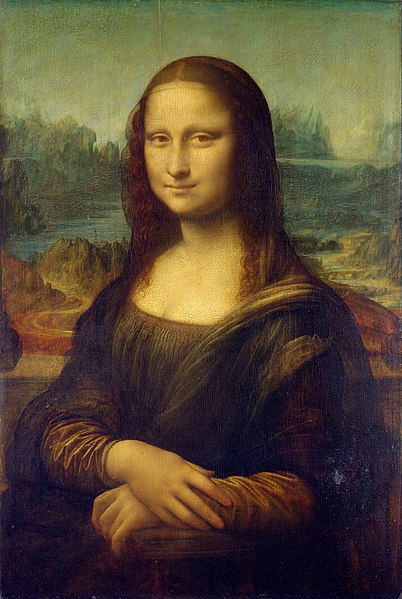
\includegraphics{monalisa}
	\caption[The Mona Lisa]{The Mona Lisa.\\ 
	\url{https://commons.wikimedia.org/wiki/File:Mona_Lisa,_by_Leonardo_da_Vinci,_from_C2RMF_retouched.jpg}}
	\labfig{marginmonalisa}
\end{marginfigure}

The order of the title pages, table of contents and preface can be 
easily changed, as in aly \LaTeX\ document. In addition, the class is 
based on \KOMAScript's \Class{scrbook}, therefore it inherits all the 
goodies of that.

\section{What this class does not}
\labsec{doesnot}

As anticipated, further customisation of the book is left to the user. 
Indeed, every book may have sidenotes, margin figures and so on, but 
each book will have its own fonts, toc style, special environments and 
so on. For this reason, in addition to the class, we provide only 
sensible defaults, but if these features are not nedded, they can be 
left out. These special packages are located in the \Path{style} 
directory, which is organised as follows:

\begin{description}
	\item[style.sty] This package contains the specifications of page 
	layout, headers and footers, chapter headings, and the fonts used 
	throughout the document.
	\item[packages.sty] Loads additional packages to decorate the 
	writing with special contents (for instance, the \Package{listing} 
	package is loaded here as it is not required in every book). There 
	are also defined some useful commands to print the same words always 
	in the same way, \eg latin words in italics or \Package{packages} in 
	verbatim.
	\item[references.sty] Some useful commands to manage labeling and 
	referencing, again to ensure that the same elements are referenced 
	always in a consistent way.
	\item[environments.sty] Provides special environments, like boxes. 
	Both simple and complex environments are available; by complex we 
	mean that they are endowed with a counter, floating and can be put 
	in a special table of contents.\sidenote[-2mm][]{See 
	\vrefch{mathematics} for some examples.}
	\item[theorems.sty] The style of mathematical environments. 
	Acutally, there are two such packages: one is for plain theorems, 
	\ie the theorems are printed in plain text; the other uses 
	\Package{mdframed} to draw a box around theorems. You can plug the 
	most appropriate style into its document.
\end{description}

\marginnote[2mm]{The audacious users might feel tempted to edit some of 
these packages. I'd be immensely happy if they sent me examples of what 
they have been able to do!}

In the rest of the book, I shall assume that the reader is not a novice 
in the use of \LaTeX, and refer to the documentation of the packages 
used in this class for things that are already explained there. 
Moreover, I assume that the reader is willing to make minor edits to the 
provided packages for styles, environments and commands, if he or she 
does not like the default settings.

\include{%
  mainmatter/existing-instruction-selection-techniques-and-representations%
}
% Copyright (c) 2017-2018, Gabriel Hjort Blindell <ghb@kth.se>
%
% This work is licensed under a Creative Commons Attribution-NoDerivatives 4.0
% International License (see LICENSE file or visit
% <http://creativecommons.org/licenses/by-nc-nd/4.0/> for details).

\chapter{Constraint Programming}
\labelChapter{constraint-programming}

\glsreset{CP}
\glsreset{IP}

This chapter describes \gls{CP}, which is a method for solving combinatorial
problems.
%
Like similar methods such as \gls!{IP} and \gls!{SAT}, in \gls{CP} we first
\emph{model} the problem and then we \emph{solve} the model.
%
The modeling and solving aspects are described in \refSectionList{cp-modeling,
  cp-solving}, respectively.
%
Comprehensive overviews of \gls{CP}, \gls{IP}, and \gls{SAT} are given in
\cite{RossiEtAl:2006}, \cite{Wolsey:1998}, and \cite{BiereEtAl:2009},
respectively.
%
In \refSection{cp-lazy-clause-generation} we briefly describe \glsdesc{LCG},
which is a solving technique that \gls{Chuffed} -- the \gls{constraint solver}
used in the experiments -- is based.

In terms of modeling, \gls{CP} offers a higher level of abstraction compared to
other methods.
%
For example, \gls{CP} provides dedicated \glspl{constraint} for capturing many
recurring problem structures that must be decomposed and reformulated in
\gls{IP} or \gls{SAT}.
%
This makes \gls{CP} particularly suited for modeling the problems introduced in
\refChapter{introduction}.


\section{Modeling}
\labelSection{cp-modeling}

To solve a problem using \gls{CP}, it must first be formulated as a
\gls{constraint model}.
%
Modeling strategies are discussed in detail by \textcite{Smith:2006}.

A \gls!{constraint model} (or just \glsshort!{constraint model}) consists of two
components:%
%
\begin{inlinelist}[itemjoin={, }, itemjoin*={, and}]
  \item a set of \glspl{variable}
  \item a set of \glspl{constraint}
\end{inlinelist}.
%
\Glspl!{variable} represent problem decisions and take their values from a
finite \gls{domain}.
%
The \gls!{domain} of a variable~$\mVar{x}$, denoted $\mDomain(\mVar{x})$, is
typically is a set of integers, but it can also consist of real numbers and
complex structures such as string, sets, and \glspl{graph}~\cite{Gervet:2006}.
%
A \gls{variable}~$\mVar{x}$ is \gls!{assigned.v} if
\mbox{$|\!\mDomain(\mVar{x})| = 1$}, and we abbreviate a \gls{variable}
assignment \mbox{$\mVar{x} \in \mSet{v}$} to \mbox{$\mVar{x} = v$}.

\Glspl!{constraint} express relations between \glspl{variable} and forbid
assignments that are illegal in the problem.
%
Given a set of \glspl{variable} \mbox{$\mVar{x}_1, \ldots, \mVar{x}_k$} and a
\gls{constraint}~$C$, an assignment to \mbox{$\mVar{x}_1, \ldots, \mVar{x}_k$}
is a \gls!{solution}[ to $C$] if \mbox{$C(\mVar{x}_1, \ldots, \mVar{x}_k)$}
holds.
%
An assignment to all \glspl{variable} fulfilling all \glspl{constraint} in a
\glsshort{constraint model}~$M$ is a \gls!{solution}[ to $M$].
%
An example of a \gls{constraint model} and its \glspl{solution} is shown in
\refTable{cp-model-example}.

\begin{table}
  \centering%
  \figureFont\figureFontSize%
  \mbox{}%
  \hfill\hfill%
  \subcaptionbox{Constraint model\labelTable{cp-model-example-instance}}%
                {%
                  \begin{tabular}{lc}
                    \toprule
                      \multicolumn{1}{c}{\tabhead variables}
                        & \tabhead constraints\\
                    \midrule
                      $\mVar{x} \in \mSet{1, 2}$ & $\mVar{x} \neq \mVar{y}$\\
                      $\mVar{y} \in \mSet{1, 2}$ & $\mVar{x} \neq \mVar{z}$\\
                      $\mVar{z} \in \mSet{1, 2, 3, 4}$
                        & $\mVar{y} \neq \mVar{z}$\\
                    \bottomrule
                  \end{tabular}%
                }%
  \hfill%
  \subcaptionbox{Solutions\labelTable{cp-model-example-solutions}}%
                [21mm]%
                {%
                  \newcolumntype{C}{>{$}c<{$}}%
                  $\begin{tabular}{C@{\quad}C@{\quad}C}
                     \toprule
                       \mVar{x} & \mVar{y} & \mVar{z} \\
                     \midrule
                       1 & 2 & 3 \\
                       2 & 1 & 3 \\
                       1 & 2 & 4 \\
                       2 & 1 & 4 \\
                     \bottomrule
                   \end{tabular}$%
                }%
  \hfill\hfill%
  \mbox{}

  \caption[Example of a constraint model]%
          {%
            Example of a constraint model, corresponding to a problem where
            three variables must be assigned values which are different from one
            another%
          }
  \labelTable{cp-model-example}
\end{table}

The use of \glspl{variable} and \glspl{constraint} results in \glspl{constraint
  model} that are \gls!{compositional.cm}, meaning they can easily be
extended to capture additional problems to be solved in unison.


\subsection{Global Constraints}

If a \gls!{binary.c}[ \gls{constraint}] is a \gls{constraint} involving two
\glspl{variable}, then a \gls!{global.c}[ \gls{constraint}] is a
\gls{constraint} over an arbitrary number of
\glspl{variable}~\cite{VanHoeveKatriel:2006}.
%
\Gls{global.c} \glspl{constraint} capture recurring problem structures and
improve solving compared to relations modeled using multiple \gls{binary.c}
\glspl{constraint}.


\paragraph{The All-Different Constraint}

Arguably, the most well-known \gls{global.c} \gls{constraint} is the
\gls!{all-different constraint}~\cite{Lauriere:1978} (see~\cite{VanHoeve:2001}
for a survey), which enforces all \glspl{variable} in a given set to take
distinct values.
%
We refer to this \gls{constraint} as $\mAllDifferent$, which is defined as
follows.

\begin{definition}[$\mAllDifferent$]
  Let \mbox{$\mVar{x}_1, \ldots, \mVar{x}_k$} be a list of \glspl{variable}.
  %
  Then
  %
  \begin{displaymath}
    \mAllDifferent(\mVar{x}_1, \ldots, \mVar{x}_k)
    \equiv
    \mBigAnd_{\mathclap{1 \,\leq\, i \,<\, j \,\leq\, k}}
    \mVar{x}_i \neq \mVar{x}_j.
  \end{displaymath}
  \labelDefinition{all-different}
\end{definition}

Hence the \glspl{constraint} in \refTable{cp-model-example} can be replaced by
$\mAllDifferent(\mVar{x}, \mVar{y}, \mVar{z})$.


\paragraph{The Global Cardinality Constraint}

In \refChapter{existing-isel-techniques-and-reps} we saw another \gls{global.c}
\gls{constraint} -- the \gls!{global cardinality
  constraint}~\cite{OplobeduEtAl:1989} -- and how it can be used to model the
\gls{pattern selection} problem (see \refEquation{pattern-selection-using-gcc}
on \refPageOfEquation{pattern-selection-using-gcc}).
%
This \gls{constraint} is a generalization of the \gls{all-different constraint},
and for completeness we give here the its formal definition.

\begin{definition}[$\mGCC$]
  Let \mbox{$v_1, \ldots, v_k$} be a list of values, and let \mbox{$\mVar{x}_1,
    \ldots, \mVar{x}_n$} and \mbox{$\mVar{c}_1, \ldots, \mVar{c}_k$} be lists of
  \glspl{variable}.
  %
  Then
  %
  \begin{displaymath}
    \mGCC(
      \mTuple{v_1, \mVar{c}_1} \hspace{-1pt},
      \ldots,
      \mTuple{v_k, \mVar{c}_k}  \hspace{-1pt},
      \mVar{x}_1, \ldots, \mVar{x}_n
    )
    \equiv
    \mBigAnd_{\mathclap{1 \,\leq\, i \,\leq\, k}}
    \big|
      \mSetBuilder{\mVar{x}_j}{\forall 1 \leq j \leq n : \mVar{x}_j = v_i}
    \big| = \mVar{c}_i.
  \end{displaymath}
  \labelDefinition{gcc}
\end{definition}

For example, \mbox{$\mGCC(\mTuple{5, \mVar{c}_1 = 0} \hspace{-1pt}, \mTuple{3,
    \mVar{c}_2 = 1} \hspace{-1pt}, \mVar{x}_1 = 2, \mVar{x}_2 = 3)$} holds
because no $\mVar{x}$~\gls{variable} is assigned value~\num{5} and exactly one
$\mVar{x}$~\gls{variable} is assigned value~\num{3}.
%
Similarly, \mbox{$\mGCC(\mTuple{3, \mVar{c}_1 \in \mSet{0, 2}} \hspace{-1pt},
  \mVar{x}_1 = 2, \mVar{x}_2 = 3)$} does not holds because either none or both
$\mVar{x}$~\glspl{variable} must be assigned value~\num{3}.


\paragraph{The Circuit Constraint}

Another relevant example is the \gls!{circuit constraint}~\cite{Lauriere:1978},
which enforces that the \glspl{variable} representing adjacency forms a
\gls{Hamiltonian.c} \gls{cycle}.
%
We refer to this \gls{constraint} as $\mCircuit$, which is defined as follows.

\begin{definition}[$\mCircuit$]
  Let \mbox{$\mVar{x}_1, \ldots, \mVar{x}_k$} be a list of \glspl{variable}, and
  let \mbox{$P = d_1, \ldots, d_k$} be a permutation of \gls{domain} values such
  that \mbox{$d_i \in \mDomain(\mVar{x}_i)$} for all \mbox{$i = 1, \ldots,
    k$\hspace{-.8pt}.}
  %
  Given $P$, form a \gls{graph}~\mbox{$G = \mPair{N}{E}$} such that there is
  exactly one \gls{node} \mbox{$n_i \in N$} and exactly one \gls{edge}
  \mbox{$\mEdge{n_i}{n_{d_i}}$} for all \mbox{$i = 1, \ldots, k$\hspace{-.8pt}.}
  %
  $P$ is considered \emph{cyclic} if and only if $G$ contains a
  \gls{Hamiltonian.c} \gls{cycle}.
  %
  Then
  %
  \begin{displaymath}
    \mCircuit(\mVar{x}_1, \ldots, \mVar{x}_k)
    \equiv
    \text{$\mVar{x}_1, \ldots, \mVar{x}_k$ is cyclic}.
  \end{displaymath}
  \labelDefinition{circuit}
\end{definition}

For example, \mbox{$\mCircuit(\mVar{x}_1 \in \mSet{2}, \mVar{x}_2 \in \mSet{4},
  \mVar{x}_3 \in \mSet{1}, \mVar{x}_4 \in \mSet{3})$} holds because the
assignment forms the following \gls{cycle}:
%
\begin{center}
  \figureFont\figureFontSize%
  \begin{tikzpicture}[%
      every node/.style={
        node distance=4mm,
      }
    ]

    \node (x1) {$\mVar{x}_1$};
    \node [right=of x1] (x2) {$\mVar{x}_2$};
    \node [below=of x1] (x3) {$\mVar{x}_3$};
    \node [right=of x3] (x4) {$\mVar{x}_4$};

    \begin{scope}[->, line width=\normalLineWidth]
      \draw (x1) -- (x2);
      \draw (x2) -- (x4);
      \draw (x4) -- (x3);
      \draw (x3) -- (x1);
    \end{scope}
  \end{tikzpicture}%
\end{center}
%
However, \mbox{$\mCircuit(\mVar{x}_1 \in \mSet{2}, \mVar{x}_2 \in \mSet{1},
  \mVar{x}_3 \in \mSet{4}, \mVar{x}_4 \in \mSet{3})$} does not hold because the
assignment forms two non-\gls{Hamiltonian.c} \glspl{cycle}:
%
\begin{center}
  \figureFont\figureFontSize%
  \begin{tikzpicture}[%
      every node/.style={
        node distance=4mm,
      }
    ]

    \node (x1) {$\mVar{x}_1$};
    \node [right=of x1] (x2) {$\mVar{x}_2$};
    \node [below=of x1] (x3) {$\mVar{x}_3$};
    \node [right=of x3] (x4) {$\mVar{x}_4$};

    \begin{scope}[->, line width=\normalLineWidth, bend left]
      \draw (x1) to (x2);
      \draw (x2) to (x1);
      \draw (x3) to (x4);
      \draw (x4) to (x3);
    \end{scope}
  \end{tikzpicture}%
\end{center}

$\MCircuit$ is used in \refChapter{constraint-model} to model \gls{block
  ordering}.


\paragraph{The Table Constraint}

The \gls!{table constraint} constrains a list of \glspl{variable} such that the
values appear as a row in a given matrix.
%
By encoding legal \gls{variable} assignments into the matrix, any relation can
be expressed using a \gls{table constraint}, thus belonging to a group of
so-called \glspl!{extensional
  constraint}~\cite[Sect.\thinspace11.5.4]{Smith:2006}.
%
We refer to this \gls{constraint} as $\mTable$, which is defined as follows.

\begin{definition}[$\mTable$]
  Let \mbox{$\mVar{x}_1, \ldots, \mVar{x}_k$} be a list of \glspl{variable}, and
  let $T$ be an \mbox{$m \times k$} matrix, where \mbox{$m \in \mathbb{N}$}.
  %
  Then
  %
  \begin{displaymath}
    \mTable(
      \mTuple{\mVar{x}_1, \ldots, \mVar{x}_k} \hspace{-1pt},
      T
    )
    \equiv
    \mTuple{\mVar{x}_1, \ldots, \mVar{x}_k} \in T\!.
  \end{displaymath}
  \labelDefinition{table}
\end{definition}

For example, assume we are given a matrix
%
\begin{displaymath}
    A =
    \begin{aMatrix}{cc}
      1 & 1 \\
      2 & 4
    \end{aMatrix}\!\!.
\end{displaymath}
%
Then \mbox{$\mTable(\mVar{x}_1 = 2, \mVar{x}_2 = 4, A)$} holds because the tuple
\mbox{$\mTuple{2, 4}$} appears as a row in~$A$.
%
Similarly, \mbox{$\mTable(\mVar{x}_1 = 3, \mVar{x}_2 = 3, A)$} does not hold
because the tuple \mbox{$\mTuple{3, 3}$} appears as a row in~$A$.

$\MTable$ is used in \refChapter{solving-techniques} to refine the
\glsshort{constraint model} and to model several of the solving techniques.


\paragraph{The Value-Precede-Chain Constraint}
\labelSection{cp-vpc}

The \gls!{value-precede-chain constraint}~\cite{LawLee:2004} requires a list of
\glspl{variable} to be sorted according to a given chain of values.
%
We refer to this \gls{constraint} as $\mValuePrecChain$, which is defined as
follows.

\begin{definition}[$\mValuePrecChain$]
  Let \mbox{$c_1, \ldots, c_n$} be a list of values and \mbox{$\mVar{x}_1,
    \ldots, \mVar{x}_k$} be a list of \glspl{variable}.
  %
  Then
  %
  \begin{displaymath}
    \mValuePrecChain(c_1, \ldots, c_n, \mVar{x}_1, \ldots, \mVar{x}_k)
    \equiv
    \mBigAnd_{
      \mathclap{
        \substack{
          1 \,\leq\, i \,\leq\, k \hspace{-.8pt}, \\
          1 \,\leq\, j \,<\, n \phantom{\hspace{-.8pt},}
        }
      }
    }
    \mVar{x}_i = c_{j+1} \mImp (\exists l < j : \mVar{x}_l = c_j).
  \end{displaymath}
  \labelDefinition{vpc}
\end{definition}

For example, \mbox{$\mValuePrecChain(6, 5, 4, \mVar{x}_1 = 6, \mVar{x}_2 = 1,
  \mVar{x}_3 = 5, \mVar{x}_4 = 4)$} holds because the~\num{4} is preceded by
a~\num{5}, which in turn is preceded by a~\num{6}, in the list of
$\mVar{x}$~\glspl{variable}.
%
Likewise, \mbox{$\mValuePrecChain(5, 4, \mVar{x}_1 = 5, \mVar{x}_2 = 1)$} also
holds because \num{4} does not appear among the $\mVar{x}$~\glspl{variable} (the
fact that \num{5} appears in the list does not matter).
%
However, \mbox{$\mValuePrecChain(5, 4, \mVar{x}_1 = 1, \mVar{x}_2 = 4)$} does
not hold because the~\num{4} is not preceded by a~\num{5}.

$\MValuePrecChain$ is used in \refChapter{solving-techniques} to implement a
\gls{dominance breaking.c} \gls{constraint}.


\paragraph{The Cumulative Constraint}
\labelSection{cp-cumulative}

The \gls!{cumulative constraint}~\cite{AggounBeldiceanu:1993} is used in
scheduling to constrains the scheduling times for a given set of tasks such that
the capacity of a given resource is not exceeded.
%
We refer to this \gls{constraint} as $\mCumulative$, which is defined as
follows.
%
\begin{definition}[$\mCumulative$]
  Let \mbox{$c \in \mNatNumSet$} represent the capacity of a resource to be used
  by $k$ optional tasks.
  %
  For each task~\mbox{$i = 1, \ldots, k$}, let \mbox{$\mVar{s}_i \in
    \mNatNumSet$} be a \gls{variable} representing the time at which $i$ is
  scheduled to start, and \mbox{$\mVar{b}_i \in \mSet{0, 1}$} be a
  \gls{variable} representing whether $i$ is scheduled.
  %
  Let also \mbox{$l_i \in \mNatNumSet$} represent task~$i$'s duration, and
  \mbox{$u_i \in \mNatNumSet$} represent the amount of resource required by~$i$,
  %
  Lastly, let \mbox{$t_{\mathsc{max}} = \mMax(\cup_{1 \,\leq\, j \,\leq\, k}
    \mDomain(\mVar{s}_j))$}.
  %
  Then
  %
  \begin{displaymath}
    \mCumulative(
      c \hspace{-1pt},
      \mTuple{
        \mVar{s}_1 \hspace{-.8pt},
        l_1 \hspace{-.8pt},
        u_1 \hspace{-.8pt},
        \mVar{b}_1
      } \hspace{-1pt},
      \ldots,
      \mTuple{
        \mVar{s}_k \hspace{-.8pt},
        l_k \hspace{-.8pt},
        u_k \hspace{-.8pt},
        \mVar{b}_k
      }
    )
    \equiv
    \mBigAnd_{\mathclap{0 \,\leq\, t \,<\, t_{\mathsc{max}}}}
    \hspace{26pt}
    \sum_{
           \mathclap{
             \substack{
               1 \,\leq\, i \,\leq\, k \hspace{-.8pt} \text{ \st} \\
               \mVar{s}_i \,\leq\, t \,<\, \mVar{s}_i \,+\, l_i
             }
           }
         }
    \mVar{b}_i \times u_i
    \leq c \hspace{-1pt}.
  \end{displaymath}
  \labelDefinition{cumulative}
\end{definition}

For example, the schedule shown in \refFigure{cumulative-example-solution} is a
\gls{solution} to this \gls{constraint} because at no time is the capacity
exceeded.
%
\begin{figure}
  \subcaptionbox{A solution\labelFigure{cumulative-example-solution}}%
                {%
                  \input{%
                    figures/constraint-programming/cumulative-example-solution%
                  }%
                }%
  \hfill%
  \subcaptionbox{%
                  Not a solution; the capacity is exceeded%
                  \labelFigure{cumulative-example-failure}%
                }%
                [60mm]%
                {%
                  \input{%
                    figures/constraint-programming/cumulative-example-failure%
                  }%
                }

  \caption[Examples illustrating the cumulative constraint]%
          {%
            Examples illustrating the cumulative constraint.
            %
            Each box represents a task%
          }
  \labelFigure{cumulative-example}
\end{figure}
%
Likewise, the schedule shown in \refFigure{cumulative-example-failure} is not a
\gls{solution} because tasks~$t_4$ and~$t_5$ exceed the capacity when scheduled
in parallel.

$\MCumulative$ is used in \refChapter{proposed-model-extensions} to model
\gls{instruction scheduling}.


\paragraph{The No-Overlap Constraint}
\labelSection{cp-no-overlap}

The last \gls{global.c} \gls{constraint} we will look at is the \gls!{no-overlap
  constraint} (often also called the \gls!{diffn
  constraint}~\cite{BeldiceanuContejean:1994}), which is used in rectangle
packing problems to enforce that no two rectangles may overlap.
%
We refer to this \gls{constraint} as $\mNoOverlap$, which is defined as follows.
%
\begin{definition}[$\mNoOverlap$]
  For each rectangle~$i$, let \mbox{$\mVar{xl}_i, \mVar{xr}_i, \mVar{yl}_i,
    \mVar{yu}_i \in \mNatNumSet$} be \glspl{variable} representing the
  rectangle's left, right, lower, respectively upper boundary.
  %
  Then
  %
  \begin{displaymath}
    \begin{array}{c}
      \mNoOverlap(
        \mTuple{
          \mVar{xl}_1 \hspace{-.8pt},
          \mVar{xr}_1 \hspace{-.8pt},
          \mVar{yl}_1 \hspace{-.8pt},
          \mVar{yu}_1 \hspace{-.8pt}
        } \hspace{-1pt},
        \ldots,
        \mTuple{
          \mVar{xl}_k \hspace{-.8pt},
          \mVar{xr}_k \hspace{-.8pt},
          \mVar{yl}_k \hspace{-.8pt},
          \mVar{yu}_k \hspace{-.8pt}
        }
      )
      \equiv \mbox{} \\
      \displaystyle\mBigAnd_{\mathclap{1 \,\leq\, i \,<\, j \,\leq\, k}}
      \mVar{xr}_i \leq \mVar{xl}_j \mOr
      \mVar{xr}_j \leq \mVar{xl}_i \mOr
      \mVar{yu}_i \leq \mVar{yl}_j \mOr
      \mVar{yu}_j \leq \mVar{yl}_i \hspace{-1pt}.
    \end{array}
  \end{displaymath}
  \labelDefinition{no-overlap}
\end{definition}

For example, \refFigure{no-overlap-example-solution} is a \gls{solution} to this
\gls{constraint} because the two squares do not overlap.
%
Likewise, \refFigure{no-overlap-example-failure} is a not \gls{solution} because
the squares do overlap.

\begin{figure}
  \mbox{}%
  \hfill\hfill%
  \subcaptionbox{A solution\labelFigure{no-overlap-example-solution}}%
                {%
                  \input{%
                    figures/constraint-programming/no-overlap-example-solution%
                  }%
                }%
  \hfill%
  \subcaptionbox{Not a solution\labelFigure{no-overlap-example-failure}}%
                [30mm]%
                {%
                  \input{%
                    figures/constraint-programming/no-overlap-example-failure%
                  }%
                }%
  \hfill\hfill%
  \mbox{}

  \caption{Examples illustrating the no-overlap constraint}%
  \labelFigure{no-overlap-example}
\end{figure}

$\MNoOverlap$ is used in \refChapter{proposed-model-extensions} to model
\gls{register allocation}.


\subsection{Optimization}

An optimization problem is modeled by maximizing or minimizing a
\gls{variable}~$\mVar{c}$ whose value is constrained according to an
\gls{objective function}.
%
For example, if \mbox{$\mVar{x}_m \in \mSet{0, 1}$} is \gls{variable}
representing whether a \gls{match}~$m$ is selected and $c_m$ denotes the cost of
selecting~\mbox{$m$\hspace{-.8pt},} then a \gls{CP} idiom for modeling
\gls{optimal.ps} \gls{pattern selection} is
%
\begin{equation}
  \begin{array}{rl}
      \text{minimize} & \mVar{c} \\
    \text{subject to} & \mVar{c} = \displaystyle\sum_m c_m \mVar{x}_m
  \end{array}
  \labelEquation{pattern-selection-in-cp}
\end{equation}
%
In this context, $\mVar{c}$ is called a \gls!{cost variable}.
%
Note that the \gls{objective function} is orthogonal to the rest of the
\glsshort{constraint model}, thus allowing it to be easily customized to fit the
desired optimization criterion.


\section{Solving}
\labelSection{cp-solving}

A \gls!{constraint solver} (or just \gls!{solver}) finds \glspl{solution} to a
\gls{constraint model} by interleaving \gls{propagation} and \gls{search}.
%
\Gls!{propagation} removes \gls{domain} values that are known to be in conflict
with a \gls{constraint}, and \gls!{search} attempts several alternatives when
\gls{propagation} alone is insufficient for finding a \gls{solution}.

In practice, however, this alone is often not enough for many problem instances
as the \gls{search space} is simply too large.
%
In such cases, the \gls{search space} can be further reduced by extending the
\gls{constraint model} with additional \glspl{constraint} to strengthen
propagation and remove uninteresting \glspl{solution} and by performing
\gls{presolving}.


\subsection{Propagation}
\labelSection{cp-propagation}

Performing \gls{propagation} requires an array of \gls{domain}-pruning
algorithms and a system that allows these algorithms to interact.
%
\Gls{propagation} theory is discussed in detail by \textcite{Bessiere:2006}, and
\glsdesc{CP} systems are thoroughly discussed by
\textcite{SchulteCarlsson:2006}.

\Gls{constraint solver} typically keep track of \glspl{variable} and their
\glspl{domain} using \glspl{constraint store}.
%
A \gls!{constraint store} (or just \gls!{store}) is a data structure that maps a
set of \glspl{variable} to sets of \glspl{domain}.
%
A \gls{store}~$S_1$ is \gls!{stronger.cs} than another \gls{store}~$S_2$,
denoted \mbox{$S_1 \mStronger S_2$}, if \mbox{$\mDomain_1(\mVar{x}) \subseteq
  \mDomain_2(\mVar{x})$} for all \glspl{variable}~$\mVar{x}$, where
$\mDomain_i(\mVar{x})$ denotes the domain of \gls{variable}~$\mVar{x}$ in
store~$S_i$.

A function that takes a \gls{constraint store} as input and produces another
\gls{store} is called a \gls!{propagator} (or \gls!{filtering algorithm}).
%
A \gls{propagator} implements a \gls{constraint} if it does not remove any
\glspl{solution} to the \gls{constraint} and only keeps \gls{variable}
assignments that are part of a \gls{solution}.
%
For solving to be well-behaved, \glspl{propagator} are also expected to be
\gls!{decreasing.p} -- it does not add any values, hence \mbox{$p(S) \mStronger
  S$} -- and \gls!{monotonic.p} -- if \mbox{$S_1 \mStronger S_2$}, then
\mbox{$p(S_1) \mStronger p(S_2)$}.
%
A \gls{propagator} for which \mbox{$p(S) = S$} holds is said to be at
\gls!{fixpoint}, and a \gls{store} is at \gls{fixpoint} if all
\glspl{propagator} are at \gls{fixpoint} for that \gls{store}.
%
A \gls{propagator} that returns a \gls{store} with at least one empty
\gls{domain} has \glsshort!{failure}, meaning there are no \glspl{solution} in
that part of the \gls{search space}.

\Glspl{propagator} implementing the same \gls{constraint} can differ in the
amount of propagation they perform.
%
A \gls{propagator} is \glshyphened!{value consistency} if it only
\glsshort{propagation}[es] when one of its \glspl{variable} becomes
\gls{assigned.v}, \glshyphened!{bounds consistency} if it only reduces the
bounds of a \gls{domain}, and \glshyphened!{domain consistency} if it removes
all values that do not appear in any \gls{solution} to the \gls{constraint}.
%
For example, \refTable{cp-prop-strengths-example} shows solving of two versions
of the \glsshort{constraint model} given in \refTable{cp-model-example}, one
using $\mAllDifferent$ and another using inequality \glspl{constraint}.
%
\begin{table}
  \centering%
  \figureFont\figureFontSize%
  \newcolumntype{C}{>{$}c<{$}}%
  \subcaptionbox{%
                  Solving with value-consistent inequality constraints%
                  \labelTable{cp-prop-strengths-example-inequality-cons}%
                }{%
                  \begin{tabular}{%
                                   p{4.5cm}%
                                   C@{}C@{ }C@{}C%
                                   C@{}C@{ }C@{}C%
                                   C@{}C@{ }C@{ }C@{ }C@{}C%
                                 }
                    \toprule
                      \multicolumn{1}{c}{\tabhead event}
                        & \multicolumn{14}{c}{\tabhead store}\\
                      \cmidrule(lr){2-15}%
                        & \multicolumn{4}{c}{$\mVar{x}$}
                        & \multicolumn{4}{c}{$\mVar{y}$}
                        & \multicolumn{6}{c}{$\mVar{z}$}\\
                    \midrule
                      Initial store
                        & \{ & 1, & 2  & \}
                        & \{ & 1, & 2  & \}
                        & \{ & 1, & 2, & 3, & 4 & \}\\
                      Propagate until fixpoint
                        & \{ & 1, & 2  & \}
                        & \{ & 1, & 2  & \}
                        & \{ & 1, & 2, & 3, & 4 & \}\\
                      Search by attempting $\mVar{z} = 1$
                        & \{ & 1, & 2  & \}
                        & \{ & 1, & 2  & \}
                        & \{ & 1\phantom{,}
                                  &    &    &   & \}\\
                      Propagate $\mVar{y} \neq \mVar{z}$
                        & \{ & 1, & 2  & \}
                        & \{ &    & 2  & \}
                        & \{ & 1\phantom{,}
                                  &    &    &   & \}\\
                      Propagate $\mVar{x} \neq \mVar{z}$
                        & \{ &    & 2  & \}
                        & \{ &    & 2  & \}
                        & \{ & 1\phantom{,}
                                  &    &    &   & \}\\
                      Propagate $\mVar{x} \neq \mVar{y}$
                        & \{ &    &    & \}
                        & \{ &    & 2  & \}
                        & \{ & 1\phantom{,}
                                  &    &    &   & \}\\
                      Failure reached; backtrack
                        & \{ & 1, & 2  & \}
                        & \{ & 1, & 2  & \}
                        & \{ &    & 2, & 3, & 4 & \}\\
                      \qquad\raisebox{0pt}[10pt]{$\vdots$}
                        & & & & & & & & & & & & & & \\[-2pt]
                    \bottomrule
                  \end{tabular}%
                }

  \vspace{\betweensubfigures}

  \subcaptionbox{%
                  Solving with domain-consistent all-different constraint%
                  \labelTable{cp-prop-strengths-example-alldiff}%
                }{%
                  \begin{tabular}{%
                                   p{4.5cm}%
                                   C@{}C@{ }C@{}C%
                                   C@{}C@{ }C@{}C%
                                   C@{}C@{ }C@{ }C@{ }C@{}C%
                                 }
                    \toprule
                      \multicolumn{1}{c}{\tabhead event}
                        & \multicolumn{14}{c}{\tabhead store}\\
                      \cmidrule(lr){2-15}%
                        & \multicolumn{4}{c}{$\mVar{x}$}
                        & \multicolumn{4}{c}{$\mVar{y}$}
                        & \multicolumn{6}{c}{$\mVar{z}$}\\
                    \midrule
                      Initial store
                        & \{ & 1, & 2  & \}
                        & \{ & 1, & 2  & \}
                        & \{ & 1, & 2, & 3, & 4 & \}\\
                      Propagate $\mAllDifferent(\mVar{x}, \mVar{y}, \mVar{z})$
                        & \{ & 1, & 2  & \}
                        & \{ & 1, & 2  & \}
                        & \{ &    &    & 3, & 4 & \}\\
                      \qquad\raisebox{0pt}[10pt]{$\vdots$}
                        & & & & & & & & & & & & & & \\[-2pt]
                    \bottomrule
                  \end{tabular}%
                }

  \caption[Example illustrating propagation]%
          {%
            Example illustrating propagation for two versions of the model given
            in \refTable{cp-model-example}, one using the all-different
            constraint and the other using a binary decomposition%
          }
  \labelTable{cp-prop-strengths-example}
\end{table}
%
Because only \gls{value consistency} can be achieved for inequality
\glspl{constraint}, they cannot \glsshort{propagation}[e] anything until at
least one \gls{variable} becomes \gls{assigned.v}
(\refTable{cp-prop-strengths-example-inequality-cons}).
%
As all \glspl{propagator} are already at \gls{fixpoint}, the \gls{solver} must
resort to \gls{search}.
%
In this case, the \gls{solver} makes a wrong guess and is forced to backtrack.
%
In comparison, a \glshyphened{domain consistency} \gls{propagator} for the
\gls{all-different constraint} can remove values~\num{1} and~\num{2} from the
\gls{domain} of \gls{variable}~$\mVar{z}$ as these values do not appear in any
\glspl{solution} (\refTable{cp-prop-strengths-example-alldiff}).
%
As the \gls{search space} grows exponentially with the number of
\glspl{variable} and size of the \glspl{domain}, maximizing \gls{propagation} is
key in making solving tractable.

As to be expected, stronger \gls{propagation} comes at a price of greater
complexity.
%
For the \gls{all-different constraint}, there exist \glsshort{bounds
  consistency} and \glshyphened{domain consistency} \glspl{propagator} with
worst-case time complexities~$\mBigO(n \log n)$~\cite{Lopez-OrtizEtAl:2003}
and~$\mBigO(n^{2.5})$~\cite{Regin:1994}, respectively, where $n$ denotes the
number of \glspl{variable}.
%
The same can be achieved for the \gls{global cardinality constraint} at similar
cost~\cite{QuimperEtAl:2005, Regin:1996}.

\Gls{domain consistency} for \gls{circuit constraint} cannot be achieved in
polynomial time as it involves finding Hamiltonian cycles, which is
NP-complete~\cite{GareyJohnson:1979}.
%
An incomplete, polynomial-time \gls{filtering algorithm} is given
in~\cite{KayaHooker:2006}.

Several \glshyphened{domain consistency} \gls{propagator} exist for the
\glsshort{table constraint} \cite{LecoutreSzymanek:2006, Lecoutre:2011,
  MairyEtAl:2014, PerezRegin:2014, LecoutreEtAl:2015, DemeulenaereEtAl:2016},
\glsshort{cumulative constraint}~\cite{BaptisteEtAl:2001}, and \gls{no-overlap
  constraint}~\cite{BeldiceanuCarlsson:2001, VanHentenryckEtAl:1998}, but these
exhibit exponential worst-case time complexity.
%
For the \gls{value-precede-chain constraint}, there exist \glshyphened{domain
  consistency} \glspl{propagator} with linear time
complexity~\cite{LawLee:2004}.


\subsection{Search}
\labelSection{cp-search}

When no more \gls{propagation} can be performed -- that is, when all
\glspl{propagator} are at \gls{fixpoint} -- the \gls{solver} resorts to
\gls{search}.
%
This is discussed in detail by \textcite{VanBeek:2006}.

In exploring the \gls{search space}, two decisions need to be made repeatedly:
%
\begin{enumerate*}[label=(\roman*), itemjoin*={, and\ }]
  \item select a \gls{variable} on which to branch
  \item select one or more values (but not all) from its \gls{domain}
\end{enumerate*}.
%
These decisions constitute a \gls!{branching strategy}.
%
The \gls{branching strategy} arranges the \gls{search space} into a \gls!{search
  tree}, where each \gls{node} represents a \gls{store} at \gls{fixpoint} (see
\refFigure{cp-search-tree-sat-example} for an example).
%
\begin{figure}
  \centering%
  % Copyright (c) 2017-2018, Gabriel Hjort Blindell <ghb@kth.se>
%
% This work is licensed under a Creative Commons Attribution-NoDerivatives 4.0
% International License (see LICENSE file or visit
% <http://creativecommons.org/licenses/by-nc-nd/4.0/> for details).
%
\begingroup%
\figureFont\figureFontSize%
\newcolumntype{C}{@{}c@{}}%
\def\lineWidth{.8pt}
\def\nodeDist{36pt}
\begin{tikzpicture}[%
    intermediate node/.style={%
      nothing,
      draw,
      circle,
      line width=\lineWidth,
      fill=white!50!shade1,
      font=\smaller,
      node distance=\nodeDist,
    },
    solution/.style={%
      intermediate node,
      diamond,
    },
    branch/.style={%
      line width=\lineWidth,
    },
    branch label/.style={%
      nothing,
      inner sep=2pt,
      auto,
      pos=.4,
    },
  ]

  \node [solution] (sol1)
        {%
          $%
            \begin{array}{C}
              \mVar{x} \in \mSet{1} \\
              \mVar{y} \in \mSet{2} \\
              \mVar{z} \in \mSet{3} \\
            \end{array}
          $%
        };
  \node [solution, right=of sol1] (sol2)
        {%
          $%
            \begin{array}{C}
              \mVar{x} \in \mSet{1} \\
              \mVar{y} \in \mSet{2} \\
              \mVar{z} \in \mSet{4} \\
            \end{array}
          $%
        };
  \node [solution, right=of sol2] (sol3)
        {%
          $%
            \begin{array}{C}
              \mVar{x} \in \mSet{2} \\
              \mVar{y} \in \mSet{1} \\
              \mVar{z} \in \mSet{3} \\
            \end{array}
          $%
        };
  \node [solution, right=of sol3] (sol4)
        {%
          $%
            \begin{array}{C}
              \mVar{x} \in \mSet{2} \\
              \mVar{y} \in \mSet{1} \\
              \mVar{z} \in \mSet{4} \\
            \end{array}
          $%
        };
  \node [intermediate node,
         above=.25*\nodeDist of $(sol1.north) !.5! (sol2.north)$] (int1)
        {%
          $%
            \begin{array}{C}
              \mVar{x} \in \mSet{1} \\
              \mVar{y} \in \mSet{2} \\
              \mVar{z} \in \mSet{3, 4} \\
            \end{array}
          $%
        };
  \node [intermediate node,
         above=.25*\nodeDist of $(sol3.north) !.5! (sol4.north)$] (int2)
        {%
          $%
            \begin{array}{C}
              \mVar{x} \in \mSet{2} \\
              \mVar{y} \in \mSet{1} \\
              \mVar{z} \in \mSet{3, 4} \\
            \end{array}
          $%
        };
  \node [intermediate node, above=0 of $(int1.north) !.5! (int2.north)$] (root)
        {%
          $%
            \begin{array}{C}
              \mVar{x} \in \mSet{1, 2} \\
              \mVar{y} \in \mSet{1, 2} \\
              \mVar{z} \in \mSet{3, 4} \\
            \end{array}
          $%
        };

  \begin{scope}[branch]
    \draw (root)
          -- node [branch label, swap] {$\mVar{x} = 1$}
          (int1);
    \draw (root)
          -- node [branch label] {$\mVar{x} \neq 1$}
          (int2);
    \draw (int1)
          -- node [branch label, swap] {$\mVar{z} = 3$}
          (sol1);
    \draw (int1)
          -- node [branch label] {$\mVar{z} \neq 3$}
          (sol2);
    \draw (int2)
          -- node [branch label, swap] {$\mVar{z} = 3$}
          (sol3);
    \draw (int2)
          -- node [branch label] {$\mVar{z} \neq 3$}
          (sol4);
  \end{scope}
\end{tikzpicture}%
\endgroup%


  \caption[Example of a search tree]%
          {%
            Example of a search tree for the model given in
            \refTable{cp-model-example}.
            %
            Diamond-shaped nodes represent solutions%
          }
  \labelFigure{cp-search-tree-sat-example}
\end{figure}
%
Since the \glspl{solution} (and \glspl{failure}) appear at the leaf
\glspl{node}, the \gls{search tree} is typically explored depth-first.


For \gls{search} to be well-behaved, a \gls{branching strategy} must preserve
all \glspl{solution} in the \gls{search space} and must not duplicate any
\gls{solution}.
%
A common strategy in choosing a \gls{variable}, called the \gls!{first-fail
  principle}, is to select the \gls{variable} most likely to cause a
\gls{failure}~\cite{HaralickElliott:1980}.
%
Other strategies involve selecting the \gls{variable} with the smallest or
largest value in its \gls{domain}, or selecting a random \gls{variable}.
%
Similar strategies are applied in value selection, which is typically done by
posting \gls{constraint} when branching.
%
Most common is to post unary \gls{constraint} that divides a \gls{domain} into
an \gls{assigned.v} part an a non-\gls{assigned.v} part.
%
For example, at the root \gls{node} in \refFigure{cp-search-tree-sat-example},
\gls{search} branches on \gls{variable}~$\mVar{x}$ by posting \mbox{$\mVar{x} =
  1$} in one branch and \mbox{$\mVar{x} \neq 1$} in the other.
%
Another strategy is to split the domain by posting inequality \glspl{constraint}
(for example, \mbox{$\mVar{x} \leq 3$} in one branch and \mbox{$\mVar{x} > 3$}
in the other), which is useful for solving \glsplshort{constraint model} with
arithmetic \glspl{constraint}.
%
More than one \gls{branching strategy} can be used for the same
\glsshort{constraint model} and, if needed, they can be customized by the user,
making it a key strength of \gls{CP}.


\paragraph{Branch and Bound}
\labelPage{cp-branch-and-bound}

\Glspl{solution} to optimization problems are found using a method called
\gls!{branch and bound}~\cite{LandDoig:1960}.
%
During \gls{search}, the best \gls{solution} found so far is kept and a
\gls{constraint} is added to enforce all subsequent \glspl{solution} to have
strictly less (or greater) cost.
%
Hence time can be traded for quality on a continuous time scale.
%
When the entire \gls{search space} has been explored, the last found
\gls{solution} is guaranteed to be optimal.
%
An example of shown in \refFigure{cp-search-tree-opt-example}.
%
\begin{figure}
  \centering%
  % Copyright (c) 2017-2018, Gabriel Hjort Blindell <ghb@kth.se>
%
% This work is licensed under a Creative Commons Attribution-NoDerivatives 4.0
% International License (see LICENSE file or visit
% <http://creativecommons.org/licenses/by-nc-nd/4.0/> for details).
%
\begingroup%
\figureFont\figureFontSize%
\newcolumntype{C}{@{}c@{}}%
\def\lineWidth{.8pt}
\def\nodeDist{36pt}
\begin{tikzpicture}[%
    intermediate node/.style={%
      nothing,
      draw,
      circle,
      line width=\lineWidth,
      fill=white!50!shade1,
      font=\smaller,
      node distance=\nodeDist,
    },
    solution/.style={%
      intermediate node,
      diamond,
    },
    failure/.style={%
      solution,
      rectangle,
    },
    branch/.style={%
      line width=\lineWidth,
    },
    branch label/.style={%
      nothing,
      inner sep=2pt,
      auto,
      pos=.4,
    },
    bound label/.style={%
      nothing,
      inner sep=2pt,
      node distance=4pt,
    },
  ]

  \node [solution] (sol1)
        {%
          $%
            \begin{array}{C}
              \mVar{x} \in \mSet{1} \\
              \mVar{y} \in \mSet{2} \\
              \mVar{z} \in \mSet{3} \\
            \end{array}
          $%
        };
  \node [solution, right=of sol1] (sol2)
        {%
          $%
            \begin{array}{C}
              \mVar{x} \in \mSet{1} \\
              \mVar{y} \in \mSet{2} \\
              \mVar{z} \in \mSet{4} \\
            \end{array}
          $%
        };
  \node [solution, right=of sol2, opacity=0] (sol3)% Needed for positioning
        {%
          $%
            \begin{array}{C}
              \mVar{x} \in \mSet{2} \\
              \mVar{y} \in \mSet{1} \\
              \mVar{z} \in \mSet{3} \\
            \end{array}
          $%
        };
  \node [solution, right=of sol3, opacity=0] (sol4)% Needed for positioning
        {%
          $%
            \begin{array}{C}
              \mVar{x} \in \mSet{2} \\
              \mVar{y} \in \mSet{1} \\
              \mVar{z} \in \mSet{4} \\
            \end{array}
          $%
        };
  \node [intermediate node,
         above=.25*\nodeDist of $(sol1.north) !.5! (sol2.north)$] (int1)
        {%
          $%
            \begin{array}{C}
              \mVar{x} \in \mSet{1} \\
              \mVar{y} \in \mSet{2} \\
              \mVar{z} \in \mSet{3, 4} \\
            \end{array}
          $%
        };
  \coordinate (above-sol3-sol4) at ($(sol3.north) !.5! (sol4.north)$);
  \node [failure, minimum size=12mm] at (above-sol3-sol4 |- int1) (fail)
        {%
          $%
            \begin{array}{C}
              \mVar{x} \in \mSet{2} \\
              \mVar{y} \in \mSet{1} \\
              \mVar{z} \in \mSet{} \\
            \end{array}
          $%
        };
  \node [intermediate node, above=0 of $(int1.north) !.5! (fail.north)$] (root)
        {%
          $%
            \begin{array}{C}
              \mVar{x} \in \mSet{1, 2} \\
              \mVar{y} \in \mSet{1, 2} \\
              \mVar{z} \in \mSet{3, 4} \\
            \end{array}
          $%
        };

  \begin{scope}[branch]
    \draw (root)
          -- node [branch label, swap] {$\mVar{x} = 1$}
          (int1);
    \draw (root)
          -- node [branch label] {$\mVar{x} \neq 1$}
          (fail);
    \draw (int1)
          -- node [branch label, swap] {$\mVar{z} = 3$}
          (sol1);
    \draw (int1)
          -- node [branch label] {$\mVar{z} \neq 3$}
          (sol2);
  \end{scope}

  \node [bound label, below=of sol1] {posting \ $\mVar{z} > 3$};
  \node [bound label, below=of sol2] {posting \ $\mVar{z} > 4$};
\end{tikzpicture}%
\endgroup%


  \caption[Example of a search tree for an optimization problem]%
          {%
            Example of a search tree for the model given in
            \refTable{cp-model-example} with the additional requirement that
            the value of $\mVar{z}$ should be maximized.
            %
            The search tree is explored depth first, left to right.
            %
            Diamond-shaped nodes represent solutions and square-shaped nodes
            represent failures%
          }
  \labelFigure{cp-search-tree-opt-example}
\end{figure}
%
Assuming the \gls{search tree} is explored depth first, left to right, the first
solution to be found is \mbox{$S_1 = \mTuple{\mVar{x} = 1, \mVar{y} = 2,
    \mVar{z} = 3}$}.
%
Since the value of $\mVar{z}$ is to be maximized, this causes the
\gls{constraint} \mbox{$\mVar{z} > 3$} to be posted.
%
The next solution to be found is \mbox{$S_2 = \mTuple{\mVar{x} = 1, \mVar{y} =
    2, \mVar{z} = 4}$}, which is clearly better than $S_1$, causing the
\gls{constraint} \mbox{$\mVar{z} > 4$} to be posted.
%
Since the \gls{domain} of $\mVar{z}$ has no value greater than~\num{4}, the
\gls{constraint} \mbox{$\mVar{z} > 4$} causes a \gls{failure} when the exploring
the other branch at the root.
%
At this point the entire \gls{search space} has been explored, making $S_2$ the
optimal \gls{solution}.


\subsection{Solving Techniques}
\labelSection{cp-solving-techniques}

Solving can be improved by applying various solving techniques, which can be
divided into two categories.
%
The first category involves additional \glspl{constraint} that are added to the
\glsshort{constraint model} in order to increase \gls{propagation} and also
reduce the \gls{search space}.
%
These \glspl{constraint} can be divided into three categories --
\gls{implied.c}, \gls{symmetry breaking.c}, and \gls{dominance breaking.c} --
which are discussed in detail by \mbox{\textcite{Smith:2006}},
\textcite{GentEtAl:2006}, and \textcite{ChuStuckey:2015}, respectively.

The second category -- \gls{presolving} -- involves applying methods that reduce
the number of \glspl{variable} or shrink the \gls{variable} \glspl{domain},
thereby reducing the \gls{search space}.


\paragraph{Implied Constraints}

An \gls!{implied.c}[ \gls{constraint}] is a \gls{constraint} that strengthens
\gls{propagation} without removing any \glspl{solution}.
%
For example, assume a naive \glsshort{constraint model} for solving the
\gls!{magic sequence problem}, which is defined as finding a sequence
\mbox{$x_0, \ldots, x_{n-1}$} of integers such that for all \mbox{$0 \leq i <
  n$\hspace{-.8pt},} the number~$i$ appears exactly $x_i$ times in the sequence.
%
Using the \gls{global cardinality constraint} and $n$~\glspl{variable}, this can
be modeled as
%
\begin{equation}
  \mGCC(
    \cup_{0 \,\leq\, i \,<\, n} \mTuple{i, \mVar{x}_i} \hspace{-1pt},
    \mVar{x}_0, \ldots, \mVar{x}_{n-1}
  ).
\end{equation}
%
While this \gls{constraint} is sufficient in capturing the problem,
\gls{propagation} can be increased by adding the following \gls{implied.c}
\gls{constraint}:
%
\begin{equation}
  \sum_{\mathclap{0 \,\leq\, i \,<\, n}} \mVar{x}_i = n.
\end{equation}
%
This always holds because the sum of all occurrences -- that is, the number of
items in the sequence -- must always be equal to the length of the sequence.


\paragraph{Symmetry Breaking Constraints}

A \gls!{symmetry breaking.c}[ \gls{constraint}] is a \gls{constraint} that
removes \glspl{solution} considered to be symmetric to one another.
%
For example, assume a \glsshort{constraint model} for solving a problem of
packing $n$ squares of sizes \mbox{$1, \ldots, n$} inside another, larger
square.
%
Given a \gls{solution} to this problem, more \glspl{solution} can found by
rotating, flipping, and mirroring the initial \gls{solution}.
%
As these \glspl{solution} are essentially the same, only one of them should be
kept in the \gls{search space}.
%
A simple method of removing most (but not all) symmetric \glspl{solution} is to
force one of the squares to be packed into one of the quadrants of the enclosing
square.


\paragraph{Dominance Breaking Constraints}

A \gls!{dominance breaking.c}[ \gls{constraint}] is a \gls{constraint} that
removes \glspl{solution} known to be dominated by another \gls{solution}.
%
\Gls{dominance breaking.c} is therefore a generalization of \gls{symmetry
  breaking.c}.
%
For an example, let us revisit the \glsshort{constraint model} capturing the
square packing problem and assume the two partial \glspl{solution} shown in
\refFigure{square-packing-partial-sol}.
%
\begin{figure}
  \centering%
  \mbox{}%
  \hfill%
  \hfill%
  % Copyright (c) 2017-2018, Gabriel Hjort Blindell <ghb@kth.se>
%
% This work is licensed under a Creative Commons Attribution-NoDerivatives 4.0
% International License (see LICENSE file or visit
% <http://creativecommons.org/licenses/by-nc-nd/4.0/> for details).
%
\begingroup%
\figureFont\figureFontSize%
% Copyright (c) 2017-2018, Gabriel Hjort Blindell <ghb@kth.se>
%
% This work is licensed under a Creative Commons Attribution-NoDerivatives 4.0
% International License (see LICENSE file or visit
% <http://creativecommons.org/licenses/by-nc-nd/4.0/> for details).
%
\figureFont\figureFontSize%
\def\squareSize{10pt}%
\def\gridWidth{.4pt}%
\def\boundaryWidth{.8pt}%
\tikzset{
  square/.style={%
    nothing,
    draw,
    fill=shade1,
    line width=\boundaryWidth,
  },
  boundary/.style={%
    draw,
    line width=\boundaryWidth,
  },
  grid/.style={%
    draw,
    line width=\gridWidth,
  },
}%
%
\pgfdeclarelayer{background}%
\pgfsetlayers{background,main}%
\begin{tikzpicture}[%
    square/.style={%
      nothing,
      draw,
      fill=shade1,
      line width=\boundaryWidth,
    },
    boundary/.style={%
      draw,
      line width=\boundaryWidth,
    },
    grid/.style={%
      draw,
      line width=\gridWidth,
    },
  ]

  \node [square, minimum size=4*\squareSize] (s4) {4};
  \node [square, minimum size=3*\squareSize, below left=0 and 0 of s4.west] (s3)
        {3};
  \node [square, minimum size=2*\squareSize,
         above right=0 and 0 of s3.north west] (s2) {2};
  \node [square, minimum size=1*\squareSize,
         above right=0 and 0 of s2.south east] (s1) {1};

  \begin{scope}[boundary]
    \draw ([yshift=-1.5*\squareSize] s3.south west)
          |-
          ([xshift=1.5*\squareSize] s4.north east);
  \end{scope}

  \begin{pgfonlayer}{background}
    \coordinate (corner) at (s3.west |- s4.north);
    \begin{scope}[grid]
      \foreach \i in {1, ..., 6} {
        \draw let \p1 = (corner)
              in (\x1, \y1 - \i*\squareSize)
                 --
                 (\x1 + 8.5*\squareSize, \y1 - \i*\squareSize);
      }
      \foreach \i in {1, ..., 8} {
        \draw let \p1 = (corner)
              in (\x1 + \i*\squareSize, \y1)
                 --
                 (\x1 + \i*\squareSize, \y1 - 6.5*\squareSize);
      }
    \end{scope}
  \end{pgfonlayer}
\end{tikzpicture}%
\endgroup%
%
  \hfill%
  % Copyright (c) 2017-2018, Gabriel Hjort Blindell <ghb@kth.se>
%
% This work is licensed under a Creative Commons Attribution-NoDerivatives 4.0
% International License (see LICENSE file or visit
% <http://creativecommons.org/licenses/by-nc-nd/4.0/> for details).
%
\begingroup%
% Copyright (c) 2017-2018, Gabriel Hjort Blindell <ghb@kth.se>
%
% This work is licensed under a Creative Commons Attribution-NoDerivatives 4.0
% International License (see LICENSE file or visit
% <http://creativecommons.org/licenses/by-nc-nd/4.0/> for details).
%
\figureFont\figureFontSize%
\def\squareSize{10pt}%
\def\gridWidth{.4pt}%
\def\boundaryWidth{.8pt}%
\tikzset{
  square/.style={%
    nothing,
    draw,
    fill=shade1,
    line width=\boundaryWidth,
  },
  boundary/.style={%
    draw,
    line width=\boundaryWidth,
  },
  grid/.style={%
    draw,
    line width=\gridWidth,
  },
}%
%
\pgfdeclarelayer{background}%
\pgfsetlayers{background,main}%
\begin{tikzpicture}[%
    square/.style={%
      nothing,
      draw,
      fill=shade1,
      line width=\boundaryWidth,
    },
    boundary/.style={%
      draw,
      line width=\boundaryWidth,
    },
    grid/.style={%
      draw,
      line width=\gridWidth,
    },
  ]

  \node [square, minimum size=4*\squareSize] (s4) {4};
  \node [square, minimum size=3*\squareSize,
         below left=0 and 0 of s4.north west] (s3) {3};
  \node [square, minimum size=2*\squareSize,
         below right=0 and 0 of s3.south west] (s2) {2};
  \node [square, minimum size=1*\squareSize,
         above right=0 and 0 of s2.south east] (s1) {1};

  \begin{scope}[boundary]
    \draw ([yshift=-1.5*\squareSize] s2.south west)
          |-
          ([xshift=1.5*\squareSize] s4.north east);
  \end{scope}

  \begin{pgfonlayer}{background}
    \coordinate (corner) at (s3.west |- s4.north);
    \begin{scope}[grid]
      \foreach \i in {1, ..., 6} {
        \draw let \p1 = (corner)
              in (\x1, \y1 - \i*\squareSize)
                 --
                 (\x1 + 8.5*\squareSize, \y1 - \i*\squareSize);
      }
      \foreach \i in {1, ..., 8} {
        \draw let \p1 = (corner)
              in (\x1 + \i*\squareSize, \y1)
                 --
                 (\x1 + \i*\squareSize, \y1 - 6.5*\squareSize);
      }
    \end{scope}
  \end{pgfonlayer}
\end{tikzpicture}%
\endgroup%
%
  \hfill%
  \hfill%
  \mbox{}

  \caption[Example of dominating solutions]%
          {%
            Example of two partial solutions to the square packing problem,
            where the left-most solution is dominated by the right-most
            solution~\cite{Korf:2004}%
          }
  \labelFigure{square-packing-partial-sol}
\end{figure}
%
In the left-most \gls{solution}, the positioning of the two squares form an
empty \mbox{$2 \times 3$} rectangle in the corner.
%
If this is extended to a complete \gls{solution}, another \gls{solution} can be
found by sliding the \mbox{$3 \times 3$} square all the way up and moving any
squares packed above into the space created below.
%
Hence the left-most \gls{solution} is dominated by the right-most
\gls{solution}.
%
We can remove such dominated \glspl{solution} from the \gls{search space} by
forbidding each \mbox{$k \times k$} square from being placed a certain distance
away from the edge of the enclosing square such that the \mbox{$k \times k$}
square and the edge forms a rectangle large enough to pack all smaller squares
inside it.

The benefit of a given \gls{implied.c}, \gls{symmetry breaking.c}, or
\gls{dominance breaking.c} \gls{constraint} depends on the amount of \gls{search
  space} it prunes and the cost of \glsshort{propagation}[ing] the
\gls{constraint}.
%
For example, if a \gls{constraint} is expensive to run and only has marginal
effect on the \gls{variable} \gls{domain}, then adding it to a
\glsshort{constraint model} will \emph{increase} solving time instead of
decreasing it.
%
In addition, it is well known that such \glspl{constraint} often have synergy
effects among each other, meaning a \gls{constraint} may not be useful on its
own but may have a positive effect when combined with another \gls{constraint}.
%
Consequently, the decision of whether to add a \gls{implied.c}, \gls{symmetry
  breaking.c}, or \gls{dominance breaking.c} \gls{constraint} to a
\glsshort{constraint model} must be based on careful and thorough experimental
evaluation.


\paragraph{Presolving}

\Gls!{presolving} is the process of applying problem-specific algorithms to
reduce the number of \glspl{variable} or to shrink the \gls{variable}
\glspl{domain} before solving.
%
Fewer \gls{variable} and smaller \glspl{domain} means smaller \glspl{constraint
  model}, which means shorter solving times.

When dealing with optimization problems, a common \gls{presolving} technique is
to precompute lower and upper bounds on the \gls{cost variable}.
%
A lower bound can be found by solving a relaxed, and hence simpler, version of
the \gls{constraint model}, which enables pruning of parts in the \gls{search
  space} that contain no \glspl{solution}.
%
An upper bound can be found by solving the problem using a greedy but fast
heuristic, which enables pruning of parts in the \gls{search space} that only
contain inferior \glspl{solution}.
%
If applying the upper bound yields a \gls{search space} with no
\glspl{solution}, then we know that the heuristic has already found the optimal
\gls{solution}.

In the context of \gls{instruction selection}, another \gls{presolving}
technique is to remove \glspl{match} that we know cannot participate in any
\gls{solution}.
%
Several such techniques are introduced in \refChapter{solving-techniques}.


\section{Lazy Clause Generation}
\labelSection{cp-lazy-clause-generation}

\Gls!{LCG} is a solving technique where the \gls{constraint solver}, when
reaching a \gls{failure} during \gls{search}, learns new \glspl{constraint} in
order to avoid repeating the same mistakes.
%
The technique originates from \gls{SAT}~\cite{MarquesSilvaEtal:2014} but has
been adapted to \glsdesc{CP} by adding \gls{CP} techniques on top of
\gls{SAT}~solving~\cite{OhrimenkoEtAl:2007}.
%
An overview of a typical \gls{LCG}-based \gls{constraint solver} is shown in
\refFigure{lcg-solver-overview}.\!%
%
\footnote{%
  \textcite{FeydyStuckey:2009} describe how to re-engineer the original
  implementation by embedding a \gls{SAT} solver inside a \gls{constraint
    solver} instead of vice versa.
}

\begin{figure}
  \centering%
  % Copyright (c) 2017-2018, Gabriel Hjort Blindell <ghb@kth.se>
%
% This work is licensed under a Creative Commons Attribution-NoDerivatives 4.0
% International License (see LICENSE file or visit
% <http://creativecommons.org/licenses/by-nc-nd/4.0/> for details).
%
\begingroup%
\figureFont\figureFontSize%
\def\compSep{4mm}%
\def\belowstrut{\vrule height 0pt depth 2pt width 0pt}%
\pgfdeclarelayer{background}%
\pgfsetlayers{background,main}%
\begin{tikzpicture}[%
    component/.style={
      nothing,
      inner sep=1mm,
      node distance=\compSep,
    },
    component wrapper/.style={
      nothing,
      inner xsep=3mm,
      inner ysep=2mm,
      draw,
      line width=\normalLineWidth,
      fill=shade1,
    },
    label/.style={
      nothing,
      node distance=0.5mm,
      font=\bfseries,
    },
    order/.style={
      ->,
      line width=1.5\normalLineWidth,
    },
  ]

  % SAT part
  \node [component] (bool-vars) {Boolean variables\belowstrut};
  \node [component, above=of bool-vars] (clauses) {clauses\belowstrut};
  \node [component, above=of clauses] (unit-prop) {unit propagators};
  \node [component, above=of unit-prop] (impl-graph) {implication graph};
  \node [component, above=of impl-graph] (backtracking)
        {%
          \begin{tabular}{@{}c@{}}
            clause learning,\\
            backtracking
          \end{tabular}%
        };
  \begin{scope}[order, shorten >=-2pt]
    \draw (bool-vars) -- (clauses);
    \draw [shorten >=-1pt] (clauses) -- (unit-prop);
    \draw [rounded corners=3pt, shorten >=0]
          (unit-prop.west)
          --
          ++(left:4mm)
          |-
          (bool-vars);
    \draw (unit-prop) -- (impl-graph);
    \draw (impl-graph) -- (backtracking);
    \draw [rounded corners=6pt, shorten >=0]
          (backtracking.west)
          --
          ++(left:7mm)
          |- coordinate (sat-left)
          (clauses);
  \end{scope}
  \begin{pgfonlayer}{background}
    \node [component wrapper, fit=(bool-vars) (backtracking) (sat-left)]
          (sat) {};
  \end{pgfonlayer}
  \node [label, above=of sat] {SAT region};

  % CP part
  \node [component, right=3*\compSep of bool-vars] (int-vars)
        {integer variables};
  \node [component] (constraints) at (int-vars |- clauses)
        {constraints\belowstrut};
  \begin{scope}[order, shorten >=-2pt]
    \draw (int-vars) -- (constraints);
  \end{scope}
  \begin{pgfonlayer}{background}
    \node [component wrapper, fit=(int-vars) (constraints)] (cp) {};
  \end{pgfonlayer}
  \node [label, above=of cp] {CP region};

  \begin{scope}[order]
    \draw (bool-vars) -- (int-vars);
    \draw (constraints) -- (clauses);
  \end{scope}
\end{tikzpicture}%
\endgroup%


  \caption{Overview of a typical LCG-based constraint solver}
  \labelFigure{lcg-solver-overview}
\end{figure}

To begin with, every \gls{variable} has two dual representations:
%
\begin{inlinelist}[itemjoin={; }, itemjoin*={; and}]
  \item one based on Boolean values
  \item one based on integers, which is the \gls{domain} typically used in
    \gls{CP}
\end{inlinelist}.
%
Every integer variable~\mbox{$\mVar{x} \in [l, \ldots, u]$} results in two sets
\mbox{$\mBoolRepVar{\mVar{x} = l}, \ldots, \mBoolRepVar{\mVar{x} = u}$} and
\mbox{$\mBoolRepVar{\mVar{x} \leq l}, \ldots, \mBoolRepVar{\mVar{x} \leq u-1}$}
of Boolean \glspl{variable}, where \mbox{$\mBoolRepVar{e}$} denotes a Boolean
\gls{variable} representing whether the expression~$e$ holds.
%
For example, \mbox{$\mVar{x} \in [1, 2, 3]$} results in
\mbox{$\mBoolRepVar{\mVar{x} = 1}$}, \mbox{$\mBoolRepVar{\mVar{x} = 2}$},
\mbox{$\mBoolRepVar{\mVar{x} = 3}$}, \mbox{$\mBoolRepVar{\mVar{x} \leq 1}$}, and
\mbox{$\mBoolRepVar{\mVar{x} \leq 2}$}.
%
These Boolean \glspl{variable} are sufficient for capturing any \gls{constraint}
since \mbox{$\mVar{x} < k$}, \mbox{$\mVar{x} > k$}, and \mbox{$\mVar{x} \geq k$}
are equivalent to \mbox{$\mBoolRepVar{\mVar{x} \leq k - 1}$},
\mbox{$\mNot\mBoolRepVar{\mVar{x} \leq k - 1}$}, and
\mbox{$\mNot\mBoolRepVar{\mVar{x} \leq k - 1}$}.

\Glspl{constraint} are applied over the integer \glspl{variable} as before, but
during \gls{propagation} the \glspl{constraint} do not directly shrink the
\gls{domain} of the integer \glspl{variable}.
%
Instead they generate clauses consisting of disjunctions of \glspl{literal},
where a \gls!{literal} is a Boolean \glspl{variable} that may optionally be
negated.
%
For example, if $\mAllDifferent$ \glsshort{propagation}[es] that two
\glspl{variable} \mbox{$\mVar{x}, \mVar{y} \in \mSet{1, 2, 3}$} cannot be
assigned value~\num{2}, then it will produce two clauses
\mbox{$\mNot\mBoolRepVar{x = 2} \mOr \mBoolRepVar{y = 1} \mOr \mBoolRepVar{y =
    3}$} and \mbox{$\mNot\mBoolRepVar{y = 2} \mOr \mBoolRepVar{x = 1} \mOr
  \mBoolRepVar{x = 3}$} (these are equivalent to \mbox{$\mVar{x} = 2 \mImp
  \mVar{y} \in \mSet{1, 3}$} and \mbox{$\mVar{y} = 2 \mImp \mVar{x} \in \mSet{1,
    3}$}, respectively).
%
Hence the Boolean dual \glsshort{constraint model} is built lazily as solving
proceeds.

If a clause consist of one unassigned Boolean \gls{variable}~$v$ and all other
\glspl{literal} resolve to false, then in order for the clause to hold $v$ must
be assigned such that the literal becomes true.
%
This is called \gls!{unit propagation}~\cite{DarwichePipatsrisawat:2014}.
%
For example, if we are given a clause~\mbox{$\mBoolRepVar{\mVar{x} = 1} \mOr
  \mNot\mBoolRepVar{\mVar{y} = 4}$} and $\mVar{x} = 2$, then the Boolean
\gls{variable} \mbox{$\mBoolRepVar{\mVar{y} = 4}$} must be assigned false,
meaning \mbox{$\mVar{y} \neq 4$}.

When these \glspl{unit propagation} are caused by assignments that were made
during \gls{search}, we can use this information to build an \gls!{implication
  graph}.
%
In this \gls{directed.g} \gls{graph}, each \gls{node} represents a \gls{literal}
that resolves to true and each \gls{edge} between two \glspl{literal}~$l_1$
and~$l_2$ represents the fact that $l_1$ causes $l_2$ to become true.
%
When \gls{failure} is reached, we can then use the \gls{implication graph} to
derive an explanation for why a \gls{constraint} \glsshort{failure}.
%
This explanation can be captured as a clause, called \gls!{no-good}, to be added
to the existing body of clauses.
%
The \gls{no-good} prevents the \glsshort{constraint solver} from making the same
mistake again, thus effectively cutting away those parts of the \gls{search
  space}.
%
An example is given in \refFigure{no-good-learning-example}.
%
\begin{figure}
  \centering%

  \mbox{}%
  \hfill%
  \subcaptionbox{%
                  Search tree%
                  \labelFigure{no-good-learning-example-search-tree}%
                }%
                [20mm]%
                {%
                  \input{%
                    figures/constraint-programming/%
                    no-good-learning-example-search-tree%
                  }%
                }%
  \hfill%
  \subcaptionbox{%
                  Constraints%
                  \labelFigure{no-good-learning-example-constraints}%
                }{%
                  \begin{tabular}{>{$}c<{$}>{$}c<{$}}
                    \toprule
                        \text{\tabhead \#}
                      & \text{\tabhead constraint}\\
                    \midrule
                        c_1
                      & \mBoolRepVar{\mVar{z} \leq 3} \mOr
                        \mBoolRepVar{\mVar{x} = 2} \mOr
                        \mBoolRepVar{\mVar{y} = 2}\\
                        c_2
                      & \mNot\mBoolRepVar{\mVar{z} = 4} \mOr
                        \mNot\mBoolRepVar{\mVar{z} \leq 3}\\
                        c_3
                      & \mNot\mBoolRepVar{\mVar{x} = 2} \mOr
                        \mNot\mBoolRepVar{\mVar{y} = 2}\\
                        c_4
                      & \mNot\mBoolRepVar{\mVar{z} = 4} \mOr
                        \mNot\mBoolRepVar{\mVar{x} = 2} \mOr
                        \mBoolRepVar{\mVar{y} = 2}\\
                    \bottomrule
                  \end{tabular}%
                }%
  \hfill%
  \mbox{}

  \vspace{\betweensubfigures}

  \mbox{}
  \hfill%
  \subcaptionbox{%
                  Implication graph%
                  \labelFigure{no-good-learning-example-impl-graph}%
                }{%
                  \input{%
                    figures/constraint-programming/%
                    no-good-learning-example-impl-graph%
                  }%
                }%
  \hfill%
  \subcaptionbox{%
                  No-good%
                  \labelFigure{no-good-learning-example-no-good}%
                }{%
                  $\mNot\mBoolRepVar{\mVar{z} = 4} \mOr
                   \mNot\mBoolRepVar{\mVar{x} = 2}$
                }%
  \hfill%
  \mbox{}

  \caption[Example of no-good learning]%
          {%
            Example of no-good learning.
            %
            First \mbox{$\mBoolRepVar{\mVar{z} = 4}$} is assigned to true ($T$)
            through search.
            %
            This triggers unit propagation of constraint $c_2$, which assigns
            \mbox{$\mNot\mBoolRepVar{\mVar{z} \leq 3} = T$}\!.
            %
            Since no further propagation can be done, search is resumed by
            assigning \mbox{$\mBoolRepVar{\mVar{z} = 4} = T$}\!.
            %
            This triggers unit propagation of constraint $c_3$, which assigns
            \mbox{$\mNot\mBoolRepVar{\mVar{y} = 2} = T$}\!.
            %
            This in turn causes constraint $c_4$ to fail.
            %
            By choosing the literals closest to the failure node such that
            all decisions flow through those literals, we learn the no-good
            \mbox{$\mNot\mBoolRepVar{\mVar{z} = 4} \mOr
              \mNot\mBoolRepVar{\mVar{x} = 2}$}%
          }
  \labelFigure{no-good-learning-example}
\end{figure}
%
For more details, see~\cite{MarquesSilvaEtal:2014}.

It is well known that the effectiveness of \gls{LCG} is heavily impacted by how
the problem is modeled as that affects which \glspl{no-good} can be
learned~\cite{SchuttEtAl:2011, ChuStuckey:2013, SchuttEtAl:2016}.
%
For the same reason, \gls{LCG} is also influenced by the \gls{implied.c},
\gls{symmetry breaking.c}, and \gls{dominance breaking.c} \glspl{constraint}
that have been added to the \glsshort{constraint model}.
%
Consequently, due to \gls{LCG} there may arise strong synergy effects between
such \glspl{constraint} that would not have appeared when using a non-\gls{LCG}
\gls{constraint solver}.

% Copyright (c) 2017-2018, Gabriel Hjort Blindell <ghb@kth.se>
%
% This work is licensed under a Creative Commons Attribution-NoDerivatives 4.0
% International License (see LICENSE file or visit
% <http://creativecommons.org/licenses/by-nc-nd/4.0/> for details).

\chapter{Universal Representation}
\labelChapter{universal-representation}

This chapter introduces a new representation used for modeling \glspl{function}
and \glspl{instruction}.
%
Based on the conclusions drawn in
\refChapter{existing-isel-techniques-and-reps}, we begin in
\refSection{uni-rep-design-requirements} with listing the design requirements
that must be fulfilled by a graph-based representation.
%
From these requirements, in \refSection{uni-rep-program-rep} we design such a
representation, called \gls!{universal representation}, and describe how it is
used for modeling \glspl{function}.
%
We then do the same for \glspl{instruction} in \refSection{uni-rep-instr-rep}.
%
In \refSection{uni-rep-pattern-matching}, we describe how to perform
\gls{pattern matching} using the \gls{universal representation}.
%
In \refSection{uni-rep-ir-comparison}, we compare \gls{universal representation}
with other, existing \glspl{sea-of-nodes IR}.
%
Lastly, a summary is given in \refSection{uni-rep-summary}.


\section{Design Requirements}
\labelSection{uni-rep-design-requirements}

As discussed in \refChapter{existing-isel-techniques-and-reps}, in order to
address the limitations of existing approaches we need a \gls{constraint model}
capable of capturing the problems described in \refChapter{introduction}.
%
To this end, we need a \gls{graph}-based representation that fulfills the
following requirements:
%
\def\typesetReq#1{\emph{#1}}%
\begin{requirements}
  \item \labelRequirement{uni-rep-capture-data-control}
    \typesetReq{It must capture the data and control flow of an entire
      \gls{function}.}
    %
    This is needed for modeling \gls{global.is} \gls{instruction selection},
    which demands access to the entire \gls{function} under compilation.
    %
    This is also needed for uniform selection of data and control
    \glspl{instruction}, which requires that both data and control flow be
    captured in a single \gls{graph}.

  \item \labelRequirement{uni-rep-explicit-blocks}
    \typesetReq{\Glspl{block} must be explicitly represented as \glspl{node}.}
    %
    This is needed for \gls{pattern matching}, where we must not be allowed to
    match \glspl{pattern} whose control flow is inconsistent with the
    \gls{function graph}.
    %
    For example, assume that the \gls{pattern} is derived from a saturated
    addition \gls{instruction}.
    %
    Such a \gls{pattern} will consist of three \glspl{block}~$b_1$, $b_2$, and
    $b_3$, where $b_1$ represents the \gls{instruction}'s point of entry, $b_2$
    represents the part where clamping is performed, and $b_3$ represents the
    \gls{instruction}'s point of exit.
    %
    The control flow in this \gls{pattern} will be such that there are two
    conditional jumps from $b_1$ to either $b_2$ or $b_3$, and an unconditional
    jump from $b_2$ to $b_3$.
    %
    To be matched, part of the \gls{function graph} must exhibit the same
    control flow structure.
    %
    This is also useful for modeling \gls{global code motion} as each such
    \gls{node} will correspond to a \gls{variable} in the \gls{constraint
      model}.

  \item \labelRequirement{uni-rep-explicit-ops}
    \typesetReq{Data and control \glspl{operation} must be explicitly
      represented as \glspl{node}.}
    %
    This is to retain the notion of \gls{cover}[age] and to treat
    \glspl{instruction} uniformly regardless of whether they operate on data or
    control flow.

  \item \labelRequirement{uni-rep-explicit-values}
    \typesetReq{Values produced and used by the \glspl{operation} must be
      explicitly represented as \glspl{node}.}
    %
    This is useful for modeling \gls{global code motion} and \gls{data copying}
    as every such \gls{node} will introduce a \gls{variable} in the
    \gls{constraint model}.

  \item \labelRequirement{uni-rep-exactly-one-inbound-edge-for-values}
    \typesetReq{In a \gls{function graph}, every \gls{node} representing a
      value must have exactly one inbound \gls{data-flow edge}.}
    %
    This ensures that every value has exactly one \gls{match} defining that
    value, which is useful when modeling \gls{global code motion}.

  \item \labelRequirement{uni-rep-fixed-operations}
    \typesetReq{The \gls{block} in which a particular \gls{operation} in the
      \gls{function} is to be performed must not be fixed.}
    %
    Without this, \gls{global code motion} is not possible.

  \item \labelRequirement{uni-rep-preserve-semantics}
    \typesetReq{Data \glspl{operation} must not be placed in \glspl{block} that
      will break \gls{program} semantics.}
    %
    This is needed to ensure correctness when performing \gls{global code
      motion}.

  \item \labelRequirement{uni-rep-ssa}
    \typesetReq{The representation must be based on \gls{SSA}.}
    %
    This is needed in modeling \gls{global code motion} as it explicitly
    states which values must be defined in which \glspl{block} in order to
    preserve \gls{program} semantics.
    %
    This is also useful for practical reasons as most \glspl{IR} used in modern
    \glspl{compiler} are already based on \gls{SSA}.
\end{requirements}

While there exist many \gls{graph}-based representations (see
\cite{StanierWatson:2013} for a survey), most fulfill only some of the
requirements but not all.
%
Consequently, a new representation has to be designed.


\section{Program Representation}
\labelSection{uni-rep-program-rep}

The \gls{universal representation} is essentially a combination of two existing
representations -- the \gls{SSA graph} and the \gls{control-flow graph}%
%
\footnote{%
  A \gls!{control-flow graph} is a \gls{graph} where each \gls{node} represents
  a \gls{block} in the \gls{function} and each \gls{edge} represents a jump from
  one \gls{block} to another.
  %
  \Glspl{edge} representing conditional jumps are labeled with a Boolean
  value indicating under which conditions the jump is taken.
  %
  An example is given in \refFigure{function-example-cf-graph}.
}
%
-- which are extended to fulfill the missing requirements and then merged into a
single \gls{graph}.
%
This makes for a simple construction process as the \glsshort{control-flow
  graph} and \glspl{SSA graph} are already used inside principally all modern
\glspl{compiler}.


\paragraph{Capturing Control Flow}

We start with the \gls{control-flow graph}.
%
As it captures the control flow for an entire \gls{function},
\refRequirement{uni-rep-capture-data-control} is already partially fulfilled.
%
\refRequirement{uni-rep-explicit-blocks} is also fulfilled since \glspl{block}
in the \gls{control-flow graph} are already represented as \glspl{node}, which
we call \glspl!{block node}.
%
In contexts where is no risk of confusion, the terms \emph{\glspl{block}} and
\emph{\glspl{block node}} can be used interchangeably.

To partially achieve \refRequirement{uni-rep-explicit-ops}, we insert
\glspl!{control node} to represent \glspl{operation} that change the control
flow from on \gls{block} to another.
%
We also redirect the \glspl{edge} such that control flows through these
\glspl{node}.
%
For example, in the \gls{control-flow graph} shown in
\refFigure{function-example-cf-graph}, \glspl{control node} representing
unconditional branches are inserted along the \glspl{edge} between the
\irBlock*{entry} and \irBlock*{head} \glspl{node} and between the
\irBlock*{body} and \irBlock*{head} \glspl{node}.
%
\begin{filecontents*}{uf-example-ssa.c}
int factorial(int $\irVar{n}[1]$) {
  entry:
    int $\irVar{f}[1]$ = 1;
  head:
    int $\irVar{f}[2]$ = $\mPhi$($\irVar{f}[1]$:entry, $\irVar{f}[3]$:body);
    int $\irVar{n}[2]$ = $\mPhi$($\irVar{n}[1]$:entry, $\irVar{n}[3]$:body);
    bool b = $\irVar{n}[2]$ <= 1;
    if b goto end;
  body:
    int $\irVar{f}[3]$ = $\irVar{f}[2]$ * $\irVar{n}[2]$;
    int $\irVar{n}[3]$ = $\irVar{n}[2]$ - 1;
    goto head;
  end:
    return $\irVar{f}[2]$;
}
\end{filecontents*}%
%
\begin{figure}
  \centering

  \subcaptionbox{Function in SSA form\labelFigure{function-example-ssa-c}}%
                {%
                  \begin{lstpage}{60mm}%
                    \lstinputlisting[%
                                      language=c,
                                      mathescape,
                                      morekeywords={bool}%
                                    ]%
                                    {uf-example-ssa.c}%
                  \end{lstpage}%
                }

  \vspace{\baselineskip}

  \mbox{}%
  \hfill%
  \subcaptionbox{%
                  Control-flow graph%
                  \labelFigure{function-example-cf-graph}%
                }%
                [32mm]%
                {%
                  \input{figures/universal-representation/%
                    control-flow-graph-example}%
                }%
  \hfill\hfill%
  \subcaptionbox{SSA graph\labelFigure{function-example-ssa-graph}}%
                {../existing-isel-techniques-and-reps/sea-of-nodes-example-ssa-graph.tex}
  \hfill%
  \mbox{}

  \caption[Example of function used to describe the program representation]%
          {%
            Running example of a function and its corresponding control-flow and
            SSA graph, which will be used in describing the program
            representation%
          }
  \labelFigure{function-example}
\end{figure}%
%
For the conditional control flow originating from the \irBlock*{head}
\gls{block}, a \gls{control node} representing a conditional branch is inserted
and connected to the \irBlock*{head} \gls{node}, and the labeled \glspl{edge}
are redirected to the new \gls{node}.
%
Lastly, a \gls{control node} representing a \gls{function} return is inserted
and connected to the \irBlock*{end} \gls{node}.
%
This results in the \gls{graph} shown in
\refFigure{uf-graph-example-extended-cf-graph}.

\begin{figure}
  \centering

  \mbox{}%
  \hfill%
  \subcaptionbox{%
                  Extended control-flow graph%
                  \labelFigure{uf-graph-example-extended-cf-graph}%
                }%
                [46mm]%
                {%
                  \input{figures/universal-representation/%
                    uf-graph-example-control-part}%
                }%
  \hfill%
  \subcaptionbox{%
                  Extended SSA graph%
                  \labelFigure{uf-graph-example-extended-ssa-graph}%
                }%
                {%
                  \input{%
                    figures/universal-representation/%
                    uf-graph-example-data-part%
                  }%
                }%
  \hfill%
  \mbox{}

  \vspace{\betweensubfigures}

  \subcaptionbox{%
                  Universal function graph%
                  \labelFigure{uf-graph-example-full-graph}%
                }%
                {%
                  \parbox{\textwidth}{%
                    \parbox[b]{32mm}{%
                      \input{figures/universal-representation/%
                        uf-graph-example-control-part}%
                    }%
                    \hfill%
                    \parbox[b]{63mm}{%
                      \input{%
                        figures/universal-representation/%
                        uf-graph-example-data-part%
                      }%
                      \vspace*{1cm}%
                    }%
                    \input{%
                      figures/universal-representation/%
                      uf-graph-example-cross-edges%
                    }%
                  }%
                }%

  \caption[Example of a universal function graph]%
          {%
            Example of a universal function graph, built from the \gls{function}
            shown in \refFigure{function-example}.
            %
            Thick-lined diamonds, boxes, and arrows represent control nodes,
            block nodes, and control-flow edges, respectively.
            %
            Thin-lined circles, boxes, and arrows represent computation nodes,
            value nodes, and data-flow edges, respectively.
            %
            Dotted lines represent definition edges%
          }
  \labelFigure{uf-graph-example}
\end{figure}

An invariant here is that each \gls{control node} has exactly one \gls{edge}
flowing \emph{from} a \gls{block node}, and each \gls{block node} has exactly
one \gls{edge} flowing \emph{to} a \gls{control node}.
%
In other words, every control \gls{operation} belongs to exactly one
\gls{block}, and every \gls{block} has exactly one point where changes in
control occur.
%
This also means that the extended \gls{control-flow graph} forms a
\gls{bipartite.g} \gls{graph}, with \glspl{block node} on one end and
\glspl{control node} on the other.


\paragraph{Capturing Data Flow}

We continue with the \gls{SSA graph}.
%
As it captures the data flow for an entire \gls{function} and represents data
\glspl{operation} as \glspl{node} -- we call these \glspl!{computation node} --
the remaining parts of \refRequirement{uni-rep-capture-data-control} and
\refRequirement{uni-rep-explicit-ops} are fulfilled.
%
\refRequirement{uni-rep-ssa} is inherently fulfilled as the \gls{SSA graph}
requires the \gls{function} to be in \gls{SSA}~form.

To achieve \refRequirement{uni-rep-explicit-values}, we insert \glspl!{value
  node} to represent the entities produced and used by the data
\glspl{operation}.
%
We also redirect the \glspl{edge} in same fashion as when extending the
\gls{control-flow graph}.
%
\Glspl{node} representing \gls{function} returns are removed as these are
already represented in the extended \gls{control-flow graph}.
%
Using the \gls{SSA graph} shown in \refFigure{function-example-ssa-graph} as
example, this results in the \gls{graph} shown in
\refFigure{uf-graph-example-extended-ssa-graph}.

Note that at this point the invariant specified in
\refRequirement{uni-rep-exactly-one-inbound-edge-for-values} that every
\gls{value node} has exactly one inbound \gls{data-flow edge} is broken, but
this will be addressed shortly.


\paragraph{Combining The Graphs}

We now connect the two extended \glspl{graph} together.
%
First, \glspl{data-flow edge} are inserted to connect control \glspl{operation}
with the values used by these \glspl{operation}.
%
In the case of our running example, such \glspl{edge} are added from
values~\irVar*{b} and~\irVar*{f}[2] to the \irCode*{\irCondBrText} and
\irCode*{\irRetText} \glspl{operation}, respectively.

To achieve the invariant specified in
\refRequirement{uni-rep-exactly-one-inbound-edge-for-values}, \glspl{data-flow
  edge} are also inserted from the \glsshort{entry block} \gls{block node} to
each \gls{value node} representing constants and function arguments.
%
Intuitively, this means that such values are produced at the point of entry to
the \gls{function}.
%
Like with the extended \gls{control-flow graph}, the extended \gls{SSA graph}
also forms a \gls{bipartite.g} \gls{graph}, with \glspl{value node} on one end
and \glspl{computation node} on the other.

Since there are no \glspl{edge} connecting \glspl{computation node} with
\glspl{block node}, the assignment of data \glspl{operation} to \glspl{block} is
free, thus fulfilling \refRequirement{uni-rep-fixed-operations}.
%
This alone, however, permits \glspl{operation} to be moved to \glspl{block} that
will break \gls{program} semantics.
%
For example, assume the code snippet and corresponding, extended
\glsshort{control-flow graph} and \glspl{SSA graph} shown in
\refFigure{preserving-semantics-example}.
%
\begin{filecontents*}{preserving-semantics-code.c}
  $\ldots$
  int $\irVar{x}[1]$ = $\ldots$;
check:
  bool b = $\ldots$;
  if b goto dec;
inc:
  int $\irVar{x}[2]$ = $\irVar{x}[1]$ + 1;
  goto merge;
dec:
  int $\irVar{x}[3]$ = $\irVar{x}[1]$ - 1;
join:
  int $\irVar{x}[4]$ = $\mPhi$($\irVar{x}[2]$:inc, $\irVar{x}[3]$:dec);
\end{filecontents*}
%
\begin{figure}
  \centering

  \mbox{}%
  \hfill%
  \subcaptionbox{%
                  Code snippet%
                  \labelFigure{preserving-semantics-example-code-snippet}%
                }{%
                  \begin{lstpage}{51mm}%
                    \lstinputlisting[language=c,mathescape]%
                                    {preserving-semantics-code.c}%
                  \end{lstpage}%
                }%
  \hfill\hfill\hfill%
  \subcaptionbox{%
                  UF subgraph%
                  \labelFigure{preserving-semantics-graph}%
                }{%
                  \input{figures/universal-representation/%
                    preserving-semantics-example-graph}%
                }%
  \hfill%
  \mbox{}

  \caption[Example illustrating the need for definition edges]%
          {%
            Example illustrating the need for definition edges to prevent
            certain operations from being moved into blocks that will break
            program semantics%
          }
  \labelFigure{preserving-semantics-example}
\end{figure}
%
In the original code, the addition should be performed in the \irBlock*{inc}
\gls{block} while the subtraction should be performed in the \irBlock*{dec}
\gls{block}.
%
But according to the \gls{graph}, swapping the placement of these
\glspl{operation} would be considered a valid move, which clearly results in a
different \gls{program}.
%
We recognize that such problems occur exactly in situations where a value is
expected to be produced in a particular \gls{block}, which are precisely the
\glspl{constraint} captured by the \glspl{phi-function}.
%
Consequently, for each value-\gls{block} pair \mbox{$\mPair{v\hspace{-1pt}}{b}$}
appearing as argument to a \gls{phi-function}, we add a \gls!{definition edge}
between the corresponding \glsshort{value node} and \gls{block node}.
%
This forces $v$ to be produced in~\mbox{$b$\hspace{-1pt},} which in turn
prevents the \gls{operation} producing $v$ from being moved out
of~\mbox{$b$\hspace{-1pt}.}
%
Hence \refRequirement{uni-rep-preserve-semantics} is achieved.

Lastly, for convenience we prevent \glspl{phi-function} from being moved by
inserting a \gls{definition edge} between the value produced by the
\gls{phi-function} and the \gls{block} wherein the \gls{phi-function} originally
resides in the \gls{function}.
%
This results in the \gls{graph} shown in
\refFigure{uf-graph-example-full-graph},\!%
%
\footnote{%
  In this case, the \glspl{definition edge} from the \irBlock*{entry} \gls{node}
  to the \irVar*{n}[1] and \irVar*{1} \glspl{node} are redundant since the
  \glspl{data-flow edge} are sufficient to force these values to be produced in
  the \irBlock*{entry} \gls{block}.
}
%
which is called \gls!{UF graph}.


\paragraph{Refining the Notion of Coverage}

Since new \glspl{node} have been introduced, we must refine the definition of
\gls{cover}[age] to apply for \glspl{UF graph}.
%
If an \gls!{operation} denotes either a \glsshort{computation node} or
\gls{control node} in a \gls{UF graph}~$G$, then a subset~\mbox{$M' \subseteq
  M$}, where $M$ is a \gls{match set}, \gls!{cover}[s] $G$ if every
\gls{operation} in $G$ appears in at least one match in~$M'$\!.
%
Similarly, \gls{exact.c} \gls{cover}[age] is also redefined as above.


\subsection{Representing Constants As Single Or Multiple Nodes}

Duplicated constants may either be represented using individual \glspl{value
  node} (as in \refFigure{uf-graph-example-full-graph}) or through a single
\gls{value node} (as in \refFigure{preserving-semantics-graph}).
%
The former is simpler from a \gls{code generation} perspective, but may result
in redundant \glspl{instruction} where the same constant is needlessly reloaded.
%
This can be avoided by using the latter together with a technique to be
described in \refSection{modeling-value-reuse} in the next chapter, but this
also requires the \gls{UF graph} to be transformed and extended with additional
\glspl{operation} in order to guarantee correctness.
%
For example, assume a \gls{function} containing two \glspl{phi-function}
\irCode*{\irPhi{$\ldots$, 1:\irBlock{a}, $\ldots$}} and
\irCode*{\irPhi{$\ldots$, 1:\irBlock{b}, $\ldots$}}.
%
If the constant~\irVar*{1} is represented using a single \gls{value node}, then
the \gls{value node} will have two \glspl{definition edge}, one from
\gls{block}~\irBlock*{a} and another from \gls{block}~\irBlock*{b}.
%
Since a value cannot be defined in two \gls{block} simultaneously, there exist
no \gls{solution} for this \gls{UF graph}.
%
This problem is fixed by applying \gls{copy extension}, which will be described
in \refChapter{constraint-model}.


\subsection{Data Types of Values}
\labelSection{uni-rep-data-types-of-values}

Both \glspl{program} and \glspl{instruction} expect their argument values to be
represented in a specific format.
%
For example, in integer arithmetic the values are typically represented using
signed or unsigned two's complement values of a certain width.
%
It is also common that the result is given using the same format as the argument
values.
%
As this could lead to overflow, mechanisms are often in place to detect such
occurrences.
%
However, if the selected \gls{instruction} produces results of wider bit width
than specified in the \gls{function graph}, the expected overflow may not occur.
%
Consequently, for both \glsshort{function graph} and \glspl{pattern graph} the
data type of a value is also specified in the corresponding \gls{value node}.
%
For integers this entails the value's bit width, and two values are compatible
if they have the same bit width.
%
\Glspl{value node} representing constants also have a value range, which is a
singleton for constants appearing in the \gls{UF graph}.
%
A constant~$c$ is compatible with another constant~$d$ if the value range of~$d$
is a subset of the value range of~$c$.
%
Note that this relation is not necessarily commutative.


\subsection{Common Subexpression Elimination}

Common subexpressions may appear as part of legalizing the \gls{function} before
passing it to the \gls{instruction selector}.
%
For example, in \gls{LLVM} there is an \gls{operation} called
\instrCode*{getelementptr} which takes care of computing the address when
accessing an array element or object field.
%
To construct the corresponding \gls{UF graph}, these \glspl{operation} first
need to be lowered into a series of additions and multiplications.
%
However, if two or more \instrCode*{getelementptr}s compute the same address
then these expressions will be duplicated, thus resulting in redundant
\glspl{instruction}.
%
Consequently, such common subexpressions should be eliminated after having
performed legalization but before constructing the \gls{UF graph}.


\subsection{Handling Implicit Dependencies}

The representation described thus far is sufficient for handling simple
\glspl{operation}, such as arithmetic computations.
%
Certain \Glspl{operation}, such as memory \glspl{operation} and function calls,
require additional \gls{graph} structures as they may implicitly depend on one
another.
%
Consequently, if these dependencies are not taken into account for \gls{global
  code motion}, then such \glspl{operation} can be moved in a way that breaks
\gls{program} semantics.

We capture implicit dependencies using \glspl!{state node}.
%
In addition to its normal value arguments, an \gls{operation} that may
implicitly depend on another \gls{operation} takes exactly one \gls{state node}
as input and produces another \gls{state node}.
%
Hence, if an \gls{operation}~$o_1$ implicitly depends on another
\gls{operation}~$o_2$, then $o_1$ takes as input the \gls{state node} produced
by $o_2$.
%
For each \gls{block} in the \gls{function}, a new \gls{state node} is created
and remembered as the last \gls{state node}.
%
When a \gls{computation node} with potential for implicit dependencies is
created, a \gls{state-flow edge} is also inserted from the last \gls{state node}
to the currently last \gls{state node}.
%
Afterwards a new \gls{state node} is created and set as last, and another
\gls{state-flow edge} is inserted from the \gls{computation node} to the
just-created \gls{state node}.
%
Once all \glspl{operation} in the \gls{block} has been processed, the first and
last \glspl{state node} are connected to the \gls{block node} through a
\gls{state-flow edge} and a \gls{definition edge}, respectively.
%
Because the first and the last \gls{state node} must both be defined within the
\gls{block}, this effectively forbids \glspl{operation} with implicit
dependencies from being moved out of the \gls{block}, which could break
\gls{program} semantics.
%
An example is shown in \refFigure{uni-rep-impl-dep-example}.
%
\begin{filecontents*}{impl-dep-example-ir.c}
block:
  $\ldots$
  store p, $\ldots$
  call foo, p
  store p, $\ldots$
\end{filecontents*}
%
\begin{figure}
  \centering%
  \mbox{}%
  \hfill%
  \subcaptionbox{Code snippet\labelFigure{uni-rep-impl-dep-example-ir}}%
                {%
                  \begin{lstpage}{26mm}
                    \lstinputlisting[language=c,mathescape]%
                                    {impl-dep-example-ir.c}%
                  \end{lstpage}%
                }%
  \hfill%
  \subcaptionbox{%
                  UF subgraph.
                  %
                  Gray boxes represent state nodes, and dashed lines represent
                  state-flow edges%
                  \labelFigure{uni-rep-impl-dep-example-graph}%
                }%
                [70mm]%
                {%
                  \input{figures/universal-representation/%
                    impl-dep-example-graph}%
                }%
  \hfill%
  \mbox{}

  \caption{%
    Example illustrating how to handle implicit dependencies in UF graphs%
  }%
  \labelFigure{uni-rep-impl-dep-example}
\end{figure}

Note that, unlike with \glspl{value node}, the \gls{state-flow edge} must not be
drawn from the \glsshort{entry block} \gls{block node}.
%
Hence the same invariant for \glspl{value node} also apply for \glspl{state
  node}.


\subsection{Edge Numbers}

During \gls{graph} construction, every \gls{edge} is given two \glspl!{edge
  number} which allows the \glspl{edge} to be ordered \wrt to a given
\gls{node}.
%
This is needed for \gls{pattern matching}, which will be described in
\refSection{uni-rep-pattern-matching}.
%
For a given \gls{edge}~\mbox{$e = \mEdge{n_1}{n_2}$} of
type~\mbox{$t$\hspace{-1pt},} where $t$ represents either \glslong{control-flow
  edge}, \glslong{data-flow edge}, or \glslong{state-flow edge}, the
\gls!{inbound.en}[ \gls{edge number}], denoted \mbox{$\mInEdgeNr(e) =
  i$\hspace{-.8pt},} indicates that $e$ is the $i$th \gls{ingoing.e} \gls{edge}
of type~$t$ connected to~$n_2$.
%
Similarly, the \gls!{outbound.en}[ \gls{edge number}], denoted
\mbox{$\mOutEdgeNr(e) = i$\hspace{-.8pt},} indicates that $e$ is the $i$th
\gls{outgoing.e} \gls{edge} of type~$t$ connected to~$n_1$.
%
Consequently, all \glspl{edge} which are of the same type and have the same
\gls{source} \gls{node} must be given distinct \gls{outbound.en} \glspl{edge
  number} such that they form a contiguous sequence.
%
Similarly, the same also applies for the \gls{inbound.en} \glspl{edge number} of
all \glspl{edge} with the same type and \gls{target} \gls{node}.

An example is given in \refFigure{edge-numbers-example}.
%
\begin{figure}
  \centering%
  % Copyright (c) 2017-2018, Gabriel Hjort Blindell <ghb@kth.se>
%
% This work is licensed under a Creative Commons Attribution-NoDerivatives 4.0
% International License (see LICENSE file or visit
% <http://creativecommons.org/licenses/by-nc-nd/4.0/> for details).
%
\begingroup%
\figureFont\figureFontSize%
\pgfdeclarelayer{background}%
\pgfsetlayers{background,main}%
\setlength{\nodeDist}{18pt}%
\begin{tikzpicture}[
    control-flow label/.append style={
      inner xsep=.5\controlFlowLabelXSep,
      pos=.45,
    },
    outbound edge number/.style={
      edge number,
      inner ysep=0,
      inner xsep=.75\edgeNrXSep,
      pos=.25,
      swap,
    },
    inbound edge number/.style={
      edge number,
      inner ysep=0,
      pos=.8,
    },
  ]

  % Control-flow graph
  \node [block node] (check) {\irBlock{check}};
  \node [control node, below=of check] (check-c) {\nCondBr};
  \node [block node, node distance=1.5\nodeDist,
         position=-135 degrees from check-c] (inc) {\irBlock{inc}};
  \node [block node, node distance=1.5\nodeDist,
         position=-45 degrees from check-c] (dec) {\irBlock{dec}};
  \node [control node, below=of inc] (inc-c) {\nBr};
  \node [control node, below=of dec] (dec-c) {\nBr};
  \node [block node, node distance=.5\nodeDist,
         below=of $(inc-c.south) !.5! (dec-c.south)$] (join)
        {\irBlock{join}};

  \begin{pgfonlayer}{background}
    \begin{scope}[control flow]
      \foreach \n in {check, inc, dec} {
        \draw (\n)
              -- node [outbound edge number] {0}
                 node [inbound edge number] {0}
              (\n-c);
      }
      \draw (check-c)
            -- node [outbound edge number, swap] {0}
               node [inbound edge number] {0}
               node [control-flow label, swap, pos=.25] {T}
            (inc);
      \draw (check-c)
            -- node [outbound edge number] {1}
               node [inbound edge number] {0}
               node [control-flow label, pos=.25] {F}
               coordinate (between-check-c-and-dec)
            (dec);
      \draw (inc-c)
            -- node [outbound edge number, pos=.3] {0}
               node [inbound edge number] {0}
            (join);
      \draw (dec-c)
            -- node [outbound edge number, pos=.1] {0}
               node [inbound edge number, pos=.75] {1}
            (join);
    \end{scope}
  \end{pgfonlayer}

  % Data-flow graph
  \node [value node, below right=-.2\nodeDist and 4\nodeDist of check]
        (add-1) {\nVar{1}};
  \node [computation node, position=-45 degrees from add-1] (add) {\nAdd};
  \node [value node, position=45 degrees from add] (x-1) {\nVar{x}[1]};
  \node [value node, below=of add] (x-2) {\nVar{x}[2]};
  \node [computation node, position=-45 degrees from x-1] (sub) {\nSub};
  \coordinate [node distance=\nodeDist, position=45 degrees from sub] (sub-1);
  \node [value node, below=of sub] (x-3) {\nVar{x}[3]};
  \node [computation node, position=-45 degrees from x-2] (phi) {\nPhi};
  \node [value node, below=of phi] (x-4) {\nVar{x}[4]};
  \node [value node, below right=.5\nodeDist and .9\nodeDist of check]
        (b) {\nVar{b}};


  \begin{scope}[
      data flow,
      outbound edge number/.append style={
        pos=.2,
      },
      inbound edge number/.append style={
        pos=.7,
      },
    ]

    \draw (add-1)
          -- node [outbound edge number] {0}
             node [inbound edge number] {0}
          (add);
    \draw (x-1)
          -- node [outbound edge number, pos=.05] {0}
             node [inbound edge number, pos=.8] {1}
          (add);
    \draw (add)
          -- node [outbound edge number] {0}
             node [inbound edge number, pos=.72] {0}
          (x-2);
    \draw (x-1)
          -- node [outbound edge number] {1}
             node [inbound edge number] {0}
          (sub);
    \draw (sub)
          -- node [outbound edge number] {0}
             node [inbound edge number, pos=.72] {0}
          (x-3);
    \draw (x-2)
          -- node [outbound edge number] {0}
             node [inbound edge number] {0}
             coordinate (between-x-2-and-phi)
          (phi);
    \draw (x-3)
          -- node [outbound edge number, swap] {0}
             node [inbound edge number, pos=.8] {1}
          (phi);
    \draw (phi)
          -- node [outbound edge number] {0}
             node [inbound edge number, pos=.72] {0}
          (x-4);

    \coordinate (above-add-1) at ([shift=(45:.5\nodeDist)] add-1.north east);
    \draw [-, rounded corners=3pt]
          (add-1)
          -- node [outbound edge number] {1}
          (above-add-1)
          [rounded corners=8pt]
          -| coordinate [pos=1] (tmp)
          ([yshift=3pt] sub-1);
    \draw [rounded corners=3pt]
          (tmp)
          --
          (sub-1)
          -- node [inbound edge number, pos=.8] {1}
          (sub);
  \end{scope}
  \begin{scope}[data flow]
    \path [name path=from-check-c]
          (check-c)
          --
          +(45:2\nodeDist);
    \path [name path=from-b]
          (b)
          --
          +(180:3\nodeDist);
    \draw [name intersections={of=from-check-c and from-b},
           rounded corners=3pt,
          ]
          (b)
          -- node [outbound edge number, inner ysep=\edgeNrYSep] {0}
          (intersection-1)
          -- node [inbound edge number] {0}
          (check-c);
  \end{scope}

  \begin{scope}[definition edge, ->]
    \path [overlay, name path=from-dec]
          (dec)
          --
          (dec -| x-2);
    \path [overlay, name path=left-from-x-2]
          ([xshift=-.5\nodeDist] x-2.south west)
          --
          +(-45:2cm);
    \path [overlay, name path=right-from-x-2]
          ([shift=(-135:2cm)] between-x-2-and-phi)
          --
          +(45:4cm);
    \path [overlay, name path=from-x-3]
          (x-3.east)
          --
          +(180:2cm);
    \draw [name intersections={of=from-dec and left-from-x-2,
                               name=1-intersection,
                              },
           name intersections={of=left-from-x-2 and right-from-x-2,
                               name=2-intersection,
                              },
           name intersections={of=right-from-x-2 and from-x-3,
                               name=3-intersection,
                              },
           rounded corners=3pt,
          ]
          (x-3)
          -- node [outbound edge number, inner ysep=\edgeNrYSep] {0}
          (3-intersection-1)
          [rounded corners=8pt]
          --
          (2-intersection-1)
          [rounded corners=3pt]
          --
          (1-intersection-1)
          -- node [inbound edge number, pos=.9, inner ysep=\edgeNrYSep] {0}
          (dec);

    \path [overlay, name path=from-inc]
          (inc)
          --
          (inc -| dec);
    \path [overlay, name path=left-from-dec]
          ([shift=(-135:2cm)] between-check-c-and-dec)
          --
          +(45:4cm);
    \path [overlay, name path=above-dec]
          ([yshift=.75\nodeDist, xshift=-1cm] dec.north)
          --
          +(0:4cm);
    \path [overlay, name path=from-x-2]
          (x-2.north west)
          --
          +(135:2cm);
    \draw [name intersections={of=from-inc and left-from-dec,
                               name=1-intersection,
                              },
           name intersections={of=left-from-dec and above-dec,
                               name=2-intersection,
                              },
           name intersections={of=above-dec and from-x-2,
                               name=3-intersection,
                              },
           rounded corners=3pt,
          ]
          (x-2)
          -- node [outbound edge number, swap, pos=.05] {0}
          (3-intersection-1)
          --
          (2-intersection-1)
          --
          (1-intersection-1)
          -- node [inbound edge number, pos=.7, inner ysep=\edgeNrYSep] {0}
          (inc);

    \draw [rounded corners=3pt]
          (join)
          -| node [outbound edge number, pos=.02, inner ysep=\edgeNrYSep] {0}
             node [inbound edge number, swap, pos=.65] {0}
          (x-4);
  \end{scope}
\end{tikzpicture}%
\endgroup%


  \caption[Example of edge numbers]%
          {%
            Example of edge numbers.
            %
            The inbound and outbound edge numbers are attached to the edges'
            heads and tails, respectively%
          }%
  \labelFigure{edge-numbers-example}
\end{figure}
%
Note that the \glspl{definition edge} in the example are oriented and labeled
with the same \glspl{edge number} as the \glspl{data-flow edge} connected to the
same \gls{value node}.
%
This is to be able to identify which \gls{definition edge} belongs to which
\gls{data-flow edge} when there exist multiple such \glspl{edge}, which is
needed when performing \gls{copy extension} (to be described in
\refChapter{constraint-model}).
%
In terms of restricting the definition placements, however, the orientation of
the \glspl{definition edge} does not matter and is thus skipped in cases where
this information is not needed.


\section{Instruction Representation}
\labelSection{uni-rep-instr-rep}

Modeling \glspl{instruction} as \glspl{pattern} is identical to modeling
\glspl{function} with two exceptions.
%
First, the \gls{control-flow graph} becomes empty if the output is not dependent
on control flow.
%
Hence a \gls{pattern} has either none or exactly one \gls{entry block}.
%
Second, no additional \glspl{data-flow edge} are added for \glspl{value node}
representing constants and \gls{instruction} input.
%
In other words, the invariant specified in
\refRequirement{uni-rep-exactly-one-inbound-edge-for-values} that every
\gls{value node} has exactly one inbound \gls{data-flow edge} does not need to
(and should not) hold for such values.
%
This results in a \gls{graph} called \gls!{UP graph}, for which two examples are
given in \refFigure{up-graph-examples}.

\begin{filecontents*}{add-code.c}
int add(int $\irVar{s}$, int $\irVar{t}$) {
  entry:
    int $\irVar{d}$ = $\irVar{s}$ + $\irVar{t}$;
    return $\irVar{d}$;
}
\end{filecontents*}

\begin{filecontents*}{satadd-code.c}
int satadd(int $\irVar{s}$, int $\irVar{t}$) {
  entry:
    int $\irVar{d}[1]$ = $\irVar{s}$ + $\irVar{t}$;
    if ($\irVar{d}[1]$ > MAX) goto clamp;
  clamp:
    int $\irVar{d}[2]$ = MAX;
  end:
    int $\irVar{d}[3]$ = $\mPhi$($\irVar{d}[3]$:entry, $\irVar{d}[2]$:clamp);
    return $\irVar{d}[3]$;
}
\end{filecontents*}

\begin{figure}
  \centering%
  \setlength{\tmpLength}{2\baselineskip + \betweensubfigures}%
  \begin{tabular}{@{}c@{\quad}c@{}}
    \subcaptionbox{%
                    Semantic behavior of an \mbox{\instrFont*add \$d, \$s, \$t}
                    instruction%
                    \labelFigure{up-graph-examples-add-code}%
                  }%
                  {%
                    \begin{lstpage}{42mm}%
                      \lstinputlisting[%
                                        language=c,
                                        mathescape,
                                        morekeywords={bool}
                                      ]%
                                      {add-code.c}%
                    \end{lstpage}%
                  }%
    &
    \subcaptionbox{%
                    UP graph of {\instrFont*add}%
                    \labelFigure{up-graph-examples-add-graph}%
                  }%
                  [28mm]%
                  {% Copyright (c) 2017-2018, Gabriel Hjort Blindell <ghb@kth.se>
%
% This work is licensed under a Creative Commons Attribution-NoDerivatives 4.0
% International License (see LICENSE file or visit
% <http://creativecommons.org/licenses/by-nc-nd/4.0/> for details).
%
\begingroup%
\figureFont\figureFontSize%
\setlength{\nodeDist}{12pt}%
\begin{tikzpicture}
  % Data flow
  \node [value node] (s) {\nVar{s}};
  \node [computation node, position=-45 degrees from s] (add) {\nAdd};
  \node [value node, position=45 degrees from add] (t) {\nVar{t}};
  \node [value node, below=of add] (d) {\nVar{d}};
  \begin{scope}[data flow]
    \draw (s) -- (add);
    \draw (t) -- (add);
    \draw (add) -- (d);
  \end{scope}
\end{tikzpicture}%
\endgroup%
}%
    \\[\tmpLength]
    \subcaptionbox{%
                    Semantic behavior of a
                    \mbox{\instrFont*satadd \$d, \$s, \$t} instruction%
                    \labelFigure{up-graph-examples-satadd-code}%
                  }%
                  [64mm]%
                  {%
                    \begin{lstpage}{62mm}%
                      \lstinputlisting[%
                                        language=c,
                                        mathescape,
                                        morekeywords={bool}
                                      ]%
                                      {satadd-code.c}%
                    \end{lstpage}%
                  }%
    &
    \subcaptionbox{%
                    UP graph of {\instrFont*satadd}%
                    \labelFigure{up-graph-examples-satadd}%
                  }{% Copyright (c) 2017-2018, Gabriel Hjort Blindell <ghb@kth.se>
%
% This work is licensed under a Creative Commons Attribution-NoDerivatives 4.0
% International License (see LICENSE file or visit
% <http://creativecommons.org/licenses/by-nc-nd/4.0/> for details).
%
\begingroup%
\figureFont\figureFontSize%
\setlength{\nodeDist}{12pt}%
\pgfdeclarelayer{background}%
\pgfsetlayers{background,main}%
\begin{tikzpicture}[
    control-flow label/.append style={
      inner ysep=.75\controlFlowLabelXSep,
    },
  ]

  % Control flow
  \node [block node] (entry) {\nBlock{entry}};
  \node [control node, below=of entry] (entry-c) {\nCondBr};
  \node [block node, right=1.25\nodeDist of entry-c]
        (clamp) {\nBlock{clamp}};
  \node [control node, below=of clamp] (clamp-c) {\nBr};
  \node [block node, below=of clamp-c] (end) {\nBlock{end}};
  \begin{pgfonlayer}{background}
    \begin{scope}[control flow]
      \foreach \b in {entry, clamp} {
        \draw (\b) -- (\b-c);
      }
      \draw (entry-c)
            -- node [control-flow label, swap, xshift=-2pt] {T}
            (clamp);
      \draw [rounded corners=6pt]
            (entry-c)
            -- node [control-flow label, pos=.125, swap] {F}
            (entry-c |- end)
            --
            (end);
      \draw (clamp-c) -- (end);
    \end{scope}
  \end{pgfonlayer}

  % Data flow
  \coordinate (cf-north-east) at (entry.north -| clamp-c.east);
  \node [value node, right=3\nodeDist of cf-north-east,
         yshift=-.225\nodeSize]
        (s) {\nVar{s}};
  \node [computation node, position=-45 degrees from s] (add) {\nAdd};
  \node [value node, position= 45 degrees from add] (t) {\nVar{t}};
  \node [value node, below=of add] (d1) {\nVar{d}[1]};
  \node [computation node, position=- 45 degrees from d1] (phi) {\nPhi};
  \node [computation node, position=-135 degrees from d1] (cmp) {\nLT};
  \node [value node, position=135 degrees from cmp] (MAX-1) {\nVar{MAX}};
  \node [value node, position=45 degrees from phi] (MAX-2) {\nVar{MAX}};
  \node [value node, below=of cmp] (bool) {};
  \node [value node, below=of phi] (d3) {\nVar{d}[3]};
  \begin{scope}[data flow]
    \draw (s) -- (add);
    \draw (t) -- (add);
    \draw (add) -- (d1);
    \draw (MAX-1) -- (cmp);
    \draw (d1) -- (cmp);
    \draw (cmp) -- (bool);
    \draw (d1) -- (phi);
    \draw (MAX-2) -- (phi);
    \draw (phi) -- (d3);

    \coordinate (above-entry-c) at ([shift=(45:\nodeDist)] entry-c.45);
    \coordinate (between-clamp-and-MAX-1) at ($(clamp.east) !.5! (MAX-1.west)$);
    \draw [rounded corners=8pt]
          (bool)
          -|
          (between-clamp-and-MAX-1 |- above-entry-c)
          [rounded corners=3pt]
          --
          (above-entry-c)
          --
          (entry-c);
  \end{scope}

  \begin{scope}[definition edge]
    \path [name path=from-clamp]
          (clamp) -- (clamp -| MAX-2);
    \path [name path=from-MAX-2]
          (MAX-2.north west)
          --
          +(135:1.5\nodeDist);
    \draw [rounded corners=3pt,
           name intersections={of=from-clamp and from-MAX-2}]
          (clamp)
          --
          (intersection-1)
          --
          (MAX-2);

    \path [name path=from-entry]
          (entry) -- (entry -| d1);
    \path [name path=from-d1]
          (d1.north west)
          --
          ([shift=(135:2cm)] d1.135);
    \draw [rounded corners=6pt,
           name intersections={of=from-entry and from-d1}]
          (d1)
          --
          (intersection-1)
          --
          (entry);

    \path [name path=from-end]
          (end.south east)
          --
          +(-45:.5\nodeDist);
    \path [name path=from-d3]
          (d3.south west)
          --
          +(-135:\nodeDist);
    \path [name path=right-from-below-end]
          ([yshift=-.25\nodeDist] end.south)
          --
          +(0:8\nodeDist);
    \draw [name intersections={
             of=right-from-below-end and from-end, name=c1-intersection,
           },
           name intersections={
             of=right-from-below-end and from-d3, name=c2-intersection,
           },
           rounded corners=3pt]
          (end)
          --
          (c1-intersection-1)
          --
          (c2-intersection-1)
          --
          (d3);
  \end{scope}
\end{tikzpicture}%
\endgroup%
}
  \end{tabular}

  \caption{Example of universal pattern graphs}
  \labelFigure{up-graph-examples}
\end{figure}

For the \gls{Haskell} prototype used in the experiments, the \glspl{UP graph}
are generated from a proprietary \gls{machine description} format where the
behavior of each \gls{instruction} is captured as \gls{LLVM} \gls{IR} code.


\subsection{Covering $\mPhi$-Nodes}

Since covering of a \gls{UF graph} also includes the \glspl{node} representing
\glspl{phi-function} -- we call these \glspl!{phi-node}, which typically do not
correspond to any \gls{instruction} on the \gls{target machine} -- we need a
special \gls{pattern} for covering such \glspl{node}.
%
Consequently, we assume that the \gls{pattern set} always includes a
\gls!{phi-pattern}, which is illustrated in \refFigure{phi-pattern}.
%
\begin{figure}
  \centering%
  % Copyright (c) 2017-2018, Gabriel Hjort Blindell <ghb@kth.se>
%
% This work is licensed under a Creative Commons Attribution-NoDerivatives 4.0
% International License (see LICENSE file or visit
% <http://creativecommons.org/licenses/by-nc-nd/4.0/> for details).
%
\begingroup%
\figureFont\figureFontSize%
\begin{tikzpicture}
  \node [computation node] (phi) {\nPhi};
  \node [value node, position=135 degrees from phi] (i1) {\strut\nVar{i}[$1$]};
  \node [value node, position= 45 degrees from phi] (ik) {\strut\nVar{i}[$k$]};
  \node [value node, below=of phi] (d) {};

  \begin{scope}[data flow]
    \draw (i1) -- (phi);
    \draw (ik) -- (phi);
    \draw (phi) -- (d);
  \end{scope}

  \node [nothing] at ($(i1) !.5! (ik)$) {$\ldots$};
\end{tikzpicture}%
\endgroup%


  \caption{The $\mPhi$-pattern}
  \labelFigure{phi-pattern}
\end{figure}
%
The \gls{phi-pattern} has a variable number of input values since a
\gls{phi-function} may take an arbitrary number of arguments.
%
In our experiments, it proved sufficient to duplicate the \gls{phi-pattern} for
\mbox{$k = 2, \ldots, 15$}.
%
A \gls{match} derived from a \gls{phi-pattern} is called a \gls!{phi-match},
which has zero cost and emits nothing if selected.


\section{Pattern Matching}
\labelSection{uni-rep-pattern-matching}

Because neither \glsshort{UF graph} nor \glspl{UP graph} are necessarily
tree-shaped, a \gls{subgraph isomorphism} algorithm is needed for performing
\gls{pattern matching}.
%
The prototype applies the \gls{VF2}~algorithm~\cite{CordellaEtAl:2001} due to
its simplicity and ease of implementation.\!%
%
\footnote{%
  In his dissertation, \textcite{McCreesh:2017} cautions against using \gls{VF2}
  after showing that, for a large body of problem instances, it exhibits
  considerably worse performance compared to two other \gls{subgraph
    isomorphism} algorithms (\gls!{LAD}~\cite{Solnon:2010} and
  \gls!{Glasgow}~\cite{McCreeshProsser:2015}).
  %
  In case of \gls{instruction selection}, however, the problem instances are
  typically small enough that the time to find all \glspl{match} is negligible
  compared to the time to solve the \gls{constraint model}.
}
%
The algorithm is described in detail in
\refChapter{existing-isel-techniques-and-reps} on
\refPageOfSection{ex-isel-rep-vf2-algorithm}.

To adapt it for the \gls{universal representation}, we need to customize the
semantic rules (see \refDefinition{pm-semantic-rules} on
\refPageOfDefinition{pm-semantic-rules}).
%
For two \glspl{node}~$n$ and~\mbox{$m$\hspace{-.8pt},} \mbox{$n \mVFTwoAttrCmp
  m$} holds if $n$ and $m$ are of the same type.
%
That is, the \glspl{node} must either be two \glspl{block node}, two
\glspl{computation node}, two \glspl{value node}, \etc*.
%
For \glspl{value node}, their data types must also be compatible (as described
in \refSection{uni-rep-data-types-of-values}).

The same applies for two \glspl{edge}~$e$ and~\mbox{$d$\hspace{-.8pt},} with the
additional condition that, for certain \glspl{node}, the order of compatible
\glspl{edge} must also match.
%
Consequently, in a \gls{match} where $e$ and $d$ are connected to \glspl{node}
representing non-commutative \glspl{operation} -- such as subtraction and
division, but also memory stores and function calls -- the \gls{inbound.en}
\glspl{edge number} of $e$ and $d$ must be identical.
%
This prevents the arguments of such \glspl{instruction} from being swapped,
which would obviously break \gls{program} semantics.
%
Similarly, in a \gls{match} where $e$ and $d$ are connected to \glspl{node} with
multiple outgoing \gls{edge} of the same type -- such as conditional jump
\glspl{operation} -- the \gls{outbound.en} \glspl{edge number} of $e$ and $d$
must be identical, thus preventing swapping of target labels.


\subsection{Matching SIMD Instructions Efficiently}

Although the \gls{VF2} algorithm supports matching of \glspl{pattern} derived
from \gls{disjoint-output.ic} \glspl{instruction}, doing so directly will result
in many redundant \glspl{match}.
%
For example, if a \gls{SIMD.i} \gls{pattern} consists of $k$ identical
\glspl{operation} and the function contains $n$ such \glspl{operation}, then
this \gls{pattern} alone will result in \mbox{$n! / (n - k)!$} \glspl{match}.
%
However, since all \gls{SIMD.i} \glspl{instruction} consist of disjoint
\glspl{pattern} that are symmetric to one another, the order in which the
\gls{pattern} \glspl{node} are mapped to \gls{function} \glspl{node} does not
matter.
%
Hence at most $\binom{n}{k}$ \glspl{match} should be produced.

To this end, instead of matching the full \gls{SIMD.i} \gls{pattern} over the
\gls{UF graph}, we do so only for one of the disjoint \glspl{subgraph} in the
\gls{pattern}.
%
After having found all \glspl{match} for the \gls{subgraph}, we then compute all
combinations of these \glspl{match} and construct for each combination a
\gls{match} of the full \gls{SIMD.i} \gls{pattern}.
%
We also ignore combinations that will lead to cyclic data dependencies by
applying a variant of the method to be described in
\refSection{forbidding-cyclic-data-dependencies} in the next chapter.

To further reduce the number of \glspl{match}, we remove all \gls{SIMD.i}
\glspl{match} where at least one of its arguments is a constant value.
%
This is because such values will typically always require the \gls{SIMD.i}
\gls{instruction} to be preceded by a copy \gls{instruction}, which would
typically nullify the benefit of the \gls{SIMD.i} \gls{instruction}.


\section{Comparison with Other Sea-of-Nodes IRs}
\labelSection{uni-rep-ir-comparison}

The \gls{UF graph} is similar to the \gls{Click-Paleczny graph} (compare for
example \refFigure{uf-graph-example-full-graph} on
\refPageOfFigure{uf-graph-example-full-graph} with
\refFigure{click-paleczny-graph-example} on
\refPageOfFigure{click-paleczny-graph-example}).
%
Both are combinations of \glsshort{control-flow graph} and \glspl{SSA graph},
they represent (some) of the control \glspl{operation} as \glspl{node}, and they
can restrict the placement of \glspl{operation} to \glspl{block} through
auxiliary edges.
%
However, the \gls{Click-Paleczny graph} does not completely fulfill
\refRequirement{uni-rep-explicit-ops} as unconditional branches are not
represented as \glspl{node}, nor does it fulfill
\refRequirement{uni-rep-explicit-values} or
\refRequirement{uni-rep-exactly-one-inbound-edge-for-values}.

\textcite{BraunEtAl:2011} introduced another graph-based \gls{IR}, called
\gls!{Firm}, that is based on the \gls{Click-Paleczny graph} and fulfills
\refRequirement{uni-rep-explicit-ops}.
%
However, it does not fulfill \refRequirement{uni-rep-explicit-values} nor
\refRequirement{uni-rep-exactly-one-inbound-edge-for-values}.


\section{Summary}
\labelSection{uni-rep-summary}

In this chapter, we have introduced a novel graph-based representation, called
\gls{universal representation}, that models both data and control flow on a
global scope.
%
This means that entire \gls{function} can be captured as a single graph and that
complex \glspl{instruction}, with or without control flow, can be modeled as
\glspl{pattern}.
%
The \gls{universal representation} also provides enough freedom to move
computations from one \gls{block} to another without breaking \gls{program}
semantics.
%
These features jointly enable the problems of \gls{global.is} \gls{instruction
  selection}, \gls{global code motion}, and \gls{data copying} to be modeled as
a \gls{constraint model}, which is introduced in the next chapter.

% Copyright (c) 2017-2018, Gabriel Hjort Blindell <ghb@kth.se>
%
% This work is licensed under a Creative Commons Attribution-NoDerivatives 4.0
% International License (see LICENSE file or visit
% <http://creativecommons.org/licenses/by-nc-nd/4.0/> for details).

\chapter{Constraint Model}
\labelChapter{constraint-model}

This chapter introduces the \gls{constraint model} for \gls{universal
  instruction selection}.
%
We build the \glsshort{constraint model} by integrating one task a time.
%
To this end,
\refSectionRange{modeling-global-instruction-selection}{modeling-block-ordering}
describe the \glspl{variable} and \glspl{constraint} for modeling
\gls{global.is} \gls{instruction selection}, \gls{global code motion}, \gls{data
  copying}, \gls{value reuse}, and \gls{block ordering}, respectively.
%
We then add the \gls{objective function}, which is described in
\refSection{cm-objective-function}.
%
With all crucial components in place, we discuss the limitations of the
\glsshort{constraint model} in \refSection{cm-limitations}.
%
Lastly, a summary is given in \refSection{model-summary}.


\section{Modeling Global Instruction Selection}
\labelSection{modeling-global-instruction-selection}

Modeling \gls{global.is} \gls{instruction selection} entails that all
\glspl{operation} are \gls{cover}[ed] and all \glspl{datum} are
\gls{define.d}[d].
%
This could, however, lead to situations resulting in cyclic data dependencies,
which must be prevented.


\subsection{Covering Operations and Defining Data}

In \gls{global.is}[ \gls{instruction selection}], a set of \glspl{match} must be
selected such that every \gls{operation} in a given \gls{UF graph} is covered.
%
We model \gls{exact.c} \gls{cover}[age] since it enables use of many solving
techniques that are essential for curbing solving time and increasing
scalability.
%
Similarly, we model that every value and state must be produced by exactly one
selected \gls{match}.
%
If a \gls!{datum}~$d$ denotes either a \glsshort{state node} or \gls{value node}
in the \gls{UF graph}, then we say that a \gls{match}~$m$ \gls!{define.d}[s] $d$
if there exists an \gls{inbound.e} \glsshort{state-flow edge} or \gls{data-flow
  edge} to $d$ in the \gls{UP graph} from which $m$ is derived.
%
Likewise, $m$ \gls!{use.d}[s] $d$ if there exists an \gls{outbound.e}
\glsshort{state-flow edge} or \gls{data-flow edge} to $d$ in the \gls{UP graph}.


\paragraph{Variables}

Given a \gls{UF graph}~$\mUFGraph$ and a set~$\mMatchSet$ of \glspl{match}, the
set of \glspl{variable} \mbox{$\mVar{sel}[m] \in \mSet{0, 1}$} models whether
\gls{match}~\mbox{$m \in \mMatchSet$} is selected.
%
Hence $m$ is selected if \mbox{$\mVar{sel}[m] = 1$}, abbreviated
$\mVar{sel}[m]$, and not selected if \mbox{$\mVar{sel}[m] = 0$}, abbreviated
\mbox{$\mNot\mVar{sel}[m]$}.

The set of \glspl{variable} \mbox{$\mVar{omatch}[o] \in \mMatchSet[o]$} models
which selected \gls{match} covers \gls{operation}~\mbox{$o \in
  \mOpSet$\hspace{-1pt},} where $\mOpSet$ denotes the set of \glspl{operation}
in $\mUFGraph$ and \mbox{$\mMatchSet[o] \subseteq \mMatchSet$} denotes the set
of \glspl{match} covering~\mbox{$o$\hspace{-.8pt}.}
%
Similarly, the set of \glspl{variable} \mbox{$\mVar{dmatch}[d] \in
  \mMatchSet[d]$} models which selected \gls{match} \gls{define.d}[s]
\gls{datum}~\mbox{$d \in \mDataSet$\hspace{-1.5pt},} where $\mDataSet$ denotes
the set of \glspl{datum} in $\mUFGraph$ and \mbox{$\mMatchSet[d] \subseteq
  \mMatchSet$} denotes the set of \glspl{match}
\glsshort{define.d}[ing]~\mbox{$d$\hspace{-.8pt}.}


\paragraph{Constraints}

The \gls{constraint} that every \gls{operation} must be covered is modeled as
%
\begin{equation}
  \forall o \in \mOpSet \hspace{-1pt},
  \forall m \in \mMatchSet[o] :
  \mVar{omatch}[o] = m \mEq \mVar{sel}[m].
  \labelEquation{operation-coverage}
\end{equation}
%
This \gls{constraint} gives equally strong \gls{propagation} as
\refEquation{pattern-selection-using-gcc}, making it redundant to add the latter
as an \gls{implied.c} \gls{constraint} to the \glsshort{constraint model}.

Likewise, the \gls{constraint} that every \gls{datum} must be \gls{define.d}[d]
is modeled as
%
\begin{equation}
  \forall d \in \mDataSet \hspace{-1.5pt},
  \forall m \in \mMatchSet[d] :
  \mVar{dmatch}[d] = m \mEq \mVar{sel}[m].
  \labelEquation{data-definitions}
\end{equation}
%
We assume that the \gls{pattern set} has been extended with a special
\gls!{null-def pattern}, with \gls{graph} structure \mbox{$\mEdge{b}{d}$} where
$b$ is a \gls{entry block} and $d$ is a \gls{datum}, that defines $d$ at zero
cost.
%
This \gls{pattern} is needed for defining \glspl{datum} representing
\gls{function} arguments and constants since these are not produced by any
\gls{operation}.


\subsection{Preventing Cyclic Data Dependencies}
\labelSection{forbidding-cyclic-data-dependencies}

In certain cases, selecting \glspl{match} of \glspl{instruction} that produce
multiple results could lead to cyclic data dependencies~\cite{EbnerEtAl:2008}.
%
For example, many modern processors provide memory \glspl{instruction} that load
or store a value while also incrementing or decrementing the address.
%
An example of such a situation is given in \refFigure{cyclic-data-deps-example}.
%
\begin{filecontents*}{cyclic-data-deps-example-ir.c}
$\ldots$
$\irAssign{\irVar{p}[2]}{\irAdd{\irVar{p}[1]}{\irVar{4}}}$
$\irStore{\irVar{q}[1]}{\irVar{p}[2]}$
$\irAssign{\irVar{q}[2]}{\irAdd{\irVar{q}[1]}{\irVar{4}}}$
$\irStore{\irVar{p}[1]}{\irVar{q}[2]}$
\end{filecontents*}%
%
\begin{figure}
  \subcaptionbox{IR\labelFigure{cyclic-data-deps-example-ir}}%
                {%
                  \begin{lstpage}{22mm}%
                    \lstinputlisting[language=c,mathescape]%
                                    {cyclic-data-deps-example-ir.c}%
                  \end{lstpage}%
                }%
  \hfill%
  \subcaptionbox{%
                  UF graph, covered by two matches derived from an
                  auto-increment store instruction.
                  %
                  For brevity, the state nodes are not included%
                  \labelFigure{cyclic-data-deps-example-uf-graph}%
                }%
                [62mm]%
                {%
                  \input{%
                    figures/constraint-model/cyclic-data-deps-example-uf-graph%
                  }%
                }%
  \hfill%
  \subcaptionbox{%
                  Dependency graph%
                  \labelFigure{cyclic-data-deps-example-dep-graph}%
                }%
                [32mm]%
                {%
                  \input{%
                    figures/constraint-model/cyclic-data-deps-example-dep-graph%
                  }%
                }

  \caption{Example of cyclic data dependencies}%
  \labelFigure{cyclic-data-deps-example}%
\end{figure}
%
If both \glspl{match} are selected, then either value~\irVar*{p}[2] or
value~\irVar*{q}[2] will be \gls{use.d}[d] before it is available (depending on
the instruction order), thus resulting in incorrect code.
%
Such combinations, which could involve more than two \glspl{match}, must
therefore be identified and prevented.

We detect such combinations by first constructing a \gls!{dependency graph},
where each \gls{node} represents a \gls{match} and each
\gls{edge}~$\mEdge{n}{m}$ indicates that \gls{match}~$m$ \gls{use.d}[s]
\glspl{datum} produced by \gls{match}~\mbox{$n$\hspace{-.8pt}.}
%
\Glspl{phi-match} are not taken into consideration as they do not incur true
cyclic data dependencies.
%
A \gls{cycle} in the \gls{dependency graph} corresponds a combination of
\glspl{match} which will lead to a cyclic data dependency if all \glspl{match}
are selected.
%
For each \gls{cycle} in the \gls{dependency graph}, we add a \gls{constraint} to
the \gls{constraint model} that forbids selection of all \glspl{match} appearing
in the \gls{cycle}.
%
The \glspl{cycle} can be found using any \gls{cycle}-finding algorithm (see for
example~\cite{Johnson:1975}).


\paragraph{Constraints}

Given a set~\mbox{$\mForbiddenCombSet \subseteq \mPowerset{\mMatchSet}$} of
\glspl{cycle} found for the \gls{dependency graph} built from a \gls{UF graph}
and \gls{match set}~$\mMatchSet$, the \gls{constraint} forbidding cyclic data
dependencies is modeled as
%
\begin{equation}
  \forall f \in \mForbiddenCombSet :
  \sum_{\mathclap{m \in f}} \mVar{sel}[m] < \mCard{f}.
  \labelEquation{cyclic-data-deps}
\end{equation}


\section{Modeling Global Code Motion}
\labelSection{modeling-global-code-motion}

The \gls{global code motion} problem entails that \glspl{datum} are placed in
\glspl{block} such that each definition of a \gls{datum}~$d$ precedes all
\gls{use.d}[s] of~\mbox{$d$\hspace{-.8pt}.}
%
This condition can be expressed in terms of \gls{block} dominance.
%
Given a \gls{function}~$f$\!, a \gls{block}~$b$ in $f$ \gls!{dominate.b}[s]
another \gls{block}~$c$ in $f$ if $b$ appears on every control-flow path from
$f$'s \gls{entry block} to $c$.
%
By definition, a \gls{block} always \gls{dominate.b}[s] itself (see
\refFigure{block-dominance-example} for an example).

\begin{figure}
  \mbox{}%
  \hfill%
  \subcaptionbox{Control-flow graph\labelFigure{block-dominance-example-cfg}}%
                [34mm]%
                {%
                  \input{%
                    figures/constraint-model/block-dominance-example%
                  }%
                }%
  \hfill%
  \subcaptionbox{Dominance\labelFigure{block-dominance-example-doms}}%
                {%
                  \figureFont\figureFontSize%
                  \begin{tabular}{cc}
                    \toprule
                      \tabhead block
                    & \tabhead dominates\\
                    \midrule
                      \irBlock{entry}
                    & $\mSet{\irBlock{entry}, \irBlock{A}, \irBlock{B},
                        \irBlock{C}, \irBlock{D}, \irBlock{E}}$\\
                      \irBlock{A}
                    & $\mSet{\irBlock{A}, \irBlock{B}, \irBlock{C},
                        \irBlock{D}}$\\
                      \irBlock{B}
                    & $\mSet{\irBlock{B}}$\\
                      \irBlock{C}
                    & $\mSet{\irBlock{C}}$\\
                      \irBlock{D}
                    & $\mSet{\irBlock{D}}$\\
                      \irBlock{E}
                    & $\mSet{\irBlock{E}}$\\
                    \bottomrule
                  \end{tabular}%
                }%
  \hfill%
  \mbox{}

  \caption{Example of block dominance}
  \labelFigure{block-dominance-example}
\end{figure}

Hence a placement of \glspl{match} into \glspl{block} is a \gls{solution} to the
\gls{global code motion} problem if each \gls{datum}~$d$ is \gls{define.d}[d] by
some selected \gls{match} placed in a \gls{block}~\mbox{$b$\hspace{-1pt},} and
every non-\gls{phi-match} \glsshort{use.d}[ing] $d$ is placed in a \gls{block}
\gls{dominate.b}[d] by~\mbox{$b$\hspace{-1pt}.}
%
The \glspl{phi-match} must be excluded since, due to the \glspl{definition
  edge}, at least one \gls{datum} used by such \glspl{match} must be
\gls{define.d}[d] in a \gls{block} that does not \gls{dominate.b} the
\gls{block} wherein the \gls{phi-match} must be placed.


\paragraph{Variables}

The set of \glspl{variable} \mbox{$\mVar{oplace}[o] \in \mBlockSet$} models in
which \gls{block} \gls{operation}~$o$ is placed, where $\mBlockSet$ denotes the
set of \glspl{block} in $\mUFGraph$.
%
Likewise, the set of \glspl{variable} \mbox{$\mVar{dplace}[d] \in \mBlockSet$}
models in which \gls{block} the definition of \gls{datum}~$d$ is placed.


\paragraph{Constraints}

Intuitively, all \glspl{operation} covered by a \gls{match}~$m$ must be placed
in the same \gls{block} wherein $m$ itself is placed.
%
Hence, if \mbox{$\mCovers(m) \subseteq \mOpSet$} denotes the set of
\glspl{operation} covered by \gls{match}~\mbox{$m$\hspace{-.8pt},} then this
\gls{constraint} is modeled as
%
\begin{equation}
  \forall m \in \mMatchSet,
  \forall o_1\hspace{-1pt}, o_2 \in \mCovers(m) :
  \mVar{sel}[m] \mImp \mVar{oplace}[o_1] = \mVar{oplace}[o_2].
  \labelEquation{operation-placement}
\end{equation}
%
This also enables the placement of $m$ to be deduced from any of the
corresponding $\mVar{oplace}$~\glspl{variable}.

We prevent control-flow \glspl{operation} from being moved to another
\gls{block} -- which in all likelihood would break \gls{program} semantics -- by
forcing selected \glspl{match} with control flow to be placed in the \gls{block}
matched by the \gls{UP graph}'s \gls{entry block}.
%
Hence, if \mbox{$\mEntry(m) \subseteq \mBlockSet$} returns either the empty set
or a set containing only the \gls{entry block} of \gls{match}~$m$ (when the
\gls{UP graph} has such a \gls{node}), then this \gls{constraint} is modeled as
%
\begin{equation}
  \forall m \in \mMatchSet,
  \forall o \in \mCovers(m),
  \forall b \in \mEntry(m) :
  \mVar{sel}[m] \mImp \mVar{oplace}[o] = b \hspace{-1pt}.
  \labelEquation{preventing-control-flow-op-moves}
\end{equation}

As stated previously, each \gls{datum}~$d$ must be \gls{define.d}[d] in some
\gls{block}~\mbox{$b \in \mBlockSet$} such that $b$ \gls{dominate.b}[s] every
\gls{block} wherein $d$ is \gls{use.d}[d], excluding \gls{use.d}[s] made by the
\glspl{phi-match}.
%
To this end, let \mbox{$\mDefines(m) \subseteq \mDataSet$} and \mbox{$\mUses(m)
  \subseteq \mDataSet$} denote the set of \glspl{datum} \gls{define.d}[d]
respectively \gls{use.d}[d] by \gls{match}~\mbox{$m$\hspace{-.8pt}.}
%
Let also \mbox{$\mDom(b) \subseteq \mBlockSet$} denote the set of \glspl{block}
\gls{dominate.b}[d] by \gls{block}~\mbox{$b$\hspace{-1pt}.}
%
With these definitions together with the fact that the placement of a
\gls{match} is deduced from its $\mVar{oplace}$~\glspl{variable}, the
\gls{constraint} can naively be modeled as
%
\begin{equation}
  \forall m \in \mPhiMatchCompSet,
  \forall d \in \mUses(m),
  \forall o \in \mCovers(m) :
  \mVar{dplace}[d] \in \mDom(\mVar{oplace}[o]),
  \labelEquation{naive-dom}
\end{equation}
%
where $\mPhiMatchCompSet \subseteq \mMatchSet$ denotes the \gls{match set}
without the \glspl{phi-match}.
%
This implementation has a number of flaws that will be explained and addressed
in \refChapter{solving-techniques}.
%
We therefore only use \refEquation{naive-dom} for sake of describing the
\glsshort{constraint model}, keeping in mind that a refined version is applied
in practice.

Next, we need to constrain the $\mVar{dplace}$~\glspl{variable} to depend on
where a selected \gls{match} is placed.
%
Intuitively, every \gls{datum} \gls{define.d}[d] by a \gls{match}~$m$ should be
placed in the same \gls{block} as $m$ together with all \glspl{operation}
covered by~\mbox{$m$\hspace{-.8pt}.}
%
This alone, however, could result in an over-constrained \glsshort{constraint
  model} that prevents selection of certain \glspl{match}.
%
For example, assume a \gls{match}~$m$ of the \gls{UP graph} shown in
\refFigure{up-graph-examples-add-graph} on
\refPageOfFigure{up-graph-examples-add-graph}, where the \glspl{block node}
\irBlock*{entry}, \irBlock*{clamp}, and \irBlock*{end} are matched to
\glspl{block} in $\mUFGraph$ labeled \irBlock*{A}, \irBlock*{B}, and
\irBlock*{C}, respectively.
%
Because of \refEquation{preventing-control-flow-op-moves}, $m$ must be placed in
the \irBlock*{A}~\gls{block}.
%
But because of \refEquation{def-edges}, one of its \glspl{value node} must be
placed in the \irBlock*{B}~\gls{block}.

Consequently, to allow such situations we relax the \gls{constraint} as follows.
%
First, we say that a \gls{match} \gls!{span.b}[s] the \glspl{block} matched by
the \gls{UP graph}'s \glspl{block node} (hence $m$ \gls{span.b}[s] \glspl{block}
\irBlock*{A}, \irBlock*{B}, and~\irBlock*{C}).
%
We also say that a \gls{match} \gls!{consume.b}[s] any matched \glspl{block}
where the corresponding \gls{block node} has both \gls{inbound.e} and
\gls{outbound.e} control-flow \glspl{edge} in the \gls{UP graph} (hence $m$
\gls{consume.b}[s] \gls{block}~\irBlock*{B}).
%
Using these definitions, we now enforce that every \gls{datum}~$d$
\gls{define.d}[d] by a \gls{match}~$m$ must be placed in the same \gls{block} as
$m$ only if $m$ \gls{span.b}[s] no \glspl{block}.
%
Otherwise $d$ may be \gls{define.d}[d] in any of the \glspl{block}
\gls{span.b}[ned] by~$m$ (one of which is equal to \mbox{$\mVar{oplace}[m]$}).
%
If \mbox{$\mSpans(m) \subseteq B$} denotes the set of \glspl{block}
\gls{span.b}[ned] by \gls{match}~\mbox{$m$\hspace{-.8pt},} then this constraint
is modeled as
%
\begin{equation}
  \begin{array}{c}
    \forall m \in \mMatchSet,
    \forall d \in \mDefines(m),
    \forall o \in \mCovers(m) : \\
    \mVar{sel}[m]
    \mImp
    \mVar{dplace}[d] \in \mSet{\mVar{oplace}[o]} \cup \mSpans(m).
  \end{array}
  \labelEquation{spanning}
\end{equation}

If a \gls{match} \gls{consume.b}[s] some \gls{block}, then it means that the
corresponding \gls{instruction} assumes full control of the control flow to and
from that \gls{block}.
%
Consequently, no \glspl{operation} covered by other \glspl{match} can be placed
in that \gls{block}.
%
Hence, if \mbox{$\mConsumes(m) \subseteq B$} denotes the set of \glspl{block}
\gls{consume.b}[d] by \gls{match}~\mbox{$m$\hspace{-.8pt},} then this constraint
is modeled as
%
\begin{equation}
  \begin{array}{c}
    \forall m \in \mMatchSet,
    \forall o \in \mOpSet \setminus \mCovers(m),
    \forall b \in \mConsumes(m) : \\
    \mVar{sel}[m]
    \mImp
    \mVar{oplace}[o] \neq b \hspace{-1pt}.
  \end{array}
  \labelEquation{consumption}
\end{equation}

Lastly, the restrictions imposed by the \glspl{definition edge} are modeled as
%
\begin{equation}
  \forall \mEdge{d}{b} \in \mFunctionDefEdgeSet :
  \mVar{dplace}[d] = b \hspace{-1.2pt},
  \labelEquation{def-edges}
\end{equation}
%
where $\mFunctionDefEdgeSet$ denotes the set of \glspl{definition edge} in
$\mUFGraph$.
%
It is assumed that the \glspl{edge} in $\mFunctionDefEdgeSet$ have been
reoriented such that all \glspl{source} are either \glsshort{state node} or
\glspl{value node} and all \glspl{target} are \glspl{block node}.


\section{Modeling Data Copying}
\labelSection{modeling-data-copying}

The cost of \gls{data copying} is taken into account by keeping track of the
storage requirements for the data used and produced by the selected
\glspl{match}.
%
The idea is as follows.
%
For each value~$v$ in the \gls{UF graph}, let a \gls{variable}~$\mVar{x}$ decide
in which \gls{location} on the \gls{target machine} $v$ is stored.
%
In this context a \gls!{location} is an abstract representation, typically
representing a \gls{register} but it could also indicate that the value is for
example stored in memory.
%
A \gls{match}~$m$ that either \gls{use.d}[s] or \gls{define.d}[s] $v$ and
requires $v$ to be in one of a set~$L$ of \glspl{location} can then enforce that
\mbox{$\mVar{x} \in L$}.


\paragraph{Variables}

The set of \glspl{variable} \mbox{$\mVar{loc}[d] \in \mLocationSet \cup
  \mSet{\mIntLocation}$} models in which \gls{location} \gls{datum}~$d$ is
available, where $\mLocationSet$ denotes the \gls!{location set} provided by the
\gls{target machine} and $\mIntLocation$ denotes a special \gls{location} for
values that cannot be reused across \glspl{instruction}.
%
The special \gls{location} is used for \glspl!{intermediate value}, which are
values produced within an \gls{instruction} and can only be accessed by this
very \gls{instruction}.
%
For example, the address computed by a memory load \gls{instruction} with a
sophisticated \gls{addressing mode} is produced within the pipeline and
therefore cannot be reused by other \glspl{instruction}.
%
A value which is not an \gls{intermediate value} is called an \gls!{exterior
  value}, meaning it can be accessed by other \glspl{instruction}.


\paragraph{Constraints}

Every \gls{datum} must be made available in a \gls{location} that is compatible
for all selected \glspl{match}.
%
Let \mbox{$\mStores(m\hspace{-.8pt}, d) \subseteq \mLocationSet \cup
  \mSet{\mIntLocation}$} denote the set of compatible \glspl{location}
(including the special \gls{location} for intermediate values) for a
\gls{datum}~$d$ \gls{define.d}[d] or \gls{use.d}[d] by a
\gls{match}~\mbox{$m$\hspace{-.8pt}.}
%
With this definition, the \gls{constraint} is modeled as
%
\begin{equation}
  \forall m \in \mMatchSet,
  \forall d \in \mDefines(m) \cup \mUses(m) : \\
  \mVar{sel}[m]
  \mImp
  \mVar{loc}[d] \in \mStores(m, d).
  \labelEquation{compatible-locations}
\end{equation}

As expected, \glspl{phi-match} require all of its \glspl{datum} to be stored in
the same \gls{location}.
%
This is modeled as
%
\begin{equation}
  \forall m \in \mPhiMatchSet \hspace{-.8pt},
  \forall d_1 \hspace{-.8pt}, d_2 \in \mDefines(m) \cup \mUses(m) :
  \mVar{sel}[m]
  \mImp
  \mVar{loc}[d_1] = \mVar{loc}[d_2].
  \labelEquation{phi-match-locations}
\end{equation}


\subsection{Copy Extension}

Depending on the \gls{target machine}, \refEquation{compatible-locations} can
result in an over-constrained \glsshort{constraint model}.
%
For example, in many \glspl{target machine} the \gls{SIMD.i} \glspl{instruction}
use a different set of \glspl{register} than the other, general
\glspl{instruction}.
%
In such situations, the \glspl{match} derived from the \gls{SIMD.i}
\glspl{instruction} and the \glspl{match} derived from the general
\glspl{instruction} will have non-overlapping \glspl{location} on the same
\glspl{datum} (that is, \mbox{$\mStores(m_1, d) \cap \mStores(m_2, d) =
  \mEmptySet$}).
%
Hence selection of such \glspl{match} is prevented.

Since non-overlapping \glspl{location} entail the need for copy
\glspl{instruction}, we extend the \gls{UF graph} with \glspl!{copy node}
through a process called \gls!{copy extension}.
%
For each \gls{data-flow edge}~\mbox{$\mEdge{v}{o}$\hspace{-.8pt},} where $v$ is
a \gls{value node} and $o$ is an \gls{operation}, we remove this \gls{edge} and
insert a new \gls{copy node}~$c$, a new \gls{value node}~$v'$\!, and new
\glspl{data-flow edge} such that
\mbox{$\mEdge{v}{\mEdge{c}{\mEdge{v'}{o}}}$\hspace{-.8pt}.}
%
If $o$ is a \gls{phi-node} then the corresponding \gls{definition edge}
connected to $v$ -- this is the \gls{edge} with the same \gls{outbound.e}
\gls{edge number} as the \gls{data-flow edge} -- is also moved to $v'$\!.
%
This is to ensure that the placement restrictions are applied only on the
\glspl{datum} actually used by the \glspl{phi-function} (that is, the copied
value and not the original value).

We also extend the \gls{pattern set} with a special \gls!{null-copy pattern},
with \gls{graph} structure \mbox{$\mEdge{v}{\mEdge{c}{v'}}$}\!, that covers $c$
at zero cost provided that \mbox{$\mVar{loc}[v] = \mVar{loc}[v']$}.
%
\Glspl{match} covering exactly one \gls{copy node} are called \glspl!{copy
  match}, and \glspl{match} derived from the \gls{null-copy pattern} are also
called \glspl!{null-copy match}.
%
Obviously, \glspl{null-copy pattern} emit nothing if selected.
%
If the \gls{null-copy match} cannot be selected for covering a particular
\gls{copy node}, then this means an appropriate copy \gls{instruction} must be
emitted whose cost will be accounted for.

In order to retain \gls{pattern matching}, we also need to perform \gls{copy
  extension} on every \gls{UP graph} in the \gls{pattern set}.
%
See for example \refFigure{copy-extending-pattern-example}.
%
\begin{figure}
  \setlength{\nodeDist}{12pt}%

  \mbox{}%
  \hfill%
  \subcaptionbox{%
                  Original UP graph%
                  \labelFigure{copy-extending-pattern-example-before}%
                }%
                [50mm]%
                {%
                  \input{%
                    figures/constraint-model/%
                    copy-extending-pattern-example-before%
                  }%
                }%
  \hfill%
  \subcaptionbox{%
                  After copy extension%
                  \labelFigure{copy-extending-pattern-example-after}%
                }%
                [50mm]%
                {%
                  \input{%
                    figures/constraint-model/%
                    copy-extending-pattern-example-after%
                  }%
                }%
  \hfill%
  \mbox{}

  \caption{Example of copy-extending a pattern}
  \labelFigure{copy-extending-pattern-example}
\end{figure}
%
The \gls{UP graph} captures the behavior of an \gls{instruction} that adds two
values~\irVar*{r} and~\irVar*{s} and then shifts the result by one bit to the
right (\refFigure{copy-extending-pattern-example-before}).
%
Since we want to preserve the ability of selecting copy \glspl{instruction} for
moving \glspl{datum} between \glspl{instruction}, we only copy-extend the values
in a \gls{UP graph} which are both \gls{define.d}[d] and \gls{use.d}[d] by the
\gls{pattern}.
%
We also copy-extend any constant values since these obviously do not require a
separate copy \gls{instruction} to be used by the \gls{pattern}.
%
The resulting \gls{UP graph} will now yield the same \glspl{match} as before
\gls{copy extension} (\refFigure{copy-extending-pattern-example-after}).


\subsection{Handling Calling Conventions}

The \gls{data copying} method can also be used for handling \glspl{calling
  convention} of the specific \gls{target machine}.\!%
%
\footnote{%
  A \gls!{calling convention} is an implementation scheme that defines how
  arguments and return values are passed and received when making a
  \gls{function} call.
  %
  The \gls{function} from which the call is made is typically called the
  \gls!{caller}, and the \gls{function} to which the call is made is called the
  \gls!{callee}.
  %
  A \gls{calling convention} is specific for the \gls{target machine} and may
  therefore differ from one \glsshort{target machine} to another.
}
%
\Glspl{constraint} that \gls{callee} arguments must reside in a specific
\gls{location} are modeled as
%
\begin{equation}
  \forall d \in \mArgSet :
  \mVar{loc}[d] \in \mArgLoc(d).
  \labelEquation{function-args}
\end{equation}
%
where \mbox{$\mArgSet \subseteq \mDataSet$} denotes the set of \gls{function}
arguments in $\mUFGraph$ and \mbox{$\mArgLoc(d) \subseteq \mLocationSet$}
denotes the set of \glspl{location} in which argument~$d$ resides.
%
\Glspl{constraint} that certain arguments must reside on the stack can be
captured by introducing another special \gls{location} representing memory.
%
Hence, if an \gls{instruction} requires the argument to reside in a
\gls{register}, then the \gls{copy node} must be covered by a \gls{copy match}
that emits a memory load \gls{instruction}.

\Glspl{location} for caller arguments can be enforced either through
\refEquation{function-args} or through \refEquation{compatible-locations}.
%
If the \gls{calling convention} depends on the \gls{instruction} selected --
which is an unlikely scenario -- then the former is needed.
%
Otherwise the latter is more suitable as the restrictions can be enforced before
a \gls{match} is selected.\!%
%
\footnote{%
  If exactly one \gls{match}~$m$ can cover a given \gls{function} call
  \gls{node}, then both \glspl{constraint} provide the same amount of
  \gls{propagation} as \mbox{$\mVar{sel}[m] = 1$} will always hold for the
  implication in \refEquation{compatible-locations}.
}


\section{Modeling Value Reuse}
\labelSection{modeling-value-reuse}

Code quality can be increased if \glspl{instruction} are allowed to reuse copies
of values, which is a crucial feature to be expected in the code generated by
any modern \gls{instruction selector}.
%
See for example \refFigure{value-reuse-example}.
%
\begin{figure}
  \setlength{\nodeDist}{12pt}%

  \mbox{}%
  \hfill%
  \subcaptionbox{%
                  A UF graph with two matches%
                  \labelFigure{value-reuse-example-uf-graph}%
                }%
                [50mm]%
                {% Copyright (c) 2017-2018, Gabriel Hjort Blindell <ghb@kth.se>
%
% This work is licensed under a Creative Commons Attribution-NoDerivatives 4.0
% International License (see LICENSE file or visit
% <http://creativecommons.org/licenses/by-nc-nd/4.0/> for details).
%
\begingroup%
\figureFont\figureFontSize%
\pgfdeclarelayer{background}%
\pgfsetlayers{background,main}%
\begin{tikzpicture}[
    outer match node/.style={%
      match node,
      draw=none,
      inner sep=0,
    },
  ]

  \node [value node] (v) {\strut\nVar{v}};
  \node [computation node, position=-135 degrees from v] (op1) {};
  \node [computation node, position=- 45 degrees from v] (op2) {};

  \begin{scope}[data flow]
    \draw (v) -- (op1);
    \draw (v) -- (op2);
  \end{scope}

  \begin{pgfonlayer}{background}
    % m1
    \node [outer match node, inner sep=3pt, fit=(v)] (m1a) {};
    \node [outer match node, fit=(op1)] (m1b) {};
    \def\pathMI{
      [bend left=45]
      (m1a.north west)
      to
      (m1a.north east)
      to
      (m1a.south east)
      --
      (m1b.south east)
      to
      (m1b.south west)
      to
      (m1b.north west)
      -- coordinate (m1)
      cycle
    }
    \path [fill=shade1]
          \pathMI;

    % m2
    \node [outer match node, inner sep=1.5pt, fit=(v)] (m2a) {};
    \node [outer match node, fit=(op2)] (m2b) {};
    \def\pathMII{
      [bend left=45]
      (m2a.south west)
      to
      (m2a.north west)
      to
      (m2a.north east)
      -- coordinate (m2)
      (m2b.north east)
      to
      (m2b.south east)
      to
      (m2b.south west)
      --
      cycle
    }
    \path [fill=shade1]
          \pathMII;

    \begin{scope}
      \path [clip] \pathMI;
      \path [fill=shade2]
            \pathMII;
    \end{scope}

    \draw [match line]
          \pathMI;
    \draw [match line]
          \pathMII;
  \end{pgfonlayer}

  % Match labels
  \begin{scope}[overlay]
    \node [match label, position=135 degrees from m1] (m1l) {$\strut m_1$};
    \node [match label, position= 45 degrees from m2] (m2l) {$\strut m_2$};
    \foreach \i in {1, 2} {
      \draw [match attachment line] (m\i) -- (m\i l);
    }
  \end{scope}
\end{tikzpicture}%
\endgroup%
}%
  \hfill%
  \subcaptionbox{%
                  UF graph after copy extension%
                  \labelFigure{value-reuse-example-after-ce}%
                }%
                [50mm]%
                {% Copyright (c) 2017-2018, Gabriel Hjort Blindell <ghb@kth.se>
%
% This work is licensed under a Creative Commons Attribution-NoDerivatives 4.0
% International License (see LICENSE file or visit
% <http://creativecommons.org/licenses/by-nc-nd/4.0/> for details).
%
\begingroup%
\figureFont\figureFontSize%
\pgfdeclarelayer{background}%
\pgfsetlayers{background,main}%
\begin{tikzpicture}[
    outer match node/.style={%
      match node,
      draw=none,
      inner sep=0,
    },
  ]

  \node [value node] (v) {\strut\nVar{v}};
  \node [computation node, position=-135 degrees from v] (cp1) {\nCopy};
  \node [computation node, position=- 45 degrees from v] (cp2) {\nCopy};
  \node [value node, below=of cp1] (v1) {\strut\nVar{v}[\hspace{-1pt}1]};
  \node [value node, below=of cp2] (v2) {\strut\nVar{v}[\hspace{-1pt}2]};
  \node [computation node, below=of v1] (op1) {};
  \node [computation node, below=of v2] (op2) {};

  \begin{scope}[data flow]
    \draw (v) -- (cp1);
    \draw (v) -- (cp2);
    \draw (cp1) -- (v1);
    \draw (cp2) -- (v2);
    \draw (v1) -- (op1);
    \draw (v2) -- (op2);
  \end{scope}

  \begin{pgfonlayer}{background}
    % m1
    \node [outer match node, inner sep=2pt, fit=(v1)] (m1a) {};
    \node [outer match node, fit=(op1)] (m1b) {};
    \def\pathMI{
      [bend left=45]
      (m1a.west)
      to
      (m1a.north)
      to
      (m1a.east)
      --
      (m1b.east)
      to
      (m1b.south)
      to
      (m1b.west)
      -- coordinate (m1)
      cycle
    }
    \draw [match line, fill=shade1]
          \pathMI;

    % m2
    \node [outer match node, inner sep=2pt, fit=(v2)] (m2a) {};
    \node [outer match node, fit=(op2)] (m2b) {};
    \def\pathMII{
      [bend left=45]
      (m2a.west)
      to
      (m2a.north)
      to
      (m2a.east)
      -- coordinate (m2)
      (m2b.east)
      to
      (m2b.south)
      to
      (m2b.west)
      --
      cycle
    }
    \draw [match line, fill=shade1]
          \pathMII;
  \end{pgfonlayer}

  % Match labels
  \begin{scope}[overlay]
    \node [match label, left=of m1] (m1l) {$\strut m_1$};
    \node [match label, right=of m2] (m2l) {$\strut m_2$};
    \foreach \i in {1, 2} {
      \draw [match attachment line] (m\i) -- (m\i l);
    }
  \end{scope}
\end{tikzpicture}%
\endgroup%
}%
  \hfill%
  \mbox{}

  \vspace{\betweensubfigures}

  \mbox{}%
  \hfill%
  \subcaptionbox{%
                  Redundant copying of values%
                  \labelFigure{value-reuse-example-redundant-copies}%
                }%
                [50mm]%
                {%
                  \input{%
                    figures/constraint-model/%
                    value-reuse-example-redundant-copies%
                  }%
                }%
  \hfill%
  \subcaptionbox{%
                  Reuse of copied value%
                  \labelFigure{value-reuse-example-one-copy}%
                }%
                [50mm]%
                {%
                  \input{%
                    figures/constraint-model/value-reuse-example-one-copy%
                  }%
                }%
  \hfill%
  \mbox{}

  \caption{Example of value reuse}
  \labelFigure{value-reuse-example}
\end{figure}
%
Originally, the \gls{UF graph} has a value~\irVar*{v} which is used by two
\glspl{operation} coverable by \glspl{match}~$m_1$ and~$m_2$
(\refFigure{value-reuse-example-uf-graph}).
%
After \gls{copy extension}, $m_1$ and $m_2$ use their own private copy of
\irVar*{v} -- \irVar*{v}[1] and \irVar*{v}[2], respectively
(\refFigure{value-reuse-example-after-ce}).
%
Assume that both $m_1$ and $m_2$ require its copy of \irVar*{v} to reside in a
\gls{location} different from \irVar*{v} -- for example, \irVar*{v} may reside
on the stack -- which means that selection of $m_1$ or $m_2$ also entails
emission of a copy \gls{instruction}.
%
With the \glsshort{constraint model} introduced thus far, two copy
\glspl{instruction} will be emitted if both $m_1$ and $m_2$ are selected
(\refFigure{value-reuse-example-redundant-copies}).
%
However, if \irVar*{v}[1] and \irVar*{v}[2] could reside in the same
\gls{location} then either of the values could be reused by either \gls{match},
thus requiring only one copy \gls{instruction}
(\refFigure{value-reuse-example-one-copy}).
%
We call this notion \gls!{value reuse}.

In this dissertation we consider two methods for reusing values:
%
\begin{inlinelist}[itemjoin={\ }, itemjoin*={\ and}]
  \item \gls{match duplication}
  \item \glspl{alternative value}
\end{inlinelist}.
%
We first introduce each in turn and then present experiments showing that one is
superior to the other.


\subsection{Match Duplication}

The idea behind \gls!{match duplication} is to duplicate appropriate
\glspl{match} in the \gls{match set} where \gls{value reuse} is possible.
%
We first say that two values~$v_1$ and~$v_2$ are \gls!{copy-related.d} if and
only if they are copies of the same value and $v_1$ and $v_2$ have the same data
type.
%
The second clause is necessary as copies of constants may be of different data
types and are therefore not interchangeable.
%
Then, for each \gls{match}~$m$ we create a new \gls{match} for each permutation
of \glspl{datum} that are \gls{copy-related.d} with the \glspl{input datum} in
\mbox{$m$\hspace{-.8pt},} where an \gls!{input datum} is a \gls{datum}
\gls{use.d}[d] but not \gls{define.d}[d] by~\mbox{$m$\hspace{-.8pt}.}
%
See for example \refFigure{match-duplication-example}.
%
\begin{figure}
  \setlength{\nodeDist}{12pt}%

  \mbox{}%
  \hfill%
  \subcaptionbox{%
                  Original match set%
                  \labelFigure{match-duplication-example-before}%
                }%
                [50mm]%
                {%
                  \input{%
                    figures/constraint-model/match-duplication-example-before%
                  }%
                }%
  \hfill%
  \subcaptionbox{%
                  After match duplication%
                  \labelFigure{match-duplication-example-after}%
                }%
                [50mm]%
                {%
                  \input{%
                    figures/constraint-model/match-duplication-example-after%
                  }%
                }%
  \hfill%
  \mbox{}

  \caption{Example of match duplication}
  \labelFigure{match-duplication-example}
\end{figure}
%
The \gls{match set} contains a \gls{match}~$m$ that uses value~\irVar*{v}[1],
which is \gls{copy-related.d} with value~\irVar*{v}[2]
(\refFigure{match-duplication-example-before}).
%
Because \irVar*{v}[1] is an \gls{input datum} in~\mbox{$m$\hspace{-.8pt},} we
duplicate $m$ to instead use \irVar*{v}[2], resulting in \gls{match}~$m'$
(\refFigure{match-duplication-example-after}).

The main advantage of \gls{match duplication} is that no changes need to be done
for the \gls{constraint model}; the decision of which value to use (and reuse)
depends entirely on the selection of \glspl{match}.
%
However, this comes at a cost of inflating the \gls{match set}, which in turn
inflates the \gls{search space}.
%
If a \gls{match} has $k$~\glspl{input datum}, each with $n$~\gls{copy-related.d}
values, then $\mBigO(n^k)$ new \glspl{match} will be created.
%
Although the decision of \gls{value reuse} is intuitively orthogonal to the
decisions of selecting a \gls{match} and placing it into a \gls{block}, these
decisions must be remade for each new \gls{match}.
%
Consequently, the \gls{search space} is enlarged with many symmetric
\glspl{solution}.


\subsection{Alternative Values}

Instead of expanding the \gls{match set} (like in \gls{match duplication}), we
can postpone the decision of which \gls{input datum} to use for a particular
\gls{match} and integrate it as part of the \gls{constraint model}.
%
The idea is as follows.
%
For each \gls{match}~\mbox{$m$\hspace{-.8pt},} let every \glspl{input datum}~$d$
in $m$ be mapped to any \gls{datum} that is \gls{copy-related.d}
to~\mbox{$d$\hspace{-.8pt}.}
%
In other words, unlike before when a \gls{match} was \mbox{1-to-1} mapping
between \glspl{node} in the \gls{UP graph} and \glspl{node} in the \gls{UF
  graph}, we now allow certain mappings to be a \mbox{1-to-$n$} mapping.
%
See for example \refFigure{alt-values-example}.
%
\begin{figure}
  \setlength{\nodeDist}{12pt}%

  \mbox{}%
  \hfill%
  \subcaptionbox{%
                  Original match set%
                  \labelFigure{alt-values-example-before}%
                }%
                [50mm]%
                {%
                  \input{%
                    figures/constraint-model/alt-values-example-without%
                  }%
                }%
  \hfill%
  \subcaptionbox{%
                  With alternative values%
                  \labelFigure{alt-values-example-after}%
                }%
                [50mm]%
                {%
                  \input{%
                    figures/constraint-model/alt-values-example-with%
                  }%
                }%
  \hfill%
  \mbox{}

  \caption{Example of alternative values}
  \labelFigure{alt-values-example}
\end{figure}
%
Again, the \gls{match set} contains a \gls{match}~$m$ that uses
value~\irVar*{v}[1], which is \gls{copy-related.d} with value~\irVar*{v}[2]
(\refFigure{alt-values-example-before}).
%
Because \irVar*{v}[1] is an \gls{input datum} in~\mbox{$m$\hspace{-.8pt},} we
extend the mapping from $n$ to \irVar*{v}[1] to include \irVar*{v}[2], where $n$
is the corresponding \gls{value node} in the \gls{UP graph} of~$m$
(\refFigure{alt-values-example-after}).
%
In this context, \irVar*{v}[1] and \irVar*{v}[2] are said to be
\glspl!{alternative value} to~\mbox{$m$\hspace{-.8pt}.}
%
For convenience, we assume that the set of \glspl{alternative value} for each
non-\gls{input datum}~$d$ in a \gls{match} contains only the \glsshort{state
  node} or \gls{value node} to which $d$ is already mapped.

Special care must be taken to \glspl{match} derived from the \gls{phi-pattern}.
%
Assume, for example, that the \gls{match}~$m$ using value~\irVar*{v}[1] in
\refFigure{alt-values-example-before} is a \gls{phi-match}.
%
This means that \irVar*{v}[1] will participate in a \gls{definition edge},
forcing \irVar*{v}[1] to be \gls{define.d}[d] in some \gls{block}.
%
If $m$ is extended as in \refFigure{alt-values-example-after}, then $m$ is
allowed to make use of value~\irVar*{v}[2], which does not participate in the
\gls{definition edge} and hence could break \gls{program} semantics.
%
There are two approaches to fixing this problem:
%
\begin{figure}
  \centering%
  % Copyright (c) 2017-2018, Gabriel Hjort Blindell <ghb@kth.se>
%
% This work is licensed under a Creative Commons Attribution-NoDerivatives 4.0
% International License (see LICENSE file or visit
% <http://creativecommons.org/licenses/by-nc-nd/4.0/> for details).
%
\begingroup%
\figureFont\figureFontSize%
\begin{tikzpicture}
  \node [computation node] (phi) {\nPhi};
  \node [value node, position=135 degrees from phi] (i1) {\strut\nVar{i}[$1$]};
  \node [value node, position= 45 degrees from phi] (ik) {\strut\nVar{i}[$k$]};
  \node [value node, below=of phi] (d) {};
  \node [block node, above=of i1] (b1) {\strut$\nBlock{b}_{1}$};
  \node [block node, above=of ik] (bk) {\strut$\nBlock{b}_{k}$};

  \begin{scope}[data flow]
    \draw (i1) -- (phi);
    \draw (ik) -- (phi);
    \draw (phi) -- (d);
  \end{scope}
  \begin{scope}[definition edge]
    \draw (b1) -- (i1);
    \draw (bk) -- (ik);
  \end{scope}

  \node [nothing] at ($(i1) !.5! (ik)$) {$\ldots$};
  \node [nothing] at ($(b1) !.5! (bk)$) {$\ldots$};
\end{tikzpicture}%
\endgroup%


  \caption{Extended $\mPhi$-pattern}
  \labelFigure{ext-phi-pattern}
\end{figure}
%
\begin{inlinelist}[label=(\roman*), itemjoin={; }, itemjoin*={; or\ }]
  \item either all \glspl{phi-match} are excluded from being extended with
    \glspl{alternative value}
  \item the \gls{phi-pattern} is extended with \glspl{block node} and
    \glspl{definition edge} to allow the value placement restrictions to be
    captured as part of the \gls{match}
\end{inlinelist}.
%
The former is simpler but interferes with an \gls{implied.c} \gls{constraint} to
be introduced in
\refChapter{solving-techniques}~(\refEquation{dom-cons-kill-match-selection}),
which may remove potentially optimal \glspl{solution}.
%
Consequently we apply the latter, as shown in \refFigure{ext-phi-pattern}.
%
The extended \gls{phi-pattern} assumes that no value is used more than once by
the same \gls{phi-node}, and that no pair of values used by the same
\gls{phi-node} have \glspl{definition edge} to the same \gls{block}.
%
These invariants can be achieved by transforming the \gls{function} as needed
before \gls{pattern matching}.

After having extended the \gls{match set} with \glspl{alternative value}, the
next step is to extend the \gls{constraint model} with an another level of
indirection wherever a \gls{constraint} refers to a \gls{datum}.


\paragraph{Variables}

Assume first that each \glsshort{define.d}[ition] or \glsshort{use.d}[age] of
\glspl{datum} within each \gls{match} introduces a unique \gls!{operand}.
%
Instead of \glsshort{define.d}[ing] and \glsshort{use.d}[ing] \glspl{datum}, we
now assume that all \glspl{match} \gls{define.d} and \gls{use.d}
\glspl{operand}.
%
The set of \glspl{variable} \mbox{$\mVar{alt}[p] \in \mDataSet[p]$} models to
which \gls{datum} \gls{operand}~\mbox{$p \in \mOperandSet$} is mapped, where
\mbox{$\mDataSet[p] \subseteq \mDataSet$} denotes the set of \glspl{alternative
  value} for~$p$ and $\mOperandSet$ denotes the set of \glspl{operand}
introduced by~$\mMatchSet$.


\paragraph{Constraints}

As stated previously, the aim is to add another level of indirection whenever a
\gls{constraint} refers to a \gls{datum}.
%
To this end, let \mbox{$\mDefines(m) \subseteq \mOperandSet$} and
\mbox{$\mUses(m) \subseteq \mOperandSet$} now denote the set of \glspl{operand}
(instead of \glspl{datum}) \gls{define.d}[d] respectively \gls{use.d}[d] by
\gls{match}~\mbox{$m$\hspace{-.8pt}.}
%
With these definitions, \refEquationList{naive-dom, spanning,
  compatible-locations, phi-match-locations} are adjusted accordingly (the
changes are highlighted in gray):
%
\begin{equation}
  \forall m \in \mPhiMatchCompSet,
  \forall \hlDiff{p} \in \mUses(m),
  \forall o \in \mCovers(m) :
  \mVar{dplace}[\hlDiff{\mVar{alt}[p]}[1pt]] \in \mDom(\mVar{oplace}[o]),
  \labelEquation{naive-dom-alt}
\end{equation}
%
\begin{equation}
  \begin{array}{c}
    \forall m \in \mMatchSet,
    \forall \hlDiff{p} \in \mDefines(m),
    \forall o \in \mCovers(m) : \\
    \mVar{sel}[m]
    \mImp
    \mVar{dplace}[\hlDiff{\mVar{alt}[p]}[1pt]] \in
      \mSet{\mVar{oplace}[o]} \cup \mSpans(m),
  \end{array}
  \labelEquation{spanning-alt}
\end{equation}
%
\begin{equation}
  \forall m \in \mMatchSet,
  \forall \hlDiff{p} \in \mDefines(m) \cup \mUses(m) :
  \mVar{sel}[m]
  \mImp
  \mVar{loc}[\hlDiff{\mVar{alt}[p]}[1pt]] \in \mStores(m, \hlDiff{p}),
  \labelEquation{compatible-locations-alt}
\end{equation}
%
\begin{equation}
  \begin{array}{c}
    \forall m \in \mPhiMatchSet,
    \forall \hlDiff{p}_1 \hspace{-.8pt}, \hlDiff{p}_2 \in
      \mDefines(m) \cup \mUses(m) : \\
    \mVar{sel}[m]
    \mImp
    \mVar{loc}[\hlDiff{\mVar{alt}[p_1]}] = \mVar{loc}[\hlDiff{\mVar{alt}[p_2]}].
  \end{array}
  \labelEquation{phi-match-locations-alt}
\end{equation}

Due to these changes, there may be \glspl{datum} that is not \gls{use.d}[d] by
any \gls{match}.
%
However, \refEquation{data-definitions} still requires that every \gls{datum}
must be \gls{define.d}[d] by some \gls{match}.
%
We address this by extending the \gls{pattern set} with a \gls!{kill pattern}
with \gls{graph} structure \mbox{$\mEdge{v}{\mEdge{c}{v'}}$}\!, where $v$ and
$v'$ are \glspl{value node} and $c$ is a \gls{copy node}.
%
\Glspl{match} derived from this \gls{pattern} are called \glspl!{kill match},
which have zero cost and emit nothing if selected.
%
A \gls{datum} is said to be \gls!{killed.d} if and only if it is
\gls{define.d}[d] by a \gls{kill match}, and non-\glspl{kill match} are only
allowed to make \gls{use.d} of non-\gls{killed.d} \glspl{datum}.

To model whether a \gls{datum} is \gls{killed.d}, we extend the \gls{location
  set} with a special \gls{location}~$\mKilledLocation$ and require that a
\gls{kill match}~$m$ is selected if and only if the \gls{location} of the
\gls{datum} \gls{define.d}[d] by $m$ is $\mKilledLocation$.
%
This is modeled as
%
\begin{equation}
  \forall m \in \mKillMatchSet,
  \forall p \in \mDefines(m) :
  \mVar{sel}[m] \mEq \mVar{loc}[\mVar{alt}[p]] = \mKilledLocation,
  \labelEquation{killed-data}
\end{equation}
%
where \mbox{$\mKillMatchSet \subseteq \mMatchSet$} denotes the set of
\glspl{kill match}.

Lastly, we need to enforce the value placements appearing in the
\glspl{phi-match}.
%
Let $\mMatchDefEdgeSet$ denote this set of value placements, encoded as a
tuple~\mbox{$\mTuple{m\hspace{-.8pt}, b\hspace{-1pt}, p}$} for each
\gls{definition edge} between a \gls{block}~$b$ and an operand~$p$ appearing in
\gls{match}~\mbox{$m$\hspace{-.8pt}.}
%
These \glspl{constraint} are then modeled as
%
\begin{equation}
  \forall \mTuple{m, b, p} \in \mMatchDefEdgeSet :
  \mVar{sel}[m] \mImp \mVar{dplace}[\mVar{alt}[p]] = b \hspace{-1pt}.
  \labelEquation{match-def-edges}
\end{equation}


\subsection{Experimental Evaluation}

We first evaluate the two different methods for \gls{value reuse}.
%
Based on the results, we then evaluate the impact of \gls{value reuse} using the
superior method.

When filtering, we remove all \glspl{function} that have fewer than
ten~\gls{LLVM} \gls{IR} \glspl{instruction} and more than
\num{50}~\glspl{instruction}.
%
Anything smaller will most likely not be benefited by \gls{value reuse}, and
anything larger will lead to unreasonably long solving times.
%
This leaves a pool of \num{453}~\glspl{function}, from which we then draw
\num{20}~samples.


\paragraph{Match Duplication \versus Alternative Values}

We evaluate the different methods of \gls{value reuse} by comparing the solving
time exhibited by two \glsplshort{constraint model}:
%
\begin{modelList}
  \item \labelModel{match-dup}
    one based on \gls{match duplication}
  \item \labelModel{alt-values}
    one based on \glspl{alternative value}
\end{modelList}.
%
Since \gls{match duplication} yields an exponential increase in number of
\glspl{match} compared to \glspl{alternative value}, we expect
\glsshort{constraint model}~\refModel{alt-values} to perform better than
\glsshort{constraint model}~\refModel{match-dup}.

\RefFigure{alt-values-vs-match-dup-solving-time-plot} shows the normalized
solving times (including \gls{presolving} time) for the two \glspl{constraint
  model} described above, with \glsshort{constraint model}~\refModel{match-dup}
as \gls{baseline} and \glsshort{constraint model}~\refModel{alt-values} as
\gls{subject}.
%
\begin{figure}
  \centering%
  \maxsizebox{\textwidth}{!}{%
    \trimBarchartPlot{%
      \begin{tikzpicture}[gnuplot]
%% generated with GNUPLOT 5.0p4 (Lua 5.2; terminal rev. 99, script rev. 100)
%% lör  3 feb 2018 16:43:33
\path (0.000,0.000) rectangle (12.500,8.750);
\gpcolor{rgb color={0.753,0.753,0.753}}
\gpsetlinetype{gp lt axes}
\gpsetdashtype{gp dt axes}
\gpsetlinewidth{0.50}
\draw[gp path] (1.012,1.687)--(36.945,1.687);
\gpcolor{color=gp lt color border}
\node[gp node right] at (1.012,1.687) {\plotZCNormTics{0}};
\gpcolor{rgb color={0.753,0.753,0.753}}
\draw[gp path] (1.012,2.356)--(36.945,2.356);
\gpcolor{color=gp lt color border}
\node[gp node right] at (1.012,2.356) {\plotZCNormTics{5}};
\gpcolor{rgb color={0.753,0.753,0.753}}
\draw[gp path] (1.012,3.026)--(36.945,3.026);
\gpcolor{color=gp lt color border}
\node[gp node right] at (1.012,3.026) {\plotZCNormTics{10}};
\gpcolor{rgb color={0.753,0.753,0.753}}
\draw[gp path] (1.012,3.695)--(36.945,3.695);
\gpcolor{color=gp lt color border}
\node[gp node right] at (1.012,3.695) {\plotZCNormTics{15}};
\gpcolor{rgb color={0.753,0.753,0.753}}
\draw[gp path] (1.012,4.365)--(36.945,4.365);
\gpcolor{color=gp lt color border}
\node[gp node right] at (1.012,4.365) {\plotZCNormTics{20}};
\gpcolor{rgb color={0.753,0.753,0.753}}
\draw[gp path] (1.012,5.034)--(36.945,5.034);
\gpcolor{color=gp lt color border}
\node[gp node right] at (1.012,5.034) {\plotZCNormTics{25}};
\gpcolor{rgb color={0.753,0.753,0.753}}
\draw[gp path] (1.012,5.703)--(36.945,5.703);
\gpcolor{color=gp lt color border}
\node[gp node right] at (1.012,5.703) {\plotZCNormTics{30}};
\gpcolor{rgb color={0.753,0.753,0.753}}
\draw[gp path] (1.012,6.373)--(36.945,6.373);
\gpcolor{color=gp lt color border}
\node[gp node right] at (1.012,6.373) {\plotZCNormTics{35}};
\gpcolor{rgb color={0.753,0.753,0.753}}
\draw[gp path] (1.012,7.042)--(36.945,7.042);
\gpcolor{color=gp lt color border}
\node[gp node right] at (1.012,7.042) {\plotZCNormTics{40}};
\gpcolor{rgb color={0.753,0.753,0.753}}
\draw[gp path] (1.012,7.712)--(36.945,7.712);
\gpcolor{color=gp lt color border}
\node[gp node right] at (1.012,7.712) {\plotZCNormTics{45}};
\gpcolor{rgb color={0.753,0.753,0.753}}
\draw[gp path] (1.012,8.381)--(36.945,8.381);
\gpcolor{color=gp lt color border}
\node[gp node right] at (1.012,8.381) {\plotZCNormTics{50}};
\node[gp node left,rotate=-30] at (2.759,1.442) {\functionName{bi_reverse}};
\node[gp node left,rotate=-30] at (4.470,1.442) {\functionName{device_color_en.}};
\node[gp node left,rotate=-30] at (6.181,1.442) {\functionName{dict_put_string}};
\node[gp node left,rotate=-30] at (7.892,1.442) {\functionName{ecSub}};
\node[gp node left,rotate=-30] at (9.603,1.442) {\functionName{FORD1}};
\node[gp node left,rotate=-30] at (11.315,1.442) {\functionName{free_tree_nodes}};
\node[gp node left,rotate=-30] at (13.026,1.442) {\functionName{gl_flip_bytes}};
\node[gp node left,rotate=-30] at (14.737,1.442) {\functionName{gluNextContour}};
\node[gp node left,rotate=-30] at (16.448,1.442) {\functionName{gx_color_frac_m.}};
\node[gp node left,rotate=-30] at (18.159,1.442) {\functionName{hash_initial}};
\node[gp node left,rotate=-30] at (19.870,1.442) {\functionName{jinit_huff_deco.}};
\node[gp node left,rotate=-30] at (21.581,1.442) {\functionName{jinit_phuff_dec.}};
\node[gp node left,rotate=-30] at (23.292,1.442) {\functionName{jpeg_alloc_quan.}};
\node[gp node left,rotate=-30] at (25.003,1.442) {\functionName{jpeg_has_multip.}};
\node[gp node left,rotate=-30] at (26.714,1.442) {\functionName{mp_quo_digit}};
\node[gp node left,rotate=-30] at (28.426,1.442) {\functionName{name_ref_sub_ta.}};
\node[gp node left,rotate=-30] at (30.137,1.442) {\functionName{putACfirst}};
\node[gp node left,rotate=-30] at (31.848,1.442) {\functionName{putpicthdr}};
\node[gp node left,rotate=-30] at (33.559,1.442) {\functionName{putseqdispext}};
\node[gp node left,rotate=-30] at (35.270,1.442) {\functionName{reg2rsaref}};
\gpsetlinetype{gp lt border}
\gpsetdashtype{gp dt solid}
\gpsetlinewidth{1.00}
\draw[gp path] (1.012,8.381)--(1.012,1.687)--(36.945,1.687)--(36.945,8.381)--cycle;
\gpcolor{rgb color={0.000,0.000,0.000}}
\draw[gp path] (1.012,1.687)--(1.375,1.687)--(1.738,1.687)--(2.101,1.687)--(2.464,1.687)%
  --(2.827,1.687)--(3.190,1.687)--(3.553,1.687)--(3.916,1.687)--(4.279,1.687)--(4.642,1.687)%
  --(5.005,1.687)--(5.368,1.687)--(5.730,1.687)--(6.093,1.687)--(6.456,1.687)--(6.819,1.687)%
  --(7.182,1.687)--(7.545,1.687)--(7.908,1.687)--(8.271,1.687)--(8.634,1.687)--(8.997,1.687)%
  --(9.360,1.687)--(9.723,1.687)--(10.086,1.687)--(10.449,1.687)--(10.812,1.687)--(11.175,1.687)%
  --(11.538,1.687)--(11.901,1.687)--(12.264,1.687)--(12.627,1.687)--(12.990,1.687)--(13.353,1.687)%
  --(13.716,1.687)--(14.079,1.687)--(14.442,1.687)--(14.804,1.687)--(15.167,1.687)--(15.530,1.687)%
  --(15.893,1.687)--(16.256,1.687)--(16.619,1.687)--(16.982,1.687)--(17.345,1.687)--(17.708,1.687)%
  --(18.071,1.687)--(18.434,1.687)--(18.797,1.687)--(19.160,1.687)--(19.523,1.687)--(19.886,1.687)%
  --(20.249,1.687)--(20.612,1.687)--(20.975,1.687)--(21.338,1.687)--(21.701,1.687)--(22.064,1.687)%
  --(22.427,1.687)--(22.790,1.687)--(23.153,1.687)--(23.515,1.687)--(23.878,1.687)--(24.241,1.687)%
  --(24.604,1.687)--(24.967,1.687)--(25.330,1.687)--(25.693,1.687)--(26.056,1.687)--(26.419,1.687)%
  --(26.782,1.687)--(27.145,1.687)--(27.508,1.687)--(27.871,1.687)--(28.234,1.687)--(28.597,1.687)%
  --(28.960,1.687)--(29.323,1.687)--(29.686,1.687)--(30.049,1.687)--(30.412,1.687)--(30.775,1.687)%
  --(31.138,1.687)--(31.501,1.687)--(31.864,1.687)--(32.227,1.687)--(32.589,1.687)--(32.952,1.687)%
  --(33.315,1.687)--(33.678,1.687)--(34.041,1.687)--(34.404,1.687)--(34.767,1.687)--(35.130,1.687)%
  --(35.493,1.687)--(35.856,1.687)--(36.219,1.687)--(36.582,1.687)--(36.945,1.687);
\gpfill{rgb color={0.533,0.533,0.533}} (2.652,1.687)--(3.366,1.687)--(3.366,1.772)--(2.652,1.772)--cycle;
\gpcolor{color=gp lt color border}
\draw[gp path] (2.652,1.687)--(2.652,1.771)--(3.365,1.771)--(3.365,1.687)--cycle;
\gpfill{rgb color={0.533,0.533,0.533}} (4.363,1.687)--(5.077,1.687)--(5.077,1.719)--(4.363,1.719)--cycle;
\draw[gp path] (4.363,1.687)--(4.363,1.718)--(5.076,1.718)--(5.076,1.687)--cycle;
\gpfill{rgb color={0.533,0.533,0.533}} (6.074,1.687)--(6.788,1.687)--(6.788,1.907)--(6.074,1.907)--cycle;
\draw[gp path] (6.074,1.687)--(6.074,1.906)--(6.787,1.906)--(6.787,1.687)--cycle;
\gpfill{rgb color={0.533,0.533,0.533}} (7.785,1.687)--(8.499,1.687)--(8.499,2.013)--(7.785,2.013)--cycle;
\draw[gp path] (7.785,1.687)--(7.785,2.012)--(8.498,2.012)--(8.498,1.687)--cycle;
\gpfill{rgb color={0.533,0.533,0.533}} (9.496,1.687)--(10.210,1.687)--(10.210,1.969)--(9.496,1.969)--cycle;
\draw[gp path] (9.496,1.687)--(9.496,1.968)--(10.209,1.968)--(10.209,1.687)--cycle;
\gpfill{rgb color={0.533,0.533,0.533}} (11.207,1.687)--(11.921,1.687)--(11.921,1.857)--(11.207,1.857)--cycle;
\draw[gp path] (11.207,1.687)--(11.207,1.856)--(11.920,1.856)--(11.920,1.687)--cycle;
\gpfill{rgb color={0.533,0.533,0.533}} (12.918,1.687)--(13.632,1.687)--(13.632,2.062)--(12.918,2.062)--cycle;
\draw[gp path] (12.918,1.687)--(12.918,2.061)--(13.631,2.061)--(13.631,1.687)--cycle;
\gpfill{rgb color={0.533,0.533,0.533}} (14.629,1.687)--(15.343,1.687)--(15.343,1.928)--(14.629,1.928)--cycle;
\draw[gp path] (14.629,1.687)--(14.629,1.927)--(15.342,1.927)--(15.342,1.687)--cycle;
\gpfill{rgb color={0.533,0.533,0.533}} (16.341,1.687)--(17.055,1.687)--(17.055,1.884)--(16.341,1.884)--cycle;
\draw[gp path] (16.341,1.687)--(16.341,1.883)--(17.054,1.883)--(17.054,1.687)--cycle;
\gpfill{rgb color={0.533,0.533,0.533}} (18.052,1.687)--(18.766,1.687)--(18.766,3.543)--(18.052,3.543)--cycle;
\draw[gp path] (18.052,1.687)--(18.052,3.542)--(18.765,3.542)--(18.765,1.687)--cycle;
\gpfill{rgb color={0.533,0.533,0.533}} (19.763,1.687)--(20.477,1.687)--(20.477,2.234)--(19.763,2.234)--cycle;
\draw[gp path] (19.763,1.687)--(19.763,2.233)--(20.476,2.233)--(20.476,1.687)--cycle;
\gpfill{rgb color={0.533,0.533,0.533}} (21.474,1.687)--(22.188,1.687)--(22.188,2.426)--(21.474,2.426)--cycle;
\draw[gp path] (21.474,1.687)--(21.474,2.425)--(22.187,2.425)--(22.187,1.687)--cycle;
\gpfill{rgb color={0.533,0.533,0.533}} (23.185,1.687)--(23.899,1.687)--(23.899,1.824)--(23.185,1.824)--cycle;
\draw[gp path] (23.185,1.687)--(23.185,1.823)--(23.898,1.823)--(23.898,1.687)--cycle;
\gpfill{rgb color={0.533,0.533,0.533}} (24.896,1.687)--(25.610,1.687)--(25.610,1.923)--(24.896,1.923)--cycle;
\draw[gp path] (24.896,1.687)--(24.896,1.922)--(25.609,1.922)--(25.609,1.687)--cycle;
\gpfill{rgb color={0.533,0.533,0.533}} (26.607,1.687)--(27.321,1.687)--(27.321,1.889)--(26.607,1.889)--cycle;
\draw[gp path] (26.607,1.687)--(26.607,1.888)--(27.320,1.888)--(27.320,1.687)--cycle;
\gpfill{rgb color={0.533,0.533,0.533}} (28.318,1.687)--(29.032,1.687)--(29.032,1.721)--(28.318,1.721)--cycle;
\draw[gp path] (28.318,1.687)--(28.318,1.720)--(29.031,1.720)--(29.031,1.687)--cycle;
\gpfill{rgb color={0.533,0.533,0.533}} (30.029,1.687)--(30.743,1.687)--(30.743,1.888)--(30.029,1.888)--cycle;
\draw[gp path] (30.029,1.687)--(30.029,1.887)--(30.742,1.887)--(30.742,1.687)--cycle;
\gpfill{rgb color={0.533,0.533,0.533}} (31.740,1.687)--(32.454,1.687)--(32.454,1.829)--(31.740,1.829)--cycle;
\draw[gp path] (31.740,1.687)--(31.740,1.828)--(32.453,1.828)--(32.453,1.687)--cycle;
\gpfill{rgb color={0.533,0.533,0.533}} (33.452,1.687)--(34.165,1.687)--(34.165,1.711)--(33.452,1.711)--cycle;
\draw[gp path] (33.452,1.687)--(33.452,1.710)--(34.164,1.710)--(34.164,1.687)--cycle;
\gpfill{rgb color={0.533,0.533,0.533}} (35.163,1.687)--(35.877,1.687)--(35.877,7.969)--(35.163,7.969)--cycle;
\draw[gp path] (35.163,1.687)--(35.163,7.968)--(35.876,7.968)--(35.876,1.687)--cycle;
\node[gp node center] at (2.999,1.955) {\plotBarNormValue{0.625112}};
\node[gp node center] at (4.710,1.902) {\plotBarNormValue{0.229050}};
\node[gp node center] at (6.421,2.090) {\plotBarNormValue{1.637786}};
\node[gp node center] at (8.132,2.196) {\plotBarNormValue{2.425374}};
\node[gp node center] at (9.843,2.152) {\plotBarNormValue{2.101483}};
\node[gp node center] at (11.555,2.040) {\plotBarNormValue{1.262073}};
\node[gp node center] at (13.266,2.245) {\plotBarNormValue{2.796017}};
\node[gp node center] at (14.977,2.111) {\plotBarNormValue{1.795430}};
\node[gp node center] at (16.688,2.067) {\plotBarNormValue{1.462714}};
\node[gp node center] at (18.399,3.726) {\plotBarNormValue{13.854515}};
\node[gp node center] at (20.110,2.417) {\plotBarNormValue{4.076437}};
\node[gp node center] at (21.821,2.609) {\plotBarNormValue{5.515458}};
\node[gp node center] at (23.532,2.007) {\plotBarNormValue{1.013928}};
\node[gp node center] at (25.243,2.106) {\plotBarNormValue{1.755737}};
\node[gp node center] at (26.954,2.072) {\plotBarNormValue{1.501445}};
\node[gp node center] at (28.666,1.904) {\plotBarNormValue{0.249549}};
\node[gp node center] at (30.377,2.071) {\plotBarNormValue{1.494730}};
\node[gp node center] at (32.088,2.012) {\plotBarNormValue{1.056352}};
\node[gp node center] at (33.799,1.894) {\plotBarNormValue{0.171116}};
\node[gp node center] at (35.510,8.152) {\plotBarNormValue{46.911687}};
\draw[gp path] (1.012,8.381)--(1.012,1.687)--(36.945,1.687)--(36.945,8.381)--cycle;
%% coordinates of the plot area
\gpdefrectangularnode{gp plot 1}{\pgfpoint{1.012cm}{1.687cm}}{\pgfpoint{36.945cm}{8.381cm}}
\end{tikzpicture}
%% gnuplot variables
%
    }%
  }

  \caption[%
            Plot for evaluating match duplication's and alternative values'
            impact on solving time%
          ]%
          {%
            Normalized solving times (incl.\ presolving time) for two
            constraint models supporting value reuse:
            %
            \begin{inlinelist}[itemjoin={, }, itemjoin*={, and}]
              \item one based on match duplication (baseline)
              \item one based on alternative values (subject)
            \end{inlinelist}.
            %
            GMI:~\printGMI{%
              \AltValuesVsMatchDupPrePlusSolvingTimeSpeedupPrePlusSolvingTimeRegularSpeedupGmean%
            },
            CI~\printGMICI{%
              \AltValuesVsMatchDupPrePlusSolvingTimeSpeedupPrePlusSolvingTimeRegularSpeedupCiMin%
            }{%
              \AltValuesVsMatchDupPrePlusSolvingTimeSpeedupPrePlusSolvingTimeRegularSpeedupCiMax%
            }%
          }
  \labelFigure{alt-values-vs-match-dup-solving-time-plot}
\end{figure}
%
All \glspl{function} are solved to optimality.
%
The solving times range from
\printMinSolvingTime[round-precision=1]{
  \AltValuesVsMatchDupPrePlusSolvingTimeSpeedupSolvingTimeAvgMin,
  \AltValuesVsMatchDupPrePlusSolvingTimeSpeedupBaselineSolvingTimeAvgMin
}
to
\printMaxSolvingTime{
  \AltValuesVsMatchDupPrePlusSolvingTimeSpeedupSolvingTimeAvgMax,
  \AltValuesVsMatchDupPrePlusSolvingTimeSpeedupBaselineSolvingTimeAvgMax
}
with a \gls{CV} of
\numMaxOf{
  \AltValuesVsMatchDupPrePlusSolvingTimeSpeedupPrePlusSolvingTimeCvMax,
  \AltValuesVsMatchDupPrePlusSolvingTimeSpeedupBaselinePrePlusSolvingTimeCvMax
}.
%
The \gls{GMI} is \printGMI{%
  \AltValuesVsMatchDupPrePlusSolvingTimeSpeedupPrePlusSolvingTimeRegularSpeedupGmean%
} with \gls{CI}~\printGMICI{%
  \AltValuesVsMatchDupPrePlusSolvingTimeSpeedupPrePlusSolvingTimeRegularSpeedupCiMin%
}{%
  \AltValuesVsMatchDupPrePlusSolvingTimeSpeedupPrePlusSolvingTimeRegularSpeedupCiMax%
}.

We see clearly that \glsshort{constraint model}~\refModel{alt-values} results in
considerably shorter solving times than \glsshort{constraint
  model}~\refModel{match-dup}.
%
For one \gls{function} (\cCode*{reg2rsaref}), the solving time is improved
by~\printZCNorm{%
  \AltValuesVsMatchDupPrePlusSolvingTimeSpeedupPrePlusSolvingTimeZeroCenteredSpeedupMax%
}.
%
This is due to a high rate of \gls{copy-related.d} values for which
\glspl{alternative value} results in only \num{94}~\glspl{match} whereas
\gls{match duplication} results in \num{537}~\glspl{match}.
%
Hence \glspl{alternative value} is a better design choice over \gls{match
  duplication} when implementing \gls{value reuse}.


\paragraph{Impact of Value Reuse}

We evaluate the impact of \gls{value reuse} by comparing the cost (that is, the
total number of cycles as described in \refSection{cm-objective-function}) of
the optimal \glspl{solution} produced by two \glsplshort{constraint model}:
%
\begin{modelList}
  \item \labelModel{wo-value-reuse}
    one without \gls{value reuse} support
  \item \labelModel{w-value-reuse}
    one with this support (based on \glspl{alternative value})
\end{modelList}.
%
Since \gls{value reuse} reduces the number of selected copy \glspl{instruction},
we expect \glsshort{constraint model}~\refModel{w-value-reuse} to produce
\glspl{solution} with less cost compared with \glsshort{constraint
  model}~\refModel{wo-value-reuse}.

\RefFigure{alt-values-vs-without-cycles-plot} shows the normalized
\gls{solution} costs for the two \glspl{constraint model} describe above, with
\glsshort{constraint model}~\refModel{wo-value-reuse} as \gls{baseline} and
\glsshort{constraint model}~\refModel{w-value-reuse} as \gls{subject}.
%
\begin{figure}
  \centering%
  \maxsizebox{\textwidth}{!}{%
    \trimBarchartPlot{%
      \begin{tikzpicture}[gnuplot]
%% generated with GNUPLOT 5.0p4 (Lua 5.2; terminal rev. 99, script rev. 100)
%% lör  3 feb 2018 16:43:27
\path (0.000,0.000) rectangle (12.500,8.750);
\gpcolor{rgb color={0.753,0.753,0.753}}
\gpsetlinetype{gp lt axes}
\gpsetdashtype{gp dt axes}
\gpsetlinewidth{0.50}
\draw[gp path] (1.380,1.687)--(36.945,1.687);
\gpcolor{color=gp lt color border}
\node[gp node right] at (1.380,1.687) {\plotZCNormTics{0}};
\gpcolor{rgb color={0.753,0.753,0.753}}
\draw[gp path] (1.380,3.026)--(36.945,3.026);
\gpcolor{color=gp lt color border}
\node[gp node right] at (1.380,3.026) {\plotZCNormTics{0.05}};
\gpcolor{rgb color={0.753,0.753,0.753}}
\draw[gp path] (1.380,4.365)--(36.945,4.365);
\gpcolor{color=gp lt color border}
\node[gp node right] at (1.380,4.365) {\plotZCNormTics{0.1}};
\gpcolor{rgb color={0.753,0.753,0.753}}
\draw[gp path] (1.380,5.703)--(36.945,5.703);
\gpcolor{color=gp lt color border}
\node[gp node right] at (1.380,5.703) {\plotZCNormTics{0.15}};
\gpcolor{rgb color={0.753,0.753,0.753}}
\draw[gp path] (1.380,7.042)--(36.945,7.042);
\gpcolor{color=gp lt color border}
\node[gp node right] at (1.380,7.042) {\plotZCNormTics{0.2}};
\gpcolor{rgb color={0.753,0.753,0.753}}
\draw[gp path] (1.380,8.381)--(36.945,8.381);
\gpcolor{color=gp lt color border}
\node[gp node right] at (1.380,8.381) {\plotZCNormTics{0.25}};
\node[gp node left,rotate=-30] at (3.110,1.442) {\functionName{bi_reverse}};
\node[gp node left,rotate=-30] at (4.803,1.442) {\functionName{device_color_en.}};
\node[gp node left,rotate=-30] at (6.497,1.442) {\functionName{dict_put_string}};
\node[gp node left,rotate=-30] at (8.190,1.442) {\functionName{ecSub}};
\node[gp node left,rotate=-30] at (9.884,1.442) {\functionName{FORD1}};
\node[gp node left,rotate=-30] at (11.577,1.442) {\functionName{free_tree_nodes}};
\node[gp node left,rotate=-30] at (13.271,1.442) {\functionName{gl_flip_bytes}};
\node[gp node left,rotate=-30] at (14.965,1.442) {\functionName{gluNextContour}};
\node[gp node left,rotate=-30] at (16.658,1.442) {\functionName{gx_color_frac_m.}};
\node[gp node left,rotate=-30] at (18.352,1.442) {\functionName{hash_initial}};
\node[gp node left,rotate=-30] at (20.045,1.442) {\functionName{jinit_huff_deco.}};
\node[gp node left,rotate=-30] at (21.739,1.442) {\functionName{jinit_phuff_dec.}};
\node[gp node left,rotate=-30] at (23.432,1.442) {\functionName{jpeg_alloc_quan.}};
\node[gp node left,rotate=-30] at (25.126,1.442) {\functionName{jpeg_has_multip.}};
\node[gp node left,rotate=-30] at (26.820,1.442) {\functionName{mp_quo_digit}};
\node[gp node left,rotate=-30] at (28.513,1.442) {\functionName{name_ref_sub_ta.}};
\node[gp node left,rotate=-30] at (30.207,1.442) {\functionName{putACfirst}};
\node[gp node left,rotate=-30] at (31.900,1.442) {\functionName{putpicthdr}};
\node[gp node left,rotate=-30] at (33.594,1.442) {\functionName{putseqdispext}};
\node[gp node left,rotate=-30] at (35.287,1.442) {\functionName{reg2rsaref}};
\gpsetlinetype{gp lt border}
\gpsetdashtype{gp dt solid}
\gpsetlinewidth{1.00}
\draw[gp path] (1.380,8.381)--(1.380,1.687)--(36.945,1.687)--(36.945,8.381)--cycle;
\gpcolor{rgb color={0.000,0.000,0.000}}
\draw[gp path] (1.380,1.687)--(1.739,1.687)--(2.098,1.687)--(2.458,1.687)--(2.817,1.687)%
  --(3.176,1.687)--(3.535,1.687)--(3.895,1.687)--(4.254,1.687)--(4.613,1.687)--(4.972,1.687)%
  --(5.332,1.687)--(5.691,1.687)--(6.050,1.687)--(6.409,1.687)--(6.769,1.687)--(7.128,1.687)%
  --(7.487,1.687)--(7.846,1.687)--(8.206,1.687)--(8.565,1.687)--(8.924,1.687)--(9.283,1.687)%
  --(9.643,1.687)--(10.002,1.687)--(10.361,1.687)--(10.720,1.687)--(11.080,1.687)--(11.439,1.687)%
  --(11.798,1.687)--(12.157,1.687)--(12.517,1.687)--(12.876,1.687)--(13.235,1.687)--(13.594,1.687)%
  --(13.953,1.687)--(14.313,1.687)--(14.672,1.687)--(15.031,1.687)--(15.390,1.687)--(15.750,1.687)%
  --(16.109,1.687)--(16.468,1.687)--(16.827,1.687)--(17.187,1.687)--(17.546,1.687)--(17.905,1.687)%
  --(18.264,1.687)--(18.624,1.687)--(18.983,1.687)--(19.342,1.687)--(19.701,1.687)--(20.061,1.687)%
  --(20.420,1.687)--(20.779,1.687)--(21.138,1.687)--(21.498,1.687)--(21.857,1.687)--(22.216,1.687)%
  --(22.575,1.687)--(22.935,1.687)--(23.294,1.687)--(23.653,1.687)--(24.012,1.687)--(24.372,1.687)%
  --(24.731,1.687)--(25.090,1.687)--(25.449,1.687)--(25.808,1.687)--(26.168,1.687)--(26.527,1.687)%
  --(26.886,1.687)--(27.245,1.687)--(27.605,1.687)--(27.964,1.687)--(28.323,1.687)--(28.682,1.687)%
  --(29.042,1.687)--(29.401,1.687)--(29.760,1.687)--(30.119,1.687)--(30.479,1.687)--(30.838,1.687)%
  --(31.197,1.687)--(31.556,1.687)--(31.916,1.687)--(32.275,1.687)--(32.634,1.687)--(32.993,1.687)%
  --(33.353,1.687)--(33.712,1.687)--(34.071,1.687)--(34.430,1.687)--(34.790,1.687)--(35.149,1.687)%
  --(35.508,1.687)--(35.867,1.687)--(36.227,1.687)--(36.586,1.687)--(36.945,1.687);
\gpfill{rgb color={0.333,0.333,0.333}} (6.390,1.687)--(7.097,1.687)--(7.097,4.458)--(6.390,4.458)--cycle;
\gpcolor{color=gp lt color border}
\draw[gp path] (6.390,1.687)--(6.390,4.457)--(7.096,4.457)--(7.096,1.687)--cycle;
\gpfill{rgb color={0.333,0.333,0.333}} (8.084,1.687)--(8.790,1.687)--(8.790,4.663)--(8.084,4.663)--cycle;
\draw[gp path] (8.084,1.687)--(8.084,4.662)--(8.789,4.662)--(8.789,1.687)--cycle;
\gpfill{rgb color={0.333,0.333,0.333}} (9.777,1.687)--(10.484,1.687)--(10.484,1.748)--(9.777,1.748)--cycle;
\draw[gp path] (9.777,1.687)--(9.777,1.747)--(10.483,1.747)--(10.483,1.687)--cycle;
\gpfill{rgb color={0.333,0.333,0.333}} (11.471,1.687)--(12.178,1.687)--(12.178,2.708)--(11.471,2.708)--cycle;
\draw[gp path] (11.471,1.687)--(11.471,2.707)--(12.177,2.707)--(12.177,1.687)--cycle;
\gpfill{rgb color={0.333,0.333,0.333}} (21.632,1.687)--(22.339,1.687)--(22.339,2.230)--(21.632,2.230)--cycle;
\draw[gp path] (21.632,1.687)--(21.632,2.229)--(22.338,2.229)--(22.338,1.687)--cycle;
\gpfill{rgb color={0.333,0.333,0.333}} (23.326,1.687)--(24.033,1.687)--(24.033,5.513)--(23.326,5.513)--cycle;
\draw[gp path] (23.326,1.687)--(23.326,5.512)--(24.032,5.512)--(24.032,1.687)--cycle;
\gpfill{rgb color={0.333,0.333,0.333}} (26.713,1.687)--(27.420,1.687)--(27.420,4.122)--(26.713,4.122)--cycle;
\draw[gp path] (26.713,1.687)--(26.713,4.121)--(27.419,4.121)--(27.419,1.687)--cycle;
\gpfill{rgb color={0.333,0.333,0.333}} (31.794,1.687)--(32.500,1.687)--(32.500,4.289)--(31.794,4.289)--cycle;
\draw[gp path] (31.794,1.687)--(31.794,4.288)--(32.499,4.288)--(32.499,1.687)--cycle;
\gpfill{rgb color={0.333,0.333,0.333}} (33.487,1.687)--(34.194,1.687)--(34.194,7.867)--(33.487,7.867)--cycle;
\draw[gp path] (33.487,1.687)--(33.487,7.866)--(34.193,7.866)--(34.193,1.687)--cycle;
\gpfill{rgb color={0.333,0.333,0.333}} (35.181,1.687)--(35.888,1.687)--(35.888,3.748)--(35.181,3.748)--cycle;
\draw[gp path] (35.181,1.687)--(35.181,3.747)--(35.887,3.747)--(35.887,1.687)--cycle;
\node[gp node center] at (3.350,1.871) {\plotBarNormValue{-0.000000}};
\node[gp node center] at (5.043,1.871) {\plotBarNormValue{-0.000000}};
\node[gp node center] at (6.737,4.641) {\plotBarNormValue{0.103448}};
\node[gp node center] at (8.430,4.846) {\plotBarNormValue{0.111111}};
\node[gp node center] at (10.124,1.931) {\plotBarNormValue{0.002247}};
\node[gp node center] at (11.817,2.891) {\plotBarNormValue{0.038095}};
\node[gp node center] at (13.511,1.871) {\plotBarNormValue{-0.000000}};
\node[gp node center] at (15.205,1.871) {\plotBarNormValue{-0.000000}};
\node[gp node center] at (16.898,1.871) {\plotBarNormValue{-0.000000}};
\node[gp node center] at (18.592,1.871) {\plotBarNormValue{-0.000000}};
\node[gp node center] at (20.285,1.871) {\plotBarNormValue{-0.000000}};
\node[gp node center] at (21.979,2.413) {\plotBarNormValue{0.020236}};
\node[gp node center] at (23.672,5.696) {\plotBarNormValue{0.142857}};
\node[gp node center] at (25.366,1.871) {\plotBarNormValue{-0.000000}};
\node[gp node center] at (27.060,4.305) {\plotBarNormValue{0.090909}};
\node[gp node center] at (28.753,1.871) {\plotBarNormValue{-0.000000}};
\node[gp node center] at (30.447,1.871) {\plotBarNormValue{-0.000000}};
\node[gp node center] at (32.140,4.472) {\plotBarNormValue{0.097147}};
\node[gp node center] at (33.834,8.050) {\plotBarNormValue{0.230769}};
\node[gp node center] at (35.527,3.931) {\plotBarNormValue{0.076923}};
\draw[gp path] (1.380,8.381)--(1.380,1.687)--(36.945,1.687)--(36.945,8.381)--cycle;
%% coordinates of the plot area
\gpdefrectangularnode{gp plot 1}{\pgfpoint{1.380cm}{1.687cm}}{\pgfpoint{36.945cm}{8.381cm}}
\end{tikzpicture}
%% gnuplot variables
%
    }%
  }

  \caption[Plot for evaluating value reuse's impact on code quality]%
          {%
            Normalized optimal solution costs for two constraint models:
            \begin{inlinelist}[itemjoin={, }, itemjoin*={, and}]
              \item one without value reuse support (baseline)
              \item one with such support (subject)
            \end{inlinelist}.
            %
            GMI:~\printGMI{%
              \AltValuesVsWithoutCyclesSpeedupCyclesRegularSpeedupGmean%
            },
            CI:~\printGMICI[round-precision=3]{%
              \AltValuesVsWithoutCyclesSpeedupCyclesRegularSpeedupCiMin%
            }{%
              \AltValuesVsWithoutCyclesSpeedupCyclesRegularSpeedupCiMax%
            }%
          }
  \labelFigure{alt-values-vs-without-cycles-plot}
\end{figure}
%
All \glspl{function} are solved to optimality.
%
The costs range from
\printMinCycles{%
  \AltValuesVsWithoutCyclesSpeedupCyclesAvgMin,
  \AltValuesVsWithoutCyclesSpeedupBaselineCyclesAvgMin
} to
\printMaxCycles{%
  \AltValuesVsWithoutCyclesSpeedupCyclesAvgMax,
  \AltValuesVsWithoutCyclesSpeedupBaselineCyclesAvgMax
}.
%
The \gls{GMI} is \printGMI{%
  \AltValuesVsWithoutCyclesSpeedupCyclesRegularSpeedupGmean%
} with \gls{CI}~\printGMICI[round-precision=3]{%
  \AltValuesVsWithoutCyclesSpeedupCyclesRegularSpeedupCiMin%
}{%
  \AltValuesVsWithoutCyclesSpeedupCyclesRegularSpeedupCiMax%
}.

We see clearly that \glsshort{constraint model}~\refModel{w-value-reuse}
produces \glspl{solution} with significantly less cost than those produced by
\glsshort{constraint model}~\refModel{wo-value-reuse}.
%
For one \gls{function} (\cCode*{putseqdispext}), the cycle count is reduced from
\num{256}~cycles to \num{208}~cycles (an improvement
of~\printZCNorm{%
  \AltValuesVsWithoutCyclesSpeedupCyclesZeroCenteredSpeedupMax%
}).
%
This is because two constants are frequently used as arguments to \gls{function}
call \glspl{instruction} and thus cannot be loaded as immediates.
%
Hence \gls{value reuse} is essential for reducing the number of copy
\glspl{instruction} and, subsequently, lowering cost.


\paragraph{Conclusions}

From the results for these experiments, we conclude:
%
\begin{enumerate*}[label=(\roman*), itemjoin={;\ }, itemjoin*={; and\ }]
  \item that \glspl{alternative value} are superior to \gls{match duplication}
  \item that \gls{value reuse} significantly improves code quality
\end{enumerate*}.


\section{Modeling Block Ordering}
\labelSection{modeling-block-ordering}

Ordering the \glspl{block} in a \gls{function} entails finding a sequence~$s$
such that each \gls{block} appears exactly once in~\mbox{$s$\hspace{-.8pt}.}
%
Depending on the control-flow \glspl{instruction} selected, some \glspl{block}
may need to be adjacent.
%
For example, assume a \gls{block}~$b$ that branches to either of two
\glspl{block}~$c$ and~$d$ depending on whether a condition holds.
%
Assume also that the conditional branching in $b$ is implemented using an
\gls{instruction} that branches to $c$ if the condition holds, otherwise it
continues the execution with the next \gls{instruction} in the \gls{assembly
  code}.
%
This method of branching is called \gls!{fall-through}, and due to this $d$
must be placed immediately after $b$ in~\mbox{$s$\hspace{-.8pt}.}

For some combinations of \glspl{function} and \glspl{target machine} with
\gls{fall-through} \glspl{instruction}, there exists no valid \gls{block}
sequence without inserting one or more additional jump \glspl{instruction}.
%
See for example \refFigure{jump-insert-example}.
%
\begin{figure}
  \setlength{\nodeDist}{20pt}%
  \tikzset{
    block node/.append style={
      minimum width=2cm,
      minimum height=.9\nodeSize,
    },
  }%

  \mbox{}%
  \hfill%
  \subcaptionbox{Control-flow graph\labelFigure{jump-insert-example-cfg}}%
                [34mm]%
                {%
                  % Copyright (c) 2017-2018, Gabriel Hjort Blindell <ghb@kth.se>
%
% This work is licensed under a Creative Commons Attribution-NoDerivatives 4.0
% International License (see LICENSE file or visit
% <http://creativecommons.org/licenses/by-nc-nd/4.0/> for details).
%
\begingroup%
\pgfdeclarelayer{background}%
\pgfsetlayers{background,main}%
\begin{tikzpicture}
  \node [block node] (A)
        {%
          \begin{tabular}{l}
            \instrFont br x, B
          \end{tabular}%
        };
  \node [block node, below=of A] (B)
        {%
          \begin{tabular}{l}
            \instrFont br y, B
          \end{tabular}%
        };
  \node [block node, below=of B] (C) {};

  \begin{pgfonlayer}{background}
    \begin{scope}[control flow]
      \draw (A)
            -- node [control-flow label, swap] {T}
            (B);
      \draw (B)
            -- node [control-flow label, swap] {F}
            (C);
      \draw [rounded corners=3pt]
            (A)
            -| node [control-flow label, pos=.25,
                     inner sep=.5\controlFlowLabelXSep] {F}
            ([xshift=\nodeDist] B.east)
            |-
            (C);
      \draw [rounded corners=3pt]
            ($(B.south) !.5! (B.south east)$)
            --
            +(-90:.33\nodeDist)
            -| node [control-flow label, pos=.25, swap,
                     inner sep=.5\controlFlowLabelXSep] {T}
            ([xshift=.5\nodeDist] B.east)
            |-
            ([yshift=.33\nodeDist] B.north east)
            -|
            ($(B.north) !.5! (B.north east)$);
    \end{scope}
  \end{pgfonlayer}

  \foreach \b in {A, B, C} {
    \node [block label, above right=0 and 0 of \b.north west] {\b};
  }
\end{tikzpicture}%
\endgroup%
%
                }%
  \hfill%
  \subcaptionbox{%
                  Valid block sequences, after jump insertion%
                  \labelFigure{jump-insert-example-solutions}%
                }%
                [65mm]%
                {%
                  % Copyright (c) 2017-2018, Gabriel Hjort Blindell <ghb@kth.se>
%
% This work is licensed under a Creative Commons Attribution-NoDerivatives 4.0
% International License (see LICENSE file or visit
% <http://creativecommons.org/licenses/by-nc-nd/4.0/> for details).
%
\begingroup%
\pgfdeclarelayer{background}%
\pgfsetlayers{background,main}%
\begin{tikzpicture}[
    block node/.append style={
      node distance=0,
    },
  ]

  \node [block node] (A)
        {%
          \begin{tabular}{l}
            \instrFont br x, B\\
            \instrFont br C\\
          \end{tabular}%
        };
  \node [block node, below=of A] (B)
        {%
          \begin{tabular}{l}
            \instrFont br y, B
          \end{tabular}%
        };
  \node [block node, below=of B] (C) {};

  \node [block label, below left=0 and 2pt of A.north west] {A};
  \foreach \b in {B, C} {
    \node [block label, left=2pt of \b.west] {\b};
  }
\end{tikzpicture}%
\endgroup%
%
                  \hspace{6mm}%
                  % Copyright (c) 2017-2018, Gabriel Hjort Blindell <ghb@kth.se>
%
% This work is licensed under a Creative Commons Attribution-NoDerivatives 4.0
% International License (see LICENSE file or visit
% <http://creativecommons.org/licenses/by-nc-nd/4.0/> for details).
%
\begingroup%
\pgfdeclarelayer{background}%
\pgfsetlayers{background,main}%
\begin{tikzpicture}[
    block node/.append style={
      node distance=0,
    },
  ]

  \node [block node] (B)
        {%
          \begin{tabular}{l}
            \instrFont br y, B\\
            \instrFont br C\\
          \end{tabular}%
        };
  \node [block node, below=of B] (A)
        {%
          \begin{tabular}{l}
            \instrFont br x, B
          \end{tabular}%
        };
  \node [block node, below=of A] (C) {};

  \node [block label, below left=0 and 2pt of B.north west] {B};
  \foreach \b in {A, C} {
    \node [block label, left=2pt of \b.west] {\b};
  }
\end{tikzpicture}%
\endgroup%
%
                }%
  \hfill%
  \mbox{}

  \caption[Example that requires additional jump instructions]%
          {%
            Example that requires additional jump instructions.
            %
            It is assumed that the conditional \instrCode*{br}~instruction
            falls through to the next instruction if the condition is false%
          }
  \labelFigure{jump-insert-example}
\end{figure}
%
\Glspl{block}~\irBlock*{A} and~\irBlock*{B} both contain control-flow
\glspl{instruction} that branch to the beginning of \irBlock*{B} if the
condition holds, otherwise they branch to \gls{block}~\irBlock*{C}
(\refFigure{jump-insert-example-cfg}).
%
Because of the fall-through \gls{constraint}, \irBlock*{A} and \irBlock*{B}
cannot both have \irBlock*{C} as its successor \gls{block}.
%
Hence an additional jump \gls{instruction} that directly branches to
\irBlock*{C} must be inserted after the control-flow \gls{instruction} in either
\irBlock*{A} or~\irBlock*{B} (\refFigure{jump-insert-example-solutions}).

In this dissertation we consider two methods for inserting jump
\glspl{instruction} when required:
%
\begin{inlinelist}[itemjoin={\ }, itemjoin*={\ and}]
  \item \gls{branch extension}
  \item \glspllong{DTB pattern}
\end{inlinelist}.
%
We first introduce the \glspl{variable} and \glspl{constraint} for modeling
\gls{block ordering} before introducing each method in turn, and then present
experiments showing that one is superior to the other.


\paragraph{Variables}

The set of \glspl{variable} \mbox{$\mVar{succ}[b] \in \mBlockSet$} models the
successor of \gls{block}~\mbox{$b$\hspace{-1pt}.}
%
For example, if \mbox{$\mVar{succ}[b] = b'$}, then \gls{block}~$b'$ appears
immediately after \gls{block}~$b$ in the \gls{block ordering} sequence.


\paragraph{Constraints}

A \gls{solution} to the \gls{block ordering} problem is a sequence of
\gls{block} successors such that they form a \gls{Hamiltonian.c} \gls{cycle}.
%
Using the \gls{circuit constraint} defined in
\refChapter{constraint-programming} on \refPageOfDefinition{circuit}, this
\gls{constraint} is modeled as
%
\begin{equation}
  \mCircuit(\mVar{succ}[b_1], \ldots, \mVar{succ}[b_n]),
  \labelEquation{block-order}
\end{equation}
%
where \mbox{$b_1, \ldots, b_n = \mBlockSet$}.

If a \gls{match}~$m$ with an \gls{entry block} is derived from an
\gls{instruction} that performs a \gls{fall-through} to
\gls{block}~\mbox{$b$\hspace{-1pt},} then the \gls{constraint} can naively be
modeled as \mbox{$\mVar{sel}[m] \mImp \mVar{succ}[\mEntry(m)] =
  b$\hspace{-1pt}.}
%
However, this \gls{constraint} is too limiting as it disallows \gls{empty.b}
\glspl{block} to be placed between $\mEntry(m)$ and~\mbox{$b$\hspace{-1pt},}
thus forcing redundant jump \glspl{instruction} to be emitted.
%
A \gls{block}~$b$ is considered \gls!{empty.b} if either no \glspl{match} are
placed in $b$ or every \gls{match} in $b$ is a \gls!{null match}, which is a
\gls{match} that emits nothing if selected.
%
As \gls{empty.b} \glspl{block} are not uncommon to appear in the \gls{function}
under compilation -- especially when having performed \gls{global code motion}
-- this may have a significant impact on code quality.

Hence we extend the naive implementation above into a disjunction, where the
second clause models \glspl{fall-through} via single \gls{empty.b}
\glspl{block}.
%
Let $\mFallThroughSet$ denote a set of
pairs~\mbox{$\mPair{m\hspace{-.8pt}}{b}$,} where $m$ is a \gls{match} and $b$ is
a \gls{block} through which $m$ will fall if selected, and let $\mNullMatchSet$
denote the set of \glspl{null match}.
%
With these definitions, the \gls{fall-through} \gls{constraint} is modeled as
%
\begin{equation}
  \begin{array}{c}
    \forall \mPair{m}{b} \in \mFallThroughSet :
    \mVar{sel}[m]
    \mImp
    \mVar{succ}[\mEntry(m)] = b \mOr \mbox{} \\
    \big(
      \mVar{succ}[\mVar{succ}[\mEntry(m)]] = b
      \mAnd
      \mEmptyBlock(\mVar{succ}[\mEntry(m)])
    \big),
  \end{array}
  \labelEquation{fall-through}
\end{equation}
%
where
%
\begin{equation}
  \mEmptyBlock(b)
  \equiv
  \mBigAnd_{\mathclap{o \,\in\, \mOpSet}}
  (
  \mVar{oplace}[o] \neq b
  \mOr
  \mVar{omatch}[o] \in \mNullMatchSet
  ).
\end{equation}

If a \gls{block}~$b$ unconditionally branches to another \gls{block}~$b'$ and
$b'$ appears immediately after $b$ in the \gls{block} sequence, then a jump
\gls{instruction} is redundant.
%
To prevent emission of such jump \glspl{instruction}, we extend the \gls{pattern
  set} with a special \gls!{null-jump pattern}, with \gls{graph} structure
\mbox{$\mEdge{b}{\mEdge{c}{b'}}$}\!, that covers a \gls{control node}~$c$ at
zero cost provided that \mbox{$\mVar{succ}[b] = b'$}\!.

\Glspl{fall-through} to or via the \gls{function}'s \gls{entry block} is never
allowed since that \gls{block} must always be placed first in the \gls{block}
sequence.
%
If $\mFunctionEntryBlock$ denotes the \gls{function}'s \gls{entry block}, then
this \gls{constraint} is modeled as
%
\begin{equation}
  \forall \mPair{m}{\cdot} \in \mFallThroughSet :
  \mVar{sel}[m]
  \mImp
  \mVar{succ}[\mEntry(m)] \neq \mFunctionEntryBlock.
  \labelEquation{no-fall-through-to-fun-entry}
\end{equation}


\subsection{Branch Extension}

One method of inserting jump \glspl{instruction} is to extend the \gls{UF graph}
with additional \glsshort{block node} and \glspl{control node}.
%
The idea, called \gls!{branch extension}, is as follows.
%
For each \gls{control-flow edge}~$\mPair{c}{b}$, where $c$ is a \gls{control
  node} representing a conditional branch and $b$ is a \gls{block node}, we
remove this \gls{edge} and insert a new \gls{block node}~$b'$\!, a
new\gls{control node}~\mbox{$c'$\hspace{-1pt},} and new \glspl{control-flow
  edge} such that \mbox{$\mEdge{c}{\mEdge{b'}{\mEdge{c'}{b}}}$\hspace{-1pt}.}
%
An example is shown in \refFigure{branch-extension-example}.
%
If the new \gls{control node} is indeed redundant, then it can be covered by a
\gls{match} derived from the \gls{null-jump pattern}.
%
This in turn causes the new \glspl{block} to become \gls{empty.b} and appear
immediately before the target \gls{block}.
%
Like with \gls{copy extension}, to retain \gls{pattern matching} we also perform
\gls{branch extension} on each \gls{UF graph} in the \gls{pattern set}.

\begin{figure}
  \mbox{}%
  \hfill%
  \subcaptionbox{%
                  Original UF subgraph%
                  \labelFigure{branch-extension-example-original}%
                }%
                [35mm]%
                {%
                  \input{%
                    figures/constraint-model/branch-extension-example-before%
                  }%
                }%
  \hfill%
  \subcaptionbox{%
                  After branch extension%
                  \labelFigure{branch-extension-example-after}%
                }%
                [40mm]%
                {%
                  \input{%
                    figures/constraint-model/branch-extension-example-after%
                  }%
                }%
  \hfill%
  \mbox{}

  \caption{Example of branch extension}%
  \labelFigure{branch-extension-example}
\end{figure}

The disadvantage of \gls{branch extension} is that it inflates the \gls{search
  space}.
%
The number of \glsshort{block node} and \glspl{control node} both increase by
$\mBigO(nk)$, where $n$ is the number of \glspl{block} before \gls{branch
  extension} and $k$ is the highest number of \gls{outbound.e}
\glspl{control-flow edge} from a \gls{control node} in the \gls{UF graph}.
%
This leads to more \glspl{operation} to be covered and more \glspl{block}
wherein an \gls{operation} may be placed.
%
In addition, as the majority of the new \glspl{block} will be \gls{empty.b},
situations often arise where a control-flow \gls{instruction} could successfully
fall through more than one \gls{block}.
%
Because of \refEquation{fall-through}, however, it can only fall through at most
one \gls{empty.b} \gls{block}, causing emission of redundant jump
\glspl{instruction} that would not have been emitted had \gls{branch extension}
not been performed.


\subsection{Dual-target Branch Patterns}

\def\jmpPattern{p_{\mathsc{jmp}}}%

\glsreset{DTB pattern}

Another method is to extend the \gls{pattern set} with so-called \glspl!{DTB
  pattern}.
%
Given a \gls{pattern set}~$S$, first find a \gls{pattern}~\mbox{$\jmpPattern \in
  S$} corresponding to an unconditional jump \gls{instruction} that directly
branches to a given label (it is reasonable to assume such a \gls{pattern}
always exist for any given \gls{target machine}).
%
Let \mbox{$\mCost(p)$} and \mbox{$\mEmits(p)$} denote the cost of pattern~$p$
respectively the sequence of \glspl{instruction} emitted by $p$ if selected.
%
Then, for each \gls{pattern}~\mbox{$p \in S$} corresponding to a conditional
jump \gls{instruction} that falls through to a given
\gls{block}~\mbox{$b$\hspace{-1pt},} we add a new \gls{pattern} to~$S$.
%
This new \gls{pattern} is a copy of $p$ but has no \gls{fall-through}
\gls{constraint}, it emits $\mEmits(p)$ followed by $\mEmits(\jmpPattern)$, and
it has cost \mbox{$\mCost(p) + \mCost(\jmpPattern)$}.
%
An example is shown in \refFigure{dual-target-branch-pattern-example}.
%
\begin{figure}
  \subcaptionbox{%
                  A pattern that falls through to the \irBlock*{false} block%
                  \labelFigure{dual-target-branch-pattern-example-original}%
                }%
                [68mm]%
                {%
                  \begin{tabular}{c}
                    \input{%
                      figures/constraint-model/%
                      dual-target-branch-pattern-example%
                    }\\[.5\betweensubfigures]
                    \figureFont\figureFontSize%
                    \begin{tabular}{lc}
                      \toprule
                        \multicolumn{1}{c}{\tabhead emit} & \tabhead cost\\
                      \midrule
                        {\instrFont br b, true} & $2$\\
                      \bottomrule
                    \end{tabular}%
                  \end{tabular}%
                }%
  \hfill%
  \subcaptionbox{%
                  New pattern, without fall-through%
                  \labelFigure{dual-target-branch-pattern-example-copy}%
                }%
                [52mm]%
                {%
                  \begin{tabular}{c}
                    \newcommand{\fallthruString}{}%
                    \input{%
                      figures/constraint-model/%
                      dual-target-branch-pattern-example%
                    }\\[.5\betweensubfigures]
                    \figureFont\figureFontSize%
                    \begin{tabular}{lc}
                      \toprule
                        \multicolumn{1}{c}{\tabhead emit} & \tabhead cost\\
                      \midrule
                        {\instrFont br b, true}
                      & $2 + \mCost\hspace{.4pt}(\jmpPattern)$\\
                        $\mEmits(\jmpPattern)$
                      & \\
                      \bottomrule
                    \end{tabular}%
                  \end{tabular}%
                }

  \caption{Example of creating a DTB pattern}%
  \labelFigure{dual-target-branch-pattern-example}
\end{figure}
%
Because a \gls{DTB pattern} has no \gls{fall-through} \gls{constraint}, it
essentially models a conditional jump \gls{instruction} capable of directly
branching to two \glspl{block} (hence the name).

Consequently, if a \gls{pattern set} contains $k$~\glspl{pattern} with
\gls{fall-through} \glspl{constraint} and a \gls{UF graph} contains
$n$~\glspl{control node} representing conditional jumps, then using \glspl{DTB
  pattern} will enlarge the \gls{match set} by $\mBigO(nk)$~\glspl{match}.
%
Unlike \gls{branch extension}, however, the \gls{UF graph} does not need to be
extended with additional \glspl{block} wherein \glspl{operation} may be placed,
which results in a significantly smaller \gls{search space}.


\subsection{Experimental Evaluation}

We evaluate the different methods for inserting jump \glspl{instruction} by
comparing the solving times exhibited and the cost of the optimal
\glspl{solution} produced by two versions of the \gls{constraint model}:
%
\begin{modelList}
  \item \labelModel{branch-ext}
    one based on \gls{branch extension}
  \item \labelModel{dual-target}
    one based on \glspl{DTB pattern}
\end{modelList}.
%
Since \gls{branch extension} yields a larger number of \glspl{block} compared to
\glspl{DTB pattern}, we expect \glsshort{constraint
  model}~\refModel{dual-target} to outperform \glsshort{constraint
  model}~\refModel{branch-ext}.
%
Moreover, many of the \glspl{block} introduced by \gls{branch extension} will
most likely be \gls{empty.b} and thereby cause emission of redundant jump
\glspl{instruction}.
%
Consequently, we also expect \glsshort{constraint model}~\refModel{dual-target}
to yield better code quality than \glsshort{constraint
  model}~\refModel{branch-ext}.

When filtering, we remove all \glspl{function} that have fewer than
\num{20}~\gls{LLVM} \gls{IR} \glspl{instruction} and more than
\num{100}~\glspl{instruction}.
%
Anything smaller will most likely not require any additional jump
\glspl{instruction}, and anything larger will lead to unreasonably long
experiment runtimes.
%
This leaves a pool of \num{413}~\glspl{function}, from which we then draw
\num{20}~samples.

When clustering, we replace the number of memory \glspl{instruction} as feature
with the number of \glspl{block}.
%
This is to evaluate how the methods behave as the number of \glspl{block} grow
larger.


\paragraph{Impact on Solving Time}

\RefFigure{dual-target-branch-patterns-vs-branch-extension-solving-time-plot}
shows the normalized solving times (including \gls{presolving} time) for the two
\glspl{constraint model} described above, with \glsshort{constraint
  model}~\refModel{branch-ext} as \gls{baseline} and \glsshort{constraint
  model}~\refModel{dual-target} as \gls{subject}.
%
\begin{figure}
  \centering%
  \maxsizebox{\textwidth}{!}{%
    \trimBarchartPlot{%
      \input{%
        \expDir/%
        dual-target-patterns-vs-branch-ext-pre+solving-time-speedup.plot%
      }%
    }%
  }

  \caption[%
            Plot comparing solving times for two constraint models supporting
            jump instruction insertion%
          ]%
          {%
            Normalized solving times (incl.\ presolving time) for two
            constraint models supporting jump insertion:
            %
            \begin{inlinelist}[itemjoin={, }, itemjoin*={, and}]
              \item one based on branch extension (baseline)
              \item one based on DTB patterns (subject)
            \end{inlinelist}.
            %
            GMI:~\printGMI{%
              \DualTargetPatternsVsBranchExtPrePlusSolvingTimeSpeedupPrePlusSolvingTimeRegularSpeedupGmean%
            },
            CI~\printGMICI{%
              \DualTargetPatternsVsBranchExtPrePlusSolvingTimeSpeedupPrePlusSolvingTimeRegularSpeedupCiMin%
            }{%
              \DualTargetPatternsVsBranchExtPrePlusSolvingTimeSpeedupPrePlusSolvingTimeRegularSpeedupCiMax%
            }%
          }
  \labelFigure{%
    dual-target-branch-patterns-vs-branch-extension-solving-time-plot%
  }
\end{figure}
%
All \glspl{function} are solved to optimality and arranged in increasing order
of number of conditional jump \glspl{instruction}.
%
The solving times range from
\printMinSolvingTime[round-precision=2]{%
  \DualTargetPatternsVsBranchExtPrePlusSolvingTimeSpeedupSolvingTimeAvgMin,
  \DualTargetPatternsVsBranchExtPrePlusSolvingTimeSpeedupBaselineSolvingTimeAvgMin
}
to
\printMaxSolvingTime{%
  \DualTargetPatternsVsBranchExtPrePlusSolvingTimeSpeedupSolvingTimeAvgMax,
  \DualTargetPatternsVsBranchExtPrePlusSolvingTimeSpeedupBaselineSolvingTimeAvgMax
}
with a \gls{CV} of
\numMaxOf{%
  \DualTargetPatternsVsBranchExtPrePlusSolvingTimeSpeedupSolvingTimeCvMax,
  \DualTargetPatternsVsBranchExtPrePlusSolvingTimeSpeedupBaselineSolvingTimeCvMax
}.
The \gls{GMI} is \printGMI{%
  \DualTargetPatternsVsBranchExtPrePlusSolvingTimeSpeedupPrePlusSolvingTimeRegularSpeedupGmean%
} with \gls{CI}~\printGMICI{%
  \DualTargetPatternsVsBranchExtPrePlusSolvingTimeSpeedupPrePlusSolvingTimeRegularSpeedupCiMin%
}{%
  \DualTargetPatternsVsBranchExtPrePlusSolvingTimeSpeedupPrePlusSolvingTimeRegularSpeedupCiMax%
}.

We see clearly that \glsshort{constraint model}~\refModel{dual-target} results
in considerably shorter solving times than \glsshort{constraint
  model}~\refModel{branch-ext}.
%
For one \gls{function} (\cCode*{gluEndPolygon}), the solving time is improved
by~\printZCNorm{%
  \DualTargetPatternsVsBranchExtPrePlusSolvingTimeSpeedupPrePlusSolvingTimeZeroCenteredSpeedupMax%
}.
%
We also observe that, as expected, when the number of conditional jump
\glspl{instruction} increases -- up to \num{13}, in the case of
\cCode*{nextkeypacket} -- the \gls{search space} for \glsshort{constraint
  model}~\refModel{branch-ext} grows faster than for \glsshort{constraint
  model}~\refModel{dual-target}.
%
Hence, in terms of solving time \glspl{DTB pattern} is a better design choice
over \gls{branch extension} when implementing insertion of jump
\glspl{instruction}.


\paragraph{Impact on Code Quality}

\RefFigure{dual-target-branch-patterns-vs-branch-extension-cycles-plot} shows
the normalized \gls{solution} costs for the two \glspl{constraint model}
described above, with \glsshort{constraint model}~\refModel{branch-ext} as
\gls{baseline} and \glsshort{constraint model}~\refModel{dual-target} as
\gls{subject}.
%
\begin{figure}
  \centering%
  \maxsizebox{\textwidth}{!}{%
    \trimBarchartPlot{%
      \begin{tikzpicture}[gnuplot]
%% generated with GNUPLOT 5.0p4 (Lua 5.2; terminal rev. 99, script rev. 100)
%% lör  3 feb 2018 16:43:40
\path (0.000,0.000) rectangle (12.500,8.750);
\gpcolor{rgb color={0.753,0.753,0.753}}
\gpsetlinetype{gp lt axes}
\gpsetdashtype{gp dt axes}
\gpsetlinewidth{0.50}
\draw[gp path] (1.196,1.779)--(36.945,1.779);
\gpcolor{color=gp lt color border}
\node[gp node right] at (1.196,1.779) {\plotZCNormTics{0}};
\gpcolor{rgb color={0.753,0.753,0.753}}
\draw[gp path] (1.196,3.099)--(36.945,3.099);
\gpcolor{color=gp lt color border}
\node[gp node right] at (1.196,3.099) {\plotZCNormTics{0.1}};
\gpcolor{rgb color={0.753,0.753,0.753}}
\draw[gp path] (1.196,4.420)--(36.945,4.420);
\gpcolor{color=gp lt color border}
\node[gp node right] at (1.196,4.420) {\plotZCNormTics{0.2}};
\gpcolor{rgb color={0.753,0.753,0.753}}
\draw[gp path] (1.196,5.740)--(36.945,5.740);
\gpcolor{color=gp lt color border}
\node[gp node right] at (1.196,5.740) {\plotZCNormTics{0.3}};
\gpcolor{rgb color={0.753,0.753,0.753}}
\draw[gp path] (1.196,7.061)--(36.945,7.061);
\gpcolor{color=gp lt color border}
\node[gp node right] at (1.196,7.061) {\plotZCNormTics{0.4}};
\gpcolor{rgb color={0.753,0.753,0.753}}
\draw[gp path] (1.196,8.381)--(36.945,8.381);
\gpcolor{color=gp lt color border}
\node[gp node right] at (1.196,8.381) {\plotZCNormTics{0.5}};
\node[gp node left,rotate=-30] at (3.114,1.534) {\functionName{g72x_init_state}};
\node[gp node left,rotate=-30] at (4.995,1.534) {\functionName{gl_Normal3fv}};
\node[gp node left,rotate=-30] at (6.877,1.534) {\functionName{jinit_huff_enco.}};
\node[gp node left,rotate=-30] at (8.758,1.534) {\functionName{predictor_pole}};
\node[gp node left,rotate=-30] at (10.640,1.534) {\functionName{gs_reversepath}};
\node[gp node left,rotate=-30] at (12.521,1.534) {\functionName{jpeg_has_multip.}};
\node[gp node left,rotate=-30] at (14.403,1.534) {\functionName{rsaref2reg}};
\node[gp node left,rotate=-30] at (16.284,1.534) {\functionName{gluNextContour}};
\node[gp node left,rotate=-30] at (18.166,1.534) {\functionName{inflateEnd}};
\node[gp node left,rotate=-30] at (20.047,1.534) {\functionName{internal_transp.}};
\node[gp node left,rotate=-30] at (21.929,1.534) {\functionName{is_tempfile}};
\node[gp node left,rotate=-30] at (23.810,1.534) {\functionName{mp_dmul}};
\node[gp node left,rotate=-30] at (25.692,1.534) {\functionName{gl_swap2}};
\node[gp node left,rotate=-30] at (27.573,1.534) {\functionName{trueRandEvent}};
\node[gp node left,rotate=-30] at (29.455,1.534) {\functionName{finish_pass_mas.}};
\node[gp node left,rotate=-30] at (31.336,1.534) {\functionName{test_nurbs_curv.}};
\node[gp node left,rotate=-30] at (33.218,1.534) {\functionName{gluEndPolygon}};
\node[gp node left,rotate=-30] at (35.099,1.534) {\functionName{nextkeypacket}};
\gpsetlinetype{gp lt border}
\gpsetdashtype{gp dt solid}
\gpsetlinewidth{1.00}
\draw[gp path] (1.196,8.381)--(1.196,1.779)--(36.945,1.779)--(36.945,8.381)--cycle;
\gpcolor{rgb color={0.000,0.000,0.000}}
\draw[gp path] (1.196,1.779)--(1.557,1.779)--(1.918,1.779)--(2.279,1.779)--(2.640,1.779)%
  --(3.002,1.779)--(3.363,1.779)--(3.724,1.779)--(4.085,1.779)--(4.446,1.779)--(4.807,1.779)%
  --(5.168,1.779)--(5.529,1.779)--(5.890,1.779)--(6.251,1.779)--(6.613,1.779)--(6.974,1.779)%
  --(7.335,1.779)--(7.696,1.779)--(8.057,1.779)--(8.418,1.779)--(8.779,1.779)--(9.140,1.779)%
  --(9.501,1.779)--(9.862,1.779)--(10.224,1.779)--(10.585,1.779)--(10.946,1.779)--(11.307,1.779)%
  --(11.668,1.779)--(12.029,1.779)--(12.390,1.779)--(12.751,1.779)--(13.112,1.779)--(13.473,1.779)%
  --(13.835,1.779)--(14.196,1.779)--(14.557,1.779)--(14.918,1.779)--(15.279,1.779)--(15.640,1.779)%
  --(16.001,1.779)--(16.362,1.779)--(16.723,1.779)--(17.084,1.779)--(17.446,1.779)--(17.807,1.779)%
  --(18.168,1.779)--(18.529,1.779)--(18.890,1.779)--(19.251,1.779)--(19.612,1.779)--(19.973,1.779)%
  --(20.334,1.779)--(20.695,1.779)--(21.057,1.779)--(21.418,1.779)--(21.779,1.779)--(22.140,1.779)%
  --(22.501,1.779)--(22.862,1.779)--(23.223,1.779)--(23.584,1.779)--(23.945,1.779)--(24.306,1.779)%
  --(24.668,1.779)--(25.029,1.779)--(25.390,1.779)--(25.751,1.779)--(26.112,1.779)--(26.473,1.779)%
  --(26.834,1.779)--(27.195,1.779)--(27.556,1.779)--(27.917,1.779)--(28.279,1.779)--(28.640,1.779)%
  --(29.001,1.779)--(29.362,1.779)--(29.723,1.779)--(30.084,1.779)--(30.445,1.779)--(30.806,1.779)%
  --(31.167,1.779)--(31.528,1.779)--(31.890,1.779)--(32.251,1.779)--(32.612,1.779)--(32.973,1.779)%
  --(33.334,1.779)--(33.695,1.779)--(34.056,1.779)--(34.417,1.779)--(34.778,1.779)--(35.139,1.779)%
  --(35.501,1.779)--(35.862,1.779)--(36.223,1.779)--(36.584,1.779)--(36.945,1.779);
\gpfill{rgb color={0.333,0.333,0.333}} (16.170,1.779)--(16.955,1.779)--(16.955,1.981)--(16.170,1.981)--cycle;
\gpcolor{color=gp lt color border}
\draw[gp path] (16.170,1.779)--(16.170,1.980)--(16.954,1.980)--(16.954,1.779)--cycle;
\gpfill{rgb color={0.333,0.333,0.333}} (18.051,1.779)--(18.836,1.779)--(18.836,2.357)--(18.051,2.357)--cycle;
\draw[gp path] (18.051,1.779)--(18.051,2.356)--(18.835,2.356)--(18.835,1.779)--cycle;
\gpfill{rgb color={0.333,0.333,0.333}} (21.814,1.779)--(22.599,1.779)--(22.599,2.352)--(21.814,2.352)--cycle;
\draw[gp path] (21.814,1.779)--(21.814,2.351)--(22.598,2.351)--(22.598,1.779)--cycle;
\gpfill{rgb color={0.333,0.333,0.333}} (25.577,1.779)--(26.362,1.779)--(26.362,1.800)--(25.577,1.800)--cycle;
\draw[gp path] (25.577,1.779)--(25.577,1.799)--(26.361,1.799)--(26.361,1.779)--cycle;
\gpfill{rgb color={0.333,0.333,0.333}} (29.340,1.779)--(30.125,1.779)--(30.125,2.054)--(29.340,2.054)--cycle;
\draw[gp path] (29.340,1.779)--(29.340,2.053)--(30.124,2.053)--(30.124,1.779)--cycle;
\gpfill{rgb color={0.333,0.333,0.333}} (33.104,1.779)--(33.889,1.779)--(33.889,1.914)--(33.104,1.914)--cycle;
\draw[gp path] (33.104,1.779)--(33.104,1.913)--(33.888,1.913)--(33.888,1.779)--cycle;
\gpfill{rgb color={0.333,0.333,0.333}} (34.985,1.779)--(35.770,1.779)--(35.770,2.197)--(34.985,2.197)--cycle;
\draw[gp path] (34.985,1.779)--(34.985,2.196)--(35.769,2.196)--(35.769,1.779)--cycle;
\node[gp node center] at (3.354,1.963) {\plotBarNormValue{-0.000000}};
\node[gp node center] at (5.235,1.963) {\plotBarNormValue{-0.000000}};
\node[gp node center] at (7.117,1.963) {\plotBarNormValue{-0.000000}};
\node[gp node center] at (8.998,1.963) {\plotBarNormValue{-0.000000}};
\node[gp node center] at (10.880,1.963) {\plotBarNormValue{-0.000000}};
\node[gp node center] at (12.761,1.963) {\plotBarNormValue{-0.000000}};
\node[gp node center] at (14.643,1.963) {\plotBarNormValue{-0.000000}};
\node[gp node center] at (16.524,2.164) {\plotBarNormValue{0.015248}};
\node[gp node center] at (18.406,2.540) {\plotBarNormValue{0.043716}};
\node[gp node center] at (20.287,1.963) {\plotBarNormValue{-0.000000}};
\node[gp node center] at (22.169,2.535) {\plotBarNormValue{0.043344}};
\node[gp node center] at (24.050,1.963) {\plotBarNormValue{-0.000000}};
\node[gp node center] at (25.932,1.983) {\plotBarNormValue{0.001515}};
\node[gp node center] at (27.813,1.963) {\plotBarNormValue{-0.000000}};
\node[gp node center] at (29.695,2.237) {\plotBarNormValue{0.020778}};
\node[gp node center] at (31.576,1.963) {\plotBarNormValue{-0.000000}};
\node[gp node center] at (33.458,2.097) {\plotBarNormValue{0.010163}};
\node[gp node center] at (35.339,2.380) {\plotBarNormValue{0.031551}};
\draw[gp path] (1.196,8.381)--(1.196,1.779)--(36.945,1.779)--(36.945,8.381)--cycle;
%% coordinates of the plot area
\gpdefrectangularnode{gp plot 1}{\pgfpoint{1.196cm}{1.779cm}}{\pgfpoint{36.945cm}{8.381cm}}
\end{tikzpicture}
%% gnuplot variables
%
    }%
  }

  \caption[%
            Plot comparing optimal solution costs for two constraint models
            supporting jump instruction insertion%
          ]%
          {%
            Normalized optimal solution costs for two constraint models
            supporting jump insertion:
            %
            \begin{inlinelist}[itemjoin={, }, itemjoin*={, and}]
              \item one based on branch extension (baseline)
              \item one based on DTB patterns (subject)
            \end{inlinelist}.
            %
            GMI:~\printGMI{%
              \DualTargetPatternsVsBranchExtCyclesSpeedupCyclesRegularSpeedupGmean%
            },
            CI~\printGMICI[round-precision=3]{%
              \DualTargetPatternsVsBranchExtCyclesSpeedupCyclesRegularSpeedupCiMin%
            }{%
              \DualTargetPatternsVsBranchExtCyclesSpeedupCyclesRegularSpeedupCiMax%
            }%
          }
  \labelFigure{dual-target-branch-patterns-vs-branch-extension-cycles-plot}
\end{figure}
%
All \glspl{function} are solved to optimality and arranged in increasing order
of number of conditional jump \glspl{instruction}.
%
The costs range from
\printMinCycles{
  \DualTargetPatternsVsBranchExtCyclesSpeedupCyclesAvgMin,
  \DualTargetPatternsVsBranchExtCyclesSpeedupBaselineCyclesAvgMin
} to
\printMaxCycles{
  \DualTargetPatternsVsBranchExtCyclesSpeedupCyclesAvgMax,
  \DualTargetPatternsVsBranchExtCyclesSpeedupBaselineCyclesAvgMax
}.
%
The \gls{GMI} is \printGMI{%
  \DualTargetPatternsVsBranchExtCyclesSpeedupCyclesRegularSpeedupGmean%
} with \gls{CI}~\printGMICI[round-precision=3]{%
  \DualTargetPatternsVsBranchExtCyclesSpeedupCyclesRegularSpeedupCiMin%
}{%
    \DualTargetPatternsVsBranchExtCyclesSpeedupCyclesRegularSpeedupCiMax%
}.

We see clearly that \glsshort{constraint model}~\refModel{dual-target} produces
optimal \glspl{solution} with slightly lower cost compared those produced by
\glsshort{constraint model}~\refModel{branch-ext} (up to
\printZCNorm{%
  \DualTargetPatternsVsBranchExtCyclesSpeedupCyclesZeroCenteredSpeedupMax%
} improvement).
%
Hence, in terms of code quality \glspl{DTB pattern} is a better design choice
over \gls{branch extension} when implementing insertion of jump
\glspl{instruction}.


\paragraph{Conclusions}

From the results for these experiments, we conclude that \glspl{DTB pattern} are
superior to \gls{branch extension}, both in terms of solving time and code
quality.


\section{Objective Function}
\labelSection{cm-objective-function}

During \gls{instruction selection}, most \glspl{compiler} optimize for
performance by using execution latencies of the \glspl{instruction} as
\gls{match} costs.
%
In addition, they factor in the execution frequency of the \gls{block} in which
the selected \glspl{match} are placed.
%
The intuition is that the \glspl{instruction} selected for ``hot'' \glspl{block}
-- for example, those belonging to a loop with many iterations -- will have
greater impact than those selected for scarcely executed \glspl{block}.
%
In this chapter we introduce a straightforward but naive implementation of the
\gls{objective function}, which is refined in the next chapter.


\paragraph{Variables}

The \gls{cost variable} \mbox{$\mVar{cost} \in \mathbb{N}$} models the total
cost of the selected \glspl{match}.
%
It is assumed the total cost can never be negative.


\paragraph{Constraints}

A straightforward implementation of the \gls{objective function} described above
can be modeled as
%
\begin{equation}
  \mVar{cost} =
  \sum_{\mathclap{m \in \mMatchSet}}
  \mVar{sel}[m] \times \mCost(m) \times \mFreq(\mBlockOf(m)),
  \labelEquation{naive-objective-function}
\end{equation}
%
where \mbox{$\mCost(m) \in \mNatNumSet$} denotes the cost of \gls{match}~$m$,
\mbox{$\mFreq(b) \in \mNatNumSet$} denotes the execution frequency of
\gls{block}~\mbox{$b$\hspace{-1pt},}\!%
%
\footnote{%
  In order to curb the size of the \gls{domain} of the \gls{cost variable},
  the execution frequencies must often be scaled down.
  %
  In our experiments, limiting the execution frequencies to \num{1000} proved
  sufficient.
}
%
and
%
\begin{equation}
  \mBlockOf(m)
  \equiv
  \left\{
  \begin{array}{ll}
      \mVar{oplace}[\mMin(\mCovers(m))]
    & \text{if } \mCovers(m) \neq \mEmptySet, \\
      \mVar{dplace}[\mVar{alt}[\mMin(\mDefines(m))]]
    & \text{otherwise}.
  \end{array}
  \right.
  \labelEquation{block-of-function}
\end{equation}


\section{Limitations}
\labelSection{cm-limitations}

The \gls{constraint model} described in this chapter has several limitations
that affect code quality.
%
The first limitation concerns \gls{recomputation} of values, the second concerns
\gls{if-conversion}, and the third concerns implicit sign and zero extensions
and truncations.
%
Consequently, a \gls{solution} that is considered optimal with respect to this
\glsshort{constraint model} may still be inferior to the code produced by an
\gls{instruction selector} without these limitations.


\paragraph{Recomputation}

For some combinations of \glspl{function} and \glspl{target machine}, it may be
beneficial to \glsshort!{recomputation} values appearing in common
subexpressions instead of reusing them.
%
See for example \refFigure{recomputation-example}.
%
\begin{filecontents*}{recomputation-example-ir.c}
$\irAssign{a}{x + y}$
store a, $\ldots$
$\ldots$
store a, $\ldots$
\end{filecontents*}
%
\begin{figure}
  \centering%
  \mbox{}%
  \hfill%
  \subcaptionbox{Code snippet\labelFigure{recomputation-example-ir}}%
                [25mm]%
                {%
                  \begin{lstpage}{22mm}%
                    \lstinputlisting[language=c,mathescape]%
                                    {recomputation-example-ir.c}%
                  \end{lstpage}%
                }%
  \hfill%
  \subcaptionbox{%
                  UF subgraph, covered by two matches derived from a
                  store instruction with base-plus-index addressing mode.
                  %
                  For brevity, the state nodes are not included%
                  \labelFigure{recomputation-example-graph}%
                }%
                [74mm]%
                {%
                  % Copyright (c) 2017-2018, Gabriel Hjort Blindell <ghb@kth.se>
%
% This work is licensed under a Creative Commons Attribution-NoDerivatives 4.0
% International License (see LICENSE file or visit
% <http://creativecommons.org/licenses/by-nc-nd/4.0/> for details).
%
\begingroup%
\setlength{\nodeDist}{12pt}%
\figureFont\figureFontSize%
\pgfdeclarelayer{background}%
\pgfsetlayers{background,main}%
\begin{tikzpicture}[
    outer match node/.style={
      match node,
      draw=none,
      inner sep=3pt,
    },
  ]

  \node [computation node] (add) {\nAdd};
  \node [value node, position=135 degrees from add] (x) {\nVar{x}};
  \node [value node, position= 45 degrees from add] (y) {\nVar{y}};
  \node [value node, below=of add] (a) {\nVar{a}};
  \node [computation node, position=-135 degrees from a] (st1) {\nStore};
  \node [computation node, position=- 45 degrees from a] (st2) {\nStore};
  \node [value node, position=135 degrees from st1] (v1) {};
  \node [value node, position= 45 degrees from st2] (v2) {};

  \begin{scope}[data flow]
    \draw (x) -- (add);
    \draw (y) -- (add);
    \draw (add) -- (a);
    \draw (a) -- (st1);
    \draw (a) -- (st2);
    \draw (v1) -- (st1);
    \draw (v2) -- (st2);
  \end{scope}

  \begin{pgfonlayer}{background}
    % m1
    \node [outer match node, fit=(v1)]               (m1a) {};
    \node [outer match node, fit=(x)]                (m1b) {};
    \node [outer match node, fit=(y)]                (m1c) {};
    \node [outer match node, fit=(add), inner sep=0] (m1d) {};
    \node [outer match node, fit=(a)]                (m1e) {};
    \node [outer match node, fit=(st1), inner sep=0] (m1f) {};

    \def\pathMI{
      [rounded corners=4pt]
      (m1a.north west)
      --
      (m1b.north west)
      --
      (m1c.north east)
      --
      (m1c.south east)
      [rounded corners=8pt]
      --
      (m1d.east)
      [rounded corners=4pt]
      --
      (m1e.south east)
      --
      (m1f.south -| m1f.south east)
      --
      (m1f.south -| m1f.south west)
      --
      (m1a.south west)
      --
      cycle
    }
    \path [fill=shade1] \pathMI;

    % m2
    \node [outer match node, fit=(v2)]               (m2a) {};
    \node [outer match node, fit=(y)]                (m2b) {};
    \node [outer match node, fit=(x)]                (m2c) {};
    \node [outer match node, fit=(add), inner sep=0] (m2d) {};
    \node [outer match node, fit=(a)]                (m2e) {};
    \node [outer match node, fit=(st2), inner sep=0] (m2f) {};

    \def\pathMII{
      [rounded corners=4pt]
      (m2a.north east)
      --
      (m2b.north east)
      --
      (m2c.north west)
      --
      (m2c.south west)
      [rounded corners=8pt]
      --
      (m2d.west)
      [rounded corners=4pt]
      --
      (m2e.south west)
      --
      (m2f.south -| m2f.south west)
      --
      (m2f.south -| m2f.south east)
      --
      (m2a.south east)
      --
      cycle
    }
    \path [fill=shade1] \pathMII;

    \begin{scope}
      \path [clip] \pathMI;
      \path [fill=shade2] \pathMII;
    \end{scope}

    \draw [match line] \pathMI;
    \draw [match line] \pathMII;
  \end{pgfonlayer}
\end{tikzpicture}%
\endgroup%
%
                }%
  \hfill%
  \mbox{}

  \caption{%
    Example illustrating when recomputation is preferred over value reuse%
  }%
  \labelFigure{recomputation-example}
\end{figure}
%
The \gls{function} performs two memory stores using the same address
value~\irVar*{a} (\refFigure{recomputation-example-ir}).
%
If the \gls{target machine} provides a memory \gls{instruction} with
base-plus-index \gls{addressing mode} (that is, the address to be used is the
sum of the values appearing in a base and an index \gls{register}), then no
add~\gls{instruction} is needed for computing~\irVar*{a}.
%
In the context of \gls{instruction selection}, this means letting the
\gls{operation} representing the addition to be covered by more than one
\gls{match} (\refFigure{recomputation-example-graph}).
%
However, \refEquationList{operation-coverage, data-definitions} require that
every \gls{operation} and \gls{datum} is covered respectively \gls{define.d}[d]
by exactly one selected \gls{match}, thus preventing such \glspl{solution}.
%
Although these \glspl{constraint} can be relaxed to allow \glspl{operation} and
\glspl{datum} to be covered respectively \gls{define.d}[d] by at least one
selected \gls{match}, many of the solving techniques introduced in this
dissertation rely on exact \gls{cover}[age].


\paragraph{If-Conversions}

In most \glspl{target machine}, performing a branch incurs a performance
penalty.
%
Some architectures therefore allow the \glspl{instruction} to be predicated with
a Boolean flag for optional execution, which allows \glspl{function} with
if-then-else structures to be transformed into linear code.
%
This process is called \gls!{if-conversion}.

Although the \gls{universal representation} enables predicated versions of the
\glspl{instruction} to be captured as \glspl{pattern}, selection of such
\glspl{pattern} is typically prevented by the \gls{constraint model}.
%
See for example \refFigure{if-conversions-example}.
%
\begin{filecontents*}{if-conversions-example-ir.c}
entry:
  $\ldots$
  if p goto body
  else goto end;
body:
  $\irAssign{a}{x + y}$
  $\irAssign{b}{v + w}$
end:
  $\ldots$
\end{filecontents*}
%
\begin{filecontents*}{if-conversions-example-instrs.c}
entry:
  $\ldots$
  if (p) add a, x, y
  if (p) add b, v, w
  $\ldots$
\end{filecontents*}
%
\begin{figure}
  \centering%
  \mbox{}%
  \hfill%
  \begin{minipage}{37mm}%
    \centering%
    \subcaptionbox{Code snippet\labelFigure{if-conversions-example-ir}}%
                  {%
                    \begin{lstpage}{30mm}%
                      \lstinputlisting[language=c,mathescape]%
                                      {if-conversions-example-ir.c}%
                    \end{lstpage}%
                  }

    \vspace{\betweensubfigures}

    \subcaptionbox{%
                    Assembly code with predicated instructions%
                    \labelFigure{if-conversions-example-instrs}%
                  }{%
                    \begin{lstpage}{37mm}%
                      \lstinputlisting[mathescape]%
                                      {if-conversions-example-instrs.c}%
                    \end{lstpage}%
                  }
  \end{minipage}%
  \hfill\hfill\hfill%
  \adjustbox{valign=M}{%
    \subcaptionbox{%
                    UF subgraph, covered by two matches derived predicated
                    add instructions%
                    \labelFigure{if-conversions-example-graph}%
                  }{%
                    \input{%
                      figures/constraint-model/if-conversions-example-graph%
                    }%
                  }%
  }%
  \hfill%
  \mbox{}

  \caption{Example of if-conversions}
  \labelFigure{if-conversions-example}
\end{figure}
%
Assume that a \gls{function} contains two sums, \irVar*{a} and~\irVar*{b}, which
are conditionally computed given a certain predicate~\irVar*{p}
(\refFigure{if-conversions-example-ir}).
%
Because this constitutes an if-then-else structure, this code snippet is
eligible for \gls{if-conversion} (\refFigure{if-conversions-example-instrs}).
%
Representing the predicated versions of add~\glspl{instruction} as
\glspl{pattern} gives rise to two \glspl{match}, $m_1$ and~$m_2$, which can
collectively cover the \glsshort{computation node} and \glspl{control node} in
the corresponding \gls{UF graph} (\refFigure{if-conversions-example-graph}).
%
However, since $m_1$ and $m_2$ both cover the same \glspl{control node}, only
one of the \glspl{match} can be selected (due to
\refEquationList{operation-coverage, data-definitions}).
%
But because both \glspl{match} \gls{consume.b} the \irBlock*{body} \gls{block},
no other \glspl{operation} may be placed in \irBlock*{body} if either is
selected (due to \refEquation{consumption}).
%
This means that either both or none of the \glspl{match} must be selected.
%
Together with the \gls{constraint} of \gls{exact.c} \gls{cover}[age], in all
\glspl{solution} neither of $m_1$ or $m_2$ is selected.
%
This problem can be fixed by relaxing the \gls{constraint} of \gls{exact.c}
\gls{cover}[age], but -- as in the case of \gls{recomputation} -- this inhibits
many of the solving techniques introduced in this dissertation.


\paragraph{Implicit Sign or Zero Extensions}

Depending on the hardware, the \gls{constraint model} may produce code with
redundant \glspl{instruction} in cases where the \gls{function} contains sign or
zero extensions.
%
See for example \refFigure{implicit-extensions-example}, which depicts a
\glsshort{UF graph}~\gls{subgraph} coverable by \glspl{match}~$m_1$, $m_2$,
and~$m_3$.
%
\begin{figure}
  \centering%
  % Copyright (c) 2017-2018, Gabriel Hjort Blindell <ghb@kth.se>
%
% This work is licensed under a Creative Commons Attribution-NoDerivatives 4.0
% International License (see LICENSE file or visit
% <http://creativecommons.org/licenses/by-nc-nd/4.0/> for details).
%
\begingroup%
\setlength{\nodeDist}{12pt}%
\figureFont\figureFontSize%
\pgfdeclarelayer{background}%
\pgfsetlayers{background,main}%
\begin{tikzpicture}[
    outer match node/.style={
      match node,
      draw=none,
      inner sep=3pt,
    },
  ]

  \node [computation node] (eq) {\nEQ};
  \node [value node, position=135 degrees from eq] (a) {\nVar{a}};
  \node [value node, position= 45 degrees from eq] (b) {\nVar{b}};
  \node [value node, below=of eq] (c) {\nVar{c}};
  \node [computation node, above=of a] (call) {\nCall{foo}};
  \node [computation node, above=of b] (load) {\nLoad};

  \begin{scope}[data flow]
    \draw (call) -- (a);
    \draw (load) -- (b);
    \draw (a) -- (eq);
    \draw (b) -- (eq);
    \draw (eq) -- (c);
  \end{scope}

  \begin{pgfonlayer}{background}
    % m1
    \node [outer match node, fit=(call), inner sep=1pt] (m1a) {};
    \node [outer match node, fit=(a)]                   (m1b) {};

    \def\pathMI{
      [bend left=45]
      (m1a.west)
      to
      (m1a.north)
      to
      (m1a.east)
      --
      (m1a.east |- m1b.east)
      to
      (m1b.south)
      to
      (m1a.west |- m1b.west)
      -- coordinate (m1)
      cycle
    }
    \path [fill=shade1] \pathMI;

    % m2
    \node [outer match node, fit=(load), inner sep=1pt] (m2a) {};
    \node [outer match node, fit=(b)]                   (m2b) {};

    \def\pathMII{
      [bend left=45]
      (m2a.west)
      to
      (m2a.north)
      to
      (m2a.east)
      -- coordinate (m2)
      (m2a.east |- m2b.east)
      to
      (m2b.south)
      to
      (m2a.west |- m2b.west)
      --
      cycle
    }
    \path [fill=shade1] \pathMII;

    % m3
    \begin{scope}[outer match node/.append style={inner sep=5pt}]
      \node [outer match node, fit=(a)] (m3a) {};
      \node [outer match node, fit=(b)] (m3b) {};
      \node [outer match node, fit=(c)] (m3c) {};
    \end{scope}

    \def\pathMIII{
      [rounded corners=8pt]
      (m3a.north west)
      --
      (m3b.north east)
      --
      (m3b.south east)
      --
      (m3c.south east)
      --
      (m3c.south west)
      -- coordinate (m3)
      (m3a.south west)
      --
      cycle
    }
    \path [fill=shade1] \pathMIII;

    \begin{scope}
      \path [clip] \pathMI;
      \path [fill=shade2] \pathMIII;
    \end{scope}
    \begin{scope}
      \path [clip] \pathMII;
      \path [fill=shade2] \pathMIII;
    \end{scope}

    \begin{scope}[match line]
      \draw \pathMI;
      \draw \pathMII;
      \draw \pathMIII;
    \end{scope}
  \end{pgfonlayer}

  % Match labels
  \begin{scope}[overlay]
    \node [match label, left=of m1, outer sep=1.5pt] (m1l) {$\strut m_1$};
    \node [match label, right=of m2, outer sep=1.5pt] (m2l) {$\strut m_2$};
    \node [match label, left=of m3] (m3l) {$\strut m_3$};

    \foreach \i in {1, 2, 3} {
      \draw [match attachment line] (m\i) -- (m\i l);
    }
  \end{scope}
\end{tikzpicture}%
\endgroup%


  \caption{Example of implicit sign or zero extensions}
  \labelFigure{implicit-extensions-example}
\end{figure}
%
Assume that \irCode*{foo} represents a \gls{function} call and that \irVar*{a},
\irVar*{b}, and \irVar*{c} represent \num{8}-bit values stored in \num{32}-bit
\glspl{register}.
%
As is common, $m_3$ is derived from an \gls{instruction} that checks whether the
full contents of two \glspl{register} are equal.
%
Consequently, as a precaution the upper bytes of the \glspl{register} need to be
zero-extended (that is, those bits are all set to~\num{0}) before doing the
comparison.
%
Since nothing can be assumed about the value returned by \irCode*{foo}, this is
certainly necessary for the \gls{register} of \irVar*{a}.
%
However, it may be redundant for the register of \irVar*{b}.
%
For example, $m_2$ may be derived from a single-byte load \gls{instruction} that
clears the entire \gls{register} before loading the value.
%
But since this information is lost in the \gls{constraint model}, $m_3$ must
assume that both \glspl{register} need to be zero-extended.

One solution to this problem is to extend the \gls{pattern set} with additional
\glspl{pattern} that capture these situations.
%
For example, merging the \glspl{pattern} of $m_2$ and $m_3$ results in a
\gls{match} which, if selected, emits the \gls{instruction} of $m_2$ followed by
the \glspl{instruction} of $m_3$ without the redundant zero extension of
\irVar*{b}.
%
Depending on the \gls{instruction set}, however, this may result in an
exponential number of \glspl{pattern}.
%
If the \gls{instruction set} contains $n$~\glspl{instruction} with implicit
extensions and $m$~\glspl{instruction} that each takes $k$~values which must
first be sign- or zero-extended, then this will result in $\mBigO(n^k m)$
additional \glspl{pattern}.

Another solution is to apply the same mechanism used in \gls{copy extension}.
%
In the same manner as with \glspl{copy node}, the \gls{UF graph} is first
extended with \glspl!{extension node}.
%
Hence, for each \gls{data-flow edge}~\mbox{$\mEdge{v}{o}$\hspace{-.8pt},} where
$v$ is a \gls{value node} and $o$ is an \gls{operation}, we remove this
\gls{edge} and insert a new \gls{extension node}~\mbox{$e$\hspace{-.8pt},} a
new\gls{value node}~$v'$\!, and new \glspl{data-flow edge} such that
\mbox{$\mEdge{v}{\mEdge{e}{\mEdge{v'}{o}}}$\hspace{-.8pt}.}
%
Then the \gls{constraint model} is extended with two sets of \glspl{variable},
\mbox{$\mVar{sext}[d] \in \mSet{0, 1}$} and \mbox{$\mVar{zext}[d] \in \mSet{0,
    1}$}, denoting whether a value has been sign- respectively zero-extended.
%
We also extend the \gls{pattern set} with a special \gls!{null-extend pattern},
with \gls{graph} structure \mbox{$\mEdge{v}{\mEdge{e}{v'}}$}\!, that covers $e$
at zero cost provided that \mbox{$(\mVar{sext}[v] \mOr \mNot\mVar{sext}[v'])
  \mAnd (\mVar{zext}[v] \mOr \mNot\mVar{zext}[v'])$} holds.
%
Obviously, a \gls{match} derived from the \gls{null-extend pattern} emits
nothing if selected.
%
If the \gls{null-extend pattern} cannot be selected for covering a particular
\gls{extension node}, then this means an appropriate extension \gls{instruction}
must be emitted.


\section{Summary}
\labelSection{model-summary}

In this chapter, we have introduced a \gls{constraint model} that integrates the
problems of \gls{global.is} \gls{instruction selection}, \gls{global code
  motion}, \gls{data copying}, \gls{value reuse}, and \gls{block ordering}.
%
When multiple design choice exist for a given task, we have performed a thorough
evaluation to decide which design choice is better.
%
We have also discussed the limitations of this \glsshort{constraint model} and
how these affect the assembly code that can be produced.
%
A full implementation of the \glsshort{constraint model}, written in
\gls{MiniZinc}, is available in \refAppendix{minizinc-implementation}.

% Copyright (c) 2017-2018, Gabriel Hjort Blindell <ghb@kth.se>
%
% This work is licensed under a Creative Commons Attribution-NoDerivatives 4.0
% International License (see LICENSE file or visit
% <http://creativecommons.org/licenses/by-nc-nd/4.0/> for details).

\chapter{Solving Techniques}
\labelChapter{solving-techniques}

This chapter introduces the techniques applied for improving solving of the
\gls{constraint model} introduced in the previous chapter.
%
We begin in \refSectionList{st-refining-define-before-use-constraint,
  st-refined-objective-function} with refining the \gls{constraint model} to
strengthen \gls{propagation}.
%
We continue to augment the \glsshort{constraint model} in
\refSectionList{st-impl-constraints, st-dom-breaking-constraints} by adding
\gls{implied.c}, \gls{symmetry breaking.c}, and \gls{dominance breaking.c}
\glspl{constraint}.
%
We then describe techniques for tightening the cost bounds in
\refSection{st-cost-bounds} and describe \glspl{branching strategy} in
\refSection{st-branching-strategies}.
%
In \refSection{st-presolving}, we describe \gls{presolving} techniques for
removing \glspl{match} that, for one reason or another, can be removed before
instantiating the \glsshort{constraint model}.
%
With all solving techniques in place, we then evaluate the impact of these
techniques, both individually and as groups, in
\refSection{st-experimental-evaluation}.
%
Lastly, a summary is given in \refSection{st-summary}.


\section{Refining the Define-Before-Use Constraint}
\labelSection{st-refining-define-before-use-constraint}

In \refChapter{constraint-model} on \refPageOfEquation{naive-dom-alt}, a simple
but naive implementation is used for implementing the \gls{constraint} that all
\glspl{datum} must be \gls{define.d}[d] before \gls{use.d}[d]
(\refEquation{naive-dom-alt}).
%
To begin with, it requires the use of set~\glspl{variable},\!%
%
\footnote{%
  This is because the $\mVar{dplace}$~\glspl{variable} need to be members of the
  $\mDom$~\gls{function}, which is implemented as an array into which the
  $\mVar{oplace}$~\glspl{variable} are used as indices.%
}
%
which are expensive to use and not necessarily supported by all
\glspl{constraint solver}.
%
This is for example the case of the \gls{constraint solver} used in the
experiments, thus preventing us from evaluating the impact of the naive
implementation.
%
In addition, if we know in which \glspl{block} a \gls{datum} is \gls{use.d}[d],
then many \gls{implied.c} \glspl{constraint} can be applied to strengthen
\gls{propagation}.

We first eliminate the set~\glspl{variable} by capturing the information in the
$\mDom$~\gls{function} as a dominance relation matrix
%
\begin{equation}
  \begin{aMatrix}{@{\:}c|c@{\:}}
      \mTuple{b_1, b_2}
    & b_1, b_2 \in \mBlockSet, b_1 \in \mDom(b_2)
  \end{aMatrix}
  \labelEquation{dominance-matrix}
\end{equation}
%
where each row denotes the fact that a \gls{block}~$b_1$ is \gls{dominate.b}[d]
by another \gls{block}~$b_2$.
%
Next, we introduce the \glspl{variable} needed for capturing \gls{use.d}[s] of
\glspl{datum}.


\paragraph{Variables}

The set of \glspl{variable} \mbox{$\mVar{uplace}[p] \in \mBlockSet$} models in
which \gls{block} the \gls{datum} connected to \gls{operand}~$p$ is used.
%
Note that unlike the $\mVar{dplace}$~\glspl{variable}, which are indexed using a
\gls{datum}, the $\mVar{uplace}$~\glspl{variable} are indexed using an
\gls{operand}.


\paragraph{Constraints}

Obviously, every \gls{use.d} of \glspl{datum} must be \gls{dominate.b}[d] by its
definition.
%
This \gls{constraint} is modeled as
%
\begin{equation}
  \forall p \in \mPhiOperandCompSet :
  \mTable(
    \mTuple{\mVar{uplace}[p], \mVar{dplace}[\mVar{alt}[p]]} \hspace{-1pt},
    \mDomMatrix
  ),
  \labelEquation{refined-dom}
\end{equation}
%
where \mbox{$\mPhiOperandCompSet \subseteq \mOperandSet$} denotes the set of
\glspl{operand} not appearing in any \gls{phi-match} and $\mDomMatrix$ is the
\glsshort{dominate.b}[ance] relation matrix computed using
\refEquation{dominance-matrix}.
%
We exclude such \glspl{operand} for the same reasons \glspl{phi-match} are
excluded in \refEquation{naive-dom}.

Next, if a \gls{match}~$m$ is selected and placed in
\gls{block}~\mbox{$b$\hspace{-1pt},} then all \gls{use.d}[s] of \glspl{datum}
made by $m$ must also occur in~\mbox{$b$\hspace{-1pt}.}
%
This is modeled as
%
\begin{equation}
  \forall m \in \mPhiMatchCompSet,
  \forall o \in \mCovers(m),
  \forall p \in \mUses(m) :
  \mVar{sel}[m] \mImp \mVar{oplace}[o] = \mVar{uplace}[p].
  \labelEquation{refined-dom-selected}
\end{equation}
%
An example illustrating the interaction between \refEquation{refined-dom} and
\refEquation{refined-dom-selected} is shown in \refFigure{refined-dom-example}.

\begin{figure}
  \centering%
  % Copyright (c) 2017-2018, Gabriel Hjort Blindell <ghb@kth.se>
%
% This work is licensed under a Creative Commons Attribution-NoDerivatives 4.0
% International License (see LICENSE file or visit
% <http://creativecommons.org/licenses/by-nc-nd/4.0/> for details).
%
\begingroup%
\setlength{\nodeDist}{12pt}%
\figureFont\figureFontSize%
\pgfdeclarelayer{background}%
\pgfsetlayers{background,main}%
\adjustbox{valign=M}{%
  \begin{tikzpicture}[
      outer match node/.style={
        match node,
        draw=none,
        inner sep=3pt,
      },
      match label/.append style={
        outer sep=0,
      },
    ]

    \node [computation node] (o2) {$o_2$};
    \node [value node, position=135 degrees from o2] (c) {$d$};
    \node [value node, position= 45 degrees from o2] (d) {};
    \node [value node, below=of o2] (e) {};
    \node [computation node, above=of c] (o1) {$o_1$};
    \node [value node, position=135 degrees from o1] (a) {};
    \node [value node, position= 45 degrees from o1] (b) {};

    \begin{scope}[data flow]
      \draw (a) -- (o1);
      \draw (b) -- (o1);
      \draw (o1) -- (c);
      \draw (c) -- (o2);
      \draw (d) -- (o2);
      \draw (o2) -- (e);
    \end{scope}

    \begin{pgfonlayer}{background}
      % m1
      \begin{scope}[outer match node/.append style={inner sep=5pt}]
        \node [outer match node, fit=(a)] (m1a) {};
        \node [outer match node, fit=(b)] (m1b) {};
        \node [outer match node, fit=(c)] (m1c) {};
      \end{scope}

      \def\pathMI{
        [rounded corners=8pt]
        (m1a.north west)
        --
        (m1b.north east)
        --
        (m1b.south east)
        --
        (m1c.south east)
        --
        (m1c.south west)
        -- coordinate (m1)
        (m1a.south west)
        --
        cycle
      }
      \path [fill=shade1] \pathMI;

      % m2
      \begin{scope}[outer match node/.append style={inner sep=5pt}]
        \node [outer match node, fit=(c)] (m2a) {};
        \node [outer match node, fit=(d)] (m2b) {};
        \node [outer match node, fit=(e)] (m2c) {};
      \end{scope}

      \def\pathMII{
        [rounded corners=8pt]
        (m2a.north west)
        --
        (m2b.north east)
        --
        (m2b.south east)
        --
        (m2c.south east)
        --
        (m2c.south west)
        -- coordinate (m2)
        (m2a.south west)
        --
        cycle
      }
      \path [fill=shade1] \pathMII;

      \begin{scope}
        \path [clip] \pathMI;
        \path [fill=shade2] \pathMII;
      \end{scope}

      \begin{scope}[match line]
        \draw \pathMI;
        \draw \pathMII;
      \end{scope}
    \end{pgfonlayer}

    % Match labels
    \foreach \i in {1, 2} {
      \node [match label, position=-155 degrees from m\i] (m\i l) {$m_\i$};
      \draw [match attachment line] (m\i) -- (m\i l);
    }
  \end{tikzpicture}%
}%
\hspace{1cm}%
\setlength{\abovedisplayskip}{0pt}%
\setlength{\belowdisplayskip}{0pt}%
\adjustbox{valign=M}{%
  \begin{tikzpicture}[
      block node/.append style={
        minimum width=1cm,
        minimum height=5mm,
      },
      dominance/.style={
        control flow,
        dashed,
      },
      math/.style={
        nothing,
        node distance=4mm,
      },
    ]

    \node [block node] (b1) {$b_1$};
    \node [block node, below=15mm of b1] (b2) {$b_2$};

    \begin{pgfonlayer}{background}
      \draw [dominance]
            (b1)
            -- node [auto] {\smaller\rotatebox{-90}{dominates}}
            (b2);
    \end{pgfonlayer}

    \node [math, right=of b1] {%
      \begin{minipage}{30mm}%
        \begin{displaymath}
          m_1
          \left\{
          \begin{array}{@{\:}l@{}}
            \mVar{oplace}[o_1] = b_1 \\
            \mVar{dplace}[d] = b_1
          \end{array}
          \right.
        \end{displaymath}%
      \end{minipage}%
    };

    \node [math, right=of b2] {%
      \begin{minipage}{30mm}%
        \begin{displaymath}
          m_2
          \left\{
          \begin{array}{@{\:}l@{}}
            \mVar{alt}[p] = d \\
            \mVar{uplace}[p] = b_2 \\
            \mVar{oplace}[o_2] = b_2
          \end{array}
          \right.
        \end{displaymath}%
      \end{minipage}%
    };
  \end{tikzpicture}%
}%
\endgroup%
%

  \caption[Example illustrating the refined define-before-use constraint]%
          {%
            Example illustrating the refined define-before-use constraint.
            %
            The assignments on the right-hand side show how these
            variables should be set if the two matches~$m_1$ and~$m_2$ are
            placed in blocks~$b_1$ respectively $b_2$, where $b_1$ is assumed to
            dominate~$b_2$%
          }
  \labelFigure{refined-dom-example}
\end{figure}

Due to \refEquation{refined-dom-selected}, the assignment to the
$\mVar{uplace}$~\glspl{variable} for non-selected \glspl{match} does not matter
as long as \refEquation{refined-dom} is satisfied.
%
This gives rise to symmetric \glspl{solution}.
%
To break these symmetries, we fix the assignments in such cases to the
\gls{block} wherein the \gls{datum} is \gls{define.d}[d] as a \gls{block} always
\gls{dominate.b}[s] itself.
%
This is modeled as
%
\begin{equation}
  \forall m \in \mPhiMatchCompSet,
  \forall p \in \mUses(m) :
  \mNot\mVar{sel}[m] \mImp \mVar{uplace}[p] = \mVar{dplace}[\mVar{alt}[p]],
  \labelEquation{refined-dom-not-selected}
\end{equation}
%
where \mbox{$\mPhiMatchCompSet \subseteq \mMatchSet$} denotes the set of
\glspl{match} without the \glspl{phi-match}.

Since neither of the above \glspl{constraint} apply to \glspl{operand} belonging
to \glspl{phi-match}, the assignment to their $\mVar{uplace}$~\glspl{variable}
does not matter, again giving rise to symmetric \glspl{solution}.
%
We therefore fix the assignment in such cases, which is modeled as
%
\begin{equation}
  \forall p \in \mPhiOperandSet :
  \mVar{uplace}[p] = \mMin(\mBlockSet).
  \labelEquation{refined-dom-phi-operands}
\end{equation}


\section{Refining the Objective Function}
\labelSection{st-refined-objective-function}

The straightforward implementation of the \gls{objective function}
(\refEquation{naive-objective-function}) is naive because it fails to reason on
how cost is distributed across the \glspl{operation} that need to be covered.
%
This in turn results in poor \gls{propagation}.
%
See for example \refFigure{cost-example}.
%
\begin{figure}
  \mbox{}%
  \hfill%
  \subcaptionbox{UF graph\labelFigure{cost-example-graph}}%
                {%
                  % Copyright (c) 2017-2018, Gabriel Hjort Blindell <ghb@kth.se>
%
% This work is licensed under a Creative Commons Attribution-NoDerivatives 4.0
% International License (see LICENSE file or visit
% <http://creativecommons.org/licenses/by-nc-nd/4.0/> for details).
%
\begingroup%
\setlength{\nodeDist}{12pt}%
\figureFont\figureFontSize%
\pgfdeclarelayer{background}%
\pgfsetlayers{background,main}%
\begin{tikzpicture}[
    outer match node/.style={
      match node,
      draw=none,
      inner sep=3pt,
    },
    match label/.append style={
      outer sep=0,
    },
  ]

  \node [computation node] (o2) {$o_2$};
  \node [value node, position=135 degrees from o2] (c) {};
  \node [value node, position= 45 degrees from o2] (d) {};
  \node [value node, below=of o2] (e) {};
  \node [computation node, above=of c] (o1) {$o_1$};
  \node [value node, position=135 degrees from o1] (a) {};
  \node [value node, position= 45 degrees from o1] (b) {};

  \begin{scope}[data flow]
    \draw (a) -- (o1);
    \draw (b) -- (o1);
    \draw (o1) -- (c);
    \draw (c) -- (o2);
    \draw (d) -- (o2);
    \draw (o2) -- (e);
  \end{scope}

  \begin{pgfonlayer}{background}
    % m3
    \begin{scope}[outer match node/.append style={inner sep=8pt}]
      \node [outer match node, fit=(a)] (m3a) {};
      \node [outer match node, fit=(b)] (m3b) {};
      \node [outer match node, fit=(d)] (m3c) {};
      \node [outer match node, fit=(e)] (m3d) {};
    \end{scope}

    \def\pathMIII{
      [rounded corners=8pt]
      (m3a.north west)
      --
      (m3b.north east)
      --
      (m3c.north east)
      -- coordinate (m3)
      (m3c.south east)
      --
      (m3d.south east)
      --
      (m3d.south west)
      --
      (m3a.south west)
      --
      cycle
    }
    \path [fill=shade3] \pathMIII;

    % m1
    \begin{scope}[outer match node/.append style={inner sep=5pt}]
      \node [outer match node, fit=(a)] (m1a) {};
      \node [outer match node, fit=(b)] (m1b) {};
      \node [outer match node, fit=(c)] (m1c) {};
    \end{scope}

    \def\pathMI{
      [rounded corners=8pt]
      (m1a.north west)
      --
      (m1b.north east)
      --
      (m1b.south east)
      --
      (m1c.south east)
      --
      (m1c.south west)
      -- coordinate (m1)
      (m1a.south west)
      --
      cycle
    }
    \path [fill=shade1] \pathMI;

    % m2
    \begin{scope}[outer match node/.append style={inner sep=5pt}]
      \node [outer match node, fit=(c)] (m2a) {};
      \node [outer match node, fit=(d)] (m2b) {};
      \node [outer match node, fit=(e)] (m2c) {};
    \end{scope}

    \def\pathMII{
      [rounded corners=8pt]
      (m2a.north west)
      --
      (m2b.north east)
      --
      (m2b.south east)
      --
      (m2c.south east)
      --
      (m2c.south west)
      -- coordinate (m2)
      (m2a.south west)
      --
      cycle
    }
    \path [fill=shade1] \pathMII;

    \begin{scope}
      \path [clip] \pathMI;
      \path [fill=shade2] \pathMII;
    \end{scope}

    \begin{scope}[match line]
      \draw \pathMI;
      \draw \pathMII;
      \draw \pathMIII;
    \end{scope}
  \end{pgfonlayer}

  % Match labels
    \foreach \i in {1, 2} {
      \node [match label, position=-155 degrees from m\i] (m\i l) {$m_\i$};
      \draw [match attachment line] (m\i) -- (m\i l);
    }
  \node [match label, right=of m3, outer sep=1pt] (m3l) {$\strut m_3$};

  \foreach \i in {1, 2, 3} {
    \draw [match attachment line] (m\i) -- (m\i l);
  }
\end{tikzpicture}%
\endgroup%
%
                }%
  \hfill%
  \subcaptionbox{Cost matrix\labelFigure{cost-example-matrix}}%
                {%
                  \figureFontSize%
                  \begin{minipage}{50mm}%
                    \centering%
                    \def\Sstackgap{0pt}%
                    \begin{displaymath}
                      \begin{aMatrix}{cccr@{\;\times\;}r@{\;=\;}r}
                          \Shortstack{%
                            \raisebox{1mm}[0pt][0pt]{\tabhead op}
                            $\mathclap{\phantom{b}}% Needed to horizontally
                                                   % align labels
                             o_1$%
                          }
                        & \Shortstack{%
                            \raisebox{1mm}[0pt][0pt]{\tabhead match}
                            $\mathclap{\phantom{b}}% Needed to horizontally
                                                   % align labels
                             m_1$%
                          }
                        & \Shortstack{%
                            \raisebox{1mm}[0pt][0pt]{\tabhead block}
                            $b_1$%
                          }
                        & 4
                        & \Shortstack{%
                            \raisebox{1mm}[0pt][0pt]{%
                              \hspace{3pt}% Needed to vertically align label
                              \clap{\tabhead opcost}%
                            }
                            $\mathclap{\phantom{b}}% Needed to horizontally
                                                   % align labels
                             10$%
                          }
                        & 40 \\
                        o_1 & m_1 & b_2 & 4 &  1 &  4 \\
                        o_1 & m_3 & b_1 & 3 & 10 & 30 \\
                        o_1 & m_3 & b_2 & 3 &  1 &  3 \\
                        o_2 & m_2 & b_1 & 1 & 10 & 10 \\
                        o_2 & m_2 & b_2 & 1 &  1 &  1 \\
                        o_2 & m_3 & b_1 & 2 & 10 & 20 \\
                        o_2 & m_3 & b_2 & 2 &  1 &  2
                      \end{aMatrix}
                    \end{displaymath}
                  \end{minipage}%
                }%
  \hfill%
  \mbox{}

  \caption[Example of match costs distributed over operations]%
          {%
            Example of match costs distributed over operations.
            %
            It is assumed that matches~$m_1$, $m_2$, and~$m_3$ have
            costs~\num{4}, \num{1}, and~\num{5}, respectively, and that they can
            be placed in one of two blocks, $b_1$ and $b_2$, with execution
            frequencies~\num{10} and~\num{1}, respectively.
            %
            The cost of $m_3$ distributed over $o_1$ and $o_2$ is~\num{3}
            and~\num{2}, respectively%
          }
  \labelFigure{cost-example}
\end{figure}
%
Assume that a \gls{UF graph} can be covered by three \glspl{match}~$m_1$, $m_2$,
and~$m_3$ with costs~\num{4}, \num{1}, and~\num{5}, respectively
(\refFigure{cost-example-graph}).
%
Assume further that these \glspl{match} can be placed in one of two blocks,
$b_1$ and $b_2$, with execution frequencies~\num{10} and~\num{1}, respectively.
%
Because \refEquation{naive-objective-function} is modeled as a summation, it can
only \glsshort{propagation}[e] the bounds of the \gls{cost variable}.
%
Consequently, any \gls{match}~$m$ for which $\mVar{sel}[m]$ is still undecided
incurs a cost between zero (if not selected) and \mbox{$\mCost(m) \times
  \mMax(\cup_{b \,\in\, \mBlockSet} \mFreq(b))$} (if selected and placed in the
\gls{block} with highest execution frequency).
%
In the example above, this means the \gls{cost variable} is initially bounded as
\mbox{$0 \leq \mVar{cost} \leq 100$}.
%
These are very weak bounds as we know that either both $m_1$ and $m_2$ are
selected and placed in $b_2$, or $m_3$ is selected and placed in $b_2$,
resulting in a cost of at least~\num{5}.
%
Also, in the worst case all selected \glspl{match} are placed in $b_1$,
resulting in a cost of at most~\num{50}.

Instead of reasoning about the cost incurred by the \glspl{match} -- which may
or may not be selected -- a better approach is to deduce the cost incurred on
the \glspl{operation} -- which must always be covered.
%
The idea is as follows.
%
First, for each \gls{match}~\mbox{$m$\hspace{-.8pt},} evenly divide the cost of
$m$ over each \gls{operation}~$o$ covered by~\mbox{$m$\hspace{-.8pt}.}
%
If a strict partial order $<$ exists over the set of \glspl{operation}, and
$\mCovers(m)$ returns an ordered list that can be indexed starting from~\num{1},
then the cost can be computed as
%
\begin{equation}
  \mOpCost(m \hspace{-.8pt}, o) =
  \left\{
  \begin{array}{ll}
    q + 1 & \text{if $o < \mCovers(m)[r+1]$}, \\
    q     & \text{otherwise}, \\
  \end{array}
  \right.
  \labelEquation{div-mul-op-cost-function}
\end{equation}
%
where \mbox{$q = \lfloor \mCost(m) / \mCard{\!\mCovers(m)} \rfloor$} and
\mbox{$r = \mCost(m) \! \mod \mCard{\!\mCovers(m)}$}.
%
Consequently, for any \gls{match}~$m$, \mbox{$\mCost(m) = \sum_{o \,\in\,
    \mCovers(m)} \mCost(m \hspace{-.8pt}, o)$}.
%
Then, for each \gls{block}~$b$ we multiply \mbox{$\mOpCost(m\hspace{-.8pt}, o)$}
with the execution frequency of~\mbox{$b$\hspace{-1pt}.}
%
This information can be represented as a cost matrix
%
\begin{equation}
  \begin{aMatrix}{@{\:}c|c@{\:}}
      o \hspace{-1pt},
      m \hspace{-.8pt},
      b \hspace{-1pt},
      \big( \! \mOpCost(m, o) \times \mFreq(b) \big)
    & m \in \mMatchSet, o \in \mCovers(m), b \in \mBlockSet
  \end{aMatrix}
  \labelEquation{div-mul-cost-matrix}
\end{equation}
%
where each row denotes the cost of an \gls{operation}~$o$ if covered by a
\gls{match}~$m$ and placed in a \gls{block}~\mbox{$b$\hspace{-1pt}.}
%
From the cost matrix given in \refFigure{cost-example-matrix}, we can deduce
that the cost of covering \glspl{operation}~$o_1$ and~$o_2$ is between~\num{3}
and~\num{40} and between~\num{1} and~\num{20}, respectively.
%
Hence the total cost can be bounded as \mbox{$4 \leq \mVar{cost} \leq 60$},
which is a much tighter bound compared to that achieved using the naive
\gls{objective function}.

An alternative method for computing the cost is to \emph{first} multiply the
\gls{match} cost with the execution frequency and \emph{then} evenly divide the
product over the covered \glspl{operation}.
%
We call the first method the \gls!{divide-then-multiply method}, and the second
method the \gls!{multiply-then-divide method}.
%
For the latter, the cost matrix is computed as
%
\begin{equation}
  \begin{aMatrix}{@{\:}c|c@{\:}}
      \mTuple{
        o \hspace{-1pt},
        m \hspace{-.8pt},
        b \hspace{-1pt},
        \mOpCost(m \hspace{-.8pt}, o \hspace{-1pt}, b)
      }
    & m \in \mMatchSet, o \in \mCovers(m), b \in \mBlockSet
  \end{aMatrix}
  \labelEquation{mul-div-cost-matrix}
\end{equation}
%
where
%
\begin{equation}
  \mOpCost(m \hspace{-.8pt}, o \hspace{-1pt}, b) =
  \left\{
  \begin{array}{ll}
    q + 1 & \text{if $o < \mCovers(m)[r+1]$}, \\
    q     & \text{otherwise}, \\
  \end{array}
  \right.
  \labelEquation{mul-div-op-cost-function}
\end{equation}
%
where \mbox{$q = \lfloor d / \mCard{\!\mCovers(m)} \rfloor$}, \mbox{$r =
  d \hspace{-2pt} \mod \mCard{\!\mCovers(m)}$}, and \mbox{$d = \mCost(m) \times
  \mFreq(b)$}.
%
Consequently, for any \gls{match}~$m$ and \gls{block}~\mbox{$b$\hspace{-1pt},}
\mbox{$\mCost(m\hspace{-.8pt}, o) \times \mFreq(b) = \sum_{o \,\in\,
    \mCovers(m)} \mCost(m \hspace{-.8pt}, o \hspace{-1pt}, b)$.}

At first glace this design decision would appear to make no difference, but they
unexpectedly exhibit significantly different solving time characteristics, as
will be seen later in the experimental evaluation.


\paragraph{Variables}

The set of \glspl{variable} \mbox{$\mVar{ocost}[o] \in \mNatNumSet$} models the
cost incurred by covering \gls{operation}~\mbox{$o$\hspace{-.8pt}.}
%
It is assumed the \gls{domain} is the same as for the \gls{cost variable}.


\paragraph{Constraints}

For each \gls{operation}~\mbox{$o$\hspace{-.8pt},} the combination
\mbox{$o\hspace{-1pt}, \mVar{omatch}[o], \mVar{oplace}[o], \mVar{ocost}[o]$}
must appear as a row in the cost matrix.
%
Given a cost matrix~$\mCostMatrix$ computed using either
\refEquation{div-mul-cost-matrix} or~\refEquation*{mul-div-cost-matrix}, this
\gls{constraint} is modeled as
%
\begin{equation}
  \forall o \in \mOpSet :
  \mTable(
    \mTuple{
      o\hspace{-1pt},
      \mVar{omatch}[o],
      \mVar{oplace}[o],
      \mVar{ocost}[o]
    } \hspace{-1pt},
    \mCostMatrix
  ).
  \labelEquation{omatch-oplace-ocost-connection}
\end{equation}
%
The total cost is then modeled as
%
\begin{equation}
  \mVar{cost} = \sum_{\mathclap{o \in \mOpSet}} \mVar{ocost}[o].
  \labelEquation{total-cost}
\end{equation}

Note that the cost computed by \refEquation{total-cost} is exactly the same as
that computed by \refEquation{naive-objective-function}.
%
The proof is as follows.
%
Because every \gls{operation} must be covered by exactly one selected
\gls{match}, there is a one-to-one correspondence between a selected
\gls{match}~$m$ and the set~$Q$ of \glspl{operation} covered
by~\mbox{$m$\hspace{-.8pt}.}
%
Consequently, the total cost incurred by $m$ -- which is \mbox{$\mCost(m) \times
  \mFreq(b)$}, where $b$ is the \gls{block} wherein $m$ is placed -- should be
exactly the same as that incurred by the \glspl{operation} in $Q$.
%
Due to \refEquation{total-cost}, the total cost incurred by the
\glspl{operation} in $Q$ is \mbox{$\sum_{o \,\in\, Q} \mVar{ocost}[o]$}.
%
Due to \refEquationList{div-mul-cost-matrix, omatch-oplace-ocost-connection}, we
know that for each \mbox{$o \in Q$}, \mbox{$\mVar{ocost}[o] =
  \mCost(m \hspace{-.8pt}, o) \times \mFreq{b}$.}
%
Since \mbox{$\mCost(m) = \sum_{o \,\in\, \mCovers(m)} \mCost(m \hspace{-.8pt},
  o)$}, the total cost incurred by \glspl{operation} in $Q$ is \mbox{$\mCost(m)
  \times \mFreq(b)$.}
%
\hfill\qedsymbol


\section{Implied Constraints}
\labelSection{st-impl-constraints}

As explained in \refChapter{constraint-programming}, \gls{implied.c}
\glspl{constraint} are \glspl{constraint} that strengthen the \gls{propagation}
while preserving all \glspl{solution}.
%
Stronger \gls{propagation} leads to less \gls{search}, which in turn leads to
shorter solving times.
%
In this section, we introduce such \glspl{constraint} that are relevant for the
\glsshort{constraint model}.


\subsection{Implied Operation and Data Placements}

Due to \refEquationList{naive-dom, spanning}, if a selected \gls{match}
\gls{define.d}[s] some \gls{datum}~$d_1$ and \gls{use.d}[s] some other
\gls{datum}~$d_2$, then the \gls{block} wherein $d_2$ is \gls{define.d}[d] must
\gls{dominate.b} the \gls{block} wherein $d_1$ is \gls{define.d}[d].
%
From this observation, we can infer that if all \glspl{match} covering a
non-\gls{phi-node} \gls{operation}~$o$ do not \gls{span.b} any \glspl{block},
\gls{define.d} some \gls{datum}~$d_1$, and \gls{use.d} some \gls{datum}~$d_2$,
then the \gls{block} wherein $d_2$ is \gls{define.d}[d] must \gls{dominate.b}
the \gls{block} wherein $d_1$ is \gls{define.d}[d].
%
In addition, $o$ must be placed in the same \gls{block} wherein $d_1$ is
\gls{define.d}[d].
%
This is modeled as
%
\begin{equation}
  \begin{array}{@{}c@{}}
    \forall o \in
      \mSetBuilder{o'}%
                  {%
                    o' \in \mOpCompSet{\mPhi},
                    m \in \mMatchSet[o'] \hspace{-1pt}
                    \text{ \st }
                    \mConsumes(m) = \mEmptySet
                  }, \\
    \forall d_1 \in
      \mSetBuilder{d}%
                  {%
                    d \in \mDataOf(o \hspace{-1pt}, \mDefines),
                    m \in \mMatchSet[o] \hspace{-1pt},
                    \exists p \in \mDefines(m) :
                    \mDataSet[p] = \mSet{d}
                  }, \\
    \forall d_2 \in
      \mSetBuilder{d}%
                  {
                    d \in \mDataOf(o \hspace{-1pt}, \mUses),
                    m \in \mMatchSet[o] \hspace{-1pt},
                    \exists p \in \mUses(m) :
                    \mDataSet[p] = \mSet{d}
                  } : \\
    \mTable(
      \mTuple{\mVar{dplace}[d_1], \mVar{dplace}[d_2]} \hspace{-1pt},
      \mDomMatrix
    )
    \mAnd
    \mVar{oplace}[o] = \mVar{dplace}[d_1].
  \end{array}
  \labelEquation{impl-cons-defs-dominate-defs}
\end{equation}
%
where
%
\begin{equation}
  \mDataOf(o \hspace{-1pt}, f)
  \equiv
  \bigcup_{
    \mathclap{
      \substack{
        m \, \in \, \mMatchSet[o] \hspace{-.8pt}, \:
        p \, \in \, f\hspace{-1pt}(m) \text{ \st} \\
        \mCovers(m) \, = \, \mSet{o}
      }
    }
  }
  \mDataSet[p]
  \labelEquation{data-of-function}
\end{equation}

From the same observation, we can also infer that if all \glspl{match} covering
the same non-\gls{phi-node} \gls{operation} \gls{span.b} a set~$S$ of
\glspl{block} and \gls{define.d} some \gls{datum}~\mbox{$d$\hspace{-1pt},} then
$d$ must be \gls{define.d}[d] in one of the \glspl{block}
in~\mbox{$S$\hspace{-.8pt}.}
%
This is modeled as
%
\begin{equation}
  \begin{array}{@{}c@{}}
    \forall S \in \mPowerset{\mBlockSet} \hspace{-2pt},
    \forall d \in \mDataSet \!,
    \forall o \in
      \mSetBuilder*{o'}%
                   {
                     \begin{array}{@{}l@{}}
                       o' \in \mOpCompSet{\mPhi},
                       m \in \mMatchSet[o'] \hspace{-1pt},
                       \exists p \in \mDefines(m) : \\
                       \mSpans(m) = S \mAnd \mDataSet[p] = \mSet{d}
                     \end{array}
                   } : \\
    \mVar{dplace}[d] \in S.
  \end{array}
  \labelEquation{impl-cons-defs-in-spanned-blocks}
\end{equation}

From \refEquation{preventing-control-flow-op-moves}, we can infer that if all
non-\glspl{phi-match} covering \gls{operation}~$o$ have \gls{entry
  block}~\mbox{$b$\hspace{-1pt},} then $o$ must for sure be placed
in~\mbox{$b$\hspace{-1pt}.}
%
This is modeled as
%
\begin{equation}
  \begin{array}{@{}c@{}}
    \forall b \in \mBlockSet \hspace{-1pt},
    \forall o \in
      \mSetBuilder{o'}%
                  {
                    o' \in \mOpSet,
                    m \in \mMatchSet[o'] \setminus \mPhiMatchSet
                    \text{ \st }
                    \mEntry(m) = \mSet{b}
                  } : \\
    \mVar{oplace}[o] = b \hspace{-1pt}.
  \end{array}
  \labelEquation{impl-cons-identical-entry-blocks}
\end{equation}

From the same \gls{constraint}, we can also infer that if the \glspl{match}
covering the same non-\gls{phi-node} \gls{operation} all have identical
\glspl{entry block}, say~\mbox{$b$\hspace{-1pt},} and make \gls{use.d} of some
\gls{datum}~\mbox{$d$\hspace{-1pt},} then the \gls{block} wherein $d$ is
\gls{define.d}[d] must dominate~\mbox{$b$\hspace{-1pt}.}
%
This is modeled as
%
\begin{equation}
  \begin{array}{@{}c@{}}
    \forall b \in \mBlockSet \hspace{-1pt},
    \forall d \in
      \mSetBuilder*{d'}%
                   {%
                     \begin{array}{@{}l@{}}
                       o' \in \mOpCompSet{\mPhi},
                       m \in \mMatchSet[d'] \hspace{-1pt},
                       \exists p \in \mUses(m) : \\
                       \mEntry(m) = \mSet{b} \mAnd \mDataSet[p] = \mSet{d}
                     \end{array}
                   } : \\
    \mTable(
      \mTuple{b \hspace{-1pt}, \mVar{dplace}[d]} \hspace{-1pt},
      \mDomMatrix
    ).
  \end{array}
  \labelEquation{impl-cons-defs-dominate-entry-blocks}
\end{equation}

From \refEquation{def-edges}, we can infer that if a \gls{datum}~$d$ appears in
a \gls{definition edge}~$\mEdge{d}{b}$ and is \gls{define.d}[d] by
\glspl{phi-match} only, then the \gls{operation} covered by these \glspl{match}
must be placed~\mbox{$b$\hspace{-1pt}.}
%
This is modeled as
%
\begin{equation}
  \forall \mEdge{d}{b} \in \mFunctionDefEdgeSet,
  \forall o \in
    \mSetBuilder{o'}%
                {%
                  \begin{array}{@{}l@{}}
                    m \in \mMatchSet[d] \cap \mPhiMatchSet,
                    o' \in \mCovers(m)
                  \end{array}
                } :
  \mVar{oplace}[o] = b \hspace{-1pt}.
  \labelEquation{impl-cons-place-phi-ops-same-as-def-edges}
\end{equation}
%
It is assumed that the \glspl{edge} in $\mFunctionDefEdgeSet$ have been
reoriented such that all \glspl{source} are either \glsshort{state node} or
\glspl{value node} and all \glspl{target} are \glspl{block node}.


\subsection{Implied Constraints Due to the Define-Before-Use Refinement}

From \refEquationRange{refined-dom}{refined-dom-phi-operands}, we can infer the
following \gls{implied.c} \glspl{constraint}.

If a non-\gls{phi-match}~$m$ \gls{span.b}[ning] no \glspl{block} is selected,
then all \glspl{datum} \gls{use.d}[d] and \gls{define.d}[d] by $m$ must take
place in the same \gls{block}.
%
This is modeled as
%
\begin{equation}
  \begin{array}{@{}c@{}}
    \forall m \in
      \mSetBuilder{m'}%
                  {%
                    m \in \mPhiMatchCompSet \hspace{-1pt},
                    \mSpans(m) = \mEmptySet
                  },
    \forall p_1, p_2 \in \mUses(m) \text{ \st } p_1 < p_2 : \\
    \mVar{sel}[m] \mImp \mVar{uplace}[p_1] = \mVar{uplace}[p_2],
  \end{array}
  \labelEquation{impl-cons-no-span-uses}
\end{equation}
%
\begin{equation}
  \begin{array}{c}
    \forall m \in
      \mSetBuilder{m'}%
                  {%
                    m \in \mPhiMatchCompSet \hspace{-1pt},
                    \mSpans(m) = \mEmptySet
                  },
    \forall p_1, p_2 \in \mDefines(m) \text{ \st } p_1 < p_2 : \\
    \mVar{sel}[m]
    \mImp
    \mVar{dplace}[\mVar{alt}[p_1]] = \mVar{dplace}[\mVar{alt}[p_2]],
  \end{array}
  \labelEquation{impl-cons-no-span-defs}
\end{equation}
%
\begin{equation}
  \begin{array}{@{}c@{}}
    \forall m \in
      \mSetBuilder{m'}%
                  {%
                    m \in \mPhiMatchCompSet \hspace{-1pt},
                    \mSpans(m) = \mEmptySet
                  },
    \forall p_1 \in \mUses(m) \setminus \mDefines(m), \\
    \forall p_2 \in \mDefines(m) :
    \mVar{sel}[m]
    \mImp
    \mVar{uplace}[p_1] = \mVar{dplace}[\mVar{alt}[p_2]].
  \end{array}
  \labelEquation{impl-cons-no-span-use-defs}
\end{equation}

In addition, if a non-\gls{phi-match} \gls{span.b}[ning] some \glspl{block} is
selected, then all \gls{use.d}[s] of its input \glspl{datum} must occur in the
same \gls{block}.
%
This is modeled as
%
\begin{equation}
  \begin{array}{@{}c@{}}
    \forall m \in
      \mSetBuilder{m'}%
                  {%
                    m \in \mPhiMatchCompSet \hspace{-1pt},
                    \mSpans(m) \neq \mEmptySet
                  }, \\
    \forall p_1, p_2 \in \mUses(m) \setminus \mDefines(m)
    \text{ \st } p_1 < p_2 : \\
    \mVar{sel}[m] \mImp \mVar{uplace}[p_1] = \mVar{uplace}[p_2].
  \end{array}
  \labelEquation{impl-cons-spanned-input}
\end{equation}


\subsection{Implied Data Locations}

From \refEquation{compatible-locations}, we can infer several \gls{implied.c}
\glspl{constraint}.

If all non-\glspl{kill match} covering some \gls{operation} require some
non-\glsshort{state node} \gls{datum}~$d$ as input, then $d$ cannot be an
intermediate value nor be \gls{killed.d}.
%
Such \glspl{datum} is said to be \gls!{available.d}, meaning they cannot be
located in either $\mIntLocation$ or $\mKilledLocation$.
%
If the input can be one of several values (due to \glspl{alternative value}),
then at least one of those values must be made \gls{available.d}.
%
This is modeled as
%
\begin{equation}
  \begin{array}{@{}c@{}}
    \forall S \in \mPowerset{\mStateDataCompSet} \hspace{-2pt},
    \forall o \in
      \mSetBuilder{o'}%
                  {
                    o' \in \mOpSet \!,
                    m \in \mMatchSet[o'] \hspace{-1pt},
                    \exists p \in \mUses(m) \setminus \mDefines(m) :
                    \mDataSet[p] = S
                  }, \\
    \exists d \in S :
    \mVar{loc}[d] \notin \mSet{\mIntLocation, \mKilledLocation},
  \end{array}
  \labelEquation{impl-cons-used-data-must-be-available}
\end{equation}
%
where \mbox{$\mStateDataCompSet \subseteq \mDataSet$} denotes the set of
\glspl{datum} without the \glspl{state node}.

If all non-\glspl{kill match} defining a non-\glsshort{state node}
\gls{datum}~$d$ have $d$ as an \gls{exterior value}, then $d$ must be made
\gls{available.d}.
%
This is modeled as
%
\begin{equation}
  \begin{array}{@{}c@{}}
    \forall d \in
      \mSetBuilder*{d'}%
                   {%
                     \begin{array}{@{}l@{}}
                       d' \in \mStateDataCompSet,
                       m \in \mMatchSet[d'] \setminus \mKillMatchSet,
                       \exists p \in \mDefines(m) : \\
                       \mDataSet[p] = \mSet{d'} \mAnd \mIsExt(m, p)
                     \end{array}
                   } \!, \\
    \mVar{loc}[d] \notin \mSet{\mIntLocation, \mKilledLocation},
  \end{array}
  \labelEquation{impl-cons-exterior-data-must-be-available}
\end{equation}
%
where \mbox{$\mIsExt(m, p)$} denotes whether an \gls{operand}~$p$ in a
\gls{match}~$m$ represents an \gls{exterior value}.

We can always constrain the \glspl{location} of a non-\glsshort{state node}
\gls{datum}~$d$ to those \glspl{location} where the definers can
put~\mbox{$d$\hspace{-.8pt}.}
%
The intuition here is to take the union of all those \glspl{location}, which is
modeled as
%
\begin{equation}
  \begin{array}{@{}c@{}}
    \forall d \in \mStateDataCompSet,
    \forall S \in
      \mPowerset{\mLocationSet
      \, \cup \,
      \mSet{\mIntLocation, \mKilledLocation}} \text{ \st} \\
    S = \mSetBuilder{l}%
                    {%
                      m \in \mDataSet[d] \setminus \mKillMatchSet,
                      p \in \mDefines(m),
                      l \in \mStores(m, p)
                      \text{ \st }
                      d \in \mDataSet[p]
                    } : \\
    \mVar{loc}[d] \in S.
  \end{array}
  \labelEquation{impl-cons-locs-of-uses}
\end{equation}

Likewise, we can always constrain the \glspl{location} of a non-\glsshort{state
  node} \gls{datum}~$d$ to those \glspl{location} where the users can
access~\mbox{$d$\hspace{-.8pt}.}
%
Assuming there is always at least one \gls{match} making use of $d$), this is
similarly modeled as
%
\begin{equation}
  \begin{array}{@{}c@{}}
    \forall d \in \mStateDataCompSet,
    \forall S \in
      \mPowerset{\mLocationSet
      \, \cup \,
      \mSet{\mIntLocation, \mKilledLocation}} \text{ \st} \\
    S = \mSetBuilder{l}%
                    {%
                      m \in \mKillMatchCompSet,
                      p \in \mUses(m),
                      l \in \mStores(m, p)
                      \text{ \st }
                      d \in \mDataSet[p]
                    }
    \mAnd
    S \neq \mEmptySet : \\
    \mVar{loc}[d] \in S.
  \end{array}
  \labelEquation{impl-cons-locs-of-defs}
\end{equation}


\subsection{Implied Fall-Throughs}

Due to \refEquation{fall-through}, if for any two \glspl{block}~$b_1$ and~$b_2$
there exists a \gls{match} requiring $b_2$ to follow $b_1$ but there are no
\glspl{match} requiring any other \gls{block} to follow $b_1$ nor requiring
$b_2$ to follow any other \gls{block}, then it is always safe to force $b_2$ to
follow $b_1$.
%
This is modeled as
%
\begin{equation}
  \begin{array}{@{}c@{}}
    \forall b_1, b_2 \in \mBlockSet
    \text{ \st }
    \mSetBuilder{\mEntry(m)}{\mPair{m}{b_2} \in \mFallThroughSet} = \mSet{b_1}
    \mAnd \mbox{} \\
    \mSetBuilder{b}%
                {%
                  \mPair{m}{b} \in \mFallThroughSet
                  \text{ \st }
                  \mEntry(m) = \mSet{b_1}%
                } = \mSet{b_2} :
    \mVar{succ}[b_1] = b_2.
  \end{array}
  \labelEquation{impl-cons-fix-fall-throughs}
\end{equation}


\section{Symmetry and Dominance Breaking Constraints}
\labelSection{st-dom-breaking-constraints}

As explained in \refChapter{constraint-programming}, \glsshort{symmetry
  breaking.c} and \gls{dominance breaking.c} \glspl{constraint} are
\glspl{constraint} that remove \glspl{solution} from the \gls{search space} that
are either symmetric to one another or dominated by some other \gls{solution}.
%
Since this leads to a smaller \gls{search space}, the solving time is reduced.
%
In this section, we introduce such \glspl{constraint} that are relevant for the
\glsshort{constraint model}.


\subsection{Location of State Nodes}

Since \glspl{datum} also includes the \glspl{state node}, a
$\mVar{loc}$~\gls{variable} will be introduced for every \gls{state node}.
%
However, since \glspl{state node} are abstract entities used only to capture
implicit dependencies between certain \gls{operation}, the assignment to these
\glspl{variable} has no impact on code quality.
%
Hence many symmetric \glspl{solution} arise.
%
We remove these symmetries by always fixing the \gls{location} for each
\gls{state node}, which is modeled as
%
\begin{equation}
  \forall d \in \mStateDataSet :
  \mVar{loc}[d] = \mIntLocation,
  \labelEquation{dom-cons-locs-of-states}
\end{equation}
%
where \mbox{$\mStateDataSet \subseteq \mDataSet$} denotes the set of
\glspl{state node}.


\subsection{Operands of Non-Selected Matches}

The $\mVar{alt}$~\glspl{variable} of \glspl{match} that are not selected still
need to be assigned a value.
%
Since this assignment has no impact on code quality, it gives rise to many
symmetric \glspl{solution}.
%
We therefore fix the $\mVar{alt}$ assignments in such cases, which is modeled as
%
\begin{equation}
  \forall m \in \mMatchSet,
  \forall p \in \mDefines(m) \cup \mUses(m) :
  \mNot\mVar{sel}[m] \mImp \mVar{alt}[p] = \mMin(\mDataSet[\hspace{-1pt}p]).
  \labelEquation{dom-cons-operands-of-non-selected-matches}
\end{equation}

The \gls{symmetry breaking.c} \gls{constraint} above also implies that if an
\gls{operand} representing input with multiple \glspl{datum} does not take its
minimum value, then the corresponding \gls{match} must be selected.
%
In addition, the corresponding \gls{datum} must be made \gls{available.d}.
%
This is modeled as
%
\begin{equation}
  \begin{array}{@{}c@{}}
    \forall m \in \mMatchSet,
    \forall p \in \mUses(m) \setminus \mDefines(m)
    \text{ \st }
    \mCard{\mDataSet[p]} > 1 : \\
    \mVar{alt}[p] \neq \mMin(\mDataSet[p])
    \mImp
    \mVar{alt}[p] \notin \mSet{\mIntLocation, \mKilledLocation}.
  \end{array}
  \labelEquation{impl-cons-input-operands-not-taking-min-value}
\end{equation}


\subsection{Interchangeable Data}

As described in \refChapter{constraint-model} on
\refPageOfSection{modeling-value-reuse}, \glspl{datum} in the \gls{UF graph}
that are copies of the same value are \gls{copy-related.d} and therefore
interchangeable.
%
This is another source for symmetric \glspl{solution}, which is illustrated in
\refFigure{interchangeable-data-example}.

\begin{figure}
  \begin{minipage}[b]{58mm}%
    \centering%
    \subcaptionbox{%
                    UF graph, where the values \irVar*{v}[1] and \irVar*{v}[2]
                    constitute a chain of interchangeable data%
                    \labelFigure{interchangeable-data-example-annotated-graph}%
                  }%
                  [\textwidth]%
                  {%
                    \input{%
                      figures/solving-techniques/%
                      interchangeable-data-example-annotated-graph%
                    }%
                  }

    \vspace{\betweensubfigures}

    \subcaptionbox{%
                    Symmetries due to how data can be connected to operands%
                    \labelFigure{interchangeable-data-example-alt-solutions}%
                  }%
                  [\textwidth]%
                  {%
                    \input{%
                      figures/solving-techniques/%
                      interchangeable-data-example-alt-1%
                    }%
                    \hspace{8mm}%
                    \input{%
                      figures/solving-techniques/%
                      interchangeable-data-example-alt-2%
                    }%
                  }%
  \end{minipage}%
  \hfill%
  \begin{minipage}[b]{58mm}%
    \centering%
    \subcaptionbox{%
                    Symmetries due to how null-copy matches can be selected%
                    \labelFigure{interchangeable-data-example-null-solutions}%
                  }%
                  [\textwidth]%
                  {%
                    \input{%
                      figures/solving-techniques/%
                      interchangeable-data-example-null-1%
                    }%
                    \hspace{8mm}%
                    \input{%
                      figures/solving-techniques/%
                      interchangeable-data-example-null-2%
                    }%
                  }

    \vspace{\betweensubfigures}

    \subcaptionbox{%
                    Symmetries due to how kill matches can be selected%
                    \labelFigure{interchangeable-data-example-kill-solutions}%
                  }%
                  [\textwidth]%
                  {%
                    \input{%
                      figures/solving-techniques/%
                      interchangeable-data-example-kill-1%
                    }%
                    \hspace{8mm}%
                    \input{%
                      figures/solving-techniques/%
                      interchangeable-data-example-kill-2%
                    }%
                  }%
  \end{minipage}

  \caption[Example of interchangeable data]%
          {%
            Example of interchangeable data and how these give rise to
            symmetries%
          }
  \labelFigure{interchangeable-data-example}
\end{figure}

Assume that a \gls{UF graph} contains two \gls{copy-related.d} values,
\irVar*{v}[1] and~\irVar*{v}[2], which may both be connected to two
\glspl{operand}~$p_1$ and~$p_2$
(\refFigure{interchangeable-data-example-annotated-graph}).
%
We say that a set of values constitute a chain of \gls!{interchangeable.d}[
  \glspl{datum}] if they can be swapped in a \gls{solution} without affecting
the \gls{program} semantics.
%
This is the case if the values are all \gls{copy-related.d} and none are both
\gls{define.d}[d] and \gls{use.d}[d] by some \gls{match}.
%
In the above example, \irVar*{v}[1] and~\irVar*{v}[2] constitute such a chain
and can therefore be swapped for $p_1$ and~$p_2$, giving rise to unwanted
symmetric \glspl{solution}
(\refFigure{interchangeable-data-example-alt-solutions}).
%
The intuition here is to prevent \glspl{solution} containing ``cross-over''
connections between the values in a chain and the $\mVar{alt}$~\glspl{variable}.
%
As a precaution, however, we exclude \glspl{operand} used by \glspl{phi-match}
which may require such cross-over connections due to the \glspl{definition
  edge}.

If we assume that there exists a partial order $\leq$ for~$\mDataSet$, then we
can remove these symmetries by enforcing an order of the values assigned to the
$\mVar{alt}$~\glspl{variable}.
%
To this end, we use the \gls{value-precede-chain constraint} introduced in
\refChapter{constraint-programming} on \refPageOfSection{cp-vpc}.
%
Let $\mInterchDataSet$ denote the set of chains of \gls{interchangeable.d}
\glspl{datum} and \mbox{$\mOperandCompSet[\mPhi] \subseteq \mOperandSet$} denote
the set of \glspl{operand} not used by \glspl{phi-match}.
%
With these definitions, this \gls{constraint} is modeled as
%
\begin{equation}
  \begin{array}{@{}c@{}}
    \forall c \in \mInterchDataSet,
    \forall p_1, \ldots, p_k \in \mOperandCompSet[\mPhi]
    \text{ \st }
    p_1 \neq \cdots \neq p_k
    \mAnd
    (\forall 1 \leq i \leq k : \mDataSet[p_i] \! = c) : \\
    \mValuePrecChain(c, \mVar{alt}[p_1], \ldots, \mVar{alt}[p_k]).
  \end{array}
  \labelEquation{dom-cons-interch-data-chains}
\end{equation}

Additional symmetries may appear due to \glspl{null-copy match}.
%
Returning to the example above, if one of the two \glspl{copy node} needs to be
covered using a \gls{copy match} derived from actual copy \gls{instruction},
then we are free to decide which.
%
Intuitively, we want to prevent \glspl{solution} where selected \glspl{null-copy
  match} ``appear to the left'' of a non-\gls{null-copy match}.
%
Let $\mInterchDataSet[\mCopy]$ denote the set of chains of \glspl{datum} that
can only be defined by \glspl{copy match}, \mbox{$\mNullCopyMatchSet \subseteq
  \mMatchSet$} denote the set of \glspl{null-copy match}, and
\mbox{$\mMatchSet[d] \subseteq \mMatchSet$} denote the set of \glspl{match} that
can define a \gls{datum}~\mbox{$d$\hspace{-.8pt}.}
%
Assuming there exists exactly one \gls{null-copy match} to cover each \gls{copy
  node}, this is modeled as
%
\begin{equation}
  \begin{array}{@{}c@{}}
    \forall c \in \mInterchDataSet[\mCopy],
    \forall 1 \leq i < k,
    \exists m_i \in \mMatchSet[c[i]] \cap \mNullCopyMatchSet : \\
    \mIncreasing(\mVar{sel}[m_1], \ldots, \mVar{sel}[m_k]),
  \end{array}
  \labelEquation{dom-cons-null-copy-match-selection}
\end{equation}
%
where
%
\begin{equation}
  \mIncreasing(\mVar{x}_1, \ldots, \mVar{x}_k)
  \equiv
  \mBigAnd_{\mathclap{1 \,\leq\, i \,<\, k}}
  \mVar{x}_{i} \leq \mVar{x}_{i + 1}
  \labelEquation{increasing-function}
\end{equation}

Similarly to \glspl{null-copy match}, symmetries can also arise due to
\glspl{kill match}.
%
Intuitively, we want to prevent \glspl{solution} where \gls{killed.d}
\glspl{datum} ``appear to the right'' of non-\gls{killed.d} \glspl{datum}.
%
Assuming there exists exactly one \gls{kill match} to cover each \gls{copy
  node}, this is modeled as
%
\begin{equation}
  \begin{array}{@{}c@{}}
    \forall c \in \mInterchDataSet[\mCopy],
    \forall 1 \leq i < k,
    \exists m_i \in \mMatchSet[c[i]] \cap \mKillMatchSet : \\
    \mIncreasing(\mVar{sel}[m_1], \ldots, \mVar{sel}[m_k]),
  \end{array}
  \labelEquation{dom-cons-kill-match-selection}
\end{equation}
%
where $\mKillMatchSet$ denotes the set of \glspl{kill match}.


\section{Tightening the Cost Bounds}
\labelSection{st-cost-bounds}

As explained in \refChapter{constraint-programming}, in \gls{CP} optimization
problems are solved using \gls{branch and bound}.
%
In other words, when a \gls{solution} is found a \gls{constraint} is added to
the \glsshort{constraint model}, forcing any subsequently found \glspl{solution}
to be strictly better.
%
For this to be effective, however, the cost bounds must be tight.
%
A tight upper bound enables the \gls{constraint solver} to prune away parts of
the \gls{search space} that only contains inferior \glspl{solution}.
%
This is most useful for proving whether a particular \gls{solution} is optimal.
%
Likewise, a tight lower bound enables the \gls{constraint solver} to prune away
parts of the \gls{search space} that contains no \glspl{solution}.
%
This is partially achieved by the refined \gls{objective function} introduced in
\refSection{st-refined-objective-function}, but the bounds can be further
tightened using complementary mechanisms.

The upper bound can be further tightened by solving the same problem using a
greedy but fast heuristic.
%
To this end, any modern \gls{compiler} can be used.
%
The lower bound can be further tightened by solving a relaxed -- and thereby
simpler -- version of the \gls{constraint model}.
%
In this context, a relaxed version corresponds to a \glsshort{constraint model}
that only integrates \gls{global.is} \gls{instruction selection} and \gls{block
  ordering}.
%
Hence the relaxed \glsshort{constraint model} consists of only the
$\mVar{omatch}$, $\mVar{opcosts}$, $\mVar{sel}$, $\mVar{succ}$, and
$\mVar{cost}$ variables, \refEquation{operation-coverage}, relaxed versions of
\refEquationList{block-order, fall-through} that allow fall-throughs via
non-\gls{empty.b} \glspl{block}, and modified versions of
\refEquationList{div-mul-op-cost-function, div-mul-cost-matrix, total-cost} that
are optimistic about the execution frequencies.

If $\mRelaxedCost$ and $\mHeuristicCost$ denote the cost computed from the
relaxation and by the heuristic, respectively, then the \gls{cost variable} is
bounded as
%
\begin{equation}
  \mRelaxedCost \leq \mVar{cost} < \mHeuristicCost.
  \labelEquation{cost-bounds}
\end{equation}


\section{Branching Strategies}
\labelSection{st-branching-strategies}

As explained in \refChapter{constraint-programming}, the \gls{branching
  strategy} decides how to explore the \gls{search space}.
%
Following the \gls{first-fail principle} (see \refSection{cp-search} on
\refPageOfSection{cp-search}), we first branch on the
$\mVar{ocost}$~\glspl{variable}.
%
When branching on these \glspl{variable}, we select the \gls{variable}~$v$ with
largest difference between the two smallest values in its \gls{domain} -- this
is typically called the maximum \gls!{regret}~\cite{Sen:2010} -- and the
smallest value in the \gls{domain} of~\mbox{$v$\hspace{-1pt}.}
%
The intuition here is that, because the \gls{objective function} strives to
minimize the total cost, we wish to minimize the cost incurred per
\gls{operation}.
%
Hence we try to cover the \glspl{operation} for which the cost of bad decisions
is largest, and we try to do so at least cost.\!%
%
\footnote{%
  In the field of decision theory, this is known as the \gls!{minimax
    approach}~\cite{Savage:1951}.
}
%
Note that this \gls{branching strategy} is only possible due to the refined
\gls{objective function} introduced in
\refSection{st-refined-objective-function}.
%
Remaining decisions are left to the \gls{constraint solver}['s] discretion;
%
in the experiments, we use \gls!{free search} which alternates between
user-specified and activity-based \gls{search} when \gls{search} is restarted
(set to~\num{100}).

To improve solving, we make sure to arrange the \glspl{match} in order of
increasing cost.
%
If there is a tie between two \glspl{match}, and either of them is a \gls{kill
  match}, then the \gls{kill match} comes first.
%
Otherwise, the \gls{match} covering more \glspl{operation} comes first (hence
mimicking the scheme of \gls{maximum munch}).
%
This is because the \gls{constraint solver} will most likely attempt to select
\glspl{match} in the order given to the \glsshort{constraint model}.
%
In such a setting, it is generally a good approach to first try a \gls{kill
  match} -- which incurs no cost and encourages value reuse -- and then try the
\gls{match} incurring the least cost.


\section{Presolving}
\labelSection{st-presolving}

As explained in \refChapter{constraint-programming}, \gls{presolving} is the
process of applying problem-specific algorithms to reduce the number of
\glspl{variable} or to shrink the \gls{variable} \glspl{domain} before
solving.\!%
%
\footnote{%
  In this sense, the bound tightening technique described in
  \refSection{st-cost-bounds} is a form of \gls{presolving}.%
}
%
In this section, \gls{presolving} is used to remove \glspl{match} which can be
safely removed without compromising code quality.
%
This directly translates to fewer $\mVar{alt}$, $\mVar{sel}$, and
$\mVar{uplace}$~\glspl{variable}, smaller $\mVar{dplace}$ and
$\mVar{oplace}$~\glspl{domain}, as well as fewer \glspl{constraint} that need to
be managed by the \gls{constraint solver}.


\subsection{Dominated Matches}
\labelSection{st-pre-dom-matches}

If two \glspl{match} are equal in all respects except cost, then the \gls{match}
with greater cost is \gls{dominate.m}[d] and can thus safely be removed from the
\gls{match set}.
%
A \gls{match}~$m_1$ is \gls!{dominate.m}[d] if there exists another
\gls{match}~$m_2$ such that
%
\begin{itemize}
  \item $m_1$ has greater than or equal cost to $m_2$,
  \item both cover the same \glspl{operation},
  \item both have the same \glspl{entry block} (if any),
  \item both \gls{span.b} the same \glspl{block} (if any),
  \item both have the same \glspl{definition edge} (if any),
  \item $m_1$ has at least as strong \gls{location} requirements on its
    \glspl{datum} as $m_2$ -- that is, $\forall p_1 \in \mUses(m_1) \cup
    \mDefines(m_1) : \exists p_2 \in \mUses(m_2) \cup \mDefines(m_2) :
    \mDataSet[p_1] \subseteq \mDataSet[p_2] \mAnd \mStores(m_1, p_1) \subseteq
    \mStores(m_2, p_2)$ -- and
  \item both apply the same additional \glspl{constraint} (if any) when
    selected.
\end{itemize}
%
As a precaution, we assume that \glspl{null match}, \glspl{phi-match}, and
\glspl{match} with \gls{fall-through} conditions can never be
\gls{dominate.m}[d].

The method above can be generalized to letting combinations of \glspl{match} to
be jointly \gls{dominate.m}[d] by another \gls{match}.
%
Intuitively, if the combination of \glspl{match} can be selected, then the
\gls{solution} can always be improved by replacing them with the single
\gls{match}.
%
The idea is to combine the \glspl{match} into a single
\gls{match}~\mbox{$m$\hspace{-.8pt},} and then check whether the above
conditions for \glsshort{dominate.m}[ance] apply with the additional check that
none of intermediate values of $m$ are used by other \glspl{match}.
%
An example is shown in \refFigure{dominated-matches-example}.

\begin{figure}
  \centering%
  % Copyright (c) 2017-2018, Gabriel Hjort Blindell <ghb@kth.se>
%
% This work is licensed under a Creative Commons Attribution-NoDerivatives 4.0
% International License (see LICENSE file or visit
% <http://creativecommons.org/licenses/by-nc-nd/4.0/> for details).
%
\begingroup%
\setlength{\nodeDist}{12pt}%
\figureFont\figureFontSize%
\pgfdeclarelayer{background}%
\pgfsetlayers{background,main}%
\adjustbox{valign=M}{%
  \begin{tikzpicture}[
      outer match node/.style={
        match node,
        draw=none,
        inner sep=3pt,
      },
      match label/.append style={
        outer sep=0,
      },
    ]

    \node [computation node] (o2) {$o_2$};
    \node [value node, position=135 degrees from o2] (c) {\nVar{v}[3]};
    \node [value node, position= 45 degrees from o2] (d) {\nVar{v}[4]};
    \node [value node, below=of o2] (e) {\nVar{v}[5]};
    \node [computation node, above=of c] (o1) {$o_1$};
    \node [value node, position=135 degrees from o1] (a) {\nVar{v}[1]};
    \node [value node, position= 45 degrees from o1] (b) {\nVar{v}[2]};

    \begin{scope}[data flow]
      \draw (a) -- (o1);
      \draw (b) -- (o1);
      \draw (o1) -- (c);
      \draw (c) -- (o2);
      \draw (d) -- (o2);
      \draw (o2) -- (e);
    \end{scope}

    \begin{pgfonlayer}{background}
      % m3
      \begin{scope}[outer match node/.append style={inner sep=8pt}]
        \node [outer match node, fit=(a)] (m3a) {};
        \node [outer match node, fit=(b)] (m3b) {};
        \node [outer match node, fit=(d)] (m3c) {};
        \node [outer match node, fit=(e)] (m3d) {};
      \end{scope}

      \def\pathMIII{
        [rounded corners=8pt]
        (m3a.north west)
        --
        (m3b.north east)
        --
        (m3c.north east)
        --
        (m3c.south east)
        --
        (m3d.south east)
        --
        (m3d.south west)
        -- coordinate (m3)
        (m3a.south west)
        --
        cycle
      }
      \path [fill=shade3] \pathMIII;

      % m1
      \begin{scope}[outer match node/.append style={inner sep=5pt}]
        \node [outer match node, fit=(a)] (m1a) {};
        \node [outer match node, fit=(b)] (m1b) {};
        \node [outer match node, fit=(c)] (m1c) {};
      \end{scope}

      \def\pathMI{
        [rounded corners=8pt]
        (m1a.north west)
        --
        (m1b.north east)
        --
        (m1b.south east)
        --
        (m1c.south east)
        --
        (m1c.south west)
        -- coordinate (m1)
        (m1a.south west)
        --
        cycle
      }
      \path [fill=shade1] \pathMI;

      % m2
      \begin{scope}[outer match node/.append style={inner sep=5pt}]
        \node [outer match node, fit=(c)] (m2a) {};
        \node [outer match node, fit=(d)] (m2b) {};
        \node [outer match node, fit=(e)] (m2c) {};
      \end{scope}

      \def\pathMII{
        [rounded corners=8pt]
        (m2a.north west)
        --
        (m2b.north east)
        --
        (m2b.south east)
        --
        (m2c.south east)
        --
        (m2c.south west)
        -- coordinate (m2)
        (m2a.south west)
        --
        cycle
      }
      \path [fill=shade1] \pathMII;

      \begin{scope}
        \path [clip] \pathMI;
        \path [fill=shade2] \pathMII;
      \end{scope}

      \begin{scope}[match line]
        \draw \pathMI;
        \draw \pathMII;
        \draw \pathMIII;
      \end{scope}
    \end{pgfonlayer}

    % Match labels
    \foreach \i in {1, 2, 3} {
      \node [match label, position=-155 degrees from m\i] (m\i l) {$m_\i$};
      \draw [match attachment line] (m\i) -- (m\i l);
    }
  \end{tikzpicture}%
}%
\hfill%
\begin{tabular}{cccccc}
  \toprule
      \tabhead match
    & \tabhead \irVar{v}[1]
    & \tabhead \irVar{v}[2]
    & \tabhead \irVar{v}[3]
    & \tabhead \irVar{v}[4]
    & \tabhead \irVar{v}[5] \\
  \midrule
      $m_1$
    & $l_1 \ldots l_4$
    & $l_1 \ldots l_4$
    & $l_1 \ldots l_4$
    &
    & \\
      $m_2$
    &
    &
    & $l_3 \ldots l_4$
    & $l_3 \ldots l_4$
    & $l_3 \ldots l_6$ \\
      $m_3$
    & $l_1 \ldots l_6$
    & $l_1 \ldots l_6$
    & $\mIntLocation$
    & $l_1 \ldots l_6$
    & $l_1 \ldots l_6$ \\
  \bottomrule
\end{tabular}%
\endgroup%


  \caption[Example of dominated matches]%
          {%
            Example where matches~$m_1$ and $m_2$ are jointly dominated by
            match~$m_3$ and can therefore safely be removed (provided that no
            other match uses value~\irVar*{v}[3]).
            %
            The table contains the location restrictions enforced by each match%
          }
  \labelFigure{dominated-matches-example}
\end{figure}


\subsection{Illegal Matches}

Depending on the \gls{instruction set}, the \gls{match set} may contain
\glspl{match} that will -- for one reason or another -- never participate in any
\gls{solution}.
%
Such \glspl{match} are said to be \gls!{illegal.m}.

One set of \gls{illegal.m} \glspl{match} are those which would leave some
\gls{operation} uncoverable if selected.
%
In \refFigure{uncovered-operations-example}, for example, selecting
\gls{match}~$m_1$ would leave \gls{operation}~$o_2$ uncovered since it can only
be covered by match~$m_2$.
%
However, selection of $m_2$ is inhibited if $m_1$ is selected.
%
\begin{figure}
  \centering%
  % Copyright (c) 2017-2018, Gabriel Hjort Blindell <ghb@kth.se>
%
% This work is licensed under a Creative Commons Attribution-NoDerivatives 4.0
% International License (see LICENSE file or visit
% <http://creativecommons.org/licenses/by-nc-nd/4.0/> for details).
%
\begingroup%
\setlength{\nodeDist}{12pt}%
\figureFont\figureFontSize%
\pgfdeclarelayer{background}%
\pgfsetlayers{background,main}%
\adjustbox{valign=M}{%
  \begin{tikzpicture}[
      outer match node/.style={
        match node,
        draw=none,
        inner sep=3pt,
      },
    ]

    \node [computation node] (o1) {$o_1$};
    \node [value node, position=135 degrees from o1] (v1) {};
    \node [value node, position= 45 degrees from o1] (v2) {};
    \node [value node, below=of o1] (v3) {};
    \node [computation node, below=of v3] (o2) {$o_2$};
    \node [value node, below=of o2] (v4) {};

    \begin{scope}[data flow]
      \draw (v1) -- (o1);
      \draw (v2) -- (o1);
      \draw (o1) -- (v3);
      \draw (v3) -- (o2);
      \draw (o2) -- (v4);
    \end{scope}

    \begin{pgfonlayer}{background}
      % m2
      \begin{scope}[outer match node/.append style={inner sep=8pt}]
        \node [outer match node, fit=(v1)] (m2a) {};
        \node [outer match node, fit=(v2)] (m2b) {};
        \node [outer match node, fit=(v4), inner sep=5pt] (m2c) {};
      \end{scope}

      \def\pathMII{
        [rounded corners=8pt]
        (m2a.north west)
        --
        (m2b.north east)
        --
        (m2b.south east)
        --
        (m2c.south east)
        --
        (m2c.south west)
        -- coordinate (m2)
        (m2a.south west)
        --
        cycle
      }
      \draw [match line, fill=shade2] \pathMII;

      % m1
      \begin{scope}[outer match node/.append style={inner sep=5pt}]
        \node [outer match node, fit=(v1)] (m1a) {};
        \node [outer match node, fit=(v2)] (m1b) {};
        \node [outer match node, fit=(v3)] (m1c) {};
      \end{scope}

      \def\pathMI{
        [rounded corners=8pt]
        (m1a.north west)
        --
        (m1b.north east)
        --
        (m1b.south east)
        --
        (m1c.south east)
        --
        (m1c.south west)
        --
        (m1a.south west)
        -- coordinate (m1)
        cycle
      }
      \draw [match line, fill=shade1] \pathMI;
    \end{pgfonlayer}

    % Match labels
    \node [match label, left=of m1] (m1l) {$\strut m_1$};
    \node [match label, position=-165 degrees from m2, outer sep=0]
          (m2l) {$m_2$};
    \foreach \i in {1, 2} {
      \draw [match attachment line] (m\i) -- (m\i l);
    }
  \end{tikzpicture}%
}%
\hspace{6mm}%
\begin{tabular}{@{}l@{}}
  $\mMatchSet[o_1] = \mSet{m_1, m_2}$ \\
  $\mMatchSet[o_2] = \mSet{m_2}$
\end{tabular}%
\endgroup%


  \caption[Example of an illegal match]%
          {%
            Example of an illegal match, where selecting match~$m_1$ would leave
            operation~$o_2$ uncovered%
          }
  \labelFigure{uncovered-operations-example}
\end{figure}
%
Hence this set of \gls{illegal.m} \glspl{match} is computed as
%
\begin{equation}
  \mSetBuilder{m}%
              {
                m \in \mMatchSet,
                o_1, o_2 \in \mOpSet
                \text{ \st }
                \mMatchSet[o_1] \subset \mMatchSet[o_2]
                \mAnd
                m \in \mMatchSet[o_2]
              }.
  \labelEquation{illegal-matches-uncovered-ops}
\end{equation}

Likewise, a \gls{match} is \gls{illegal.m} if selecting it would
leave some \gls{datum} un\gls{define.d}[d].
%
With similar reasoning, this set of \gls{illegal.m} \glspl{match} is computed as
%
\begin{equation}
  \mSetBuilder{m}%
              {
                m \in \mMatchSet,
                d_1, d_2 \in \mDataSet
                \text{ \st }
                \mMatchSet[d_1] \subset \mMatchSet[d_2]
                \mAnd
                m \in \mMatchSet[d_2]
              }.
  \labelEquation{illegal-matches-undefined-data}
\end{equation}

If a \gls{kill match}~$m$ \gls{define.d}[s] a \gls{datum}~$d$ and every
\gls{match} using $d$ has no \glsshort{alternative value}[s]
but~\mbox{$d$\hspace{-.8pt},} then $m$ is \gls{illegal.m} as $d$ must be
\gls{define.d}[d] by a non-\gls{kill match}.
%
This set of \gls{illegal.m} \glspl{match} is computed as
%
\begin{equation}
  \mSetBuilder*{m_1}%
               {%
                 \begin{array}{@{}l@{}}
                   m_1 \in \mKillMatchSet,
                   p_1 \in \mDefines(m_1),
                   d \in \mDataSet[p_1], \\
                   m_2 \in \mKillMatchCompSet,
                   p_2 \in \mUses(m_2) \text{ \st }
                   d \in \mDataSet[p_2] \mImp \mDataSet[p_2] = \mSet{d}
                 \end{array}
               }\!\!.
  \labelEquation{illegal-matches-kills}
\end{equation}

If a \gls{match}~$m$ is not a \gls{kill match} and \gls{define.d}[s] a
\gls{datum}~$d$ in a \gls{location} that cannot be accessed by any of the
\glspl{match} \glsshort{use.d}[ing] of~\mbox{$d$\hspace{-.8pt},} then $m$ is
\gls{illegal.m}.
%
This set of \gls{illegal.m} \glspl{match} is computed as
%
\begin{equation}
  \mSetBuilder*{m}%
               {%
                 \begin{array}{@{}l@{}}
                   m \in \mKillMatchCompSet,
                   p \in \mDefines(m),
                   d \in \mDataSet[p] \hspace{-1pt} \text{ \st} \\
                   \mIsExt(m, p)
                   \mAnd
                   \mCupUseLocsOf(d) \neq \mEmptySet
                   \mAnd \mbox{} \\
                   \mStores(m, p) \cap \mCupUseLocsOf(d) = \mEmptySet
                 \end{array}
               }\!\!,
  \labelEquation{illegal-matches-def-locs}
\end{equation}
%
where
%
\begin{equation}
  \mCupUseLocsOf(d)
  \equiv
  \hspace{-2.5em}
  \bigcup_{
    \substack{
      m \, \in \, \mMatchSet[d] \setminus \mKillMatchSet, \\
      p \, \in \, \mUses(m)
      \text{ \st } d \, \in \, \mDataSet[p]
    }
  }
    \hspace{-2.5em}
    \mStores(m, p).
  \labelEquation{cup-use-locs-of-function}
\end{equation}
%
Note that if \mbox{$\mCupUseLocsOf(d) = \mEmptySet$} holds, then the
\glspl{match} \glsshort{use.d}[ing] \gls{datum}~$d$ have themselves conflicting
\gls{location} requirements.
%
In such cases, we cannot infer whether a \gls{match} \glsshort{define.d}[ing]
$d$ is \gls{illegal.m}.

Similarly, if a \gls{match}~$m$ is not a \gls{kill match} and \gls{use.d}[s] a
\gls{datum}~$d$ from a \gls{location} that cannot be written to by any of the
\glspl{match} \glsshort{define.d}[ing]~\mbox{$d$\hspace{-.8pt},} then $m$ can
never be selected and is thus \gls{illegal.m}.
%
This set of \gls{illegal.m} \glspl{match} is computed as
%
\begin{equation}
  \mSetBuilder*{m}%
               {%
                 \begin{array}{@{}l@{}}
                   m \in \mKillMatchCompSet,
                   p \in \mUses(m) \setminus \mDefines(m),
                   d \in \mDataSet[p] \hspace{-1pt} \text{ \st} \\
                   \mCupDefLocsOf(d) \neq \mEmptySet
                   \mAnd
                   \mStores(m, p) \cap \mCupDefLocsOf(d) = \mEmptySet
                 \end{array}
               }\!\!,
  \labelEquation{illegal-matches-use-locs}
\end{equation}
%
where
%
\begin{equation}
  \mCupDefLocsOf(d)
  \equiv
  \bigcup_{
    \mathclap{
      \substack{
        m \, \in \, \mMatchSet[d] \setminus \mKillMatchSet, \\
        p \, \in \, \mDefines(m)
        \text{ \st } d \, \in \, \mDataSet[p]
      }
    }
  }
  \mStores(m, p).
  \labelEquation{cup-def-locs-of-function}
\end{equation}


\subsection{Redundant Matches}

In certain circumstances a \gls{match} can safely be removed without
compromising code quality.
%
Such \glspl{match} are said to be \gls!{redundant.m}.

For example, if there exists a \gls{null-copy match} to cover a \gls{copy
  node}~$c$, then the \gls{kill match} covering $c$ is \gls{redundant.m} since
it is always safe to select the \gls{null-copy match} over the \gls{kill match}.
%
Consequently, all \glspl{kill match} covering \glspl{copy node} that take a
non-constant value as input -- which can never be covered using a \gls{null-copy
  match} -- are \gls{redundant.m}.
%
This makes sense as the \glspl{kill match} are added to the \gls{match set} as a
consequence of \glspl{alternative value}, which are used to handle cases where
loaded constants could be reused among \glspl{match}.
%
Hence this set of \gls{redundant.m} \glspl{match} is computed as
%
\begin{equation}
  \mSetBuilder{m}%
              {%
                m \in \mKillMatchSet,
                o \in \mCovers(m)
                \text{ \st }
                \mMatchSet[o] \cap \mNullCopyMatchSet \neq \mEmptySet
              }.
  \labelEquation{redun-kills}
\end{equation}

Another case concerns non-\glspl{null match} that cover a \gls{copy node}.
%
Assume a copy chain \mbox{$\mEdge{v_1}{\mEdge{c}{v_2}}$}, where $c$ is a
\gls{copy node} and $v_1$ and $v_2$ are \glspl{value node}.
%
If every \gls{match} \glsshort{define.d}[ing] $v_1$ writes the value to a
\gls{location} that can be used by all \glspl{match}
\glsshort{use.d}[ing]~$v_2$, then all non-\glspl{null match} covering $c$ are
\gls{redundant.m} since a \gls{null-copy match} can always be selected to cover
$c$.
%
We exclude, however, \glspl{copy node} that take a constant value as input since
such \glspl{node} can never be covered by a \gls{null-copy match}.
%
We also exclude \glspl{copy node} whose \gls{define.d}[d] \gls{datum} is
\gls{use.d}[d] by some \gls{phi-match} since an actual copy may be needed to
satisfy \refEquation{phi-match-locations}.
%
Let \mbox{$\mCopyMatchSet \subseteq \mMatchSet$} denote the set of \glspl{copy
  match} and \mbox{$\mConstDataSet \subseteq \mDataSet$} denote the set of
\glspl{datum} representing constant values.
%
Let also \mbox{$\mCapUseLocsOf(d) \subseteq \mLocationSet$} and
\mbox{$\mCapDefLocsOf(d) \subseteq \mLocationSet$} denote the intersection of
all \glspl{location} for all \gls{match} where a \gls{datum}~$d$ is
\gls{use.d}[d] respectively \gls{define.d}[d].
%
Using these definitions, this set of \gls{redundant.m} \glspl{match} is computed as
%
\begin{equation}
  \mSetBuilder*{m}%
               {%
                 \begin{array}{@{}l@{}}
                   m \in \mCopyMatchSet \setminus \mNullMatchSet,
                   d_1 \in \mUses(m),
                   d_2 \in \mDefines(m) \\
                   \text{\st }
                   \mDataSet[d_1] \cap \mPhiMatchSet = \mEmptySet
                   \mAnd
                   \mDataSet[d_2] \cap \mPhiMatchSet = \mEmptySet
                   \mAnd
                   d_1 \notin \mConstDataSet \\
                   \mbox{}\hspace{-2pt} \mAnd
                   \mCapUseLocsOf(d_1) \cap \mCapDefLocsOf(d_2) \neq \mEmptySet
                 \end{array}
               }\!\!.
  \labelEquation{redun-non-null-copy-matches}
\end{equation}
%
As can be deduced from their name, $\mCapUseLocsOf$ and $\mCapDefLocsOf$ are
defined similarly to $\mCupUseLocsOf$ and $\mCupDefLocsOf$ (see
\refEquationList{cup-use-locs-of-function, cup-def-locs-of-function}), with the
exception that \glspl{location} known to violate
\refEquation{phi-match-locations} are removed from these sets.


\subsection{Canonical Locations}
\labelSection{st-canonical-locations}

For most architectures, its \glspl{instruction} read from and write to the same
set of \glspl{register}.
%
This gives rise to many symmetric \glspl{solution} as the exact \gls{location}
assigned to a value often does not matter.
%
We can remove these symmetries by removing \glspl{location} which are considered
symmetric to one another.

The idea is to select a \gls{location} as a representative for each distinct
intersection made by the storage requirements.
%
See for example \refFigure{canonical-locations-example}.
%
\begin{figure}
  \centering%
  % Copyright (c) 2017-2018, Gabriel Hjort Blindell <ghb@kth.se>
%
% This work is licensed under a Creative Commons Attribution-NoDerivatives 4.0
% International License (see LICENSE file or visit
% <http://creativecommons.org/licenses/by-nc-nd/4.0/> for details).
%
\begingroup%
\figureFont\figureFontSize%
\pgfdeclarelayer{foreground}%
\pgfsetlayers{main,foreground}%
\def\gridYSize{4mm}%
\def\gridXSize{5mm}%
\def\axisWidth{1pt}%
\def\mkReg#1{\instrFont r$_{\text{#1}}$}
\begin{tikzpicture}[%
    y label/.style={
      nothing,
      node distance=6pt,
    },
    x label/.style={
      nothing,
      node distance=3pt,
      font=\strut,
    },
    location range/.style={
      nothing,
      fill=shade1,
      line width=\normalLineWidth,
    },
    location range line/.style={
      draw,
      line width=\normalLineWidth,
    },
    slice line/.style={
      line width=\normalLineWidth,
      dash pattern={on 1.8pt off 2.2pt},
      draw=shade3,
    }
  ]

  % Grid
  \foreach \y in {0, ..., 4} {
    \foreach \x in {0, ..., 10} {
      \pgfmathtruncatemacro{\py}{\y - 1};
      \pgfmathtruncatemacro{\px}{\x - 1};
      \ifnum \x>0
        \coordinate (\y-\x) at ([xshift=\gridXSize] \y-\px);
      \else
        \ifnum \y>0
          \coordinate (\y-\x) at ([yshift=-\gridYSize] \py-\x);
        \else
          \coordinate (\y-\x);
        \fi
      \fi
    }
  }

  % Location ranges
  \node [location range, fit=(0-0) (1-6)] (lr1) {};
  \node [location range, fit=(1-0) (2-4)] (lr2) {};
  \node [location range, fit=(2-5) (3-8)] (lr3) {};
  \node [location range, fit=(3-6) (4-9)] (lr4) {};
  \begin{pgfonlayer}{foreground}
    \begin{scope}[location range line]
      \foreach \i in {1, ..., 4} {
        \draw (lr\i.north west)
              --
              (lr\i.north east)
              --
              (lr\i.south east)
              --
              (lr\i.south west)
              --
              cycle;
      }
    \end{scope}
  \end{pgfonlayer}

  % Labels
  \foreach \i in {0, ..., 9} {
    \pgfmathtruncatemacro{\ni}{\i + 1};
    \node [x label, above=of $(0-\i) !.5! (0-\ni)$] (r\ni)
          {\mkReg{\ni}};
  }
  \foreach \i in {1, 5, 6, 7, 9} {
    \node [x label, below=of lr4.south -| r\i] (cr\i) {\mkReg{\i}};
  }
  \node [y label, left=of r1 -| lr1.west] {\strut locations};
  \node [y label, left=of lr1] {$\textrm{$\mStores$}(m_1, p_1)$};
  \node [y label, left=of lr2] {$\textrm{$\mStores$}(m_1, p_2)$};
  \node [y label, left=of lr3 -| 0-0] {$\textrm{$\mStores$}(m_1, p_3)$};
  \node [y label, left=of lr4 -| 0-0] {$\textrm{$\mStores$}(m_2, p_4)$};
  \node [y label, left=of cr1 -| lr1.west] {\strut canonical locations};
  \foreach \i in {1, ..., 4} {
    \node [y label, right=of 0-10 |- lr\i.east] (t\i) {\i};
  }
  \node[y label, right=of $(t1.east) !.5! (t4.east)$, xshift=-2pt]
       {\rotatebox{90}{tags}};

  % Slices
  \begin{scope}[slice line]
    \foreach \x/\y in {0/0, 4/0, 5/0, 6/0, 8/2} {
      \draw (\y-\x) -- (4-\x);
    }
  \end{scope}

%  \foreach \i in {1, ..., 5} {
%    \node [nothing] at (t\i) {$t_\i$};
%  }
\end{tikzpicture}%
\endgroup%


  \caption[Example of canonical locations]%
          {%
            Example of canonical locations for a location set with ten
            registers%
          }
  \labelFigure{canonical-locations-example}
\end{figure}
%
For sake of discussion, each storage requirement has been labeled with a
\gls!{tag}.
%
Given the \gls{location set} and storage requirements shown in the figure, they
give rise to five intersections with respect to the locations:
%
\def\mReg#1{\text{\instrFont*r$_{\text{#1}}$}}%
%
\mbox{$\mSet{\mReg{1}, \ldots, \mReg{4}}$} due to \glspl{tag}~\num{1}
and~\num{2},
%
\mbox{$\mSet{\mReg{5}}$} due to \gls{tag}~\num{1},
%
$\mSet{\mReg{6}}$ due to \gls{tag}~\num{1} and~\num{3},
%
\mbox{$\mSet{\mReg{7}, \mReg{8}}$} due to \glspl{tag}~\num{3} and~\num{4}, and
%
$\mSet{\mReg{9}}$ due to \gls{tag}~\num{4}.
%
From each of these intersections we select a representative, and the union of
these representative \glspl{location} constitute the set of \gls!{canonical.l}[
  \glspl{location}].
%
An algorithm for computing this set based on the intuition above is shown in
\refAlgorithm{canonical-locs-algorithm}.
%
\begin{algorithm}[t]
  \DeclFunction{CanonicalizeLocs}{location set $L$, match set~$M$}%
  {%
    $T$ \Assign vector with $\mCard{L}$ elements initialized to $\mEmptySet$\;
    $t$ \Assign $1$\;
    \For(\tcp*[f]{assign tags}){$m \in M$}{%
      \For{$p \in \mUses(m) \cup \mDefines(m)$}{%
        \For{$l \in \mStores(m, p)$}{%
          $T[l]$ \Assign $T[l] \cup \mSet{t}$\;
        }
        $t$ \Assign $t$ $+$ $1$\;
      }
    }
    $G$ \Assign $\mSetBuilder{T[l]}{l \in L}$\tcp*{find all groups of tags}
    $L_{\mathsc{c}}$ \Assign $\mEmptySet$\;
    \For{$g \in G$}{%
      $l_{\mathsc{c}}$ \Assign
      $\mMin(\mSetBuilder{l}{l \in L \text{ \st } T[l] = g})$
      \tcp*{find representative for this group of tags}
      $L_{\mathsc{c}}$ \Assign
      $L_{\mathsc{c}} \cup \mSet{l_{\mathsc{c}}}$\;
    }
    \Return $L_{\mathsc{c}}$\;
  }

  \caption[Algorithm for computing the set of canonical locations]%
          {%
            Computes the canonical locations from a given location set.
            %
            If location restrictions for some data are already enforced by
            the function, then these are also tagged and processed accordingly%
          }
  \labelAlgorithm{canonical-locs-algorithm}
\end{algorithm}

Once computed, we substitute all locations appearing in the storage requirements
with their \gls{canonical.l} representative and then replace the original
\gls{location set} with the \gls{canonical.l} set, thus shrinking the
\glspl{domain} of the $\mVar{loc}$~\glspl{variable}.


\section{Experimental Evaluation}
\labelSection{st-experimental-evaluation}

Excluding the refinement described in
\refSection{st-refining-define-before-use-constraint}, whose naive equivalence
cannot be implemented on our experimental setup and therefore not be evaluated,
we now evaluate the impact of the solving techniques introduced in this chapter.

When filtering, we remove all \glspl{function} that have fewer than
\num{50}~\gls{LLVM} \gls{IR} \glspl{instruction} and more than
\num{150}~\glspl{instruction}.
%
Anything smaller will most likely not show the impact of the given solving
technique, and anything larger will lead to unreasonably long experiment
runtimes.
%
This leaves a pool of \num{284}~\glspl{function}, from which we then draw
\num{20}~samples.

To curb experiment runtimes, we apply a time limit of \SI{600}{\s} to the
\gls{constraint solver}.
%
For any given \gls{function}, the last \gls{solution} found is considered
optimal if and only if the \glsshort{constraint solver} has finished its
execution within the time limit.
%
When using an upper cost bound, we take the cost for the \gls{solution} computed
by \mbox{\gls{LLVM} 3.8} for the given \gls{function}.


\subsection{Objective Function Refinements and Cost Bounding}

We first evaluate the different methods for computing the cost matrix.
%
Based on the results, we then use the superior method to evaluate the impact
that different implementations of the \gls{objective function}, coupled with
cost bounding, have on solving time and code quality.


\paragraph{Multiply-then-Divide \versus Divide-then-Multiply}

We evaluate the different methods for computing the cost matrix by
comparing the solving times exhibited by two versions of the \gls{constraint
  model}:
%
\begin{modelList}
  \item \labelModel{obj-fun-mul-div}
    one based on the \gls{multiply-then-divide method}
    (\refEquationList{div-mul-op-cost-function, div-mul-cost-matrix})
  \item \labelModel{obj-fun-div-mul}
    one based on \glspl{divide-then-multiply method}
    (\refEquationList{mul-div-cost-matrix, mul-div-op-cost-function})
\end{modelList}.
%
No hypothesis is attempted on which \glsshort{constraint model} is better.

\RefFigure{new-op-cost-fun-vs-old-plot} shows the normalized solving times
(including \gls{presolving} time) for the two \glspl{constraint model} described
above in the first experiment, with \glsshort{constraint
  model}~\refModel{obj-fun-mul-div} as \gls{baseline} and \glsshort{constraint
  model}~\refModel{obj-fun-div-mul} as \gls{subject}.
%
\begin{figure}
  \centering%
  \maxsizebox{\textwidth}{!}{%
    \trimBarchartPlot{%
      \begin{tikzpicture}[gnuplot]
%% generated with GNUPLOT 5.0p4 (Lua 5.2; terminal rev. 99, script rev. 100)
%% lör  3 feb 2018 16:43:53
\path (0.000,0.000) rectangle (12.500,8.750);
\gpcolor{rgb color={0.753,0.753,0.753}}
\gpsetlinetype{gp lt axes}
\gpsetdashtype{gp dt axes}
\gpsetlinewidth{0.50}
\draw[gp path] (1.012,1.779)--(36.945,1.779);
\gpcolor{color=gp lt color border}
\node[gp node right] at (1.012,1.779) {\plotZCNormTics{0}};
\gpcolor{rgb color={0.753,0.753,0.753}}
\draw[gp path] (1.012,2.513)--(36.945,2.513);
\gpcolor{color=gp lt color border}
\node[gp node right] at (1.012,2.513) {\plotZCNormTics{10}};
\gpcolor{rgb color={0.753,0.753,0.753}}
\draw[gp path] (1.012,3.246)--(36.945,3.246);
\gpcolor{color=gp lt color border}
\node[gp node right] at (1.012,3.246) {\plotZCNormTics{20}};
\gpcolor{rgb color={0.753,0.753,0.753}}
\draw[gp path] (1.012,3.980)--(36.945,3.980);
\gpcolor{color=gp lt color border}
\node[gp node right] at (1.012,3.980) {\plotZCNormTics{30}};
\gpcolor{rgb color={0.753,0.753,0.753}}
\draw[gp path] (1.012,4.713)--(36.945,4.713);
\gpcolor{color=gp lt color border}
\node[gp node right] at (1.012,4.713) {\plotZCNormTics{40}};
\gpcolor{rgb color={0.753,0.753,0.753}}
\draw[gp path] (1.012,5.447)--(36.945,5.447);
\gpcolor{color=gp lt color border}
\node[gp node right] at (1.012,5.447) {\plotZCNormTics{50}};
\gpcolor{rgb color={0.753,0.753,0.753}}
\draw[gp path] (1.012,6.180)--(36.945,6.180);
\gpcolor{color=gp lt color border}
\node[gp node right] at (1.012,6.180) {\plotZCNormTics{60}};
\gpcolor{rgb color={0.753,0.753,0.753}}
\draw[gp path] (1.012,6.914)--(36.945,6.914);
\gpcolor{color=gp lt color border}
\node[gp node right] at (1.012,6.914) {\plotZCNormTics{70}};
\gpcolor{rgb color={0.753,0.753,0.753}}
\draw[gp path] (1.012,7.647)--(36.945,7.647);
\gpcolor{color=gp lt color border}
\node[gp node right] at (1.012,7.647) {\plotZCNormTics{80}};
\gpcolor{rgb color={0.753,0.753,0.753}}
\draw[gp path] (1.012,8.381)--(36.945,8.381);
\gpcolor{color=gp lt color border}
\node[gp node right] at (1.012,8.381) {\plotZCNormTics{90}};
\node[gp node left,rotate=-30] at (2.759,1.534) {\functionName{alloc_name_is_s.}};
\node[gp node left,rotate=-30] at (4.470,1.534) {\functionName{alloc_save_spac.}};
\node[gp node left,rotate=-30] at (6.181,1.534) {\functionName{build_ycc_rgb_t.}};
\node[gp node left,rotate=-30] at (7.892,1.534) {\functionName{checksum}};
\node[gp node left,rotate=-30] at (9.603,1.534) {\functionName{debug_dump_byte.}};
\node[gp node left,rotate=-30] at (11.315,1.534) {\functionName{gl_EnableClient.}};
\node[gp node left,rotate=-30] at (13.026,1.534) {\functionName{gl_init_lists}};
\node[gp node left,rotate=-30] at (14.737,1.534) {\functionName{gl_save_Color4u.}};
\node[gp node left,rotate=-30] at (16.448,1.534) {\functionName{gl_save_EvalPoi.}};
\node[gp node left,rotate=-30] at (18.159,1.534) {\functionName{gl_save_PushMat.}};
\node[gp node left,rotate=-30] at (19.870,1.534) {\functionName{gl_swap4}};
\node[gp node left,rotate=-30] at (21.581,1.534) {\functionName{gl_TexImage3DEX.}};
\node[gp node left,rotate=-30] at (23.292,1.534) {\functionName{gp_enumerate_fi.}};
\node[gp node left,rotate=-30] at (25.003,1.534) {\functionName{gpk_open}};
\node[gp node left,rotate=-30] at (26.714,1.534) {\functionName{gs_interp_init}};
\node[gp node left,rotate=-30] at (28.426,1.534) {\functionName{jinit_forward_d.}};
\node[gp node left,rotate=-30] at (30.137,1.534) {\functionName{jpeg_read_heade.}};
\node[gp node left,rotate=-30] at (31.848,1.534) {\functionName{trueRandAccum}};
\node[gp node left,rotate=-30] at (33.559,1.534) {\functionName{write_file_trai.}};
\node[gp node left,rotate=-30] at (35.270,1.534) {\functionName{zero}};
\gpsetlinetype{gp lt border}
\gpsetdashtype{gp dt solid}
\gpsetlinewidth{1.00}
\draw[gp path] (1.012,8.381)--(1.012,1.779)--(36.945,1.779)--(36.945,8.381)--cycle;
\gpcolor{rgb color={0.000,0.000,0.000}}
\draw[gp path] (1.012,1.779)--(1.375,1.779)--(1.738,1.779)--(2.101,1.779)--(2.464,1.779)%
  --(2.827,1.779)--(3.190,1.779)--(3.553,1.779)--(3.916,1.779)--(4.279,1.779)--(4.642,1.779)%
  --(5.005,1.779)--(5.368,1.779)--(5.730,1.779)--(6.093,1.779)--(6.456,1.779)--(6.819,1.779)%
  --(7.182,1.779)--(7.545,1.779)--(7.908,1.779)--(8.271,1.779)--(8.634,1.779)--(8.997,1.779)%
  --(9.360,1.779)--(9.723,1.779)--(10.086,1.779)--(10.449,1.779)--(10.812,1.779)--(11.175,1.779)%
  --(11.538,1.779)--(11.901,1.779)--(12.264,1.779)--(12.627,1.779)--(12.990,1.779)--(13.353,1.779)%
  --(13.716,1.779)--(14.079,1.779)--(14.442,1.779)--(14.804,1.779)--(15.167,1.779)--(15.530,1.779)%
  --(15.893,1.779)--(16.256,1.779)--(16.619,1.779)--(16.982,1.779)--(17.345,1.779)--(17.708,1.779)%
  --(18.071,1.779)--(18.434,1.779)--(18.797,1.779)--(19.160,1.779)--(19.523,1.779)--(19.886,1.779)%
  --(20.249,1.779)--(20.612,1.779)--(20.975,1.779)--(21.338,1.779)--(21.701,1.779)--(22.064,1.779)%
  --(22.427,1.779)--(22.790,1.779)--(23.153,1.779)--(23.515,1.779)--(23.878,1.779)--(24.241,1.779)%
  --(24.604,1.779)--(24.967,1.779)--(25.330,1.779)--(25.693,1.779)--(26.056,1.779)--(26.419,1.779)%
  --(26.782,1.779)--(27.145,1.779)--(27.508,1.779)--(27.871,1.779)--(28.234,1.779)--(28.597,1.779)%
  --(28.960,1.779)--(29.323,1.779)--(29.686,1.779)--(30.049,1.779)--(30.412,1.779)--(30.775,1.779)%
  --(31.138,1.779)--(31.501,1.779)--(31.864,1.779)--(32.227,1.779)--(32.589,1.779)--(32.952,1.779)%
  --(33.315,1.779)--(33.678,1.779)--(34.041,1.779)--(34.404,1.779)--(34.767,1.779)--(35.130,1.779)%
  --(35.493,1.779)--(35.856,1.779)--(36.219,1.779)--(36.582,1.779)--(36.945,1.779);
\gpfill{rgb color={0.533,0.533,0.533}} (2.652,1.779)--(3.366,1.779)--(3.366,1.918)--(2.652,1.918)--cycle;
\gpcolor{color=gp lt color border}
\draw[gp path] (2.652,1.779)--(2.652,1.917)--(3.365,1.917)--(3.365,1.779)--cycle;
\gpfill{rgb color={0.533,0.533,0.533}} (4.363,1.779)--(5.077,1.779)--(5.077,2.083)--(4.363,2.083)--cycle;
\draw[gp path] (4.363,1.779)--(4.363,2.082)--(5.076,2.082)--(5.076,1.779)--cycle;
\gpfill{rgb color={0.533,0.533,0.533}} (6.074,1.779)--(6.788,1.779)--(6.788,7.959)--(6.074,7.959)--cycle;
\draw[gp path] (6.074,1.779)--(6.074,7.958)--(6.787,7.958)--(6.787,1.779)--cycle;
\gpfill{rgb color={0.533,0.533,0.533}} (7.785,1.779)--(8.499,1.779)--(8.499,2.255)--(7.785,2.255)--cycle;
\draw[gp path] (7.785,1.779)--(7.785,2.254)--(8.498,2.254)--(8.498,1.779)--cycle;
\gpfill{rgb color={0.533,0.533,0.533}} (9.496,1.779)--(10.210,1.779)--(10.210,1.956)--(9.496,1.956)--cycle;
\draw[gp path] (9.496,1.779)--(9.496,1.955)--(10.209,1.955)--(10.209,1.779)--cycle;
\gpfill{rgb color={0.533,0.533,0.533}} (11.207,1.779)--(11.921,1.779)--(11.921,1.784)--(11.207,1.784)--cycle;
\draw[gp path] (11.207,1.779)--(11.207,1.783)--(11.920,1.783)--(11.920,1.779)--cycle;
\gpfill{rgb color={0.533,0.533,0.533}} (12.918,1.779)--(13.632,1.779)--(13.632,1.780)--(12.918,1.780)--cycle;
\draw[gp path] (12.918,1.779)--(13.631,1.779)--cycle;
\gpfill{rgb color={0.533,0.533,0.533}} (14.629,1.779)--(15.343,1.779)--(15.343,1.895)--(14.629,1.895)--cycle;
\draw[gp path] (14.629,1.779)--(14.629,1.894)--(15.342,1.894)--(15.342,1.779)--cycle;
\gpfill{rgb color={0.533,0.533,0.533}} (16.341,1.779)--(17.055,1.779)--(17.055,1.913)--(16.341,1.913)--cycle;
\draw[gp path] (16.341,1.779)--(16.341,1.912)--(17.054,1.912)--(17.054,1.779)--cycle;
\gpfill{rgb color={0.533,0.533,0.533}} (18.052,1.779)--(18.766,1.779)--(18.766,1.808)--(18.052,1.808)--cycle;
\draw[gp path] (18.052,1.779)--(18.052,1.807)--(18.765,1.807)--(18.765,1.779)--cycle;
\gpfill{rgb color={0.533,0.533,0.533}} (19.763,1.779)--(20.477,1.779)--(20.477,2.154)--(19.763,2.154)--cycle;
\draw[gp path] (19.763,1.779)--(19.763,2.153)--(20.476,2.153)--(20.476,1.779)--cycle;
\gpfill{rgb color={0.533,0.533,0.533}} (21.474,1.779)--(22.188,1.779)--(22.188,1.874)--(21.474,1.874)--cycle;
\draw[gp path] (21.474,1.779)--(21.474,1.873)--(22.187,1.873)--(22.187,1.779)--cycle;
\gpfill{rgb color={0.533,0.533,0.533}} (23.185,1.779)--(23.899,1.779)--(23.899,1.785)--(23.185,1.785)--cycle;
\draw[gp path] (23.185,1.779)--(23.185,1.784)--(23.898,1.784)--(23.898,1.779)--cycle;
\gpfill{rgb color={0.533,0.533,0.533}} (24.896,1.779)--(25.610,1.779)--(25.610,1.805)--(24.896,1.805)--cycle;
\draw[gp path] (24.896,1.779)--(24.896,1.804)--(25.609,1.804)--(25.609,1.779)--cycle;
\gpfill{rgb color={0.533,0.533,0.533}} (28.318,1.779)--(29.032,1.779)--(29.032,2.002)--(28.318,2.002)--cycle;
\draw[gp path] (28.318,1.779)--(28.318,2.001)--(29.031,2.001)--(29.031,1.779)--cycle;
\gpfill{rgb color={0.533,0.533,0.533}} (30.029,1.779)--(30.743,1.779)--(30.743,1.781)--(30.029,1.781)--cycle;
\draw[gp path] (30.029,1.779)--(30.029,1.780)--(30.742,1.780)--(30.742,1.779)--cycle;
\gpfill{rgb color={0.533,0.533,0.533}} (31.740,1.779)--(32.454,1.779)--(32.454,4.853)--(31.740,4.853)--cycle;
\draw[gp path] (31.740,1.779)--(31.740,4.852)--(32.453,4.852)--(32.453,1.779)--cycle;
\gpfill{rgb color={0.533,0.533,0.533}} (33.452,1.779)--(34.165,1.779)--(34.165,1.799)--(33.452,1.799)--cycle;
\draw[gp path] (33.452,1.779)--(33.452,1.798)--(34.164,1.798)--(34.164,1.779)--cycle;
\gpfill{rgb color={0.533,0.533,0.533}} (35.163,1.779)--(35.877,1.779)--(35.877,1.815)--(35.163,1.815)--cycle;
\draw[gp path] (35.163,1.779)--(35.163,1.814)--(35.876,1.814)--(35.876,1.779)--cycle;
\node[gp node center] at (2.999,2.101) {\plotBarNormValue{1.881115}};
\node[gp node center] at (4.710,2.266) {\plotBarNormValue{4.124138}};
\node[gp node center] at (6.421,8.142) {\plotBarNormValue{84.229746}};
\node[gp node center] at (8.132,2.438) {\plotBarNormValue{6.479276}};
\node[gp node center] at (9.843,2.139) {\plotBarNormValue{2.404685}};
\node[gp node center] at (11.555,1.967) {\plotBarNormValue{0.056909}};
\node[gp node center] at (13.266,1.963) {\plotBarNormValue{0.000812}};
\node[gp node center] at (14.977,2.078) {\plotBarNormValue{1.568175}};
\node[gp node center] at (16.688,2.096) {\plotBarNormValue{1.807723}};
\node[gp node center] at (18.399,1.991) {\plotBarNormValue{0.383711}};
\node[gp node center] at (20.110,2.337) {\plotBarNormValue{5.098539}};
\node[gp node center] at (21.821,2.057) {\plotBarNormValue{1.275400}};
\node[gp node center] at (23.532,1.968) {\plotBarNormValue{0.064348}};
\node[gp node center] at (25.243,1.988) {\plotBarNormValue{0.347323}};
\node[gp node center] at (26.954,1.963) {\plotBarNormValue{-0.000460}};
\node[gp node center] at (28.666,2.185) {\plotBarNormValue{3.027095}};
\node[gp node center] at (30.377,1.964) {\plotBarNormValue{0.014329}};
\node[gp node center] at (32.088,5.036) {\plotBarNormValue{41.887658}};
\node[gp node center] at (33.799,1.982) {\plotBarNormValue{0.265172}};
\node[gp node center] at (35.510,1.998) {\plotBarNormValue{0.480267}};
\draw[gp path] (1.012,8.381)--(1.012,1.779)--(36.945,1.779)--(36.945,8.381)--cycle;
%% coordinates of the plot area
\gpdefrectangularnode{gp plot 1}{\pgfpoint{1.012cm}{1.779cm}}{\pgfpoint{36.945cm}{8.381cm}}
\end{tikzpicture}
%% gnuplot variables
%
    }%
  }

  \caption[%
            Plot for evaluating the operation cost function's impact on
            solving time%
          ]%
          {%
            Normalized solving times (incl.\ presolving time) for two constraint
            models using different operation cost functions:
            %
            \begin{inlinelist}[itemjoin={, }, itemjoin*={, and}]
              \item one based on the multiply-then-divide method (baseline)
              \item one based on the divide-then-multiply method (subject)
            \end{inlinelist}.
            %
            GMI:~\printGMI{%
              \NewOpCostFunVsOldPrePlusSolvingTimeSpeedupPrePlusSolvingTimeRegularSpeedupGmean%
            },
            CI:~\printGMICI{%
              \NewOpCostFunVsOldPrePlusSolvingTimeSpeedupPrePlusSolvingTimeRegularSpeedupCiMin%
            }{%
              \NewOpCostFunVsOldPrePlusSolvingTimeSpeedupPrePlusSolvingTimeRegularSpeedupCiMax%
            }%
          }
  \labelFigure{new-op-cost-fun-vs-old-plot}
\end{figure}
%
The solving times range from
\printMinSolvingTime{
  \NewOpCostFunVsOldPrePlusSolvingTimeSpeedupPrePlusSolvingTimeAvgMin,
  \NewOpCostFunVsOldPrePlusSolvingTimeSpeedupBaselinePrePlusSolvingTimeAvgMin
} to
\printMaxSolvingTime{
  \NewOpCostFunVsOldPrePlusSolvingTimeSpeedupPrePlusSolvingTimeAvgMax,
  \NewOpCostFunVsOldPrePlusSolvingTimeSpeedupBaselinePrePlusSolvingTimeAvgMax
}%
%
\footnote{%
  The solving time given here greater than the time limit because it also
  includes the \gls{presolving} time while the time limit is only applied on the
  \gls{constraint solver}.%
}
%
with a \gls{CV} of
\numMaxOf{
  \NewOpCostFunVsOldPrePlusSolvingTimeSpeedupPrePlusSolvingTimeCvMax,
  \NewOpCostFunVsOldPrePlusSolvingTimeSpeedupBaselinePrePlusSolvingTimeCvMax
}.
%
The \gls{GMI} is \printGMI{%
  \NewOpCostFunVsOldPrePlusSolvingTimeSpeedupPrePlusSolvingTimeRegularSpeedupGmean%
} with \gls{CI}~\printGMICI{%
  \NewOpCostFunVsOldPrePlusSolvingTimeSpeedupPrePlusSolvingTimeRegularSpeedupCiMin%
}{%
  \NewOpCostFunVsOldPrePlusSolvingTimeSpeedupPrePlusSolvingTimeRegularSpeedupCiMax%
}.

We see clearly that \glsshort{constraint model}~\refModel{obj-fun-div-mul}
results in considerably shorter solving times than \glsshort{constraint
  model}~\refModel{obj-fun-mul-div}, thus underscoring the fact that seemingly
trivial changes to a \gls{constraint model} may have considerable impact on
solving time.
%
For one \gls{function} (\cCode*{build\_ycc\_rgb\_t}) the solving time is
improved by
\printZCNorm{%
  \NewOpCostFunVsOldPrePlusSolvingTimeSpeedupPrePlusSolvingTimeZeroCenteredSpeedupMax%
}, and for no \gls{function} is solving time degraded.
%
Hence the \gls{divide-then-multiply method} is a better design choice over
\gls{multiply-then-divide method} when implementing the refined \gls{objective
  function}.

One possible explanation is that they yield different bounds.
%
For the example given in \refFigure{cost-example} on
\refPageOfFigure{cost-example}, the \gls{multiply-then-divide method} bounds the
total cost as \mbox{$4 \leq \mVar{cost} \leq 65$}, whereas the
\gls{divide-then-multiply method} bounds it to \mbox{$4 \leq \mVar{cost} \leq
  60$}.
%
However, this does not always hold as the \gls{divide-then-multiply method} may
yield a tighter bound than the \gls{multiply-then-divide method} for other
problem instances.
%
Another possible explanation is that the \gls{divide-then-multiply method}
results in \gls{operation} costs that are even multiples of the execution
frequencies.
%
In comparison, the \gls{multiply-then-divide method} could potentially result in
arbitrary cost values that in turn would lead to larger \glspl{domain} for the
\gls{cost variable}.


\paragraph{Impact on Solving Time}

We evaluate the impact that the refined \gls{objective function} together with
cost bounding have on solving by comparing the number of \glspl{function} that
can be solved optimally by six versions of the \gls{constraint model}:
%
\begin{modelList}
  \item \labelModel{obj-fun-naive-no-b}
    one based on the naive implementation of the \gls{objective function}
    (\refEquation{naive-objective-function}), without cost bounds
  \item \labelModel{obj-fun-naive-lb-ub}
    another naive \glsshort{constraint model} but with lower and upper bound
  \item \labelModel{obj-fun-refined-no-b}
    one based on the refined implementation
    (\refEquationList{omatch-oplace-ocost-connection, total-cost}) using the
    \gls{divide-then-multiply method}, without bounds
  \item \labelModel{obj-fun-refined-lb}
    another refined \glsshort{constraint model} but with lower bound
  \item \labelModel{obj-fun-refined-ub}
    another refined \glsshort{constraint model} but with upper bound
  \item \labelModel{obj-fun-refined-lb-ub}
    another refined \glsshort{constraint model} but with both bounds
\end{modelList}.

Since the refined \gls{objective function} enables tighter bounds to be derived
for the \gls{cost variable}, we expect \glsplshort{constraint
  model}~\refModel{obj-fun-refined-no-b}, \refModel{obj-fun-refined-lb},
\refModel{obj-fun-refined-ub}, and~\refModel{obj-fun-refined-lb-ub}{} to find a
greater number of optimal \glspl{solution} compared with \glsplshort{constraint
  model}~\refModel{obj-fun-naive-no-b} and~\refModel{obj-fun-naive-lb-ub}.
%
Due to further tightening of the cost bounds, we expect \glsshort{constraint
  model}~\refModel{obj-fun-naive-lb-ub} to outperform \glsshort{constraint
  model}~\refModel{obj-fun-naive-no-b}, \glsplshort{constraint
  model}~\refModel{obj-fun-refined-lb}, \refModel{obj-fun-refined-ub},
and~\refModel{obj-fun-refined-lb-ub}{} to outperform \glsshort{constraint
  model}~\refModel{obj-fun-refined-no-b}, and \glsshort{constraint
  model}~\refModel{obj-fun-refined-lb-ub} to outperform \glsplshort{constraint
  model}~\refModel{obj-fun-refined-lb} and~\refModel{obj-fun-refined-ub}.

\RefFigure{obj-fun-refined-vs-naive-opt-proofs-over-time-plot} shows the
percentage of optimal \glspl{solution} found over time for the five
\glspl{constraint model} described above in the second experiment.
%
\begin{figure}
  \renewcommand{\plotPercentageFont}{\large}
  \renewcommand{\plotSecondsFont}{\large}
  \centering%
  \maxsizebox{.6\textwidth}{!}{%
    \trimLinechartPlot{%
      \begin{tikzpicture}[gnuplot]
%% generated with GNUPLOT 5.0p4 (Lua 5.2; terminal rev. 99, script rev. 100)
%% tor 25 jan 2018 09:52:27
\path (0.000,0.000) rectangle (12.500,8.750);
\gpcolor{rgb color={0.753,0.753,0.753}}
\gpsetlinetype{gp lt axes}
\gpsetdashtype{gp dt axes}
\gpsetlinewidth{0.50}
\draw[gp path] (1.012,0.616)--(11.947,0.616);
\gpcolor{color=gp lt color border}
\node[gp node right] at (1.012,0.616) {\plotPercentage{0}};
\gpcolor{rgb color={0.753,0.753,0.753}}
\draw[gp path] (1.012,1.479)--(11.947,1.479);
\gpcolor{color=gp lt color border}
\node[gp node right] at (1.012,1.479) {\plotPercentage{10}};
\gpcolor{rgb color={0.753,0.753,0.753}}
\draw[gp path] (1.012,2.342)--(11.947,2.342);
\gpcolor{color=gp lt color border}
\node[gp node right] at (1.012,2.342) {\plotPercentage{20}};
\gpcolor{rgb color={0.753,0.753,0.753}}
\draw[gp path] (1.012,3.204)--(11.947,3.204);
\gpcolor{color=gp lt color border}
\node[gp node right] at (1.012,3.204) {\plotPercentage{30}};
\gpcolor{rgb color={0.753,0.753,0.753}}
\draw[gp path] (1.012,4.067)--(11.947,4.067);
\gpcolor{color=gp lt color border}
\node[gp node right] at (1.012,4.067) {\plotPercentage{40}};
\gpcolor{rgb color={0.753,0.753,0.753}}
\draw[gp path] (1.012,4.930)--(11.947,4.930);
\gpcolor{color=gp lt color border}
\node[gp node right] at (1.012,4.930) {\plotPercentage{50}};
\gpcolor{rgb color={0.753,0.753,0.753}}
\draw[gp path] (1.012,5.793)--(11.947,5.793);
\gpcolor{color=gp lt color border}
\node[gp node right] at (1.012,5.793) {\plotPercentage{60}};
\gpcolor{rgb color={0.753,0.753,0.753}}
\draw[gp path] (1.012,6.655)--(11.947,6.655);
\gpcolor{color=gp lt color border}
\node[gp node right] at (1.012,6.655) {\plotPercentage{70}};
\gpcolor{rgb color={0.753,0.753,0.753}}
\draw[gp path] (1.012,7.518)--(11.947,7.518);
\gpcolor{color=gp lt color border}
\node[gp node right] at (1.012,7.518) {\plotPercentage{80}};
\gpcolor{rgb color={0.753,0.753,0.753}}
\draw[gp path] (1.012,8.381)--(11.947,8.381);
\gpcolor{color=gp lt color border}
\node[gp node right] at (1.012,8.381) {\plotPercentage{90}};
\gpsetlinetype{gp lt border}
\gpsetdashtype{gp dt solid}
\gpsetlinewidth{1.00}
\draw[gp path] (1.012,0.616)--(1.012,0.796);
\draw[gp path] (1.012,8.381)--(1.012,8.201);
\node[gp node center] at (1.012,0.308) {\plotSeconds{1}};
\draw[gp path] (2.109,0.616)--(2.109,0.706);
\draw[gp path] (2.109,8.381)--(2.109,8.291);
\draw[gp path] (2.751,0.616)--(2.751,0.706);
\draw[gp path] (2.751,8.381)--(2.751,8.291);
\draw[gp path] (3.207,0.616)--(3.207,0.706);
\draw[gp path] (3.207,8.381)--(3.207,8.291);
\draw[gp path] (3.560,0.616)--(3.560,0.706);
\draw[gp path] (3.560,8.381)--(3.560,8.291);
\draw[gp path] (3.848,0.616)--(3.848,0.706);
\draw[gp path] (3.848,8.381)--(3.848,8.291);
\draw[gp path] (4.092,0.616)--(4.092,0.706);
\draw[gp path] (4.092,8.381)--(4.092,8.291);
\draw[gp path] (4.304,0.616)--(4.304,0.706);
\draw[gp path] (4.304,8.381)--(4.304,8.291);
\draw[gp path] (4.490,0.616)--(4.490,0.706);
\draw[gp path] (4.490,8.381)--(4.490,8.291);
\draw[gp path] (4.657,0.616)--(4.657,0.796);
\draw[gp path] (4.657,8.381)--(4.657,8.201);
\node[gp node center] at (4.657,0.308) {\plotSeconds{10}};
\draw[gp path] (5.754,0.616)--(5.754,0.706);
\draw[gp path] (5.754,8.381)--(5.754,8.291);
\draw[gp path] (6.396,0.616)--(6.396,0.706);
\draw[gp path] (6.396,8.381)--(6.396,8.291);
\draw[gp path] (6.852,0.616)--(6.852,0.706);
\draw[gp path] (6.852,8.381)--(6.852,8.291);
\draw[gp path] (7.205,0.616)--(7.205,0.706);
\draw[gp path] (7.205,8.381)--(7.205,8.291);
\draw[gp path] (7.493,0.616)--(7.493,0.706);
\draw[gp path] (7.493,8.381)--(7.493,8.291);
\draw[gp path] (7.737,0.616)--(7.737,0.706);
\draw[gp path] (7.737,8.381)--(7.737,8.291);
\draw[gp path] (7.949,0.616)--(7.949,0.706);
\draw[gp path] (7.949,8.381)--(7.949,8.291);
\draw[gp path] (8.135,0.616)--(8.135,0.706);
\draw[gp path] (8.135,8.381)--(8.135,8.291);
\draw[gp path] (8.302,0.616)--(8.302,0.796);
\draw[gp path] (8.302,8.381)--(8.302,8.201);
\node[gp node center] at (8.302,0.308) {\plotSeconds{100}};
\draw[gp path] (9.399,0.616)--(9.399,0.706);
\draw[gp path] (9.399,8.381)--(9.399,8.291);
\draw[gp path] (10.041,0.616)--(10.041,0.706);
\draw[gp path] (10.041,8.381)--(10.041,8.291);
\draw[gp path] (10.497,0.616)--(10.497,0.706);
\draw[gp path] (10.497,8.381)--(10.497,8.291);
\draw[gp path] (10.850,0.616)--(10.850,0.706);
\draw[gp path] (10.850,8.381)--(10.850,8.291);
\draw[gp path] (11.138,0.616)--(11.138,0.706);
\draw[gp path] (11.138,8.381)--(11.138,8.291);
\draw[gp path] (11.382,0.616)--(11.382,0.706);
\draw[gp path] (11.382,8.381)--(11.382,8.291);
\draw[gp path] (11.594,0.616)--(11.594,0.706);
\draw[gp path] (11.594,8.381)--(11.594,8.291);
\draw[gp path] (11.780,0.616)--(11.780,0.706);
\draw[gp path] (11.780,8.381)--(11.780,8.291);
\draw[gp path] (11.947,0.616)--(11.947,0.796);
\draw[gp path] (11.947,8.381)--(11.947,8.201);
\node[gp node center] at (11.947,0.308) {\plotSeconds{1000}};
\draw[gp path] (1.012,8.381)--(1.012,0.616)--(11.947,0.616)--(11.947,8.381)--cycle;
\gpcolor{rgb color={0.000,0.000,0.000}}
\draw[gp path] (1.012,0.616)--(1.114,0.616)--(1.217,0.616)--(1.319,0.616)--(1.421,0.616)%
  --(1.523,0.616)--(1.626,0.616)--(1.728,0.616)--(1.830,0.616)--(1.932,0.616)--(2.035,0.616)%
  --(2.137,0.616)--(2.239,0.616)--(2.341,0.616)--(2.444,0.616)--(2.546,0.616)--(2.648,0.616)%
  --(2.750,0.616)--(2.853,0.616)--(2.955,0.616)--(3.057,0.616)--(3.159,0.616)--(3.262,0.616)%
  --(3.364,0.616)--(3.466,0.616)--(3.568,0.616)--(3.671,0.616)--(3.773,0.616)--(3.875,0.616)%
  --(3.978,0.616)--(4.080,0.616)--(4.182,0.616)--(4.284,0.616)--(4.387,0.616)--(4.489,0.616)%
  --(4.591,0.616)--(4.693,0.616)--(4.796,0.616)--(4.898,0.616)--(5.000,0.616)--(5.102,0.616)%
  --(5.205,0.616)--(5.307,0.616)--(5.409,0.616)--(5.511,0.616)--(5.614,0.616)--(5.716,0.616)%
  --(5.818,0.616)--(5.920,0.616)--(6.023,0.616)--(6.125,0.616)--(6.227,0.616)--(6.330,0.616)%
  --(6.432,0.616)--(6.534,0.616)--(6.636,0.616)--(6.739,0.616)--(6.841,0.616)--(6.943,0.616)%
  --(7.045,0.616)--(7.148,0.616)--(7.250,0.616)--(7.352,0.616)--(7.454,0.616)--(7.557,0.616)%
  --(7.659,0.616)--(7.761,0.616)--(7.863,0.616)--(7.966,0.616)--(8.068,0.616)--(8.170,0.616)%
  --(8.272,0.616)--(8.375,0.616)--(8.477,0.616)--(8.579,0.616)--(8.681,0.616)--(8.784,0.616)%
  --(8.886,0.616)--(8.988,0.616)--(9.091,0.616)--(9.193,0.616)--(9.295,0.616)--(9.397,0.616)%
  --(9.500,0.616)--(9.602,0.616)--(9.704,0.616)--(9.806,0.616)--(9.909,0.616)--(10.011,0.616)%
  --(10.113,0.616)--(10.215,0.616)--(10.318,0.616)--(10.420,0.616)--(10.522,0.616)--(10.624,0.616)%
  --(10.727,0.616)--(10.829,0.616)--(10.931,0.616)--(11.033,0.616)--(11.136,0.616);
\gpsetdashtype{gp dt 4}
\gpsetlinewidth{2.00}
\draw[gp path] (1.012,0.616)--(2.109,0.616)--(2.751,0.616)--(3.207,0.616)--(3.560,0.616)%
  --(3.848,0.616)--(4.092,0.616)--(4.304,0.616)--(4.490,0.616)--(4.657,0.616)--(4.808,0.616)%
  --(4.946,0.616)--(5.072,0.616)--(5.190,0.616)--(5.299,0.616)--(5.401,0.616)--(5.497,0.616)%
  --(5.587,0.616)--(5.673,1.047)--(5.754,1.047)--(5.831,1.047)--(5.905,1.047)--(5.975,1.047)%
  --(6.043,1.047)--(6.107,1.047)--(6.170,1.047)--(6.229,1.047)--(6.287,1.047)--(6.342,1.047)%
  --(6.396,1.047)--(6.448,1.047)--(6.498,1.047)--(6.547,1.047)--(6.594,1.047)--(6.640,1.047)%
  --(6.685,1.047)--(6.728,1.047)--(6.770,1.047)--(6.811,1.047)--(6.852,1.047)--(6.891,1.047)%
  --(6.929,1.479)--(6.966,1.479)--(7.002,1.479)--(7.038,1.479)--(7.073,1.479)--(7.107,1.479)%
  --(7.140,1.479)--(7.173,1.479)--(7.205,1.479)--(7.236,1.479)--(7.267,1.479)--(7.297,1.479)%
  --(7.327,1.479)--(7.356,1.479)--(7.384,1.479)--(7.412,1.479)--(7.440,1.479)--(7.467,1.479)%
  --(7.493,1.479)--(7.520,1.479)--(7.545,1.479)--(7.571,1.479)--(7.596,1.479)--(7.620,1.479)%
  --(7.644,1.479)--(7.668,1.479)--(7.691,1.479)--(7.715,1.479)--(7.737,1.479)--(7.760,1.479)%
  --(7.782,1.479)--(7.804,1.479)--(7.825,1.479)--(7.847,1.479)--(7.868,1.479)--(7.888,1.479)%
  --(7.909,1.479)--(7.929,1.479)--(7.949,1.479)--(7.968,1.479)--(7.988,1.479)--(8.007,1.479)%
  --(8.026,1.479)--(8.045,1.479)--(8.063,1.479)--(8.082,1.479)--(8.100,1.479)--(8.118,1.479)%
  --(8.135,1.479)--(8.153,1.479)--(8.170,1.479)--(8.187,1.479)--(8.204,1.479)--(8.221,1.479)%
  --(8.237,1.479)--(8.254,1.479)--(8.270,1.479)--(8.286,1.479)--(8.302,1.479)--(8.318,1.479)%
  --(8.333,1.479)--(8.349,1.479)--(8.364,1.479)--(8.379,1.479)--(8.394,1.479)--(8.409,1.479)%
  --(8.424,1.479)--(8.438,1.479)--(8.453,1.479)--(8.467,1.479)--(8.481,1.479)--(8.495,1.479)%
  --(8.509,1.479)--(8.523,1.479)--(8.537,1.479)--(8.551,1.479)--(8.564,1.479)--(8.577,1.479)%
  --(8.591,1.479)--(8.604,1.479)--(8.617,1.479)--(8.630,1.479)--(8.643,1.479)--(8.655,1.479)%
  --(8.668,1.479)--(8.680,1.479)--(8.693,1.479)--(8.705,1.479)--(8.717,1.479)--(8.729,1.479)%
  --(8.741,1.479)--(8.753,1.479)--(8.765,1.479)--(8.777,1.479)--(8.789,1.479)--(8.800,1.479)%
  --(8.812,1.479)--(8.823,1.479)--(8.835,1.479)--(8.846,1.479)--(8.857,1.479)--(8.868,1.479)%
  --(8.879,1.479)--(8.890,1.479)--(8.901,1.479)--(8.912,1.479)--(8.923,1.479)--(8.933,1.479)%
  --(8.944,1.479)--(8.954,1.479)--(8.965,1.479)--(8.975,1.479)--(8.986,1.479)--(8.996,1.479)%
  --(9.006,1.479)--(9.016,1.479)--(9.026,1.479)--(9.036,1.479)--(9.046,1.479)--(9.056,1.479)%
  --(9.066,1.479)--(9.075,1.479)--(9.085,1.479)--(9.095,1.479)--(9.104,1.479)--(9.114,1.479)%
  --(9.123,1.479)--(9.133,1.479)--(9.142,1.479)--(9.151,1.479)--(9.161,1.479)--(9.170,1.479)%
  --(9.179,1.479)--(9.188,1.479)--(9.197,1.479)--(9.206,1.479)--(9.215,1.479)--(9.224,1.479)%
  --(9.232,1.479)--(9.241,1.479)--(9.250,1.479)--(9.259,1.479)--(9.267,1.479)--(9.276,1.479)%
  --(9.284,1.479)--(9.293,1.479)--(9.301,1.479)--(9.310,1.479)--(9.318,1.479)--(9.326,1.479)%
  --(9.335,1.479)--(9.343,1.479)--(9.351,1.479)--(9.359,1.479)--(9.367,1.479)--(9.375,1.479)%
  --(9.383,1.479)--(9.391,1.479)--(9.399,1.479)--(9.407,1.479)--(9.415,1.479)--(9.423,1.479)%
  --(9.431,1.479)--(9.438,1.479)--(9.446,1.479)--(9.454,1.479)--(9.461,1.479)--(9.469,1.479)%
  --(9.476,1.479)--(9.484,1.479)--(9.491,1.479)--(9.499,1.479)--(9.506,1.479)--(9.514,1.479)%
  --(9.521,1.479)--(9.528,1.479)--(9.536,1.479)--(9.543,1.479)--(9.550,1.479)--(9.557,1.479)%
  --(9.564,1.479)--(9.572,1.479)--(9.579,1.479)--(9.586,1.479)--(9.593,1.479)--(9.600,1.479)%
  --(9.607,1.479)--(9.614,1.479)--(9.620,1.479)--(9.627,1.479)--(9.634,1.479)--(9.641,1.479)%
  --(9.648,1.479)--(9.655,1.479)--(9.661,1.479)--(9.668,1.479)--(9.675,1.479)--(9.681,1.479)%
  --(9.688,1.479)--(9.694,1.479)--(9.701,1.479)--(9.708,1.479)--(9.714,1.479)--(9.721,1.479)%
  --(9.727,1.479)--(9.733,1.479)--(9.740,1.479)--(9.746,1.479)--(9.752,1.479)--(9.759,1.479)%
  --(9.765,1.479)--(9.771,1.479)--(9.778,1.479)--(9.784,1.479)--(9.790,1.479)--(9.796,1.479)%
  --(9.802,1.479)--(9.808,1.479)--(9.815,1.479)--(9.821,1.479)--(9.827,1.479)--(9.833,1.479)%
  --(9.839,1.479)--(9.845,1.479)--(9.851,1.910)--(9.857,1.910)--(9.863,1.910)--(9.868,1.910)%
  --(9.874,1.910)--(9.880,1.910)--(9.886,1.910)--(9.892,1.910)--(9.898,1.910)--(9.903,1.910)%
  --(9.909,1.910)--(9.915,1.910)--(9.921,1.910)--(9.926,1.910)--(9.932,1.910)--(9.938,1.910)%
  --(9.943,1.910)--(9.949,1.910)--(9.954,1.910)--(9.960,1.910)--(9.965,1.910)--(9.971,1.910)%
  --(9.976,1.910)--(9.982,1.910)--(9.987,1.910)--(9.993,1.910)--(9.998,1.910)--(10.004,1.910)%
  --(10.009,1.910)--(10.015,1.910)--(10.020,1.910)--(10.025,1.910)--(10.031,1.910)--(10.036,1.910)%
  --(10.041,1.910)--(10.046,1.910)--(10.052,1.910)--(10.057,1.910)--(10.062,1.910)--(10.067,1.910)%
  --(10.072,1.910)--(10.078,1.910)--(10.083,1.910)--(10.088,1.910)--(10.093,1.910)--(10.098,1.910)%
  --(10.103,1.910)--(10.108,1.910)--(10.113,1.910)--(10.118,1.910)--(10.123,1.910)--(10.128,1.910)%
  --(10.133,1.910)--(10.138,1.910)--(10.143,1.910)--(10.148,1.910)--(10.153,1.910)--(10.158,1.910)%
  --(10.163,1.910)--(10.168,1.910)--(10.173,1.910)--(10.178,1.910)--(10.182,1.910)--(10.187,1.910)%
  --(10.192,1.910)--(10.197,1.910)--(10.202,1.910)--(10.206,1.910)--(10.211,1.910)--(10.216,1.910)%
  --(10.221,1.910)--(10.225,1.910)--(10.230,1.910)--(10.235,1.910)--(10.239,1.910)--(10.244,1.910)%
  --(10.249,1.910)--(10.253,1.910)--(10.258,1.910)--(10.262,1.910)--(10.267,1.910)--(10.272,1.910)%
  --(10.276,1.910)--(10.281,1.910)--(10.285,1.910)--(10.290,1.910)--(10.294,1.910)--(10.299,1.910)%
  --(10.303,1.910)--(10.308,1.910)--(10.312,1.910)--(10.316,1.910)--(10.321,1.910)--(10.325,1.910)%
  --(10.330,1.910)--(10.334,1.910)--(10.338,1.910)--(10.343,1.910)--(10.347,1.910)--(10.352,1.910)%
  --(10.356,1.910)--(10.360,1.910)--(10.365,1.910)--(10.369,1.910)--(10.373,1.910)--(10.377,1.910)%
  --(10.382,1.910)--(10.386,1.910)--(10.390,1.910)--(10.394,1.910)--(10.399,1.910)--(10.403,1.910)%
  --(10.407,1.910)--(10.411,1.910)--(10.415,1.910)--(10.419,1.910)--(10.424,1.910)--(10.428,1.910)%
  --(10.432,1.910)--(10.436,1.910)--(10.440,1.910)--(10.444,1.910)--(10.448,1.910)--(10.452,1.910)%
  --(10.456,1.910)--(10.460,1.910)--(10.465,1.910)--(10.469,1.910)--(10.473,1.910)--(10.477,1.910)%
  --(10.481,1.910)--(10.485,1.910)--(10.489,1.910)--(10.493,1.910)--(10.497,1.910)--(10.500,1.910)%
  --(10.504,1.910)--(10.508,1.910)--(10.512,1.910)--(10.516,1.910)--(10.520,1.910)--(10.524,1.910)%
  --(10.528,1.910)--(10.532,1.910)--(10.536,1.910)--(10.539,1.910)--(10.543,1.910)--(10.547,1.910)%
  --(10.551,1.910)--(10.555,1.910)--(10.559,1.910)--(10.562,1.910)--(10.566,1.910)--(10.570,1.910)%
  --(10.574,1.910)--(10.578,1.910)--(10.581,1.910)--(10.585,1.910)--(10.589,1.910)--(10.592,1.910)%
  --(10.596,1.910)--(10.600,1.910)--(10.604,1.910)--(10.607,1.910)--(10.611,1.910)--(10.615,1.910)%
  --(10.618,1.910)--(10.622,1.910)--(10.626,1.910)--(10.629,1.910)--(10.633,1.910)--(10.637,1.910)%
  --(10.640,1.910)--(10.644,1.910)--(10.647,1.910)--(10.651,1.910)--(10.655,1.910)--(10.658,1.910)%
  --(10.662,1.910)--(10.665,1.910)--(10.669,1.910)--(10.672,1.910)--(10.676,1.910)--(10.679,1.910)%
  --(10.683,1.910)--(10.686,1.910)--(10.690,1.910)--(10.693,1.910)--(10.697,1.910)--(10.700,1.910)%
  --(10.704,1.910)--(10.707,1.910)--(10.711,1.910)--(10.714,1.910)--(10.718,1.910)--(10.721,1.910)%
  --(10.725,1.910)--(10.728,1.910)--(10.731,1.910)--(10.735,1.910)--(10.738,1.910)--(10.742,1.910)%
  --(10.745,1.910)--(10.748,1.910)--(10.752,1.910)--(10.755,1.910)--(10.759,1.910)--(10.762,1.910)%
  --(10.765,1.910)--(10.769,1.910)--(10.772,1.910)--(10.775,1.910)--(10.779,1.910)--(10.782,1.910)%
  --(10.785,1.910)--(10.788,1.910)--(10.792,1.910)--(10.795,1.910)--(10.798,1.910)--(10.802,1.910)%
  --(10.805,1.910)--(10.808,1.910)--(10.811,1.910)--(10.815,1.910)--(10.818,1.910)--(10.821,1.910)%
  --(10.824,1.910)--(10.827,1.910)--(10.831,1.910)--(10.834,1.910)--(10.837,1.910)--(10.840,1.910)%
  --(10.843,1.910)--(10.847,1.910)--(10.850,1.910)--(10.853,1.910)--(10.856,1.910)--(10.859,1.910)%
  --(10.862,1.910)--(10.865,1.910)--(10.869,1.910)--(10.872,1.910)--(10.875,1.910)--(10.878,1.910)%
  --(10.881,1.910)--(10.884,1.910)--(10.887,1.910)--(10.890,1.910)--(10.893,1.910)--(10.897,1.910)%
  --(10.900,1.910)--(10.903,1.910)--(10.906,1.910)--(10.909,1.910)--(10.912,1.910)--(10.915,1.910)%
  --(10.918,1.910)--(10.921,1.910)--(10.924,1.910)--(10.927,1.910)--(10.930,1.910)--(10.933,1.910)%
  --(10.936,1.910)--(10.939,1.910)--(10.942,1.910)--(10.945,1.910)--(10.948,1.910)--(10.951,1.910)%
  --(10.954,1.910)--(10.957,1.910)--(10.960,1.910)--(10.963,1.910)--(10.966,1.910)--(10.969,1.910)%
  --(10.972,1.910)--(10.975,1.910)--(10.977,1.910)--(10.980,1.910)--(10.983,1.910)--(10.986,1.910)%
  --(10.989,1.910)--(10.992,1.910)--(10.995,1.910)--(10.998,1.910)--(11.001,1.910)--(11.003,1.910)%
  --(11.006,1.910)--(11.009,1.910)--(11.012,1.910)--(11.015,1.910)--(11.018,1.910)--(11.021,1.910)%
  --(11.023,1.910)--(11.026,1.910)--(11.029,1.910)--(11.032,1.910)--(11.035,1.910)--(11.038,1.910)%
  --(11.040,1.910)--(11.043,1.910)--(11.046,1.910)--(11.049,1.910)--(11.052,1.910)--(11.054,1.910)%
  --(11.057,1.910)--(11.060,1.910)--(11.063,1.910)--(11.065,1.910)--(11.068,1.910)--(11.071,1.910)%
  --(11.074,1.910)--(11.076,1.910)--(11.079,1.910)--(11.082,1.910)--(11.085,1.910)--(11.087,1.910)%
  --(11.090,1.910)--(11.093,1.910)--(11.096,1.910)--(11.098,1.910)--(11.101,1.910)--(11.104,1.910)%
  --(11.106,1.910)--(11.109,1.910)--(11.112,1.910)--(11.114,1.910)--(11.117,1.910)--(11.120,1.910)%
  --(11.122,1.910)--(11.125,1.910)--(11.128,1.910)--(11.130,1.910)--(11.133,1.910)--(11.136,1.910);
\gpsetdashtype{gp dt solid}
\draw[gp path] (1.012,0.616)--(2.109,0.616)--(2.751,0.616)--(3.207,1.047)--(3.560,1.479)%
  --(3.848,1.479)--(4.092,1.479)--(4.304,1.479)--(4.490,1.479)--(4.657,1.479)--(4.808,1.479)%
  --(4.946,1.479)--(5.072,1.479)--(5.190,1.479)--(5.299,1.479)--(5.401,1.479)--(5.497,1.479)%
  --(5.587,1.479)--(5.673,1.479)--(5.754,1.479)--(5.831,1.479)--(5.905,1.479)--(5.975,1.479)%
  --(6.043,1.479)--(6.107,1.479)--(6.170,1.479)--(6.229,1.479)--(6.287,1.479)--(6.342,1.479)%
  --(6.396,1.479)--(6.448,1.479)--(6.498,1.479)--(6.547,1.479)--(6.594,1.479)--(6.640,1.479)%
  --(6.685,1.479)--(6.728,1.479)--(6.770,1.479)--(6.811,1.479)--(6.852,1.479)--(6.891,1.479)%
  --(6.929,1.479)--(6.966,1.479)--(7.002,1.479)--(7.038,1.479)--(7.073,1.479)--(7.107,1.479)%
  --(7.140,1.479)--(7.173,1.479)--(7.205,1.479)--(7.236,1.479)--(7.267,1.479)--(7.297,1.479)%
  --(7.327,1.479)--(7.356,1.479)--(7.384,1.479)--(7.412,1.479)--(7.440,1.479)--(7.467,1.479)%
  --(7.493,1.479)--(7.520,1.479)--(7.545,1.479)--(7.571,1.479)--(7.596,1.479)--(7.620,1.479)%
  --(7.644,1.479)--(7.668,1.479)--(7.691,1.479)--(7.715,1.479)--(7.737,1.479)--(7.760,1.479)%
  --(7.782,1.479)--(7.804,1.479)--(7.825,1.479)--(7.847,1.479)--(7.868,1.479)--(7.888,1.479)%
  --(7.909,1.479)--(7.929,1.479)--(7.949,1.479)--(7.968,1.479)--(7.988,1.479)--(8.007,1.910)%
  --(8.026,1.910)--(8.045,1.910)--(8.063,1.910)--(8.082,1.910)--(8.100,1.910)--(8.118,1.910)%
  --(8.135,1.910)--(8.153,1.910)--(8.170,1.910)--(8.187,1.910)--(8.204,1.910)--(8.221,1.910)%
  --(8.237,1.910)--(8.254,1.910)--(8.270,1.910)--(8.286,1.910)--(8.302,1.910)--(8.318,1.910)%
  --(8.333,1.910)--(8.349,1.910)--(8.364,1.910)--(8.379,1.910)--(8.394,1.910)--(8.409,1.910)%
  --(8.424,1.910)--(8.438,1.910)--(8.453,1.910)--(8.467,1.910)--(8.481,1.910)--(8.495,1.910)%
  --(8.509,1.910)--(8.523,1.910)--(8.537,1.910)--(8.551,1.910)--(8.564,1.910)--(8.577,1.910)%
  --(8.591,1.910)--(8.604,1.910)--(8.617,1.910)--(8.630,1.910)--(8.643,1.910)--(8.655,1.910)%
  --(8.668,1.910)--(8.680,1.910)--(8.693,1.910)--(8.705,1.910)--(8.717,1.910)--(8.729,1.910)%
  --(8.741,1.910)--(8.753,1.910)--(8.765,1.910)--(8.777,1.910)--(8.789,1.910)--(8.800,1.910)%
  --(8.812,1.910)--(8.823,1.910)--(8.835,1.910)--(8.846,1.910)--(8.857,1.910)--(8.868,1.910)%
  --(8.879,1.910)--(8.890,1.910)--(8.901,1.910)--(8.912,1.910)--(8.923,1.910)--(8.933,1.910)%
  --(8.944,1.910)--(8.954,1.910)--(8.965,1.910)--(8.975,1.910)--(8.986,1.910)--(8.996,1.910)%
  --(9.006,1.910)--(9.016,1.910)--(9.026,1.910)--(9.036,1.910)--(9.046,1.910)--(9.056,1.910)%
  --(9.066,1.910)--(9.075,1.910)--(9.085,1.910)--(9.095,1.910)--(9.104,1.910)--(9.114,2.342)%
  --(9.123,2.342)--(9.133,2.342)--(9.142,2.342)--(9.151,2.342)--(9.161,2.342)--(9.170,2.342)%
  --(9.179,2.342)--(9.188,2.342)--(9.197,2.342)--(9.206,2.342)--(9.215,2.342)--(9.224,2.342)%
  --(9.232,2.342)--(9.241,2.342)--(9.250,2.342)--(9.259,2.342)--(9.267,2.342)--(9.276,2.342)%
  --(9.284,2.342)--(9.293,2.342)--(9.301,2.342)--(9.310,2.342)--(9.318,2.342)--(9.326,2.342)%
  --(9.335,2.342)--(9.343,2.342)--(9.351,2.342)--(9.359,2.342)--(9.367,2.342)--(9.375,2.342)%
  --(9.383,2.342)--(9.391,2.342)--(9.399,2.342)--(9.407,2.342)--(9.415,2.342)--(9.423,2.342)%
  --(9.431,2.342)--(9.438,2.342)--(9.446,2.342)--(9.454,2.342)--(9.461,2.342)--(9.469,2.342)%
  --(9.476,2.342)--(9.484,2.342)--(9.491,2.342)--(9.499,2.342)--(9.506,2.342)--(9.514,2.342)%
  --(9.521,2.342)--(9.528,2.342)--(9.536,2.342)--(9.543,2.342)--(9.550,2.342)--(9.557,2.342)%
  --(9.564,2.342)--(9.572,2.342)--(9.579,2.342)--(9.586,2.342)--(9.593,2.342)--(9.600,2.342)%
  --(9.607,2.342)--(9.614,2.342)--(9.620,2.342)--(9.627,2.342)--(9.634,2.342)--(9.641,2.342)%
  --(9.648,2.342)--(9.655,2.342)--(9.661,2.342)--(9.668,2.342)--(9.675,2.342)--(9.681,2.342)%
  --(9.688,2.342)--(9.694,2.342)--(9.701,2.342)--(9.708,2.342)--(9.714,2.342)--(9.721,2.342)%
  --(9.727,2.342)--(9.733,2.342)--(9.740,2.342)--(9.746,2.342)--(9.752,2.342)--(9.759,2.342)%
  --(9.765,2.342)--(9.771,2.342)--(9.778,2.342)--(9.784,2.342)--(9.790,2.342)--(9.796,2.342)%
  --(9.802,2.342)--(9.808,2.342)--(9.815,2.342)--(9.821,2.342)--(9.827,2.342)--(9.833,2.342)%
  --(9.839,2.342)--(9.845,2.342)--(9.851,2.342)--(9.857,2.342)--(9.863,2.342)--(9.868,2.342)%
  --(9.874,2.342)--(9.880,2.342)--(9.886,2.342)--(9.892,2.342)--(9.898,2.342)--(9.903,2.342)%
  --(9.909,2.342)--(9.915,2.342)--(9.921,2.342)--(9.926,2.342)--(9.932,2.342)--(9.938,2.342)%
  --(9.943,2.342)--(9.949,2.342)--(9.954,2.342)--(9.960,2.342)--(9.965,2.342)--(9.971,2.342)%
  --(9.976,2.342)--(9.982,2.342)--(9.987,2.342)--(9.993,2.342)--(9.998,2.342)--(10.004,2.342)%
  --(10.009,2.342)--(10.015,2.342)--(10.020,2.342)--(10.025,2.342)--(10.031,2.342)--(10.036,2.342)%
  --(10.041,2.342)--(10.046,2.342)--(10.052,2.342)--(10.057,2.342)--(10.062,2.342)--(10.067,2.342)%
  --(10.072,2.342)--(10.078,2.342)--(10.083,2.342)--(10.088,2.342)--(10.093,2.342)--(10.098,2.342)%
  --(10.103,2.342)--(10.108,2.342)--(10.113,2.342)--(10.118,2.342)--(10.123,2.342)--(10.128,2.342)%
  --(10.133,2.342)--(10.138,2.342)--(10.143,2.342)--(10.148,2.342)--(10.153,2.342)--(10.158,2.342)%
  --(10.163,2.342)--(10.168,2.342)--(10.173,2.342)--(10.178,2.342)--(10.182,2.342)--(10.187,2.342)%
  --(10.192,2.342)--(10.197,2.342)--(10.202,2.342)--(10.206,2.342)--(10.211,2.342)--(10.216,2.342)%
  --(10.221,2.342)--(10.225,2.342)--(10.230,2.342)--(10.235,2.342)--(10.239,2.342)--(10.244,2.342)%
  --(10.249,2.342)--(10.253,2.342)--(10.258,2.342)--(10.262,2.342)--(10.267,2.342)--(10.272,2.342)%
  --(10.276,2.342)--(10.281,2.342)--(10.285,2.342)--(10.290,2.342)--(10.294,2.342)--(10.299,2.342)%
  --(10.303,2.342)--(10.308,2.342)--(10.312,2.342)--(10.316,2.342)--(10.321,2.342)--(10.325,2.342)%
  --(10.330,2.342)--(10.334,2.342)--(10.338,2.342)--(10.343,2.342)--(10.347,2.342)--(10.352,2.342)%
  --(10.356,2.342)--(10.360,2.342)--(10.365,2.342)--(10.369,2.342)--(10.373,2.342)--(10.377,2.342)%
  --(10.382,2.342)--(10.386,2.342)--(10.390,2.342)--(10.394,2.342)--(10.399,2.342)--(10.403,2.342)%
  --(10.407,2.342)--(10.411,2.342)--(10.415,2.342)--(10.419,2.342)--(10.424,2.342)--(10.428,2.342)%
  --(10.432,2.342)--(10.436,2.342)--(10.440,2.342)--(10.444,2.342)--(10.448,2.342)--(10.452,2.342)%
  --(10.456,2.342)--(10.460,2.342)--(10.465,2.342)--(10.469,2.342)--(10.473,2.342)--(10.477,2.342)%
  --(10.481,2.342)--(10.485,2.342)--(10.489,2.342)--(10.493,2.342)--(10.497,2.342)--(10.500,2.342)%
  --(10.504,2.342)--(10.508,2.342)--(10.512,2.342)--(10.516,2.342)--(10.520,2.342)--(10.524,2.342)%
  --(10.528,2.342)--(10.532,2.342)--(10.536,2.342)--(10.539,2.342)--(10.543,2.342)--(10.547,2.342)%
  --(10.551,2.342)--(10.555,2.342)--(10.559,2.342)--(10.562,2.342)--(10.566,2.342)--(10.570,2.342)%
  --(10.574,2.342)--(10.578,2.342)--(10.581,2.342)--(10.585,2.342)--(10.589,2.342)--(10.592,2.342)%
  --(10.596,2.342)--(10.600,2.342)--(10.604,2.342)--(10.607,2.342)--(10.611,2.342)--(10.615,2.342)%
  --(10.618,2.342)--(10.622,2.342)--(10.626,2.342)--(10.629,2.342)--(10.633,2.342)--(10.637,2.342)%
  --(10.640,2.342)--(10.644,2.342)--(10.647,2.342)--(10.651,2.342)--(10.655,2.342)--(10.658,2.342)%
  --(10.662,2.342)--(10.665,2.342)--(10.669,2.342)--(10.672,2.342)--(10.676,2.342)--(10.679,2.342)%
  --(10.683,2.342)--(10.686,2.342)--(10.690,2.342)--(10.693,2.342)--(10.697,2.342)--(10.700,2.342)%
  --(10.704,2.342)--(10.707,2.342)--(10.711,2.342)--(10.714,2.342)--(10.718,2.342)--(10.721,2.342)%
  --(10.725,2.342)--(10.728,2.342)--(10.731,2.342)--(10.735,2.342)--(10.738,2.342)--(10.742,2.342)%
  --(10.745,2.342)--(10.748,2.342)--(10.752,2.342)--(10.755,2.342)--(10.759,2.342)--(10.762,2.342)%
  --(10.765,2.342)--(10.769,2.342)--(10.772,2.342)--(10.775,2.342)--(10.779,2.342)--(10.782,2.342)%
  --(10.785,2.342)--(10.788,2.342)--(10.792,2.342)--(10.795,2.342)--(10.798,2.342)--(10.802,2.342)%
  --(10.805,2.342)--(10.808,2.342)--(10.811,2.342)--(10.815,2.342)--(10.818,2.342)--(10.821,2.342)%
  --(10.824,2.342)--(10.827,2.342)--(10.831,2.342)--(10.834,2.342)--(10.837,2.342)--(10.840,2.342)%
  --(10.843,2.342)--(10.847,2.342)--(10.850,2.342)--(10.853,2.342)--(10.856,2.342)--(10.859,2.342)%
  --(10.862,2.342)--(10.865,2.342)--(10.869,2.342)--(10.872,2.342)--(10.875,2.342)--(10.878,2.342)%
  --(10.881,2.342)--(10.884,2.342)--(10.887,2.342)--(10.890,2.342)--(10.893,2.342)--(10.897,2.342)%
  --(10.900,2.342)--(10.903,2.342)--(10.906,2.342)--(10.909,2.342)--(10.912,2.342)--(10.915,2.342)%
  --(10.918,2.342)--(10.921,2.342)--(10.924,2.342)--(10.927,2.342)--(10.930,2.342)--(10.933,2.342)%
  --(10.936,2.342)--(10.939,2.342)--(10.942,2.342)--(10.945,2.342)--(10.948,2.342)--(10.951,2.342)%
  --(10.954,2.342)--(10.957,2.342)--(10.960,2.342)--(10.963,2.342)--(10.966,2.342)--(10.969,2.342)%
  --(10.972,2.342)--(10.975,2.342)--(10.977,2.342)--(10.980,2.342)--(10.983,2.342)--(10.986,2.342)%
  --(10.989,2.342)--(10.992,2.342)--(10.995,2.342)--(10.998,2.342)--(11.001,2.342)--(11.003,2.342)%
  --(11.006,2.342)--(11.009,2.342)--(11.012,2.342)--(11.015,2.342)--(11.018,2.342)--(11.021,2.342)%
  --(11.023,2.342)--(11.026,2.342)--(11.029,2.342)--(11.032,2.342)--(11.035,2.342)--(11.038,2.342)%
  --(11.040,2.342)--(11.043,2.342)--(11.046,2.342)--(11.049,2.342)--(11.052,2.342)--(11.054,2.342)%
  --(11.057,2.342)--(11.060,2.342)--(11.063,2.342)--(11.065,2.342)--(11.068,2.342)--(11.071,2.342)%
  --(11.074,2.342)--(11.076,2.342)--(11.079,2.342)--(11.082,2.342)--(11.085,2.342)--(11.087,2.342)%
  --(11.090,2.342)--(11.093,2.342)--(11.096,2.342)--(11.098,2.342)--(11.101,2.342)--(11.104,2.342)%
  --(11.106,2.342)--(11.109,2.342)--(11.112,2.342)--(11.114,2.342)--(11.117,2.342)--(11.120,2.342)%
  --(11.122,2.342)--(11.125,2.342)--(11.128,2.342)--(11.130,2.342)--(11.133,2.342)--(11.136,2.342);
\gpsetdashtype{gp dt 4}
\draw[gp path] (1.012,2.342)--(2.109,3.636)--(2.751,4.930)--(3.207,5.361)--(3.560,5.793)%
  --(3.848,5.793)--(4.092,5.793)--(4.304,5.793)--(4.490,5.793)--(4.657,5.793)--(4.808,5.793)%
  --(4.946,5.793)--(5.072,5.793)--(5.190,6.224)--(5.299,6.224)--(5.401,6.224)--(5.497,6.224)%
  --(5.587,6.224)--(5.673,6.224)--(5.754,6.224)--(5.831,6.224)--(5.905,6.224)--(5.975,6.224)%
  --(6.043,6.224)--(6.107,6.224)--(6.170,6.224)--(6.229,6.224)--(6.287,6.224)--(6.342,6.224)%
  --(6.396,6.224)--(6.448,6.224)--(6.498,6.224)--(6.547,6.224)--(6.594,6.224)--(6.640,6.224)%
  --(6.685,6.224)--(6.728,6.224)--(6.770,6.224)--(6.811,6.224)--(6.852,6.224)--(6.891,6.224)%
  --(6.929,6.224)--(6.966,6.224)--(7.002,6.224)--(7.038,6.224)--(7.073,6.224)--(7.107,6.224)%
  --(7.140,6.224)--(7.173,6.224)--(7.205,6.224)--(7.236,6.224)--(7.267,6.224)--(7.297,6.224)%
  --(7.327,6.224)--(7.356,6.224)--(7.384,6.224)--(7.412,6.224)--(7.440,6.224)--(7.467,6.224)%
  --(7.493,6.224)--(7.520,6.224)--(7.545,6.224)--(7.571,6.224)--(7.596,6.224)--(7.620,6.224)%
  --(7.644,6.224)--(7.668,6.224)--(7.691,6.224)--(7.715,6.224)--(7.737,6.224)--(7.760,6.224)%
  --(7.782,6.224)--(7.804,6.224)--(7.825,6.224)--(7.847,6.224)--(7.868,6.224)--(7.888,6.224)%
  --(7.909,6.224)--(7.929,6.224)--(7.949,6.224)--(7.968,6.224)--(7.988,6.224)--(8.007,6.224)%
  --(8.026,6.224)--(8.045,6.224)--(8.063,6.224)--(8.082,6.224)--(8.100,6.224)--(8.118,6.224)%
  --(8.135,6.224)--(8.153,6.224)--(8.170,6.224)--(8.187,6.655)--(8.204,6.655)--(8.221,6.655)%
  --(8.237,6.655)--(8.254,6.655)--(8.270,6.655)--(8.286,6.655)--(8.302,6.655)--(8.318,6.655)%
  --(8.333,6.655)--(8.349,6.655)--(8.364,6.655)--(8.379,6.655)--(8.394,6.655)--(8.409,6.655)%
  --(8.424,6.655)--(8.438,6.655)--(8.453,6.655)--(8.467,6.655)--(8.481,6.655)--(8.495,6.655)%
  --(8.509,6.655)--(8.523,6.655)--(8.537,6.655)--(8.551,7.087)--(8.564,7.087)--(8.577,7.087)%
  --(8.591,7.087)--(8.604,7.087)--(8.617,7.087)--(8.630,7.087)--(8.643,7.087)--(8.655,7.087)%
  --(8.668,7.087)--(8.680,7.087)--(8.693,7.087)--(8.705,7.087)--(8.717,7.087)--(8.729,7.087)%
  --(8.741,7.087)--(8.753,7.087)--(8.765,7.087)--(8.777,7.087)--(8.789,7.087)--(8.800,7.087)%
  --(8.812,7.087)--(8.823,7.087)--(8.835,7.087)--(8.846,7.087)--(8.857,7.087)--(8.868,7.087)%
  --(8.879,7.087)--(8.890,7.087)--(8.901,7.087)--(8.912,7.087)--(8.923,7.087)--(8.933,7.087)%
  --(8.944,7.087)--(8.954,7.087)--(8.965,7.087)--(8.975,7.087)--(8.986,7.087)--(8.996,7.087)%
  --(9.006,7.087)--(9.016,7.087)--(9.026,7.087)--(9.036,7.087)--(9.046,7.087)--(9.056,7.087)%
  --(9.066,7.087)--(9.075,7.087)--(9.085,7.087)--(9.095,7.087)--(9.104,7.087)--(9.114,7.087)%
  --(9.123,7.087)--(9.133,7.087)--(9.142,7.087)--(9.151,7.087)--(9.161,7.087)--(9.170,7.087)%
  --(9.179,7.087)--(9.188,7.087)--(9.197,7.087)--(9.206,7.087)--(9.215,7.087)--(9.224,7.087)%
  --(9.232,7.087)--(9.241,7.087)--(9.250,7.087)--(9.259,7.087)--(9.267,7.087)--(9.276,7.087)%
  --(9.284,7.087)--(9.293,7.087)--(9.301,7.087)--(9.310,7.087)--(9.318,7.087)--(9.326,7.087)%
  --(9.335,7.087)--(9.343,7.087)--(9.351,7.087)--(9.359,7.087)--(9.367,7.087)--(9.375,7.087)%
  --(9.383,7.087)--(9.391,7.087)--(9.399,7.087)--(9.407,7.087)--(9.415,7.087)--(9.423,7.087)%
  --(9.431,7.087)--(9.438,7.087)--(9.446,7.087)--(9.454,7.087)--(9.461,7.087)--(9.469,7.518)%
  --(9.476,7.518)--(9.484,7.518)--(9.491,7.518)--(9.499,7.518)--(9.506,7.518)--(9.514,7.518)%
  --(9.521,7.518)--(9.528,7.518)--(9.536,7.518)--(9.543,7.518)--(9.550,7.518)--(9.557,7.518)%
  --(9.564,7.518)--(9.572,7.518)--(9.579,7.518)--(9.586,7.518)--(9.593,7.518)--(9.600,7.518)%
  --(9.607,7.518)--(9.614,7.518)--(9.620,7.518)--(9.627,7.518)--(9.634,7.518)--(9.641,7.518)%
  --(9.648,7.518)--(9.655,7.518)--(9.661,7.518)--(9.668,7.518)--(9.675,7.518)--(9.681,7.518)%
  --(9.688,7.518)--(9.694,7.518)--(9.701,7.518)--(9.708,7.518)--(9.714,7.518)--(9.721,7.518)%
  --(9.727,7.518)--(9.733,7.518)--(9.740,7.518)--(9.746,7.518)--(9.752,7.518)--(9.759,7.518)%
  --(9.765,7.518)--(9.771,7.518)--(9.778,7.518)--(9.784,7.518)--(9.790,7.518)--(9.796,7.518)%
  --(9.802,7.518)--(9.808,7.518)--(9.815,7.518)--(9.821,7.518)--(9.827,7.518)--(9.833,7.518)%
  --(9.839,7.518)--(9.845,7.518)--(9.851,7.518)--(9.857,7.518)--(9.863,7.518)--(9.868,7.518)%
  --(9.874,7.518)--(9.880,7.518)--(9.886,7.518)--(9.892,7.518)--(9.898,7.518)--(9.903,7.518)%
  --(9.909,7.518)--(9.915,7.518)--(9.921,7.518)--(9.926,7.518)--(9.932,7.518)--(9.938,7.518)%
  --(9.943,7.518)--(9.949,7.518)--(9.954,7.518)--(9.960,7.518)--(9.965,7.518)--(9.971,7.518)%
  --(9.976,7.518)--(9.982,7.518)--(9.987,7.518)--(9.993,7.518)--(9.998,7.518)--(10.004,7.518)%
  --(10.009,7.518)--(10.015,7.518)--(10.020,7.518)--(10.025,7.518)--(10.031,7.518)--(10.036,7.518)%
  --(10.041,7.518)--(10.046,7.518)--(10.052,7.518)--(10.057,7.518)--(10.062,7.518)--(10.067,7.518)%
  --(10.072,7.518)--(10.078,7.518)--(10.083,7.518)--(10.088,7.518)--(10.093,7.518)--(10.098,7.518)%
  --(10.103,7.518)--(10.108,7.518)--(10.113,7.518)--(10.118,7.518)--(10.123,7.518)--(10.128,7.518)%
  --(10.133,7.518)--(10.138,7.518)--(10.143,7.518)--(10.148,7.518)--(10.153,7.518)--(10.158,7.518)%
  --(10.163,7.518)--(10.168,7.518)--(10.173,7.518)--(10.178,7.518)--(10.182,7.518)--(10.187,7.518)%
  --(10.192,7.518)--(10.197,7.518)--(10.202,7.518)--(10.206,7.518)--(10.211,7.518)--(10.216,7.518)%
  --(10.221,7.518)--(10.225,7.518)--(10.230,7.518)--(10.235,7.518)--(10.239,7.518)--(10.244,7.518)%
  --(10.249,7.518)--(10.253,7.518)--(10.258,7.518)--(10.262,7.518)--(10.267,7.518)--(10.272,7.518)%
  --(10.276,7.518)--(10.281,7.518)--(10.285,7.518)--(10.290,7.518)--(10.294,7.518)--(10.299,7.518)%
  --(10.303,7.518)--(10.308,7.518)--(10.312,7.518)--(10.316,7.518)--(10.321,7.518)--(10.325,7.518)%
  --(10.330,7.518)--(10.334,7.518)--(10.338,7.518)--(10.343,7.518)--(10.347,7.518)--(10.352,7.518)%
  --(10.356,7.518)--(10.360,7.518)--(10.365,7.518)--(10.369,7.518)--(10.373,7.518)--(10.377,7.518)%
  --(10.382,7.518)--(10.386,7.518)--(10.390,7.518)--(10.394,7.518)--(10.399,7.518)--(10.403,7.518)%
  --(10.407,7.518)--(10.411,7.518)--(10.415,7.518)--(10.419,7.518)--(10.424,7.518)--(10.428,7.518)%
  --(10.432,7.518)--(10.436,7.518)--(10.440,7.518)--(10.444,7.518)--(10.448,7.518)--(10.452,7.518)%
  --(10.456,7.518)--(10.460,7.518)--(10.465,7.518)--(10.469,7.518)--(10.473,7.518)--(10.477,7.518)%
  --(10.481,7.518)--(10.485,7.518)--(10.489,7.518)--(10.493,7.518)--(10.497,7.518)--(10.500,7.518)%
  --(10.504,7.518)--(10.508,7.518)--(10.512,7.518)--(10.516,7.518)--(10.520,7.518)--(10.524,7.518)%
  --(10.528,7.518)--(10.532,7.518)--(10.536,7.950)--(10.539,7.950)--(10.543,7.950)--(10.547,7.950)%
  --(10.551,7.950)--(10.555,7.950)--(10.559,7.950)--(10.562,7.950)--(10.566,7.950)--(10.570,7.950)%
  --(10.574,7.950)--(10.578,7.950)--(10.581,7.950)--(10.585,7.950)--(10.589,7.950)--(10.592,7.950)%
  --(10.596,7.950)--(10.600,7.950)--(10.604,7.950)--(10.607,7.950)--(10.611,7.950)--(10.615,7.950)%
  --(10.618,7.950)--(10.622,7.950)--(10.626,7.950)--(10.629,7.950)--(10.633,7.950)--(10.637,7.950)%
  --(10.640,7.950)--(10.644,7.950)--(10.647,7.950)--(10.651,7.950)--(10.655,7.950)--(10.658,7.950)%
  --(10.662,7.950)--(10.665,7.950)--(10.669,7.950)--(10.672,7.950)--(10.676,7.950)--(10.679,7.950)%
  --(10.683,8.381)--(10.686,8.381)--(10.690,8.381)--(10.693,8.381)--(10.697,8.381)--(10.700,8.381)%
  --(10.704,8.381)--(10.707,8.381)--(10.711,8.381)--(10.714,8.381)--(10.718,8.381)--(10.721,8.381)%
  --(10.725,8.381)--(10.728,8.381)--(10.731,8.381)--(10.735,8.381)--(10.738,8.381)--(10.742,8.381)%
  --(10.745,8.381)--(10.748,8.381)--(10.752,8.381)--(10.755,8.381)--(10.759,8.381)--(10.762,8.381)%
  --(10.765,8.381)--(10.769,8.381)--(10.772,8.381)--(10.775,8.381)--(10.779,8.381)--(10.782,8.381)%
  --(10.785,8.381)--(10.788,8.381)--(10.792,8.381)--(10.795,8.381)--(10.798,8.381)--(10.802,8.381)%
  --(10.805,8.381)--(10.808,8.381)--(10.811,8.381)--(10.815,8.381)--(10.818,8.381)--(10.821,8.381)%
  --(10.824,8.381)--(10.827,8.381)--(10.831,8.381)--(10.834,8.381)--(10.837,8.381)--(10.840,8.381)%
  --(10.843,8.381)--(10.847,8.381)--(10.850,8.381)--(10.853,8.381)--(10.856,8.381)--(10.859,8.381)%
  --(10.862,8.381)--(10.865,8.381)--(10.869,8.381)--(10.872,8.381)--(10.875,8.381)--(10.878,8.381)%
  --(10.881,8.381)--(10.884,8.381)--(10.887,8.381)--(10.890,8.381)--(10.893,8.381)--(10.897,8.381)%
  --(10.900,8.381)--(10.903,8.381)--(10.906,8.381)--(10.909,8.381)--(10.912,8.381)--(10.915,8.381)%
  --(10.918,8.381)--(10.921,8.381)--(10.924,8.381)--(10.927,8.381)--(10.930,8.381)--(10.933,8.381)%
  --(10.936,8.381)--(10.939,8.381)--(10.942,8.381)--(10.945,8.381)--(10.948,8.381)--(10.951,8.381)%
  --(10.954,8.381)--(10.957,8.381)--(10.960,8.381)--(10.963,8.381)--(10.966,8.381)--(10.969,8.381)%
  --(10.972,8.381)--(10.975,8.381)--(10.977,8.381)--(10.980,8.381)--(10.983,8.381)--(10.986,8.381)%
  --(10.989,8.381)--(10.992,8.381)--(10.995,8.381)--(10.998,8.381)--(11.001,8.381)--(11.003,8.381)%
  --(11.006,8.381)--(11.009,8.381)--(11.012,8.381)--(11.015,8.381)--(11.018,8.381)--(11.021,8.381)%
  --(11.023,8.381)--(11.026,8.381)--(11.029,8.381)--(11.032,8.381)--(11.035,8.381)--(11.038,8.381)%
  --(11.040,8.381)--(11.043,8.381)--(11.046,8.381)--(11.049,8.381)--(11.052,8.381)--(11.054,8.381)%
  --(11.057,8.381)--(11.060,8.381)--(11.063,8.381)--(11.065,8.381)--(11.068,8.381)--(11.071,8.381)%
  --(11.074,8.381)--(11.076,8.381)--(11.079,8.381)--(11.082,8.381)--(11.085,8.381)--(11.087,8.381)%
  --(11.090,8.381)--(11.093,8.381)--(11.096,8.381)--(11.098,8.381)--(11.101,8.381)--(11.104,8.381)%
  --(11.106,8.381)--(11.109,8.381)--(11.112,8.381)--(11.114,8.381)--(11.117,8.381)--(11.120,8.381)%
  --(11.122,8.381)--(11.125,8.381)--(11.128,8.381)--(11.130,8.381)--(11.133,8.381)--(11.136,8.381);
\gpsetdashtype{gp dt 3}
\draw[gp path] (1.012,2.342)--(2.109,3.204)--(2.751,4.067)--(3.207,4.930)--(3.560,4.930)%
  --(3.848,4.930)--(4.092,4.930)--(4.304,4.930)--(4.490,4.930)--(4.657,4.930)--(4.808,5.793)%
  --(4.946,5.793)--(5.072,5.793)--(5.190,5.793)--(5.299,5.793)--(5.401,5.793)--(5.497,5.793)%
  --(5.587,5.793)--(5.673,5.793)--(5.754,5.793)--(5.831,5.793)--(5.905,5.793)--(5.975,5.793)%
  --(6.043,5.793)--(6.107,5.793)--(6.170,5.793)--(6.229,5.793)--(6.287,5.793)--(6.342,5.793)%
  --(6.396,5.793)--(6.448,5.793)--(6.498,5.793)--(6.547,5.793)--(6.594,5.793)--(6.640,5.793)%
  --(6.685,5.793)--(6.728,5.793)--(6.770,5.793)--(6.811,5.793)--(6.852,5.793)--(6.891,5.793)%
  --(6.929,5.793)--(6.966,5.793)--(7.002,5.793)--(7.038,5.793)--(7.073,5.793)--(7.107,5.793)%
  --(7.140,5.793)--(7.173,5.793)--(7.205,5.793)--(7.236,5.793)--(7.267,5.793)--(7.297,5.793)%
  --(7.327,5.793)--(7.356,5.793)--(7.384,5.793)--(7.412,5.793)--(7.440,5.793)--(7.467,5.793)%
  --(7.493,5.793)--(7.520,5.793)--(7.545,5.793)--(7.571,5.793)--(7.596,5.793)--(7.620,5.793)%
  --(7.644,5.793)--(7.668,5.793)--(7.691,5.793)--(7.715,5.793)--(7.737,5.793)--(7.760,5.793)%
  --(7.782,5.793)--(7.804,5.793)--(7.825,5.793)--(7.847,5.793)--(7.868,5.793)--(7.888,5.793)%
  --(7.909,5.793)--(7.929,5.793)--(7.949,5.793)--(7.968,5.793)--(7.988,5.793)--(8.007,5.793)%
  --(8.026,6.224)--(8.045,6.224)--(8.063,6.224)--(8.082,6.224)--(8.100,6.224)--(8.118,6.224)%
  --(8.135,6.224)--(8.153,6.224)--(8.170,6.224)--(8.187,6.224)--(8.204,6.224)--(8.221,6.224)%
  --(8.237,6.224)--(8.254,6.655)--(8.270,6.655)--(8.286,6.655)--(8.302,6.655)--(8.318,6.655)%
  --(8.333,6.655)--(8.349,6.655)--(8.364,6.655)--(8.379,6.655)--(8.394,6.655)--(8.409,6.655)%
  --(8.424,6.655)--(8.438,6.655)--(8.453,6.655)--(8.467,6.655)--(8.481,6.655)--(8.495,6.655)%
  --(8.509,6.655)--(8.523,6.655)--(8.537,6.655)--(8.551,6.655)--(8.564,6.655)--(8.577,6.655)%
  --(8.591,6.655)--(8.604,6.655)--(8.617,6.655)--(8.630,6.655)--(8.643,6.655)--(8.655,6.655)%
  --(8.668,6.655)--(8.680,6.655)--(8.693,6.655)--(8.705,7.087)--(8.717,7.087)--(8.729,7.087)%
  --(8.741,7.087)--(8.753,7.087)--(8.765,7.087)--(8.777,7.087)--(8.789,7.087)--(8.800,7.087)%
  --(8.812,7.087)--(8.823,7.087)--(8.835,7.087)--(8.846,7.087)--(8.857,7.087)--(8.868,7.087)%
  --(8.879,7.087)--(8.890,7.087)--(8.901,7.087)--(8.912,7.087)--(8.923,7.087)--(8.933,7.087)%
  --(8.944,7.087)--(8.954,7.087)--(8.965,7.087)--(8.975,7.087)--(8.986,7.087)--(8.996,7.087)%
  --(9.006,7.087)--(9.016,7.087)--(9.026,7.087)--(9.036,7.087)--(9.046,7.087)--(9.056,7.087)%
  --(9.066,7.087)--(9.075,7.087)--(9.085,7.087)--(9.095,7.087)--(9.104,7.087)--(9.114,7.087)%
  --(9.123,7.087)--(9.133,7.087)--(9.142,7.087)--(9.151,7.087)--(9.161,7.087)--(9.170,7.087)%
  --(9.179,7.087)--(9.188,7.087)--(9.197,7.087)--(9.206,7.087)--(9.215,7.087)--(9.224,7.087)%
  --(9.232,7.087)--(9.241,7.087)--(9.250,7.087)--(9.259,7.087)--(9.267,7.087)--(9.276,7.087)%
  --(9.284,7.087)--(9.293,7.087)--(9.301,7.087)--(9.310,7.087)--(9.318,7.087)--(9.326,7.087)%
  --(9.335,7.087)--(9.343,7.087)--(9.351,7.087)--(9.359,7.087)--(9.367,7.087)--(9.375,7.087)%
  --(9.383,7.087)--(9.391,7.087)--(9.399,7.087)--(9.407,7.087)--(9.415,7.087)--(9.423,7.087)%
  --(9.431,7.087)--(9.438,7.087)--(9.446,7.087)--(9.454,7.087)--(9.461,7.087)--(9.469,7.087)%
  --(9.476,7.087)--(9.484,7.087)--(9.491,7.087)--(9.499,7.087)--(9.506,7.087)--(9.514,7.087)%
  --(9.521,7.087)--(9.528,7.087)--(9.536,7.087)--(9.543,7.087)--(9.550,7.087)--(9.557,7.087)%
  --(9.564,7.087)--(9.572,7.087)--(9.579,7.087)--(9.586,7.087)--(9.593,7.087)--(9.600,7.087)%
  --(9.607,7.087)--(9.614,7.087)--(9.620,7.087)--(9.627,7.087)--(9.634,7.087)--(9.641,7.087)%
  --(9.648,7.087)--(9.655,7.087)--(9.661,7.087)--(9.668,7.087)--(9.675,7.087)--(9.681,7.087)%
  --(9.688,7.087)--(9.694,7.087)--(9.701,7.087)--(9.708,7.087)--(9.714,7.087)--(9.721,7.087)%
  --(9.727,7.087)--(9.733,7.087)--(9.740,7.087)--(9.746,7.087)--(9.752,7.087)--(9.759,7.087)%
  --(9.765,7.087)--(9.771,7.087)--(9.778,7.087)--(9.784,7.087)--(9.790,7.087)--(9.796,7.087)%
  --(9.802,7.087)--(9.808,7.087)--(9.815,7.087)--(9.821,7.087)--(9.827,7.087)--(9.833,7.087)%
  --(9.839,7.087)--(9.845,7.087)--(9.851,7.087)--(9.857,7.087)--(9.863,7.087)--(9.868,7.087)%
  --(9.874,7.087)--(9.880,7.087)--(9.886,7.087)--(9.892,7.087)--(9.898,7.087)--(9.903,7.087)%
  --(9.909,7.087)--(9.915,7.087)--(9.921,7.087)--(9.926,7.087)--(9.932,7.087)--(9.938,7.087)%
  --(9.943,7.087)--(9.949,7.087)--(9.954,7.087)--(9.960,7.087)--(9.965,7.087)--(9.971,7.087)%
  --(9.976,7.087)--(9.982,7.087)--(9.987,7.087)--(9.993,7.087)--(9.998,7.087)--(10.004,7.087)%
  --(10.009,7.087)--(10.015,7.087)--(10.020,7.087)--(10.025,7.087)--(10.031,7.087)--(10.036,7.087)%
  --(10.041,7.087)--(10.046,7.087)--(10.052,7.087)--(10.057,7.087)--(10.062,7.087)--(10.067,7.087)%
  --(10.072,7.087)--(10.078,7.087)--(10.083,7.087)--(10.088,7.087)--(10.093,7.087)--(10.098,7.087)%
  --(10.103,7.087)--(10.108,7.087)--(10.113,7.087)--(10.118,7.087)--(10.123,7.087)--(10.128,7.087)%
  --(10.133,7.087)--(10.138,7.087)--(10.143,7.087)--(10.148,7.087)--(10.153,7.087)--(10.158,7.087)%
  --(10.163,7.087)--(10.168,7.087)--(10.173,7.087)--(10.178,7.087)--(10.182,7.087)--(10.187,7.087)%
  --(10.192,7.087)--(10.197,7.087)--(10.202,7.087)--(10.206,7.087)--(10.211,7.087)--(10.216,7.087)%
  --(10.221,7.087)--(10.225,7.087)--(10.230,7.087)--(10.235,7.087)--(10.239,7.087)--(10.244,7.087)%
  --(10.249,7.087)--(10.253,7.087)--(10.258,7.087)--(10.262,7.087)--(10.267,7.087)--(10.272,7.087)%
  --(10.276,7.087)--(10.281,7.087)--(10.285,7.087)--(10.290,7.087)--(10.294,7.087)--(10.299,7.087)%
  --(10.303,7.087)--(10.308,7.087)--(10.312,7.087)--(10.316,7.087)--(10.321,7.087)--(10.325,7.087)%
  --(10.330,7.087)--(10.334,7.087)--(10.338,7.087)--(10.343,7.087)--(10.347,7.087)--(10.352,7.087)%
  --(10.356,7.087)--(10.360,7.087)--(10.365,7.087)--(10.369,7.087)--(10.373,7.087)--(10.377,7.087)%
  --(10.382,7.087)--(10.386,7.087)--(10.390,7.087)--(10.394,7.087)--(10.399,7.087)--(10.403,7.087)%
  --(10.407,7.087)--(10.411,7.087)--(10.415,7.087)--(10.419,7.087)--(10.424,7.087)--(10.428,7.087)%
  --(10.432,7.087)--(10.436,7.087)--(10.440,7.087)--(10.444,7.087)--(10.448,7.087)--(10.452,7.087)%
  --(10.456,7.087)--(10.460,7.087)--(10.465,7.087)--(10.469,7.087)--(10.473,7.087)--(10.477,7.087)%
  --(10.481,7.087)--(10.485,7.087)--(10.489,7.087)--(10.493,7.087)--(10.497,7.087)--(10.500,7.087)%
  --(10.504,7.087)--(10.508,7.087)--(10.512,7.087)--(10.516,7.087)--(10.520,7.087)--(10.524,7.087)%
  --(10.528,7.087)--(10.532,7.087)--(10.536,7.087)--(10.539,7.087)--(10.543,7.087)--(10.547,7.087)%
  --(10.551,7.087)--(10.555,7.087)--(10.559,7.087)--(10.562,7.087)--(10.566,7.087)--(10.570,7.087)%
  --(10.574,7.087)--(10.578,7.087)--(10.581,7.087)--(10.585,7.087)--(10.589,7.087)--(10.592,7.087)%
  --(10.596,7.087)--(10.600,7.087)--(10.604,7.087)--(10.607,7.087)--(10.611,7.087)--(10.615,7.087)%
  --(10.618,7.087)--(10.622,7.087)--(10.626,7.087)--(10.629,7.087)--(10.633,7.087)--(10.637,7.087)%
  --(10.640,7.087)--(10.644,7.087)--(10.647,7.087)--(10.651,7.087)--(10.655,7.087)--(10.658,7.087)%
  --(10.662,7.087)--(10.665,7.087)--(10.669,7.087)--(10.672,7.087)--(10.676,7.087)--(10.679,7.087)%
  --(10.683,7.087)--(10.686,7.087)--(10.690,7.087)--(10.693,7.087)--(10.697,7.087)--(10.700,7.087)%
  --(10.704,7.087)--(10.707,7.087)--(10.711,7.518)--(10.714,7.518)--(10.718,7.518)--(10.721,7.518)%
  --(10.725,7.518)--(10.728,7.518)--(10.731,7.518)--(10.735,7.518)--(10.738,7.518)--(10.742,7.518)%
  --(10.745,7.518)--(10.748,7.518)--(10.752,7.518)--(10.755,7.518)--(10.759,7.518)--(10.762,7.518)%
  --(10.765,7.518)--(10.769,7.518)--(10.772,7.518)--(10.775,7.518)--(10.779,7.518)--(10.782,7.518)%
  --(10.785,7.518)--(10.788,7.518)--(10.792,7.518)--(10.795,7.518)--(10.798,7.518)--(10.802,7.518)%
  --(10.805,7.518)--(10.808,7.518)--(10.811,7.518)--(10.815,7.518)--(10.818,7.518)--(10.821,7.518)%
  --(10.824,7.518)--(10.827,7.518)--(10.831,7.518)--(10.834,7.518)--(10.837,7.518)--(10.840,7.518)%
  --(10.843,7.518)--(10.847,7.518)--(10.850,7.518)--(10.853,7.518)--(10.856,7.518)--(10.859,7.518)%
  --(10.862,7.518)--(10.865,7.518)--(10.869,7.518)--(10.872,7.518)--(10.875,7.518)--(10.878,7.518)%
  --(10.881,7.518)--(10.884,7.518)--(10.887,7.518)--(10.890,7.518)--(10.893,7.518)--(10.897,7.518)%
  --(10.900,7.518)--(10.903,7.518)--(10.906,7.518)--(10.909,7.518)--(10.912,7.518)--(10.915,7.518)%
  --(10.918,7.518)--(10.921,7.518)--(10.924,7.518)--(10.927,7.518)--(10.930,7.518)--(10.933,7.518)%
  --(10.936,7.518)--(10.939,7.518)--(10.942,7.518)--(10.945,7.518)--(10.948,7.518)--(10.951,7.518)%
  --(10.954,7.518)--(10.957,7.518)--(10.960,7.518)--(10.963,7.518)--(10.966,7.518)--(10.969,7.518)%
  --(10.972,7.518)--(10.975,7.518)--(10.977,7.518)--(10.980,7.518)--(10.983,7.518)--(10.986,7.518)%
  --(10.989,7.518)--(10.992,7.518)--(10.995,7.518)--(10.998,7.518)--(11.001,7.518)--(11.003,7.518)%
  --(11.006,7.518)--(11.009,7.518)--(11.012,7.518)--(11.015,7.518)--(11.018,7.518)--(11.021,7.518)%
  --(11.023,7.518)--(11.026,7.518)--(11.029,7.518)--(11.032,7.518)--(11.035,7.518)--(11.038,7.518)%
  --(11.040,7.518)--(11.043,7.518)--(11.046,7.518)--(11.049,7.518)--(11.052,7.518)--(11.054,7.518)%
  --(11.057,7.518)--(11.060,7.518)--(11.063,7.518)--(11.065,7.518)--(11.068,7.950)--(11.071,7.950)%
  --(11.074,7.950)--(11.076,7.950)--(11.079,7.950)--(11.082,7.950)--(11.085,7.950)--(11.087,7.950)%
  --(11.090,7.950)--(11.093,7.950)--(11.096,7.950)--(11.098,7.950)--(11.101,7.950)--(11.104,7.950)%
  --(11.106,7.950)--(11.109,7.950)--(11.112,7.950)--(11.114,7.950)--(11.117,7.950)--(11.120,7.950)%
  --(11.122,7.950)--(11.125,7.950)--(11.128,7.950)--(11.130,7.950)--(11.133,7.950)--(11.136,7.950);
\gpsetdashtype{gp dt 5}
\draw[gp path] (1.012,2.773)--(2.109,4.499)--(2.751,4.930)--(3.207,5.793)--(3.560,5.793)%
  --(3.848,5.793)--(4.092,5.793)--(4.304,6.224)--(4.490,6.655)--(4.657,6.655)--(4.808,6.655)%
  --(4.946,6.655)--(5.072,6.655)--(5.190,6.655)--(5.299,6.655)--(5.401,6.655)--(5.497,6.655)%
  --(5.587,6.655)--(5.673,6.655)--(5.754,6.655)--(5.831,6.655)--(5.905,6.655)--(5.975,6.655)%
  --(6.043,6.655)--(6.107,6.655)--(6.170,6.655)--(6.229,6.655)--(6.287,6.655)--(6.342,6.655)%
  --(6.396,6.655)--(6.448,6.655)--(6.498,6.655)--(6.547,6.655)--(6.594,6.655)--(6.640,7.087)%
  --(6.685,7.087)--(6.728,7.087)--(6.770,7.087)--(6.811,7.087)--(6.852,7.087)--(6.891,7.087)%
  --(6.929,7.087)--(6.966,7.087)--(7.002,7.087)--(7.038,7.087)--(7.073,7.087)--(7.107,7.087)%
  --(7.140,7.087)--(7.173,7.087)--(7.205,7.087)--(7.236,7.087)--(7.267,7.087)--(7.297,7.087)%
  --(7.327,7.087)--(7.356,7.087)--(7.384,7.087)--(7.412,7.087)--(7.440,7.087)--(7.467,7.087)%
  --(7.493,7.087)--(7.520,7.087)--(7.545,7.087)--(7.571,7.087)--(7.596,7.087)--(7.620,7.087)%
  --(7.644,7.087)--(7.668,7.087)--(7.691,7.087)--(7.715,7.087)--(7.737,7.087)--(7.760,7.087)%
  --(7.782,7.087)--(7.804,7.087)--(7.825,7.087)--(7.847,7.087)--(7.868,7.087)--(7.888,7.087)%
  --(7.909,7.087)--(7.929,7.087)--(7.949,7.087)--(7.968,7.087)--(7.988,7.087)--(8.007,7.087)%
  --(8.026,7.087)--(8.045,7.087)--(8.063,7.087)--(8.082,7.087)--(8.100,7.087)--(8.118,7.087)%
  --(8.135,7.087)--(8.153,7.087)--(8.170,7.087)--(8.187,7.087)--(8.204,7.087)--(8.221,7.087)%
  --(8.237,7.087)--(8.254,7.087)--(8.270,7.087)--(8.286,7.087)--(8.302,7.087)--(8.318,7.087)%
  --(8.333,7.087)--(8.349,7.087)--(8.364,7.087)--(8.379,7.087)--(8.394,7.087)--(8.409,7.087)%
  --(8.424,7.087)--(8.438,7.087)--(8.453,7.087)--(8.467,7.087)--(8.481,7.087)--(8.495,7.087)%
  --(8.509,7.087)--(8.523,7.087)--(8.537,7.087)--(8.551,7.087)--(8.564,7.087)--(8.577,7.087)%
  --(8.591,7.087)--(8.604,7.087)--(8.617,7.087)--(8.630,7.087)--(8.643,7.087)--(8.655,7.087)%
  --(8.668,7.087)--(8.680,7.087)--(8.693,7.087)--(8.705,7.087)--(8.717,7.087)--(8.729,7.087)%
  --(8.741,7.087)--(8.753,7.087)--(8.765,7.087)--(8.777,7.087)--(8.789,7.087)--(8.800,7.087)%
  --(8.812,7.087)--(8.823,7.518)--(8.835,7.518)--(8.846,7.518)--(8.857,7.518)--(8.868,7.518)%
  --(8.879,7.518)--(8.890,7.518)--(8.901,7.518)--(8.912,7.518)--(8.923,7.518)--(8.933,7.518)%
  --(8.944,7.518)--(8.954,7.518)--(8.965,7.518)--(8.975,7.518)--(8.986,7.518)--(8.996,7.518)%
  --(9.006,7.518)--(9.016,7.518)--(9.026,7.518)--(9.036,7.518)--(9.046,7.518)--(9.056,7.518)%
  --(9.066,7.518)--(9.075,7.518)--(9.085,7.518)--(9.095,7.518)--(9.104,7.518)--(9.114,7.518)%
  --(9.123,7.518)--(9.133,7.518)--(9.142,7.518)--(9.151,7.518)--(9.161,7.518)--(9.170,7.518)%
  --(9.179,7.518)--(9.188,7.518)--(9.197,7.518)--(9.206,7.518)--(9.215,7.518)--(9.224,7.518)%
  --(9.232,7.518)--(9.241,7.518)--(9.250,7.518)--(9.259,7.518)--(9.267,7.518)--(9.276,7.518)%
  --(9.284,7.518)--(9.293,7.518)--(9.301,7.518)--(9.310,7.518)--(9.318,7.518)--(9.326,7.518)%
  --(9.335,7.518)--(9.343,7.518)--(9.351,7.518)--(9.359,7.518)--(9.367,7.518)--(9.375,7.518)%
  --(9.383,7.518)--(9.391,7.518)--(9.399,7.518)--(9.407,7.518)--(9.415,7.518)--(9.423,7.518)%
  --(9.431,7.518)--(9.438,7.518)--(9.446,7.518)--(9.454,7.518)--(9.461,7.518)--(9.469,7.518)%
  --(9.476,7.518)--(9.484,7.518)--(9.491,7.518)--(9.499,7.518)--(9.506,7.518)--(9.514,7.518)%
  --(9.521,7.518)--(9.528,7.518)--(9.536,7.518)--(9.543,7.518)--(9.550,7.518)--(9.557,7.518)%
  --(9.564,7.518)--(9.572,7.518)--(9.579,7.518)--(9.586,7.518)--(9.593,7.518)--(9.600,7.518)%
  --(9.607,7.518)--(9.614,7.518)--(9.620,7.518)--(9.627,7.518)--(9.634,7.518)--(9.641,7.518)%
  --(9.648,7.518)--(9.655,7.518)--(9.661,7.518)--(9.668,7.518)--(9.675,7.518)--(9.681,7.518)%
  --(9.688,7.518)--(9.694,7.518)--(9.701,7.518)--(9.708,7.518)--(9.714,7.518)--(9.721,7.518)%
  --(9.727,7.518)--(9.733,7.518)--(9.740,7.518)--(9.746,7.518)--(9.752,7.518)--(9.759,7.518)%
  --(9.765,7.518)--(9.771,7.518)--(9.778,7.518)--(9.784,7.518)--(9.790,7.518)--(9.796,7.518)%
  --(9.802,7.518)--(9.808,7.518)--(9.815,7.518)--(9.821,7.518)--(9.827,7.518)--(9.833,7.518)%
  --(9.839,7.518)--(9.845,7.518)--(9.851,7.518)--(9.857,7.518)--(9.863,7.518)--(9.868,7.518)%
  --(9.874,7.518)--(9.880,7.518)--(9.886,7.518)--(9.892,7.518)--(9.898,7.518)--(9.903,7.518)%
  --(9.909,7.518)--(9.915,7.518)--(9.921,7.518)--(9.926,7.518)--(9.932,7.518)--(9.938,7.518)%
  --(9.943,7.518)--(9.949,7.518)--(9.954,7.518)--(9.960,7.518)--(9.965,7.518)--(9.971,7.518)%
  --(9.976,7.518)--(9.982,7.518)--(9.987,7.518)--(9.993,7.518)--(9.998,7.518)--(10.004,7.518)%
  --(10.009,7.518)--(10.015,7.518)--(10.020,7.518)--(10.025,7.518)--(10.031,7.518)--(10.036,7.518)%
  --(10.041,7.518)--(10.046,7.518)--(10.052,7.518)--(10.057,7.518)--(10.062,7.518)--(10.067,7.518)%
  --(10.072,7.518)--(10.078,7.518)--(10.083,7.518)--(10.088,7.518)--(10.093,7.518)--(10.098,7.518)%
  --(10.103,7.518)--(10.108,7.518)--(10.113,7.518)--(10.118,7.518)--(10.123,7.518)--(10.128,7.518)%
  --(10.133,7.518)--(10.138,7.518)--(10.143,7.518)--(10.148,7.518)--(10.153,7.518)--(10.158,7.518)%
  --(10.163,7.518)--(10.168,7.518)--(10.173,7.518)--(10.178,7.518)--(10.182,7.518)--(10.187,7.518)%
  --(10.192,7.518)--(10.197,7.518)--(10.202,7.518)--(10.206,7.518)--(10.211,7.518)--(10.216,7.518)%
  --(10.221,7.518)--(10.225,7.518)--(10.230,7.518)--(10.235,7.518)--(10.239,7.518)--(10.244,7.518)%
  --(10.249,7.518)--(10.253,7.518)--(10.258,7.518)--(10.262,7.518)--(10.267,7.518)--(10.272,7.518)%
  --(10.276,7.518)--(10.281,7.518)--(10.285,7.518)--(10.290,7.518)--(10.294,7.518)--(10.299,7.518)%
  --(10.303,7.518)--(10.308,7.518)--(10.312,7.518)--(10.316,7.518)--(10.321,7.518)--(10.325,7.518)%
  --(10.330,7.518)--(10.334,7.518)--(10.338,7.518)--(10.343,7.518)--(10.347,7.518)--(10.352,7.518)%
  --(10.356,7.518)--(10.360,7.518)--(10.365,7.518)--(10.369,7.518)--(10.373,7.518)--(10.377,7.518)%
  --(10.382,7.518)--(10.386,7.518)--(10.390,7.518)--(10.394,7.518)--(10.399,7.518)--(10.403,7.518)%
  --(10.407,7.518)--(10.411,7.518)--(10.415,7.518)--(10.419,7.518)--(10.424,7.518)--(10.428,7.518)%
  --(10.432,7.518)--(10.436,7.518)--(10.440,7.518)--(10.444,7.518)--(10.448,7.518)--(10.452,7.518)%
  --(10.456,7.518)--(10.460,7.518)--(10.465,7.518)--(10.469,7.518)--(10.473,7.518)--(10.477,7.518)%
  --(10.481,7.518)--(10.485,7.518)--(10.489,7.518)--(10.493,7.518)--(10.497,7.518)--(10.500,7.518)%
  --(10.504,7.518)--(10.508,7.518)--(10.512,7.518)--(10.516,7.518)--(10.520,7.518)--(10.524,7.518)%
  --(10.528,7.518)--(10.532,7.950)--(10.536,7.950)--(10.539,7.950)--(10.543,7.950)--(10.547,7.950)%
  --(10.551,7.950)--(10.555,7.950)--(10.559,7.950)--(10.562,7.950)--(10.566,7.950)--(10.570,7.950)%
  --(10.574,7.950)--(10.578,7.950)--(10.581,7.950)--(10.585,7.950)--(10.589,7.950)--(10.592,7.950)%
  --(10.596,7.950)--(10.600,7.950)--(10.604,7.950)--(10.607,7.950)--(10.611,7.950)--(10.615,7.950)%
  --(10.618,7.950)--(10.622,7.950)--(10.626,7.950)--(10.629,7.950)--(10.633,7.950)--(10.637,7.950)%
  --(10.640,7.950)--(10.644,7.950)--(10.647,7.950)--(10.651,7.950)--(10.655,7.950)--(10.658,7.950)%
  --(10.662,7.950)--(10.665,7.950)--(10.669,7.950)--(10.672,7.950)--(10.676,7.950)--(10.679,7.950)%
  --(10.683,7.950)--(10.686,7.950)--(10.690,7.950)--(10.693,7.950)--(10.697,7.950)--(10.700,7.950)%
  --(10.704,7.950)--(10.707,7.950)--(10.711,7.950)--(10.714,7.950)--(10.718,7.950)--(10.721,7.950)%
  --(10.725,7.950)--(10.728,7.950)--(10.731,7.950)--(10.735,7.950)--(10.738,7.950)--(10.742,7.950)%
  --(10.745,7.950)--(10.748,7.950)--(10.752,7.950)--(10.755,7.950)--(10.759,7.950)--(10.762,7.950)%
  --(10.765,7.950)--(10.769,7.950)--(10.772,7.950)--(10.775,7.950)--(10.779,7.950)--(10.782,7.950)%
  --(10.785,7.950)--(10.788,7.950)--(10.792,7.950)--(10.795,7.950)--(10.798,7.950)--(10.802,8.381)%
  --(10.805,8.381)--(10.808,8.381)--(10.811,8.381)--(10.815,8.381)--(10.818,8.381)--(10.821,8.381)%
  --(10.824,8.381)--(10.827,8.381)--(10.831,8.381)--(10.834,8.381)--(10.837,8.381)--(10.840,8.381)%
  --(10.843,8.381)--(10.847,8.381)--(10.850,8.381)--(10.853,8.381)--(10.856,8.381)--(10.859,8.381)%
  --(10.862,8.381)--(10.865,8.381)--(10.869,8.381)--(10.872,8.381)--(10.875,8.381)--(10.878,8.381)%
  --(10.881,8.381)--(10.884,8.381)--(10.887,8.381)--(10.890,8.381)--(10.893,8.381)--(10.897,8.381)%
  --(10.900,8.381)--(10.903,8.381)--(10.906,8.381)--(10.909,8.381)--(10.912,8.381)--(10.915,8.381)%
  --(10.918,8.381)--(10.921,8.381)--(10.924,8.381)--(10.927,8.381)--(10.930,8.381)--(10.933,8.381)%
  --(10.936,8.381)--(10.939,8.381)--(10.942,8.381)--(10.945,8.381)--(10.948,8.381)--(10.951,8.381)%
  --(10.954,8.381)--(10.957,8.381)--(10.960,8.381)--(10.963,8.381)--(10.966,8.381)--(10.969,8.381)%
  --(10.972,8.381)--(10.975,8.381)--(10.977,8.381)--(10.980,8.381)--(10.983,8.381)--(10.986,8.381)%
  --(10.989,8.381)--(10.992,8.381)--(10.995,8.381)--(10.998,8.381)--(11.001,8.381)--(11.003,8.381)%
  --(11.006,8.381)--(11.009,8.381)--(11.012,8.381)--(11.015,8.381)--(11.018,8.381)--(11.021,8.381)%
  --(11.023,8.381)--(11.026,8.381)--(11.029,8.381)--(11.032,8.381)--(11.035,8.381)--(11.038,8.381)%
  --(11.040,8.381)--(11.043,8.381)--(11.046,8.381)--(11.049,8.381)--(11.052,8.381)--(11.054,8.381)%
  --(11.057,8.381)--(11.060,8.381)--(11.063,8.381)--(11.065,8.381)--(11.068,8.381)--(11.071,8.381)%
  --(11.074,8.381)--(11.076,8.381)--(11.079,8.381)--(11.082,8.381)--(11.085,8.381)--(11.087,8.381)%
  --(11.090,8.381)--(11.093,8.381)--(11.096,8.381)--(11.098,8.381)--(11.101,8.381)--(11.104,8.381)%
  --(11.106,8.381)--(11.109,8.381)--(11.112,8.381)--(11.114,8.381)--(11.117,8.381)--(11.120,8.381)%
  --(11.122,8.381)--(11.125,8.381)--(11.128,8.381)--(11.130,8.381)--(11.133,8.381)--(11.136,8.381);
\gpsetdashtype{gp dt solid}
\draw[gp path] (1.012,2.773)--(2.109,3.636)--(2.751,4.930)--(3.207,4.930)--(3.560,4.930)%
  --(3.848,5.361)--(4.092,5.361)--(4.304,5.361)--(4.490,5.793)--(4.657,5.793)--(4.808,6.224)%
  --(4.946,6.224)--(5.072,6.224)--(5.190,6.224)--(5.299,6.224)--(5.401,6.224)--(5.497,6.224)%
  --(5.587,6.224)--(5.673,6.224)--(5.754,6.224)--(5.831,6.224)--(5.905,6.224)--(5.975,6.224)%
  --(6.043,6.224)--(6.107,6.224)--(6.170,6.224)--(6.229,6.224)--(6.287,6.224)--(6.342,6.224)%
  --(6.396,6.224)--(6.448,6.224)--(6.498,6.224)--(6.547,6.224)--(6.594,6.224)--(6.640,6.224)%
  --(6.685,6.224)--(6.728,6.224)--(6.770,6.224)--(6.811,6.224)--(6.852,6.224)--(6.891,6.224)%
  --(6.929,6.224)--(6.966,6.224)--(7.002,6.224)--(7.038,6.224)--(7.073,6.224)--(7.107,6.224)%
  --(7.140,6.655)--(7.173,6.655)--(7.205,6.655)--(7.236,6.655)--(7.267,6.655)--(7.297,6.655)%
  --(7.327,6.655)--(7.356,6.655)--(7.384,6.655)--(7.412,6.655)--(7.440,6.655)--(7.467,6.655)%
  --(7.493,6.655)--(7.520,6.655)--(7.545,6.655)--(7.571,6.655)--(7.596,6.655)--(7.620,6.655)%
  --(7.644,6.655)--(7.668,6.655)--(7.691,6.655)--(7.715,6.655)--(7.737,6.655)--(7.760,6.655)%
  --(7.782,6.655)--(7.804,6.655)--(7.825,6.655)--(7.847,6.655)--(7.868,6.655)--(7.888,6.655)%
  --(7.909,6.655)--(7.929,6.655)--(7.949,6.655)--(7.968,6.655)--(7.988,6.655)--(8.007,6.655)%
  --(8.026,6.655)--(8.045,6.655)--(8.063,6.655)--(8.082,6.655)--(8.100,6.655)--(8.118,6.655)%
  --(8.135,6.655)--(8.153,6.655)--(8.170,6.655)--(8.187,6.655)--(8.204,6.655)--(8.221,6.655)%
  --(8.237,6.655)--(8.254,6.655)--(8.270,6.655)--(8.286,6.655)--(8.302,6.655)--(8.318,6.655)%
  --(8.333,6.655)--(8.349,6.655)--(8.364,6.655)--(8.379,6.655)--(8.394,6.655)--(8.409,6.655)%
  --(8.424,6.655)--(8.438,6.655)--(8.453,6.655)--(8.467,6.655)--(8.481,6.655)--(8.495,6.655)%
  --(8.509,6.655)--(8.523,6.655)--(8.537,6.655)--(8.551,6.655)--(8.564,6.655)--(8.577,6.655)%
  --(8.591,6.655)--(8.604,6.655)--(8.617,6.655)--(8.630,6.655)--(8.643,6.655)--(8.655,6.655)%
  --(8.668,6.655)--(8.680,6.655)--(8.693,6.655)--(8.705,6.655)--(8.717,6.655)--(8.729,6.655)%
  --(8.741,6.655)--(8.753,6.655)--(8.765,6.655)--(8.777,6.655)--(8.789,6.655)--(8.800,6.655)%
  --(8.812,6.655)--(8.823,6.655)--(8.835,6.655)--(8.846,6.655)--(8.857,6.655)--(8.868,6.655)%
  --(8.879,6.655)--(8.890,6.655)--(8.901,7.087)--(8.912,7.087)--(8.923,7.087)--(8.933,7.087)%
  --(8.944,7.087)--(8.954,7.087)--(8.965,7.087)--(8.975,7.087)--(8.986,7.087)--(8.996,7.087)%
  --(9.006,7.087)--(9.016,7.087)--(9.026,7.087)--(9.036,7.087)--(9.046,7.087)--(9.056,7.087)%
  --(9.066,7.087)--(9.075,7.087)--(9.085,7.087)--(9.095,7.087)--(9.104,7.087)--(9.114,7.087)%
  --(9.123,7.087)--(9.133,7.087)--(9.142,7.087)--(9.151,7.087)--(9.161,7.087)--(9.170,7.087)%
  --(9.179,7.087)--(9.188,7.087)--(9.197,7.087)--(9.206,7.087)--(9.215,7.087)--(9.224,7.087)%
  --(9.232,7.087)--(9.241,7.087)--(9.250,7.087)--(9.259,7.087)--(9.267,7.087)--(9.276,7.087)%
  --(9.284,7.087)--(9.293,7.087)--(9.301,7.087)--(9.310,7.087)--(9.318,7.087)--(9.326,7.087)%
  --(9.335,7.087)--(9.343,7.087)--(9.351,7.087)--(9.359,7.087)--(9.367,7.087)--(9.375,7.087)%
  --(9.383,7.087)--(9.391,7.087)--(9.399,7.087)--(9.407,7.087)--(9.415,7.087)--(9.423,7.087)%
  --(9.431,7.087)--(9.438,7.087)--(9.446,7.087)--(9.454,7.087)--(9.461,7.087)--(9.469,7.087)%
  --(9.476,7.087)--(9.484,7.087)--(9.491,7.087)--(9.499,7.087)--(9.506,7.087)--(9.514,7.087)%
  --(9.521,7.087)--(9.528,7.087)--(9.536,7.087)--(9.543,7.087)--(9.550,7.087)--(9.557,7.087)%
  --(9.564,7.087)--(9.572,7.087)--(9.579,7.087)--(9.586,7.087)--(9.593,7.087)--(9.600,7.087)%
  --(9.607,7.087)--(9.614,7.087)--(9.620,7.087)--(9.627,7.087)--(9.634,7.087)--(9.641,7.087)%
  --(9.648,7.087)--(9.655,7.087)--(9.661,7.087)--(9.668,7.087)--(9.675,7.087)--(9.681,7.087)%
  --(9.688,7.087)--(9.694,7.087)--(9.701,7.087)--(9.708,7.087)--(9.714,7.087)--(9.721,7.087)%
  --(9.727,7.087)--(9.733,7.087)--(9.740,7.087)--(9.746,7.087)--(9.752,7.087)--(9.759,7.087)%
  --(9.765,7.087)--(9.771,7.087)--(9.778,7.087)--(9.784,7.087)--(9.790,7.087)--(9.796,7.087)%
  --(9.802,7.087)--(9.808,7.087)--(9.815,7.087)--(9.821,7.087)--(9.827,7.087)--(9.833,7.087)%
  --(9.839,7.087)--(9.845,7.087)--(9.851,7.087)--(9.857,7.087)--(9.863,7.087)--(9.868,7.087)%
  --(9.874,7.087)--(9.880,7.087)--(9.886,7.087)--(9.892,7.087)--(9.898,7.087)--(9.903,7.087)%
  --(9.909,7.087)--(9.915,7.087)--(9.921,7.087)--(9.926,7.087)--(9.932,7.087)--(9.938,7.087)%
  --(9.943,7.087)--(9.949,7.087)--(9.954,7.087)--(9.960,7.087)--(9.965,7.087)--(9.971,7.087)%
  --(9.976,7.087)--(9.982,7.087)--(9.987,7.087)--(9.993,7.087)--(9.998,7.087)--(10.004,7.087)%
  --(10.009,7.087)--(10.015,7.087)--(10.020,7.087)--(10.025,7.087)--(10.031,7.087)--(10.036,7.087)%
  --(10.041,7.087)--(10.046,7.087)--(10.052,7.518)--(10.057,7.518)--(10.062,7.518)--(10.067,7.518)%
  --(10.072,7.518)--(10.078,7.518)--(10.083,7.518)--(10.088,7.518)--(10.093,7.518)--(10.098,7.518)%
  --(10.103,7.518)--(10.108,7.518)--(10.113,7.518)--(10.118,7.518)--(10.123,7.518)--(10.128,7.518)%
  --(10.133,7.518)--(10.138,7.518)--(10.143,7.518)--(10.148,7.518)--(10.153,7.518)--(10.158,7.518)%
  --(10.163,7.518)--(10.168,7.518)--(10.173,7.518)--(10.178,7.518)--(10.182,7.518)--(10.187,7.518)%
  --(10.192,7.518)--(10.197,7.518)--(10.202,7.518)--(10.206,7.518)--(10.211,7.518)--(10.216,7.518)%
  --(10.221,7.518)--(10.225,7.518)--(10.230,7.518)--(10.235,7.518)--(10.239,7.518)--(10.244,7.518)%
  --(10.249,7.518)--(10.253,7.518)--(10.258,7.518)--(10.262,7.518)--(10.267,7.518)--(10.272,7.518)%
  --(10.276,7.518)--(10.281,7.518)--(10.285,7.950)--(10.290,7.950)--(10.294,7.950)--(10.299,7.950)%
  --(10.303,7.950)--(10.308,7.950)--(10.312,7.950)--(10.316,7.950)--(10.321,7.950)--(10.325,7.950)%
  --(10.330,7.950)--(10.334,7.950)--(10.338,7.950)--(10.343,7.950)--(10.347,7.950)--(10.352,7.950)%
  --(10.356,7.950)--(10.360,7.950)--(10.365,7.950)--(10.369,7.950)--(10.373,7.950)--(10.377,7.950)%
  --(10.382,7.950)--(10.386,7.950)--(10.390,7.950)--(10.394,7.950)--(10.399,7.950)--(10.403,7.950)%
  --(10.407,7.950)--(10.411,7.950)--(10.415,7.950)--(10.419,7.950)--(10.424,7.950)--(10.428,7.950)%
  --(10.432,7.950)--(10.436,7.950)--(10.440,7.950)--(10.444,7.950)--(10.448,7.950)--(10.452,7.950)%
  --(10.456,7.950)--(10.460,7.950)--(10.465,7.950)--(10.469,7.950)--(10.473,7.950)--(10.477,7.950)%
  --(10.481,7.950)--(10.485,7.950)--(10.489,7.950)--(10.493,7.950)--(10.497,7.950)--(10.500,7.950)%
  --(10.504,7.950)--(10.508,7.950)--(10.512,7.950)--(10.516,7.950)--(10.520,7.950)--(10.524,7.950)%
  --(10.528,7.950)--(10.532,7.950)--(10.536,7.950)--(10.539,7.950)--(10.543,7.950)--(10.547,7.950)%
  --(10.551,7.950)--(10.555,7.950)--(10.559,7.950)--(10.562,7.950)--(10.566,7.950)--(10.570,7.950)%
  --(10.574,7.950)--(10.578,7.950)--(10.581,7.950)--(10.585,7.950)--(10.589,7.950)--(10.592,7.950)%
  --(10.596,7.950)--(10.600,7.950)--(10.604,7.950)--(10.607,7.950)--(10.611,7.950)--(10.615,7.950)%
  --(10.618,7.950)--(10.622,7.950)--(10.626,7.950)--(10.629,7.950)--(10.633,7.950)--(10.637,7.950)%
  --(10.640,7.950)--(10.644,7.950)--(10.647,7.950)--(10.651,7.950)--(10.655,7.950)--(10.658,7.950)%
  --(10.662,7.950)--(10.665,7.950)--(10.669,7.950)--(10.672,7.950)--(10.676,7.950)--(10.679,7.950)%
  --(10.683,7.950)--(10.686,7.950)--(10.690,7.950)--(10.693,7.950)--(10.697,7.950)--(10.700,7.950)%
  --(10.704,7.950)--(10.707,7.950)--(10.711,7.950)--(10.714,7.950)--(10.718,7.950)--(10.721,7.950)%
  --(10.725,7.950)--(10.728,7.950)--(10.731,7.950)--(10.735,7.950)--(10.738,7.950)--(10.742,7.950)%
  --(10.745,7.950)--(10.748,7.950)--(10.752,7.950)--(10.755,7.950)--(10.759,7.950)--(10.762,7.950)%
  --(10.765,7.950)--(10.769,7.950)--(10.772,7.950)--(10.775,7.950)--(10.779,7.950)--(10.782,7.950)%
  --(10.785,7.950)--(10.788,7.950)--(10.792,7.950)--(10.795,7.950)--(10.798,7.950)--(10.802,7.950)%
  --(10.805,7.950)--(10.808,7.950)--(10.811,7.950)--(10.815,7.950)--(10.818,7.950)--(10.821,7.950)%
  --(10.824,7.950)--(10.827,7.950)--(10.831,7.950)--(10.834,7.950)--(10.837,7.950)--(10.840,7.950)%
  --(10.843,7.950)--(10.847,7.950)--(10.850,7.950)--(10.853,7.950)--(10.856,7.950)--(10.859,7.950)%
  --(10.862,7.950)--(10.865,7.950)--(10.869,7.950)--(10.872,7.950)--(10.875,7.950)--(10.878,7.950)%
  --(10.881,7.950)--(10.884,7.950)--(10.887,7.950)--(10.890,7.950)--(10.893,7.950)--(10.897,7.950)%
  --(10.900,7.950)--(10.903,7.950)--(10.906,7.950)--(10.909,7.950)--(10.912,7.950)--(10.915,7.950)%
  --(10.918,7.950)--(10.921,7.950)--(10.924,7.950)--(10.927,7.950)--(10.930,7.950)--(10.933,7.950)%
  --(10.936,7.950)--(10.939,7.950)--(10.942,7.950)--(10.945,7.950)--(10.948,7.950)--(10.951,7.950)%
  --(10.954,7.950)--(10.957,7.950)--(10.960,7.950)--(10.963,7.950)--(10.966,7.950)--(10.969,7.950)%
  --(10.972,7.950)--(10.975,7.950)--(10.977,7.950)--(10.980,7.950)--(10.983,7.950)--(10.986,7.950)%
  --(10.989,7.950)--(10.992,7.950)--(10.995,7.950)--(10.998,7.950)--(11.001,7.950)--(11.003,7.950)%
  --(11.006,7.950)--(11.009,7.950)--(11.012,7.950)--(11.015,7.950)--(11.018,7.950)--(11.021,7.950)%
  --(11.023,7.950)--(11.026,7.950)--(11.029,7.950)--(11.032,7.950)--(11.035,7.950)--(11.038,7.950)%
  --(11.040,7.950)--(11.043,7.950)--(11.046,7.950)--(11.049,7.950)--(11.052,7.950)--(11.054,7.950)%
  --(11.057,7.950)--(11.060,7.950)--(11.063,7.950)--(11.065,7.950)--(11.068,7.950)--(11.071,7.950)%
  --(11.074,7.950)--(11.076,7.950)--(11.079,7.950)--(11.082,7.950)--(11.085,7.950)--(11.087,7.950)%
  --(11.090,7.950)--(11.093,7.950)--(11.096,7.950)--(11.098,7.950)--(11.101,7.950)--(11.104,7.950)%
  --(11.106,7.950)--(11.109,7.950)--(11.112,7.950)--(11.114,7.950)--(11.117,7.950)--(11.120,7.950)%
  --(11.122,7.950)--(11.125,7.950)--(11.128,7.950)--(11.130,7.950)--(11.133,7.950)--(11.136,7.950);
\gpcolor{color=gp lt color border}
\gpsetlinewidth{1.00}
\draw[gp path] (1.012,8.381)--(1.012,0.616)--(11.947,0.616)--(11.947,8.381)--cycle;
\pretocmd{\refModel}{\large}{}{}
\node [nothing] at (9,1.2) {\refModel{obj-fun-naive-no-b}};
\node [nothing] at (10.1,2.6) {\refModel{obj-fun-naive-lb-ub}};
\node [nothing] at (3.6,4.5) (c) {\refModel{obj-fun-refined-no-b}};
\draw [->, shorten <=3pt, line width=.8pt] (c) -- (3.25,5.4);
\node [nothing] at (5.05,5.35) {\refModel{obj-fun-refined-lb}};
\node [nothing] at (4,6.3) {\refModel{obj-fun-refined-ub}};
\node [nothing] at (9.1,6.4) {\refModel{obj-fun-refined-lb-ub}};
%% coordinates of the plot area
\gpdefrectangularnode{gp plot 1}{\pgfpoint{1.012cm}{0.616cm}}{\pgfpoint{11.947cm}{8.381cm}}
\end{tikzpicture}
%% gnuplot variables
%
    }%
  }

  \caption[%
            Plot for evaluating the different objective functions' impact on
            finding optimal solutions%
          ]%
          {%
            Percentage of optimal solutions found over time for six constraint
            models:
            %
            \begin{modelList}
              \item one based on the naive implementation of the \gls{objective
                function} without cost bounds
              \item another naive model but with lower and upper bound
              \item one based on the refined implementation without bounds
              \item another refined model but with lower bound
              \item another refined model but with upper bound
              \item another refined model but with both bounds
            \end{modelList}%
          }
  \labelFigure{obj-fun-refined-vs-naive-opt-proofs-over-time-plot}
\end{figure}
%
The solving times range from
\printMinSolvingTime{
  \ObjFunRefinedVsNaiveOptProofsOverTimeNaiveNoBoundsSolvingTimeAvgMin,
  \ObjFunRefinedVsNaiveOptProofsOverTimeNaiveWLbUbSolvingTimeAvgMin,
  \ObjFunRefinedVsNaiveOptProofsOverTimeRefinedNoBoundsSolvingTimeAvgMin,
  \ObjFunRefinedVsNaiveOptProofsOverTimeRefinedWLbSolvingTimeAvgMin,
  \ObjFunRefinedVsNaiveOptProofsOverTimeRefinedWUbSolvingTimeAvgMin,
  \ObjFunRefinedVsNaiveOptProofsOverTimeRefinedWLbUbSolvingTimeAvgMin
} to
\printMaxSolvingTime{
  \ObjFunRefinedVsNaiveOptProofsOverTimeNaiveNoBoundsSolvingTimeAvgMax,
  \ObjFunRefinedVsNaiveOptProofsOverTimeNaiveWLbUbSolvingTimeAvgMax,
  \ObjFunRefinedVsNaiveOptProofsOverTimeRefinedNoBoundsSolvingTimeAvgMax,
  \ObjFunRefinedVsNaiveOptProofsOverTimeRefinedWLbSolvingTimeAvgMax,
  \ObjFunRefinedVsNaiveOptProofsOverTimeRefinedWUbSolvingTimeAvgMax,
  \ObjFunRefinedVsNaiveOptProofsOverTimeRefinedWLbUbSolvingTimeAvgMax
} with a \gls{CV} of
\numMaxOf{
  \ObjFunRefinedVsNaiveOptProofsOverTimeNaiveNoBoundsSolvingTimeCvMax,
  \ObjFunRefinedVsNaiveOptProofsOverTimeNaiveWLbUbSolvingTimeCvMax,
  \ObjFunRefinedVsNaiveOptProofsOverTimeRefinedNoBoundsSolvingTimeCvMax,
  \ObjFunRefinedVsNaiveOptProofsOverTimeRefinedWLbSolvingTimeCvMax,
  \ObjFunRefinedVsNaiveOptProofsOverTimeRefinedWUbSolvingTimeCvMax,
  \ObjFunRefinedVsNaiveOptProofsOverTimeRefinedWLbUbSolvingTimeCvMax
}.

We see that \glsplshort{constraint model}~\refModel{obj-fun-refined-no-b},
\refModel{obj-fun-refined-lb}, \refModel{obj-fun-refined-ub},
and~\refModel{obj-fun-refined-lb-ub} clearly outperform \glsplshort{constraint
  model}~\refModel{obj-fun-naive-no-b} and~\refModel{obj-fun-naive-lb-ub}.
%
We see also that applying an upper cost bound has a positive effect for both
\glspl{objective function}, although the benefit is greater for the refined
\gls{objective function}.
%
This gain is due to the fact that, for some \glspl{function}, the \gls{solution}
computed by \gls{LLVM} is already optimal with respect to the
\glsshort{constraint model}.
%
Consequently, the \glsshort{constraint solver} need only prove that there exists
no better \gls{solution} instead of exploring the entire \gls{search space}.
%
Hence, in terms of solving time the refined \gls{objective function} coupled
with an upper cost bound is a better design choice over naive \gls{objective
  function}.
%
Moreover, this decision is crucial for scalability.

Applying a lower cost bound, however, does not appear to be equally beneficial.
%
In fact, using a lower bound causes \glsplshort{constraint
  model}~\refModel{obj-fun-refined-lb} and~\refModel{obj-fun-refined-lb-ub} to
fail to find the optimal \gls{solution} for two \glspl{function} whereas
\glsplshort{constraint model}~\refModel{obj-fun-refined-no-b}
and~\refModel{obj-fun-refined-ub} manages to find the optimal \gls{solution} for
all \glspl{function} but one.
%
A possible explanation is that the lower bound computed by the relaxed
\gls{constraint model} is too weak to be lead to any \gls{propagation} and
instead only interferes with \gls{Chuffed}'s \gls{LCG} engine (see
\refChapter{constraint-programming} on
\refPageOfSection{cp-lazy-clause-generation} for a description of \gls{LCG}).


\paragraph{Impact on Code Quality}

We evaluate the impact on code quality by comparing the cost of the best
\gls{solution} found within the time limit by \glsplshort{constraint
  model}~\refModel{obj-fun-naive-lb-ub} (naive \glsshort{constraint model} with
bounds) and~\refModel{obj-fun-refined-lb-ub} (refined \glsshort{constraint
  model} with bounds).
%
For the same reason as in the impact-on-solving-time experiment, we expect the
\glspl{solution} produced by \glsshort{constraint
  model}~\refModel{obj-fun-refined-lb-ub} to be of significantly better quality
compared with those produced by \glsshort{constraint
  model}~\refModel{obj-fun-naive-lb-ub}.

\RefFigure{obj-fun-refined-vs-naive-cycles-speedup-plot} shows the normalized
\gls{solution} costs for the two \glspl{constraint model} described above in the
third experiment, with \glsshort{constraint
  model}~\refModel{obj-fun-naive-lb-ub} as \gls{baseline} and
\glsshort{constraint model}~\refModel{obj-fun-refined-ub} as \gls{subject}.
%
\begin{figure}
  \centering%
  \maxsizebox{\textwidth}{!}{%
    \trimBarchartPlot{%
      \begin{tikzpicture}[gnuplot]
%% generated with GNUPLOT 5.0p4 (Lua 5.2; terminal rev. 99, script rev. 100)
%% lör  3 feb 2018 16:44:03
\path (0.000,0.000) rectangle (12.500,8.750);
\gpcolor{rgb color={0.753,0.753,0.753}}
\gpsetlinetype{gp lt axes}
\gpsetdashtype{gp dt axes}
\gpsetlinewidth{0.50}
\draw[gp path] (1.380,1.779)--(36.945,1.779);
\gpcolor{color=gp lt color border}
\node[gp node right] at (1.380,1.779) {\plotZCNormTics{0}};
\gpcolor{rgb color={0.753,0.753,0.753}}
\draw[gp path] (1.380,3.099)--(36.945,3.099);
\gpcolor{color=gp lt color border}
\node[gp node right] at (1.380,3.099) {\plotZCNormTics{0.05}};
\gpcolor{rgb color={0.753,0.753,0.753}}
\draw[gp path] (1.380,4.420)--(36.945,4.420);
\gpcolor{color=gp lt color border}
\node[gp node right] at (1.380,4.420) {\plotZCNormTics{0.1}};
\gpcolor{rgb color={0.753,0.753,0.753}}
\draw[gp path] (1.380,5.740)--(36.945,5.740);
\gpcolor{color=gp lt color border}
\node[gp node right] at (1.380,5.740) {\plotZCNormTics{0.15}};
\gpcolor{rgb color={0.753,0.753,0.753}}
\draw[gp path] (1.380,7.061)--(36.945,7.061);
\gpcolor{color=gp lt color border}
\node[gp node right] at (1.380,7.061) {\plotZCNormTics{0.2}};
\gpcolor{rgb color={0.753,0.753,0.753}}
\draw[gp path] (1.380,8.381)--(36.945,8.381);
\gpcolor{color=gp lt color border}
\node[gp node right] at (1.380,8.381) {\plotZCNormTics{0.25}};
\node[gp node left,rotate=-30] at (3.110,1.534) {\functionName{alloc_name_is_s.}};
\node[gp node left,rotate=-30] at (4.803,1.534) {\functionName{alloc_save_spac.}};
\node[gp node left,rotate=-30] at (6.497,1.534) {\functionName{build_ycc_rgb_t.}};
\node[gp node left,rotate=-30] at (8.190,1.534) {\functionName{checksum}};
\node[gp node left,rotate=-30] at (9.884,1.534) {\functionName{debug_dump_byte.}};
\node[gp node left,rotate=-30] at (11.577,1.534) {\functionName{gl_EnableClient.}};
\node[gp node left,rotate=-30] at (13.271,1.534) {\functionName{gl_init_lists}};
\node[gp node left,rotate=-30] at (14.965,1.534) {\functionName{gl_save_Color4u.}};
\node[gp node left,rotate=-30] at (16.658,1.534) {\functionName{gl_save_EvalPoi.}};
\node[gp node left,rotate=-30] at (18.352,1.534) {\functionName{gl_save_PushMat.}};
\node[gp node left,rotate=-30] at (20.045,1.534) {\functionName{gl_swap4}};
\node[gp node left,rotate=-30] at (21.739,1.534) {\functionName{gl_TexImage3DEX.}};
\node[gp node left,rotate=-30] at (23.432,1.534) {\functionName{gp_enumerate_fi.}};
\node[gp node left,rotate=-30] at (25.126,1.534) {\functionName{gpk_open}};
\node[gp node left,rotate=-30] at (26.820,1.534) {\functionName{gs_interp_init}};
\node[gp node left,rotate=-30] at (28.513,1.534) {\functionName{jinit_forward_d.}};
\node[gp node left,rotate=-30] at (30.207,1.534) {\functionName{jpeg_read_heade.}};
\node[gp node left,rotate=-30] at (31.900,1.534) {\functionName{trueRandAccum}};
\node[gp node left,rotate=-30] at (33.594,1.534) {\functionName{write_file_trai.}};
\node[gp node left,rotate=-30] at (35.287,1.534) {\functionName{zero}};
\gpsetlinetype{gp lt border}
\gpsetdashtype{gp dt solid}
\gpsetlinewidth{1.00}
\draw[gp path] (1.380,8.381)--(1.380,1.779)--(36.945,1.779)--(36.945,8.381)--cycle;
\gpcolor{rgb color={0.000,0.000,0.000}}
\draw[gp path] (1.380,1.779)--(1.739,1.779)--(2.098,1.779)--(2.458,1.779)--(2.817,1.779)%
  --(3.176,1.779)--(3.535,1.779)--(3.895,1.779)--(4.254,1.779)--(4.613,1.779)--(4.972,1.779)%
  --(5.332,1.779)--(5.691,1.779)--(6.050,1.779)--(6.409,1.779)--(6.769,1.779)--(7.128,1.779)%
  --(7.487,1.779)--(7.846,1.779)--(8.206,1.779)--(8.565,1.779)--(8.924,1.779)--(9.283,1.779)%
  --(9.643,1.779)--(10.002,1.779)--(10.361,1.779)--(10.720,1.779)--(11.080,1.779)--(11.439,1.779)%
  --(11.798,1.779)--(12.157,1.779)--(12.517,1.779)--(12.876,1.779)--(13.235,1.779)--(13.594,1.779)%
  --(13.953,1.779)--(14.313,1.779)--(14.672,1.779)--(15.031,1.779)--(15.390,1.779)--(15.750,1.779)%
  --(16.109,1.779)--(16.468,1.779)--(16.827,1.779)--(17.187,1.779)--(17.546,1.779)--(17.905,1.779)%
  --(18.264,1.779)--(18.624,1.779)--(18.983,1.779)--(19.342,1.779)--(19.701,1.779)--(20.061,1.779)%
  --(20.420,1.779)--(20.779,1.779)--(21.138,1.779)--(21.498,1.779)--(21.857,1.779)--(22.216,1.779)%
  --(22.575,1.779)--(22.935,1.779)--(23.294,1.779)--(23.653,1.779)--(24.012,1.779)--(24.372,1.779)%
  --(24.731,1.779)--(25.090,1.779)--(25.449,1.779)--(25.808,1.779)--(26.168,1.779)--(26.527,1.779)%
  --(26.886,1.779)--(27.245,1.779)--(27.605,1.779)--(27.964,1.779)--(28.323,1.779)--(28.682,1.779)%
  --(29.042,1.779)--(29.401,1.779)--(29.760,1.779)--(30.119,1.779)--(30.479,1.779)--(30.838,1.779)%
  --(31.197,1.779)--(31.556,1.779)--(31.916,1.779)--(32.275,1.779)--(32.634,1.779)--(32.993,1.779)%
  --(33.353,1.779)--(33.712,1.779)--(34.071,1.779)--(34.430,1.779)--(34.790,1.779)--(35.149,1.779)%
  --(35.508,1.779)--(35.867,1.779)--(36.227,1.779)--(36.586,1.779)--(36.945,1.779);
\gpfill{rgb color={0.333,0.333,0.333}} (25.019,1.779)--(25.726,1.779)--(25.726,7.079)--(25.019,7.079)--cycle;
\gpcolor{color=gp lt color border}
\draw[gp path] (25.019,1.779)--(25.019,7.078)--(25.725,7.078)--(25.725,1.779)--cycle;
\gpfill{rgb color={0.333,0.333,0.333}} (31.794,1.779)--(32.500,1.779)--(32.500,2.659)--(31.794,2.659)--cycle;
\draw[gp path] (31.794,1.779)--(31.794,2.658)--(32.499,2.658)--(32.499,1.779)--cycle;
\gpfill{rgb color={0.333,0.333,0.333}} (35.181,1.779)--(35.888,1.779)--(35.888,1.843)--(35.181,1.843)--cycle;
\draw[gp path] (35.181,1.779)--(35.181,1.842)--(35.887,1.842)--(35.887,1.779)--cycle;
\node[gp node center] at (3.350,1.963) {\plotBarNormValueNoSolution};
\node[gp node center] at (5.043,1.963) {\plotBarNormValueNoBaselineSolution};
\node[gp node center] at (6.737,1.963) {\plotBarNormValueNoSolution};
\node[gp node center] at (8.430,1.963) {\plotBarNormValue{-0.000000}};
\node[gp node center] at (10.124,1.963) {\plotBarNormValue{-0.000000}};
\node[gp node center] at (11.817,1.963) {\plotBarNormValueNoSolution};
\node[gp node center] at (13.511,1.963) {\plotBarNormValueNoSolution};
\node[gp node center] at (15.205,1.963) {\plotBarNormValueNoBaselineSolution};
\node[gp node center] at (16.898,1.963) {\plotBarNormValueNoSolution};
\node[gp node center] at (18.592,1.963) {\plotBarNormValueNoSolution};
\node[gp node center] at (20.285,1.963) {\plotBarNormValue{-0.000000}};
\node[gp node center] at (21.979,1.963) {\plotBarNormValueNoBaselineSolution};
\node[gp node center] at (23.672,1.963) {\plotBarNormValueNoSolution};
\node[gp node center] at (25.366,7.262) {\plotBarNormValue{0.200660}};
\node[gp node center] at (27.060,1.963) {\plotBarNormValueNoBaselineSolution};
\node[gp node center] at (28.753,1.963) {\plotBarNormValueNoSolution};
\node[gp node center] at (30.447,1.963) {\plotBarNormValue{-0.000000}};
\node[gp node center] at (32.140,2.842) {\plotBarNormValue{0.033270}};
\node[gp node center] at (33.834,1.963) {\plotBarNormValueNoSolution};
\node[gp node center] at (35.527,2.026) {\plotBarNormValue{0.002381}};
\draw[gp path] (1.380,8.381)--(1.380,1.779)--(36.945,1.779)--(36.945,8.381)--cycle;
%% coordinates of the plot area
\gpdefrectangularnode{gp plot 1}{\pgfpoint{1.380cm}{1.779cm}}{\pgfpoint{36.945cm}{8.381cm}}
\end{tikzpicture}
%% gnuplot variables
%
    }%
  }

  \caption[%
            Plot for evaluating the different objective functions' impact on
            code quality%
          ]%
          {%
            Normalized best solution costs for two constraint models:
            %
            \begin{inlinelist}[itemjoin={, }, itemjoin*={, and}]
              \item one implementing the naive objective function (baseline)
              \item one implementing the refined objective function (subject)
            \end{inlinelist}.
            %
            GMI:~\printGMI{%
              \ObjFunRefinedVsNaiveCyclesSpeedupRefinedVsNaiveWLbUbCyclesRegularSpeedupGmean%
            },
            CI:~\printGMICI[round-precision=4]{%
              \ObjFunRefinedVsNaiveCyclesSpeedupRefinedVsNaiveWLbUbCyclesRegularSpeedupCiMin%
            }{%
              \ObjFunRefinedVsNaiveCyclesSpeedupRefinedVsNaiveWLbUbCyclesRegularSpeedupCiMax%
            }.
            %
            Both models use lower and upper cost bounds.
            %
            \Glspl{function} marked with \barNormValueNoBaselineSolution{} are
            those for which the naive objective function fails to produce any
            solution, and \glspl{function} marked with \barNormValueNoSolution{}
            are those where the solution produced by \gls{LLVM} is already
            optimal \wrt the model%
          }
  \labelFigure{obj-fun-refined-vs-naive-cycles-speedup-plot}
\end{figure}
%
The costs range from
\printMinCycles{
  \ObjFunRefinedVsNaiveCyclesSpeedupNaiveWLbUbCyclesAvgMin,
  \ObjFunRefinedVsNaiveCyclesSpeedupRefinedWLbUbCyclesAvgMin
} to
\printMaxCycles{
  \ObjFunRefinedVsNaiveCyclesSpeedupNaiveWLbUbCyclesAvgMax,
  \ObjFunRefinedVsNaiveCyclesSpeedupRefinedWLbUbCyclesAvgMax
} with a \gls{CV} of
\numMaxOf{
  \ObjFunRefinedVsNaiveCyclesSpeedupNaiveWLbUbCyclesCvMax,
  \ObjFunRefinedVsNaiveCyclesSpeedupRefinedWLbUbCyclesCvMax
}.
%
The \gls{GMI} is \printGMI{%
  \ObjFunRefinedVsNaiveCyclesSpeedupRefinedVsNaiveWLbUbCyclesRegularSpeedupGmean%
} with \gls{CI}~\printGMICI[round-precision=4]{%
  \ObjFunRefinedVsNaiveCyclesSpeedupRefinedVsNaiveWLbUbCyclesRegularSpeedupCiMin%
}{%
  \ObjFunRefinedVsNaiveCyclesSpeedupRefinedVsNaiveWLbUbCyclesRegularSpeedupCiMax%
}.

We see clearly that the \glsplshort{constraint model} based on the refined
\gls{objective function} yield better code quality than those based on the naive
\gls{objective function}.
%
For one \gls{function} (\cCode*{gpk\_open}), the code quality is improved by
\printZCNorm{%
  \ObjFunRefinedVsNaiveCyclesSpeedupRefinedVsNaiveWLbUbCyclesZeroCenteredSpeedupMax%
}, and for no \gls{function} is code quality degraded.
%
Hence, in terms of code quality the refined \gls{objective function} coupled
with an upper cost bound is a better design choice over naive \gls{objective
  function}.


\paragraph{Conclusions}

From the results for these experiments, we conclude:
%
\begin{enumerate*}[label=(\roman*), itemjoin={;\ }, itemjoin*={; and\ }]
  \item that the \gls{divide-then-multiply method} is superior to the
    \gls{multiply-then-divide method}
  \item that the refined implementation of the \gls{objective function} is
    superior to the naive implementation
  \item that using the refined \gls{objective function} together with an upper
    cost bound is crucial for scalability
\end{enumerate*}.


\subsection{Implied Constraints}
\labelSection{st-exp-evaluation-implied-constraints}

\NewDocumentCommand{\insertSpeedupPlot}{mm}{%
  \maxsizebox{#2\textwidth}{!}{%
    \trimBarchartPlot{\input{#1}}%
  }%
}

\NewDocumentCommand{\insertSolvTechSpeedupPlot}{O{disable}mm}{%
  \insertSpeedupPlot{%
    \expDir/solv-tech-#1-#2-pre+solving-time-speedup.plot%
  }{#3}
}

\newsavebox{\solvTechPlot}
\newlength{\solvTechPlotW}
\newlength{\solvTechSubfigW}
\NewDocumentCommand{\mkSolvTechSubfigure}{O{disable}moomO{}O{}O{}}{%
  \IfStrEq{#1}{disable}{\def\argUC{Disable}}{}%
  \IfStrEq{#1}{enable}{\def\argUC{Enable}}{}%
  \IfStrEq{#1}{best}{\def\argUC{Best}}{}%
  \edef\statsPartName{%
    SolvTech%
    \argUC%
    #5%
    PrePlusSolvingTimeSpeedupPrePlusSolvingTimeRegularSpeedup%
  }%
  \edef\gmi{\csname\statsPartName Gmean\endcsname}%
  \edef\cimin{\csname\statsPartName CiMin\endcsname}%
  \edef\cimax{\csname\statsPartName CiMax\endcsname}%
  \savebox{\solvTechPlot}{\insertSolvTechSpeedupPlot[#1]{#2}{.49}}%
  \settowidth{\solvTechPlotW}{\usebox{\solvTechPlot}}%
  \IfValueTF{#4}
            {%
              \pgfmathsetlength{\solvTechSubfigW}%
                               {max(\solvTechPlotW, #4)}%
            }%
            {\setlength{\solvTechSubfigW}{\solvTechPlotW}}%
  \begin{minipage}[t]{\solvTechSubfigW}%
    \captionsetup[sub]{justification=centerlast}%
    \IfValueTF{#4}{\captionsetup[sub]{width=#4}}{}%
    \centering%
    \usebox{\solvTechPlot}
    \subcaption{%
                 \IfValueTF{#3}{#3}{\refEquation{#2}}.
                 %
                 GMI:~\printGMI[#6]{\gmi},
                 CI:~\printGMICI[#7]{\cimin}[#8]{\cimax}%
                 \labelFigure{solv-tech-#1-#2}%
                }%
    \vspace{0pt}% Force \belowcaptionspace to be applied
  \end{minipage}%
}

We first evaluate the \gls{implied.c} \glspl{constraint} individually.
%
Based on the results, we then arrange them into groups to find the best
combination of \gls{implied.c} \glspl{constraint}.
%
To curb experiment runtimes, we include all other solving techniques in the
\glsplshort{constraint model} because, without them, a very long time limit
would have to be applied to discover the impact on solving time.


\paragraph{Impact of a Single Constraint}

We evaluate the impact of each \gls{implied.c} \gls{constraint}
(\refEquationRange{impl-cons-defs-dominate-defs}{impl-cons-fix-fall-throughs})
by comparing the solving times exhibited by two versions of the \gls{constraint
  model}:
%
\begin{modelList}
  \item \labelModel{impl-ex-wo-single-con}
    one without a particular \gls{implied.c} \gls{constraint}
  \item \labelModel{impl-ex-w-single-con}
    one with all \glspl{constraint}
\end{modelList}.

Because the \gls{pattern set} used in these experiments contains only
\glspl{pattern} that do not \gls{span.b} any \glspl{block}, we expect
\refEquationList{impl-cons-defs-in-spanned-blocks, impl-cons-spanned-input} to
have no impact on solving time.
%
For the rest, we expect some \glspl{constraint} to lead to an overall solving
time improvement while others may degrade solving time.
%
As described in \refChapter{constraint-programming}, this is because some
\glspl{constraint} may be too expensive to execute compared with the amount of
\gls{propagation} they provide.

\RefFigure{single-impl-con-vs-no-con-solving-time-plots} shows the normalized
solving times (including \gls{presolving} time) for the two \glspl{constraint
  model} described above in the first experiment, with \glsshort{constraint
  model}~\refModel{impl-ex-wo-single-con} as \gls{baseline} and
\glsshort{constraint model}~\refModel{impl-ex-w-single-con} as \gls{subject}.
%
\NewDocumentCommand{\mkFigureCaption}{s}{%
  \def\capToCText{%
    Set of plots for evaluating each implied constraint's impact on solving
    time%
  }%
  \def\capText{%
    Normalized solving times (incl.\ presolving time) for two constraint models:
    %
    \begin{inlinelist}[itemjoin={, }, itemjoin*={, and}]
      \item one without a particular implied constraint (baseline)
      \item one with all constraints (subject)
    \end{inlinelist}%
  }%
  \IfBooleanTF{#1}{%
    \caption*{\capText}%
  }{%
    \caption[\capToCText]{\capText}%
  }%
}
%
\begin{figure}
  \centering

  \mkSolvTechSubfigure{impl-cons-defs-dominate-defs}%
                      {ImplConsDefsDominateDefs}%
  \hfill%
  \mkSolvTechSubfigure{impl-cons-defs-in-spanned-blocks}%
                      {ImplConsDefsInSpannedBlocks}

  \vspace{\betweensubfigures}

  \mkSolvTechSubfigure{impl-cons-identical-entry-blocks}%
                      {ImplConsIdenticalEntryBlocks}%
  \hfill%
  \mkSolvTechSubfigure{impl-cons-defs-dominate-entry-blocks}%
                      {ImplConsDefsDominateEntryBlocks}%
                      []%
                      [round-precision=3]

  \vspace{\betweensubfigures}

  \mkSolvTechSubfigure{impl-cons-place-phi-ops-same-as-def-edges}%
                      {ImplConsPlacePhiOpsSameAsDefEdges}%
  \hfill%
  \mkSolvTechSubfigure{impl-cons-no-span-uses}%
                      {ImplConsNoSpanUses}

  \vspace{\betweensubfigures}

  \mkSolvTechSubfigure{impl-cons-no-span-defs}%
                      {ImplConsNoSpanDefs}%
  \hfill%
  \mkSolvTechSubfigure{impl-cons-no-span-use-defs}%
                      {ImplConsNoSpanUseDefs}

  \vspace{\betweensubfigures}

  \mkSolvTechSubfigure{impl-cons-spanned-input}%
                      {ImplConsSpannedInput}%
  \hfill%
  \mkSolvTechSubfigure{impl-cons-used-data-must-be-available}%
                      {ImplConsUsedDataMustBeAvailable}

  \mkFigureCaption
  \labelFigure{single-impl-con-vs-no-con-solving-time-plots}
\end{figure}
%
\let\oldthefigure\thefigure
\renewcommand{\thefigure}{\oldthefigure{} (cont.)}
%
\begin{figure}
  \ContinuedFloat
  \centering

  \mkSolvTechSubfigure{impl-cons-exterior-data-must-be-available}%
                      {ImplConsExteriorDataMustBeAvailable}%
  \hfill%
  \mkSolvTechSubfigure{impl-cons-locs-of-uses}%
                      {ImplConsLocsOfUses}

  \vspace{\betweensubfigures}

  \mkSolvTechSubfigure{impl-cons-locs-of-defs}%
                      {ImplConsLocsOfDefs}%
  \hfill%
  \mkSolvTechSubfigure{impl-cons-fix-fall-throughs}%
                      {ImplConsFixFallThroughs}

  \mkFigureCaption*
\end{figure}
%
\renewcommand{\thefigure}{\oldthefigure}
%
The solving times range from
\printMinSolvingTime{
  \SolvTechDisableImplConsDefsDominateDefsPrePlusSolvingTimeSpeedupAllPrePlusSolvingTimeAvgMin,
  \SolvTechDisableImplConsDefsDominateDefsPrePlusSolvingTimeSpeedupPrePlusSolvingTimeAvgMin,
  \SolvTechDisableImplConsDefsInSpannedBlocksPrePlusSolvingTimeSpeedupPrePlusSolvingTimeAvgMin,
  \SolvTechDisableImplConsIdenticalEntryBlocksPrePlusSolvingTimeSpeedupPrePlusSolvingTimeAvgMin,
  \SolvTechDisableImplConsDefsDominateEntryBlocksPrePlusSolvingTimeSpeedupPrePlusSolvingTimeAvgMin,
  \SolvTechDisableImplConsPlacePhiOpsSameAsDefEdgesPrePlusSolvingTimeSpeedupPrePlusSolvingTimeAvgMin,
  \SolvTechDisableImplConsNoSpanUsesPrePlusSolvingTimeSpeedupPrePlusSolvingTimeAvgMin,
  \SolvTechDisableImplConsNoSpanDefsPrePlusSolvingTimeSpeedupPrePlusSolvingTimeAvgMin,
  \SolvTechDisableImplConsNoSpanUseDefsPrePlusSolvingTimeSpeedupPrePlusSolvingTimeAvgMin,
  \SolvTechDisableImplConsSpannedInputPrePlusSolvingTimeSpeedupPrePlusSolvingTimeAvgMin,
  \SolvTechDisableImplConsUsedDataMustBeAvailablePrePlusSolvingTimeSpeedupPrePlusSolvingTimeAvgMin,
  \SolvTechDisableImplConsExteriorDataMustBeAvailablePrePlusSolvingTimeSpeedupPrePlusSolvingTimeAvgMin,
  \SolvTechDisableImplConsLocsOfUsesPrePlusSolvingTimeSpeedupPrePlusSolvingTimeAvgMin,
  \SolvTechDisableImplConsLocsOfDefsPrePlusSolvingTimeSpeedupPrePlusSolvingTimeAvgMin,
  \SolvTechDisableImplConsFixFallThroughsPrePlusSolvingTimeSpeedupPrePlusSolvingTimeAvgMin
} to
\printMaxSolvingTime{
  \SolvTechDisableImplConsDefsDominateDefsPrePlusSolvingTimeSpeedupAllPrePlusSolvingTimeAvgMax,
  \SolvTechDisableImplConsDefsDominateDefsPrePlusSolvingTimeSpeedupPrePlusSolvingTimeAvgMax,
  \SolvTechDisableImplConsDefsInSpannedBlocksPrePlusSolvingTimeSpeedupPrePlusSolvingTimeAvgMax,
  \SolvTechDisableImplConsIdenticalEntryBlocksPrePlusSolvingTimeSpeedupPrePlusSolvingTimeAvgMax,
  \SolvTechDisableImplConsDefsDominateEntryBlocksPrePlusSolvingTimeSpeedupPrePlusSolvingTimeAvgMax,
  \SolvTechDisableImplConsPlacePhiOpsSameAsDefEdgesPrePlusSolvingTimeSpeedupPrePlusSolvingTimeAvgMax,
  \SolvTechDisableImplConsNoSpanUsesPrePlusSolvingTimeSpeedupPrePlusSolvingTimeAvgMax,
  \SolvTechDisableImplConsNoSpanDefsPrePlusSolvingTimeSpeedupPrePlusSolvingTimeAvgMax,
  \SolvTechDisableImplConsNoSpanUseDefsPrePlusSolvingTimeSpeedupPrePlusSolvingTimeAvgMax,
  \SolvTechDisableImplConsSpannedInputPrePlusSolvingTimeSpeedupPrePlusSolvingTimeAvgMax,
  \SolvTechDisableImplConsUsedDataMustBeAvailablePrePlusSolvingTimeSpeedupPrePlusSolvingTimeAvgMax,
  \SolvTechDisableImplConsExteriorDataMustBeAvailablePrePlusSolvingTimeSpeedupPrePlusSolvingTimeAvgMax,
  \SolvTechDisableImplConsLocsOfUsesPrePlusSolvingTimeSpeedupPrePlusSolvingTimeAvgMax,
  \SolvTechDisableImplConsLocsOfDefsPrePlusSolvingTimeSpeedupPrePlusSolvingTimeAvgMax,
  \SolvTechDisableImplConsFixFallThroughsPrePlusSolvingTimeSpeedupPrePlusSolvingTimeAvgMax
} with a \gls{CV} of
\numMaxOf{
  \SolvTechDisableImplConsDefsDominateDefsPrePlusSolvingTimeSpeedupAllPrePlusSolvingTimeCvMax,
  \SolvTechDisableImplConsDefsDominateDefsPrePlusSolvingTimeSpeedupPrePlusSolvingTimeCvMax,
  \SolvTechDisableImplConsDefsInSpannedBlocksPrePlusSolvingTimeSpeedupPrePlusSolvingTimeCvMax,
  \SolvTechDisableImplConsIdenticalEntryBlocksPrePlusSolvingTimeSpeedupPrePlusSolvingTimeCvMax,
  \SolvTechDisableImplConsDefsDominateEntryBlocksPrePlusSolvingTimeSpeedupPrePlusSolvingTimeCvMax,
  \SolvTechDisableImplConsPlacePhiOpsSameAsDefEdgesPrePlusSolvingTimeSpeedupPrePlusSolvingTimeCvMax,
  \SolvTechDisableImplConsNoSpanUsesPrePlusSolvingTimeSpeedupPrePlusSolvingTimeCvMax,
  \SolvTechDisableImplConsNoSpanDefsPrePlusSolvingTimeSpeedupPrePlusSolvingTimeCvMax,
  \SolvTechDisableImplConsNoSpanUseDefsPrePlusSolvingTimeSpeedupPrePlusSolvingTimeCvMax,
  \SolvTechDisableImplConsSpannedInputPrePlusSolvingTimeSpeedupPrePlusSolvingTimeCvMax,
  \SolvTechDisableImplConsUsedDataMustBeAvailablePrePlusSolvingTimeSpeedupPrePlusSolvingTimeCvMax,
  \SolvTechDisableImplConsExteriorDataMustBeAvailablePrePlusSolvingTimeSpeedupPrePlusSolvingTimeCvMax,
  \SolvTechDisableImplConsLocsOfUsesPrePlusSolvingTimeSpeedupPrePlusSolvingTimeCvMax,
  \SolvTechDisableImplConsLocsOfDefsPrePlusSolvingTimeSpeedupPrePlusSolvingTimeCvMax,
  \SolvTechDisableImplConsFixFallThroughsPrePlusSolvingTimeSpeedupPrePlusSolvingTimeCvMax
}.
%
The \glspl{GMI} and \glspl{CI} are given in
\refFigure{single-impl-con-vs-no-con-solving-time-plots}.

We see that \refEquationList{impl-cons-defs-dominate-defs,
  impl-cons-defs-dominate-entry-blocks} lead to an overall solving time
improvement, and that \refEquationList{impl-cons-defs-in-spanned-blocks,
  impl-cons-place-phi-ops-same-as-def-edges, impl-cons-spanned-input} have no
impact on solving time.
%
For \refEquationList{impl-cons-identical-entry-blocks, impl-cons-no-span-uses,
  impl-cons-no-span-defs, impl-cons-no-span-use-defs,
  impl-cons-used-data-must-be-available,
  impl-cons-exterior-data-must-be-available, impl-cons-locs-of-uses,
  impl-cons-locs-of-defs, impl-cons-fix-fall-throughs}, the results are
inconclusive.


\paragraph{Impact of Groups of Constraints}

We find the best combination of \gls{implied.c} \glspl{constraint} by arranging
them into groups and evaluating the impact of each such group.
%
Because a full evaluation would require us to test every combination of
\glspl{constraint} -- which would result in an unreasonably large number of
experiments -- we limit ourselves to only comparing the solving times exhibited
by three versions of the \glsshort{constraint model}:
%
\begin{modelList}
  \item \labelModel{impl-ex-no-cons}
    one with no \gls{implied.c} \glspl{constraint}
  \item \labelModel{impl-ex-only-good-cons}
    one with only those who individually lead to an overall solving time
    improvement
  \item \labelModel{impl-ex-all-cons}
    one with all \glspl{constraint}
\end{modelList}.
%
We expect \glsplshort{constraint model}~\refModel{impl-ex-only-good-cons}
and~\refModel{impl-ex-all-cons} to all perform better than
\glsshort{constraint model}~\refModel{impl-ex-no-cons}.
%
No hypothesis is attempted regarding the relative performance between
\glsplshort{constraint model}~\refModel{impl-ex-only-good-cons}
and~\refModel{impl-ex-all-cons}.

\RefFigure{diff-impl-cons-comb-solving-time-plot} shows the normalized solving
times (including \gls{presolving} time) for three of the \glspl{constraint
  model} described above, with \glsshort{constraint
  model}~\refModel{impl-ex-no-cons} as \gls{baseline} and \glsplshort{constraint
  model}~\refModel{impl-ex-only-good-cons} and~\refModel{impl-ex-all-cons} as
\glspl{subject}.
%
\begin{figure}
  \centering%

  \mkSolvTechSubfigure[enable]%
                      {only-good-implied-cons}%
                      [%
                        Model \refModel{impl-ex-no-cons} \versus
                        \refModel{impl-ex-only-good-cons}%
                      ]%
                      {OnlyGoodImpliedCons}%
  \hfill%
  \mkSolvTechSubfigure{all-implied-cons}%
                      [%
                        Model \refModel{impl-ex-no-cons} \versus
                        \refModel{impl-ex-all-cons}%
                      ]%
                      {AllImpliedCons}

  \caption[%
            Plot for evaluating the impact on solving time made by different
            combinations of implied constraints%
          ]%
          {%
            Normalized solving times (incl.\ presolving time) for three
            constraint models:
            %
            \begin{modelList}
              \item one with no implied constraints (baseline)
              \item one with only those who individually lead to an overall
                solving time improvement
                (\refEquationList{impl-cons-defs-dominate-defs,
                  impl-cons-defs-dominate-entry-blocks}; subject)
              \item one with all \glspl{constraint} (subject)
            \end{modelList}%
          }
  \labelFigure{diff-impl-cons-comb-solving-time-plot}
\end{figure}
%
The solving times range from
\printMinSolvingTime{
  \SolvTechEnableOnlyGoodImpliedConsPrePlusSolvingTimeSpeedupNonePrePlusSolvingTimeAvgMin,
  \SolvTechEnableOnlyGoodImpliedConsPrePlusSolvingTimeSpeedupPrePlusSolvingTimeAvgMin,
  \SolvTechDisableAllImpliedConsPrePlusSolvingTimeSpeedupPrePlusSolvingTimeAvgMin
} to
\printMaxSolvingTime{
  \SolvTechEnableOnlyGoodImpliedConsPrePlusSolvingTimeSpeedupNonePrePlusSolvingTimeAvgMax,
  \SolvTechEnableOnlyGoodImpliedConsPrePlusSolvingTimeSpeedupPrePlusSolvingTimeAvgMax,
  \SolvTechDisableAllImpliedConsPrePlusSolvingTimeSpeedupPrePlusSolvingTimeAvgMax
} with a \gls{CV} of
\numMaxOf{
  \SolvTechEnableOnlyGoodImpliedConsPrePlusSolvingTimeSpeedupNonePrePlusSolvingTimeCvMax,
  \SolvTechEnableOnlyGoodImpliedConsPrePlusSolvingTimeSpeedupPrePlusSolvingTimeCvMax,
  \SolvTechDisableAllImpliedConsPrePlusSolvingTimeSpeedupPrePlusSolvingTimeCvMax
}.

To begin with, we observe that the \gls{GMI} for \glsshort{constraint
  model}~\refModel{impl-ex-only-good-cons} over \glsshort{constraint
  model}~\refModel{impl-ex-no-cons} is \printGMI{%
  \SolvTechEnableOnlyGoodImpliedConsPrePlusSolvingTimeSpeedupPrePlusSolvingTimeRegularSpeedupGmean%
} with \gls{CI}~\printGMICI{%
  \SolvTechEnableOnlyGoodImpliedConsPrePlusSolvingTimeSpeedupPrePlusSolvingTimeRegularSpeedupCiMin%
}{%
  \SolvTechEnableOnlyGoodImpliedConsPrePlusSolvingTimeSpeedupPrePlusSolvingTimeRegularSpeedupCiMax%
} (\refFigure{solv-tech-enable-only-good-implied-cons}).
%
Hence combining \refEquationList{impl-cons-defs-dominate-defs,
  impl-cons-defs-dominate-entry-blocks} yields a greater overall solving time
improvement than when picked individually (up
to~\printZCNorm{%
  \SolvTechEnableOnlyGoodImpliedConsPrePlusSolvingTimeSpeedupPrePlusSolvingTimeZeroCenteredSpeedupMax%
}).
%
However, we note that this combination yields a non-negligible solving time
degradation for one \gls{function} (down
to~\printZCNorm{%
  \SolvTechEnableOnlyGoodImpliedConsPrePlusSolvingTimeSpeedupPrePlusSolvingTimeZeroCenteredSpeedupMin%
}).

In comparison, we observe that the \gls{GMI} for \glsshort{constraint
  model}~\refModel{impl-ex-all-cons} over \glsshort{constraint
  model}~\refModel{impl-ex-no-cons} is \printGMI{%
  \SolvTechDisableAllImpliedConsPrePlusSolvingTimeSpeedupPrePlusSolvingTimeRegularSpeedupGmean%
} with \gls{CI}~\printGMICI{%
  \SolvTechDisableAllImpliedConsPrePlusSolvingTimeSpeedupPrePlusSolvingTimeRegularSpeedupCiMin%
}{%
  \SolvTechDisableAllImpliedConsPrePlusSolvingTimeSpeedupPrePlusSolvingTimeRegularSpeedupCiMax%
} (\refFigure{solv-tech-disable-all-implied-cons}), which is a greater
improvement compared to \glsshort{constraint
  model}~\refModel{impl-ex-only-good-cons}.
%
Although the maximum improvement is less than for \glsshort{constraint
  model}~\refModel{impl-ex-only-good-cons} (up to
\printZCNorm{%
  \SolvTechDisableAllImpliedConsPrePlusSolvingTimeSpeedupPrePlusSolvingTimeZeroCenteredSpeedupMax%
}), this combination yields no considerable degradation for any \gls{function}
(down to at
most~\printZCNorm{%
  \SolvTechDisableAllImpliedConsPrePlusSolvingTimeSpeedupPrePlusSolvingTimeZeroCenteredSpeedupMin%
}).
%
Hence it is most beneficial to include all \gls{implied.c} \glspl{constraint} in
the \glsshort{constraint model}.


\paragraph{Conclusions}

From the results for these experiments, we conclude:
%
\begin{enumerate*}[label=(\roman*), itemjoin={;\ }, itemjoin*={; but\ }]
  \item that some of the \gls{implied.c} \glspl{constraint} have individually a
    positive impact on solving time
  \item it is most beneficial to include all \gls{implied.c} \glspl{constraint}
    in the \glsshort{constraint model}
\end{enumerate*}.


\subsection{Symmetry and Dominance Breaking Constraints}
\labelSection{st-exp-evaluation-dom-constraints}

Like in \refSection{st-exp-evaluation-implied-constraints}, we first evaluate
the \glsshort{symmetry breaking.c} and \gls{dominance breaking.c}
\glspl{constraint} individually.
%
Based on the results, we then arrange them into groups to find the best
combination of \glsshort{symmetry breaking.c} and \gls{dominance breaking.c}
\glspl{constraint}.
%
To curb experiment runtimes, we include all other solving techniques in the
\glsplshort{constraint model} because, without them, a very long time limit
would have to be applied to discover the impact on solving time.


\paragraph{Impact of a Single Constraint}

We evaluate the impact of each \glsshort{symmetry breaking.c} and \gls{dominance
  breaking.c} \gls{constraint}
(\refEquationRange{dom-cons-locs-of-states}{dom-cons-kill-match-selection}) by
comparing the solving times exhibited by two versions of the \gls{constraint
  model}:
%
\begin{modelList}
  \item \labelModel{dom-ex-wo-single-con}
    one without a particular \glsshort{symmetry breaking.c} or \gls{dominance
      breaking.c} \gls{constraint}
  \item \labelModel{dom-ex-w-single-con}
    one with all \glspl{constraint}
\end{modelList}.
%
For the same reason as with the \gls{implied.c} \glspl{constraint}, we expect
some \glspl{constraint} to lead to an overall solving time improvement while
others may degrade solving time.

\RefFigure{single-dom-con-vs-no-con-solving-time-plots} shows the normalized
solving times (including \gls{presolving} time) for two \glspl{constraint model}
described above in the first experiment, with \glsshort{constraint
  model}~\refModel{dom-ex-wo-single-con} as \gls{baseline} and
\glsshort{constraint model}~\refModel{dom-ex-w-single-con} as \gls{subject}.
%
\begin{figure}
  \centering

  \mkSolvTechSubfigure{dom-cons-locs-of-states}%
                      {DomConsLocsOfStates}%
  \hfill%
  \mkSolvTechSubfigure{dom-cons-operands-of-non-selected-matches}%
                      {DomConsOperandsOfNonSelectedMatches}

  \vspace{\betweensubfigures}

  \mkSolvTechSubfigure{impl-cons-input-operands-not-taking-min-value}%
                      {ImplConsInputOperandsNotTakingMinValue}%
  \hfill%
  \mkSolvTechSubfigure{dom-cons-interch-data-chains}%
                      {DomConsInterchDataChains}

  \vspace{\betweensubfigures}

  \mkSolvTechSubfigure{dom-cons-null-copy-match-selection}%
                      {DomConsNullCopyMatchSelection}%
  \hfill%
  \mkSolvTechSubfigure{dom-cons-kill-match-selection}%
                      {DomConsKillMatchSelection}

  \caption[%
            Set of plots for evaluating each symmetry or dominance breaking
            constraint's impact on solving time%
          ]%
          {%
            Normalized solving times (incl.\ presolving time) for two
            constraint models:
            \begin{inlinelist}[itemjoin={, }, itemjoin*={, and}]
              \item one without a particular symmetry or dominance breaking
                constraint (baseline)
              \item one with all constraints (subject)
            \end{inlinelist}%
          }
  \labelFigure{single-dom-con-vs-no-con-solving-time-plots}
\end{figure}
%
The solving times range from
\printMinSolvingTime{
  \SolvTechDisableDomConsLocsOfStatesPrePlusSolvingTimeSpeedupAllPrePlusSolvingTimeAvgMin,
  \SolvTechDisableDomConsLocsOfStatesPrePlusSolvingTimeSpeedupPrePlusSolvingTimeAvgMin,
  \SolvTechDisableDomConsOperandsOfNonSelectedMatchesPrePlusSolvingTimeSpeedupPrePlusSolvingTimeAvgMin,
  \SolvTechDisableImplConsInputOperandsNotTakingMinValuePrePlusSolvingTimeSpeedupPrePlusSolvingTimeAvgMin,
  \SolvTechDisableDomConsInterchDataChainsPrePlusSolvingTimeSpeedupPrePlusSolvingTimeAvgMin,
  \SolvTechDisableDomConsNullCopyMatchSelectionPrePlusSolvingTimeSpeedupPrePlusSolvingTimeAvgMin,
  \SolvTechDisableDomConsKillMatchSelectionPrePlusSolvingTimeSpeedupPrePlusSolvingTimeAvgMin
} to
\printMaxSolvingTime{
  \SolvTechDisableDomConsLocsOfStatesPrePlusSolvingTimeSpeedupAllPrePlusSolvingTimeAvgMax,
  \SolvTechDisableDomConsLocsOfStatesPrePlusSolvingTimeSpeedupPrePlusSolvingTimeAvgMax,
  \SolvTechDisableDomConsOperandsOfNonSelectedMatchesPrePlusSolvingTimeSpeedupPrePlusSolvingTimeAvgMax,
  \SolvTechDisableImplConsInputOperandsNotTakingMinValuePrePlusSolvingTimeSpeedupPrePlusSolvingTimeAvgMax,
  \SolvTechDisableDomConsInterchDataChainsPrePlusSolvingTimeSpeedupPrePlusSolvingTimeAvgMax,
  \SolvTechDisableDomConsNullCopyMatchSelectionPrePlusSolvingTimeSpeedupPrePlusSolvingTimeAvgMax,
  \SolvTechDisableDomConsKillMatchSelectionPrePlusSolvingTimeSpeedupPrePlusSolvingTimeAvgMax
} with a \gls{CV} of
\numMaxOf{
  \SolvTechDisableDomConsLocsOfStatesPrePlusSolvingTimeSpeedupAllPrePlusSolvingTimeCvMax,
  \SolvTechDisableDomConsLocsOfStatesPrePlusSolvingTimeSpeedupPrePlusSolvingTimeCvMax,
  \SolvTechDisableDomConsOperandsOfNonSelectedMatchesPrePlusSolvingTimeSpeedupPrePlusSolvingTimeCvMax,
  \SolvTechDisableImplConsInputOperandsNotTakingMinValuePrePlusSolvingTimeSpeedupPrePlusSolvingTimeCvMax,
  \SolvTechDisableDomConsInterchDataChainsPrePlusSolvingTimeSpeedupPrePlusSolvingTimeCvMax,
  \SolvTechDisableDomConsNullCopyMatchSelectionPrePlusSolvingTimeSpeedupPrePlusSolvingTimeCvMax,
  \SolvTechDisableDomConsKillMatchSelectionPrePlusSolvingTimeSpeedupPrePlusSolvingTimeCvMax
}.
%
The \glspl{GMI} and \glspl{CI} are given in
\refFigure{single-dom-con-vs-no-con-solving-time-plots}.

We observe that \refEquation{dom-cons-interch-data-chains} leads to an overall
solving time improvement and that
\refEquation{impl-cons-input-operands-not-taking-min-value} has no impact on
solving time.
%
For \refEquationList{dom-cons-locs-of-states,
  dom-cons-operands-of-non-selected-matches, dom-cons-null-copy-match-selection,
  dom-cons-kill-match-selection}, the results are inconclusive.


\paragraph{Impact of Groups of Constraints}

We find the best combination of \glsshort{symmetry breaking.c} and
\gls{dominance breaking.c} \glspl{constraint} by arranging them into groups and
evaluating the impact of each such group.
%
Again, for practicality we limit ourselves to only comparing the solving times
exhibited by three versions of the \glsshort{constraint model}:
%
\begin{modelList}
  \item \labelModel{dom-ex-no-cons}
    one with no \glsshort{symmetry breaking.c} or \gls{dominance breaking.c}
    \glspl{constraint}
  \item \labelModel{dom-ex-only-good-cons}
    one with only those who individually lead to an overall solving time
    improvement
  \item \labelModel{dom-ex-all-cons}
    one with all \glspl{constraint}
\end{modelList}.
%
We expect \glsplshort{constraint model}~\refModel{dom-ex-only-good-cons}
and~\refModel{dom-ex-all-cons} to all perform better than \glsshort{constraint
  model}~\refModel{dom-ex-no-cons}.
%
No hypothesis is attempted regarding the relative performance between
\glsplshort{constraint model}~\refModel{dom-ex-only-good-cons}
and~\refModel{dom-ex-all-cons}.

\RefFigure{diff-dom-cons-comb-solving-time-plot} shows the normalized solving
times (including \gls{presolving} time) for the three \glspl{constraint model}
described, with \glsshort{constraint model}~\refModel{dom-ex-no-cons} as
\gls{baseline} and \glsplshort{constraint
  model}~\refModel{dom-ex-only-good-cons} and~\refModel{dom-ex-all-cons} as
\glspl{subject}.
%
\begin{figure}
  \centering%

  \mkSolvTechSubfigure[enable]%
                      {only-good-dom-cons}%
                      [%
                        Model \refModel{dom-ex-no-cons} \versus
                        \refModel{dom-ex-only-good-cons}%
                      ]%
                      {OnlyGoodDomCons}%
  \hfill%
  \mkSolvTechSubfigure{all-dom-cons}%
                      [%
                        Model \refModel{dom-ex-no-cons} \versus
                        \refModel{dom-ex-all-cons}%
                      ]%
                      {AllDomCons}

  \caption[%
            Plot for evaluating the impact on solving time made by different
            combinations of symmetry and dominance breaking constraints%
          ]%
          {%
            Normalized solving times (incl.\ presolving time) for three
            constraint models:
            %
            \begin{modelList}
              \item one with no symmetry or dominance breaking constraints
                (baseline)
              \item one with only those who individually lead to an overall
                solving time improvement
                (\refEquation{dom-cons-interch-data-chains}; subject)
              \item one with all \glspl{constraint} (subject)
            \end{modelList}%
          }
  \labelFigure{diff-dom-cons-comb-solving-time-plot}
\end{figure}
%
The solving times range from
\printMinSolvingTime{
  \SolvTechEnableOnlyGoodDomConsPrePlusSolvingTimeSpeedupNonePrePlusSolvingTimeAvgMin,
  \SolvTechEnableOnlyGoodDomConsPrePlusSolvingTimeSpeedupPrePlusSolvingTimeAvgMin,
  \SolvTechDisableAllDomConsPrePlusSolvingTimeSpeedupPrePlusSolvingTimeAvgMin
} to
\printMaxSolvingTime{
  \SolvTechEnableOnlyGoodDomConsPrePlusSolvingTimeSpeedupNonePrePlusSolvingTimeAvgMax,
  \SolvTechEnableOnlyGoodDomConsPrePlusSolvingTimeSpeedupPrePlusSolvingTimeAvgMax,
  \SolvTechDisableAllDomConsPrePlusSolvingTimeSpeedupPrePlusSolvingTimeAvgMax
} with a \gls{CV} of
\numMaxOf{
  \SolvTechEnableOnlyGoodDomConsPrePlusSolvingTimeSpeedupNonePrePlusSolvingTimeCvMax,
  \SolvTechEnableOnlyGoodDomConsPrePlusSolvingTimeSpeedupPrePlusSolvingTimeCvMax,
  \SolvTechDisableAllDomConsPrePlusSolvingTimeSpeedupPrePlusSolvingTimeCvMax
}.

To begin with, we observe that the \gls{GMI} for \glsshort{constraint
  model}~\refModel{dom-ex-only-good-cons} over \glsshort{constraint
  model}~\refModel{dom-ex-no-cons} is \printGMI{%
  \SolvTechEnableOnlyGoodDomConsPrePlusSolvingTimeSpeedupPrePlusSolvingTimeRegularSpeedupGmean%
} with \gls{CI}~\printGMICI{%
  \SolvTechEnableOnlyGoodDomConsPrePlusSolvingTimeSpeedupPrePlusSolvingTimeRegularSpeedupCiMin%
}{%
  \SolvTechEnableOnlyGoodDomConsPrePlusSolvingTimeSpeedupPrePlusSolvingTimeRegularSpeedupCiMax%
} (\refFigure{solv-tech-enable-only-good-dom-cons}).
%
This means that combining only the \glsshort{symmetry breaking.c} or
\gls{dominance breaking.c} \glspl{constraint} that individually have a positive
impact on solving time is not sufficient.
%
Although solving time is improved considerably for one \gls{function} (up to
\printZCNorm{%
  \SolvTechEnableOnlyGoodDomConsPrePlusSolvingTimeSpeedupPrePlusSolvingTimeZeroCenteredSpeedupMax%
}), this combination also degrades solving time for several \glspl{function}
(down
to~\printZCNorm{%
  \SolvTechEnableOnlyGoodDomConsPrePlusSolvingTimeSpeedupPrePlusSolvingTimeZeroCenteredSpeedupMin%
}).

In comparison, we observe that the \gls{GMI} for \glsshort{constraint
  model}~\refModel{dom-ex-all-cons} over \glsshort{constraint
  model}~\refModel{dom-ex-no-cons} is \printGMI{%
  \SolvTechDisableAllDomConsPrePlusSolvingTimeSpeedupPrePlusSolvingTimeRegularSpeedupGmean%
} with \gls{CI}~\printGMICI{%
  \SolvTechDisableAllDomConsPrePlusSolvingTimeSpeedupPrePlusSolvingTimeRegularSpeedupCiMin%
}{%
  \SolvTechDisableAllDomConsPrePlusSolvingTimeSpeedupPrePlusSolvingTimeRegularSpeedupCiMax%
} (\refFigure{solv-tech-disable-all-dom-cons}), which is a statistically
significant, positive impact.
%
In addition, the maximum improvement is greater than for \glsshort{constraint
  model}~\refModel{dom-ex-only-good-cons} (up to
\printZCNorm{%
  \SolvTechDisableAllDomConsPrePlusSolvingTimeSpeedupPrePlusSolvingTimeZeroCenteredSpeedupMax%
}), and this combination yields no considerable degradation for any
\gls{function} (down to at
most~\printZCNorm{%
  \SolvTechDisableAllDomConsPrePlusSolvingTimeSpeedupPrePlusSolvingTimeZeroCenteredSpeedupMin%
}).
%
Hence it is most beneficial to include all such \glspl{constraint} in the
\glsshort{constraint model}.


\paragraph{Conclusions}

From the results for these experiments, we conclude:
%
\begin{enumerate*}[label=(\roman*), itemjoin={;\ }, itemjoin*={; but\ }]
  \item that some of the \glsshort{symmetry breaking.c} and \gls{dominance
    breaking.c} \glspl{constraint} have individually a positive impact on
    solving time
  \item it is most beneficial to include all \glsshort{symmetry breaking.c} and
    \gls{dominance breaking.c} \glspl{constraint} in the \glsshort{constraint
      model}
\end{enumerate*}.


\subsection{Presolving}

Like in \refSectionList{st-exp-evaluation-implied-constraints,
  st-exp-evaluation-dom-constraints}, we first evaluate the \gls{presolving}
techniques individually.
%
Based on the results, we then arrange them into groups to find the best
combination of \gls{presolving} techniques.
%
To curb experiment runtimes, we include all other solving techniques in the
\glsplshort{constraint model} because, without them, a very long time limit
would have to be applied to discover the impact on solving time.


\paragraph{Impact of a Single Technique}

We evaluate the impact of each \gls{presolving} technique
(\refSection{st-pre-dom-matches},
\refEquationRange{illegal-matches-uncovered-ops}{redun-non-null-copy-matches},
and \refSection{st-canonical-locations}) by comparing the solving times
exhibited by two versions of the \gls{constraint model}:
%
\begin{modelList}
  \item \labelModel{pre-ex-wo-single-tech}
    one without a particular \gls{presolving} technique
  \item \labelModel{pre-ex-w-single-tech}
    one with all techniques
\end{modelList}.
%
For the same reason as with the \gls{implied.c}, \gls{symmetry breaking.c},
\gls{dominance breaking.c} \glspl{constraint}, we expect some techniques to lead
to an overall solving time improvement while others may degrade solving time.

\RefFigure{single-presolving-vs-no-presolving-solving-time-plots} shows the
normalized solving times (including \gls{presolving} time) for the two
\glspl{constraint model} described above in the first experiment, with
\glsshort{constraint model}~\refModel{pre-ex-wo-single-tech} as \gls{baseline}
and \glsshort{constraint model}~\refModel{pre-ex-w-single-tech} as
\gls{subject}.
%
\begin{figure}
  \centering

  \mkSolvTechSubfigure{dom-matches}%
                      [Dominated matches]%
                      [3.65cm]%
                      {DomMatches}%
  \hfill%
  \mkSolvTechSubfigure{illegal-matches-uncovered-ops}%
                      {IllegalMatchesUncoveredOps}

  \vspace{\betweensubfigures}

  \mkSolvTechSubfigure{illegal-matches-undefined-data}%
                      {IllegalMatchesUndefinedData}%
  \hfill%
  \mkSolvTechSubfigure{illegal-matches-kills}%
                      {IllegalMatchesKills}%

  \vspace{\betweensubfigures}

  \mkSolvTechSubfigure{illegal-matches-def-locs}%
                      {IllegalMatchesDefLocs}%
  \hfill%
  \mkSolvTechSubfigure{illegal-matches-use-locs}%
                      {IllegalMatchesUseLocs}

  \vspace{\betweensubfigures}

  \mkSolvTechSubfigure{redun-kills}%
                      {RedunKills}%
  \hfill%
  \mkSolvTechSubfigure{redun-non-null-copy-matches}%
                      {RedunNonNullCopyMatches}

  \vspace{\betweensubfigures}

  \mkSolvTechSubfigure{canonical-locs}%
                      [Canonical locations]%
                      [\linewidth]%
                      {CanonicalLocs}

  \caption[%
            Set of plots for evaluating each presolving technique's impact on
            solving time%
          ]%
          {%
            Normalized solving times (incl.\ presolving time) for two
            constraint models:
            %
            \begin{inlinelist}[itemjoin={, }, itemjoin*={, and}]
              \item one without a particular presolving technique (baseline)
              \item one with all techniques (subject)
            \end{inlinelist}%
          }
  \labelFigure{single-presolving-vs-no-presolving-solving-time-plots}
\end{figure}
%
The solving times range from
\printMinSolvingTime{
  \SolvTechDisableDomMatchesPrePlusSolvingTimeSpeedupAllPrePlusSolvingTimeAvgMin,
  \SolvTechDisableDomMatchesPrePlusSolvingTimeSpeedupPrePlusSolvingTimeAvgMin,
  \SolvTechDisableIllegalMatchesUncoveredOpsPrePlusSolvingTimeSpeedupPrePlusSolvingTimeAvgMin,
  \SolvTechDisableIllegalMatchesUndefinedDataPrePlusSolvingTimeSpeedupPrePlusSolvingTimeAvgMin,
  \SolvTechDisableIllegalMatchesKillsPrePlusSolvingTimeSpeedupPrePlusSolvingTimeAvgMin,
  \SolvTechDisableIllegalMatchesDefLocsPrePlusSolvingTimeSpeedupPrePlusSolvingTimeAvgMin,
  \SolvTechDisableIllegalMatchesUseLocsPrePlusSolvingTimeSpeedupPrePlusSolvingTimeAvgMin,
  \SolvTechDisableRedunKillsPrePlusSolvingTimeSpeedupPrePlusSolvingTimeAvgMin,
  \SolvTechDisableRedunNonNullCopyMatchesPrePlusSolvingTimeSpeedupPrePlusSolvingTimeAvgMin,
  \SolvTechDisableCanonicalLocsPrePlusSolvingTimeSpeedupPrePlusSolvingTimeAvgMin
} to
\printMaxSolvingTime{
  \SolvTechDisableDomMatchesPrePlusSolvingTimeSpeedupAllPrePlusSolvingTimeAvgMax,
  \SolvTechDisableDomMatchesPrePlusSolvingTimeSpeedupPrePlusSolvingTimeAvgMax,
  \SolvTechDisableIllegalMatchesUncoveredOpsPrePlusSolvingTimeSpeedupPrePlusSolvingTimeAvgMax,
  \SolvTechDisableIllegalMatchesUndefinedDataPrePlusSolvingTimeSpeedupPrePlusSolvingTimeAvgMax,
  \SolvTechDisableIllegalMatchesKillsPrePlusSolvingTimeSpeedupPrePlusSolvingTimeAvgMax,
  \SolvTechDisableIllegalMatchesDefLocsPrePlusSolvingTimeSpeedupPrePlusSolvingTimeAvgMax,
  \SolvTechDisableIllegalMatchesUseLocsPrePlusSolvingTimeSpeedupPrePlusSolvingTimeAvgMax,
  \SolvTechDisableRedunKillsPrePlusSolvingTimeSpeedupPrePlusSolvingTimeAvgMax,
  \SolvTechDisableRedunNonNullCopyMatchesPrePlusSolvingTimeSpeedupPrePlusSolvingTimeAvgMax,
  \SolvTechDisableCanonicalLocsPrePlusSolvingTimeSpeedupPrePlusSolvingTimeAvgMax
} with a \gls{CV} of
\numMaxOf{
  \SolvTechDisableDomMatchesPrePlusSolvingTimeSpeedupAllPrePlusSolvingTimeCvMax,
  \SolvTechDisableDomMatchesPrePlusSolvingTimeSpeedupPrePlusSolvingTimeCvMax,
  \SolvTechDisableIllegalMatchesUncoveredOpsPrePlusSolvingTimeSpeedupPrePlusSolvingTimeCvMax,
  \SolvTechDisableIllegalMatchesUndefinedDataPrePlusSolvingTimeSpeedupPrePlusSolvingTimeCvMax,
  \SolvTechDisableIllegalMatchesKillsPrePlusSolvingTimeSpeedupPrePlusSolvingTimeCvMax,
  \SolvTechDisableIllegalMatchesDefLocsPrePlusSolvingTimeSpeedupPrePlusSolvingTimeCvMax,
  \SolvTechDisableIllegalMatchesUseLocsPrePlusSolvingTimeSpeedupPrePlusSolvingTimeCvMax,
  \SolvTechDisableRedunKillsPrePlusSolvingTimeSpeedupPrePlusSolvingTimeCvMax,
  \SolvTechDisableRedunNonNullCopyMatchesPrePlusSolvingTimeSpeedupPrePlusSolvingTimeCvMax,
  \SolvTechDisableCanonicalLocsPrePlusSolvingTimeSpeedupPrePlusSolvingTimeCvMax
}.
%
The \glspl{GMI} and \glspl{CI} are given in
\refFigure{single-presolving-vs-no-presolving-solving-time-plots}.

We observe that \refEquationList{redun-kills, redun-non-null-copy-matches}, and
\gls{canonical.l} \glspl{location} lead to an overall solving time improvement,
that \refEquationList{illegal-matches-def-locs, illegal-matches-use-locs} lead
to an overall solving time degradation, and that
\refEquation{illegal-matches-uncovered-ops} has no impact on solving time.
%
For \gls{dominate.m}[d] \glspl{match} and
\refEquationList{illegal-matches-undefined-data, illegal-matches-kills}, the
results are inconclusive.

\RefEquationList{illegal-matches-def-locs, illegal-matches-use-locs} degrade
solving time in this experiment because they are expensive to compute and only
identify \gls{redundant.m} \glspl{match} that appear for \glspl{target machine}
with irregular \glspl{instruction set} (meaning the \glspl{instruction} access
different sets of \glspl{register}).
%
Since \gls{Hexagon} has a regular \gls{instruction set}, these \gls{presolving}
techniques identify too few \gls{redundant.m} \glspl{match} to offset the cost
in finding them.


\paragraph{Impact of Groups of Techniques}

We find the best combination of \gls{presolving} techniques by arranging them
into groups and evaluating the impact of each such group.
%
Again, for practicality we limit ourselves to only comparing the solving times
exhibited by four versions of the \glsshort{constraint model}:
%
\begin{modelList}
  \item \labelModel{pre-ex-no-techs}
    one with no \gls{presolving} techniques
\gls{implied.c} \glspl{constraint}
  \item \labelModel{pre-ex-only-good-techs}
    one with only those who individually lead to an overall solving time
    improvement
  \item \labelModel{pre-ex-no-bad-techs}
    one without those who individually lead to an overall solving time
    degradation
  \item \labelModel{pre-ex-all-techs}
    one with all techniques
\end{modelList}.
%
We expect \glsplshort{constraint model}~\refModel{pre-ex-only-good-techs},
\refModel{pre-ex-no-bad-techs}, and~\refModel{pre-ex-all-techs} to all perform
better than \glsshort{constraint model}~\refModel{pre-ex-no-techs}.
%
This is because many of these \gls{presolving} techniques require computations
that are expensive to execute but whose result can be shared among the
techniques, allowing this cost to be amortized when the techniques are executed
in unison.
%
No hypothesis is attempted regarding the relative performance between
\glsplshort{constraint model}~\refModel{pre-ex-only-good-techs},
\refModel{pre-ex-no-bad-techs}, and~\refModel{pre-ex-all-techs}.

\RefFigure{diff-presolving-comb-solving-time-plot} shows the normalized solving
times (including \gls{presolving} time) for the four \glspl{constraint model}
described above in the second experiment, with \glsshort{constraint
  model}~\refModel{pre-ex-no-techs} as \gls{baseline} and \glsplshort{constraint
  model}~\refModel{pre-ex-only-good-techs}, \refModel{pre-ex-no-bad-techs},
and~\refModel{pre-ex-all-techs} as \glspl{subject}.
%
\begin{figure}
  \centering%

  \mkSolvTechSubfigure[enable]%
                      {only-good-presolving}%
                      [%
                        Model \refModel{pre-ex-no-techs} \versus
                        \refModel{pre-ex-only-good-techs}%
                      ]%
                      {OnlyGoodPresolving}%
  \hfill%
  \mkSolvTechSubfigure{bad-presolving}%
                      [%
                        Model \refModel{pre-ex-no-techs} \versus
                        \refModel{pre-ex-no-bad-techs}%
                      ]%
                      {BadPresolving}

  \vspace{\betweensubfigures}

  \mkSolvTechSubfigure{all-presolving}%
                      [%
                        Model \refModel{pre-ex-no-techs} \versus
                        \refModel{pre-ex-all-techs}%
                      ]%
                      {AllPresolving}

  \caption[%
            Plot for evaluating the impact on solving time made by different
            combinations of presolving techniques%
          ]%
          {%
            Normalized solving times (incl.\ presolving time) for four
            constraint models:
            %
            \begin{modelList}
              \item one with no presolving techniques (baseline)
              \item one with only those who individually lead to an overall
                solving time improvement (\refEquationList{redun-kills,
                  redun-non-null-copy-matches}, and \gls{canonical.l}
                \glspl{location}; subject)
              \item one without those who individually lead to an overall
                solving time degradation
                (\refEquationList{illegal-matches-def-locs,
                  illegal-matches-use-locs}; subject)
              \item one with all techniques (subject)
            \end{modelList}%
          }
  \labelFigure{diff-presolving-comb-solving-time-plot}
\end{figure}
%
The solving times range from
\printMinSolvingTime{
  \SolvTechEnableOnlyGoodPresolvingPrePlusSolvingTimeSpeedupNonePrePlusSolvingTimeAvgMin,
  \SolvTechEnableOnlyGoodPresolvingPrePlusSolvingTimeSpeedupPrePlusSolvingTimeAvgMin,
  \SolvTechDisableBadPresolvingPrePlusSolvingTimeSpeedupPrePlusSolvingTimeAvgMin,
  \SolvTechDisableAllPresolvingPrePlusSolvingTimeSpeedupPrePlusSolvingTimeAvgMin
} to
\printMaxSolvingTime{
  \SolvTechEnableOnlyGoodPresolvingPrePlusSolvingTimeSpeedupNonePrePlusSolvingTimeAvgMax,
  \SolvTechEnableOnlyGoodPresolvingPrePlusSolvingTimeSpeedupPrePlusSolvingTimeAvgMax,
  \SolvTechDisableBadPresolvingPrePlusSolvingTimeSpeedupPrePlusSolvingTimeAvgMax,
  \SolvTechDisableAllPresolvingPrePlusSolvingTimeSpeedupPrePlusSolvingTimeAvgMax
} with a \gls{CV} of
\numMaxOf{
  \SolvTechEnableOnlyGoodPresolvingPrePlusSolvingTimeSpeedupNonePrePlusSolvingTimeCvMax,
  \SolvTechEnableOnlyGoodPresolvingPrePlusSolvingTimeSpeedupPrePlusSolvingTimeCvMax,
  \SolvTechDisableBadPresolvingPrePlusSolvingTimeSpeedupPrePlusSolvingTimeCvMax,
  \SolvTechDisableAllPresolvingPrePlusSolvingTimeSpeedupPrePlusSolvingTimeCvMax
}.

To begin with, we observe that the \gls{GMI} for \glsshort{constraint
  model}~\refModel{pre-ex-only-good-techs} over \glsshort{constraint
  model}~\refModel{pre-ex-no-techs} is \printGMI{%
  \SolvTechEnableOnlyGoodPresolvingPrePlusSolvingTimeSpeedupPrePlusSolvingTimeRegularSpeedupGmean%
} with \gls{CI}~\printGMICI{%
  \SolvTechEnableOnlyGoodPresolvingPrePlusSolvingTimeSpeedupPrePlusSolvingTimeRegularSpeedupCiMin%
}{%
  \SolvTechEnableOnlyGoodPresolvingPrePlusSolvingTimeSpeedupPrePlusSolvingTimeRegularSpeedupCiMax%
} (\refFigure{solv-tech-enable-only-good-presolving}), which is a statistically
significant, positive impact.
%
But although the improvement is considerable for some \glspl{function} (up to
\printZCNorm{%
  \SolvTechEnableOnlyGoodPresolvingPrePlusSolvingTimeSpeedupPrePlusSolvingTimeZeroCenteredSpeedupMax%
}), we note that this combination yields a considerable degradation for others
(down
to~\printZCNorm{%
  \SolvTechEnableOnlyGoodPresolvingPrePlusSolvingTimeSpeedupPrePlusSolvingTimeZeroCenteredSpeedupMin%
}).

In comparison, we observe that the \gls{GMI} for \glsshort{constraint
  model}~\refModel{pre-ex-no-bad-techs} over \glsshort{constraint
  model}~\refModel{pre-ex-no-techs} is \printGMI{%
  \SolvTechDisableBadPresolvingPrePlusSolvingTimeSpeedupPrePlusSolvingTimeRegularSpeedupGmean%
} with \gls{CI}~\printGMICI{%
  \SolvTechDisableBadPresolvingPrePlusSolvingTimeSpeedupPrePlusSolvingTimeRegularSpeedupCiMin%
}{%
  \SolvTechDisableBadPresolvingPrePlusSolvingTimeSpeedupPrePlusSolvingTimeRegularSpeedupCiMax%
} (\refFigure{solv-tech-disable-bad-presolving}), which is a greater solving
time improvement compared to \glsshort{constraint
  model}~\refModel{pre-ex-only-good-techs}.
%
In addition, the maximum improvement is greater than for \glsshort{constraint
  model}~\refModel{pre-ex-only-good-techs} (up to
\printZCNorm{%
  \SolvTechDisableBadPresolvingPrePlusSolvingTimeSpeedupPrePlusSolvingTimeZeroCenteredSpeedupMax%
}), and this combination yields no considerable degradation for any
\gls{function} (down to at
most~\printZCNorm{%
  \SolvTechDisableBadPresolvingPrePlusSolvingTimeSpeedupPrePlusSolvingTimeZeroCenteredSpeedupMin%
}).

Lastly, we observe that the \gls{GMI} for \glsshort{constraint
  model}~\refModel{pre-ex-all-techs} over \glsshort{constraint
  model}~\refModel{pre-ex-no-techs} is \printGMI{%
  \SolvTechDisableAllPresolvingPrePlusSolvingTimeSpeedupPrePlusSolvingTimeRegularSpeedupGmean%
} with \gls{CI}~\printGMICI{%
  \SolvTechDisableAllPresolvingPrePlusSolvingTimeSpeedupPrePlusSolvingTimeRegularSpeedupCiMin%
}{%
  \SolvTechDisableAllPresolvingPrePlusSolvingTimeSpeedupPrePlusSolvingTimeRegularSpeedupCiMax%
} (\refFigure{solv-tech-disable-all-presolving}), which is still better than
\glsshort{constraint model}~\refModel{pre-ex-only-good-techs} but worse than
\glsshort{constraint model}~\refModel{pre-ex-no-bad-techs}.
%
In addition, the maximum improvement is less than for \glsshort{constraint
  model}~\refModel{pre-ex-no-bad-techs} (up to at
most~\printZCNorm{%
  \SolvTechDisableAllPresolvingPrePlusSolvingTimeSpeedupPrePlusSolvingTimeZeroCenteredSpeedupMax%
}).
%
Hence, in this experiment it is most beneficial to exclude
\refEquationList{illegal-matches-def-locs, illegal-matches-use-locs} from the
\glsshort{constraint model}.
%
However, for \glspl{target machine} with irregular \glspl{instruction set} it
may be beneficial to keep them in the \glsshort{constraint model}.


\paragraph{Conclusions}

From the results for these experiments, we conclude:
%
\begin{enumerate*}[label=(\roman*), itemjoin={;\ }, itemjoin*={; and\ }]
  \item that some of the \gls{presolving} techniques have a positive impact on
    solving time while others have a negative impact
  \item that it is most beneficial to exclude the techniques that have a
    negative impact from the \glsshort{constraint model}
\end{enumerate*}.


\subsection{Impact of All Solving Techniques}

We now evaluate the solving-time impact made by different collections of
solving techniques by comparing the solving times exhibited by four versions of
the \gls{constraint model}:
%
\begin{modelList}
  \item \labelModel{st-ex-no-techs}
    one with no solving techniques
  \item \labelModel{st-ex-only-good-techs}
    one with only those who individually lead to an overall solving time
    improvement
  \item \labelModel{st-ex-no-bad-techs}
    one with only those who individually lead to an overall solving time
    degradation
  \item \labelModel{st-ex-all-techs}
    one with all techniques
\end{modelList}.
%
We expect \glsplshort{constraint model}~\refModel{st-ex-only-good-techs},
\refModel{st-ex-no-bad-techs}, and~\refModel{st-ex-all-techs} to all perform
better than \glsshort{constraint model}~\refModel{st-ex-no-techs}.
%
No hypothesis is attempted regarding the relative performance between
\glsplshort{constraint model}~\refModel{st-ex-only-good-techs},
\refModel{st-ex-no-bad-techs}, and~\refModel{st-ex-all-techs}.

\RefFigure{diff-solv-tech-comb-solving-time-plot} shows the normalized solving
times (including \gls{presolving} time) for the four \glspl{constraint model}
described above, with \glsshort{constraint model}~\refModel{st-ex-no-techs} as
\gls{baseline} and \glsplshort{constraint
  model}~\refModel{st-ex-only-good-techs}, \refModel{st-ex-no-bad-techs},
and~\refModel{st-ex-all-techs} as \glspl{subject}.
%
\begin{figure}
  \centering%

  \mkSolvTechSubfigure[enable]%
                      {only-all-good}%
                      [%
                        Model \refModel{st-ex-no-techs} \versus
                        \refModel{st-ex-only-good-techs}%
                      ]%
                      {OnlyAllGood}%
  \hfill%
  \mkSolvTechSubfigure{all-bad}%
                      [%
                        Model \refModel{st-ex-no-techs} \versus
                        \refModel{st-ex-no-bad-techs}%
                      ]%
                      {AllBad}

  \vspace{\betweensubfigures}

  \mkSolvTechSubfigure{all}%
                      [%
                        Model \refModel{st-ex-no-techs} \versus
                        \refModel{st-ex-all-techs}%
                      ]%
                      {All}

  \caption[%
            Plot for evaluating the impact on solving time made by different
            combinations of all solving techniques%
          ]%
          {%
            Normalized solving times (incl.\ presolving time) for four
            constraint models:
            %
            \begin{modelList}
              \item one with no solving techniques (baseline)
              \item one with only those who individually lead to an overall
                solving time improvement (subject)
                (\refEquationList{impl-cons-defs-dominate-defs,
                  impl-cons-defs-dominate-entry-blocks,
                  dom-cons-interch-data-chains, redun-kills,
                  redun-non-null-copy-matches}, and \gls{canonical.l}
                \glspl{location}; subject)
              \item one without those who individually lead to an overall
                solving time degradation
                (\refEquationList{illegal-matches-def-locs,
                  illegal-matches-use-locs}; subject)
              \item one with all techniques (subject)
            \end{modelList}.
            %
            \Glspl{function} marked with \barNormValueNoBaselineSolution{} are
            those for which model~\refModel{st-ex-no-techs} fails to produce any
            solution%
          }
  \labelFigure{diff-solv-tech-comb-solving-time-plot}
\end{figure}
%
The solving times range from
\printMinSolvingTime{
  \SolvTechEnableOnlyAllGoodPrePlusSolvingTimeSpeedupNonePrePlusSolvingTimeAvgMin,
  \SolvTechEnableOnlyAllGoodPrePlusSolvingTimeSpeedupPrePlusSolvingTimeAvgMin,
  \SolvTechDisableAllBadPrePlusSolvingTimeSpeedupPrePlusSolvingTimeAvgMin,
  \SolvTechDisableAllPrePlusSolvingTimeSpeedupPrePlusSolvingTimeAvgMin
} to
\printMaxSolvingTime{
  \SolvTechEnableOnlyAllGoodPrePlusSolvingTimeSpeedupNonePrePlusSolvingTimeAvgMax,
  \SolvTechEnableOnlyAllGoodPrePlusSolvingTimeSpeedupPrePlusSolvingTimeAvgMax,
  \SolvTechDisableAllBadPrePlusSolvingTimeSpeedupPrePlusSolvingTimeAvgMax,
  \SolvTechDisableAllPrePlusSolvingTimeSpeedupPrePlusSolvingTimeAvgMax
} with a \gls{CV} of
\numMaxOf{
  \SolvTechEnableOnlyAllGoodPrePlusSolvingTimeSpeedupNonePrePlusSolvingTimeCvMax,
  \SolvTechEnableOnlyAllGoodPrePlusSolvingTimeSpeedupPrePlusSolvingTimeCvMax,
  \SolvTechDisableAllBadPrePlusSolvingTimeSpeedupPrePlusSolvingTimeCvMax,
  \SolvTechDisableAllPrePlusSolvingTimeSpeedupPrePlusSolvingTimeCvMax
}.
%
The \glspl{GMI} and \glspl{CI} are given in
\refFigure{diff-solv-tech-comb-solving-time-plot}.

To begin with, we see clearly that all \glsplshort{constraint model}
significantly improve solving time over \glsshort{constraint
  model}~\refModel{st-ex-no-techs}.
%
For several \glspl{function}, the improvement is considerable (up
to~\printMaxZCNorm{%
  \SolvTechEnableOnlyAllGoodPrePlusSolvingTimeSpeedupPrePlusSolvingTimeZeroCenteredSpeedupMax,
  \SolvTechDisableAllBadPrePlusSolvingTimeSpeedupPrePlusSolvingTimeZeroCenteredSpeedupMax,
  \SolvTechDisableAllPrePlusSolvingTimeSpeedupPrePlusSolvingTimeZeroCenteredSpeedupMax
}), and no combination yields considerable degradation for any \gls{function}
(down
to at most~\printMinSpeedup{%
  \SolvTechEnableOnlyAllGoodPrePlusSolvingTimeSpeedupPrePlusSolvingTimeZeroCenteredSpeedupMin,
  \SolvTechDisableAllBadPrePlusSolvingTimeSpeedupPrePlusSolvingTimeZeroCenteredSpeedupMin,
  \SolvTechDisableAllPrePlusSolvingTimeSpeedupPrePlusSolvingTimeZeroCenteredSpeedupMin
}).
%
In fact, for two \glspl{function} \glsshort{constraint
  model}~\refModel{st-ex-no-techs} is not even able to produce a \gls{solution}
within the time limit.
%
Hence the solving techniques are crucial for scalability.

Next, we observe that \glsshort{constraint model}~\refModel{st-ex-no-bad-techs}
yields the largest \gls{GMI} over \glsshort{constraint
  model}~\refModel{st-ex-no-techs} (\printGMI{%
  \SolvTechDisableAllBadPrePlusSolvingTimeSpeedupPrePlusSolvingTimeRegularSpeedupGmean%
} with \gls{CI}~\printGMICI{%
  \SolvTechDisableAllBadPrePlusSolvingTimeSpeedupPrePlusSolvingTimeRegularSpeedupCiMin%
}{%
  \SolvTechDisableAllBadPrePlusSolvingTimeSpeedupPrePlusSolvingTimeRegularSpeedupCiMax%
}), closely followed by \glsshort{constraint model}~\refModel{st-ex-all-techs}
(\printGMI{%
  \SolvTechDisableAllPrePlusSolvingTimeSpeedupPrePlusSolvingTimeRegularSpeedupGmean%
} with \gls{CI}~\printGMICI{%
  \SolvTechDisableAllPrePlusSolvingTimeSpeedupPrePlusSolvingTimeRegularSpeedupCiMin%
}{%
  \SolvTechDisableAllPrePlusSolvingTimeSpeedupPrePlusSolvingTimeRegularSpeedupCiMax%
}),
which in turn considerably outperforms \glsshort{constraint
  model}~\refModel{st-ex-only-good-techs}
(\printGMI{%
  \SolvTechEnableOnlyAllGoodPrePlusSolvingTimeSpeedupPrePlusSolvingTimeRegularSpeedupGmean%
} with \gls{CI}~\printGMICI{%
  \SolvTechEnableOnlyAllGoodPrePlusSolvingTimeSpeedupPrePlusSolvingTimeRegularSpeedupCiMin%
}{%
  \SolvTechEnableOnlyAllGoodPrePlusSolvingTimeSpeedupPrePlusSolvingTimeRegularSpeedupCiMax%
}).
%
We also note that the maximum improvement for \glsshort{constraint
  model}~\refModel{st-ex-no-bad-techs} is greater than for \glsshort{constraint
  model}~\refModel{st-ex-all-techs} (up to \printZCNorm{%
  \SolvTechDisableAllBadPrePlusSolvingTimeSpeedupPrePlusSolvingTimeZeroCenteredSpeedupMax%
} \versus up to \printZCNorm{%
  \SolvTechDisableAllPrePlusSolvingTimeSpeedupPrePlusSolvingTimeZeroCenteredSpeedupMax
}).
%
Hence, only picking solving techniques that have a statistically significant,
positive effect on solving time when evaluated individually is too conservative.
%
Also, rejecting the \gls{presolving} techniques that have an overall negative
effect on solving time when evaluated individually yields, in this experiment,
the \gls{constraint model} with best performance.
%
Keep in mind, however, that for \glspl{target machine} with irregular
\glspl{instruction set} it may be beneficial to keep them in the
\glsshort{constraint model}.


\paragraph{Conclusions}

From the results for these experiments, we conclude:
%
\begin{enumerate*}[label=(\roman*), itemjoin={;\ }, itemjoin*={; and\ }]
  \item that the solving techniques introduced in this chapter are crucial for
    scalability
  \item that picking only solving techniques that have a statistically
    significant, positive effect on solving time when evaluated individually is
    too conservative
  \item that rejecting \refEquationList{illegal-matches-def-locs,
    illegal-matches-use-locs} gives the \gls{constraint model} with best
    performance for \glspl{target machine} with regular \glspl{instruction set}
\end{enumerate*}.


\section{Summary}
\labelSection{st-summary}

In this chapter, we have introduced a wide range of techniques for improving
solving of the \gls{constraint model} introduced in the previous chapter.
%
Through experimental evaluation, the techniques were demonstrated to be crucial
for scalability; for one \gls{function}, the solving time was improved
by~\printMaxZCNorm{%
  \SolvTechEnableOnlyAllGoodPrePlusSolvingTimeSpeedupPrePlusSolvingTimeZeroCenteredSpeedupMax,
  %  \SolvTechDisableAllBadPrePlusSolvingTimeSpeedupPrePlusSolvingTimeZeroCenteredSpeedupMax,
  % This measurement is not included here as we decide to keep all presolving
  % techniques
  \SolvTechDisableAllPrePlusSolvingTimeSpeedupPrePlusSolvingTimeZeroCenteredSpeedupMax
}.
%
Rejecting \gls{presolving} techniques \refEquationList{illegal-matches-def-locs,
  illegal-matches-use-locs} increased the improvement further to \printZCNorm{%
  \SolvTechDisableAllBadPrePlusSolvingTimeSpeedupPrePlusSolvingTimeZeroCenteredSpeedupMax%
} since the \gls{target machine} is fairly regular (meaning its
\glspl{instruction} can access the same set of \glspl{register}).
%
If the \gls{target machine} has an irregular \gls{instruction set}, however,
then it may be worthwhile to keep these \gls{presolving} techniques.

% Copyright (c) 2017-2018, Gabriel Hjort Blindell <ghb@kth.se>
%
% This work is licensed under a Creative Commons Attribution-NoDerivatives 4.0
% International License (see LICENSE file or visit
% <http://creativecommons.org/licenses/by-nc-nd/4.0/> for details).

\chapter[Experimental Evaluation Using the State of the Art]%
        {Experimental Evaluation\\ Using the State of the Art}
\labelChapter{exp-evaluation-using-the-state-of-the-art}

This chapter evaluates how \gls{universal instruction selection} compares
against a state-of-the-art \gls{compiler}.
%
This is done in \refSection{evaluation-unison-vs-llvm}.
%
Since the approach is able to leverage selection of \gls{SIMD.i}
\glspl{instruction}, we also evaluate this impact in
\refSection{evaluation-with-or-without-simds}.


\section{Unison \versus LLVM}
\labelSection{evaluation-unison-vs-llvm}

We evaluate the impact of the approach by comparing the cost (that is, the total
number of cycles, as described in \refChapter{constraint-model} on
\refPageOfSection{cm-objective-function}) of \glspl{solution} produced by the
approach with the \glspl{solution} produced by \mbox{\gls{LLVM} 3.8} -- a
state-of-the-art \gls{compiler}.


\paragraph{Setup}

When filtering, we remove all \glspl{function} that have fewer than
\num{50}~\gls{LLVM} \gls{IR} \glspl{instruction} and more than
\num{200}~\glspl{instruction}.
%
Anything smaller will most likely not show any gain using the approach, and
anything larger will lead to unreasonably long experiment runtimes.
%
This leaves a pool of \num{284}~\glspl{function} up to medium size, from which
we then draw \num{20}~samples.

To curb experiment runtimes, we apply a time limit of \SI{600}{\s} to the
\gls{constraint solver}.
%
For any given \gls{function}, the last \gls{solution} found is considered
optimal if and only if the \glsshort{constraint solver} has finished its
execution within the time limit.
%
When using an upper cost bound, we take the cost for the \gls{solution} computed
by \gls{LLVM} for the given \gls{function}.


\paragraph{Results}

\RefFigure{unison-vs-llvm-cycles-plot} shows the normalized \gls{solution}
costs, with \gls{LLVM} as \gls{baseline} and \gls{universal instruction
  selection} as \gls{subject}.
%
\begin{figure}
  \centering%
  \maxsizebox{\textwidth}{!}{%
    \trimBarchartPlot{%
      \begin{tikzpicture}[gnuplot]
%% generated with GNUPLOT 5.0p4 (Lua 5.2; terminal rev. 99, script rev. 100)
%% lör  3 feb 2018 16:36:32
\path (0.000,0.000) rectangle (12.500,8.750);
\gpcolor{rgb color={0.753,0.753,0.753}}
\gpsetlinetype{gp lt axes}
\gpsetdashtype{gp dt axes}
\gpsetlinewidth{0.50}
\draw[gp path] (1.380,1.779)--(36.945,1.779);
\gpcolor{color=gp lt color border}
\node[gp node right] at (1.380,1.779) {\plotZCNormTics{0}};
\gpcolor{rgb color={0.753,0.753,0.753}}
\draw[gp path] (1.380,2.439)--(36.945,2.439);
\gpcolor{color=gp lt color border}
\node[gp node right] at (1.380,2.439) {\plotZCNormTics{0.02}};
\gpcolor{rgb color={0.753,0.753,0.753}}
\draw[gp path] (1.380,3.099)--(36.945,3.099);
\gpcolor{color=gp lt color border}
\node[gp node right] at (1.380,3.099) {\plotZCNormTics{0.04}};
\gpcolor{rgb color={0.753,0.753,0.753}}
\draw[gp path] (1.380,3.760)--(36.945,3.760);
\gpcolor{color=gp lt color border}
\node[gp node right] at (1.380,3.760) {\plotZCNormTics{0.06}};
\gpcolor{rgb color={0.753,0.753,0.753}}
\draw[gp path] (1.380,4.420)--(36.945,4.420);
\gpcolor{color=gp lt color border}
\node[gp node right] at (1.380,4.420) {\plotZCNormTics{0.08}};
\gpcolor{rgb color={0.753,0.753,0.753}}
\draw[gp path] (1.380,5.080)--(36.945,5.080);
\gpcolor{color=gp lt color border}
\node[gp node right] at (1.380,5.080) {\plotZCNormTics{0.1}};
\gpcolor{rgb color={0.753,0.753,0.753}}
\draw[gp path] (1.380,5.740)--(36.945,5.740);
\gpcolor{color=gp lt color border}
\node[gp node right] at (1.380,5.740) {\plotZCNormTics{0.12}};
\gpcolor{rgb color={0.753,0.753,0.753}}
\draw[gp path] (1.380,6.400)--(36.945,6.400);
\gpcolor{color=gp lt color border}
\node[gp node right] at (1.380,6.400) {\plotZCNormTics{0.14}};
\gpcolor{rgb color={0.753,0.753,0.753}}
\draw[gp path] (1.380,7.061)--(36.945,7.061);
\gpcolor{color=gp lt color border}
\node[gp node right] at (1.380,7.061) {\plotZCNormTics{0.16}};
\gpcolor{rgb color={0.753,0.753,0.753}}
\draw[gp path] (1.380,7.721)--(36.945,7.721);
\gpcolor{color=gp lt color border}
\node[gp node right] at (1.380,7.721) {\plotZCNormTics{0.18}};
\gpcolor{rgb color={0.753,0.753,0.753}}
\draw[gp path] (1.380,8.381)--(36.945,8.381);
\gpcolor{color=gp lt color border}
\node[gp node right] at (1.380,8.381) {\plotZCNormTics{0.2}};
\node[gp node left,rotate=-30] at (3.110,1.534) {\functionName{alloc_name_is_s.}};
\node[gp node left,rotate=-30] at (4.803,1.534) {\functionName{alloc_save_spac.}};
\node[gp node left,rotate=-30] at (6.497,1.534) {\functionName{build_ycc_rgb_t.}};
\node[gp node left,rotate=-30] at (8.190,1.534) {\functionName{checksum}};
\node[gp node left,rotate=-30] at (9.884,1.534) {\functionName{debug_dump_byte.}};
\node[gp node left,rotate=-30] at (11.577,1.534) {\functionName{gl_EnableClient.}};
\node[gp node left,rotate=-30] at (13.271,1.534) {\functionName{gl_init_lists}};
\node[gp node left,rotate=-30] at (14.965,1.534) {\functionName{gl_save_Color4u.}};
\node[gp node left,rotate=-30] at (16.658,1.534) {\functionName{gl_save_EvalPoi.}};
\node[gp node left,rotate=-30] at (18.352,1.534) {\functionName{gl_save_PushMat.}};
\node[gp node left,rotate=-30] at (20.045,1.534) {\functionName{gl_swap4}};
\node[gp node left,rotate=-30] at (21.739,1.534) {\functionName{gl_TexImage3DEX.}};
\node[gp node left,rotate=-30] at (23.432,1.534) {\functionName{gp_enumerate_fi.}};
\node[gp node left,rotate=-30] at (25.126,1.534) {\functionName{gpk_open}};
\node[gp node left,rotate=-30] at (26.820,1.534) {\functionName{gs_interp_init}};
\node[gp node left,rotate=-30] at (28.513,1.534) {\functionName{jinit_forward_d.}};
\node[gp node left,rotate=-30] at (30.207,1.534) {\functionName{jpeg_read_heade.}};
\node[gp node left,rotate=-30] at (31.900,1.534) {\functionName{trueRandAccum}};
\node[gp node left,rotate=-30] at (33.594,1.534) {\functionName{write_file_trai.}};
\node[gp node left,rotate=-30] at (35.287,1.534) {\functionName{zero}};
\gpsetlinetype{gp lt border}
\gpsetdashtype{gp dt solid}
\gpsetlinewidth{1.00}
\draw[gp path] (1.380,8.381)--(1.380,1.779)--(36.945,1.779)--(36.945,8.381)--cycle;
\gpcolor{rgb color={0.000,0.000,0.000}}
\draw[gp path] (1.380,1.779)--(1.739,1.779)--(2.098,1.779)--(2.458,1.779)--(2.817,1.779)%
  --(3.176,1.779)--(3.535,1.779)--(3.895,1.779)--(4.254,1.779)--(4.613,1.779)--(4.972,1.779)%
  --(5.332,1.779)--(5.691,1.779)--(6.050,1.779)--(6.409,1.779)--(6.769,1.779)--(7.128,1.779)%
  --(7.487,1.779)--(7.846,1.779)--(8.206,1.779)--(8.565,1.779)--(8.924,1.779)--(9.283,1.779)%
  --(9.643,1.779)--(10.002,1.779)--(10.361,1.779)--(10.720,1.779)--(11.080,1.779)--(11.439,1.779)%
  --(11.798,1.779)--(12.157,1.779)--(12.517,1.779)--(12.876,1.779)--(13.235,1.779)--(13.594,1.779)%
  --(13.953,1.779)--(14.313,1.779)--(14.672,1.779)--(15.031,1.779)--(15.390,1.779)--(15.750,1.779)%
  --(16.109,1.779)--(16.468,1.779)--(16.827,1.779)--(17.187,1.779)--(17.546,1.779)--(17.905,1.779)%
  --(18.264,1.779)--(18.624,1.779)--(18.983,1.779)--(19.342,1.779)--(19.701,1.779)--(20.061,1.779)%
  --(20.420,1.779)--(20.779,1.779)--(21.138,1.779)--(21.498,1.779)--(21.857,1.779)--(22.216,1.779)%
  --(22.575,1.779)--(22.935,1.779)--(23.294,1.779)--(23.653,1.779)--(24.012,1.779)--(24.372,1.779)%
  --(24.731,1.779)--(25.090,1.779)--(25.449,1.779)--(25.808,1.779)--(26.168,1.779)--(26.527,1.779)%
  --(26.886,1.779)--(27.245,1.779)--(27.605,1.779)--(27.964,1.779)--(28.323,1.779)--(28.682,1.779)%
  --(29.042,1.779)--(29.401,1.779)--(29.760,1.779)--(30.119,1.779)--(30.479,1.779)--(30.838,1.779)%
  --(31.197,1.779)--(31.556,1.779)--(31.916,1.779)--(32.275,1.779)--(32.634,1.779)--(32.993,1.779)%
  --(33.353,1.779)--(33.712,1.779)--(34.071,1.779)--(34.430,1.779)--(34.790,1.779)--(35.149,1.779)%
  --(35.508,1.779)--(35.867,1.779)--(36.227,1.779)--(36.586,1.779)--(36.945,1.779);
\gpfill{rgb color={0.333,0.333,0.333}} (4.697,1.779)--(5.403,1.779)--(5.403,5.435)--(4.697,5.435)--cycle;
\gpcolor{color=gp lt color border}
\draw[gp path] (4.697,1.779)--(4.697,5.434)--(5.402,5.434)--(5.402,1.779)--cycle;
\gpfill{rgb color={0.333,0.333,0.333}} (8.084,1.779)--(8.790,1.779)--(8.790,1.981)--(8.084,1.981)--cycle;
\draw[gp path] (8.084,1.779)--(8.084,1.980)--(8.789,1.980)--(8.789,1.779)--cycle;
\gpfill{rgb color={0.333,0.333,0.333}} (9.777,1.779)--(10.484,1.779)--(10.484,2.185)--(9.777,2.185)--cycle;
\draw[gp path] (9.777,1.779)--(9.777,2.184)--(10.483,2.184)--(10.483,1.779)--cycle;
\gpfill{rgb color={0.333,0.333,0.333}} (11.471,1.779)--(12.178,1.779)--(12.178,2.349)--(11.471,2.349)--cycle;
\draw[gp path] (11.471,1.779)--(11.471,2.348)--(12.177,2.348)--(12.177,1.779)--cycle;
\gpfill{rgb color={0.333,0.333,0.333}} (14.858,1.779)--(15.565,1.779)--(15.565,2.011)--(14.858,2.011)--cycle;
\draw[gp path] (14.858,1.779)--(14.858,2.010)--(15.564,2.010)--(15.564,1.779)--cycle;
\gpfill{rgb color={0.333,0.333,0.333}} (16.552,1.779)--(17.258,1.779)--(17.258,2.025)--(16.552,2.025)--cycle;
\draw[gp path] (16.552,1.779)--(16.552,2.024)--(17.257,2.024)--(17.257,1.779)--cycle;
\gpfill{rgb color={0.333,0.333,0.333}} (18.245,1.779)--(18.952,1.779)--(18.952,2.058)--(18.245,2.058)--cycle;
\draw[gp path] (18.245,1.779)--(18.245,2.057)--(18.951,2.057)--(18.951,1.779)--cycle;
\gpfill{rgb color={0.333,0.333,0.333}} (19.939,1.779)--(20.645,1.779)--(20.645,1.837)--(19.939,1.837)--cycle;
\draw[gp path] (19.939,1.779)--(19.939,1.836)--(20.644,1.836)--(20.644,1.779)--cycle;
\gpfill{rgb color={0.333,0.333,0.333}} (21.632,1.779)--(22.339,1.779)--(22.339,1.810)--(21.632,1.810)--cycle;
\draw[gp path] (21.632,1.779)--(21.632,1.809)--(22.338,1.809)--(22.338,1.779)--cycle;
\gpfill{rgb color={0.333,0.333,0.333}} (23.326,1.779)--(24.033,1.779)--(24.033,4.369)--(23.326,4.369)--cycle;
\draw[gp path] (23.326,1.779)--(23.326,4.368)--(24.032,4.368)--(24.032,1.779)--cycle;
\gpfill{rgb color={0.333,0.333,0.333}} (25.019,1.779)--(25.726,1.779)--(25.726,7.744)--(25.019,7.744)--cycle;
\draw[gp path] (25.019,1.779)--(25.019,7.743)--(25.725,7.743)--(25.725,1.779)--cycle;
\gpfill{rgb color={0.333,0.333,0.333}} (26.713,1.779)--(27.420,1.779)--(27.420,2.568)--(26.713,2.568)--cycle;
\draw[gp path] (26.713,1.779)--(26.713,2.567)--(27.419,2.567)--(27.419,1.779)--cycle;
\gpfill{rgb color={0.333,0.333,0.333}} (30.100,1.779)--(30.807,1.779)--(30.807,1.994)--(30.100,1.994)--cycle;
\draw[gp path] (30.100,1.779)--(30.100,1.993)--(30.806,1.993)--(30.806,1.779)--cycle;
\gpfill{rgb color={0.333,0.333,0.333}} (31.794,1.779)--(32.500,1.779)--(32.500,3.668)--(31.794,3.668)--cycle;
\draw[gp path] (31.794,1.779)--(31.794,3.667)--(32.499,3.667)--(32.499,1.779)--cycle;
\gpfill{rgb color={0.333,0.333,0.333}} (35.181,1.779)--(35.888,1.779)--(35.888,1.930)--(35.181,1.930)--cycle;
\draw[gp path] (35.181,1.779)--(35.181,1.929)--(35.887,1.929)--(35.887,1.779)--cycle;
\node[gp node center] at (3.350,1.963) {\plotBarNormValueNoSolution};
\node[gp node center] at (5.043,5.618) {\plotBarNormValue{0.110717}};
\node[gp node center] at (6.737,1.963) {\plotBarNormValueNoSolution};
\node[gp node center] at (8.430,2.164) {\plotBarNormValue{0.006095}};
\node[gp node center] at (10.124,2.368) {\plotBarNormValue{0.012263}};
\node[gp node center] at (11.817,2.532) {\plotBarNormValue{0.017241}};
\node[gp node center] at (13.511,1.963) {\plotBarNormValueNoSolution};
\node[gp node center] at (15.205,2.194) {\plotBarNormValue{0.007012}};
\node[gp node center] at (16.898,2.208) {\plotBarNormValue{0.007437}};
\node[gp node center] at (18.592,2.241) {\plotBarNormValue{0.008424}};
\node[gp node center] at (20.285,2.020) {\plotBarNormValue{0.001725}};
\node[gp node center] at (21.979,1.993) {\plotBarNormValue{0.000908}};
\node[gp node center] at (23.672,4.552) {\plotBarNormValue{0.078442}};
\node[gp node center] at (25.366,7.927) {\plotBarNormValue{0.180670}};
\node[gp node center] at (27.060,2.751) {\plotBarNormValue{0.023877}};
\node[gp node center] at (28.753,1.963) {\plotBarNormValueNoSolution};
\node[gp node center] at (30.447,2.177) {\plotBarNormValue{0.006472}};
\node[gp node center] at (32.140,3.851) {\plotBarNormValue{0.057194}};
\node[gp node center] at (33.834,1.963) {\plotBarNormValueNoSolution};
\node[gp node center] at (35.527,2.113) {\plotBarNormValue{0.004532}};
\node[gp node center] at (27.060,2.782) {\plotSubOptSymbol};
\draw[gp path] (1.380,8.381)--(1.380,1.779)--(36.945,1.779)--(36.945,8.381)--cycle;
%% coordinates of the plot area
\gpdefrectangularnode{gp plot 1}{\pgfpoint{1.380cm}{1.779cm}}{\pgfpoint{36.945cm}{8.381cm}}
\end{tikzpicture}
%% gnuplot variables
%
    }%
  }

  \caption[%
            Plot for evaluating universal instruction selection's impact on code
            quality in comparison with LLVM%
          ]%
          {%
            Solution costs produced by universal instruction selection,
            normalized to those produced by LLVM.
            %
            GMI:~\printGMI{%
              \UnisonVsLlvmHexagonFiveCyclesSpeedupCyclesRegularSpeedupGmean%
            },
            CI:~\printGMICI{%
              \UnisonVsLlvmHexagonFiveCyclesSpeedupCyclesRegularSpeedupCiMin%
            }{%
              \UnisonVsLlvmHexagonFiveCyclesSpeedupCyclesRegularSpeedupCiMax%
            }.
            %
            \Glspl{function} whose bars are marked with two dots are those for
            which the \gls{subject} does not find the optimal solution, and
            \glspl{function} marked with \barNormValueNoSolution{} are those
            where the solution produced by \gls{LLVM} is already optimal \wrt
            the model%
          }
  \labelFigure{unison-vs-llvm-cycles-plot}
\end{figure}
%
The size of the \glspl{UF graph} range from \num{189} to
\num{1524}~\glspl{node}.
%
The costs range from
\printCycles{\UnisonVsLlvmHexagonFiveCyclesSpeedupCyclesAvgMin} to
\printCycles{\UnisonVsLlvmHexagonFiveCyclesSpeedupCyclesAvgMax}, with a maximum
coefficient of variation of
\num{\UnisonVsLlvmHexagonFiveCyclesSpeedupCyclesCvMax}.
%
The solving times range from
\printSolvingTime{\UnisonVsLlvmHexagonFiveCyclesSpeedupPrePlusSolvingTimeAvgMin}
to
\printSolvingTime{\UnisonVsLlvmHexagonFiveCyclesSpeedupPrePlusSolvingTimeAvgMax}
with a \gls{CV} of
\num{\UnisonVsLlvmHexagonFiveCyclesSpeedupPrePlusSolvingTimeCvMax}.
%
The \gls{GMI} is \printGMI{%
  \UnisonVsLlvmHexagonFiveCyclesSpeedupCyclesRegularSpeedupGmean%
} with \gls{CI}~\printGMICI{%
  \UnisonVsLlvmHexagonFiveCyclesSpeedupCyclesRegularSpeedupCiMin%
}{%
  \UnisonVsLlvmHexagonFiveCyclesSpeedupCyclesRegularSpeedupCiMax%
}.

We see that \gls{universal instruction selection} produces \glspl{solution} with
significantly less cost than those produced by \gls{LLVM} (up to~\printZCNorm{%
  \UnisonVsLlvmHexagonFiveCyclesSpeedupCyclesZeroCenteredSpeedupMax%
} improvement).
%
This is predominantly due to the combination of \gls{global.is}
\gls{instruction selection}, \gls{global code motion}, and \gls{block ordering}.
%
In three cases (\cCode*{alloc\_save\_spac}, \cCode*{gp\_enumerate\_fi}, and
\cCode*{gpk\_open}), for example, the approach is able to reduce cost by lifting
computations, in particular constant loads, out of \glspl{block} with high
execution frequency into \glspl{block} with lower frequency.
%
In \cCode*{alloc\_save\_spac}, the approach is also able to move an addition and
memory \gls{operation} into the same \gls{block} and implement both using a
single auto-increment memory \gls{instruction}, whereas \gls{LLVM} must
implement these computations using two \glspl{instruction}.
%
Such improvements are only possible when integrating \gls{global.is}
\gls{instruction selection} with \gls{global code motion}.

In three other cases (\cCode*{jpeg\_read\_header}, \cCode*{gl\_TexImage3DEX},
and \cCode*{gl\_EnableClient}), the approach is able to reorder the
\glspl{block} to remove one to two jump \glspl{instruction}.
%
Such improvements are only possible when integrating \gls{global.is}
\gls{instruction selection} with \gls{block ordering}.


\paragraph{Conclusions}

From the results for these experiments, we conclude that \gls{universal
  instruction selection} generates code of equal or better quality compared to
the state of the art for up to medium-sized \glspl{function}.


\section{Impact of SIMD instructions}
\labelSection{evaluation-with-or-without-simds}

We evaluate the impact of selecting \gls{SIMD.i} \glspl{instruction}
by comparing the cost of \glspl{solution} produced from two \glspl{pattern set}
derived from \gls{Hexagon}:
%
\begin{patternList}
  \item \labelPattern{no-simd}
    one with no \gls{SIMD.i} \glspl{instruction}
  \item \labelPattern{with-simd}
    one with \num{2}- and \num{4}-way \cCode*{add}, \cCode*{sub}, \cCode*{and},
    and \cCode*{or} \glspl{instruction}
\end{patternList}.


\paragraph{Setup}

When filtering, we again all \glspl{function} that have fewer than
\num{50}~\gls{LLVM} \gls{IR} \glspl{instruction} and more than
\num{150}~\glspl{instruction}.
%
Anything smaller will most likely not have enough data parallelism for selection
of \gls{SIMD.i} \glspl{instruction}, and anything larger will lead to
unreasonably long experiment runtimes.
%
To increase the chance of data parallelism, we also remove all \glspl{function}
not containing at least two addition, subtraction, logical-and, or logical-or
\glspl{instruction}.
%
This leaves a pool of \num{221}~\glspl{function}, from which we then draw
\num{20}~samples.

In this experiment we do not apply an upper bound in this case as that may
prevent interesting \gls{solution} that make use of \gls{SIMD.i}
\gls{instruction}.
%
Note that no \gls{loop unrolling}%
%
\footnote{%
  \Gls!{loop unrolling} is the task of duplicating the body of a loop in order
  to increase data parallelism at the cost of increasing code size.%
}
%
is performed on any of the \glspl{function} prior to \gls{instruction
  selection}.


\paragraph{Results}

\RefFigure{simd-vs-without-cycles-plot} shows the normalized \gls{solution}
costs for the two \glspl{pattern set} describe above, with \gls{pattern
  set}~\refPattern{no-simd} as \gls{baseline} and \gls{pattern
  set}~\refPattern{with-simd} as \gls{subject}.
%
\begin{figure}
  \centering%
  \maxsizebox{\textwidth}{!}{%
    \trimBarchartPlot{%
      \begin{tikzpicture}[gnuplot]
%% generated with GNUPLOT 5.0p4 (Lua 5.2; terminal rev. 99, script rev. 100)
%% lör  3 feb 2018 16:43:20
\path (0.000,0.000) rectangle (12.500,8.750);
\gpcolor{rgb color={0.753,0.753,0.753}}
\gpsetlinetype{gp lt axes}
\gpsetdashtype{gp dt axes}
\gpsetlinewidth{0.50}
\draw[gp path] (1.380,1.779)--(36.945,1.779);
\gpcolor{color=gp lt color border}
\node[gp node right] at (1.380,1.779) {\plotZCNormTics{0}};
\gpcolor{rgb color={0.753,0.753,0.753}}
\draw[gp path] (1.380,2.879)--(36.945,2.879);
\gpcolor{color=gp lt color border}
\node[gp node right] at (1.380,2.879) {\plotZCNormTics{0.02}};
\gpcolor{rgb color={0.753,0.753,0.753}}
\draw[gp path] (1.380,3.980)--(36.945,3.980);
\gpcolor{color=gp lt color border}
\node[gp node right] at (1.380,3.980) {\plotZCNormTics{0.04}};
\gpcolor{rgb color={0.753,0.753,0.753}}
\draw[gp path] (1.380,5.080)--(36.945,5.080);
\gpcolor{color=gp lt color border}
\node[gp node right] at (1.380,5.080) {\plotZCNormTics{0.06}};
\gpcolor{rgb color={0.753,0.753,0.753}}
\draw[gp path] (1.380,6.180)--(36.945,6.180);
\gpcolor{color=gp lt color border}
\node[gp node right] at (1.380,6.180) {\plotZCNormTics{0.08}};
\gpcolor{rgb color={0.753,0.753,0.753}}
\draw[gp path] (1.380,7.281)--(36.945,7.281);
\gpcolor{color=gp lt color border}
\node[gp node right] at (1.380,7.281) {\plotZCNormTics{0.1}};
\gpcolor{rgb color={0.753,0.753,0.753}}
\draw[gp path] (1.380,8.381)--(36.945,8.381);
\gpcolor{color=gp lt color border}
\node[gp node right] at (1.380,8.381) {\plotZCNormTics{0.12}};
\node[gp node left,rotate=-30] at (3.110,1.534) {\functionName{color_cmyk_to_r.}};
\node[gp node left,rotate=-30] at (4.803,1.534) {\functionName{debug_print_str.}};
\node[gp node left,rotate=-30] at (6.497,1.534) {\functionName{delete_contours}};
\node[gp node left,rotate=-30] at (8.190,1.534) {\functionName{fill_input_buff.}};
\node[gp node left,rotate=-30] at (9.884,1.534) {\functionName{free_new_ctrl}};
\node[gp node left,rotate=-30] at (11.577,1.534) {\functionName{gl_read_alpha_s.}};
\node[gp node left,rotate=-30] at (13.271,1.534) {\functionName{gluBeginPolygon}};
\node[gp node left,rotate=-30] at (14.965,1.534) {\functionName{gx_curve_cursor.}};
\node[gp node left,rotate=-30] at (16.658,1.534) {\functionName{inflate_block}};
\node[gp node left,rotate=-30] at (18.352,1.534) {\functionName{is_compromised}};
\node[gp node left,rotate=-30] at (20.045,1.534) {\functionName{jinit_inverse_d.}};
\node[gp node left,rotate=-30] at (21.739,1.534) {\functionName{jpeg_finish_out.}};
\node[gp node left,rotate=-30] at (23.432,1.534) {\functionName{jpeg_stdio_src}};
\node[gp node left,rotate=-30] at (25.126,1.534) {\functionName{motion_vector}};
\node[gp node left,rotate=-30] at (26.820,1.534) {\functionName{mp_dmul}};
\node[gp node left,rotate=-30] at (28.513,1.534) {\functionName{mp_shortmod}};
\node[gp node left,rotate=-30] at (30.207,1.534) {\functionName{pack_tree_iter}};
\node[gp node left,rotate=-30] at (31.900,1.534) {\functionName{pbm_getint}};
\node[gp node left,rotate=-30] at (33.594,1.534) {\functionName{post_process_pr.}};
\node[gp node left,rotate=-30] at (35.287,1.534) {\functionName{zero}};
\gpsetlinetype{gp lt border}
\gpsetdashtype{gp dt solid}
\gpsetlinewidth{1.00}
\draw[gp path] (1.380,8.381)--(1.380,1.779)--(36.945,1.779)--(36.945,8.381)--cycle;
\gpcolor{rgb color={0.000,0.000,0.000}}
\draw[gp path] (1.380,1.779)--(1.739,1.779)--(2.098,1.779)--(2.458,1.779)--(2.817,1.779)%
  --(3.176,1.779)--(3.535,1.779)--(3.895,1.779)--(4.254,1.779)--(4.613,1.779)--(4.972,1.779)%
  --(5.332,1.779)--(5.691,1.779)--(6.050,1.779)--(6.409,1.779)--(6.769,1.779)--(7.128,1.779)%
  --(7.487,1.779)--(7.846,1.779)--(8.206,1.779)--(8.565,1.779)--(8.924,1.779)--(9.283,1.779)%
  --(9.643,1.779)--(10.002,1.779)--(10.361,1.779)--(10.720,1.779)--(11.080,1.779)--(11.439,1.779)%
  --(11.798,1.779)--(12.157,1.779)--(12.517,1.779)--(12.876,1.779)--(13.235,1.779)--(13.594,1.779)%
  --(13.953,1.779)--(14.313,1.779)--(14.672,1.779)--(15.031,1.779)--(15.390,1.779)--(15.750,1.779)%
  --(16.109,1.779)--(16.468,1.779)--(16.827,1.779)--(17.187,1.779)--(17.546,1.779)--(17.905,1.779)%
  --(18.264,1.779)--(18.624,1.779)--(18.983,1.779)--(19.342,1.779)--(19.701,1.779)--(20.061,1.779)%
  --(20.420,1.779)--(20.779,1.779)--(21.138,1.779)--(21.498,1.779)--(21.857,1.779)--(22.216,1.779)%
  --(22.575,1.779)--(22.935,1.779)--(23.294,1.779)--(23.653,1.779)--(24.012,1.779)--(24.372,1.779)%
  --(24.731,1.779)--(25.090,1.779)--(25.449,1.779)--(25.808,1.779)--(26.168,1.779)--(26.527,1.779)%
  --(26.886,1.779)--(27.245,1.779)--(27.605,1.779)--(27.964,1.779)--(28.323,1.779)--(28.682,1.779)%
  --(29.042,1.779)--(29.401,1.779)--(29.760,1.779)--(30.119,1.779)--(30.479,1.779)--(30.838,1.779)%
  --(31.197,1.779)--(31.556,1.779)--(31.916,1.779)--(32.275,1.779)--(32.634,1.779)--(32.993,1.779)%
  --(33.353,1.779)--(33.712,1.779)--(34.071,1.779)--(34.430,1.779)--(34.790,1.779)--(35.149,1.779)%
  --(35.508,1.779)--(35.867,1.779)--(36.227,1.779)--(36.586,1.779)--(36.945,1.779);
\gpfill{rgb color={0.333,0.333,0.333}} (4.697,1.779)--(5.403,1.779)--(5.403,3.233)--(4.697,3.233)--cycle;
\gpcolor{color=gp lt color border}
\draw[gp path] (4.697,1.779)--(4.697,3.232)--(5.402,3.232)--(5.402,1.779)--cycle;
\gpfill{rgb color={0.333,0.333,0.333}} (11.471,1.779)--(12.178,1.779)--(12.178,3.707)--(11.471,3.707)--cycle;
\draw[gp path] (11.471,1.779)--(11.471,3.706)--(12.177,3.706)--(12.177,1.779)--cycle;
\gpfill{rgb color={0.333,0.333,0.333}} (14.858,1.779)--(15.565,1.779)--(15.565,4.409)--(14.858,4.409)--cycle;
\draw[gp path] (14.858,1.779)--(14.858,4.408)--(15.564,4.408)--(15.564,1.779)--cycle;
\gpfill{rgb color={0.333,0.333,0.333}} (26.713,1.779)--(27.420,1.779)--(27.420,8.267)--(26.713,8.267)--cycle;
\draw[gp path] (26.713,1.779)--(26.713,8.266)--(27.419,8.266)--(27.419,1.779)--cycle;
\gpfill{rgb color={0.333,0.333,0.333}} (35.181,1.779)--(35.888,1.779)--(35.888,7.310)--(35.181,7.310)--cycle;
\draw[gp path] (35.181,1.779)--(35.181,7.309)--(35.887,7.309)--(35.887,1.779)--cycle;
\node[gp node center] at (3.350,1.963) {\plotBarNormValue{-0.000000}};
\node[gp node center] at (5.043,3.416) {\plotBarNormValue{0.026414}};
\node[gp node center] at (6.737,1.963) {\plotBarNormValue{-0.000000}};
\node[gp node center] at (8.430,1.963) {\plotBarNormValue{-0.000000}};
\node[gp node center] at (10.124,1.963) {\plotBarNormValue{-0.000000}};
\node[gp node center] at (11.817,3.890) {\plotBarNormValue{0.035018}};
\node[gp node center] at (13.511,1.963) {\plotBarNormValue{-0.000000}};
\node[gp node center] at (15.205,4.592) {\plotBarNormValue{0.047793}};
\node[gp node center] at (16.898,1.963) {\plotBarNormValue{-0.000000}};
\node[gp node center] at (18.592,1.963) {\plotBarNormValue{-0.000000}};
\node[gp node center] at (20.285,1.963) {\plotBarNormValue{-0.000000}};
\node[gp node center] at (21.979,1.963) {\plotBarNormValue{-0.000000}};
\node[gp node center] at (23.672,1.963) {\plotBarNormValue{-0.000000}};
\node[gp node center] at (25.366,1.963) {\plotBarNormValue{-0.000000}};
\node[gp node center] at (27.060,8.450) {\plotBarNormValue{0.117904}};
\node[gp node center] at (28.753,1.963) {\plotBarNormValue{-0.000000}};
\node[gp node center] at (30.447,1.963) {\plotBarNormValue{-0.000000}};
\node[gp node center] at (32.140,1.963) {\plotBarNormValue{-0.000000}};
\node[gp node center] at (33.834,1.963) {\plotBarNormValue{-0.000000}};
\node[gp node center] at (35.527,7.493) {\plotBarNormValue{0.100507}};
\node[gp node center] at (18.592,1.994) {\plotSubOptSymbol};
\draw[gp path] (1.380,8.381)--(1.380,1.779)--(36.945,1.779)--(36.945,8.381)--cycle;
%% coordinates of the plot area
\gpdefrectangularnode{gp plot 1}{\pgfpoint{1.380cm}{1.779cm}}{\pgfpoint{36.945cm}{8.381cm}}
\end{tikzpicture}
%% gnuplot variables
%
    }%
  }

  \caption[Plot for evaluating SIMD instructions' impact on code quality]%
          {%
            Normalized solution costs for two pattern sets:
            %
            \begin{inlinelist}[itemjoin={, }, itemjoin*={, and}]
              \item one without SIMD instructions (baseline)
              \item one with such instruction (subject)
            \end{inlinelist}.
            %
            GMI:~\printGMI{%
              \SimdVsWithoutCyclesSpeedupCyclesRegularSpeedupGmean%
            },
            CI:~\printGMICI[round-precision=3]{%
              \SimdVsWithoutCyclesSpeedupCyclesRegularSpeedupCiMin%
            }{%
              \SimdVsWithoutCyclesSpeedupCyclesRegularSpeedupCiMax%
            }.
            %
            \Glspl{function} whose bars are marked with two dots are those
            for which the \gls{subject} does not find the optimal solution%
          }
  \labelFigure{simd-vs-without-cycles-plot}
\end{figure}
%
The costs range from
\printMinCycles{%
  \SimdVsWithoutCyclesSpeedupCyclesAvgMin,
  \SimdVsWithoutCyclesSpeedupBaselineCyclesAvgMin
} to
\printMaxCycles{%
  \SimdVsWithoutCyclesSpeedupCyclesAvgMax,
  \SimdVsWithoutCyclesSpeedupBaselineCyclesAvgMax
}, with a \gls{CV} of
\numMaxOf{
  \SimdVsWithoutCyclesSpeedupCyclesCvMax,
  \SimdVsWithoutCyclesSpeedupBaselineCyclesCvMax
}.
%
The solving times from
\printMinSolvingTime{%
  \SimdVsWithoutCyclesSpeedupPrePlusSolvingTimeAvgMin,
  \SimdVsWithoutCyclesSpeedupBaselinePrePlusSolvingTimeAvgMin
} to
\printMaxSolvingTime{%
  \SimdVsWithoutCyclesSpeedupPrePlusSolvingTimeAvgMax,
  \SimdVsWithoutCyclesSpeedupBaselinePrePlusSolvingTimeAvgMax
}, with a \gls{CV} of
\numMaxOf{
  \SimdVsWithoutCyclesSpeedupPrePlusSolvingTimeCvMax,
  \SimdVsWithoutCyclesSpeedupBaselinePrePlusSolvingTimeCvMax
}.
%
The \gls{GMI} is \printGMI{%
  \SimdVsWithoutCyclesSpeedupCyclesRegularSpeedupGmean%
} with \gls{CI}~\printGMICI[round-precision=3]{%
  \SimdVsWithoutCyclesSpeedupCyclesRegularSpeedupCiMin%
}{%
  \SimdVsWithoutCyclesSpeedupCyclesRegularSpeedupCiMax%
}.

We see that the \gls{pattern set}~\refPattern{with-simd} yields \glspl{solution}
with significantly less cost than those yielded by \gls{pattern
  set}~\refPattern{no-simd} (up to~\printZCNorm{%
  \SimdVsWithoutCyclesSpeedupCyclesZeroCenteredSpeedupMax%
} improvement).
%
The five cases with less cost (\cCode*{debug\_print\_str},
\cCode*{gl\_read\_alpha\_s}, \cCode*{gx\_curve\_cursor}, \cCode*{mp\_dmul}, and
\cCode*{zero}), \gls{universal instruction selection} is able to combine pairs
of additions or subtractions into \num{2}-way \gls{SIMD.i} \glspl{instruction}.
%
In addition, in one of these cases (\cCode*{gl\_read\_alpha\_s}) the additions
originally reside in different \glspl{block}, but due to \gls{global code
  motion} the approach is able to move the computations to the same \gls{block}
and implement these using a single \gls{instruction}.


\paragraph{Conclusions}

From the results for these experiments, we conclude that there is sufficient
data parallelism to be exploited through selection of \gls{SIMD.i}
\glspl{instruction} without having to resort to \gls{loop unrolling}.
%
In addition, this exploitation benefits from \gls{global code motion} as that
allows computations to be gathered from different \glspl{block} and implemented
using a single \gls{SIMD.i} \gls{instruction}.

% Copyright (c) 2017-2018, Gabriel Hjort Blindell <ghb@kth.se>
%
% This work is licensed under a Creative Commons Attribution-NoDerivatives 4.0
% International License (see LICENSE file or visit
% <http://creativecommons.org/licenses/by-nc-nd/4.0/> for details).

\chapter{Proposed Model Extensions}
\labelChapter{proposed-model-extensions}

In this chapter, we discuss how the \gls{constraint model} can be extended to
integrate other problems related to \gls{code generation}.
%
In \refSection{fw-isched} we propose an extension for integrating
\gls{instruction scheduling}.
%
Based on this idea, we propose in \refSection{fw-reg-alloc} an extension for
integrating \gls{register allocation}.


\section{Integrating Instruction Scheduling}
\labelSection{fw-isched}

As described in \refChapter{introduction}, apart from \gls{instruction
  selection} the other two main problems of \gls{code generation} are
\gls{instruction scheduling} and \gls{register allocation}.
%
More importantly, it is well known that these three problems interact with one
another.
%
For example, when discussing the experiments in \refChapter{solving-techniques}
we observed that the \gls{constraint model} pushes loading of constants into
\glspl{block} with low execution frequencies to decrease cost.
%
Such moves, however, may result in code where the definition and uses of a value
are spread far apart, resulting in high \gls{register} pressure.
%
This in turn could force the \gls{register allocator} to perform lots of
\gls{spilling.r}, which is potentially much more expensive than the cost saved
by moving the loads.
%
To take this cost into account, the \gls{constraint model} introduced in
\refChapter{constraint-model} must be extended to integrate these problems.

In this context, the \gls{instruction scheduling} problem can be defined as
follows.
%
Assume that we are given a set~$M'$ of selected \glspl{match}, all placed in a
\gls{block}~\mbox{$b$\hspace{-1pt}.}
%
Let $\mLat(m)$ denote the \gls{instruction} latency of a \gls{match}~\mbox{$m
  \in M'$}.
%
Then \gls{instruction scheduling} problem is to assign to each
\gls{match}~\mbox{$m \in M'$} an issue cycle $c_m$ such that \mbox{$c_m \!+
  \mLat(m) \leq c_{m'}$} holds for every \gls{match}~\mbox{$m' \in M'$},
\mbox{$m \neq m'$}, that \gls{use.d}[s] \glspl{datum} \gls{define.d}[d]
by~\mbox{$m$\hspace{-.8pt}.}
%
To model this problem, we introduce two new \glspl{variable}.


\paragraph{Variables}

The set of \glspl{variable} \mbox{$\mVar{cycle}[m] \in \mNatNumSet$} models at
which cycle a \gls{match}~$m$ is scheduled, and the set of \glspl{variable}
\mbox{$\mVar{sched}[m\hspace{-.8pt}, b] \in \mSet{0, 1}$} models whether $m$ is
scheduled in \gls{block}~\mbox{$b$\hspace{-1pt}.}


\paragraph{Constraints}

To begin with, a \gls{match}~$m$ must be scheduled in \gls{block}~$b$ if and
only if $m$ is selected and placed in~\mbox{$b$\hspace{-1pt}.}
%
This can be modeled as
%
\begin{equation}
  \forall b \in \mBlockSet,
  \forall m \in \mMatchSet :
  \mVar{sched}[m, b]
  \mEq
  \mVar{sel}[m] \mAnd \mBlockOf(m) = b \hspace{-1pt}.
  \labelEquation{optional-scheduling}
\end{equation}

Next, if a selected \gls{match}~$m_1$ \gls{define.d}[s] a \gls{datum}~$d$ which
is used by another selected \gls{match}~$m_2$, and $m_1$ and $m_2$ are both
placed in the same \gls{block}, then $m_1$ must be scheduled before~$m_2$.
%
This can be modeled as
%
\begin{equation}
  \begin{array}{@{}c@{}}
    \forall m_1 \hspace{-1pt}, m_2 \in \mMatchSet \text{ \st } m_1 \neq m_2,
    \forall p_1 \in \mDefines(m_1),
    \forall p_2 \in \mUses(m_2) \setminus \mDefines(m_2) : \\
    \big(
      \mVar{sched}[m_1, b] \mAnd \mVar{sched}[m_2, b]
      \mAnd \mVar{alt}[p_1] = \mVar{alt}[p_2]
    \big) \\
    \mbox{} \mImp
    \mVar{cycle}[m_1] + \mLat(m_1) \leq \mVar{cycle}[m_2].
  \end{array}
  \labelEquation{precedence}
\end{equation}

For \glspl{instruction} with latency greater than~\num{1}, we must make sure
that the result is not used before it is produced.
%
To model these restrictions, we will apply the same approach as in
\cite{CastanedaLozanoEtAl:2014:LCTES} by using the \gls{cumulative constraint}
introduced in \refChapter{constraint-programming} on
\refPageOfSection{cp-cumulative}.
%
Let \mbox{$\mCapOf(r) \in \mNatNumSet$} denote the capacity of a
resource~\mbox{$r \in \mResourceSet$}, where $\mResourceSet$ denotes the set of
resources in the \gls{target machine}.
%
In this case, we assume there is a resource~$r$ used by all \glspl{instruction}
for which \mbox{$\mCapOf(r) = 1$}, thus preventing the durations of the
\glspl{instruction} from overlapping.
%
Let also \mbox{$\mLat(m) \in \mNatNumSet$} denote the \gls{instruction} latency
of a \gls{match}~\mbox{$m$\hspace{-.8pt},} and \mbox{$\mResourceUse(m, r) \in
  \mNatNumSet$} denote the amount of resource $r$ used by
\gls{match}~\mbox{$m$\hspace{-.8pt}.}
%
With these definitions, this \gls{constraint} can be modeled as
%
\begin{equation}
  \begin{array}{@{}c@{}}
    \forall r \in \mResourceSet,
    \forall b \in \mBlockSet : \\
    \mCumulative
    \!
    \left(
      \hspace{1pt}
      \mCapOf(r),
      \cup_{m \in \mMatchSet}
      \mTuple{
        \mVar{cycle}[m],
        \mLat(m),
        \mResourceUse(m \hspace{-.8pt}, r),
        \mVar{sched}[m \hspace{-.8pt}, b]
      }
    \right)\!\!.
  \end{array}
  \labelEquation{resource-capacities}
\end{equation}

Note that \refEquation{resource-capacities} supports modeling of
\glsunset{VLIW}\gls{VLIW} architecture,\!%
%
\footnote{%
  A \glsreset{VLIW}\gls!{VLIW} architecture is a processor where multiple
  \glspl{instruction} can be executed in parallel.
  %
  The schedule is static and thus computed by the \gls{compiler}.%
}
%
as the number of \glspl{instruction} that can be run in parallel, and the
functional units used by the \glspl{instruction}, can be modeled as additional
resources.


\section{Integrating Register Allocation}
\labelSection{fw-reg-alloc}

In this context, \gls{register allocation} can be described as the problem of
assigning a location to each \gls{datum}~$d$ such that the value in the location
is preserved until the last use of~\mbox{$d$\hspace{-.8pt}.}
%
Like with \gls{instruction selection}, this problem can be considered either at
\gls{local.ra} or \gls{global.ra} scope.
%
In \gls!{local.ra}[ \gls{register allocation}], \glspl{register} are allocated
to the variables in the \gls{function} one \gls{block} at a time, whereas
\gls!{global.ra}[ \gls{register allocation}] does so for the entire
\gls{function}.
%
We begin by modeling the \gls{local.ra} problem and then extend it into the
\gls{global.ra} problem.


\subsection{Local Register Allocation}

We will describe the problem using the example is shown in
\refFigure{local-reg-alloc-example}.
%
\begin{figure}
  \mbox{}%
  \hfill%
  \subcaptionbox{%
                  Scheduled instructions%
                  \labelFigure{local-reg-alloc-example-ir}%
                }%
                [38mm]%
                {%
                  % Copyright (c) 2017-2018, Gabriel Hjort Blindell <ghb@kth.se>
%
% This work is licensed under a Creative Commons Attribution-NoDerivatives 4.0
% International License (see LICENSE file or visit
% <http://creativecommons.org/licenses/by-nc-nd/4.0/> for details).
%
\figureFont\figureFontSize%
\def\axisWidth{1pt}%
\def\gridYSize{5mm}%
\def\gridXSize{5mm}%
\tikzset{
  axis/.style={
    ->,
    line width=\axisWidth,
  },
  outer axis label/.style={
    nothing,
    node distance=1.4em,
  },
  inner axis label/.style={
    outer axis label,
    node distance=3pt,
  },
  live range/.style={
    <->,
    >=Bar,
    line width=\normalLineWidth,
  },
  range label/.style={
    nothing,
    outer sep=3pt,
    auto,
    swap,
  },
}%
\def\drawVdotsLabel#1{%
  \node [inner axis label, minimum width=5pt, #1] {\raisebox{7pt}{$\vdots$}};
}%
%
                  \adjustbox{valign=M}{%
                    \rotatebox{90}{cycles}%
                  }%
                  \setlength\extrarowheight{\gridYSize-11pt}%
                  \begin{tabular}{@{\hspace{3pt}}cl@{}}
                    \toprule
                    1 & \irAssign{\irVar{b}}{\ldots} \\
                    2 & \irAssign{\irVar{c}}{\ldots \irVar{a} \ldots} \\
                    3 & \irAssign{\irVar{d}}%
                                 {\ldots \irVar{a}, \irVar{b} \ldots} \\
                    \raisebox{0pt}[\gridYSize-2pt]{\vdots} & \\
                    \bottomrule
                  \end{tabular}

                  \vspace*{3.5pt}
                }%
  \hfill\hfill%
  \subcaptionbox{%
                  Live ranges%
                  \labelFigure{local-reg-alloc-example-live-ranges}%
                }{%
                  \input{%
                    figures/future-work/local-reg-alloc-example-live-ranges%
                  }%
                }%
  \hfill\hfill%
  \subcaptionbox{%
                  Rectangle packing problem%
                  \labelFigure{local-reg-alloc-example-rect-packing}%
                }%
                [42mm]%
                {%
                  \input{%
                    figures/future-work/local-reg-alloc-example-rect-packing%
                  }%
                }%
  \hfill%
  \mbox{}

  \caption[Example of local register allocation]%
          {%
            Example of local register allocation.
            %
            It is assumed that variables~\irVar*{a}, \irVar*{c}, and \irVar*{d}
            each fit inside a single register whereas variable \irVar*{b}
            requires two adjacent registers%
          }
  \labelFigure{local-reg-alloc-example}
\end{figure}
%
Assume that a set of \glspl{instruction} in a given \gls{block} have already
been scheduled (\refFigure{local-reg-alloc-example-ir}).
%
From the schedule a \gls!{live range} is computed for each variable, which is
the point in time where the variable is defined until the point where it is last
used (\refFigure{local-reg-alloc-example-live-ranges}).
%
If two variables have overlapping \glspl{live range}, then they cannot be
assigned the same \gls{register} as one of the values would be overwritten
before its last use.
%
By representing each variable by a rectangle, the problem of assigning
\glspl{register} can be modeled as a rectangle packing
problem~\cite{Quintao-PereiraPalsberg:2008}
(\refFigure{local-reg-alloc-example-rect-packing}).
%
The height of each rectangle corresponds to variable's \gls{live range}, and the
width corresponds to the size of the value (that is, the number of
\glspl{register} it requires).

For simplicity, let us assume for now that we only consider \glspl{function}
containing a single \gls{block} as this removes the need of having to deal with
\glspl{live range} spanning multiple \glspl{block}.
%
Since the \glspl{live range} depend on \gls{instruction scheduling}, we build
upon the \gls{constraint model} proposed in \refSection{fw-isched}.


\paragraph{Variables}

The two sets of \glspl{variable} \mbox{$\mVar{start}[d] \in \mNatNumSet$} and
\mbox{$\mVar{end}[d] \in \mNatNumSet$} model the start respectively end of the
\gls{live range} for a \gls{datum}~\mbox{$d$\hspace{-.8pt}.}
%
In addition, the set of \glspl{variable} \mbox{$\mVar{alive}[d] \in \mSet{0,
    1}$} models whether $d$ is alive (in other words, $d$ is not
\gls{killed.d}), and the set of \glspl{variable}
\mbox{$\mVar{using}[m \hspace{-.8pt}, d] \in \mSet{0, 1}$} models whether
\gls{match}~$m$ uses \gls{datum}~\mbox{$d$\hspace{-.8pt}.}
%
The \gls{register} to which $d$ is assigned is already modeled by the
$\mVar{loc}$~\glspl{variable}.


\paragraph{Constraints}

First, we constrain the $\mVar{alive}$~\glspl{variable} according to the
definition of what it means for \glspl{datum} to be \gls{killed.d}.
%
This can be modeled as
%
\begin{equation}
  \forall d \in \mDataSet :
  \mVar{alive}[d]
  \mEq
  \mVar{loc}[d] = \mKilledLocation.
  \labelEquation{alive}
\end{equation}

Now, if a \gls{datum}~$d$ is not \gls{killed.d}, then the start of a \gls{live
  range} for a \gls{datum}~$d$ is determined by the \gls{match}
\glsshort{define.d}[ing]~\mbox{$d$\hspace{-.8pt}.}
%
Otherwise, the start is set to zero.
%
This can be modeled as
%
\begin{equation}
  \forall d \in \mDataSet \!,
  \forall m \in \mMatchSet[d] :
  \mVar{alive}[d]
  \mImp
  \mVar{start}[d] = \mVar{cycle}[\mVar{dmatch}[m]],
  \labelEquation{local-live-range-start}
\end{equation}
%
\begin{equation}
  \forall d \in \mDataSet :
  \mNot\mVar{alive}[d]
  \mImp
  \mVar{start}[d] = 0.
  \labelEquation{local-killed-range-start}
\end{equation}

Similarly, the end of a \gls{live range} for a live \gls{datum}~$d$ is
determined by the \gls{match} making the last \gls{use.d}
of~\mbox{$d$\hspace{-.8pt}.}
%
If there is no use of~\mbox{$d$\hspace{-.8pt},} then $\mVar{end}[d]$ is set to
$\mVar{start}[d]$ to not affect \gls{register allocation} and \gls{instruction
  scheduling} for other \glspl{datum}.
%
This can jointly be modeled as
%
\begin{equation}
  \forall d \in \mDataSet :
  \mVar{end}[d] =
  \mMax\!
  \left(
    \cup_{m \,\in\, \mUsersOf(d)} \,
    \mVar{cycle}[m]
    \times
    \mVar{using}[m \hspace{-.8pt}, d]
    \cup
    \mSet{\mVar{start}[d]}
  \right)\!\!,
  \labelEquation{local-live-range-end}
\end{equation}
%
where
%
\begin{equation}
  \mUsersOf(d)
  \equiv
  \mSetBuilder{m}%
              {
                m \in \mMatchSet,
                \exists p \in \mUses(m) :
                d \in \mDataSet[p]
              }.
  \labelEquation{users-of-function}
\end{equation}

A \gls{match}~$m$ \gls{use.d}[s] a \gls{datum}~$d$ if and only if $m$ is
selected and one of its \glspl{operand} is connected
to~\mbox{$d$\hspace{-.8pt}.}
%
This can be modeled as
%
\begin{equation}
  \forall d \in \mDataSet \!,
  \forall m \in \mMatchSet,
  \forall p \in \mUses(m) :
  \mVar{using}[m \hspace{-.8pt}, d]
  \mEq
  \mVar{sel}[m] \mAnd \mVar{alt}[p] = d \hspace{-.8pt}.
  \labelEquation{local-m-using-d}
\end{equation}

To model the rectangle packing problem, we use the \gls{no-overlap constraint}
introduced in \refChapter{constraint-programming} on
\refPageOfSection{cp-no-overlap}.
%
Thus the rectangle packing problem can be modeled as
%
\begin{equation}
  \mNoOverlap\!
  \left(
    \cup_{d \,\in\, \mDataSet}
      \mTuple{
         \mVar{start}[d],
         \mVar{end}[d],
         \mVar{loc}[d],
         \mVar{loc}[d] + \mWidthOf(d)
      }
  \right)\!\!,
  \labelEquation{local-rect-packing}
\end{equation}
%
where \mbox{$\mWidthOf(d) \in \mNatNumSet$} denotes the number of
\glspl{register} required for \gls{datum}~\mbox{$d$\hspace{-.8pt}.}


\subsection{Global Register Allocation}

The main problem of extending \gls{local.ra} \gls{register allocation} to
\gls{global.ra} scope is that placements of \glspl{match} to \glspl{block} need
to be taken into consideration.
%
Furthermore, the \glspl{live range} are no longer necessarily limited within a
single \gls{block} but may span multiple \glspl{block}.
%
An example is shown in \refFigure{global-reg-alloc-example}.
%
\begin{figure}
  \mbox{}%
  \hfill%
  \subcaptionbox{%
                  Scheduled instructions%
                  \labelFigure{global-reg-alloc-example-ir}%
                }%
                [38mm]%
                {%
                  \figureFont\figureFontSize%
                  \begin{tabular}{@{}c@{\hspace{.5em}}l@{}}
                    \toprule
                      \irBlock{A:}
                    & \irAssign{\irVar{x}}{\ldots} \\
                    & \irCondBr{\ldots}{B}{C} \\
                      \irBlock{B:}
                    & \ldots \\
                    & \irBr{D} \\
                      \irBlock{C:}
                    & \ldots \\
                    & \irBr{D} \\
                      \irBlock{D:}
                    & \ldots \\
                    & \irAssign{\irVar{y}}{\ldots \irVar{x} \ldots}\\
                    \bottomrule
                  \end{tabular}%
                }%
  \hfill%
  \subcaptionbox{%
                  Live ranges of \irVar{x}%
                  \labelFigure{global-reg-alloc-example-live-ranges}%
                }{%
                  \input{%
                    figures/future-work/global-reg-alloc-example-live-ranges%
                  }%
                }%
  \hfill%
  \mbox{}

  \caption{Example of global register allocation}
  \labelFigure{global-reg-alloc-example}
\end{figure}
%
Assume a \gls{function} where a variable~\irVar*{x} is defined in one
\gls{block}~\irBlock*{A} and used in another \gls{block}~\irBlock*{D}
(\refFigure{global-reg-alloc-example-ir}).
%
Consequently, \irVar*{x} must be live to the end of \irBlock*{A}, through all
\glspl{block} between \irBlock*{A} and \irBlock*{D} (that is,
\glspl{block}~\irBlock*{B} and~\irBlock*{C}), and until the last use in
\irBlock*{D} (\refFigure{global-reg-alloc-example-live-ranges}).

We extend the \gls{constraint model} proposed for \gls{local.ra} \gls{register
  allocation} by first introducing $\mVar{start}$ and
$\mVar{end}$~\glspl{variable} for each \gls{block} in the \gls{function},
together with an additional set of \glspl{variable}, and then extending the
\glspl{constraint} to handle multiple \glspl{block}.


\paragraph{Variables}

The two sets of \glspl{variable} \mbox{$\mVar{start}[d \hspace{-.8pt}, b] \in
  \mNatNumSet$} and \mbox{$\mVar{end}[d \hspace{-.8pt}, b] \in \mNatNumSet$}
model the start respectively end of the \gls{live range} for a \gls{datum}~$d$
in \gls{block}~\mbox{$b$\hspace{-.8pt}.}
%
In addition, given a \gls{datum}~$d$ and a \gls{block}~$b$ the set of
\glspl{variable} \mbox{$\mVar{useafter}[d \hspace{-.8pt}, b] \in \mSet{0, 1}$}
models whether there exists some selected \gls{match} \glsshort{use.d}[ing] $d$
in some \glspl{block} that can be reached from $b$ through one or more jumps.


\paragraph{Constraints}

Even with multiple \glspl{block}, the start of a \gls{live range} is still
determined by the \gls{match} defining the \gls{datum}.
%
Moreover, the \gls{constraint} that no two rectangles belonging to the same
\gls{block} may overlap still applies.
%
Hence \refEquationList{local-live-range-start, local-killed-range-start,
  local-rect-packing} are adjusted accordingly (the changes are highlighted in
gray):
%
\begin{equation}
  \begin{array}{@{}c@{}}
    \forall d \in \mDataSet \!,
    \hlDiff{\forall b \in \mBlockSet \hspace{-1pt},} \,
    \forall m \in \mMatchSet[d] : \\
    \hlDiff{(}
      \mVar{alive}[d]
      \hlDiff{
        \mbox{}
        \mAnd
        \mVar{dplace}[d] = b
    )}
    \mImp
    \mVar{start}[d \hlDiff{\hspace{-.8pt}, b}] = \mVar{cycle}[\mVar{dmatch}[m]],
  \end{array}
  \labelEquation{global-live-range-start}
\end{equation}
%
\begin{equation}
  \forall d \in \mDataSet \hspace{-1pt},
  \hlDiff{\forall b \in \mBlockSet \hspace{-1pt}} :
  \hlDiff{(}
    \mNot\mVar{alive}[d]
    \hlDiff{
      \mbox{}
      \mOr
      \mVar{dplace}[d] \neq b
    }
  \hlDiff{)}
  \mImp
  \mVar{start}[d \hlDiff{\hspace{-.4pt}, b}] = 0,
  \labelEquation{global-killed-range-start}
\end{equation}
%
\begin{equation}
  \begin{array}{@{}c@{}}
    \hlDiff{\forall b \in \mBlockSet :} \\
    \mNoOverlap\!
    \left(
      \cup_{d \,\in\, \mDataSet}
        \mTuple{
           \mVar{start}[d \hlDiff{\hspace{-.4pt}, b}],
           \mVar{end}[d \hlDiff{\hspace{-.4pt}, b}],
           \mVar{loc}[d],
           \mVar{loc}[d] + \mWidthOf(d)
        }
    \right)\!\!.
  \end{array}
  \labelEquation{global-rect-packing}
\end{equation}

We now constrain the $\mVar{useafter}$~\glspl{variable} according to the
definition above.
%
This can be modeled as
%
\begin{equation}
  \begin{array}{@{}c@{}}
    \forall d \in \mDataSet \!,
    \forall b_1 \hspace{-1pt}, b_2 \in \mBlockSet
    \text{ \st }
    b_2 \in \mBranches(b_1) : \\
    \mVar{useafter}[d \hspace{-.8pt}, b_1]
    \mEq
    \left(g
      \exists m \in \mMatchSet :
      \mVar{using}[m \hspace{-.8pt}, d]
      \mAnd
      \mVar{sched}[m \hspace{-.8pt}, b_2]
    \right)
    \mOr
    \mVar{useafter}[d \hspace{-.8pt}, b_2],
  \end{array}
  \labelEquation{global-use-after-block}
\end{equation}
%
where \mbox{$\mBranches(b) \subseteq \mBlockSet$} gives the set of \glspl{block}
that can be reached from \gls{block}~$b$ through a single branch.

Intuitively, given a \gls{datum}~$d$ and a \gls{block}~\mbox{$b$\hspace{-1pt},}
if $d$ is used in some \gls{block} that can be reached
from~\mbox{$b$\hspace{-1pt},} then the \gls{live range} of $d$ must extend until
the end of the schedule for~\mbox{$b$\hspace{-1pt}.}
%
This can be modeled as
%
\begin{equation}
  \begin{array}{@{}c@{}}
    \forall d \in \mDataSet \!,
    \forall b \in \mBlockSet : \\
    \mVar{useafter}[d \hspace{-.8pt}, b]
    \mImp
    \mVar{end}[d \hspace{-.8pt}, b]
    =
    \mMax(
      \cup_{d' \,\in\, \mDataSet \text{ \st } d' \neq d} \,
      \mVar{end}[d' \!\!, b]
    )
    \cup \mSet{0}.
  \end{array}
  \labelEquation{global-live-range-end-def-and-int-blocks}
\end{equation}

Moreover, for every \gls{block}~\mbox{$b$\hspace{-1pt},} either $d$ is not used
in $b$ or the last use of $d$ occurs in~\mbox{$b$\hspace{-1pt}.}
%
This can jointly be modeled as
%
\begin{equation}
  \begin{array}{@{}c@{}}
    \forall d \in \mDataSet \!,
    \forall b \in \mBlockSet :
    \mNot\mVar{useafter}[d \hspace{-.8pt}, b]
    \mImp \mbox{} \\
    \mVar{end}[d \hspace{-.8pt}, b]
    =
    \mMax\!
    \left(
      \begin{array}{@{}c@{}}
        \mSet{\mVar{start}[d \hspace{-.8pt}, b]} \cup \mbox{} \\
        \cup_{m \,\in\, \mUsersOf(d)} \,
        \mVar{cycle}[m]
        \times
        \mVar{sched}[m \hspace{-.8pt}, b]
        \times
        \mVar{using}[m \hspace{-.8pt}, d]
      \end{array}
    \right)
  \end{array}
  \labelEquation{global-live-range-end-last-use-block}
\end{equation}

Lastly, \refEquationList{global-live-range-end-def-and-int-blocks,
  global-live-range-end-last-use-block} implicitly assume that \glspl{phi-match}
are always scheduled first.\!%
%
\footnote{%
  This is because \glspl{datum} \gls{define.d}[d] and \gls{use.d}[d] within
  loops must be live across the entire loop, meaning the \glspl{live range} must
  start at the beginning of the \gls{block}.
  %
  Since the \glspl{phi-match} \gls{define.d} the \glspl{datum} to be
  \gls{use.d}[d] within the loop, these must appear first in the schedule.
}
%
This can be ensured by
%
\begin{equation}
  \forall m \in \mPhiMatchSet :
  \mVar{cycle}[m] = 0.
  \labelEquation{schedule-phi-matches}
\end{equation}

% Copyright (c) 2017-2018, Gabriel Hjort Blindell <ghb@kth.se>
%
% This work is licensed under a Creative Commons Attribution-NoDerivatives 4.0
% International License (see LICENSE file or visit
% <http://creativecommons.org/licenses/by-nc-nd/4.0/> for details).

\chapter{Conclusions and Future Work}
\labelChapter{conclusions-future-work}

This chapter closes the dissertation by presenting conclusions in
\refSection{conclusions} and future work in \refSection{future-work}.


\section{Conclusions}
\labelSection{conclusions}

This dissertation has introduced \gls!{universal instruction selection} -- a new
approach that, for the first time, integrates \gls{instruction selection},
\gls{global code motion}, and \gls{block ordering}.\!%
%
\footnote{%
  The source code is freely available on
  {\relsize{-.5}{\url{github.com/unison-code/uni-instr-sel}}}.%
}

By doing so, it addresses several limitations of existing \gls{instruction
  selection} techniques that have been identified through a comprehensive and
systematic literature survey.
%
First, none of these can readily be extended for integrating \gls{global code
  motion} or \gls{block ordering}.
%
Second, all existing combinatorial approaches are restricted to \gls{tree}- and
\gls{DAG}-shaped \glspl{pattern}.
%
Third, with the exception of \textcite{TanakaEtAl:2003}, no combinatorial
approach takes the cost of \gls{data copying} into account.
%
Fourth, all combinatorial approaches only deal with data flow.
%
Consequently, the existing approaches fail to exploit many of the
\glspl{instruction} provided by modern processors, thereby sacrificing code
quality.

To handle the combinatorial nature of these problems, the approach is based on
\glsdesc{CP}.
%
It relies on a novel combinatorial model that is simpler and more flexible
compared to the techniques currently used in modern \glspl{compiler}.
%
In addition to integrating \gls{instruction selection}, \gls{global code
  motion}, and \gls{block ordering}, the \glsshort{constraint model} also
integrates \gls{data copying} and \gls{value reuse}.
%
\Gls{data copying} takes the cost of moving data into account, which is crucial
for avoiding greedy use of \gls{SIMD.i} \glspl{instruction}.
%
This feature is currently ignored by nearly all existing combinatorial
approaches.
%
\Gls{value reuse} enables copies of values to be shared among
\glspl{instruction}, which is crucial for code quality.
%
The dissertation has also proposed extensions to the \glsshort{constraint model}
for integrating \gls{instruction scheduling} and \gls{register allocation},
which are two other important tasks of \gls{code generation}.

The \glsshort{constraint model} is enabled by the \gls!{universal
  representation} -- a novel, \gls{graph}-based representation that unifies data
flow and control flow for entire \glspl{function}.
%
Not only is the \gls{universal representation} crucial for combining
\gls{instruction selection} with \gls{global code motion}, it also enables
\glspl{instruction} whose behavior contains both data and control flow to be
modeled as \glspl{graph}.
%
Hence there is no longer need for hand-written routines to handle
\glspl{instruction} that violate underlying assumptions about the
\gls{instruction set}.

To make the approach work in practice, numerous solving techniques have been
introduced.
%
Through experimental evaluation, it has been shown that these techniques
collectively improve solving time up to \printZCNorm{%
  \SolvTechDisableAllPrePlusSolvingTimeSpeedupPrePlusSolvingTimeZeroCenteredSpeedupMax
}, with a \gls{GMI} of~\printGMI{%
  \SolvTechDisableAllPrePlusSolvingTimeSpeedupPrePlusSolvingTimeRegularSpeedupGmean
}.
%
Hence these solving techniques are crucial for scalability and enable the
approach to scale up to medium-sized \glspl{function}.

The approach has been experimentally evaluated in comparing the code quality it
produces for \gls{Hexagon} -- a \gls{DSP} with a rich \gls{instruction set} --
with that produced by \gls{LLVM} -- a existing, state-of-the-art \gls{compiler}.
%
In these experiments, the approach improves the estimated execution time of
\glspl{function} by up to~\printZCNorm{%
  \UnisonVsLlvmHexagonFiveCyclesSpeedupCyclesZeroCenteredSpeedupMax%
}, with a \gls{GMI} of \printGMI{%
  \UnisonVsLlvmHexagonFiveCyclesSpeedupCyclesRegularSpeedupGmean%
}.
%
Hence the approach can handle hardware architectures with rich
\glspl{instruction set} and generates code of equal or better quality compared
to the state of the art.

Experiments have also been performed to evaluate the impact of \gls{SIMD.i}
\gls{instruction} selection.
%
The results show that the approach can improve code quality when such
\glspl{instruction} are available.
%
In one case the computations originally reside in different \glspl{block}, but
due to \gls{global code motion} the approach is able to move the computations to
the same \gls{block} and implement these using a single \gls{instruction}.
%
Hence there is sufficient data parallelism to be exploited through selection of
\gls{SIMD.i} \glspl{instruction} without having to resort to \gls{loop
  unrolling}
%
Moreover, this exploitation benefits from \gls{global code motion}.

With these results, the dissertation has shown that \glsdesc{CP} is a flexible,
practical, competitive, and extensible approach for combining \gls{global.is}
\gls{instruction selection}, \gls{global code motion}, and \gls{block ordering}.


\section{Future Work}
\labelSection{future-work}

\paragraph{Generating Executable Code}

So far the quality of the code generated using \gls{universal instruction
  selection} has only been statically estimated.
%
For a more accurate evaluation -- and for putting the approach into practical
use -- the generated code must be hooked into the post-\gls{instruction
  selection} step of an existing \gls{compiler}.
%
While this is primarily an engineering task, it is also a method for evaluating
its applicability.


\paragraph{Selecting Instructions for X86}

Since \gls{X86} is extremely common among today's processors, it is of great
interest to evaluate \gls{universal instruction selection} for this
architecture.
%
Like \gls{Hexagon}, \gls{X86} has a rich \gls{instruction set} that is
especially geared towards \gls{SIMD.i} \glspl{instruction}, with \gls{AVX}-512
as its latest extension~\cite{Intel64:2015}.
%
The \gls{instruction set} also has many \glspl{instruction}, such as hardware
loops, whose behavior contains control flow and can therefore not be modeled
using standard representations.
%
In addition, most modern \glspl{compiler} are highly optimized for generating
code for this architecture, which means that even a minor gain in code quality
is considered a significant improvement.


\paragraph{Integrating Recomputation}

As discussed in \refChapter{constraint-model}, the \gls{constraint model} does
not support \gls{recomputation} (the task of recomputing values appearing in
common subexpressions instead of reusing them), which can have negative impact
on code quality.
%
Moreover, \gls{recomputation} is essential for supporting \gls{if-conversion}
(the task of converting if-then-else statements into straight-line \gls{assembly
  code}), which can improve code quality.

Adapting the \gls{constraint model} to integrate \gls{recomputation} is a
complex undertaking as many of the solving techniques rely on the fact that
every \gls{operation} and \gls{datum} is \gls{cover}[ed] respectively
\gls{define.d}[d] exactly once.
%
Hence further research is needed for either reformulating the solving techniques
or redesigning the \glsshort{constraint model}.


\paragraph{Integrating Instruction Scheduling and Register Allocation}

It is well known that the three main problems of \gls{code generation} --
\gls{instruction selection}, \gls{instruction scheduling}, and \gls{register
  allocation} -- are interconnected with one another.
%
Therefore, in order to generate truly optimal code one must solve all these
problems in unison.

Such extensions of the \gls{constraint model} have already been proposed, but
they lack the necessary model refinements and solving techniques that are
crucial for making the \glsshort{constraint model} scale beyond anything larger
but the smallest of \glspl{function}.
%
Hence further research is needed for making such an approach work in practice.


\appendix
% Copyright (c) 2017-2018, Gabriel Hjort Blindell <ghb@kth.se>
%
% This work is licensed under a Creative Commons Attribution-NoDerivatives 4.0
% International License (see LICENSE file or visit
% <http://creativecommons.org/licenses/by-nc-nd/4.0/> for details).

\chapter{Macro Expansion}
\labelAppendix{macro-expansion}

This appendix considers techniques based on \gls{macro expansion}.
%
First, we introduce the principle in \refSection{me-principle}.
%
We then describe early applications in \refSection{me-naive-macro-expansion},
moving on to more sophisticated techniques in
\refSection{me-peephole-optimization}.
%
We discuss limitations of this principle in \refSection{me-limitations} and then
summarize in \refSection{me-summary}.

The appendix is based on material presented in
\cite[Chap.\thinspace2]{HjortBlindell:2016:Survey} that has been adapted for
this dissertation.
%
To not disturb the flow of reading, material already presented in
\refChapter{existing-isel-techniques-and-reps} is duplicated in this appendix.
%
The techniques described here includes all those covered in earlier surveys by
\textcite{Cattell:1977} and \textcite{GanapathiEtAl:1982:Survey}, several of
which are also discussed in depth by \textcite{Lunell:1983}.
%
In \cite{GanapathiEtAl:1982:Survey} this \gls{principle} is called
\gls!{interpretative.cg}[ \gls{code generation}].


\section{The Principle}
\labelSection{me-principle}

The first \gls{principle} to emerge was \gls{macro expansion}, with applications
starting to appear in the 1960s.
%
In \gls{macro expansion}, the \glspl{instruction} are expressed as
\glspl!{macro} which consist of two parts:
%
\begin{inlinelist}[itemjoin={, }, itemjoin*={, and}]
  \item a \gls!{template} to be matched over the \gls{function} under
    compilation
  \item an \gls!{expand procedure} to be executed upon the part of the
    \gls{function} that was matched
\end{inlinelist}.
%
An example of such a procedure is given in \refFigure{macro-example-2}.
%
\begin{filecontents*}{macro-example-2.c}
expand($\irAssign{\text{\$3}}{\irAdd{\text{\$1}}{\text{\$2}}}$) {
  r1 = getRegOf($\$$1);
  r2 = getRegOf($\$$2);
  r3 = mkNewReg($\$$3);
  print "add " + r3 + ", " + r1 + ", " + r2;
}
\end{filecontents*}%
%
\begin{figure}
  \centering%
  \begin{minipage}{.6\textwidth}
    \lstinputlisting[mathescape]{macro-example-2.c}
  \end{minipage}

  \caption[Example of a macro]%
          {%
            Example of a macro expanding an IR addition into assembly code.
            %
            The template to match is given as argument to \cCode*{expand}, and
            the procedure to run upon expansion is given as \cCode*{expand}'s
            body%
          }
  \labelFigure{macro-example-2}
\end{figure}%
%
A \gls!{macro expander} traverses the \gls{function} and tries to match the
\glspl{template} of the \glspl{macro}, typically in the order they are declared
in the \gls{machine description}.
%
Upon a \gls{match} it executes the corresponding \gls{expand procedure} and then
resumes the traversal with the next, unmatched part until the entire
\gls{function} has been expanded.
%
Consequently, the \glsshort{matching problem} and \glspl{selection problem} are
combined into a single task as the first \gls{macro} matched is also the
selected \gls{macro}.

The main benefit of \gls{macro expansion} is that it is intuitive and
straightforward to apply.
%
Because the \gls{macro expander} is implemented separately from the
\glspl{macro}, the former can be kept generic and simple while the latter can be
made as customized as needed for the \gls{target machine}.
%
This also allows the \gls{macro expander} to be void of any \glsshort{target
  machine}-specific details, thus requiring only the \glspl{macro} to be
rewritten when retargeting the \gls{compiler} to another machine.
%
To this end, the \glspl{macro} are typically written in some dedicated language
in order to simplify this task by raising the level of abstraction.


\section{Naive Macro Expansion}
\labelSection{me-naive-macro-expansion}

\subsection{Early Applications}

We will refer to \glspl{instruction selector} that directly apply the
\gls{principle} just described as \gls!{naive.me}[ \glspl{macro expander}], for
reasons that will soon become apparent.
%
In the first such implementations, the \glspl{macro} were either written by hand
-- like in the \gls{Pascal} \gls{compiler} developed by
\citeauthor{AmmannEtAl:1974}~\cite{AmmannEtAl:1974, AmmannEtAl:1977} -- or
generated automatically from a \gls{machine description}, typically written in
some dedicated language.
%
Consequently, many such languages and related tools have appeared -- and then
disappeared -- over the years (see for example \cite{Brown:1969} for an early
survey).

One such example is \gls!{Simcmp}, a \gls{macro expander} developed in 1969 by
\textcite{OrgassWaite:1969}.
%
Designed to facilitate \gls{bootstrapping},\!%
%
\footnote{%
  \Gls!{bootstrapping} is the process of writing a \gls{compiler} in the
  programming language it is intended to compile.%
}
%
\gls{Simcmp} read its input line by line, compared the line against the
\glspl{template} of the available \glspl{macro} (see \refFigure{simcmp-example}
for an example), and then executed the first macro that matched.

\begin{filecontents*}{simcmp-example-macro.c}
* = CAR.*.
    I = CDR('21)
    CDR('11) = CAR(I).
.X
\end{filecontents*}
%
\begin{filecontents*}{simcmp-example-input.c}
A = CAR B.
\end{filecontents*}
%
\begin{filecontents*}{simcmp-example-result.c}
I = CDR(38)
CDR(36) = CAR(I)
\end{filecontents*}
%
\begin{figure}
  \figureFont\figureFontSize%
  \centering%

  \subcaptionbox{%
                  A macro definition%
                  \labelFigure{sicmp-example-macro}%
                }%
                {%
                  \begin{lstpage}{40mm}%
                    \lstinputlisting{simcmp-example-macro.c}%
                  \end{lstpage}%
                }%
  \hfill%
  \subcaptionbox{%
                  String that matches the template%
                  \labelFigure{sicmp-example-input}%
                }%
                [32mm]%
                {%
                  \begin{lstpage}{19.5mm}%
                    \lstinputlisting{simcmp-example-input.c}%
                  \end{lstpage}%
                }%
  \hfill%
  \subcaptionbox{%
                  After macro expansion%
                  \labelFigure{sicmp-example-result}%
                }%
                [36mm]%
                {%
                  \begin{lstpage}{30mm}%
                    \lstinputlisting{simcmp-example-result.c}%
                  \end{lstpage}%
                }

  \caption[Example of macro expansion using \glsentrytext{Simcmp}]%
          {%
            Example of macro expansion using \glsentrytext{Simcmp}
            \cite{OrgassWaite:1969}%
          }
  \labelFigure{simcmp-example}
\end{figure}

Another example is the \gls{GCL}, developed by \textcite{ElsonRake:1970}, which
was used in a \gls{PL/1} \gls{compiler} for generating \gls{assembly code} from
\glspl!{AST}, which are \gls{graph}-based representations of the source code
that are always shaped like \glspl{tree}.
%
The most important feature of these \glspl{tree} is that only a syntactically
valid \gls{function} can be transformed into an~\gls{AST}, which simplifies the
task of the \gls{instruction selector}.
%
However, the basic \gls{principle} of \gls{macro expansion} remains the same.


\subsection{Using IR Instead of ASTs}
\labelSection{me-expression-tree}

\glsreset{IR}

Performing \gls{instruction selection} directly on the source code, either in
its textual form or on the \gls{AST}, carries the disadvantage of tightly
coupling the \gls{backend} to a particular programming language.
%
Most \gls{compiler} infrastructures therefore rely on some lower-level,
machine-independent \gls!{IR} which isolates the subsequent
\glsshort{target machine}-independent optimizations and the \gls{backend} from
the details of the programming language.
%
The \gls{IR} code is often represented as an \gls!{expression tree}, which is a
\gls{tree}-shaped \gls{data-flow graph} (see
\refFigure{expression-tree-example}).
%
\begin{filecontents*}{ir-code-example.c}
$\irTemp{t}$ = a + b
c = $\irTemp{1}$ * 2
\end{filecontents*}
%
\begin{figure}
  \centering%

  \mbox{}%
  \hfill%
  \subcaptionbox{%
                  IR code%
                  \labelFigure{expression-tree-example-ir-code}%
                }{%
                  \begin{lstpage}{20mm}%
                    \lstinputlisting[mathescape]{ir-code-example.c}%
                  \end{lstpage}%
                }%
  \hfill%
  \subcaptionbox{%
                  Expression tree%
                  \labelFigure{expression-tree-example-tree}%
                }{%
                  % Copyright (c) 2017-2018, Gabriel Hjort Blindell <ghb@kth.se>
%
% This work is licensed under a Creative Commons Attribution-NoDerivatives 4.0
% International License (see LICENSE file or visit
% <http://creativecommons.org/licenses/by-nc-nd/4.0/> for details).
%
\begingroup%
\figureFont\figureFontSize%
\begin{tikzpicture}[%
    value node/.style={%
      computation node,
    },
  ]

  % Graph
  \node [computation node] (mul) {\nMul};
  \node [computation node, position=-135 degrees from mul] (add) {\nAdd};
  \node [value node, position=-45 degrees from mul] (const) {\nVar{2}};
  \node [value node, position=-135 degrees from add] (a) {\nVar{a}};
  \node [value node, position=- 45 degrees from add] (b) {\nVar{b}};
  \begin{scope}[data flow]
    \draw (mul) -- (const);
    \draw (mul) -- (add);
    \draw (add) -- (a);
    \draw (add) -- (b);
  \end{scope}
\end{tikzpicture}%
\endgroup%
%
                }%
  \hfill%
  \mbox{}

  \caption{Example of an expression tree}
  \labelFigure{expression-tree-example}
\end{figure}
%
It is common to omit any intermediate variables from the \gls{expression tree}
and only keep those signifying the input and output values of the expression, as
shown in the example.
%
This also means that an \gls{expression tree} can only represent a set of
computations performed within the same \gls{block}, which thus may contain more
than one \gls{expression tree}.
%
Since these representations only capture data flow, the \gls{function}'s control
flow is represented separately as a \gls{control-flow graph}.

One of the first \gls{IR}-based schemes was developed by \textcite{Wilcox:1971}.
%
Implemented in a \gls{PL/C} \gls{compiler}, the \gls{AST} is first transformed
into machine-independent code consisting of \glspl!{SLM instruction}.
%
The \gls{instruction selector} then maps each \gls{SLM instruction} into one or
more target-specific \glspl{instruction} using \glspl{macro} defined in a
language called \gls!{ICL} (see \refFigure{icl-example} for an example).
%
\newcommand{\commentize}[1]{\textit{\figureFont#1}}%
\begin{filecontents*}{icl-example-macro.c}
ADDB  BR   A,ADDB1      $\commentize{If A is in a register, jump to ADDB1}$
      BR   B,ADDB2      $\commentize{If B is in a register, jump to ADDB2}$
      LGPR A            $\commentize{Generate code to load A into register}$

ADDB1 BR  B,ADDB3       $\commentize{If B is in a register, jump to ADDB3}$
      GRX A,A,B         $\commentize{Generate A+B}$
      B   ADDB4         $\commentize{Merge}$

ADDB3 GRR  AR,A,B       $\commentize{Generate A+B}$
ADDB4 FREE B            $\commentize{Release resources assigned to B}$
ADDB5 POP  1            $\commentize{Remove B descriptor from stack}$
      EXIT

ADDB2 GRI  A,B,A        $\commentize{Generate A+B}$
      FREE A            $\commentize{Release resources assigned to A}$
      SET  A,B          $\commentize{A now designates result location}$
      B    ADDB5        $\commentize{Merge}$
\end{filecontents*}
%
\begin{figure}%
  \centering%
  \begin{lstpage}{88mm}
    \lstinputlisting[mathescape]{icl-example-macro.c}%
  \end{lstpage}

  \caption[A binary addition macro in \glsentrytext{ICL}]%
          {A binary addition macro in \glsentrytext{ICL} \cite{Wilcox:1971}}
  \labelFigure{icl-example}
\end{figure}
%
In practice, these \glspl{macro} turned out to be tedious and difficult to
write.
%
Many details, such as addressing modes and data locations, had to be dealt with
manually from within the \glspl{macro}.
%
In the case of \gls{ICL}, the macro writer also had to keep track of which
variables were part of the final \gls{assembly code}, and which variables were
auxiliary and only used to aid the \gls{code generation} process.
%
In an attempt to simplify this task, \textcite{Young:1974} proposed (but never
implemented) a higher-level language called \gls!{TEL} that would abstract away
some of the implementation-oriented details.
%
The idea was to first express the \glspl{macro} as \gls{TEL}~code and then to
automatically generate the lower-level \gls{ICL}~\glspl{macro} from the
\gls{machine description}.


\subsection{Generating the Macros from a Machine Description}
\labelSection{separating-macros-and-machine-description}

As with \citeauthor{Wilcox:1971}'s design, many of the early
\gls{macro}-expanding \glspl{instruction selector} depended on \glspl{macro}
that were intricate and difficult to write.
%
In addition, many \gls{compiler} developers often incorporated \gls{register
  allocation} into these \glspl{macro}, which further exacerbated the
problem.
%
For example, if the \gls{target machine} exhibits multiple sets of
\glspl{register}, called \glspl!{register class}, and has special
\glspl{instruction} to move data from one \glsshort{register class} to another,
a record must be kept of which value reside in which \gls{register}.
%
Then, depending on the \gls{register} assignment, the \gls{instruction selector}
needs to emit the appropriate data-transfer \glspl{instruction} in addition to
the rest of the \gls{assembly code}.
%
Due to the exponential number of possible situations, the complexity that the
macro designer has to manage can be immense.


\paragraph{Automatically Inferring Necessary Data Transfers}

The first attempt to address this problem was made by \textcite{Miller:1971}.
%
In his master's thesis from~1971, \citeauthor{Miller:1971} introduces a
\gls{code generation} system called \gls!{Dmacs} that automatically infers the
necessary data transfers between memory and different \glspl{register class}.
%
By encapsulating this information in a separate \gls{machine description},
\gls{Dmacs} was also the first system to allow the details of the \gls{target
  machine} to be declared separately instead of being implicitly embedded into
the \glspl{macro}.

\gls{Dmacs} relies on two proprietary languages.
%
The first language, \gls!{MIML}, declares a set of procedural two-argument
commands that serves as the \gls{IR} format (see \refFigure{miml-example} for an
example).
%
The second language, \gls!{OMML}, is a declarative language used for
implementing the \glspl{macro} that will transform each \gls{MIML} command into
\gls{assembly code}.
%
\begin{filecontents*}{miml-example.c}
1:  SS    C,J
2:  IMUL  1,D
3:  IADD  2,B
4:  SS    A,I
5:  ASSG  4,3
\end{filecontents*}
%
\begin{figure}%
  \centering%
  \begin{lstpage}{26mm}%
    \lstinputlisting{miml-example.c}%
  \end{lstpage}

  \caption[Example of MIML code]%
          {%
            An example on how an arithmetic expression \cCode*{A[I] = B + C[J] *
              D} is represented using MIML commands~\cite{Miller:1971}.
            %
            The \cCode*{SS} command is used for data referencing and the
            \cCode*{ASSG} command assigns a value to a variable.
            %
            The arguments to the MIML commands are referred to either by a
            variable symbol or by line number%
          }
          \labelFigure{miml-example}
\end{figure}
%
So far this scheme is similar to the one applied by \citeauthor{Wilcox:1971}.

When adding support for a new \gls{target machine}, a macro designer first
specifies the set of available \glspl{register class} (including memory) as well
as the permissible transfer paths between these \glsplshort{register class}.
%
The macro designer then defines the \gls{OMML} \glspl{macro} by providing, for
each macro, a list of \glspl{instruction} that implements the corresponding
\gls{MIML} command on the \gls{target machine}.
%
If necessary, a sequence of \glspl{instruction} can be given to emulate the
effect of a single \gls{MIML} command.
%
Lastly, constraints are added that force the input and output data to reside in
the locations expected of the \gls{instruction}.
%
\RefFigure{omml-example} shows excerpts of an \gls{OMML} specification for an
\gls{IBM}~machine.

\begin{filecontents*}{omml-example.c}
rclass REG:r2,r3,r4,r5,r6
rclass FREG:fr0,fr2,fr4,fr6
...
rpath WORD->REG: L REG,WORD
rpath REG->WORD: ST REG,WORD
rpath FREG-WORD: LE FREG,WORD
rpath WORD->FREG: STE FREG,WORD
...
ISUB s1,s2
from REG(s1),REG(s2) emit SR s1,s2  result REG(s1)
from REG(s1),WORD(s2) emit S s1,s2  result REG(s2)

FMUL m1,m2 (commutative)
from FREG(m1),FREG(m2) emit MER m1,m2  result FREG(m1)
from FREG(m1),WORD(m2) emit ME m1,m2   result FREG(m1)
\end{filecontents*}
%
\begin{figure}%
  \centering%
  \begin{lstpage}{95mm}%
    \lstinputlisting{omml-example.c}%
  \end{lstpage}

  \caption[Example of OMML code]%
          {%
            Partial machine description for IBM-360 in OMML~\cite{Miller:1971}.
            %
            The \cCode*{rclass} command declares a register class, and the
            \cCode*{rpath} command declares a permissible transfer between a
            register class and memory (or vice versa) along with the instruction
            that implements the transfer%
          }
  \labelFigure{omml-example}
\end{figure}

\gls{Dmacs} uses this information to generate a collection of \glspl{finite
  state automaton} (or \glspl!{state machine}, as they are also called) to
determine how a given set of input values can be transferred into locations that
are permissible for a given \gls{OMML} \gls{macro}.
%
Each \gls{state machine} consists of a \gls{directed.g} \gls{graph} where a
\gls{node} represents a specific configuration of \glspl{register class} and
memory, some of which are marked as permissible.
%
The edges indicate how to transition from one state to another, and are labeled
with the machine instruction that will enable the transition when executed on a
particular input value.
%
During compilation the \gls{instruction selector} consults the appropriate
\gls{state machine} as it traverses from one \gls{MIML} command to the next,
using the input values of the former to initialize the \gls{state machine}.
%
As the \gls{state machine} transitions from one state to another, the machine
instructions appearing on the edges are emitted until the \gls{state machine}
reaches a permissible state.

The work by \citeauthor{Miller:1971} was pioneering but limited:
%
\begin{inlinelist}[itemjoin={, }, itemjoin*={, and}]
  \item \gls{Dmacs} only handled arithmetic expressions consisting of integer
    and floating-point values
  \item its addressing mode support was limited
  \item it could not model other \gls{target machine} classes such as
    stack-based architectures
\end{inlinelist}.
%
In his 1973 doctoral dissertation, \textcite{Donegan:1973} extended
\citeauthor{Miller:1971}'s ideas by proposing a new language called \gls!{CGPL}.
%
\citeauthor{Donegan:1973}'s proposal was put to the test in the 1978 master's
thesis by \textcite{Maltz:1978}, and was later extended by
\textcite{Donegan:1979}.
%
Similar techniques have also been developed by \textcite{Tirrell:1973} and
\textcite{Simoneaux:1975}.
%
\textcite{GanapathiEtAl:1982:Survey} also describe in their survey another
\gls{state machine}-based \gls{compiler} called \gls!{Ugen}, which was derived
from a virtual machine called \gls!{U-Code}~\cite{PerkinsSites:1979}.


\paragraph{Further Improvements}

\glsunset{PCC}

In 1975, \textcite{Snyder:1975} implemented one of the first fully operational
and portable \gls{C}~\glspl{compiler}, where the \gls{target machine}-dependent
parts could be automatically generated from a \gls{machine description}.
%
The design is similar to \citeauthor{Miller:1971}'s in that the \gls{frontend}
first transforms the \gls{function} into an equivalent representation for an
abstract machine.
%
In \citeauthor{Snyder:1975}'s design this representation consists of
\glspl!{AMOP}, which are then expanded into target-specific \glspl{instruction}
via \glspl{macro}.
%
The abstract machine and \glspl{macro} are specified in a \gls{machine
  description} language which is also similar to \citeauthor{Miller:1971}'s, but
handles more complex data types, addressing modes, alignment, as well as
branching and function calls.
%
If needed, more complicated \glspl{macro} can be defined as customized
\gls{C}~functions.
%
We mention \citeauthor{Snyder:1975}'s work primarily because it was later
adapted by \textcite{Johnson:1978} in his implementation of \gls{PCC}, which we
will discuss in \refAppendix{tree-covering}.

\glsreset{PCC}

\citeauthor{Fraser:1977:Paper}~\cite{Fraser:1977:Paper, Fraser:1977:Thesis} also
recognized the need for human knowledge to guide the \gls{code generation}
process, and implemented a system with the aim of facilitating the addition of
handwritten rules when these are required.
%
First the \gls{function} is transformed into a representation based on a
programming language called \gls!{XL}, which is akin to high-level \gls{assembly
  code}.
%
For example, \gls{XL} provides primitives for array accesses and for~loops.
%
As in the cases of \citeauthor{Miller:1971} and \citeauthor{Snyder:1975}, the
\glspl{instruction} are provided via a separate description that maps directly
to a distinct \gls{XL}~primitive.
%
If some portion of the \gls{function} cannot be implemented by any of the
available \glspl{instruction}, the \gls{instruction selector} will invoke a set
of rules to rewrite the \gls{XL}~code until a solution is found.
%
For example, array accesses are broken down into simpler primitives, and the
same rule base can also be used to improve the code quality of the generated
\gls{assembly code}.
%
Since these rules are provided as a separate \gls{machine description}, they can
be customized and augmented as needed to fit a particular \gls{target machine}.

As we will see, this idea of ``massaging'' the \gls{function} until a solution
can be found has been applied, in one form or another, by many
\glspl{instruction selector} that both predate and succeed
\citeauthor{Fraser:1977:Paper}'s design.
%
Although they represent a popular approach, a significant drawback of such
schemes is that the \gls{instruction selector} may get stuck in an infinite loop
if the set of rules is incomplete for a particular \gls{target machine}, and
determining if this is the case is often far from trivial.
%
Moreover, such rules tend to be hard to reuse for other \glspl{target machine}.


\subsection{Reducing Compilation Time with Tables}

Despite their already simplistic nature, \gls{macro}-expanding
\glspl{instruction selector} can be made even more so by representing the
\mbox{1-to-1} or \mbox{1-to-$n$} mappings as sets of tables.
%
This further emphasizes the separation between the machine-independent core of
the \gls{instruction selector} from the machine-dependent mappings, as well as
allows for denser implementations that require less memory and potentially
reduce the compilation time.


\paragraph{Instruction Selection Using Bit Strings}

In 1969 \textcite{LowryMedlock:1969} introduced one of the first table-driven
methods for \gls{code generation}.

In their implementation of the \gls!{FHC}, \citeauthor{LowryMedlock:1969}
essentially perform \gls{instruction selection} after \gls{register allocation}
depending on the status of the operands to a computation.
%
These statuses are represented as bit strings, which are then matched against
the corresponding bit strings for the \glspl{instruction} (see
\refTable{instruction-bit-strings} for examples).
%
\begin{table}
  \centering%
  \figureFont\figureFontSize%
  \newcolumntype{L}{>{\codeFont*}l}%
  \newcolumntype{T}{>{\figureFontSize\tabhead}c}%
  \begin{tabular}{LL}
    \toprule
        \multicolumn{1}{T}{instruction}
      & \multicolumn{1}{T}{bit string}\\
    \midrule
      L  B2, D(0, BD) & XXXXXXXX00000000\\
      LH B2, D(0, B2) & 0000111100000000\\
      LR R1, R2       & 0000110100001101\\
    \bottomrule
  \end{tabular}

  \caption[Example of instruction bit strings]%
          {%
            Example of instruction bit strings~\cite{LowryMedlock:1969}.
            %
            An \cVar*{X} means that it will always match any bit in a given bit
            string%
          }
  \labelTable{instruction-bit-strings}
\end{table}
%
The bits represent restrictions applied by the \glspl{instruction}, for example
that the first operand must be fetched from memory, the second operand must
reside in a \gls{register} whose content will be erased because the result will
be placed in the same \gls{register}.

The main disadvantage of \citeauthor{LowryMedlock:1969}'s design was that the
tables could only be used for the most basic of \glspl{instruction}, and had to
be written by hand in the case of \gls{FHC}.
%
More extensive designs were later developed by \textcite{Tirrell:1973} and
\textcite{Donegan:1973}, but these also suffered from similar disadvantages of
making too many assumptions about the \gls{target machine}, thus hindering
\gls{compiler} retargetability.


\paragraph{Expanding Macros Top-Down}

Later \textcite{KrummeAckley:1982} introduced a table-driven design which,
unlike the earlier techniques, exhaustively enumerates all valid combinations of
selectable \glspl{instruction}, schedules, and \glspl{register allocation} for a
given \gls{expression tree}.
%
Implemented in a \gls{C}~\gls{compiler} targeting \gls{DEC-10} machines, the
technique also allows code size to be factored in as an optimization goal, which
was an uncommon feature at the time.
%
\citeauthor{KrummeAckley:1982}'s \gls{backend} applies a recursive algorithm
that begins by selecting \glspl{instruction} for the \gls{root} in the
\gls{expression tree}, and then working its way down.
%
In comparison, the bottom-up techniques we have examined so far all start at the
leaves and then traverse upwards.
%
We settle with this distinction for now as we will resume and deepen the
discussion of bottom-up \versus top-down \gls{instruction selection} in
\refAppendix{tree-covering}.

Enumerating all valid combinations in code generation leads to a combinatorial
explosion, thus making it impossible to actually produce and check each and
every one of them.
%
To curb this immense complexity, \citeauthor{KrummeAckley:1982} applied a
variant of \gls{branch and bound} as \gls{search} strategy (see
\refChapter{constraint-programming} on \refPage{cp-branch-and-bound}).\!%
%
\footnote{%
  In their paper, \citeauthor{KrummeAckley:1982} actually call this \gls!{AB
    pruning}, which is an entirely different search strategy, but their
  description of it fits more the \gls{branch and bound} approach.
  %
  Both are well explained in~\cite{RussellNorvig:2010}.%
}
%
The problem is how to prove that a given branch in the \gls{search space} will
definitely lead to solutions that are worse than what we already have (and can
thus be skipped).
%
\citeauthor{KrummeAckley:1982} only partially tackled this problem by pruning
away branches that for sure will eventually lead to failure and thus yield no
solution whatsoever.
%
Without going into too much detail, this is done by using not just a single
\gls{instruction} table but several -- one for each so-called \emph{mode} --
which are constructed in a hierarchical manner.
%
In this context, a mode is oriented around the result of an expression, for
example whether it is to be stored in a \gls{register} or in memory.
%
Using these tables, the \gls{instruction selector} can look ahead and detect
whether the current set of already-selected \glspl{instruction} will lead to a
dead end.
%
With this as the only method of branch pruning, however, the \gls{instruction
  selector} will make many needless revisits in the \gls{search space}, and
consequently does not scale to larger \glspl{expression tree}.


\subsection{Falling Out of Fashion}

Despite the improvements we have just discussed, they still do not resolve the
main disadvantage of \gls{macro}-expanding \glspl{instruction selector} --
namely, that they can only handle \glspl{macro} that expand a single \gls{AST}
or \gls{IR}~\gls{node} at a time.
%
The limitation can be somewhat circumvented by allowing information about the
visited \glspl{node} to be forwarded from one \gls{macro} to the next, thereby
postponing \gls{assembly code} emission in the hopes that more efficient
\glspl{instruction} can be used.
%
However, if done manually -- which was often the case -- this quickly becomes an
unmanageable task for the \gls{macro} writer, in particular if backtracking
becomes necessary due to faulty decisions made in prior \gls{macro} invocations.

Thus \gls{naive.me} \glspl{macro expander} are effectively limited to supporting
only \gls{single-output.ic} \glspl{instruction}.\!%
%
\footnote{%
  This is a truth with modification.
  %
  A \gls{macro expander} can emit \gls{multi-output.ic} \glspl{instruction}, but
  only one of its output values will be retained in the \gls{assembly code}.%
}
%
This has a detrimental effect on code quality for \glspl{target machine}
exhibiting more complicated features, such as \gls{multi-output.ic}
\glspl{instruction}
%
Consequently, \glspl{instruction selector} based solely on \gls{naive.me}
\gls{macro expansion} were quickly replaced by newer, more powerful techniques
that started to appear in the late~1970s.
%
One of these we will discuss later in this appendix.


\paragraph{%
  Rekindled Application in the First Dynamic Code Generation Systems%
}

Having fallen out of fashion, \gls{naive.me}[ly] \gls{macro}-expanding
\glspl{instruction selector} later made a brief reappearance in the first
dynamic \gls{code generation} systems that were developed in the 1980s and
1990s.
%
In such systems the \gls{function} is first compiled into \gls!{byte code},
which is a kind of target-independent \gls{machine code} that can be interpreted
by an underlying runtime environment.
%
By providing an identical environment on every \gls{target machine}, the same
\gls{byte code} can be executed on multiple systems without having to be
recompiled.

The cost of this portability is that running a \gls{function} in interpretive
mode is typically much slower than executing native \gls{machine code}.
%
This performance loss can be mitigated by incorporating a \gls{compiler} into
the runtime environment.
%
First, the \gls{byte code} is profiled as it is executed.
%
Frequently executed segments, such as inner loops, are then compiled into native
\gls{machine code}.
%
Since the code segments are compiled at runtime, this scheme is called \gls!{JIT
  compilation}, which allows performance to be increased while retaining the
benefits of the \gls{byte code}.
%
If the performance gap between running \gls{byte code} instead of native
\gls{machine code} is large, then the \gls{compiler} can afford to produce
\gls{assembly code} of low quality in order to decrease the overhead in the
runtime environment.
%
This was of great importance for the earliest dynamic runtime systems where
hardware resources were typically scarce, which made \gls{macro}-expanding
\gls{instruction selection} a reasonable option.
%
A few examples include interpreters for
\gls{Smalltalk-80}~\cite{DeutschSchiffman:1984} and
\gls{Omniware}~\cite{Adl-TabatabaiEtAl:1996} (a predecessor to \gls{Java}).
%
More examples include \gls{code generation} systems such as
\gls!{VCode}~\cite{Engler:1996}, \gls!{GBurg}~\cite{FraserProebsting:1999} (used
inside a small virtual machine), and \gls!{Gnu Lightning}~\cite{GNUlightning} (a
\gls{code generation} library inspired by \gls{VCode}).

As technology progressed, however, dynamic \gls{code generation} systems also
began to transition to more powerful techniques for \gls{instruction selection}
such as \gls{tree covering}, which will be described in
\refAppendix{tree-covering}.


\section{Improving Code Quality with Peephole Optimization}
\labelSection{me-peephole-optimization}

An early but still applied method of improving the quality of generated
\gls{assembly code} is to perform a subsequent \gls{program} optimization step
that attempts to combine and replace several \glspl{instruction} with shorter,
more efficient alternatives.
%
These routines are known as \glspl!{peephole optimizer} for reasons which will
soon become apparent.


\subsection{What Is Peephole Optimization?}

In 1965, \textcite{McKeeman:1965} advocated the use of a simple but often
neglected \gls{program} optimization procedure known as \gls!{peephole
  optimization}.
%
As a post-step to \gls{code generation}, \gls{peephole optimization} inspects a
small sequence of \glspl{instruction} in the \gls{assembly code} and attempts to
combine two or more adjacent \glspl{instruction} with a single instruction.
%
The name is thus derived from its narrow window of observation, and similar
ideas were also suggested by \textcite{LowryMedlock:1969} around the same time.
%
Doing this reduces code size and improves performance as using complex
\glspl{instruction} is often more efficient than using several simpler
\glspl{instruction} to implement the same functionality.\!%
%
\footnote{%
  This idea was applied by \textcite{ChoEtAl:2006} for reselecting instructions
  in order to improve iterative modulo schedules for \glspl{DSP}.%
}


\paragraph{Modeling Instructions with Register Transfer Lists}
\labelSection{me-register-transfer-lists}

Since this kind of optimization is tailored for a particular \gls{target
  machine}, the earliest implementations were (and still often are) done ad hoc
and by hand.
%
For example, in 2002, \textcite{KrishnaswamyGupta:2002} wrote a \gls{peephole
  optimizer} by hand which reduces code size by replacing known \glspl{pattern}
of \gls{ARM}~code with smaller equivalents.
%
Recognizing the need for automation, \textcite{Fraser:1979} introduced in 1979
the first technique that allowed \glspl{peephole optimizer} to be generated from
a formal description.
%
The technique is also described in a longer article by
\textcite{DavidsonFraser:1980}.

Like \citeauthor{Miller:1971}, \citeauthor{Fraser:1979} described the semantics
of the \glspl{instruction} separately in a symbolic \gls{machine description}.
%
The \gls{machine description} describes the observable effects that each
\gls{instruction} has on the \gls{target machine}'s \glspl{register}.
\citeauthor{Fraser:1979} called these effects \glspl!{RT}, and each
\gls{instruction} thus has a corresponding \gls!{RTL}.
%
For example, assume that we have a three-address \cCode*{add}~\gls{instruction}
which adds an immediate value~\cVar*{imm} to the value in
\gls{register}~\cVar*{r}[s], stores the result in \gls{register}~\cVar*{r}[d],
and sets a zero flag~\cVar*{Z}.
%
For this \gls{instruction}, the corresponding \gls{RTL} would be expressed as
\begin{displaymath}
  \mFunFont{\gls{RTL}}(\text{\cCode*{add}}) =
  \left\{
    \begin{array}{r@{\;\; \leftarrow \;\;}l}
        \text{\cVar*{r}[d]}
      & \text{\cVar*{r}[s]} + \text{\cCode{imm}} \\
        \text{\cVar*{Z}}
      & \text{\cVar*{r}[s]} + \text{\cCode{imm}} = 0
    \end{array}
  \right\}\!\!.
\end{displaymath}

The \glspl{RTL} are then fed to a \gls{program} called \gls!{PO}, which produces
a \gls{program} optimization routine that makes two passes over the generated
\gls{assembly code}.
%
The first pass runs backwards across the \gls{assembly code} to determine the
observable effects (that is, the \gls{RTL}) of each \gls{instruction} in the
\gls{assembly code}.
%
This allows effects that have no impact on the \gls{function}'s observable
behavior to be removed.
%
For example, if the value of a \gls{status flag} is not read by any subsequent
\gls{instruction}, it is considered to be \gls!{unobservable.RT} and can thus be
ignored.
%
The second pass then checks whether the combined \glspl{RTL} of two adjacent
\glspl{instruction} are equal to that of some other \gls{instruction} (in
\gls{PO} this check is done via a series of string comparisons).
%
If such an instruction is found, the pair is replaced and the routine backs up
one \gls{instruction} in order to check the combination of the new
\gls{instruction} with the following \gls{instruction} in the \gls{assembly
  code}.
%
This way replacements can be cascaded and many \glspl{instruction} reduced into
a single equivalent, provided there exists an appropriate \gls{instruction} for
each intermediate step.

Pioneering as it was, \gls{PO} also had several limitations.
%
The main drawbacks were that it only supported combinations of two
\glspl{instruction} at a time, and that these had to be lexicographically
adjacent in the \gls{assembly code}.
%
The \glspl{instruction} were also not allowed to cross \gls{block} boundaries,
meaning that they had to belong to the same \gls{block}.
%
\textcite{DavidsonFraser:1984} later removed the limitation of lexicographical
adjacency by making use of \glspl{data-flow graph} instead of operating directly
on the \gls{assembly code}.
%
In addition, they extended the size of the \gls{instruction} window from pairs
to triples.


\paragraph{Further Developments}

Much research has been dedicated to improving automated approaches to
\gls{peephole optimization}.
%
In 1983, \textcite{Giegerich:1983} proposed a formal design that eliminates the
need for a fixed-size \gls{instruction} window.
%
Shortly after, \textcite{Kessler:1984} introduced a method where \gls{RTL}
combinations and comparisons can be precomputed as the \gls{compiler} is built,
thus decreasing compilation time.
%
\textcite{Kessler:1986} later expanded his work to incorporate an
\mbox{$n$-size} \gls{instruction} window, similar to that of
\citeauthor{Giegerich:1983}, although at an exponential cost.

Another scheme was developed by \textcite{Massalin:1987} who implemented a
system called the \gls!{Superoptimizer}, and similar systems have subsequently
been referred to as \glspl!{superoptimizer}.
%
The \gls{Superoptimizer} accepts small \glspl{function} written in \gls{assembly
  code}, and then exhaustively combines sequences of \glspl{instruction} to find
shorter implementations that exhibit the same behavior as the original
\gls{function}.\!%
%
\footnote{%
  The same idea has also been applied by \textcite{El-KhalilKeromytis:2004} and
  \textcite{AnckaertEtAl:2005}, where the \gls{assembly code} of compiled
  \glspl{function} is modified in order to support \gls!{steganography} (the
  covert insertion of secret messages).
  %
  For example, \citeauthor{AnckaertEtAl:2005} used this technique on nine
  \glspl{function} from the \gls!{SPECint 2000} benchmark suite in order to
  embed and extract William Shakespeare's play \textit{King Lear}.%
}
%
\textcite{GranlundKenner:1992} later adapted \citeauthor{Massalin:1987}'s ideas
into a method that minimizes the number of branches.
%
Both implementations, however, were implemented by hand and
customized for a particular \gls{target machine}.
%
Moreover, neither makes any guarantees on correctness.
%
A technique for automatically generating \gls{peephole optimization}-based
\glspl{superoptimizer} was developed by \textcite{BansalAiken:2006}, where the
\gls{superoptimizer} learns to optimize short sequences of \glspl{instruction}
from a set of training \glspl{function}.
%
A couple of designs that guarantee correctness have been developed by
\citeauthor{JoshiEtAl:2002}~\cite{JoshiEtAl:2002, JoshiEtAl:2006} and
\textcite{CrickEtAl:2009}, who applied automatic theorem proving and \gls!{ASP}
(see \cite{GrassoEtAl:2013} for an overview of \gls{ASP}), respectively.
%
Recently, a similar technique based on \gls{quantifier-free
  bit-vector logic} formulas was introduced by \textcite{SrinivasanReps:2015}.


\subsection{Combining Naive Macro Expansion with Peephole Optimization}
\labelSection{macro-expansion-with-peephole-optimization}

Up to this point peephole optimizers had mainly been used to improve
already-generated \gls{assembly code} -- in other words, \emph{after}
instruction selection had been performed.
%
In 1984, however, \textcite{DavidsonFraser:1984} developed an \gls{instruction
  selection} technique that incorporates the power of \gls{peephole
  optimization} with the simplicity of \gls{macro expansion}.
%
Similar yet unsuccessful strategies had already been proposed earlier by
\textcite{AuslanderHopkins:1982} and \textcite{Harrison:1979}, but
\citeauthor{DavidsonFraser:1984} struck the right balance between \gls{compiler}
retargetability and code quality which made it a viable option for
production-quality \glspl{compiler}.
%
This scheme has hence become known as the \gls!{Davidson-Fraser approach}, and
variants of it have been used in several \glspl{compiler}, such as the
\gls!{YC}~\cite{DavidsonFraser:1982}, the
\gls!{ZephyrVPO}~system~\cite{AppelEtAl:1998}, the
\gls!{ACK}~\cite{TanenbaumEtAl:1983}, and -- most famously -- the
\gls!{GCC}~\cite{Stallman:1988, Khedker:2012}.


\paragraph{The Davidson-Fraser Approach}

In the \gls{Davidson-Fraser approach} the \gls{instruction selector} consists of
two parts:
%
\begin{inlinelist}[itemjoin={\ }, itemjoin*={\ and}]
  \item an \gls!{expander}
  \item a \gls!{combiner} (see \refFigure{davidson-fraser-approach})
\end{inlinelist}.
%
\begin{figure}
  \centering%
  % Copyright (c) 2017-2018, Gabriel Hjort Blindell <ghb@kth.se>
%
% This work is licensed under a Creative Commons Attribution-NoDerivatives 4.0
% International License (see LICENSE file or visit
% <http://creativecommons.org/licenses/by-nc-nd/4.0/> for details).
%
\begingroup%
\figureFont\figureFontSize%
\def\boxWidth{16mm}%
\def\boxHeight{8mm}%
\def\boxDist{\boxWidth}%
\begin{tikzpicture}[%
    input/.style={%
      inner sep=0,
      outer sep=0,
      node distance=\boxDist,
    },
    output/.style={%
      input,
    },
    box/.style={%
      draw,
      minimum width=\boxWidth,
      minimum height=\boxHeight,
      inner xsep=0.05*\boxWidth,
      inner ysep=0,
      thick,
      fill=shade1,
      node distance=\boxDist,
    },
    flow/.style={%
      ->,
      thick,
    },
    data/.style={%
      minimum size=0,
      inner sep=0,
      outer sep=1mm,
    },
  ]

  \node [input] (input) {};
  \node [box, right=of input] (expander) {expander};
  \node [box, right=of expander] (combiner) {combiner};
  \node [output, right=of combiner] (output) {};

  \begin{scope}[flow]
    \draw (input) -- node [data, above] {IR} (expander);
    \draw (expander) -- node [data, above] {RTLs} (combiner);
    \draw (combiner) -- coordinate (combiner-output) (output);
  \end{scope}
  \node [data] at (combiner-output)
        {%
          \begin{tabular}{c}
            assembly\\
            code
          \end{tabular}
        };
\end{tikzpicture}%
\endgroup%


  \caption{Overview of the Davidson-Fraser approach}
  \labelFigure{davidson-fraser-approach}
\end{figure}
%
The task of the \gls{expander} is to transform the \gls{function} into a series
of \glspl{RTL}.
%
The transformation is done by executing simple \glspl{macro} that expand every
\gls{node} in the \gls{expression tree} (assuming the \gls{function} is
represented as such) into a corresponding \gls{RTL} that describes the effects
of that \gls{node}.
%
Unlike the previous \glspl{macro expander} we have discussed, these
\glspl{macro} do not incorporate \gls{register allocation}.
%
Instead the \gls{expander} assigns each result to a virtual storage location
called a \gls!{temporary}, of which it is assumed there exists an infinite
amount.
%
A subsequent \gls{register allocator} then assigns each temporary to a
\gls{register}, potentially inserting additional code that saves some values to
memory for later retrieval when the number of available \glspl{register} is not
enough (this is called \gls!{spilling.r}).
%
After expansion, but before \gls{register allocation}, the \gls{combiner} is
run.
%
Using the same technique as that behind \gls{PO}, the \gls{combiner} tries to
improve code quality by combining several \glspl{RTL} in the \gls{function} into
a single, larger \gls{RTL} that corresponds to some \gls{instruction} on the
\gls{target machine}.
%
For this to work, both the \gls{expander} and the \gls{combiner} must at every
step adhere to a rule, called the \gls!{machine invariant}, which dictates that
every \gls{RTL} in the \gls{function} must be implementable by a single
\gls{instruction}.

By using a subsequent \gls{peephole optimizer} to combine the effects of
multiple \glspl{RTL}, the \gls{instruction selector} can effectively extend over
multiple \glspl{node} in the \gls{AST} or \gls{expression tree}, potentially
across \gls{block} boundaries.
%
The \gls{instruction} support in \citeauthor{DavidsonFraser:1984}'s design is
therefore in theory only restricted by the number of \glspl{instruction} that
the \gls{peephole optimizer} can compare at a time.
%
For example, opportunities to replace three \glspl{instruction} by a single
\gls{instruction} will be missed if the \gls{peephole optimizer} only checks
pair combinations.
%
But increasing the window size typically incurs an exponential cost in terms of
added complexity, thus making it difficult to handle complicated
\glspl{instruction} that require large \gls{instruction} windows.


\paragraph{Further Improvements}

\textcite{FraserWendt:1988} later expanded the work by
\citeauthor{DavidsonFraser:1984}.
%
In a paper from~1988, \citeauthor{FraserWendt:1988} describe a method where the
\gls{expander} and \gls{combiner} are effectively fused together into a single
component.
%
The idea is to generate the \gls{instruction selector} in two steps.
%
The first step produces a \gls{naive.me} \gls{macro expander} that is capable of
expanding a single \gls{IR} \gls{node} at a time.
%
Unlike \citeauthor{DavidsonFraser:1984}, who implemented the \gls{expander} by
hand, \citeauthor{FraserWendt:1988} devised a design that can be automatically
generated from a \gls{machine description}.
%
The design relies on an elaborate scheme consisting of a series of switch and
goto statements, which effectively implement a \gls{state machine}.
%
Once produced, the \gls{macro expander} is executed on a carefully designed
training set.
%
Using function calls embedded into the \gls{instruction selector}, a
retargetable \gls{peephole optimizer} is executed in tandem which discovers and
gathers statistics on target-specific optimizations that can be done on the
generated \gls{assembly code}.
%
Based on these results, the beneficial optimization decisions are then selected
and incorporated directly into the \gls{macro expander}.
%
This effectively enables the \gls{macro expander} to expand multiple \gls{IR}
\glspl{node} at a time, thus removing the need for a separate \gls{peephole
  optimizer} in the final \gls{compiler}.
%
\citeauthor{FraserWendt:1988} argued that as the \gls{instruction selector} only
implements the optimization decisions that are deemed to be ``useful,'' the code
quality is improved with minimal overhead.
%
\textcite{Wendt:1990} later improved the technique by providing a more powerful
\gls{machine description} format, also based on \glspl{RTL}, which subsequently
evolved into a compact standalone language used for implementing \glspl{code
  generator} (see \textcite{Fraser:1989}).


\paragraph{Enforcing the Machine Invariant with a Recognizer}

The \gls{Davidson-Fraser approach} was also extended by
\textcite{DiasRamsey:2006}.
%
Instead of requiring each separate \gls{RTL}-oriented optimization routine to
abide by the \gls{machine invariant}, \citeauthor{DiasRamsey:2006}'s design
employs a \gls!{recognizer} to determine whether an optimization decision
violates the aforementioned restriction (see \refFigure{dias-ramsey-approach}).
%
\begin{figure}
  \centering%
  % Copyright (c) 2017-2018, Gabriel Hjort Blindell <ghb@kth.se>
%
% This work is licensed under a Creative Commons Attribution-NoDerivatives 4.0
% International License (see LICENSE file or visit
% <http://creativecommons.org/licenses/by-nc-nd/4.0/> for details).
%
\begingroup%
\figureFont\figureFontSize%
\def\boxWidth{16mm}%
\def\boxHeight{8mm}%
\def\boxDist{\boxWidth}%
\begin{tikzpicture}[%
    input/.style={%
      inner sep=0,
      outer sep=0,
      node distance=\boxDist,
    },
    output/.style={%
      input,
    },
    box/.style={%
      draw,
      minimum width=\boxWidth,
      minimum height=\boxHeight,
      inner xsep=0.05*\boxWidth,
      inner ysep=0,
      thick,
      fill=shade1,
      node distance=\boxDist,
    },
    flow/.style={%
      ->,
      thick,
    },
    data/.style={%
      minimum size=0,
      inner sep=0,
      outer sep=1mm,
    },
  ]

  \node [input] (input) {};
  \node [box, right=of input] (expander) {expander};
  \node [box, right=of expander] (optimizations) {optimizations};
  \node [box, above=.4*\boxDist of optimizations] (recognizer) {recognizer};
  \node [output, right=of optimizations] (output) {};

  \begin{scope}[flow, bend right]
    \draw (input) -- node [data, above] {IR} (expander);
    \draw (expander) -- node [data, above] {RTLs} (optimizations);
    \draw (optimizations) -- coordinate (optimizations-output) (output);
    \draw (optimizations) to (recognizer);
    \draw (recognizer) to (optimizations);
  \end{scope}
  \node [data] at (optimizations-output)
        {%
          \begin{tabular}{c}
            assembly\\
            code
          \end{tabular}
        };
\end{tikzpicture}%
\endgroup%


  \caption[Extension of the Davidson-Fraser approach]%
          {Overview of \citeauthor{DiasRamsey:2006}'s design}
  \labelFigure{dias-ramsey-approach}
\end{figure}
%
The idea is that, by doing so, the optimization routines can be simplified and
generated automatically as they no longer need to internalize the \gls{machine
  invariant}.

In a paper from~2006, \citeauthor{DiasRamsey:2006} demonstrate how the
\gls{recognizer} can be produced from a declarative \gls{machine description}
written in \gls{lambdaRTL}.
%
Originally developed by \textcite{RamseyDavidson:1998}, \gls!{lambdaRTL} is a
high-level functional language based on \gls!{ML} and raises the level of
abstraction for writing \glspl{RTL} (see \refFigure{lambda-rtl-example} for an
example).
%
\begin{filecontents*}{add-instr-lambda-rtl.c}
default attribute
  add(rd, rs1, rs2) is $r[rd] := $rs[rs1] + $r[rs2]
\end{filecontents*}
%
\begin{figure}
  \centering%
  \begin{lstpage}{9cm}%
    \centering%
    \lstinputlisting{add-instr-lambda-rtl.c}%
  \end{lstpage}

  \caption[Example of an instruction expressed in \glsentrytext{lambdaRTL}]%
          {%
            An \cCode*{add} instruction from the \glsentrytext{PowerPC}
            instruction set, specified using
            \glsentrytext{lambdaRTL}~\cite{DiasRamsey:2010}%
          }
  \labelFigure{lambda-rtl-example}
\end{figure}
%
In their paper, \citeauthor{DiasRamsey:2006} claim that \gls{lambdaRTL}-based
\glspl{machine description} are more concise and simpler to write compared to
those of many other designs, including \gls{GCC}.
%
In particular, \gls{lambdaRTL} is precise and unambiguous, which makes it
suitable for automated tool generation and verification.
%
The latter has been explored by \textcite{FernandezRamsey:1997} and
\textcite{BaileyDavidson:2003}.

The \gls{recognizer} checks whether an \gls{RTL} in the \gls{function} fulfills
the \gls{machine invariant} by performing a syntactic comparison between that
\gls{RTL} and the \glspl{RTL} of the \glspl{instruction}.
%
However, if a given \gls{RTL} in the \gls{function} has $n$~operations, and a
given \gls{lambdaRTL} description contains $m$~\glspl{instruction} whose
\gls{RTL} contains $l$~operations, then a naive implementation would take
$\mBigO(nml)$ time to check a single \gls{RTL}.
%
Instead, using techniques to be discussed in \refAppendix{tree-covering},
\citeauthor{DiasRamsey:2006} automatically generate the \gls{recognizer} as a
\gls{finite state automaton} that can compare a given \gls{RTL} against all
\glspl{RTL} in the \gls{lambdaRTL} description with a single check.


\paragraph{``One Program to Expand Them All''}

In 2010, \citeauthor{DiasRamsey:2010}~\cite{DiasRamsey:2010, RamseyDias:2011}
introduced a scheme where the \gls{macro expander} only needs to be implemented
once per every distinct \emph{architecture family} instead of once per every
distinct \emph{\gls{instruction set}}.
%
For example, \gls{register}-based and stack-based machines are two separate
architecture families, whereas \gls{X86}, \gls{PowerPC}, and \gls{Sparc} are
three different \glspl{instruction set}.
%
In other words, if two \glspl{target machine} belong to the same architecture
family, then the same \gls{expander} can be used despite the differing details
in their \glspl{instruction set}.
%
This is useful because the correctness of the \gls{expander} only needs to be
proven once, which is a difficult and time-consuming process if it is written by
hand.

The idea is to have a predefined set of \glspl{tile} that are specific for a
particular architecture family.
%
A \gls!{tile} represents a simple operation which is required for any
\gls{target machine} belonging to that architecture family.
%
For example, stack-based machines require \glspl{tile} for push and pop
operations, which are not necessary on \gls{register}-based machines.
%
Then, instead of expanding each \gls{IR} \gls{node} in the \gls{function} into a
sequence of~\glspl{RTL}, the \gls{expander} expands it into a sequence of
\glspl{tile}.
%
Since the set of \glspl{tile} is identical for all \glspl{target machine} within
the same architecture family, the \gls{expander} only needs to be implemented
once.
%
After \gls{macro expansion} the \glspl{tile} are replaced by the
\glspl{instruction} used to implement each \gls{tile}, and the resulting
\gls{assembly code} can then be improved by the \gls{combiner}.

A remaining problem is how to find \glspl{instruction} to implement a given
\gls{tile} for a particular \gls{target machine}.
%
In the same papers, \citeauthor{DiasRamsey:2010} describe a scheme for doing
this automatically.
%
By expressing both the \glspl{tile} and the \glspl{instruction} as
\gls{lambdaRTL}, \citeauthor{DiasRamsey:2010} developed a technique where the
\glspl{RTL} of the \glspl{instruction} are combined such that the effects equal
that of a \gls{tile}.
%
In broad outline, the algorithm maintains a pool of \glspl{RTL} which initially
contains those of the \glspl{instruction} found in the \gls{machine
  description}.
%
Using algebraic laws and combining existing \glspl{RTL} to produce new
\glspl{RTL}, the pool is grown iteratively until either all \glspl{tile} have
been implemented, or some termination criterion is reached.
%
The latter is necessary, as \citeauthor{DiasRamsey:2010} proved that the general
problem of finding implementations for arbitrary \glspl{tile} is undecidable.

Although the primary aim of \citeauthor{DiasRamsey:2010}'s design is to
facilitate \gls{compiler} retargetability, some experiments suggest that it
potentially also yields better code quality than the original
\gls{Davidson-Fraser approach}.
%
When a prototype was compared against the default \gls{instruction selector} in
\gls{GCC}, the results favored the former.
%
However, this was seen only when all target-independent optimizations were
disabled; when they were reactivated, \gls{GCC} still produced better results.


\subsection{Running Peephole Optimization Before Instruction Selection}

In the techniques just discussed, the \gls{peephole optimizer} runs after
\gls{code generation}.
%
But in a scheme developed in 1989 by \textcite{GeninEtAl:1989}, a similar
routine is executed \emph{before} \gls{code generation}.
%
Targeting \glspl{DSP}, their \gls{compiler} first transforms the \gls{function}
into an \gls!{ISFG}, and then executes a routine -- \citeauthor{GeninEtAl:1989}
called it a \gls!{pattern matcher} -- which attempts to find several low-level
operations in the \gls{ISFG} that can be merged into single \glspl{node}.\!%
%
\footnote{%
  The paper is not clear on how this is done exactly, but presumably
  \citeauthor{GeninEtAl:1989} implemented the routine as a handwritten
  \gls{peephole optimizer} since the intermediate format is fixed and does not
  change from one \gls{target machine} to another.%
}
%
\Gls{code generation} is then done following the conventional \gls{macro
  expansion} approach.
%
For each \gls{node} the \gls{instruction selector} invokes a rule along with the
information about the current context.
%
The invoked rule produces the \gls{assembly code} appropriate for the given
context, and can also insert new \glspl{node} to offload decisions that are
deemed better handled by the rules corresponding to the inserted \glspl{node}.

According to \citeauthor{GeninEtAl:1989}, experiments show that their
\gls{compiler} generated \gls{assembly code} that was five to \num{50}~times
faster than that produced by other, contemporary \gls{DSP} \glspl{compiler}, and
comparable with manually optimized \gls{assembly code}.
%
A disadvantage of this design is that it is limited to \glspl{function} where
prior knowledge about the application area -- in this case digital signal
processing -- can be encoded into specific optimization routines, which most
likely has to be done manually.


\subsection{Interactive Code Generation}

The aforementioned techniques yield \glspl{peephole optimizer} which are static
once they have been generated, meaning they will only recognize and optimize
\gls{assembly code} for a fixed set of \glspl{pattern}.
%
A method to overcome this issue has been designed by
\textcite{KulkarniEtAl:2006}, which is also the first and only one to the
author's knowledge.

In a paper from~2006, \citeauthor{KulkarniEtAl:2006} describe a \gls{compiler}
system called \gls!{Vista}, which is an interactive compilation environment
where the user is given greater control over the \gls{compiler}.
%
Among other things, the user can alter \glspl{RTL} derived from the
\gls{function}'s source code and add new customized \gls{peephole optimization}
\glspl{pattern}.
%
Hence optimization privileges which normally are limited to low-level
\gls{assembly code} programmers are also granted to higher-level programming
language users.
%
In addition, \citeauthor{KulkarniEtAl:2006} employed genetic algorithms -- these
will be explained in \refAppendix{tree-covering} -- in an attempt to
automatically derive a combination of user-provided optimization guidelines to
improve the code quality of a particular \gls{function}.
%
Experiments show that this scheme reduced code size on average by
\SI{4}{\percent} and up to \SI{12}{\percent} for a selected set of
\glspl{function}.


\section{Limitations of Macro Expansion}
\labelSection{me-limitations}

Because \gls{macro}-expanding \glspl{instruction selector} only visit and
execute \glspl{macro} one \gls{IR} \gls{node} at a time, they require a
\mbox{1-to-1} or \mbox{1-to-$n$} mapping between the \gls{IR} \glspl{node} and
the \glspl{instruction} in order to generate efficient \gls{assembly code}.
%
The limitation can be mitigated by incorporating additional logic and
bookkeeping into the \glspl{macro}, but this quickly becomes an unmanageable
task for the \gls{macro} writer if done manually.
%
Consequently, the code quality yielded by such techniques will typically be low.
%
Moreover, as \glspl{instruction} are often emitted one at a time, it also
becomes difficult to make use of \glspl{instruction} that can have unintended
effects on other \glspl{instruction}.

The \gls{Davidson-Fraser approach} is therefore a more robust approach, where
the \gls{instruction selector} is augmented with a \gls{peephole optimizer}.
%
\Gls{peephole optimization} is inherently only limited by the size of its window
of observation and can in theory support \glspl{instruction} of arbitrary
complexity.
%
Because of this versatility, the \gls{Davidson-Fraser approach} remains one of
the most powerful \gls{instruction selection} techniques to date.
%
For example, a variant is still applied in \gls{GCC} as of version~\mbox{4.8.2}.


\section{Summary}
\labelSection{me-summary}

In this appendix we have discussed techniques and designs based on a
\gls{principle} known as \gls{macro expansion}, which was the first approach to
perform \gls{instruction selection}.
%
The idea behind the \gls{principle} is to expand the \glspl{node} in the
\gls{AST} or \gls{IR} code into one or more target-specific \glspl{instruction}.
%
The expansion is done via \gls{template} matching and \gls{macro} invocation,
which yields \glspl{instruction selector} that are resource-effective and
straightforward to implement.
%
Early techniques, however, applied this principle \gls{naive.me}[ly], yielding
poor code quality.
%
Later designs, based on the \gls{Davidson-Fraser approach}, mitigate this
problem by combining \gls{instruction selection} with \gls{peephole
  optimization}, and such techniques are still popular today.

In \refAppendix{tree-covering} we will explore another \gls{principle} of
\gls{instruction selection}, which solves the problem of implementing several
\gls{AST} or \gls{IR} \glspl{node} using a single \gls{instruction} in a more
direct fashion.

% Copyright (c) 2017-2018, Gabriel Hjort Blindell <ghb@kth.se>
%
% This work is licensed under a Creative Commons Attribution-NoDerivatives 4.0
% International License (see LICENSE file or visit
% <http://creativecommons.org/licenses/by-nc-nd/4.0/> for details).

\chapter{Tree Covering}
\labelAppendix{tree-covering}

This appendix considers techniques based on \gls{tree covering}, which is the
most common \gls{principle} of techniques found in the current literature.
%
First, we introduce the principle in \refSection{tc-principle}.
%
We then describe the first \gls{tree}-based approaches in
\refSection{first-techniques-to-use-tree-pattern-matching}.
%
In \refSection{tc-lr-parsing-based-approaches} we describe parser-based
approaches, where methods typically used for \gls{syntactic analysis} is
reinstrumented for \gls{instruction selection}.
%
The techniques thus far are all bottom-up-oriented, and in
\refSection{tc-top-down-approaches} we describe the first top-down-oriented
approaches.
%
In \refSection{tc-separating-matching-and-selection} we describe the first
techniques that separate the \glsshort{matching problem} and \glspl{selection
  problem}, allowing the latter to be solved \gls{optimal.ps}[ly].
%
In \refSection{tc-other-tree-based-approaches} we describe other
\gls{tree}-based approaches that do not fit into any of the sections above.
%
Limitations of this principle are discussed in \refSection{tc-limitations}, and
we summarize in \refSection{tc-summary}.

The appendix is based on material presented in
\cite[Chap.\thinspace3]{HjortBlindell:2016:Survey} that has been adapted for
this dissertation.
%
To not disturb the flow of reading, material already presented in
\refChapter{existing-isel-techniques-and-reps} is duplicated in this appendix.


\section{The Principle}
\labelSection{tc-principle}

As we saw in \refAppendix{macro-expansion} on \refPageOfSection{me-limitations},
the main limitation of most \glspl{instruction selector} based on \gls{macro
  expansion} is that the scope of expansion is restricted to a single \gls{AST}
or \gls{IR} \gls{node}.
%
Hence exploitation of many \glspl{instruction} is excluded, resulting in low
code quality.
%
Another problem is that \gls{macro}-expanding \glspl{instruction selector}
typically combine \glsshort{matching problem} and \glsshort{selection problem}
into a single step, thus making it very difficult to consider combinations of
\glspl{instruction} and then pick the one that yields the best \gls{assembly
  code}.
%
These problems can be addressed by employing \gls{tree covering}.

First, the \gls{IR} code is transformed into an \gls{expression tree}, as we saw
in \refAppendix{macro-expansion} (see \refSection{me-expression-tree} on
\refPageOfSection{me-expression-tree}).
%
Corresponding \glspl{data-flow graph}, called \glspl!{pattern tree}, are also
built to represent the \gls{instruction} provided by the \gls{target machine}.
%
When the shape is clear from the context, they are simply called
\glspl!{pattern}.
%
The set of \glspl{pattern} for a particular \gls{target machine} constitute a
\gls!{pattern set}.

The \gls{matching problem} can be reduced to finding all instances where a
\gls{pattern} from the \gls{pattern set} is \gls{subgraph} isomorphic to the
\gls{expression tree}.
%
Each such instance is called a \gls!{match}, and the set of all \glspl{match}
constitute a \gls!{match set}.
%
Hence, in this context the \gls{matching problem} is referred to as
\gls!{pattern matching}.
%
In many contexts, \glspl{match} and \glspl{pattern} can be used interchangeably.

Having found the \gls{match set}, the \gls{selection problem} -- which in this
context is referred to as \gls!{pattern selection} -- can be reduced to
selecting a set of \glspl{match} that \gls{cover}[s] the \gls{expression tree}.
%
A subset~\mbox{$M' \subseteq M$}, where $M$ is a \gls{match set},
\gls!{cover}[s] a \gls{data-flow graph}~$G$, derived from a \gls{function}, if
every \gls{node} in $G$ appears in at least one match in~$M'$\!.
%
Such a subset is called a \gls!{cover}.
%
A \gls{cover} is an \gls!{exact.c}[ \gls{cover}] if every \gls{node} in $G$
appears in exactly one match in the \gls{cover}.
%
Most \gls{instruction selection} approaches assume \gls{exact.c}
\gls{cover}[age].
%
Examples of \glspl{cover} are shown in \refFigure{p-match-sel-example-2}.

\begin{filecontents*}{p-match-sel-example.c}
x = A[i + 1];
\end{filecontents*}

\begin{figure}
  \centering%
  \subcaptionbox{C code\labelFigure{p-match-sel-example-2-c}}%
                {%
                  \begin{lstpage}{2.6cm}%
                    \lstinputlisting[language=c]{p-match-sel-example.c}%
                  \end{lstpage}%
                }%
  \hfill%
  \subcaptionbox{%
                  Instructions.
                  %
                  The $*s$ \mbox{notation} means ``get value at address $s$ in
                  memory''%
                  \labelFigure{p-match-sel-example-2-instrs}%
                }{%
                  \figureFontSize%
                  \begin{tabular}{%
                                   >{\instrFont{}}r@{\hspace{4pt}}%
                                   >{$}l<{$}@{ $\leftarrow$ }%
                                   >{$}l<{$}%
                                 }
                    \toprule
                    mv     & r & \mathit{var}\\
                    add    & r & s + t\\
                    mul    & r & s \times t\\
                    muladd & r & s \times t + u\\
                    load   & r & *s\\
                    maload & r & *(s \times t + u)\\
                    \bottomrule
                  \end{tabular}%
                }%
  \hfill%
  \subcaptionbox{%
                  Expression tree and its matches%
                  \labelFigure{p-match-sel-example-2-tree}%
                }{%
                  % Copyright (c) 2017-2018, Gabriel Hjort Blindell <ghb@kth.se>
%
% This work is licensed under a Creative Commons Attribution-NoDerivatives 4.0
% International License (see LICENSE file or visit
% <http://creativecommons.org/licenses/by-nc-nd/4.0/> for details).
%
\begingroup%
\figureFont\figureFontSize%
\pgfdeclarelayer{background1}%
\pgfdeclarelayer{background2}%
\pgfdeclarelayer{background3}%
\pgfsetlayers{background3,background2,background1,main}%
\begin{tikzpicture}[%
    value node/.style={%
      computation node,
    },
    outer match node/.style={%
      match node,
      draw=none,
      inner sep=0,
    },
  ]

  % Graph
  \node [computation node] (add1) {\nAdd};
  \node [value node, position=-135 degrees from add1] (i) {\nVar{i}};
  \node [value node, position=- 45 degrees from add1] (c1) {\nVar{1}};
  \node [computation node, position=45 degrees from add1] (mul) {\nMul};
  \node [value node, position=-45 degrees from mul] (c4) {\nVar{4}};
  \node [computation node, position=45 degrees from mul] (add2) {\nAdd};
  \node [value node, position=-45 degrees from add2] (A) {\nVar{A}};
  \node [computation node, above=of add2] (load) {\nLoad};
  \begin{scope}[data flow]
    \draw (i) -- (add1);
    \draw (c1) -- (add1);
    \draw (add1) -- (mul);
    \draw (c4) -- (mul);
    \draw (mul) -- (add2);
    \draw (A) -- (add2);
    \draw (add2) -- (load);
  \end{scope}

  % Matches
  \begin{pgfonlayer}{background1}
    \node [match node, fill=shade2, fit=(i)] (m1) {};
    \node [match node, fill=shade2, fit=(c1)] (m2) {};
    \node [match node, fill=shade2, fit=(c4)] (m3) {};
    \node [match node, fill=shade2, fit=(A)] (m4) {};
    \node [match node, fill=shade2, fit=(add1)] (m5) {};
    \node [match node, fill=shade2, fit=(add2)] (m6) {};
    \node [match node, fill=shade2, fit=(mul)] (m7) {};
    % m8
    \begin{pgfonlayer}{background2}
      \node [outer match node, inner sep=-1pt, fit=(m7)] (m8a) {};
      \node [outer match node, inner sep=-1pt, fit=(m6)] (m8b) {};
      \draw [match line, bend left=45, fill=shade1]
            (m8a.south east)
            to
            (m8a.south west)
            to
            (m8a.north west)
            -- coordinate (m8)
            (m8b.north west)
            to
            (m8b.north east)
            to
            (m8b.south east)
            --
            cycle;
    \end{pgfonlayer}
    \node [match node, fill=shade1, fit=(load)] (m9) {};
    % m10
    \begin{pgfonlayer}{background3}
      \node [outer match node, inner sep=1pt, fit=(m7)] (m10a) {};
      \node [outer match node, inner sep=1pt, fit=(m6)] (m10b) {};
      \node [outer match node, inner sep=-1pt, fit=(m9)] (m10c) {};
    \end{pgfonlayer}
    % The named paths must be declared outside of pgfonlayer, or else they will
    % disappear when the environment ends
    \path [name path=m10a-to-m10b-east]
          (m10a.south east)
          --
          (m10b.south east)
          --
          +(45:5mm);
    \path [name path=m10c-to-m10b-east]
          (m10b.east)
          --
          (m10b.east |- m10b.south);
    \path [name path=m10a-to-m10b-west]
          (m10a.north west)
          --
          (m10b.north west)
          --
          +(45:5mm);
    \path [name path=m10c-to-m10b-west]
          (m10c.west)
          --
          (m10c.west |- m10b.west);
    \begin{pgfonlayer}{background3}
      \draw [match line, bend left=45, fill=shade3,
             name intersections={of=m10a-to-m10b-west and m10c-to-m10b-west,
                                 by=x-west},
             name intersections={of=m10a-to-m10b-east and m10c-to-m10b-east,
                                 by=x-east},
             rounded corners=4pt,
            ]
            (m10a.south east)
            to
            (m10a.south west)
            to
            (m10a.north west)
            --
            (x-west)
            -- coordinate [pos=.75] (m10)
            (m10c.west)
            to
            (m10c.north)
            to
            (m10c.east)
            --
            (x-east)
            --
            cycle;
    \end{pgfonlayer}
  \end{pgfonlayer}

  % Match labels
  \foreach \i in {1, ..., 4} {
    \node [match label, below=of m\i] (m\i l) {$m_{\i}$};
  }
  \node [match label, left=of m5] (m5l) {$\strut m_5$};
  \node [match label, right=of m6] (m6l) {$\strut m_6$};
  \node [match label, left=of m7] (m7l) {$\strut m_7$};
  \node [match label, position=135 degrees from m8] (m8l) {$m_8$};
  \node [match label, right=of m9] (m9l) {$\strut m_9$};
  \node [match label, left=of m10] (m10l) {$\strut m_{10}$};
  \foreach \i in {1, ..., 10} {
    \draw [match attachment line] (m\i) -- (m\i l);
  }
\end{tikzpicture}%
\endgroup%
%
                }

  \caption[Example of the pattern matching and selection problem]%
          {%
            Example demonstrating the pattern matching and selection problem for
            a function that loads a value from integer array \irVar*{A} at
            offset \mbox{\irVar*{i} \irCode*{\irAddText{}} \irVar*{1}}.
            %
            It is assumed that \irVar*{i} is stored in register, that \irVar*{A}
            is stored in memory, and that an integer is four~bytes.
            %
            Exact covers are \mbox{$\mSet{m_1, \ldots, m_7, m_9}$},
            \mbox{$\mSet{m_1, \ldots, m_5, m_8, m_9}$}, \mbox{$\mSet{m_1,
                \ldots, m_5, m_{10}}$}, \mbox{$\mSet{m_1, \ldots, m_5, m_8,
                m_9}$} (for brevity, non-exact covers are ignored).
            %
            Variable assignments need not be explicitly represented as nodes
            since this information can be propagated from the root node after
            having found a cover%
          }
  \labelFigure{p-match-sel-example-2}
\end{figure}

For most \glspl{target machine} there will be a tremendous amount of overlap
among the \glspl{pattern}, meaning that one \gls{pattern} may match (either
partially or fully) the \glspl{node} matched by another \gls{pattern} in the
\gls{expression tree}.
%
Typically we want to use as few \glspl{pattern} as possible to cover the
\gls{expression tree}.
%
This is for two reasons:
%
\begin{itemize}
  \item Striving for the smallest number of \glspl{pattern} means favoring
    larger \glspl{pattern} over smaller ones.
    %
    This in turn leads to the use of more complex \glspl{instruction} which
    typically yield higher code quality.
  \item The amount of overlap between the selected \glspl{pattern} is limited,
    which means that the same values will be computed multiple times only when
    necessary.
    %
    Keeping redundant work to a minimum is another crucial factor for
    performance as well as for reducing code size.
\end{itemize}

In general, an \gls!{optimal.ps} solution to the \gls{pattern selection} problem
is not defined as the one that minimizes the \emph{number} of selected
\glspl{pattern}, but as the one that minimizes the \emph{total cost} of the
selected \glspl{pattern}.
%
This allows the \gls{pattern} costs to be chosen such that they fit the desired
optimization criteria, although there is usually a strong correlation between
the number of \glspl{pattern} and the total cost.
%
Note, however, that an \gls{optimal.ps} solution to the \gls{pattern selection}
problem need not necessarily be an \gls{optimal.ps} solution for the final
\gls{assembly code}.

Finding the \gls{optimal.ps} solution to a \gls{pattern selection} problem is
not a trivial task, and it becomes even less so if only certain combinations of
\glspl{pattern} are allowed.
%
To be sure, most would be hard-pressed just to come up with an efficient method
that finds all valid \glspl{match} of the entire \gls{pattern set}.
%
We therefore begin by exploring the first methods that address the \gls{pattern
  matching} problem, but do not necessarily address the \gls{pattern selection}
problem, and then gradually transition to those that do.


\section{First Techniques to Use Tree-Based Pattern Matching}
\labelSection{first-techniques-to-use-tree-pattern-matching}

In 1972 and 1973, the first \gls{code generation} techniques known to use
\gls{tree}-based \gls{pattern matching} were introduced by
\textcite{Wasilew:1972} and \textcite{Weingart:1973}, respectively.
%
Unfortunately only \citeauthor{Weingart:1973}'s work appears to be recognized by
other literature, even though \citeauthor{Wasilew:1972}'s ideas have more in
common with later \gls{tree}-based \gls{instruction selection} techniques.
%
We will briefly cover both in this dissertation, as described by
\textcite{Lunell:1983}, who gives a more detailed account in his doctoral
dissertation.


\paragraph{Wasilew's Design}

To begin with, \citeauthor{Wasilew:1972} devised an \glsdesc{IR} where the
\glspl{function} are represented using \gls!{postfix notation} (or
\gls!{reverse.pn}[ \gls{Polish notation}] as this is also called; we will
discuss more on \gls{Polish notation} in \refSection{tc-glanville-graham}).
%
An example is shown in \refFigure{wasilew-code-example}.
%
\begin{filecontents*}{wasilew-code-example.c}
AWAY m YHPASS assign
K AMA m PMFI 7 - assign
Z K AMA m ANS assign assign
X 8 + m HEAD X 6 + m I1 + m X 6 + m I2 + m assign
X Y FR AA transfer assign
X INC if-AZ BB transfer
OR m MAJ 4FCOID 4FCOIN if-equal2 1 J + transfer
\end{filecontents*}
%
\begin{figure}
  \centering%
  \begin{lstpage}{86.5mm}
    \lstset{
      keywordstyle=\bfseries,
      keywords={assign, m, transfer},
      otherkeywords={if-AZ, if-equal2, -, +},
    }%
    \lstinputlisting{wasilew-code-example.c}%
  \end{lstpage}

  \caption[%
            Example of a function expressed using \citeauthor{Wasilew:1972}'s
            IR%
          ]%
          {%
            Example of a function expressed using \citeauthor{Wasilew:1972}'s
            IR~\cite{Lunell:1983}%
          }
  \labelFigure{wasilew-code-example}
\end{figure}
%
\citeauthor{Wasilew:1972} also developed his own programming language, which is
transformed into \gls{IR} code as part of compilation.
%
The \glspl{instruction} of the \gls{target machine} are described in a table,
where each \gls{instruction} comprises execution time and code size information,
a string constituting the \gls{assembly code}, and the \gls{pattern} to be
matched against the \gls{function}.
%
For each line in the \gls{function}, \gls{pattern matching} is done starting at
a \gls{leaf} in the \gls{tree} corresponding to the current line.
%
For this \gls{subtree}, all \glspl{match} are found by comparing it against all
\glspl{pattern} in the \gls{pattern set}.
%
The \gls{subtree} is then grown to include its \gls{parent}, and the new
\gls{subtree} is again compared against the \glspl{pattern}.
%
This continues until no new \glspl{match} are found.
%
Once the largest \gls{match} has been found, the \gls{subtree} is replaced with
the result of the \gls{pattern}, and the process is repeated for the remaining
parts in the \gls{tree}.
%
If multiple largest \glspl{match} are found for any \gls{subtree}, the process
is repeated for each such \gls{match}.
%
This results in an exhaustive search that finds all combinations of
\glspl{pattern} for a given \gls{tree}.
%
Once all combinations have been found, the cheapest combination -- whose cost is
based on the \glspl{instruction}' execution time and code size -- is selected.

Compared to the early macro-expanding \glspl{instruction selector} (at least
those prior to \glsshort{Davidson-Fraser approach}), \citeauthor{Wasilew:1972}'s
design had a more extensive \gls{instruction} support as it could include
\glspl{pattern} that extend over multiple\gls{IR} \glspl{node}.
%
However, its exhaustive nature makes it considerably more expensive in terms of
compilation time.
%
In addition, the notations used by \citeauthor{Wasilew:1972} are difficult to
read and write.


\paragraph{Weingart's Design}

In comparison to \citeauthor{Wasilew:1972}, \citeauthor{Weingart:1973}'s design
is centered around a single \gls{tree} of \glspl{pattern} --
\citeauthor{Weingart:1973} called this a \gls!{discrimination net} -- which is
automatically derived from a declarative \gls{machine description}.
%
Using a single \gls{tree} of \glspl{pattern}, \citeauthor{Weingart:1973} argued,
allows for a compact and efficient means of representing the \gls{pattern set}.
%
The process of building the \gls{AST} is then extended to simultaneously push
each new \gls{AST} \gls{node} onto a stack.
%
In tandem, the \gls{discrimination net} is progressively traversed by comparing
the \glspl{node} on the stack against the \glspl{child} of the current
\gls{node} in the net.
%
A \gls{match} is found when the process reaches a \gls{leaf} in the
\gls{discrimination net}, whereupon the \gls{instruction} associated with the
\gls{match} is emitted.

Like \citeauthor{Wasilew:1972}'s design, \citeauthor{Weingart:1973}'s had a more
extensive \gls{instruction} support compared to the contemporary techniques as
it could include \glspl{pattern} extending over multiple \gls{AST} \glspl{node}.
%
However, when applied in practice, the design suffered from several problems.
%
First, structuring the \gls{discrimination net} to support efficient
\gls{pattern matching} proved difficult for certain \glspl{target machine}; it
is known that \citeauthor{Weingart:1973} struggled in particular with the
\gls{PDP-11}.
%
Second, the design assumes that there exists at least one \gls{instruction} on
the \gls{target machine} that corresponds to a particular \gls{node} type of
the~\gls{AST}, which turned out to not always be the case.
%
\citeauthor{Weingart:1973} partly addressed this problem by introducing
\glspl!{conversion pattern}, which could transform mismatched parts of the
\gls{AST} into another form that hopefully would be matched by some
\gls{pattern} at a later stage.
%
However, these had to be added manually and could potentially cause the
\gls{compiler} to get stuck in an infinite loop.
%
Third, like its \glshyphened{macro expander}[ding] predecessors, the process
immediately selects a \gls{pattern} as soon as a \gls{match} is found.


\paragraph{PCC}

Another early \gls{pattern matching} technique was developed by
\textcite{Johnson:1978}, which was implemented in the \gls!{PCC} -- a renowned
system that was the first standard \gls{C}~\gls{compiler} to be shipped with
\gls{Unix}.
%
\citeauthor{Johnson:1978} based his design on the earlier work by
\textcite{Snyder:1975} (which we discussed in
\refSection{separating-macros-and-machine-description}), but replaced the use of
\gls{macro expansion} with a method that performs \gls{tree rewriting}.
%
For each \gls{instruction}, a \gls{expression tree} is formed together with a
\gls{rewrite.r} \gls{rule}, subgoals, resource requirements, and an assembly
string which is emitted verbatim.
%
This information is given in a \gls{machine description} format that allows
multiple, similar \glspl{pattern} to be condensed into a single declaration.
%
An example is shown in \refFigure{pcc-machine-description-sample}.

\begin{filecontents*}{pcc-machine-description-sample.c}
ASG PLUS,   INAREG,
            SAREG,   TINT,
            SNAME,   TINT,
                     0,      RLEFT,
                     "       add      AL,AR\n",
...
ASG OPSIM,   INAREG|FORCC,
             SAREG,      TINT|TUNSIGNED|TPOINT,
             SAREG|SNAME|SOREG|SCON,   TINT|TUNSIGNED|TPOINT,
                         0,            RLEFT|RESCC
                         "             OI            AL,AR\n"
\end{filecontents*}

\begin{figure}
  \centering%
  \begin{lstpage}{106.5mm}%
    \lstinputlisting{pcc-machine-description-sample.c}%
  \end{lstpage}

  \caption[Example of a machine description for \glsentrytext{PCC}]%
          {%
            A machine description sample for \glsentrytext{PCC}, consisting of
            two patterns~\cite{Johnson:1981}.
            %
            The first line specifies the node type of the root (\cCode*{+=}, for
            the first pattern) together with its cookie (``result must appear in
            an \cCode*{A}-type register'').
            %
            The second and third lines specify the left and right descendants,
            respectively, of the root.
            %
            The left subtree of the first pattern must be an \cCode*{int}
            allocated in an \cCode*{A}-type register, and the right subtree must
            be a \cCode*{NAME} node, also of type \cCode*{int}.
            %
            The fourth line indicates that no registers or temporaries are
            required and that the matched part in the expression tree is to be
            replaced by the left descendant of the pattern's root.
            %
            The fifth and last line declares the assembly string, where
            lowercase letters are output verbatim and uppercase words indicate a
            macro invocation -- \cCode*{AL} stands for ``Address form of Left
            operand'', and likewise for \cCode*{AR} -- whose result is then put
            into the assembly string.
            %
            In the second pattern we see that multiple restrictions can be
            or'ed together, thus allowing multiple patterns to be
            expressed in a more concise manner%
          }
          \labelFigure{pcc-machine-description-sample}
\end{figure}

The \gls{pattern matching} process is then relatively straightforward.
%
For a given \gls{node} in the \gls{expression tree}, the \gls{node} is compared
against the \gls{root} of each \gls{pattern}.
%
If these match, a similar check is done for each corresponding \gls{subtree} in
the \gls{pattern}.
%
Once all \glspl{leaf} in the \gls{pattern} are reached, a \gls{match} has been
found.
%
As this algorithm -- whose pseudo-code is given in
\refAlgorithm{tree-based-pattern-matching} -- exhibits quadratic time
complexity, it is desirable to minimize the number of redundant checks.
%
\begin{algorithm}[t]
  \DeclFunction{FindMatchSet}%
               {expression tree $T$\!, pattern set $P$}%
  {%
    $M$ \Assign array of size $|T|$, initialized to $\mEmptySet$\;
    \ForEach{node $n_T \in T$}{%
      \ForEach{pattern $p \in P$}{%
        $n_P$ \Assign root node of $P$\;
        \If{\Call{Matches}{$n$, $n_P$}}{%
          $M[n_T]$ \Assign $M[n_T] \cup \mSet{p}$\;
        }
      }
    }
    \Return{$M$}\;

    \BlankLine
    \DeclFunction{IsMatch}{expression tree rooted at node $n_T$,
                           pattern tree rooted at node $n_P$}{%
      $|n_T|$ \Assign number of children for $n_T$\;
      $|n_P|$ \Assign number of children for $n_P$\;
      \If{$n_T \mNodeMatchRel n_P$ \And $|n_T| = |n_P|$}{%
        \ForEach{child $n_T', n_P'$ of $n_T, n_P$}{%
          \If{\Not \Call{IsMatch}{$n_T'$, $n_P'$}}{%
            \Return{false}\;
          }
        }
        \Return{true}\;
      }
      \Else{%
        \Return{false}\;
      }
    }
  }

  \caption[Straightforward algorithm for pattern-matching trees]%
          {%
            A straightforward algorithm for pattern-matching trees.
            %
            The algorithm has \mbox{$\mBigO(n^2 p)$} time complexity, where $n$
            is the number of nodes in the expression tree and $p$ is the number
            patterns in the pattern set.
            %
            The relation $n_1 \mNodeMatchRel n_2$ holds for two nodes~$n_1$
            and~$n_2$ if both are of the same type%
          }
    \labelAlgorithm{tree-based-pattern-matching}
\end{algorithm}
%
This is done by maintaining a set of \gls{code generation} goals which are
encoded into the \gls{instruction selector} as an integer.
%
For historical reasons this integer is called a \gls!{cookie}, and each
\gls{pattern} has a corresponding \gls{cookie} indicating the situations in
which the \gls{pattern} may be useful.
%
If both the \glspl{cookie} and the \gls{pattern} match, an attempt is made to
allocate whatever resources are demanded by the \gls{pattern} (for example, a
\gls{pattern} may require a certain number of \glspl{register}).
%
If successful, the corresponding assembly string is emitted, and the matched
\gls{subtree} in the \gls{expression tree} is replaced by a single \gls{node} as
specified by the \gls{rewrite.r} \gls{rule}.
%
This process of matching and rewriting repeats until the \gls{expression tree}
consists of only a single \gls{node}, meaning that the entire \gls{expression
  tree} has been successfully converted into \gls{assembly code}.
%
If no \gls{pattern} matches, the \gls{instruction selector} enters a heuristic
mode where the \gls{expression tree} is partially rewritten until a \gls{match}
is found.
%
For example, to match an \cCode*{a = reg + b} \gls{pattern}, an \cCode*{a += b}
expression could first be rewritten into \cCode*{a = a + b} and then another
\gls{rule} could try to force operand \cCode*{a} into a \gls{register}.

Although successful for its time, \gls{PCC} had several disadvantages.
%
Like \citeauthor{Weingart:1973}, \citeauthor{Johnson:1981} used heuristic
\gls{rewrite.r} \glspl{rule} to handle mismatching situations.
%
Without formal methods of verification there was always the risk that the
current set of \glspl{rule} would be inadequate and potentially cause the
\gls{compiler} to never terminate for certain \glspl{function}.
%
\textcite{Reiser:1981} also noted that the investigated version of \gls{PCC}
only supported unary and binary \glspl{pattern} with a maximum height
of~\num{1}, thus excluding many \glspl{instruction}, such as those with complex
\glspl{addressing mode}.
%
Lastly, \gls{PCC} -- and all other techniques discussed so far -- still adhered
to the \emph{first-matched-first-served} approach when selecting
\glspl{pattern}.


\section{Using LR Parsing to Cover Trees Bottom-Up}
\labelSection{tc-lr-parsing-based-approaches}

As already noted, a common flaw among the first designs is that they
%
\begin{inlinelist}[itemjoin={, }, itemjoin*={, and}]
  \item apply the greediest form of \gls{pattern selection}
  \item typically lack a formal methodology
\end{inlinelist}.
%
In contrast, \gls!{syntactic analysis} -- which is the task of parsing the
source code -- is arguably the best understood area of compilation, and its
methods also produce completely table-driven parsers that are very fast and
resource-efficient.

In 1978, \textcite{GlanvilleGraham:1978} presented a seminal paper that
describes how techniques of \gls{syntactic analysis} can be adapted to
\gls{instruction selection}.\!%
%
\footnote{%
  This had also been vaguely hinted at ten years earlier in an article by
  \textcite{FeldmanGries:1968}.%
}
%
Due to its pioneers, we refer to this as the \gls!{Glanville-Graham approach}.
%
We first describe \glspl{grammar}, which is the representation used by
\citeauthor{GlanvilleGraham:1978} for modeling the \glspl{instruction}.


\subsection{Modeling Instructions as Machine Grammars}

\begin{inParFigure}{25mm}[r]
  \centering

  % LAYOUT FIX:
  % Make the figure as high as the entire paragraph
  \vspace*{.5\baselineskip}

  \begin{minipage}{\linewidth}
    \centering%
    % Copyright (c) 2017-2018, Gabriel Hjort Blindell <ghb@kth.se>
%
% This work is licensed under a Creative Commons Attribution-NoDerivatives 4.0
% International License (see LICENSE file or visit
% <http://creativecommons.org/licenses/by-nc-nd/4.0/> for details).
%
\begingroup%
\figureFont\figureFontSize%
\setlength{\nodeSize}{12pt}%
\setlength{\nodeDist}{12pt}%
\begin{tikzpicture}[%
    value node/.style={%
      computation node,
    },
  ]

  % Graph
  \node [computation node] (mul) {\nMul};
  \node [computation node, position=-135 degrees from mul] (add) {\nAdd};
  \node [value node, position=-45 degrees from mul] (const) {\nVar{2}};
  \node [value node, position=-135 degrees from add] (a) {\nVar{a}};
  \node [value node, position=- 45 degrees from add] (b) {\nVar{b}};
  \begin{scope}[data flow]
    \draw (const) -- (mul);
    \draw (add) -- (mul);
    \draw (a) -- (add);
    \draw (b) -- (add);
  \end{scope}
\end{tikzpicture}%
\endgroup%


    \vspace{.5em}

    $\Downarrow$

    \vspace{.5em}

    \figureFontSize%
    \cCode{\irMulText{} \irAddText{} \irVar{a} \irVar{b} \irVar{2}}%
  \end{minipage}

  % LAYOUT FIX:
  % Make the figure as high as the entire paragraph
  \vspace*{1.5\baselineskip}
\end{inParFigure}%
\noindent
To begin with, a well-known method of removing the need for parentheses in
arithmetic expressions without making them ambiguous is to use \gls!{Polish
  notation}.
%
For example, \mbox{$1 + (2 + 3)$} can be written as \mbox{$+ \; 1 + 2 \; 3$} and
still represent the same expression.
%
\citeauthor{GlanvilleGraham:1978} recognized that by using this form the
\glspl{instruction} can be expressed as a \gls{context-free grammar}.
%
This concept is already well described in most \gls{compiler} textbooks (see for
example~\cite{AhoEtAl:2006}), so we will proceed with only a brief introduction.

A \gls!{context-free grammar} (or simply \gls!{grammar}) consists of
\glspl{terminal}, \glspl{nonterminal}, and \glspl{rule}.
%
In this context, a \gls!{terminal} is a \gls{symbol} representing an
\gls{operation} (e.g.\ \irAddText, \irLTText, \irLoadText), and a
\gls!{nonterminal} is a \gls{symbol} representing an abstract result
(e.g.\ $\mNT{Reg}$) produced by the \gls{instruction}.
%
To distinguish between the two, \glspl{terminal} are written entirely in lower
case whereas \glspl{nonterminal} start with a capital letter and are set in
italics.
%
A \gls!{rule} describes the behavior of an \gls{instruction} and consists of a
\gls{production}, a non-negative cost, and an \gls{action}.
%
\Glspl!{production} describe how to derive \glspl{nonterminal}, and are written
as
%
\begin{displaymath}
  \alpha \rightarrow \beta \gamma \ldots
\end{displaymath}
%
where the left-hand side is a single \gls{nonterminal} and the right-hand side
is a sequence of \glspl{terminal} and \glspl{nonterminal}.
%
Each \gls{instruction} therefore gives rise to one or more \glspl{production},
where the right-hand side of a \gls{production} captures a \gls{pattern} of the
\gls{instruction} and the left-hand side denotes the result produced by the
\gls{instruction}.
%
Hence the left-hand and right-hand sides of a \gls{rule} are referred to as the
\gls{rule}'s \glsshort!{rule result} and \glsshort!{rule pattern}, respectively.
%
The cost should be self-explanatory at this point, and the \gls!{action} is the
activity to perform when the \gls{rule} is selected (typically, this is to emit
a string of \gls{assembly code}).
%
The \gls{rule} structure is also illustrated in
\refFigure{machine-grammar-rule-anatomy-2}, and an example of a few
\glspl{rule} is given in \refTable{grammar-rules-example-2}.
%
\begin{figure}
  \centering%
  \figureFont\figureFontSize%
  \begin{displaymath}
    \underbrace{
      \overbrace{
        \overbrace{\mNT{Reg}[1]}^{\text{result}}
        \rightarrow \;
        \overbrace{%
          \irCode{\irAddText} \; \mNT{Reg}[2] \; \irCode{const}%
        }^{\text{pattern}}%
      }^{\text{production}}
      \qquad
      \overbrace{\text{4}}^{\text{cost}}
      \qquad
      \overbrace{
        \text{emit}~
        \text{\instrFont{} add \$$\mNT{Reg}[1]$, \$$\mNT{Reg}[2]$, \#const}%
      }^{\text{action}}
    }_{\text{rule}}
  \end{displaymath}

  \vspace*{-\baselineskip}

  \caption{Anatomy of a rule in a machine grammar}
  \labelFigure{machine-grammar-rule-anatomy-2}
\end{figure}
%
\begin{table}
  \centering%
  \figureFontSize%
  \begin{tabular}{cl@{ $\rightarrow$ }lcl}
    \toprule
        \tabhead \#
      & \multicolumn{2}{c}{\tabhead production}
      & \tabhead cost
      & \multicolumn{1}{c}{\tabhead action}\\
    \midrule
    1 & $\mNT{Reg}[1]$
      & $\irCode{\irLoadText} \; \irCode{\irAddText} \; \mNT{Reg}[2] \;
         \irCode{const}$
      & 1
      & emit {\instrFont load \$$\mNT{Reg}[1]$, const(\$$\mNT{Reg}[2]$)}\\
    2 & $\mNT{Reg}[1]$
      & $\irCode{\irLoadText} \; \irCode{\irAddText} \; \irCode{const} \;
         \mNT{Reg}[2]$
      & 1
      & emit {\instrFont load \$$\mNT{Reg}[1]$, const(\$$\mNT{Reg}[2]$)}\\
    3 & $\mNT{Reg}[1]$
      & $\irCode{\irLoadText} \; \mNT{Reg}[2]$
      & 1
      & emit {\instrFont load \$$\mNT{Reg}[1]$, 0(\$$\mNT{Reg}[2]$)}\\
    \bottomrule
  \end{tabular}

  \caption[Example of grammar rules]%
          {%
            Example of grammar rules corresponding to a
            \mbox{\instrFont*load \$t, o(\$s)} \gls{instruction} that loads a
            value from memory at the address given in register~\instrCode*{s},
            offset by an immediate value~\instrCode*{o}, and stores the loaded
            value in register~\instrCode*{t}, in one cycle.
            %
            The subscripts are only needed for referencing the right
            nonterminal in the action%
          }
  \labelTable{grammar-rules-example-2}
\end{table}
%
The collection of \glspl{rule} for a particular \gls{target machine} is called
the \gls!{machine grammar} of that machine.

In most literature, \glspl{rule} and \glspl{pattern} usually have the same
connotations.
%
\labelPage{rule-terms}
%
In this dissertation, however, in the context of \glspl{grammar} a \gls{rule}
refers to a tuple of \gls{production}, cost, and \gls{action}, and a
\gls{pattern} refers to the right-hand side of the \gls{production} appearing in
a \gls{rule}.

Not shown in the example, a \gls{machine grammar} also consists of a
\gls!{goal.s}[ \gls{symbol}], whose purpose will be explained shortly.


\paragraph{Normal Form}

To simplify \gls{pattern matching} and \gls{pattern selection}, a \gls{grammar}
can be rewritten into \gls!{normal form.g}~\cite{BalachandranEtAl:1990}.
%
A \gls{grammar} is in \gls{normal form.g} if every \gls{rule} in the
\gls{grammar} has a \gls{production} in one of the following forms:
%
\begin{enumerate}
  \item \mbox{$\mNT{N} \rightarrow \irCode*{op} \; \mNT{A}[1] \; \mNT{A}[2]
    \ldots \mNT{A}[n]$}, where \irCode*{op} is a \gls{terminal}, representing an
    \gls{operation} that takes $n$ arguments, and all $\mNT{A}[i]$ are
    \glspl{nonterminal}.
    %
    Such rules are called \gls!{base.r}[ \glspl{rule}].
  \item \mbox{$\mNT{N} \rightarrow \irCode*{t}$}, where \irCode*{t} is a
    \gls{terminal}.
    %
    Such rules are also called \gls{base.r} \glspl{rule}.
  \item \mbox{$\mNT{N} \rightarrow \mNT{A}$}, where $\mNT{A}$ is a
    \gls{nonterminal}.
    %
    Such rules are called \gls!{chain.r}[ \glspl{rule}].
\end{enumerate}

A \gls{grammar} can be mechanically rewritten into \gls{normal form.g} by
introducing new \glspl{nonterminal} and breaking down illegal \glspl{rule} into
multiple, smaller \glspl{rule} until the \gls{grammar} is in \gls{normal
  form.g}.
%
For example, rewriting the \gls{grammar} shown in
\refTable{grammar-rules-example} into \gls{normal form.g} results in the
\gls{grammar} shown in \refTable{normal-form-grammar-example-2}.
%
\begin{table}[t]
  \centering%
  \figureFontSize%
  \begin{tabular}{cr@{ $\rightarrow$ }lcl}
    \toprule
    \tabhead \# & \multicolumn{2}{c}{\tabhead production} & \tabhead cost
      & \multicolumn{1}{c}{\tabhead action}\\
    \midrule
    1 & $\mNT{Reg}$ & $\irCode{\irLoadText} \; \mNT{A}$
      & 1
      & emit {\instrFont load \$$\mNT{Reg}$,
                               $A.C.\text{const}$(\$$A.\mNT{Reg}$)}\\
    4 & $\mNT{A}$ & $\irCode{\irAddText} \; \mNT{Reg} \; \mNT{C}$
      & 0
      & \\
    2 & $\mNT{Reg}$ & $\irCode{\irLoadText} \; \mNT{B}$
      & 1
      & emit {\instrFont load \$$\mNT{Reg}$,
                               $B.C.\text{const}$(\$$B.\mNT{Reg}$)}\\
    5 & $\mNT{B}$ & $\irCode{\irAddText} \; \mNT{C} \; \mNT{Reg}$
      & 0
      & \\
    6 & $\mNT{C}$ & $\irCode{const}$
      & 0
      & \\
    3 & $\mNT{Reg}[1]$ & $\irCode{\irLoadText} \; \mNT{Reg}[2]$
      & 1
      & emit {\instrFont load \$$\mNT{Reg}[1]$, 0(\$$\mNT{Reg}[2]$)}\\
    \bottomrule
  \end{tabular}%

  \caption[Example of a grammar in normal form]%
          {%
            The grammar from \refTable{grammar-rules-example} in normal form.
            %
            Nonterminals~$\mNT{A}$,~$\mNT{B}$ and~$\mNT{C}$ and
            rules~\mbox{\num{4}--\num{6}} are introduced in order to transform
            rules~\num{1} and~\num{2} into base rules%
          }
  \labelTable{normal-form-grammar-example-2}
\end{table}
%
Note that the new \glspl{rule} have zero cost and no \gls{action} as these are
only intermediary steps towards enabling reduction of the original \gls{rule}.

Since all \glspl{production} in a \glsshort{normal form.g} \gls{grammar} have at
most one \gls{terminal}, the \gls{pattern matching} problem becomes trivial
(simply match the \gls{node} type against the \gls{terminal} in all \gls{base.r}
\glspl{rule}).
%
Otherwise another bottom-up traversal of the \gls{expression tree} would have to
be made in order to find all \glspl{match}, which can be done in linear time for
most reasonable \glspl{grammar}~\cite{HoffmannODonnell:1982}.
%
As we will see, this also simplifies \gls{pattern selection} as the
\glspl{pattern} on the right-hand side in all \glspl{production} have uniform
height.


\subsection{The Glanville-Graham Approach}
\labelSection{tc-glanville-graham}

The \gls{machine grammar} provides us with a formal methodology for modeling
\glspl{instruction}, but it does not address the problems of \gls{pattern
  matching} and \gls{pattern selection}.
%
For that, \citeauthor{GlanvilleGraham:1978} applied an already-known technique
called \gls!{LR parsing}~\cite{Knuth:1965}.
%
Because this technique is mostly associated with \gls{syntactic analysis}, the
same application on \glspl{tree} is commonly referred to as \gls!{tree parsing}.
%
An extremely deep and thorough account of the theory and practice of this
approach is given by \textcite{Henry:1984}.


\paragraph{Tree Parsing}

As an example, let us use the \gls{machine grammar} given in
\refFigure{tree-parsing-example-machine-grammar} to generate \gls{assembly code}
for the \gls{expression tree} given in
\refFigure{tree-parsing-example-expression-tree} such that the result ends up in
a \gls{register}.
%
We assume that \cVar*{a} and \cVar*{b} are variables already stored in
\glspl{register} and that \cVar*{2} is an integer constant.
%
Hence each \gls{node} in the \gls{expression tree} is either of type
\irCode*{\irAddText}, \irCode*{\irMulText}, \irCode*{reg}, or \irCode*{const}.
%
These will be our \glspl{terminal}.
%
Because the result should be end up in a \gls{register}, we say that $\mNT{Reg}$
is our \gls{goal.s} \gls{symbol}.

After transforming the \gls{expression tree} into a sequence of \glspl{terminal}
(as in \refFigure{tree-parsing-example-terminal-sequence}), we traverse the
sequence from left to right.
%
\newcommand{\gS}{\mbox{\figureFont s}}
\newcommand{\gR}[1]{\mbox{\figureFont r$_{\text{#1}}$}}
%
\begin{filecontents*}{tree-parsing-example-expression-tree.c}
$\irAddText$ a $\irMulText$ b 2
\end{filecontents*}
%
\begin{filecontents*}{tree-parsing-example-terminal-sequence.c}
$\irAddText$ $\cVar{reg}[a]$ $\irMulText$ $\cVar{reg}[b]$ $\cVar{const}[2]$
\end{filecontents*}
%
\begin{filecontents*}{tree-parsing-example-assembly-code.c}
mv  $\$\mNT{Reg}[\irCode{2}]$, #2
mul $\$\mNT{Reg}[\irCode{x}]$, $\$\mNT{Reg}[\irCode{b}]$, $\$\mNT{Reg}[\irCode{2}]$
add $\$\mNT{Reg}[\irCode{y}]$, $\$\mNT{Reg}[\irCode{a}]$, $\$\mNT{Reg}[\irCode{x}]$
\end{filecontents*}
%
\begin{figure}
  \centering%
  \subcaptionbox{%
                  Machine grammar%
                  \labelFigure{tree-parsing-example-machine-grammar}%
                }%
                {%
                  \figureFontSize%
                  \begin{tabular}{cl@{ $\rightarrow$ }lcl}
                    \toprule
                        \tabhead \#
                      & \multicolumn{2}{c}{\tabhead production}
                      & \tabhead cost
                      & \multicolumn{1}{c}{\tabhead action}\\
                    \midrule
                        1
                      & $\mNT{Reg}[1]$
                      & $\irCode{\irAddText} \; \mNT{Reg}[2] \; \mNT{Reg}[3]$
                      & 1
                      & emit {\instrFont add \$$\mNT{Reg}[1]$,
                                              \$$\mNT{Reg}[2]$,
                                              \$$\mNT{Reg}[3]$}\\
                        2
                      & $\mNT{Reg}[1]$ & $\irCode{\irMulText} \;
                                          \mNT{Reg}[2] \;
                                          \mNT{Reg}[3]$
                      & 1
                      & emit {\instrFont mul \$$\mNT{Reg}[1]$,
                                              \$$\mNT{Reg}[2]$,
                                              \$$\mNT{Reg}[3]$}\\
                        3
                      & $\mNT{Reg}$ & \irCode{const}
                      & 1
                      & emit {\instrFont mv  \$$\mNT{Reg}$, \#\irCode{const}}\\
                        4
                      & $\mNT{Reg}$ & \irCode{reg}
                      & 1
                      & \\
                    \bottomrule
                  \end{tabular}%
                }

  \vspace{\betweensubfigures}

  \mbox{}%
  \hfill%
  \subcaptionbox{%
                  Expression tree%
                  \labelFigure{tree-parsing-example-expression-tree}%
                }%
                [28mm]%
                {%
                  \begin{lstpage}{19mm}%
                    \lstinputlisting[mathescape]%
                                    {tree-parsing-example-expression-tree.c}%
                  \end{lstpage}%
                }%
  \hfill%
  \subcaptionbox{%
                  Sequence of terminals%
                  \labelFigure{tree-parsing-example-terminal-sequence}%
                }%
                [35mm]%
                {%
                  \begin{lstpage}{31mm}%
                    \lstinputlisting[mathescape]%
                                    {tree-parsing-example-terminal-sequence.c}%
                  \end{lstpage}%
                }%
  \hfill%
  \mbox{}

  \vspace{\betweensubfigures}

  \subcaptionbox{%
                  Sequence of shifts and rule reductions%
                  \labelFigure{tree-parsing-example-shift-rule-reductions}%
                }%
                [\textwidth]%
                {%
                  \gS{} \, \gS{} \, \gR{4} \, \gS{} \, \gS{} \, \gR{4} \,
                  \gS{} \, \gR{3} \, \gR{2} \, \gR{1}
                }

  \vspace{\betweensubfigures}

  \mbox{}%
  \hfill%
  \subcaptionbox{%
                  Parse tree.
                  %
                  The rule numbers are shown in parentheses.
                  %
                  The subscripts denote book keeping data%
                  \labelFigure{tree-parsing-example-parse-tree}%
                }{%
                  % Copyright (c) 2017-2018, Gabriel Hjort Blindell <ghb@kth.se>
%
% This work is licensed under a Creative Commons Attribution-NoDerivatives 4.0
% International License (see LICENSE file or visit
% <http://creativecommons.org/licenses/by-nc-nd/4.0/> for details).
%
\def\nodeDist{4mm}%
\figureFont\figureFontSize%
\begin{tikzpicture}[
    sym/.style={%
      inner sep=1mm,
      outer sep=0,
      minimum size=0,
      node distance=\nodeDist,
      font=\strut,
    },
    edge/.style={%
      -,
      draw,
      thick,
    },
    rule/.style={%
      inner sep=0,
      outer sep=0,
      minimum size=0,
      node distance=0,
      font=\strut,
    },
  ]

  \node [sym] (r1) {$\mNT{Reg}[\irVar{y}]$};
  \node [sym, below=of r1] (r2) {$\mNT{Reg}[\irVar{a}]$};
  \node [sym, left=2*\nodeDist of r2] (op1) {\nAdd};
  \node [sym, right=4*\nodeDist of r2] (r3) {$\mNT{Reg}[\irVar{x}]$};

  \node [sym, below=of r2] (reg-a) {\nVar{reg}[a]};

  \node [sym, below=of r3] (r4) {$\mNT{Reg}[\irVar{b}]$};
  \node [sym, left =2*\nodeDist of r4] (op2) {\nMul};
  \node [sym, right=2*\nodeDist of r4] (r5) {$\mNT{Reg}[\irVar{2}]$};

  \node [sym, below=of r4] (reg-b) {\nVar{reg}[b]};
  \node [sym, below=of r5] (int-2) {\nVar{int}[2]};

  \begin{scope}[edge]
    \draw (r1.south west) -- (op1.north east);
    \draw (r1.south)      -- (r2);
    \draw (r1.south east) -- (r3.north west);
    \draw (r2) -- (reg-a);
    \draw (r3.south west) -- (op2.north east);
    \draw (r3.south)      -- (r4);
    \draw (r3.south east) -- (r5.north west);
    \draw (reg-b) -- (r4);
    \draw (int-2) -- (r5);
  \end{scope}

  \foreach \i/\r in {1/1, 2/3, 3/2, 4/3, 5/3} {%
    \node [rule, left=of r\i] {(\r)};
  }
\end{tikzpicture}%
%
                }%
  \hfill%
  \subcaptionbox{%
                  Assembly code%
                  \labelFigure{tree-parsing-example-assembly-code}%
                }{%
                  \begin{lstpage}{38mm}%
                    \lstinputlisting[mathescape]%
                                    {tree-parsing-example-assembly-code.c}%
                  \end{lstpage}%
                }%
  \hfill%
  \mbox{}

  \caption{Example of tree parsing}
  \labelFigure{tree-parsing-example}
\end{figure}
%
When doing so, we either \gls!{shift} the just-traversed \gls{symbol} onto a
stack, or replace \glspl{symbol} currently on the stack via a \gls!{rule
  reduction}.
%
We denote a \gls{shift} by~\gS{} and a \gls{rule reduction} by~\gR{$x$}, where
$x$ is the number of the reduced \gls{rule}.
%
A \gls{rule reduction} consists of two steps.
%
First, the \glspl{symbol} are popped according to those that appear on the
\gls{pattern} of the \gls{rule}.
%
The number and order of \glspl{symbol} popped must match exactly for a valid
\gls{rule reduction}.
%
Once popped, the \gls{nonterminal} appearing on the left-hand side is pushed
onto the stack.
%
When the last \gls{rule reduction} has been performed, the stack must contain
only the \gls{goal.s} \gls{symbol}.
%
For our example, a valid sequence of \glspl{shift} and \glspl{rule reduction}
is given in \refFigure{tree-parsing-example-shift-rule-reductions}.
%
The performed \glspl{rule reduction} can also be represented as a \gls!{parse
  tree}, illustrating the \glspl{terminal} and \glspl{nonterminal} which were
used to parse the sequence of \glspl{terminal}.
%
\RefFigure{tree-parsing-example-parse-tree} shows the corresponding \gls{parse
  tree} for the sequence shown in
\refFigure{tree-parsing-example-shift-rule-reductions}.
%
Lastly, when performing a \gls{rule reduction} we also execute the \gls{action}
associated with the \gls{rule}.
%
For our example, the resulting \gls{assembly code} is shown in
\refFigure{tree-parsing-example-assembly-code}.

The problem that remains is how to know when to \gls{shift} and when to reduce.
%
This can be addressed by consulting a state table which has been
generated for a specific \gls{grammar}.
%
How this table is produced is out of scope for this dissertation, but an
example generated from the \gls{machine grammar} shown in
\refFigure{glanville-graham-machine-grammar} is given in
\refFigure{glanville-graham-table}.
%
A walk-through of executing an \gls{instruction selector} with this state table
using an \gls{LR parser} is provided in \refFigure{glanville-graham-execution}.

\begin{figure}
  \figureFont\figureFontSize\relsize{-.5}%
  \begin{minipage}{66mm}%
    \centering%
    \begin{tabular}{rl@{$\; \rightarrow \;$}ll}
      \toprule
          \multicolumn{1}{c}{\tabhead \#}
        & \multicolumn{2}{c}{\tabhead production}
        & \multicolumn{1}{c}{\tabhead action}\\
      \midrule
          1
        & $\mNT{R}[2]$
        & \cCode{$+$ ld $+$ c} $\mNT{R}[1]$ $\mNT{R}[2]$
        & \instrCode{add $\mNT{R}[2]$,c,$\mNT{R}[1]$}\\
          2
        & $\mNT{R}[1]$
        & \cCode{$+$} $\mNT{R}[1]$ \cCode{ld $+$ c} $\mNT{R}[2]$
        & \instrCode{add $\mNT{R}[1]$,c,$\mNT{R}[2]$}\\
          3
        & $\mNT{R}$
        & \cCode{$+$ ld c} $\mNT{R}$
        & \instrCode{add $\mNT{R}$,c}\\
          4
        & $\mNT{R}$
        & \cCode{$+$} $\mNT{R}$ \cCode{ld c}
        & \instrCode{add $\mNT{R}$,c}\\
          5
        & $\mNT{R}[1]$
        & \cCode{$+$} $\mNT{R}[1]$ $\mNT{R}[2]$
        & \instrCode{add $\mNT{R}[1]$,$\mNT{R}[2]$}\\
          6
        & $\mNT{R}[2]$
        & \cCode{$+$} $\mNT{R}[1]$ $\mNT{R}[2]$
        & \instrCode{add $\mNT{R}[2]$,$\mNT{R}[1]$}\\
          7
        & & \cCode{$=$ ld $+$ c} $\mNT{R}[1]$ $\mNT{R}[2]$
        & \instrCode{store $\mNT{R}[2]$,*c,$\mNT{R}[1]$}\\
          8
        & & \cCode{$=$ $+$ c} $\mNT{R}[1]$ $\mNT{R}[2]$
        & \instrCode{store $\mNT{R}[2]$,c,$\mNT{R}[1]$}\\
          9
        & & \cCode{$=$ ld c} $\mNT{R}$
        & \instrCode{store $\mNT{R}$,*c}\\
          10
        & & \cCode{$=$ c} $\mNT{R}$
        & \instrCode{store $\mNT{R}$,c}\\
          11
        & & \cCode{$=$} $\mNT{R}[1]$ $\mNT{R}[2]$
        & \instrCode{store $\mNT{R}[2]$,$\mNT{R}[1]$}\\
          12
        & $\mNT{R}[2]$
        & \cCode{ld $+$ c} $\mNT{R}[1]$
        & \instrCode{load $\mNT{R}[2]$,c,$\mNT{R}[1]$}\\
          13
        & $\mNT{R}[2]$
        & \cCode{$+$ c} $\mNT{R}[1]$
        & \instrCode{load $\mNT{R}[2]$,$=\!c$,$\mNT{R}[1]$}\\
          14
        & $\mNT{R}[2]$
        & \cCode{$+$} $\mNT{R}[1]$ \cCode{c}
        & \instrCode{load $\mNT{R}[2]$,=c,$\mNT{R}[1]$}\\
          15
        & $\mNT{R}[2]$
        & \cCode{ld} $\mNT{R}[1]$
        & \instrCode{load $\mNT{R}[2]$,*$\mNT{R}[1]$}\\
          16
        & $\mNT{R}$
        & \cCode{ld c}
        & \instrCode{load $\mNT{R}$,=c}\\
          17
        & $\mNT{R}$
        & \cVar{c}
        & \instrCode{mv $\mNT{R}$,c}\\
      \bottomrule
    \end{tabular}

    \caption[Example of a machine grammar]%
            {%
              Example of a machine grammar~\cite{GlanvilleGraham:1978}.
              %
              \cCode*{c} (``const''), \cCode*{ld} (``load''), \cCode*{$+$}, and
              \cCode*{$=$} are all terminals, $\mNT{R}$ is a nonterminal
              indicating that the result will be stored in a register, and
              subscripts denote the semantic
              qualifiers.
              %
              All rules have the same unit cost.
              %
              Rules \mbox{\num{7}--\num{11}} do not have a nonterminal on the
              left-hand side as memory store instructions do not produce
              anything.
              %
              A dummy nonterminal can also be used if needed%
            }
    \labelFigure{glanville-graham-machine-grammar}
  \end{minipage}%
  \hfill%
  \begin{minipage}{55mm}
    \centering%
    \begin{tabular}{r@{\hspace{.6em}}c@{\hspace{.6em}}c*{4}{@{\hspace{1.2em}}c}}
      \toprule
          \multicolumn{1}{c}{\tabhead \#}
        & \tabhead\cCode{\$}
        & \tabhead$\mathtabhead{\mNTFont{R}}$
        & \tabhead\cCode{c}
        & \tabhead$\mathtabhead{+}$
        & \tabhead\cCode{ld}
        & \tabhead$\mathtabhead{=}$\\
      \midrule
         0 & accept &       &       &       &       &    s1\\
         1 &        &    s2 &    s3 &    s4 &    s5 &      \\
         2 &        &    s6 &    s7 &    s8 &    s9 &      \\
         3 &        &   s10 &    s7 &    s8 &    s9 &      \\
         4 &        &   s11 &   s12 &    s8 &   s13 &      \\
         5 &        &   s14 &   s15 &   s16 &    s9 &      \\
         6 &    r11 &   r11 &   r11 &   r11 &   r11 &   r11\\
         7 &    r17 &   r17 &   r17 &   r17 &   r17 &   r17\\
         8 &        &   s11 &   s17 &    s8 &   s13 &      \\
         9 &        &   s14 &   s18 &   s19 &    s9 &      \\
        10 &    r10 &   r10 &   r10 &   r10 &   r10 &   r10\\
        11 &        &   s20 &   s21 &    s8 &   s22 &      \\
        12 &        &   s23 &    s7 &    s8 &    s9 &      \\
        13 &        &   s14 &   s24 &   s25 &    s9 &      \\
        14 &    r15 &   r15 &   r15 &   r15 &   r15 &   r15\\
        15 &        &   s26 &    s7 &    s8 &    s9 &      \\
        16 &        &   s11 &   s27 &    s8 &   s13 &      \\
        17 &        &   s28 &    s7 &    s8 &    s9 &      \\
        18 &    r16 &   r16 &   r16 &   r16 &   r16 &   r16\\
        19 &        &   s11 &   s29 &    s8 &   s13 &      \\
        20 &   r5/6 &  r5/6 &  r5/6 &  r5/6 &  r5/6 &  r5/6\\
        21 &    r14 &   r14 &   r14 &   r14 &   r14 &   r14\\
        22 &        &   s14 &   s30 &   s31 &    s9 &      \\
        23 &        &   s32 &    s7 &    s8 &    s9 &      \\
        24 &        &   s33 &    s7 &    s8 &    s9 &      \\
        25 &        &   s11 &   s34 &    s8 &   s13 &      \\
        26 &     r9 &    r9 &    r9 &    r9 &    r9 &    r9\\
        27 &        &   s35 &    s7 &    s8 &    s9 &      \\
        28 &    r13 &   r13 &   r13 &   r13 &   r13 &   r13\\
        29 &        &   s36 &    s7 &    s8 &    s9 &      \\
        30 &     r4 &    r4 &    r4 &    r4 &    r4 &    r4\\
        31 &        &   s11 &   s37 &    s8 &   s13 &      \\
        32 &     r8 &    r8 &    r8 &    r8 &    r8 &    r8\\
        33 &     r3 &    r3 &    r3 &    r3 &    r3 &    r3\\
        34 &        &   s38 &    s7 &    s8 &    s9 &      \\
        35 &        &   s39 &    s7 &    s8 &    s9 &      \\
        36 &    r12 &   r12 &   r12 &   r12 &   r12 &   r12\\
        37 &        &   s40 &    s7 &    s8 &    s9 &      \\
        38 &        &   s41 &    s7 &    s8 &    s9 &      \\
        39 &     r7 &    r7 &    r7 &    r7 &    r7 &    r7\\
        40 &     r2 &    r2 &    r2 &    r2 &    r2 &    r2\\
        41 &     r1 &    r1 &    r1 &    r1 &    r1 &    r1\\
      \bottomrule
    \end{tabular}

    \caption[Example of a state table for a machine grammar]%
            {%
              State table generated from the machine grammar given in
              \refFigure{glanville-graham-machine-grammar}%
              ~\cite{GlanvilleGraham:1978}.
              %
              {\figureFont s$i$} indicates a shift to the next state $i$,
              {\figureFont r$j$} indicates the reduction of
              rule~\mbox{$j$\hspace{-1pt},} and a blank entry indicates an
              error%
            }
    \labelFigure{glanville-graham-table}
  \end{minipage}
\end{figure}

\begin{figure}
  \centering%
  \figureFont\figureFontSize\relsize{-.5}%
  \begin{adjustbox}{rotate=90, center}
    \begin{minipage}{\textheight}
      \begin{tabular}{rll@{\hspace{-2mm}}rl}
        \toprule
             \tabhead step
           & \tabhead state stack
           & \tabhead symbol
           & \tabhead input
           & \tabhead action\\
        \midrule
             1
           & 0
           &
           & \cCode{$=$ $+$} \cVar{c}[a] $\mNT{R}[7]$ \cCode{$+$ ld $+$}
             \cVar{c}[b] \cCode{ld} $\mNT{R}[7]$ \cCode{ld} \cVar{c}[c]
             \cCode{\$}
           & shift to 1\\
             2
           & 0 1
           & \cCode{$=$}
           & \cCode{$+$} \cVar{c}[a] $\mNT{R}[7]$ \cCode{$+$ ld $+$}
             \cVar{c}[b] \cCode{ld} $\mNT{R}[7]$ \cCode{ld} \cVar{c}[c]
             \cCode{\$}
           & shift to 4\\
             3
           & 0 1 4
           & \cCode{$=$ $+$}
           & \cVar{c}[a] $\mNT{R}[7]$ \cCode{$+$ ld $+$} \cVar{c}[b] \cCode{ld}
             $\mNT{R}[7]$ \cCode{ld} \cVar{c}[c] \cCode{\$}
           & shift to 12\\
             4
           & 0 1 4 12
           & \cCode{$=$ $+$} \cVar{c}[a]
           & $\mNT{R}[7]$ \cCode{$+$ ld $+$} \cVar{c}[b] \cCode{ld} $\mNT{R}[7]$
             \cCode{ld} \cVar{c}[c] {\$}
           & shift to 23\\
             5
           & 0 1 4 12 23
           & \cCode{$=$ $+$} \cVar{c}[a] $\mNT{R}[7]$
           & \cCode{$+$ ld $+$} \cVar{c}[b] \cCode{ld} $\mNT{R}[7]$ \cCode{ld}
             \cVar{c}[c] \cCode{\$}
           & shift to 8\\
             6
           & 0 1 4 12 23 8
           & \cCode{$=$ $+$} \cVar{c}[a] $\mNT{R}[7]$ \cCode{$+$}
           & \cCode{ld $+$} \cVar{c}[b] \cCode{ld} $\mNT{R}[7]$ \cCode{ld}
             \cVar{c}[c] \cCode{\$}
           & shift to 13\\
             7
           & 0 1 4 12 23 8 13
           & \cCode{$=$ $+$} \cVar{c}[a] $\mNT{R}[7]$ \cCode{$+$ ld}
           & \cCode{$+$} \cVar{c}[b] \cCode{ld} $\mNT{R}[7]$ \cCode{ld}
             \cVar{c}[c] \cCode{\$}
           & shift to 25\\
             8
           & 0 1 4 12 23 8 13 25
           & \cCode{$=$ $+$} \cVar{c}[a] $\mNT{R}[7]$ \cCode{$+$ ld $+$}
           & \cVar{c}[b] \cCode{ld} $\mNT{R}[7]$ \cCode{ld} \cVar{c}[c]
             \cCode{\$}
           & shift to 34\\
             9
           & 0 1 4 12 23 8 13 25 34
           & \cCode{$=$ $+$} \cVar{c}[a] $\mNT{R}[7]$ \cCode{$+$ ld $+$}
             \cVar{c}[b]
           & \cCode{ld} $\mNT{R}[7]$ \cCode{ld} \cVar{c}[c] \cCode{\$}
           & shift to 9\\
             10
           & 0 1 4 12 23 8 13 25 34 9
           & \cCode{$=$ $+$} \cVar{c}[a] $\mNT{R}[7]$ \cCode{$+$ ld $+$}
             \cVar{c}[b] \cCode{ld}
           & $\mNT{R}[7]$ \cCode{ld} \cVar{c}[c] \cCode{\$}
           & shift to 14\\
             11
           & 0 1 4 12 23 8 13 25 34 9 14
           & \cCode{$=$ $+$} \cVar{c}[a] $\mNT{R}[7]$ \cCode{$+$ ld $+$}
             \cVar{c}[b] \cCode{ld} $\mNT{R}[7]$
           & \cCode{ld} \cVar{c}[c] \cCode{\$}
           & reduce rule 15 ($\mNT{R}[2]$ $\rightarrow$ \cCode{ld}
             $\mNT{R}[1]$)\\
           & & & & assign result to register 8\\
           & & & & emit \instrCode{load $\mNT{R}[8]$,*$\mNT{R}[7]$}\\
           & & & & shift to 38\\
             12
           & 0 1 4 12 23 8 13 25 34 38
           & \cCode{$=$ $+$} \cVar{c}[a] $\mNT{R}[7]$ \cCode{$+$ ld $+$}
             \cVar{c}[b] $\mNT{R}[8]$
           & \cCode{ld} \cVar{c}[c] \cCode{\$}
           & shift to 9\\
             13
           & 0 1 4 12 23 8 13 25 34 38 9
           & \cCode{$=$ $+$} \cVar{c}[a] $\mNT{R}[7]$ \cCode{$+$ ld $+$}
             \cVar{c}[b] $\mNT{R}[8]$ \cCode{ld}
           & \cVar{c}[c] \cCode{\$}
           & shift to 18\\
             14
           & 0 1 4 12 23 8 13 25 34 38 9 18
           & \cCode{$=$ $+$} \cVar{c}[a] $\mNT{R}[7]$ \cCode{$+$ ld $+$}
             \cVar{c}[b] $\mNT{R}[8]$ \cCode{ld} \cVar{c}[c]
           & \cCode{\$}
           & reduce rule 16 ($\mNT{R}$ $\rightarrow$ \cCode{ld} \cVar{c})\\
           & & & & assign result to register 9\\
           & & & & emit \instrCode{load r9,c}\\
           & & & & shift to 41\\
             15
           & 0 1 4 12 23 8 13 25 34 38 41
           & \cCode{$=$ $+$} \cVar{c}[a] $\mNT{R}[7]$ \cCode{$+$ ld $+$}
             \cVar{c}[b] $\mNT{R}[8]$ $\mNT{R}[9]$
           & \cCode{\$}
           & reduce rule 1 ($\mNT{R}[2]$ $\rightarrow$ \cCode{$+$ ld $+$ c}
             $\mNT{R}[1]$ $\mNT{R}[2]$)\\
           & & & & emit \instrCode{add $\mNT{R}[9]$,b,$\mNT{R}[8]$}\\
           & & & & shift to 32\\
             16
           & 0 1 4 12 23 32
           & \cCode{$=$ $+$} \cVar{c}[a] $\mNT{R}[7]$ $\mNT{R}[2]$
           & \cCode{\$}
           & reduce rule 8 (\quad $\rightarrow$ \cCode{$=$ $+$ c} $\mNT{R}[1]$
             $\mNT{R}[2]$)\\
           & & & & emit \instrCode{store $\mNT{R}[9]$,a,$\mNT{R}[7]$}\\
             17
           & 0
           &
           & \cCode{\$}
           & accept\\
        \bottomrule
      \end{tabular}

      \caption[Execution walk-through of the Glanville-Graham approach]%
        {%
          A walk-through of executing the table from
          \refFigure{glanville-graham-table} on a sequence \mbox{\cCode*{$=$
              $+$} \cVar*{c}[a] $\mNT{R}[7]$ \cCode*{$+$} \cCode*{ld $+$}
            \cVar*{c}[b] \cCode*{ld} $\mNT{R}[7]$ \cCode*{ld} \cVar*{c}[c]} (for
          simplicity, registers in the sequence are represented directly as
          nonterminals).
          %
          Note that a rule reduction may involve two operations:
          %
          \begin{inlinelist}[itemjoin={, }, itemjoin*={, }]
            \item the mandatory reduce operation
            \item followed by an optional operation which may be a shift or
              another rule reduction
          \end{inlinelist}.
          %
          For example, let us examine step~\num{11}.
          %
          First, a reduce is executed using rule~\num{15}, which pops
          \mbox{\cCode{ld} $\mNT{R}[7]$} from the symbol stack.
          %
          This is followed by pushing the result of the rule, $\mNT{R}[8]$, on
          top.
          %
          At the same time, states~\num{9} and~\num{14} are popped from the
          stack, which leaves state~\num{34} on top.
          %
          The top elements of both stacks are now used to consult the state
          table for inferring the next, additional action (if any).
          %
          In this case, input symbol $\mNT{R}[8]$ at state~\num{34} leads to a
          shift to state~\num{38}%
        }%
      \labelFigure{glanville-graham-execution}
    \end{minipage}%
  \end{adjustbox}
\end{figure}

The subscripts that appear in some of the \glspl{production} in
\refFigure{glanville-graham-machine-grammar} are \glspl{semantic qualifier},
which are used to express restrictions that may appear for some of the
\glspl{instruction}.
%
For example, all two-address arithmetic \glspl{instruction} store the result in
one of the \glspl{register} provided as input.
%
Using semantic quantifiers, this could be expressed as \mbox{$\mNT{R}[1]$
  $\rightarrow$ \irCode*{$+$} $\mNT{R}[1]$ $\mNT{R}[2]$}, indicating that the
destination \gls{register} must be the same as that of the first operand.
%
To make this information available during parsing, the parser pushes it onto the
stacking along with its corresponding \gls{terminal} or \gls{nonterminal}
\gls{symbol}.
%
\citeauthor{GlanvilleGraham:1978} also incorporated a \gls{register allocator}
into their parser, thus constituting an entire \gls{code generator}.


\paragraph{Resolving Conflicts and Avoiding Blocking}

As \glspl{instruction set} are rarely orthogonal, most \glspl{machine
  grammar} are \gls!{ambiguous.g}, meaning multiple valid \glspl{parse tree} may
exist for the same \gls{expression tree}.
%
This causes the \gls{instruction selector} to have the option of performing
either a \gls{shift} or a \gls{rule reduction}, which is known as
\gls!{shift-reduce conflict}.
%
To solve this kind of conflict, \citeauthor{GlanvilleGraham:1978}'s state table
generator always decides to \gls{shift}.
%
The intuition is that this will favor larger \glspl{pattern} over smaller ones
as a \gls{shift} postpones a decision to \gls{pattern} select while allowing
more information about the \gls{expression tree} to accumulate on the
stack.\!%
%
\footnote{%
  The approach of always selecting the largest possible \gls{pattern} is a
  scheme commonly known as \gls!{maximum munch}, which was coined by
  \citeauthor{Cattell:1978} in his doctoral dissertation~\cite{Cattell:1978}.%
}

Unfortunately, this scheme can cause the \gls{instruction selector} to fail even
though a valid \gls{parse tree} exists.
%
This is called \gls!{syntactic blocking}.
%
To avoid such situations, the \gls{grammar} designer must augment the
\gls{machine grammar} with auxiliary \glspl{rule} that patch the top of the
stack when necessary.
%
This allows the parser to recover from situations when it greedily decides to
\gls{shift} instead of applying a necessary \gls{rule reduction}.

Likewise, there is also the possibility of \glspl!{reduce-reduce conflict},
where the parser has the option of choosing between two or more \glspl{rule} in
a \glsshort{rule reduction}.
%
\citeauthor{GlanvilleGraham:1978} resolved these by selecting the \gls{rule}
with the longest \gls{pattern}.
%
If the \gls{grammar} contains \glspl{rule} that differ only in their semantic
quantifiers, then there may still exist more than one \gls{rule} to reduce (in
\refFigure{glanville-graham-machine-grammar}, \glspl{rule}~\num{5} and~\num{6}
are two such \glspl{rule}).
%
These are resolved at parse time by checking the semantic restrictions in the
order in which they appear in the \gls{grammar} (see for example state~\num{20}
in \refFigure{glanville-graham-table}).

If all \glspl{rule} in this set are semantically constrained, then situations
can arise where the parser is unable to apply any \gls{rule} due to semantic
mismatch.
%
This is called \gls!{semantic blocking} and can be resolved by always providing
a default \gls{rule} that can be invoked when all other semantically constrained
\glspl{rule} fail.
%
This fallback \gls{rule} typically uses multiple, shorter \glspl{instruction} to
simulate the effect of the more complex \gls{rule}, and
\citeauthor{GlanvilleGraham:1978} devised a clever trick to infer them
automatically.
%
For every semantically constrained \gls{rule}~$r$\!, \gls{tree parsing} is then
performed over the \gls{tree} representing the pattern of~$r$\!.
%
The \glspl{instruction} selected to implement this \gls{tree} thus constitute
the implementation of the fallback \gls{rule} for~$r$\!.


\paragraph{Advantages}

Subsequent experiments and evaluations showed that this design proved simpler
and more general than contemporary designs~\cite{Graham:1980,
  GanapathiEtAl:1982:Survey, GrahamEtAl:1982, LandwehrEtAl:1982,
  AigrainEtAl:1984}.
%
Due to this, the \gls{Glanville-Graham approach} has been acknowledged as one of
the most significant breakthroughs in this field which has influenced many later
techniques in one way or another.
%
In addition, by relying on a state table a \glsshort{Glanville-Graham
  approach}-style \gls{instruction selector} is completely table-driven since it
is implemented by a core that basically consists of a series of table
lookups.\!%
%
\footnote{%
  \textcite{Pennello:1986} developed a technique to express the state table
  directly as \gls{assembly code}, thus eliminating even the need to perform
  table lookups.
  %
  This was reported to improve the efficiency of \gls{LR parsing} by six to ten
  times.%
}
%
Hence the time it takes for the \gls{instruction selector} to generate the
\gls{assembly code} is linearly proportional to the size of the \gls{expression
  tree}.
%
Although the idea of table-driven code generation was not novel in itself -- we
have seen several examples of it in \refAppendix{macro-expansion} -- earlier
attempts had all failed to provide an automated procedure for producing the
tables.
%
In addition, many decisions regarding \gls{pattern selection} are precomputed by
resolving \glsshort{shift-reduce conflict} and \glspl{reduce-reduce conflict} at
the time that the state table is generated, thus reducing compilation time.

Another advantage of the \gls{Glanville-Graham approach} is its formal
foundation, which enables means of automatic verification.
%
For instance, \textcite{Emmelmann:1992:Testing} presented one of the first
methods of proving the completeness of an \gls{machine grammar}.\!%
%
\footnote{%
  Note, however, that even though an \gls{machine grammar} has been proven to be
  complete, a greedy \gls{instruction selector} may still fail to use a
  necessary \gls{rule}.
  %
  Consequently, \citeauthor{Emmelmann:1992:Testing}'s checker assumes that an
  optimal \gls{instruction selector} will be used for the proven \gls{machine
    grammar}.%
}
%
The intuition behind \citeauthor{Emmelmann:1992:Testing}'s automatic prover is
to find all \glspl{expression tree} that can appear in the \gls{function} but
cannot be handled by the \gls{instruction selector}.
%
Let us denote an \gls{machine grammar} by $G$ and a \gls{grammar} describing the
\glspl{expression tree} by $T$\!.
%
If we further use $L(X)$ to represent the set of all \glspl{tree} accepted by a
\gls{grammar}~$X$, we can then determine whether the \gls{machine grammar} is
incomplete by checking if $L(T) \setminus L(G)$ yields a nonempty set.
%
\citeauthor{Emmelmann:1992:Testing} recognized that this intersection can be
computed by creating a \gls{product automaton} which essentially implements the
language that accepts only the \glspl{tree} in this set of counterexamples.
%
From this automaton it is also possible to derive the \glspl{rule} that are
missing from the \gls{machine grammar}.
%
\textcite{BrandnerEtAl:2010} recently extended this method to handle
\glspl{production} that contain \glspl{predicate} -- we will discuss these
shortly when exploring \glspl{attribute grammar} -- by splitting
\glspl{terminal} to expose these otherwise-hidden characteristics.


\paragraph{Disadvantages}

Although it addressed several of the problems with contemporary \gls{instruction
  selection} techniques, the \gls{Glanville-Graham approach} also had
disadvantages of its own.
%
First, since an \gls{LR parser} can only reason on syntax, any restrictions
regarding specific values or ranges must be captured by its own
\gls{nonterminal}.
%
In conjunction with the limitation that each \gls{production} can match only a
single \gls{pattern}, this typically meant that \glspl{rule} for versatile
\glspl{instruction} with several \glsshort{addressing mode} or operand modes had
to be duplicated for each such mode.
%
For most \glspl{target machine} this turned out to be impracticable.
%
For example, in the case of the \gls{VAX}~machine -- a \gls!{CISC} architecture
from the 1980s, where each \gls{instruction} accepted a multitude of operand
modes~\cite{Ceruzzi:2003} -- the \gls{machine grammar} would contain over eight
million \glspl{rule}~\cite{GrahamEtAl:1982}.
%
By introducing auxiliary \glspl{nonterminal} to combine features shared among
the \glspl{rule} -- a task called \gls!{refactoring} -- the number was brought
down to about a thousand \glspl{rule}, but this had to be done carefully to not
have a negative impact on code quality.
%
Second, since the parser traverses from left to right without backtracking,
\gls{assembly code} regarding one operand has to be emitted before any other
operand can be observed.
%
This can potentially lead to poor decisions which later have to be undone by
emitting additional code, as in the case of recovering from \gls{syntactic
  blocking}.
%
Hence, to design an \gls{machine grammar} that was both compact and yielded good
code quality, the developer had to possess extensive knowledge about the
implementation of the \gls{instruction selector}.


\subsection{Extending Grammars with Semantic Handling}
\labelSection{attribute-grammars}

In purely \glspl{context-free grammar} there is just no way to handle semantic
information.
%
For example, the exact \gls{register} represented by a
$\mNT{reg}$~\gls{nonterminal} is not available.
%
\citeauthor{GlanvilleGraham:1978} worked around this limitation by pushing the
information onto the stack, but even then their modified \gls{LR parser} could
reason upon it using only simple equality comparisons.
%
\citeauthor{GanapathiEtAl:1982:AttrGr}~\cite{Ganapathi:1980,
  GanapathiEtAl:1982:AttrGr, GanapathiFischer:1984, GanapathiFischer:1985}
addressed this problem by replacing the use of traditional, \glspl{context-free
  grammar} with the use of a more powerful set of \glspl{grammar} known as
\glspl!{attribute grammar}.
%
There are also \glspl!{affix grammar}, which can be thought of as a subset of
\glspl{attribute grammar}.
%
In this dissertation, however, we will only consider \glspl{attribute grammar},
and, as with the \gls{Glanville-Graham approach}, we will discuss how they work
only at a high level.


\paragraph{Attribute Grammars}

\Glspl{attribute grammar} were introduced in 1968 by \textcite{Knuth:1968}, who
extended \glspl{context-free grammar} with \glspl{attribute}.
%
\Glspl!{attribute} are used to store, manipulate, and propagate additional
information about individual \glspl{terminal} and \glspl{nonterminal} during
parsing, and an \gls{attribute} is either \gls!{synthesized.a} or
\gls!{inherited.a}.
%
Using \glspl{parse tree} as the point of reference, a \gls{node} with a
\gls{synthesized.a} \gls{attribute} forms its value from the \glspl{attribute}
of its \glspl{child}, and a \gls{node} with an \gls{inherited.a} \gls{attribute}
copies the value from the \gls{parent}.
%
 Consequently, information derived from \gls{synthesized.a} \glspl{attribute}
 flows \emph{upwards} along the \gls{tree} while information derived from
 \gls{inherited.a} \glspl{attribute} flows \emph{downwards}.
%
We therefore distinguish between \gls{synthesized.a} and \gls{inherited.a}
\glspl{attribute} by a $\uparrow$ or~$\downarrow$, respectively, which will be
prefixed to the \gls{attribute} of the concerned \gls{symbol}.
%
For example, the \gls{synthesized.a} attribute~$\mAttr{x}$ of a
$\mNT{Reg}$~\gls{nonterminal} is written as \mbox{$\mNT{Reg}\uparrow\mAttr{x}$}.

The \glspl{attribute} are then used within \glspl{predicate} and \glspl{action}.
%
\Glspl!{predicate} are used for checking the applicability of a \gls{rule}, and,
in addition to emitting \gls{assembly code}, \glspl{action} are used to produce
new \gls{synthesized.a} \glspl{attribute}.
%
Hence, when modeling \glspl{instruction} we can use \glspl{predicate} to express
the constraints, and \glspl{action} to indicate effects, such as code emission,
and which \gls{register} the result will be stored in.
%
Let us look at an example.

In \refTable{ganapathi-fischer-machine-grammar} we see a set of \glspl{rule} for
modeling three byte-adding \glspl{instruction}:
%
\begin{table}
  \centering%
  \figureFont\figureFontSize%
  \def\mSynAttr#1{\uparrow\mAttr{#1}}%
  \def\mInhAttr#1{\downarrow\mAttr{#1}}%
  \def\mByteSynAttr#1{\mNT{Byte}\mSynAttr{#1}}%
  \begin{tabular}{rl@{$\; \rightarrow \;$}lll}
    \toprule
        \tabhead \#
      & \multicolumn{2}{c}{\tabhead production}
      & \multicolumn{1}{c}{\tabhead predicates}
      & \multicolumn{1}{c}{\tabhead actions}\\
    \midrule
        1
      & $\mByteSynAttr{r}$
      & \cCode{$+$} $\mByteSynAttr{a}$ $\mByteSynAttr{r}$
      & $\mPredicate{IsOne}(\mInhAttr{a})$, $\mPredicate{NotBusy}(\mInhAttr{r})$
      & emit \instrCode{incb $\mInhAttr{r}$}\\
        2
      & $\mByteSynAttr{r}$
      & \cCode{$+$} $\mByteSynAttr{r}$ $\mByteSynAttr{a}$
      & $\mPredicate{IsOne}(\mInhAttr{a})$, $\mPredicate{NotBusy}(\mInhAttr{r})$
      & emit \instrCode{incb $\mInhAttr{r}$}\\
        3
      & $\mByteSynAttr{r}$
      & \cCode{$+$} $\mByteSynAttr{a}$ $\mByteSynAttr{r}$
      & $\mPredicate{TwoOp}(\mInhAttr{a}, \mInhAttr{r})$
      & emit \instrCode{addb2 $\mInhAttr{a}$, $\mInhAttr{r}$}\\
        4
      & $\mByteSynAttr{r}$
      & \cCode{$+$} $\mByteSynAttr{r}$ $\mByteSynAttr{a}$
      & $\mPredicate{TwoOp}(\mInhAttr{a}, \mInhAttr{r})$
      & emit \instrCode{addb2 $\mInhAttr{a}$, $\mInhAttr{r}$}\\
        5
      & $\mByteSynAttr{r}$
      & \cCode{$+$} $\mByteSynAttr{a}$ $\mByteSynAttr{b}$
      &
      & get register $\mSynAttr{r}$\\
      & \multicolumn{3}{c}{}
      & emit \instrCode{addb3 $\mInhAttr{r}$, $\mInhAttr{a}$, $\mInhAttr{b}$}\\
    \bottomrule
  \end{tabular}

  \caption[Example of an instruction set expressed as attribute grammar]
          {%
            Example of an instruction set expressed as attribute
            grammar~\cite{GanapathiEtAl:1982:AttrGr}%
          }
  \labelTable{ganapathi-fischer-machine-grammar}
\end{table}
%
\begin{enumerate*}[label=(\roman*), itemjoin={;\ }, itemjoin*={; and\ }]
  \item an increment version \cCode*{incb} (increments a \gls{register}
    by~\num{1}, modeled by \glspl{rule}~\num{1} and~\num{2})
  \item a two-address version \cCode*{add2b} (adds two \glspl{register} and
    stores the result in one of the operands, modeled by \glspl{rule}~\num{3}
    and~\num{4})
  \item a three-address version \cCode*{add3b} (the result can be stored
    elsewhere, modeled by rule~\num{5})
\end{enumerate*}.
%
Naturally, the \cCode*{incb} \gls{instruction} can only be used when one of the
operands is a constant of value~\num{1}, which is checked by the
$\mPredicate{IsOne}$~\gls{predicate}.
%
In addition, since this \gls{instruction} destroys the previous value of the
\gls{register}, it can only be used when no subsequent operation uses the old
value (meaning the \gls{register} is not ``busy''), which is checked by the
$\mPredicate{NotBusy}$~\gls{predicate}.
%
The emit~\gls{action} then emits the corresponding \gls{assembly code}.
%
Since addition is commutative, we require two \glspl{rule} to make the
\gls{instruction} applicable in both cases.
%
Similarly, we have two \glspl{rule} for the \cCode*{add2b}~\gls{instruction},
but the \glspl{predicate} have been replaced by a $\mPredicate{TwoOp}$, which
checks if one of the operands is the target of assignment or if the value is not
needed afterwards.
%
Since the last \gls{rule} does not have any \glspl{predicate}, it also acts as
the default \gls{rule}, thus preventing situations of \gls{semantic blocking}
which we discussed when covering the \gls{Glanville-Graham approach}.


\paragraph{Advantages}

The use of \glspl{predicate} removes the need of introducing new
\glspl{nonterminal} for expressing specific values and ranges, resulting in a
more concise \gls{machine grammar} compared to a \gls{context-free grammar}.
%
For example, for the \gls{VAX}~machine, the use of \glspl{attribute} leads to a
\gls{grammar} half the size (around \num{600}~\glspl{rule}) compared to that
required for the \gls{Glanville-Graham approach}, even without applying any
extensive \gls{refactoring}~\cite{GanapathiFischer:1985}.
%
\Glspl{attribute grammar} also facilitate incremental development of the
\glspl{machine description}.
%
One can start by implementing the most general \glspl{rule} to achieve an
\gls{machine grammar} that produces correct but inefficient code.
%
\Glspl{rule} for handling more complex \glspl{instruction} can then can be added
incrementally, making it possible to balance implementation effort against code
quality.
%
Another useful feature is that other \gls{program} optimization routines, such
as \gls{constant folding}, can be expressed as part of the \gls{grammar} instead
of as a separate component.
%
\textcite{Farrow:1982} even made an attempt at deriving an entire \gls{Pascal}
\gls{compiler} from an \gls{attribute grammar}.


\paragraph{Disadvantages}

To permit \glspl{attribute} to be used together with \gls{LR parsing}, the
properties of the \gls{machine grammar} must be restricted.
%
First, only \gls{synthesized.a} \glspl{attribute} may appear in
\glspl{nonterminal}.
%
This is because an \gls{LR parser} constructs the \gls{parse tree} bottom-up and
left-to-right, starting from the \glspl{leaf} and working its way up towards the
\gls{root}.
%
Hence an \gls{inherited.a} value only becomes available after the \gls{subtree}
of its \gls{nonterminal} has been constructed.
%
Second, since \glspl{predicate} may render a \gls{rule} as semantically invalid
for \gls{rule reduction}, all \glspl{action} must appear last in the
\glspl{rule}.
%
Otherwise they may cause effects that must be undone after a \gls{predicate}
fails its check.
%
Third, as with the \gls{Glanville-Graham approach}, the parser has to take
decisions regarding one \gls{subtree} without any consideration of sibling
\glspl{subtree} that may appear to the right.
%
This can result in \gls{assembly code} that could have been improved if all
\glspl{subtree} had been available beforehand, and this is again a limitation
due to the use of \gls{LR parsing}.
%
\textcite{Ganapathi:1989} later made an attempt to resolve this problem by
implementing an \gls{instruction selector} in \gls{Prolog} -- a logic-based
programming language -- but this incurred exponential worst-case time complexity
of the \gls{instruction selector}.


\subsection{Maintaining Multiple Parse Trees for Better Code Quality}

Since \glspl{LR parser} make a single pass over the \glspl{expression tree} --
and thus only produce one out of many possible \glspl{parse tree} -- the quality
of the produced \gls{assembly code} is heavily dependent on the \gls{machine
  grammar} to guide the parser in finding a ``good'' \gls{parse tree}.

\textcite{ChristopherEtAl:1984} attempted to address this concern by using the
concepts of the \gls{Glanville-Graham approach} but extending the parser to
produce \emph{all} \glspl{parse tree}, and then select the one that yields the
best \gls{assembly code}.
%
This was achieved by replacing the original \gls{LR parser} with an
implementation of \citeauthor{Earley:1970}'s algorithm~\cite{Earley:1970}, and
although this scheme certainly improves code quality -- at least in theory -- it
does so at the cost of enumerating all \glspl{parse tree}, which is often too
expensive in practice.

In 2000, \textcite{MadhavanEtAl:2000} extended the \gls{Glanville-Graham
  approach} to achieve \gls{optimal.ps} selection of \glspl{pattern} while
allegedly retaining the linear time complexity of \gls{LR parsing}.
%
By incorporating a new version of \gls{LR parsing}~\cite{ShankarEtAl:2000},
\glsshort{rule reduction}s that were previously executed directly as matching
\glspl{rule} were found are now allowed to be postponed by an arbitrary number
of steps.
%
Hence the \gls{instruction selector} essentially keeps track of multiple
\glspl{parse tree}, allowing it to gather enough information about the
\gls{function} before committing to a decision that could turn out to be
suboptimal.
%
In other words, as in the case of \citeauthor{ChristopherEtAl:1984} the design
by \citeauthor{MadhavanEtAl:2000} also covers all \glspl{parse tree} but it
immediately discards those determined to result in less efficient \gls{assembly
  code}
%
Hence the scheme resembles the \gls{branch and bound}~\gls{search} strategy (see
\refChapter{constraint-programming} on \refPage{cp-branch-and-bound}).

To do this efficiently, the design also incorporates \gls{offline cost
  analysis}, which we will explore later in
\refSection{precomputing-cost-computations}.
%
More recently, \textcite{Yang:2010} proposed a similar technique involving the
use of \glspl!{parser cactus}, where deviating \glspl{parse tree} are branched
off a common trunk to reduce space requirements.
%
In both designs, however, the underlying \gls{principle} still prohibits the
modeling of many typical \gls{target machine} features such as
\gls{multi-output.ic} \glspl{instruction} since their \glspl{grammar} only allow
\glspl{rule} that produce a single result.


\section{Using Recursion to Cover Trees Top-Down}
\labelSection{tc-top-down-approaches}

The \gls{tree covering} techniques we have examined so far -- in particular
those based on \gls{LR parsing} -- all operate \emph{bottom-up}.
%
The \gls{instruction selector} begins to cover the \glspl{leaf} in the
\gls{expression tree}.
%
Based on the decisions taken for the \glspl{subtree}, it then progressively
works upwards along the \gls{tree} until it reaches the \gls{root}, continually
matching and selecting applicable \glspl{pattern} along the way.
%
This is by no means the only method of covering, as it can also be done
\emph{top-down}.
%
In such designs, the \gls{instruction selector} covers the \gls{expression tree}
starting from the \gls{root}, and then recursively works its way downwards.
%
Consequently, the flow of semantic information, such as the particular
\gls{register} in which a result will be stored, is also different.
%
A bottom-up \gls{instruction selector} lets this information trickle upwards
along the \gls{expression tree} -- either via auxiliary data structures or
through \gls{tree rewriting} -- whereas a top-down implementation decides upon
this beforehand and pushes this information downwards.
%
The latter is therefore said to be \gls!{goal-driven.ps}, as \gls{pattern
  selection} is guided by a set of additional requirements which must be
fulfilled by the selected \gls{pattern}.
%
Since this in turn will incur new requirements for the \glspl{subtree}, most
top-down techniques are implemented recursively.
%
This also enables backtracking, which is a necessary feature, as selection of
certain \glspl{pattern} can cause the lower parts of the \gls{expression tree}
to become uncoverable.


\subsection{First Applications}
\labelSection{tree-covering-first-approaches}

\paragraph{Using Means-End Analysis to Guide Instruction Selection}
\labelSection{tc-means-end-analysis-approach}

To the best of the author's knowledge, \textcite{Newcomer:1975} was the first to
develop a scheme that uses top-down \gls{tree covering} to address
\gls{instruction selection}.
%
In his 1975 doctoral dissertation, \citeauthor{Newcomer:1975} proposes a design
that exhaustively finds all combinations of \glspl{pattern} that cover a given
\gls{expression tree}, and then selects the one with lowest cost.
%
\textcite{Cattell:1977} also describes this in his survey paper, which is the
main source for the discussion of \citeauthor{Newcomer:1975}'s design.

The \glspl{instruction} are modeled as \glspl!{T-operator}, which are basically
\glspl{pattern tree} with costs and \glspl{attribute} attached.
%
The \glspl{attribute} describe various restrictions, such as which
\glspl{register} can be used for the operands.
%
There is also a set of \glspl{T-operator} that the \gls{instruction selector}
uses to perform necessary transformations of the \gls{function} -- its need will
become clear as the discussion continues.
%
The scheme takes an \gls{AST} as expected input and then covers it following the
aforementioned top-down approach.
%
The \gls{instruction selector} first attempts to find all matching
\glspl{pattern} for the \gls{root} of the~\gls{AST}, and then proceeds to
recursively cover the remaining \glspl{subtree} for each \gls{match}.
%
\Gls{pattern matching} is done using a straightforward technique that we know
from before (see \refAlgorithm{tree-based-pattern-matching} on
\refAlgorithm{tree-based-pattern-matching}).
%
For efficiency, all \glspl{pattern} are indexed according to the type of their
\gls{root}.
%
The result of this procedure is thus a set of \gls{pattern} sequences each of
which covers the entire~\gls{AST}.
%
Afterwards, each sequence is checked for whether the \glspl{attribute} of its
\glspl{pattern} are equal to those of a \gls!{PAS}, which corresponds to a goal.
%
If not, the \gls{instruction selector} will attempt to rewrite the \gls{subtree}
using the transformation \glspl{T-operator} until the \glspl{attribute} match.
%
To guide this process, \citeauthor{Newcomer:1975} applied a heuristic search
strategy known as \gls!{means-end analysis}, which was introduced by
\textcite{NewellSimon:1959} in~1959.
%
The intuition behind \gls{means-end analysis} is to recursively minimize the
quantitative difference between the current state (that is, what the
\gls{subtree} looks like \emph{now}) and a goal state (what it \emph{should}
look like).
%
How to calculate this quantitative difference, however, is not mentioned
in~\cite{Cattell:1977}.
%
To avoid infinite looping, the transformation process stops once it reaches a
certain depth in the search space.
%
If successful, the applied transformations are inserted into the \gls{pattern}
sequence; if not, the sequence is dropped.
%
From the found \gls{pattern} sequences the one with the lowest total cost is
selected, followed by \gls{assembly code} emission.

\citeauthor{Newcomer:1975}'s design was pioneering as its application of
\gls{means-end analysis} made it possible to guide the process of modifying the
\gls{function}, without having to resort to target-specific mechanisms, until it
could be implemented on the \gls{target machine}.
%
But the design also had several significant flaws.
%
First, it had little practical application, as \citeauthor{Newcomer:1975}'s
implementation only handled arithmetic expressions.
%
Second, the \glspl{T-operator} used for modeling the \glspl{instruction} as well
as transformations had to be constructed by hand -- a task that was far from
trivial -- which hindered \gls{compiler} retargetability.
%
Third, the process of transforming the \gls{function} could end prematurely due
to the search space cut-off, causing the \gls{instruction selector} to fail to
generate any \gls{assembly code} whatsoever.
%
Lastly, the search strategy proved much too expensive to be usable in practice
except for very small \glspl{expression tree}.


\paragraph{Making Means-End Analysis Work in Practice}

\citeauthor{CattellEtAl:1979}~\cite{CattellEtAl:1979, Cattell:1980,
  LeverettEtAl:1980} later improved and extended \citeauthor{Newcomer:1975}'s
work into a more practical framework which was implemented in the \gls!{PQCC}, a
derivation of the \gls!{Bliss-11} \gls{compiler} originally written by
\textcite{WulfEtAl:1975}.
%
Instead of performing the \gls{means-end analysis} as the \gls{function} is
compiled, their design does it as a preprocessing step when generating the
\gls{compiler} itself -- much as with the \gls{Glanville-Graham approach}.

The \glspl{pattern} are expressed as a set of \glspl{template} which are formed
using recursive composition, and are thus similar to the \glspl{production}
found in \glspl{machine grammar}.
%
But unlike \citeauthor{GlanvilleGraham:1978}'s and
\citeauthor{GanapathiEtAl:1982:AttrGr}'s designs -- where the \glspl{grammar}
were written by hand -- the \glspl{template} in \gls{PQCC} are derived
automatically from a \gls{machine description}.
%
Each \gls{instruction} is modeled as a set of \glspl!{machine operation} that
describe the effects of the \gls{instruction}.
%
The \glspl{machine operation} are thus akin to the \glspl{RTL} introduced by
\textcite{Fraser:1979} in \refAppendix{macro-expansion} on
\refPageOfSection{me-register-transfer-lists}.
%
These effects are then used by a separate tool, called the \gls!{CGG}, to create
the \glspl{template} which will be used by the \gls{instruction selector}.

In addition to producing the trivial \glspl{template} corresponding directly to
an \gls{instruction}, \gls{CGG} also produces a set of single-\gls{node}
\glspl{pattern} as well as a set of larger \glspl{pattern} that combine several
\glspl{instruction}.
%
The former ensures that the \gls{instruction selector} is capable of generating
\gls{assembly code} for all \glspl{function} (since any \gls{expression tree}
can thereby be trivially covered), while the latter reduces compilation time as
it is quicker to match a large \gls{pattern} than many smaller ones.
%
To do this, \gls{CGG} uses a combination of \gls{means-end analysis} and
heuristic \glspl{rule} which apply a set of axioms (such as \mbox{$\mNot \mNot E
  \Leftrightarrow E$}, \mbox{$E + 0 \Leftrightarrow E$}, and \mbox{$\mNot (E_1
  \geq E_2) \Leftrightarrow E_1 < E_2$}) to manipulate and combine existing
\glspl{pattern} into new ones.
%
However, there are no guarantees that these ``interesting'' \glspl{pattern} will
ever be applicable in practice.
%
Once generated, \gls{instruction selection} is performed in a greedy, top-down
fashion that always selects the lowest-cost \gls{template} matching the current
\gls{node} in the \gls{expression tree}.
%
\Gls{pattern matching} is done using a scheme identical to that of
\citeauthor{Newcomer:1975}.
%
If there is a tie, the \gls{instruction selector} picks the \gls{template} with
the least number of memory loads and stores.

Compared to the \gls{LR parsing}-based methods discussed previously, the design
by \citeauthor{CattellEtAl:1979} has both advantages and disadvantages.
%
The main advantage is that the \glspl{instruction selector} is less at risk of
failing to generate \gls{assembly code} for some \gls{function}.
%
There is the possibility that the set of predefined \glspl{template} is
insufficient to produce all necessary single-node \glspl{pattern}.
%
In such cases, however, \gls{CGG} can at least issue a warning (in
\citeauthor{GanapathiEtAl:1982:AttrGr}'s design this correctness has to be
ensured by the \gls{grammar} designer).
%
The disadvantage is that it is relatively slow.
%
Whereas the \gls{tree parsing}-based \glspl{instruction selector} exhibit linear
time complexity -- both for \gls{pattern matching} and selection -- the
\gls{instruction selector} by Cattell~\etal has to match each \gls{template}
individually, which could take quadratic time in the worst case.


\paragraph{Recent Designs}

\glsunset{BURS}

To the best of the author's knowledge, the only recent technique (less than
\num{20}~years old) to use this kind of recursive top-down methodology for
\gls{tree covering} is that of
\citeauthor{NymeyerEtAl:1996}~\cite{NymeyerEtAl:1996, NymeyerKatoen:1997}.
%
In two papers from 1996 and~1997, \citeauthor{NymeyerEtAl:1996} introduce a
method where \gls{A* search} -- another strategy for exploring the search space
(see~\cite{RussellNorvig:2010}) -- is combined with \gls{BURS} theory.
%
We will discuss \gls{BURS} theory in more detail later in this appendix (the
eager reader can skip directly to \refSection{precomputing-cost-computations}).
%
Until then, let it for now be sufficient to say that \glspl{grammar} based on
\gls{BURS} allow transformation \glspl{rule}, such as rewriting \mbox{$X + Y$}
into \mbox{$Y + X$}, to be included as part of the \gls{machine grammar}.
%
This potentially simplifies and reduces the number of \glspl{rule} required for
expressing the \glspl{instruction}, but unfortunately the authors did not
publish any experimental results.
%
Hence it is difficult to judge whether the \mbox{\glsshort{A*
    search}-\gls{BURS}} theory combination would be an applicable technique in
practice.

\glsreset{BURS}


\subsection{A Note on Tree Rewriting \versus Tree Covering}

At this point some readers may feel that \gls{tree rewriting} -- where
\glspl{pattern} are iteratively selected for rewriting the \gls{expression tree}
until it consists of a single \gls{node} of some goal type -- is something
entirely different compared to \gls{tree covering} -- where compatible
\glspl{pattern} are selected for covering all \glspl{node} in the
\gls{expression tree}.
%
The same argument applies to \glsshort{DAG covering} and \gls{graph covering},
although rewriting-based techniques are less common for those \glspl{principle}.
%
Indeed, there appears to be a subtle difference, but a valid solution to a
problem expressed using \gls{tree rewriting} is also a valid solution to the
equivalent problem expressed using \gls{tree covering}, and vice versa.
%
It could therefore be argued that the two are interchangeable, but we regard
\gls{tree rewriting} as a \emph{means} to solving the \gls{tree covering}
problem, which we regard as the fundamental \emph{\gls{principle}}.


\paragraph{Handling Chain Rules in Purely Coverage-Driven Designs}

Another objection that may arise is how \gls{tree covering}, as a
\gls{principle}, can support \gls{chain.r} \glspl{rule}.
%
A \gls{chain.r} \gls{rule} is a \gls{rule} whose \gls{pattern} consists of a
single \gls{nonterminal}, and the name comes from the fact that \glsshort{rule
  reduction}s using these \glspl{rule} can be chained together one after
another.
%
Consequently, \gls{chain.r} \glspl{rule} are often used to represent data
transfers and other value-preserving transformations (an example of this is
given in \refAppendix{graph-covering}).

Let us first assume that we have as input the \gls{expression tree} shown in
\refFigure{tree-covering-dilemma-input}, which will be covered using the
\gls{machine grammar} shown in \refFigure{tree-covering-dilemma-grammar}.
%
Let us further assume that we have an \gls{instruction selector} where
\gls{pattern matching} is performed strictly through \gls{node} comparison.
%
This \gls{instruction selector} is clearly based on \gls{tree covering}, but it
will fail to find a valid cover for the aforementioned \gls{expression tree} as
it will not be able to match and select the necessary \gls{chain.r} \glspl{rule}
(see \refFigure{tree-covering-dilemma-invalid-cover}).

\begin{figure}
  \centering%

  \mbox{}%
  \hfill%
  \subcaptionbox{%
                  Expression tree to cover.
                  %
                  Variables~\cVar*{a} and~\cVar*{b} are assumed to be stored
                  in A-type registers%
                  \labelFigure{tree-covering-dilemma-input}%
                }%
                [62mm]%
                {%
                  % Copyright (c) 2017-2018, Gabriel Hjort Blindell <ghb@kth.se>
%
% This work is licensed under a Creative Commons Attribution-NoDerivatives 4.0
% International License (see LICENSE file or visit
% <http://creativecommons.org/licenses/by-nc-nd/4.0/> for details).
%
\begingroup%
% Copyright (c) 2017-2018, Gabriel Hjort Blindell <ghb@kth.se>
%
% This work is licensed under a Creative Commons Attribution-NoDerivatives 4.0
% International License (see LICENSE file or visit
% <http://creativecommons.org/licenses/by-nc-nd/4.0/> for details).
%
\figureFont\figureFontSize%
\setlength{\nodeSize}{12pt}%
\setlength{\nodeDist}{12pt}%
\pgfdeclarelayer{background}%
\pgfsetlayers{background,main}%
\tikzset{%
  value node/.style={%
    computation node,
  },
  match node/.append style={
    fill=shade1,
  },
  match label/.append style={
    node distance=1mm,
    inner xsep=.5mm,
  },
}%
%
\begin{tikzpicture}
  % Graph
  \node [computation node] (add) {\nAdd};
  \node [value node, position=-135 degrees from add] (a) {\nVar{a}};
  \node [value node, position=- 45 degrees from add] (b) {\nVar{b}};
  \begin{scope}[data flow]
    \draw (a) -- (add);
    \draw (b) -- (add);
  \end{scope}
\end{tikzpicture}%
\endgroup%

                }%
  \hfill%
  \subcaptionbox{%
                  Machine grammar%
                  \labelFigure{tree-covering-dilemma-grammar}%
                }%
                {%
                  \figureFontSize%
                  \begin{tabular}{cl@{ $\rightarrow$ }l}
                    \toprule
                        \tabhead \#
                      & \multicolumn{2}{c}{\tabhead production}\\
                    \midrule
                        1
                      & $\mNT{RegA}$
                      & \irCode{reg}\\
                        2
                      & $\mNT{RegB}$
                      & $\mNT{RegA}$\\
                        3
                      & $\mNT{RegB}$
                      & $\irCode{\irAddText} \; \mNT{RegB} \; \mNT{RegB}$\\
                    \bottomrule
                  \end{tabular}%
                }%
  \hfill%
  \mbox{}

  \vspace{\betweensubfigures}

  \subcaptionbox{%
                  Invalid cover due to incompatibilities between the selected
                  patterns%
                  \labelFigure{tree-covering-dilemma-invalid-cover}%
                }%
                [36mm]%
                {%
                  \input{%
                    figures/tree-covering/tree-covering-dilemma-invalid-cover%
                  }%
                }%
  \hfill%
  \subcaptionbox{%
                  Covering using the transitive closure method%
                  \labelFigure{tree-covering-dilemma-combined-cover}%
                }%
                {%
                  \input{%
                    figures/tree-covering/tree-covering-dilemma-combined-cover%
                  }%
                }%
  \hfill%
  \subcaptionbox{%
                  Covering using the augmentation method%
                  \labelFigure{tree-covering-dilemma-augmented-cover}%
                }%
                [34mm]%
                {%
                  \input{%
                    figures/tree-covering/tree-covering-dilemma-augmented-cover%
                  }%
                }

  \caption[Examples illustrating how chain rules can be supported]%
          {%
            Examples illustrating how chain rules can be supported by tree
            covering-based techniques.
            %
            The numbers represent rule numbers%
          }%
  \labelFigure{tree-covering-dilemma}
\end{figure}

There are three ways of solving this problem.
%
The simplest method is to simply ignore the incompatibilities during
\gls{pattern selection}, and then inject the \gls{assembly code} for the
necessary \gls{chain.r} \glspl{rule} afterwards.
%
But this obviously compromises code quality as the cost of the \gls{chain.r}
\glspl{rule} is not taken into account.
%
A better approach is to consider all \gls{chain.r} \gls{rule} applications
during \gls{pattern matching}, thus essentially combining regular
\glspl{pattern} with \gls{chain.r} \glspl{rule} to yield new \glspl{pattern}
(see \refFigure{tree-covering-dilemma-combined-cover}).
%
Finding all such combinations is known as computing the \gls!{transitive
  closure}.
%
The third and last approach is to augment the \gls{expression tree} by inserting
auxiliary \glspl{node}, each of which each represents the application of a
\gls{chain.r} \gls{rule} (see
\refFigure{tree-covering-dilemma-augmented-cover}).

The \gls{transitive closure} and augmentation methods both come with certain
benefits and drawbacks.
%
The former method allows \gls{chain.r} \glspl{rule} to be applied in any
combination and of any length, but it complicates the tasks of \gls{pattern
  matching} and \gls{pattern selection}.
%
The latter method requires no change in the \gls{pattern matcher} and
\gls{pattern selector}.
%
However, it enlarges the \gls{expression tree} and requires an additional dummy
\gls{rule} to indicate that no \gls{chain.r} \gls{rule} is applied.
%
If more than one \gls{chain.r} \gls{rule} needs to be applied, then several
auxiliary \glspl{node} must be inserted one after another.
%
As we have seen, several designs ignore this problem by assuming a homogeneous
target architecture, and a few techniques apply the inefficient idea of code
injection.
%
The \gls{transitive closure} approach is typically limited to \gls{tree
  covering}-based methods, while the augmentation method is mostly applied when
covering more general forms such as \glsdesc{DAG}s and \glspl{graph} (which we
will discuss in the coming appendices).


\section{Separating Pattern Matching from Pattern Selection}
\labelSection{tc-separating-matching-and-selection}

In the previously discussed techniques based on \gls{tree covering}, the tasks
of \gls{pattern matching} and \gls{pattern selection} are unified into a single
step.
%
Although this enables single-pass \gls{code generation}, it typically also
prevents the \gls{instruction selector} from considering the impact of certain
combinations of \glspl{pattern}.
%
By separating these two concerns and allowing the \gls{instruction selector} to
make multiple passes over the \gls{expression tree}, it can gather enough
information about all applicable \glspl{pattern} before having to commit to
premature decisions.

But the \glspl{pattern matcher} we have seen so far -- excluding those based on
\gls{LR parsing} -- have all been implementations of algorithms with quadratic
time complexity.
%
Fortunately, we can do better.


\subsection{Algorithms for Linear-Time, Tree-Based Pattern Matching}

Over the years many algorithms have been discovered for finding all
\glspl{match} given a subject \gls{tree} and a set of \glspl{pattern tree} (see
for example~\cite{KarpEtAl:1972, HoffmannODonnell:1982, PurdomBrown:1985,
  WeisgerberWilhelm:1988, RameshRamakrishnan:1992, DubinerEtAl:1994,
  ChenEtAl:1995, ColeHariharan:1997, ShamirTsur:1999, WuuYang:2000}).
%
For \gls{tree covering}, most \gls{pattern matching} algorithms have been
derived from methods of string-based \gls{pattern matching}.
%
This was first discovered by \textcite{KarpEtAl:1972} in~1972, and their ideas
were later extended by \textcite{HoffmannODonnell:1982} to form the algorithms
most applied by \gls{tree}-based \gls{instruction selection} techniques.
%
Hence, in order to understand \gls{pattern matching} with \glspl{tree}, let us
first explore how this is done with strings.


\paragraph{Matching Trees Is Equivalent to Matching Strings}

The algorithms most commonly used for string matching were introduced by
\textcite{AhoCorasick:1975} and \textcite{KnuthEtAl:1977} (also known as the
\gls!{Knuth-Morris-Pratt algorithm}) in 1975 and~1977, respectively.
%
Independently discovered from one another, both algorithms operate in the same
fashion and are thus nearly identical in their approach.
%
The intuition is that when a partial \gls{match} of a \gls{pattern} with a
repetitive substring fails, the \gls{pattern matcher} does not need to return
all the way to the input character where the matching initially started.
%
This is illustrated in \refTable{string-matching-example}, where the
\gls{pattern} string \cCode*{abcabd} is matched against the input string
\cCode*{abcabcabd}.
%
\begin{table}
  \centering%
  \figureFont\figureFontSize%
  \begin{tabular}{rccccccccc}
    \toprule
      & \tabhead 0
      & \tabhead 1
      & \tabhead 2
      & \tabhead 3
      & \tabhead 4
      & \tabhead 5
      & \tabhead 6
      & \tabhead 7
      & \tabhead 8\\
    \midrule
       \tabhead input string
      & a & b & c & a & b & c & a & b & d\\
       \tabhead pattern string
      & a & b & c & a & b & d &   &   &  \\
      &   &   &   &   &   & $\uparrow$
                              &   &   &  \\
      &   &   &   & a & b & c & a & b & d\\
      &   &   &   &   &   &   & $\uparrow$
                                  &   &  \\
    \bottomrule
  \end{tabular}

  \caption{Example of string matching without full backtracking}
  \labelTable{string-matching-example}
\end{table}
%
The arrow indicates the current character under consideration.
%
At first, the \gls{pattern} matches the beginning of the input string up until
the last character (position~\num{5}).
%
When this fails, instead of returning to position~\num{1} and restarting the
matching from scratch, the matcher remembers that the first three characters of
the \gls{pattern} (\cCode*{abc}) have already been matched at this point.
%
Therefore, it continues to position~\num{6} and attempts to match the fourth
character in the \gls{pattern}.
%
Hence all occurrences of the \gls{pattern} can be found in linear time.
%
We continue our discussion with \citeauthor{AhoCorasick:1975}'s design as it is
capable of matching multiple \glspl{pattern} whereas the algorithm of
\citeauthor{KnuthEtAl:1977} only considers a single \gls{pattern} (although it
can easily be extended to handle multiple \glspl{pattern} as well).

\citeauthor{AhoCorasick:1975}'s algorithm relies on three functions --
$\mFunFont{goto}$, $\mFunFont{failure}$, and $\mFunFont{output}$ -- where the
first function is implemented as a \gls{state machine} and the two latter ones
are implemented as simple table lookups.
%
How these are constructed is out of scope for our purpose -- the interested
reader can consult the referenced paper -- and we will instead illustrate how
the algorithm works on an example.
%
In \refFigure{string-matching-example} we see the corresponding functions for
matching the strings \cCode*{he}, \cCode*{she}, \cCode*{his}, and~\cCode*{hers}.
%
\begin{figure}
  \centering%

  \mbox{}%
  \hfill%
  \subcaptionbox{%
                  Goto function, represented as a state machine%
                  \labelFigure{string-matching-example-goto}%
                }%
                [68mm]%
                {%
                  \input{%
                    figures/tree-covering/string-matching-goto-state-machine%
                  }%
                }%
  \hfill%
  \subcaptionbox{%
                  Output function%
                  \labelFigure{string-matching-state-example-output}%
                }%
                [30mm]%
                {%
                  \figureFont\figureFontSize%
                  \begin{tabular}{cc}
                    \toprule
                        $\mathtabhead{i}$
                      & $\mathtabhead{\mFunFont{output}(i)}$\\
                    \midrule
                        2
                      & $\mSet{\text{he}}$\\
                        5
                      & $\mSet{\text{she}, \text{he}}$\\
                        7
                      & $\mSet{\text{his}}$\\
                        9
                      & $\mSet{\text{hers}}$\\
                    \bottomrule
                  \end{tabular}%
                }%
  \hfill%
  \mbox{}

  \vspace{\betweensubfigures}

  \subcaptionbox{%
                  Failure function%
                  \labelFigure{string-matching-state-example-failure}%
                }{%
                  \figureFont\figureFontSize%
                  \begin{tabular}{ccccccccccc}
                    \toprule
                        $\mathtabhead{i}$
                      & 0 & 1 & 2 & 3 & 4 & 5 & 6 & 7 & 8 & 9\\
                        $\mathtabhead{\mFunFont{failure}(i)}$
                      & 0 & 0 & 0 & 0 & 1 & 2 & 0 & 3 & 0 & 3\\
                    \bottomrule
                  \end{tabular}%
                }

  \caption[Example of a string-matching machine]%
          {Example of a string-matching machine~\cite{AhoCorasick:1975}}
  \labelFigure{string-matching-example}
\end{figure}
%
As a character is read from an input string, say \cCode*{shis}, it is first
given as argument to the $\mFunFont{goto}$ function.
%
Having initialized to \gls{state machine} to state~\num{0},
$\mFunFont{goto}(\cVar*{s})$ first causes a transition to state~\num{3}, and
$\mFunFont{goto}(\cVar*{h})$ causes a subsequent transition to state~\num{4}.
%
For each successful transition to some state~$i$ we invoke
$\mFunFont{output}(i)$ to check whether some \gls{pattern} string has been
matched, but so far no \gls{match} has been found.
%
For the next input character \cVar*{i}, however, there exists no corresponding
\gls{edge} from the current state (that is, $\mFunFont{goto}(\cVar*{i})$ causes
a failure).
%
At this point $\mFunFont{failure}(4)$ is invoked, which dictates that the
\gls{state machine} should fall back to state~\num{1}.
%
We then retry $\mFunFont{goto}(\cVar*{i})$, which takes us to state~\num{6}.
%
With the last input character, $\mFunFont{goto}(\cVar*{s})$ causes a transition
to state~\num{7}, where $\mFunFont{output}(7)$ indicates a \gls{match} with the
\gls{pattern} string \cCode*{his}.


\paragraph{The Hoffmann-O'Donnell Algorithm}

\textcite{HoffmannODonnell:1982} developed two algorithms incorporating the
ideas of \citeauthor{AhoCorasick:1975} and \citeauthor{KnuthEtAl:1977}.
%
In a paper from~1982, \citeauthor{HoffmannODonnell:1982} first present an
\mbox{$\mBigO(np)$} algorithm that matches \glspl{pattern tree} in a top-down
fashion.
%
In the same paper, \citeauthor{HoffmannODonnell:1982} then present an
\mbox{$\mBigO(n+m)$} bottom-up algorithm that trades linear-time \gls{pattern
  matching} for longer preprocessing times ($n$ is the size of the
\gls{expression tree}, $p$~is the number of \glspl{pattern}, and $m$ is the
number of \glspl{match} found).

The bottom-up algorithm is outlined in
\refAlgorithm{hoffmann-odonnell-labeling}.
%
\begin{algorithm}[t]
  \DeclFunction{LabelTree}{expression tree $E$, set $T$ of lookup tables}%
  {%
    $n_E$ \Assign root node of $E$\;
    \Call{LabelNode}{$n_E$}\;

    \BlankLine
    \DeclFunction{LabelNode}{expression tree rooted at $n$}%
    {%
      \ForEach{child $m_i$ of $n$}{%
        \Call{LabelNode}{$m_i$}\;
      }
      $t$ \Assign node type of $n$\;
      label $n$ with $T_{t}[\text{labels of $m_1, \ldots, m_k$}]$\;
    }%
  }

  \caption[Hoffmann-O'Donnell tree labeling algorithm]%
          {%
            Hoffmann-O'Donnell algorithm for labeling expression
            trees~\cite{HoffmannODonnell:1982}%
          }%
  \labelAlgorithm{hoffmann-odonnell-labeling}
\end{algorithm}
%
Starting at the \glspl{leaf}, each \gls{node} is labeled with an identifier
denoting the set of \glspl{pattern} that match the \gls{subtree} rooted at that
\gls{node}.
%
We call this set the \gls!{match set}.
%
The label to assign a particular \gls{node} is retrieved by using the labels of
the \glspl{child} as indices in a table that is specific to the type of the
current \gls{node}.
%
For example, label lookups for \glspl{node} representing addition are done using
one table, while lookups for \glspl{node} representing subtraction are done
using another table.
%
The dimension of the table is equal to the number of \glspl{child} that the
\gls{node} may have.
%
For example, binary operation \glspl{node} have two-dimensional tables while
\glspl{node} representing constant values have \mbox{0-dimensional} tables,
which simply consist of a single value.
%
A fully labeled example is shown in
\refFigure{hoffmann-odonnell-example-labeled-exp-tree}, and the \glspl{match
  set} are then retrieved via a subsequent top-down traversal of the labeled
\gls{tree}.

Since the bottom-up algorithm introduced by \citeauthor{HoffmannODonnell:1982}
has had a historical impact on \gls{instruction selection}, we will spend some
time discussing the details of how the lookup tables are produced.


\paragraph{Definitions}

\def\patI{$\textsc{i}$}
\def\patII{$\textsc{ii}$}

We begin by introducing a few definitions.
%
To our aid, we will use two \glspl{pattern tree}~\patI{} and \patII, shown in
\refFigureList{hoffmann-odonnell-example-pattern-1,
  hoffmann-odonnell-example-pattern-2}, respectively.
%
The patterns in our \gls{pattern set} thus consist of \glspl{node} with
\glspl{symbol}~$a$, \mbox{$b$\hspace{-1pt},} $c$, or~\mbox{$v$\hspace{-1pt},}
where an \mbox{$a$-node} always has exactly two \glspl{child},
and~\mbox{$b$\hspace{-1pt},} $c$, and \mbox{$v$-nodes} always have no
\glspl{child}.
%
The \mbox{$v$-symbol} is a special \gls!{nullary symbol}, as such \glspl{node}
represent placeholders that can match any \gls{subtree}.
%
We say that these \glspl{symbol} collectively constitute the
\gls!{alphabet}~$\mSigma$ of our \gls{pattern set}.
%
The \gls{alphabet} needs to be finite and \gls!{ranked.a}, meaning that each
\gls{symbol} in $\mSigma$ has a ranking function that gives the number of
\glspl{child} for a given \gls{symbol}.
%
Hence, in our case \mbox{$\mRank(a) = 2$} and \mbox{$\mRank(b) = \mRank(c) =
  \mRank(v) = 0$}.

Following the terminology used in \citeauthor{HoffmannODonnell:1982}'s paper, we
also introduce the notion of a \gls!{sigma term} and define it as follows:
%
\begin{enumerate}
  \item Each \mbox{$i \in \mSigma$} with \mbox{$\mRank(i) = 0$} is a \gls{sigma
    term}.
  \item If \mbox{$i \in \mSigma$} and \mbox{$\mRank(i) > 0$}, then
    \mbox{$\mSigmaTree{i}{t_1, \ldots, t_{\mRank(i)}}$} is a \gls{sigma term}
    provided every $t_i$ is a \gls{sigma term}.
  \item Nothing else is a \gls{sigma term}.
\end{enumerate}
%
A \gls{pattern tree} is therefore a \gls{sigma term}, allowing us to write
\glspl{pattern}~\patI{} and \patII{} as
\mbox{$\mSigmaTree{a}{\mSigmaTree{a}{v\hspace{-1pt}, v}, b}$} and
\mbox{$\mSigmaTree{a}{b\hspace{-1pt}, v}$,} respectively.
%
\Glspl{sigma term} are also \gls!{ordered.st}, meaning \mbox{$\mSigmaTree{a}{b,
    v}$} for example is different from \mbox{$\mSigmaTree{a}{v\hspace{-1pt},
    b}$.}
%
Consequently, commutative operations, such as addition, must be handled through
\gls{pattern} duplication (as in the \gls{Glanville-Graham approach}).

\begin{figure}
  \centering%

  \mbox{}%
  \hfill%
  \subcaptionbox{%
                  Pattern \patI%
                  \labelFigure{hoffmann-odonnell-example-pattern-1}%
                }{%
                  \input{%
                    figures/tree-covering/hoffmann-odonnell-example-pattern-1%
                  }%
                }%
  \hfill%
  \subcaptionbox{%
                  Pattern \patII%
                  \labelFigure{hoffmann-odonnell-example-pattern-2}%
                }%
                [20mm]%
                {%
                  \input{%
                    figures/tree-covering/hoffmann-odonnell-example-pattern-2%
                  }%
                }%
  \hfill%
  \subcaptionbox{%
                  Subsumption graph, excluding loop edges%
                  \labelFigure{hoffmann-odonnell-example-subsumption-graph}%
                }%
                [34mm]%
                {%
                  \clap{%
                    \input{%
                      figures/tree-covering/%
                      hoffmann-odonnell-example-subsumption-graph%
                    }%
                  }%
                }%
  \hfill%
  \mbox{}

  \vspace{\betweensubfigures}

  \subcaptionbox{%
                  Lookup table for symbol $a$%
                  \labelFigure{hoffmann-odonnell-example-lookup-table-a}%
                }%
                [42mm]%
                {%
                  \figureFont\figureFontSize%
                  \begin{tabular}{cccccccc}
                    \toprule
                        $\mathtabhead{T_a}$
                      & \tabhead 0
                      & \tabhead 1
                      & \tabhead 2
                      & \tabhead 3
                      & \tabhead 4\\
                    \midrule
                        \tabhead 0
                      & 2 & 2 & 2 & 2 & 2\\
                        \tabhead 1
                      & 3 & 3 & 3 & 3 & 3\\
                        \tabhead 2
                      & 2 & 4 & 2 & 2 & 2\\
                        \tabhead 3
                      & 2 & 4 & 2 & 2 & 2\\
                        \tabhead 4
                      & 2 & 4 & 2 & 2 & 2\\
                    \bottomrule
                  \end{tabular}%
                }%
  \hfill%
  \begin{minipage}[b]{23mm}%
    \centering%
    \subcaptionbox{%
                    Lookup table for symbol $b$%
                    \labelFigure{hoffmann-odonnell-example-lookup-table-b}%
                  }%
                  [23mm]%
                  {%
                    \figureFont\figureFontSize%
                    \begin{tabular}{cc}
                      \toprule
                        $\mathtabhead{T_a}$ & 1\\
                      \bottomrule
                    \end{tabular}%
                  }

    \vspace{\betweensubfigures}

    \subcaptionbox{%
                    Lookup table for symbol $v$%
                    \labelFigure{hoffmann-odonnell-example-lookup-table-v}%
                  }%
                  [23mm]%
                  {%
                    \figureFont\figureFontSize%
                    \begin{tabular}{cc}
                      \toprule
                        $\mathtabhead{T_v}$ & 0\\
                      \bottomrule
                    \end{tabular}%
                  }%
  \end{minipage}%
  \hfill%
  \subcaptionbox{%
                  Labeled expression tree%
                  \labelFigure{hoffmann-odonnell-example-labeled-exp-tree}%
                }%
                [40mm]%
                {%
                  \input{%
                    figures/tree-covering/%
                    hoffmann-odonnell-example-labeled-exp-tree%
                  }%
                }%
  \mbox{}

  \caption[Example of tree pattern matching using Hoffmann-O'Donnell]%
          {%
            Example of tree pattern matching using
            Hoffmann-O'Donnell~\cite{HoffmannODonnell:1982}.
            %
            Nullary nodes~$v$ are indicated with a dashed border.
            %
            The subpatterns \mbox{$v$\hspace{-1pt},} \mbox{$b$\hspace{-1pt},}
            \mbox{$\mSigmaTree{a}{v\hspace{-1pt}, v}$},
            \mbox{$\mSigmaTree{a}{b\hspace{-1pt}, v}$}, and
            \mbox{$\mSigmaTree{a}{\mSigmaTree{a}{v\hspace{-1pt}, v}, b}$} are
            labeled \num{0}, \num{1}, \num{2}, \num{3}, and \num{4},
            respectively%
          }
  \labelFigure{hoffmann-odonnell-example}
\end{figure}

We continue with some definitions concerning \glspl{pattern}.
%
First, let us denote by $\mMTrees(p)$ the set of trees that can be matched by
the \gls{pattern}~$p$ at the \gls{root} of any valid tree.\!%
%
\footnote{%
  This definition is not used by \citeauthor{HoffmannODonnell:1982} in their
  paper, but having it will simplify the discussion to come.%
}
%
Depending on the \gls{alphabet}, this set could be infinite.
%
Then, a \gls{pattern}~$p$ is said to \gls!{subsume} another \gls{pattern}~$q$
(written \mbox{$p \mSubsumes q$}) if and only if any \gls{match set} including
$p$ always also includes~$q$ (hence \mbox{$\mMTrees(q) \subseteq \mMTrees(p)$}).
%
For example, given two \glspl{pattern}~\mbox{$\mSigmaTree{a}{b\hspace{-1pt},
    b}$} and \mbox{$\mSigmaTree{a}{v\hspace{-1pt}, v}$}, we have that
\mbox{$\mSigmaTree{a}{b, b} \mSubsumes \mSigmaTree{a}{v\hspace{-1pt}, v}$},
since the \mbox{$v$-nodes} must obviously also match whenever the
\mbox{$b$-nodes} match.
%
By this definition every \gls{pattern} also \gls{subsume}[s] itself.
%
Furthermore, $p$ \gls!{strictly subsume}[s]~$q$ (written \mbox{$p
  \mStrictSubsumes q$}) if and only if \mbox{$p \mSubsumes q$} and \mbox{$p \not
  = q$}, and $p$ \gls!{immediately subsume}[s]~$q$ (written \mbox{$p
  \mImmSubsumes q$}) iff \mbox{$p \mStrictSubsumes q$} and there exists no other
\gls{pattern}~$r$ such that \mbox{$p \mStrictSubsumes r$} and \mbox{$r
  \mStrictSubsumes q$\hspace{-1pt}.}

We also say that two \glspl{pattern}~$p$ and $q$ are \gls!{inconsistent.pt} if
and only if both \glspl{pattern} never appear in the same \gls{match set} (hence
\mbox{$\mMTrees(q) \cap \mMTrees(p) = \emptyset$}).
%
Lastly, $p$ and $q$ are \gls!{independent.pt} iff there exist three distinct
\glspl{tree}~\mbox{$t$\hspace{-1pt},} \mbox{$t'$\!\!,} and $t''$ (that is,
\mbox{$t \not = t' \not = t''$}), such that
%
\begin{inlinelist}[itemjoin={, }, itemjoin*={, and}]
  \item $t$ is matched by $p$ but not $q$ (hence \mbox{$\mMTrees(p) \nsubseteq
    \mMTrees(q)$})
  \item $t'$ is matched by $q$ but not $p$ (hence \mbox{$\mMTrees(q) \nsubseteq
    \mMTrees(p)$})
  \item $t''$ is matched by both $p$ and~$q$ (hence \mbox{$\mMTrees(q) \cap
    \mMTrees(p) \not = \emptyset$})
\end{inlinelist}.

\Glspl{pattern set} that contain no \gls{independent.pt} \glspl{pattern} are
known as \gls!{simple.ps}[ \glspl{pattern set}].\!%
%
\footnote{
  In \citeauthor{HoffmannODonnell:1982}'s paper these are called
  \emph{\gls{simple.ps} \gls{pattern} \glspl{forest}}.%
}
%
For example, the \gls{pattern set} consisting of \glspl{pattern}~\patI{} and
\patII{} is \gls{simple.ps} as there exists no \gls{tree} for which both match.
%
As we will see, \gls{simple.ps} \glspl{pattern set} have two important
properties that we will use for generating the lookup tables.


\paragraph{Generating Lookup Tables for Simple Pattern Sets}

In general, the size of each lookup table is exponential to the size of the
\gls{pattern set}, as is the time to generate these tables.
%
But \citeauthor{HoffmannODonnell:1982} recognized that, for \gls{simple.ps}
\glspl{pattern set}, the number of possible \glspl{match set} is equal to the
number of \glspl{pattern}, making it tractable to generate the tables for such
sets.

Furthermore, \citeauthor{HoffmannODonnell:1982} found that each possible \gls{match set}
for a \gls{simple.ps} \gls{pattern set} can be represented using a single
\gls{pattern tree}.
%
The intuition is as follows.
%
If a \gls{pattern}~$p$ \gls{strictly subsume}[s] another
\gls{pattern}~\mbox{$q$\hspace{-.8pt},} then by definition it means that $q$
will appear in every \gls{match set} where $p$ appears.
%
Consequently, $q$ does not need to be explicitly encoded into the \gls{match
  set} since it can be inferred from the presence of~\mbox{$p$\hspace{-.8pt}.}
%
Therefore, for every \gls{match set} $M$ we can select a subset of
\glspl{pattern} in $M$ to encode the entire \gls{match set}.
%
Let us call this subset the \gls!{base} of $M$, which we will denote by
$\mMatchSetBase{M}$.
%
It can be proven that different \glspl{match set} must have different
\glspl{base}, and that all \glspl{pattern} in $\mMatchSetBase{M}$ must be
pair-wise \gls{independent.pt}.
%
However, in \gls{simple.ps} \glspl{pattern set} we have no such \glspl{pattern},
and therefore the \gls{base} of every \gls{match set} must consist of a single
\gls{pattern}.
%
We will call this \gls{pattern} the \gls!{base pattern} of a \gls{match set},
and it is the labels of the \glspl{base pattern} that will appear as entries in
the lookup tables.

The key insight behind labeling is that in order to find the \gls{match set} for
some \gls{expression tree} \mbox{$T = \mSigmaTree{a}{T_1, T_2}$}, it is
sufficient to only consider the \glspl{match set} for $T_1$ and $T_2$ in the
context of $a$ instead of $T$ in its entirety.
%
If the \gls{pattern set} is \gls{simple.ps}, then we know that every \gls{match
  set} has a \gls{base pattern}.
%
Let $p_1$ and $p_2$ denote the \glspl{base pattern} of the \glspl{match set} of
$T_1$ and $T_2$, respectively.
%
With these we can transform $T$ into \mbox{$T' = \mSigmaTree{a}{p_1, p_2}$}, and
finding the \gls{match set} for $T'$ will then be equivalent to finding the
\gls{match set} for $T$\!.
%
Since every entry in a lookup table refers to a \gls{match set} (which is
represented by its \gls{base pattern}), and each \gls{symbol} in $\mSigma$ has
its own table, we can produce the tables simply by finding the \glspl{base
  pattern} of the \gls{match set} for the \gls{tree} represented by every table
entry.
%
For example, if labels~\num{1} and~\num{2} respectively refer to the
\glspl{pattern}~$b$ and \mbox{$\mSigmaTree{a}{v\hspace{-1pt}, v}$}, then the
table entry \mbox{$T_c[2, 1]$} will denote the \gls{tree}
\mbox{$\mSigmaTree{c}{\mSigmaTree{a}{v\hspace{-1pt}, v}, b}$}, and we are then
interested in finding the \gls{match set} for that \gls{tree}.

The next problem is thus to find the \gls{base pattern} of a given \gls{match
  set}.
%
For \gls{simple.ps} \glspl{pattern set} it can be proven that if we have three
distinct \glspl{pattern}~\mbox{$p$\hspace{-.8pt},} \mbox{$p'$\!,}
and~\mbox{$p''$\!,} and~$p$ \gls{subsume}[s] both~$p'$ and~$p''$\!, then it must
hold that either \mbox{$p' \mStrictSubsumes p''$} or \mbox{$p'' \mStrictSubsumes
  p'$}\!.
%
Consequently, for every \gls{match set}~$M$ we can form a \gls{subsumption
  order} among the \glspl{pattern} appearing in~$M$.
%
In other words, if a \gls{match set}~$M$ contains $m$~\glspl{pattern}, then we
can arrange these \glspl{pattern} such that \mbox{$p_1 \mStrictSubsumes p_2
  \mStrictSubsumes \ldots \mStrictSubsumes p_m$}.
%
The \gls{pattern} appearing first in this order (in this case, $p_1$) is the
\gls{base pattern} of $M$ as it \gls{strictly subsume}[s] all other
\glspl{pattern} in~$M$.
%
Hence, if we know the \gls{subsumption order}, then we can easily find the
\gls{base pattern}.

For this purpose we first enumerate all unique \glspl{subtree}, called the
\glspl!{subpattern}, that appear in the \gls{pattern set}.
%
In the case of patterns~\patI{} and \patII, this includes
\mbox{$v$\hspace{-1pt},} \mbox{$b$\hspace{-1pt},}
\mbox{$\mSigmaTree{a}{v\hspace{-1pt}, v}$,}
\mbox{$\mSigmaTree{a}{b\hspace{-1pt}, v}$,} and
\mbox{$\mSigmaTree{a}{\mSigmaTree{a}{v\hspace{-1pt}, v}, b}$,} and we denote the
set of all \glspl{subpattern} as~$S$.
%
We then assign each \gls{subpattern} in $S$ a sequential number, starting
from~\num{0}, which will represent the labels (the order in which these are
assigned is not important).


\paragraph{Building the Subsumption Graph}

\def\mGS{\overline{G}_S}
\def\mGImmS{G_S}

Next we form the \gls!{subsumption graph} for~\mbox{$S$\hspace{-1pt},} denoted
by~$\mGS$, where each \gls{node} $n_i$ represents a \gls{subpattern} \mbox{$s_i
  \in S$} and each \gls{edge}~\mbox{$\mEdge{n_i}{n_j}$} indicates that $s_i$
\gls{subsume}[s]~$s_j$.
%
For our \gls{pattern set}, we get the \gls{subsumption graph} illustrated in
\refFigure{hoffmann-odonnell-example-subsumption-graph},\!%
%
\footnote{%
  For every \gls{subsumption graph}~$\mGS$, there is also a corresponding
  \gls!{immediate.sg}[ \gls{subsumption graph}]~$\mGImmS$.
  %
  In general, $\mGImmS$ is shaped like a \glsdesc{DAG}, but for \gls{simple.ps}
  \glspl{pattern set} it is always a \gls{tree}.%
}
%
which we produce using the algorithm given in
\refAlgorithm{hoffmann-odonnell-subsumption-graph-algorithm}.
%
\begin{algorithm}[t]
  \DeclFunction{BuildSubsumptionGraph}{set $S$ of subpatterns}%
  {%
    $\mGS$ \Assign empty graph\;
    \ForEach{subpattern $s \in S$}{%
      add node $s$ to $\mGS$\;
      add edge $\mEdge{s}{s}$ to $\mGS$\;
    }
    \ForEach{%
      $\text{subpattern $s$}$ \Assign $\mSigmaTree{a}{s_1, \ldots, s_m} \in S$
      in increasing height order%
    }{%
      \ForEach{%
        subpattern $s' \in S$ \st $\text{height of $s'$} \leq \text{height of
          $s$}$%
      }{%
        \If{%
          $s' = v$ \Or $s' = \mSigmaTree{a}{s'_1, \ldots, s'_m}$ \st
          $\forall 1 \leq i \leq m : \text{edge $\mEdge{s_i}{s'_i}$} \in \mGS$%
        }{%
          add edge $\mEdge{s}{s'}$ to $\mGS$\;
        }%
      }%
    }%
  }

  \caption[%
            Algorithm for building the subsumption graph used in
            Hoffmann-O'Donnell%
          ]%
          {%
            Algorithm for building the subsumption
            graph~\cite{HoffmannODonnell:1982}%
          }
  \labelAlgorithm{hoffmann-odonnell-subsumption-graph-algorithm}
\end{algorithm}
%
The algorithm basically works as follows.
%
First, we add a \gls{node} for every \gls{subpattern}
in~\mbox{$S$\hspace{-1pt},} together with a \gls{loop edge}, as every
\gls{pattern} always \gls{subsume}[s] itself.
%
Next we iterate over all pair-wise combinations of \glspl{subpattern} and check
whether one subsumes the other, and add a corresponding edge to $\mGS$ if this
is the case.
%
To test whether a \gls{subpattern}~$q$ \gls{subsume}[s] another
\gls{pattern}~\mbox{$q$\hspace{-.8pt},} we check whether the \glspl{root} of $p$
and $q$ are of the same \gls{symbol} and whether every \gls{subtree} of $p$
\gls{subsume}[s] the corresponding \gls{subtree} of~\mbox{$q$\hspace{-.8pt}.}
%
This last check can be done by checking whether a corresponding \gls{edge}
exists in~$\mGS$ for each combination of \glspl{subtree}.
%
Hence we should iterate this process until $\mGS$ reaches a fixpoint, but we can
minimize the number of checks by first ordering the \glspl{subpattern} in $S$ by
increasing height order and then comparing the \glspl{subpattern} in that order.


\paragraph{Building the Lookup Tables}

Once we have~$\mGS$, we can generate the lookup tables following the algorithm
given in \refAlgorithm{hoffmann-odonnell-lookup-table-generation}.
%
\begin{algorithm}[t]
  \DeclFunction{GenerateTable}%
               {%
                 set $S$ of subpatterns,
                 subsumption graph $\mGS$
                 symbol $a \in \mSigma$%
               }%
  {%
    $T_a$ \Assign matrix of size $|\mSigma| \times |\mSigma|$,
                  initialized to $v \in S$\;
    \ForEach{%
      $\text{subpattern $s$}$ \Assign $\mSigmaTree{a}{s_1, \ldots, s_m} \in S$
      in increasing subsumption order%
    }{%
      \ForEach{%
        $m$-tuple $\mTuple{s'_1, \ldots, s'_m}$ \st $\forall 1 \leq i \leq m :
        s'_i \mSubsumes s_i$%
      }{%
        $T_a[s'_1, \ldots, s'_m]$ \Assign $s$\;
      }%
    }%
  }

  \caption[%
            Algorithm for generating the lookup tables used in
            Hoffmann-O'Donnell%
          ]%
          {%
            Algorithm for generating the lookup
            tables~\cite{HoffmannODonnell:1982}%
          }
  \labelAlgorithm{hoffmann-odonnell-lookup-table-generation}
\end{algorithm}
%
First, we find the \gls{subsumption order} for all \glspl{pattern} by doing a
\gls{topological sort} of the \glspl{node} in~$\mGS$ (see
\refAppendix{graph-definitions} for a definition of \gls{topological sort}).
%
Next, we initialize each entry in the table with the label of the
\gls{subpattern} consisting of a single \gls{nullary symbol}, and then
incrementally update an entry with the label of the next, larger \gls{pattern}
that matches the \gls{tree} corresponding to that entry.
%
By iterating over the \glspl{pattern} in increasing \gls{subsumption order}, the
last assignment to each entry will be that of the largest matching \gls{pattern}
in the \gls{pattern set}.
%
For our example, this results in the tables shown in
\refFigureList{hoffmann-odonnell-example-lookup-table-a,
  hoffmann-odonnell-example-lookup-table-b,
  hoffmann-odonnell-example-lookup-table-v}.

As already stated, since \glspl{pattern} are required to be ordered, we need to
duplicate \glspl{pattern} containing commutative operations by swapping the
\glspl{subtree} of the operands.
%
But doing this yields \glspl{pattern} that are pair-wise \gls{independent.pt},
destroying the property of the \gls{pattern set} being \gls{simple.ps}.
%
In such cases, the algorithm is still able to produce usable lookup tables, but
the resulting match sets will include only one of the commutative
\glspl{pattern} and not the other (which one depends on the \gls{subpattern}
last used during table generation).
%
Consequently, not all \glspl{match} will be found during \gls{pattern matching},
which may in turn prevent \gls{optimal.ps} \gls{pattern selection}.


\paragraph{Compressing the Lookup Tables}
\labelSection{tc-table-compression}

\textcite{Chase:1987} further advanced \citeauthor{HoffmannODonnell:1982}'s
table generation technique by developing an algorithm that compresses the final
lookup tables.
%
The key insight is that the lookup tables often contain redundant information as
many rows and columns are duplicates.
%
For example, this can be seen clearly in $T_a$ from our previous example, which
is also shown in \refTable{table-compression-example-uncompressed}.
%
\begin{table}
  \centering%

  \mbox{}%
  \hfill%
  \subcaptionbox{%
                  Uncompressed lookup table%
                  \labelTable{table-compression-example-uncompressed}%
                }%
                [46mm]%
                {%
                  \figureFont\figureFontSize%
                  \begin{tabular}{cccccccc}
                    \toprule
                        $\mathtabhead{T_a}$
                      & \tabhead 0
                      & \tabhead 1
                      & \tabhead 2
                      & \tabhead 3
                      & \tabhead 4\\
                    \midrule
                        \tabhead 0
                      & 2 & 2 & 2 & 2 & 2\\
                        \tabhead 1
                      & 3 & 3 & 3 & 3 & 3\\
                        \tabhead 2
                      & 2 & 4 & 2 & 2 & 2\\
                        \tabhead 3
                      & 2 & 4 & 2 & 2 & 2\\
                        \tabhead 4
                      & 2 & 4 & 2 & 2 & 2\\
                    \bottomrule
                  \end{tabular}%
                }%
  \hfill%
  \subcaptionbox{%
                  Compressed lookup table%
                  \labelTable{table-compression-example-compressed}%
                }{%
                  \begin{tikzpicture}[%
                      every node/.style={
                        nothing,
                        node distance=6mm,
                        font=\figureFont\figureFontSize,
                      }
                    ]

                    \node (ta) {%
                      \begin{tabular}{ccc}
                        \toprule
                            $\mathtabhead{\tau_a}$
                          & \tabhead 0
                          & \tabhead 1\\
                        \midrule
                            \tabhead 0
                          & 2 & 2\\
                            \tabhead 1
                          & 3 & 3\\
                            \tabhead 2
                          & 2 & 4\\
                        \bottomrule
                      \end{tabular}%
                    };

                    \node [left=of ta] (u1) {%
                      \begin{tabular}{cc}
                        \toprule
                          \multicolumn{2}{c}{$\mathtabhead{\mu_{a,0}$}}\\
                        \midrule
                          \tabhead 0 & 0\\
                          \tabhead 1 & 1\\
                          \tabhead 2 & 2\\
                          \tabhead 3 & 2\\
                          \tabhead 4 & 2\\
                        \bottomrule
                      \end{tabular}%
                    };

                    \node [above=of ta] (u2) {%
                      \begin{tabular}{ccccccc}
                        \toprule
                            $\mathtabhead{\mu_{a,1}}$
                          & \tabhead 0
                          & \tabhead 1
                          & \tabhead 2
                          & \tabhead 3
                          & \tabhead 4\\
                        \midrule
                          & 0 & 1 & 0 & 0 & 0\\
                        \bottomrule
                      \end{tabular}%
                    };

                    \begin{scope}[data flow]
                      \draw (u1) -- (ta);
                      \draw (u2) -- (ta);
                    \end{scope}
                  \end{tikzpicture}%
                }%
  \hfill%
  \mbox{}

  \caption[Example of lookup table compression]%
          {Example of compressing the lookup table $T_a$~\cite{Chase:1987}}
  \labelTable{table-compression-example}
\end{table}
%
By introducing a set of \glspl!{index map}, the duplicates can be removed by
mapping identical columns or rows in the \gls{index map} to the same row or
column in the lookup table.
%
The lookup table can then be reduced to contain only the minimal amount of
information, as seen in \refTable{table-compression-example-compressed}.
%
By denoting the compressed version of $T_a$ by~$\tau_a$, and the corresponding
\glspl{index map} by $\mu_{a,0}$ and $\mu_{a,1}$, we replace a previous lookup
\mbox{$T_i[l_0, \ldots, l_m]$} for symbol~$i$ with \mbox{$\tau_i[\mu_{i,0}[l_0],
    \ldots, \mu_{i,m}[l_m]]$}.

Table compression also provides another benefit in that, for some \glspl{pattern
  set}, the lookup tables can be so large that they cannot even be constructed
in the first place.
%
But \citeauthor{Chase:1987} discovered that the tables can be compressed as they
are generated, thus pushing the limit on how large lookup tables can be
produced.
%
\textcite{CaiEtAl:1992} later improved the asymptotic bounds of
\citeauthor{Chase:1987}'s algorithm.


\subsection{Optimal Pattern Selection with Dynamic Programming}
\labelSection{optimal-pattern-selection-dp}

Once it became possible to find all \glspl{match set} for the entire
\gls{expression tree} in linear time, techniques started to appear that also
tackled the problem of \gls{optimal.ps} \gls{pattern selection} in linear time.
%
According to the literature, \textcite{Ripken:1977} was the first to propose a
viable method for optimal linear-time \gls{instruction selection}, which is
described in a 1977 technical report.
%
\citeauthor{Ripken:1977} based his method on the \glsdesc{DP} algorithm by
\citeauthor{AhoJohnson:1976} and later extended it to handle more realistic
\glspl{instruction set} with multiple \glspl{register class} and
\glspl{addressing mode}.
%
For brevity, we will henceforth abbreviate \glsdesc!{DP}
as~\glsunset{DP}\gls{DP}.

Although \citeauthor{Ripken:1977} appears to have been the first to propose a
design of an optimal \gls{DP}-based \gls{instruction selector}, it only remained
that -- a proposal.
%
The first \emph{practical} attempt was instead made in 1986 by
\citeauthor{AhoEtAl:1989}~\cite{AhoGanapthi:1985, Tjiang:1986, AhoEtAl:1989}
with the introduction of a \gls{compiler} generator called \gls!{Twig}.


\paragraph{\glsentrytext{Twig}}

As in \citeauthor{Ripken:1977}'s design, \gls{Twig} uses a version of
\citeauthor{AhoJohnson:1976}'s \gls{DP}~algorithm for selecting the
\gls{optimal.ps} set of \glspl{pattern tree} to cover a given \gls{expression
  tree}.
%
The \gls{machine description} is expressed as a \glsshort{normal form.g}
\gls{machine grammar} (see \refSection{tc-glanville-graham}) using a language
called \gls!{CGL}, which as introduced by \textcite{AhoGanapthi:1985} in~1985.
%
An excerpt of such a \gls{machine description} is shown in
\refFigure{twig-example}.
%
\begin{filecontents*}{twig-example.c}
node const mem assign plus ind;
label reg no_value;
reg:const                                       /* Rule 1 */
  {  cost = 2; }
  ={ NODEPTR regnode = getreg( );
     emit(''MOV'', $1$, regnode, 0);
     return(regnode);
  };
no_value: assign(mem, reg)                      /* Rule 3 */
  {  cost = 2+$%1$->cost; }
  ={ emit(''MOV'', $2$, $1$, 0);
     return(NULL);
  };
reg: plus(reg, ind(plus(const, reg)))           /* Rule 6 */
  {  cost = 2+$%1$->cost+$%2$->cost; }
  ={ emit(''ADD'', $2$, $1$, 0);
     return($1$);
  };
\end{filecontents*}
%
\begin{figure}
  \centering%

  \begin{lstpage}{105mm}
    \lstinputlisting{twig-example.c}%
  \end{lstpage}

  \caption[Examples of grammar rules for \glsentrytext{Twig}]%
          {%
            Examples of grammar rules for \glsentrytext{Twig}, written in
            CGL~\cite{AhoEtAl:1989}%
          }%
  \labelFigure{twig-example}
\end{figure}
%
\Gls{Twig} takes this \gls{machine description} and generates an
\gls{instruction selector} that makes three passes over the \gls{expression
  tree}.
%
The first pass is a top-down labeling pass that finds all \glspl{match set} for
every \gls{node} in the \gls{expression tree}%
%
\footnote{%
  Remember that, when using \glspl{machine grammar}, a \gls{pattern} found in
  the \gls{match set} during \gls{pattern matching} corresponds to the
  right-hand side of a \gls{production}.%
}
%
using an implementation of the Aho-Corasick string matching
algorithm~\cite{AhoCorasick:1975}.
%
The second pass is a bottom-up cost computation pass that gives the cost of
selecting a particular \gls{pattern} for a given \gls{node}.
%
As we will see, the costs are computed using \gls{DP}~and hence the computation
constitutes the core of this design.
%
The last pass is a recursive top-down pass that finds the least-cost cover of
the \gls{expression tree}.
%
This pass also executes the \glspl{action} associated with the selected
\glspl{pattern}, which in turn emits the corresponding \gls{assembly code}.

The design is centered around the following assumption.
%
Given a \gls{node}~$n$ in an \gls{expression tree} and a \gls{rule}~$r$\!, the
cost of applying $r$ on $n$ is the cost of $r$ plus the costs of reducing all
\glspl{child} of $n$ to the appropriate \glspl{nonterminal} appearing on the
right-hand side of~$r$\!.
%
If $r$ is a \gls{chain.r} \gls{rule} then the cost is computed as the cost of
$r$ plus the cost of reducing $n$ to the \glsshort{rule result} of~$r$\!.
%
The recursive nature of these costs can be exploited using \glsdesc{DP},
resulting in the algorithm shown in \refAlgorithm{aho-etal-cost-algorithm-2}
which computes the least cost of reducing a given \gls{expression tree} to a
particular \gls{nonterminal}.

\begin{algorithm}[p]
  \DeclFunction{ComputeCosts}%
               {expression tree $T$\!, normal-form grammar $G$}%
  {%
    $S$ \Assign $\mSetBuilder{s}%
                             {\text{$s$ is a nonterminal in $G$}}$\;
    $\mMatrix{C}$ \Assign
      matrix of size $|T| \times |S|$, costs initialized to $\infty$\;
    \Call{ComputeCostsRec}{root node of $T$}\;
    \Return{$\mMatrix{C}$}\;
    \BlankLine
    \DeclFunction{ComputeCostsRec}{node $n$}{%
      \ForEach{child $m$ of $n$}{%
        \Call{ComputeCostsRec}{$m$}\;
      }
      \ForEach{base rule $r \in \text{\Call{FindMatchingRules}{$n$}}$}{%
        $c$ \Assign \Call{ComputeReductionCost}{$n$, $r$}\;
        $l$ \Assign result of $r$\;
        \If{$c < \mMatrix{C}[n][l]$.cost}{%
          $\mMatrix{C}[n][l]$.cost \Assign $c$\;
          $\mMatrix{C}[n][l]$.rule \Assign $r$\;
        }
      }
      \Repeat{no change to $\mMatrix{C}$}{%
        \ForEach{chain rule $r \in G$}{%
          $c$ \Assign \Call{ComputeReductionCost}{$n$, $r$}\;
          $l$ \Assign result of $r$\;
          \If{$c < \mMatrix{C}[n][l]$.cost}{%
            $\mMatrix{C}[n][l]$.cost \Assign $c$\;
            $\mMatrix{C}[n][l]$.rule \Assign $r$\;
          }
        }
      }
    }

    \BlankLine
    \DeclFunction{FindMatchingRules}{node $n$}{%
      $M$ \Assign $\emptyset$\;
      \ForEach{base rule $r \in G$}{%
        \If{$\text{terminal in pattern of $r$} = \text{node type of $n$}$}{%
          $M$ \Assign $M \cup \mSet{r}$\;
        }
      }
      \Return{$M$}\;
    }

    \BlankLine
    \DeclFunction{ComputeReductionCost}{node $n$, rule $r$}{%
      $c$ \Assign cost of $r$\;
      \eIf{$r$ is a chain rule}{%
        $s$ \Assign nonterminal in pattern of $r$\;
        $c$ \Assign $c$ $+$ $\mMatrix{C}[n][s]$.cost
        \cmt*{here cost of node itself is taken instead of its children}
      }{%
        \For{$i$ \Assign $1$ \KwTo number of children for $n$}{%
          $m$ \Assign $i$th child of $n$\;
          $s$ \Assign $i$th nonterminal in pattern of $r$\;
          $c$ \Assign $c$ $+$ $\mMatrix{C}[m][s]$.cost\;
        }
      }
      \Return{$c$}\;
    }
  }

  \caption[%
            Algorithm for computing the optimal sequence of rules that reduces
            the given expression tree to a particular nonterminal%
          ]{%
            Computes the optimal sequence of rules that reduces the given
            expression tree to a particular nonterminal%
          }
  \labelAlgorithm{aho-etal-cost-algorithm-2}
\end{algorithm}

The algorithm works as follows.
%
It first constructs a cost matrix~$\mMatrix{C}$, where rows represent
\glspl{node} in the \gls{expression tree} and columns represent
\glspl{nonterminal} in the \gls{grammar}, which is assumed to be in \gls{normal
  form.g}.\!%
%
\footnote{%
  The algorithm can be adapted to accept any \gls{grammar} by expanding the
  \algStyle{FindMatchingRules} and \algStyle{ComputeReductionCost} functions to
  handle \glspl{rule} of arbitrary form.%
}
%
The cost in each element~\mbox{$\mMatrix{C}[i][j]$} is initialized to infinity,
indicating that there exists no sequence of \glspl{rule reduction} which reduces
\gls{node}~$i$ to \gls{nonterminal}~\mbox{$j$\hspace{-1pt}.}
%
It then computes the costs by traversing the \gls{expression tree} bottom up.
%
At each \gls{node}~$n$ and for each matching \gls{base.r} \gls{rule}~$r$\!, with
\gls{nonterminal}~$s$ as \glsshort{rule result}, it computes the cost~$c$ of
applying $r$ at~$n$ to produce~$s$ according to the scheme stated above.
%
If $c$ is less than the currently recorded cost for reducing $n$
to~\mbox{$s$\hspace{-1pt},} then the cost and \gls{rule} information for $n$ is
updated accordingly.
%
The same is then done for all \gls{chain.r} \glspl{rule} until it reaches a
fixpoint (which must eventually be reached as all \gls{rule} costs are
non-negative and an update only occurs when the cost is strictly less).
%
Since every \gls{node} is also only processed once, the algorithm runs in linear
time with respect to the size of the \gls{expression tree}.

Having computed the costs, the optimal order of \glspl{rule reduction} -- which
is equivalent to the \gls{least-cost.c} \gls{cover} -- can be found using the
algorithm shown in \refAlgorithm{aho-etal-select-algorithm}.
%
\begin{algorithm}[t]
  \DeclFunction{SelectRules}{expression tree $T$\!,
                             goal nonterminal $g$,
                             cost matrix $\mMatrix{C}$}%
  {%
    $n$ \Assign root node of $T$\;
    $r$ \Assign $\mMatrix{C}[n][g]$.rule\;
    \eIf{$r$ is a chain rule}{%
      $s$ \Assign result of $r$\;
      \Call{SelectRules}{$T$\!, $s$, $\mMatrix{C}$}\;
    }{%
      \For{$i$ \Assign $1$ \KwTo number of children for $n$}{%
        $m$ \Assign $i$th child of $n$\;
        $s$ \Assign $i$th nonterminal in pattern of $r$\;
        \Call{SelectRules}{expression tree rooted at $m$\hspace{-.8pt},
                           $s$\hspace{-.8pt},
                           $\mMatrix{C}$}\;
      }
    }
    execute actions associated with $r$\;
  }

  \caption[Algorithm for selecting the optimal sequence of rules]%
          {%
            Selects optimal sequence of rules that reduces a given expression
            tree to a given nonterminal, based on costs computed
            by \refAlgorithm{aho-etal-cost-algorithm-2}%
          }
  \labelAlgorithm{aho-etal-select-algorithm-2}
\end{algorithm}
%
Starting from the \gls{root}, we select the \gls{rule} that reduces this
\gls{node} of the \gls{expression tree} to a particular \gls{nonterminal}.
%
The same is then done recursively for each \gls{nonterminal} that appears on the
pattern in the selected \gls{rule}, acting as the goal for the corresponding
\gls{subtree}.
%
Since it is assumed that the \gls{machine grammar} is in \gls{normal form.g},
every \gls{pattern} is exactly one \gls{node} which makes it trivial to find the
next \gls{subtree} in the \gls{expression tree}.
%
The algorithm also correctly applies the necessary \gls{chain.r} \glspl{rule},
as the use of such a \gls{rule} causes the routine to be reinvoked on the same
\gls{node} but with a different goal \gls{nonterminal}.


\paragraph{DP \versus LR Parsing}

The \gls{DP}~scheme has several advantages over those based on \gls{LR parsing}.
%
First, \glsshort{rule reduction} conflicts are automatically handled by the
cost-computing algorithm, removing the need of ordering the \glspl{rule} which
could affect the code quality yielded by \glspl{LR parser}.
%
Second, \gls{rule} cycles that cause \glspl{LR parser} to get stuck in an
infinite loop no longer need to be explicitly broken.
%
Third, machine descriptions can be made more concise as \glspl{rule} differing
only in cost can be combined into a single \gls{rule}.
%
Again taking the \gls{VAX}~machine as an example, \citeauthor{AhoEtAl:1989}
reported that the entire \gls{Twig} specification could be implemented using
only \num{115}~\glspl{rule}, which is about half the size of
\citeauthor{GanapathiEtAl:1982:AttrGr}'s \gls{attribute}-based \gls{machine
  grammar} for the same \gls{target machine}.

However, the \gls{DP}~approach requires that the \gls{code generation} problem
exhibit properties of optimal substructure, meaning that it is possible to
generate optimal \gls{assembly code} by solving each of its subproblems to
optimality.
%
However, this is not always the case.
%
Some solutions, whose total sum is greater compared to another set of selected
\glspl{pattern}, can actually lead to better \gls{assembly code} in the end.


\paragraph{Further Improvements}
\labelSection{tc-iburg}
\labelSection{tc-olive}

Several improvements of \gls{Twig} were later made by
\textcite{YatesSchwartz:1988} and \textcite{EmmelmannEtAl:1989}.
%
\citeauthor{YatesSchwartz:1988} improved the rate of \gls{pattern matching} by
replacing \gls{Twig}'s top-down approach with the faster bottom-up algorithm
proposed by \citeauthor{HoffmannODonnell:1982}, and also extended the
\gls{attribute} support for more powerful \glspl{predicate}.
%
\citeauthor{EmmelmannEtAl:1989} modified the \gls{DP}~algorithm to be run as the
\glspl{expression tree} are built by the frontend, which also inlines the code
of auxiliary functions directly into the \gls{DP}~algorithm to reduce the
overhead.
%
\citeauthor{EmmelmannEtAl:1989} implemented their improvements in a system
called the \gls!{BEG}, and a modified version of this is currently used in the
\gls!{CoSy} \gls{compiler}~\cite{ACE:2003}.

\textcite{FraserEtAl:1992:IBurg} made similar improvements in a system called
\gls!{IBurg} that is both simpler and faster than \gls{Twig}; \gls{IBurg}
requires only \num{950}~lines of code compared to \gls{Twig}'s \mbox{3,000
  lines} of \gls{C}~code, and generates \gls{assembly code} of comparable
quality at a rate that is \num{25}~times faster.
%
\gls{IBurg} has also been used in several \glspl{compiler}, such as
\gls!{Record}~\cite{LeupersMarwedel:1997, Marwedel:1997} and
\gls!{Redaco}~\cite{KreuzerEtAl:1996}.
%
\citeauthor{GoughLedermann:1997}~\cite{Gough:1995, GoughLedermann:1997} later
extended the \gls{predicate} support of \gls{IBurg} in an implementation called
\gls!{MBurg}.
%
Both \gls{IBurg} and \gls{MBurg} have later been reimplemented in various
programming languages, such as the \gls{Java}-based \gls!{JBurg}~\cite{JBURG},
\gls!{OCamlBurg}~\cite{OCamlBURG}, which is written in~\gls{C--}, and
\gls!{GPBurg}~\cite{Gough:2012}, which is written in \gls{CSharp}.

According to \textcite{LeupersMarwedel:2001} and \textcite{CaoEtAl:2011},
\textcite{Tjiang:1993} later merged the ideas of \gls{Twig} and \gls{IBurg} into
a new implementation called \gls!{Olive} (the name is a spin-off of \gls{Twig}).
%
\citeauthor{Tjiang:1993} also made several additional improvements such as
supporting \glspl{rule} to use arbitrary cost functions instead of fixed,
numeric values.
%
This supports more versatile \gls{instruction selection}, as \glspl{rule} can be
dynamically deactivated by setting infinite costs, which can be controlled from
the current context.
%
\gls{Olive} is also used in \gls!{Spam}~\cite{SudarsanamEtAl:1999} -- a
fixed-point \gls{DSP} \gls{compiler} -- and \textcite{AraujoMalik:1995} employed
it in an attempt to integrate \gls{instruction selection} with scheduling and
\gls{register allocation}.


\paragraph{Code Size-Reducing Instruction Selection}

In 2010, \textcite{EdlerVonKochEtAl:2010} modified the backend in \gls{CoSy} to
perform \gls{code generation} in two stages in order to reduce code size for
architectures with mixed \mbox{16-bit} and \mbox{32-bit} \glspl{instruction},
where the former is smaller but can only access a reduced set of
\glspl{register}.
%
In the first stage, \gls{instruction selection} is performed by aggressively
selecting \mbox{16-bit} \glspl{instruction}.
%
Then, during \gls{register allocation}, whenever a memory spill is required due
to the use of a \mbox{16-bit} \gls{instruction}, the \gls{node} ``causing'' this
spill is annotated with a special flag.
%
Once \gls{register allocation} is finished, another round of \gls{instruction
  selection} is performed but this time no \glspl{node} which have been
annotated are allowed to be covered by \glspl{pattern} originating from
\mbox{16-bit} \glspl{instruction}.
%
Experiments showed that this scheme reduced code size by about \SI{17}{\percent}
on average compared to \gls{CoSy} for the selected target architecture and
benchmark suite.


\paragraph{Combining DP with Macro Expansion}

After arguing that \citeauthor{GlanvilleGraham:1978}'s method attacked the
\gls{instruction selection} problem from the wrong direction -- that is, by
defining the \glspl{instruction} in terms of \gls{IR}~operations --
\textcite{Horspool:1987} developed in 1987 a technique that essentially is an
enhanced form of \gls{macro expansion}.
%
Because \gls{macro}-expanding \glspl{instruction selector} only visit and
execute macros one \gls{IR} \gls{node} at a time (see
\refAppendix{macro-expansion} on \refPageOfSection{me-limitations}), they do not
inherently support \glspl{instruction} where there is an \mbox{$n$-to-1} mapping
between the\gls{IR} \glspl{node} and the \glspl{instruction}.
%
This limitation can be worked around by incorporating additional logic and
bookkeeping into the macro definitions, but doing so by hand often proves to be
infeasible.
%
By including an \gls{edge} labeling step prior to \gls{macro expansion},
\citeauthor{Horspool:1987} found a way of supporting such \glspl{instruction}
while at the same time simplifying the \gls{macro} definitions.

The idea is to first break down every \gls{pattern} into single-\gls{node}
components (see \refFigure{horspool-node-breakdown-example}).
%
\begin{figure}
  \centering%

  \mbox{}%
  \hfill%
  \subcaptionbox{%
                  Original pattern%
                  \labelFigure{horspool-node-breakdown-example-original}%
                }{%
                  \input{%
                    figures/tree-covering/%
                    horspool-node-breakdown-example-original%
                  }%
                }%
  \hfill%
  \subcaptionbox{%
                  Components%
                  \labelFigure{horspool-node-breakdown-example-components}%
                }{%
                  \begin{minipage}{50mm}%
                    \adjustbox{valign=M}{%
                      \input{%
                        figures/tree-covering/%
                        horspool-node-breakdown-example-add1%
                      }%
                    }%
                    \hfill%
                    \adjustbox{valign=M}{%
                      \input{%
                        figures/tree-covering/%
                        horspool-node-breakdown-example-ld%
                      }%
                    }%

                    \vspace{\betweensubfigures}

                    \mbox{}%
                    \hfill%
                    \adjustbox{valign=M}{%
                      \input{%
                        figures/tree-covering/%
                        horspool-node-breakdown-example-int%
                      }%
                    }%
                    \hfill\hfill%
                    \adjustbox{valign=M}{%
                      \input{%
                        figures/tree-covering/%
                        horspool-node-breakdown-example-add2%
                      }%
                    }%
                    \hfill%
                    \mbox{}%
                  \end{minipage}%
                }%
  \hfill%
  \mbox{}

  \caption[Example of breaking down a pattern into single-node components]%
          {%
            Example of breaking down a pattern into single-node components in
            order for it to be supported by a macro-expanding instruction
            selector~\cite{Horspool:1987}%
          }
  \labelFigure{horspool-node-breakdown-example}
\end{figure}
%
As part of the breakdown process the intermediate \glspl{edge} are labeled with
\glspl!{storage class} which serve as a form of glue between the components,
allowing them to be reconnected during \gls{macro expansion}.
%
The same \glspl{storage class} can be used across multiple \glspl{pattern} if
this is deemed appropriate, which is akin to \gls{refactoring} an \gls{machine
  grammar} in order to reduce the number of \glspl{rule}.

The goal is then to label the \glspl{edge} of the \gls{expression tree} with
\glspl{storage class} such that they correspond to a least-cost cover of the
\glsshort{expression tree}, which can be done using dynamic programming (but the
paper does not go into detail about how the component costs should be assigned).
%
Once the \gls{expression tree} has been labeled, the \gls{assembly code} can be
emitted using a straightforward \gls{macro expander} that uses the current
\gls{node}'s type and the \glspl{storage class} of its \glspl{edge} as indices
to a macro table.
%
Since the bookkeeping is essentially lifted into the \glspl{storage class}, the
macro definitions become much simpler compared to those of traditional
\gls{macro}-expanding techniques.
%
Moreover, there is no need to handle backtracking, as such a combination of
\gls{edge} labels would imply an illegal cover of the \gls{expression tree}.

In principle, \citeauthor{Horspool:1987}'s design is comparable to that of
\citeauthor{AhoEtAl:1989}, and should yield similar code quality.
%
However, \citeauthor{Horspool:1987} appears to have had to implement his
\gls{instruction selection} tables by hand whereas \citeauthor{AhoEtAl:1989}
built a tool to do it for them.


\subsection{Faster Pattern Selection with Offline Cost Analysis}
\labelSection{precomputing-cost-computations}

In the \gls{DP}~approach just discussed, the \gls{rule} costs needed for
selecting the \glspl{pattern} are dynamically computed while the \gls{pattern
  matcher} is completely table-driven.
%
It was later discovered that these calculations can also be done beforehand and
represented as tables, improving the speed of the \gls{pattern selector} as it
did for \gls{pattern matching}.
%
We will refer to this aspect as \gls!{offline cost analysis}, which means that
the costs of covering any given \gls{expression tree} are precomputed as part of
generating the \gls{compiler} instead at compile time.


\paragraph{Extending Match Set Labels with Costs}

To make use of \gls{offline cost analysis}, we need to extend the labels to not
only represent \glspl{match set}, but also incorporate the information about
which \gls{pattern} will lead to the lowest covering cost given a specific goal.
%
To distinguish between the two, we refer to this extended form of label as a
\gls{state}.
%
A \gls{state} is essentially a representation of a specific combination of
goals, \glspl{pattern}, and costs, where each possible goal~$g$ is associated
with a \gls{pattern}~$p$ and a relative cost~$c$.
%
A goal in this context typically dictates where the result of an expression must
appear, like a particular \gls{register class} or memory, and in \gls{grammar}
terms this means that each \gls{nonterminal} is associated with a \gls{rule} and
a cost.
%
This combination is such that
%
\begin{enumerate}
  \item for any \gls{expression tree} whose \gls{root} has been labeled with a
    particular \gls{state},
  \item if the goal of the \gls{root} must be~\mbox{$g$\hspace{-1pt},}
  \item then the entire \gls{expression tree} can be covered with minimal cost
    by selecting \gls{pattern}~$p$ at the \gls{root}.
    %
    The relative cost of this covering, compared to the scenario in which the
    goal is something else, is equal to~$c$.
\end{enumerate}

A key point to understand here is that a \gls{state} does not necessarily need
to carry information about how to optimally cover the \emph{entire}
\gls{expression tree}.
%
Indeed, such an attempt would require an infinite number of \glspl{state}.
%
Instead, the \glspl{state} only convey enough information about how to cover the
distinct key shapes that can appear in any \gls{expression tree}.
%
To explain this further, let us observe how most \glspl{target machine}
typically operate.
%
Between the execution of two \glspl{instruction}, the data is synchronized by
storing it in \glspl{register} or in memory.
%
The manner in which some data came to appear in a particular location has in
general no impact on the execution of the subsequent \glspl{instruction}.
%
Consequently, depending on the available \glspl{instruction}, one can often
break a \gls{expression tree} at certain key places without compromising code
quality.
%
This yields a set of many, smaller \glspl{expression tree}, each with a specific
goal at the \gls{root}, which then can be optimally covered in isolation.
%
In other words, the set of \glspl{state} only needs to collectively represent
enough information to communicate where these cuts can be made for all possible
\glspl{expression tree}.
%
This does not mean that the \gls{expression tree} is \emph{actually} partitioned
into smaller pieces before \gls{pattern selection}, but thinking about it in
this way helps us understand why we can restrict ourselves to a finite number of
\glspl{state} and still get \gls{optimal.ps} \gls{pattern selection}.

The algorithm for labeling an \gls{expression tree} using \glspl{state} is given
in \refAlgorithm{burs-labeling-algorithm}.
%
Since a \gls{state} is simply an extended form of a label, this algorithm is
very similar to the one used in Hoffmann-O'Donnell (compare with
\refAlgorithm{hoffmann-odonnell-labeling} on
\refPageOfAlgorithm{hoffmann-odonnell-labeling}).
%
\begin{algorithm}[t]
  \DeclFunction{LabelTree}%
               {expression tree $T$\!, list $L$ of state tables}%
  {%
    $n$ \Assign root node of $T$\;
    $k$ \Assign number of children for $n$\;
    \For{$i$ \Assign $1$ \KwTo $k$}{%
      $m_i$ \Assign $i$th child of $n$\;
      \Call{LabelTree}{expression tree rooted at $m_i$, $L$}\;
    }
    $S$ \Assign $L[\text{terminal corresponding to $n$}]$\;
    $n$.label \Assign $S[m_1.\text{label}, \ldots, m_k.\text{label}]$\;
  }

  \caption[%
            Algorithm for labeling an expression tree using states%
          ]{%
            Labels an expression tree using states%
          }
  \labelAlgorithm{burs-labeling-algorithm}
\end{algorithm}
%
\Gls{pattern selection} and \gls{assembly code} emission is then done as
described in \refAlgorithm{burs-rule-selection-algorithm}.
%
This is more or less identically to the selection algorithm when computing the
costs directly (compare with \refAlgorithm{aho-etal-select-algorithm} on
\refPageOfAlgorithm{aho-etal-select-algorithm}).
%
\begin{algorithm}[t]
  \DeclFunction{Select}{labeled expression tree $T$\!,
                        goal nonterminal $g$,
                        list $L$ of rule lookup tables}%
  {%
    $n$ \Assign root node of $T$\;
    $R$ \Assign $L[n\text{.label}]$\;
    $r$ \Assign $R[g]$\;
    \eIf{$r$ is a chain rule}{%
      $s$ \Assign result of $r$\;
      \Call{Select}{$T$\!, $s$\hspace{-.8pt}, $L$}\;
    }{%
      \For{$i$ \Assign $1$ \KwTo number of children for $n$}{%
        $m$ \Assign $i$th child of $n$\;
        $s$ \Assign $i$th nonterminal in pattern of $r$\;
        \Call{Select}{expression tree rooted at $m$, $s$\hspace{-.8pt}, $L$}\;
      }
    }
    execute actions associated with $r$\;
  }

  \caption[%
            Algorithm for selecting the rules for a labeled expression tree%
          ]%
          {%
            Selects optimal sequence of rules that reduces a given labeled
            expression tree to a given nonterminal%
          }
  \labelAlgorithm{burs-rule-selection-algorithm}
\end{algorithm}
%
However, we have yet to describe how to compute the \glspl{state}.


\paragraph{First Technique to Apply Offline Cost Analysis}

Due to a 1986~paper, \textcite{HatcherChristopher:1986} appear to have been
pioneers in applying \gls{offline cost analysis} to \gls{pattern selection}.
%
\citeauthor{HatcherChristopher:1986}'s design, which is an extension of the work
by \citeauthor{HoffmannODonnell:1982}, can intuitively be described as follows.
%
Given a \gls{expression tree} whose \gls{root} has been assigned a
label~\mbox{$l$\hspace{-.8pt},} find the \gls{rule} to apply such that the
entire \gls{tree} can be reduced to a given \gls{nonterminal} at lowest cost.
%
\citeauthor{HatcherChristopher:1986} argued that for \gls{optimal.ps}
\gls{pattern selection} we can consider each pair of a label~$l$ and
\gls{nonterminal}~$\mNT{N}$, and then always apply the \gls{rule} that will
reduce the largest \gls{expression tree}~$T_l$, which is representative
of~\mbox{$l$\hspace{-.8pt},} to $\mNT{N}$ at the lowest cost.
%
In \citeauthor{HoffmannODonnell:1982}'s design, where there is only one
\gls{nullary symbol} that may match any \gls{subtree}, $T_l$ is equal to the
largest \gls{pattern} appearing in the \gls{match set}.
%
However, to accommodate \glspl{machine grammar}
\citeauthor{HatcherChristopher:1986}'s version includes one \gls{nullary symbol}
per \gls{nonterminal}.
%
This means that $T_l$ has to be found by overlapping all \glspl{pattern}
appearing in the \gls{match set}.
%
We then calculate the cost of transforming a larger \gls{pattern}~$p$ into a
subsuming, smaller \gls{pattern}~$q$ (hence \mbox{$p > q$}) for every pair of
\glspl{pattern}.
%
This cost, which is later annotated to the \gls{subsumption graph}, is
calculated by recursively rewriting $p$ using other \glspl{pattern} until it is
equal to~\mbox{$q$\hspace{-.8pt}.}
%
Hence the cost of this transformation is equal to the sum of all applied
\glspl{pattern}.
%
We represent this cost with a function $\mReduceCost{p}{q}$.
%
With this information, we retrieve the \gls{rule} that leads to the lowest-cost
\glsshort{rule reduction} of $T_l$ to a goal~$g$ by finding the \gls{rule}~$r$
for which
%
\begin{displaymath}
  \mReduceCost{T_l}{g} =
  \mReduceCost{T_l}{\text{pattern tree of $r$}} + \text{cost of $r$}\!.
\end{displaymath}
%
This will select either the largest \gls{pattern} appearing in the \gls{match
  set} of~\mbox{$l$\hspace{-.8pt},} or, if one exists, a smaller \gls{pattern}
that in combination with others has a lower cost.
%
We have of course glossed over many details, but this covers the main idea of
\citeauthor{HatcherChristopher:1986}'s design.

By encoding the selected \glspl{rule} into an additional table to be used during
\gls{pattern matching}, we achieve a completely table-driven \gls{instruction
  selector} which also performs \gls{optimal.ps} \gls{pattern selection}.
%
\citeauthor{HatcherChristopher:1986} also augmented the original algorithm so
that the returned \glspl{match set} contain all \glspl{pattern} that were
duplicated due commutative operations.
%
However, if the \gls{pattern set} contains \glspl{pattern} which are truly
\gls{independent.pt}, then \citeauthor{HatcherChristopher:1986}'s design does
not always guarantee that the \glspl{expression tree} can be optimally covered.
%
It is also not clear whether \gls{optimal.ps} \gls{pattern selection} for the
largest \glspl{expression tree} representative of the labels is an accurate
approximation for \gls{optimal.ps} \gls{pattern selection} for all possible
\glspl{expression tree}.


\paragraph{Generating the States Using BURS Theory}

A different and more well-known method for generating the \glspl{state} was
developed by \textcite{Pelegri-LlopartGraham:1988}.
%
In a seminal paper from~:1988, \citeauthor{Pelegri-LlopartGraham:1988} prove
that the methods of \gls{tree rewriting} can always arranged such that all
rewrites occur at the \glspl{leaf} of the \gls{tree}, resulting in a
\gls!{BURS}.
%
We say that a collection of such \glspl{rule} constitute a \gls!{BURS grammar},
which is similar to the \glspl{grammar} already seen, with the exception that
\glspl{BURS grammar} allow multiple \glspl{symbol} -- including \glspl{terminal}
-- to appear on the left-hand side of a \gls{production}.
%
An example of such a \gls{grammar} is given in \refFigure{burs-example-grammar}.
%
As an extension to the work of \textcite{ZimmermannGaul:1997},
\textcite{DoldEtAl:1998} later developed a method for proving the correctness of
\glspl{BURS grammar} using abstract \glspl{state machine}.

\begin{figure}
  \centering%
  \subcaptionbox{BURS grammar\labelFigure{burs-example-grammar}}%
                {%
                  \figureFont\figureFontSize%
                  \begin{tabular}{rr@{$\; \rightarrow \;$}l}
                    \toprule
                        \tabhead \#
                      & \multicolumn{2}{c}{\tabhead pattern}\\
                    \midrule
                        1
                      & $\mNT{R}$ & $\mNT{Op}$ $\mNT{A}$ $\mNT{A}$\\
                        2
                      & $\mNT{R}$ & \cCode{r}\\
                        3
                      & $\mNT{R}$ & $\mNT{A}$\\
                        4
                      & $\mNT{A}$ & $\mNT{R}$\\
                        5
                      & $\mNT{A}$ & \cCode{c}\\
                        6
                      & $\mNT{A}$ & \cCode{$+$} \cCode{c} $\mNT{R}$\\
                        7
                      & \cCode{c}  & \cCode{0}\\
                        8
                      & $\mNT{X}$ & \cCode{$+$} $\mNT{X}$ \cCode{0}\\
                        9
                      & \cCode{$+$} $\mNT{Y}$ $\mNT{X}$ & \cCode{$+$}
                        $\mNT{X}$ $\mNT{Y}$\\
                        10
                      & $\mNT{Op}$ $\mNT{X}$ $\mNT{Y}$ & \cCode{$+$} $\mNT{X}$
                        $\mNT{Y}$\\
                    \bottomrule
                  \end{tabular}%
                }%
  \hfill%
  \subcaptionbox{%
                  Example of an \glsentrytext{LR graph} based on the expression
                  tree \mbox{\cCode{$+$} \cCode{0} \cCode{$+$} \cVar{c}
                    \cVar{c}} and the grammar on the left-hand side.
                  %
                  Dashed nodes represent subtrees of the expression tree and
                  fully drawn nodes represent goals.
                  %
                  Edges indicate rule applications, with the number of the
                  applied rule appearing next to the edge%
                  \labelFigure{burs-example-lr-graph}%
                }%
                [80mm]%
                {%
                  % Copyright (c) 2017-2018, Gabriel Hjort Blindell <ghb@kth.se>
%
% This work is licensed under a Creative Commons Attribution-NoDerivatives 4.0
% International License (see LICENSE file or visit
% <http://creativecommons.org/licenses/by-nc-nd/4.0/> for details).
%
\begingroup%
\figureFont\figureFontSize%
\begin{tikzpicture}[%
    middle node/.append style={
      node,
      rectangle,
      draw=none,
      minimum size=0,
      inner sep=1mm,
      node distance=1.5\nodeDist,
    },
    start node/.style={
      node,
      circle,
      dash pattern=on 2pt off 2pt,
      node distance=0.8\nodeDist,
    },
    end node/.style={
      node,
      node distance=1.5\nodeDist,
    },
    rule label/.style={
      nothing,
      above,
      minimum size=0,
      inner sep=0,
      outer sep=1mm,
    },
  ]

  % Tree
  \node [start node] (n1) {\cCode{$+$} \cVar{c} $\mNT{R}$};
  \node [start node, below=of n1] (n3) {\cCode{$+$} \cVar{0} $\mNT{R}$};
  \node [middle node, right=of n3] (n4) {\cCode{$+$} $\mNT{R}$ \cVar{0}};
  \node [end node, right=of n4] (n7) {$\mNT{R}$};
  \node [start node, below=of n3] (n5) {\cCode{$+$} $\mNT{R}$ $\mNT{R}$};
  \node [middle node, right=of n5] (n6) {$\mNT{Op}$ $\mNT{R}$ $\mNT{R}$};
  \node [end node] (n2) at (n1 -| n7) {$\mNT{A}$};
  \begin{scope}[data flow]
    \draw (n1) -- node [rule label] {6} (n2);
    \draw (n3) -- node [rule label] {9} (n4);
    \draw (n5) -- node [rule label] {10} (n6);
    \draw (n4) -- node [rule label] {8} (n7);
    \draw (n6) -- node [rule label, xshift=-2pt] {1} (n7);
    \draw (n2) to [bend left] node [rule label, right] {3} (n7);
    \draw (n7) to [bend left] node [rule label, left] {4} (n2);
  \end{scope}
\end{tikzpicture}%
\endgroup%
%
                }

  \caption[Example of a BURS grammar and an LR~graph]%
          {%
            Example of a BURS grammar and an
            LR~graph~\cite{Pelegri-LlopartGraham:1988}%
          }
  \labelFigure{burs-example}
\end{figure}

Using \gls{BURS} theory \citeauthor{Pelegri-LlopartGraham:1988} developed an
algorithm that computes the tables needed for \gls{optimal.ps} \gls{pattern
  selection} based on a given \gls{BURS grammar}.
%
The idea is as follows.
%
For a given \gls{expression tree}~$T$\!, a \gls!{LR graph} is formed where each
\gls{node} represents a specific \gls{subtree} appearing in~$T$ and each
\gls{edge} indicates the application of a particular \gls{rewrite.r} \gls{rule}
on that \gls{subtree} (an example is shown in
\refFigure{burs-example-lr-graph}).
%
Setting some \glspl{node} as goals (that is, the desired results of \gls{tree
  rewriting}), a subgraph called the \gls!{UI LR graph} is then selected from
the \gls{LR graph} such that the number of rewrite possibilities is minimized.
%
Each \gls{UI LR graph} then corresponds to a \gls{state}, and by generating all
\glspl{LR graph} for all possible \glspl{expression tree} that can be given as
input, we can find all the necessary \glspl{state}.
%
Since finding a \gls{UI LR graph} is an NP-complete problem,
\citeauthor{Pelegri-LlopartGraham:1988} applied a heuristic that iteratively
removes \glspl{node} which are deemed ``useless'' until a \gls{UI LR graph} is
achieved.


\paragraph{Achieving a Bounded Number of States}

To achieve \gls{optimal.ps} \gls{pattern selection}, the \glspl{LR graph} are
augmented such that each \gls{node} no longer represents a \gls{pattern tree}
but a \mbox{$(p\hspace{-.8pt}, c)$}~pair, where $c$ denotes the minimal cost of
covering the corresponding \gls{subtree} with
\gls{pattern}~\mbox{$p$\hspace{-.8pt}.}
%
This is the information embodied by the \glspl{state} as discussed earlier.
%
A naive approach would be to include the \emph{full} cost of reaching a
particular \gls{pattern} into the \gls{state}, but depending on the rewrite
system this may require an infinite number of \glspl{state}.
%
An example where this occurs is given in
\refFigure{burs-state-explosion-example-unbounded}.

\begin{figure}
  \subcaptionbox{%
                  A BURS grammar that may lead to an unbounded number of
                  states%
                  \labelFigure{burs-state-explosion-example-grammar}%
                }%
                {%
                  \figureFont\figureFontSize%
                  \begin{tabular}{cr@{$\; \rightarrow \;$}lc}
                    \toprule
                        \tabhead \#
                      & \multicolumn{2}{c}{\tabhead pattern}
                      & \tabhead cost\\
                    \midrule
                        1
                      & $\mNT{R}$
                      & \cCode{var}
                      & 1\\
                        2
                      & $\mNT{R}$
                      & \irCode{\irLoadText} $\mNT{R}$
                      & 1\\
                    \bottomrule
                  \end{tabular}%
                }%
  \hfill%
  \subcaptionbox{%
                  Expression tree labeled with states that incorporate the
                    full cost (requires \mbox{$N + 1$} states)%
                  \labelFigure{burs-state-explosion-example-unbounded}%
                }%
                [37mm]%
                {%
                  \input{%
                    figures/tree-covering/%
                    burs-state-explosion-example-unbounded%
                  }%
                }%
  \hfill%
  \subcaptionbox{%
                  Same tree but labeled with states that incorporate the
                    delta costs (requires only two states)%
                  \labelFigure{burs-state-explosion-example-bounded}%
                }%
                [37mm]%
                {%
                  \input{%
                    figures/tree-covering/%
                    burs-state-explosion-example-bounded%
                  }%
                }

  \caption[Example of state explosion]%
          {%
            Example illustrating how incorporating costs into states can result
            in an infinite number of states~\cite{Pelegri-LlopartGraham:1988}%
          }
  \labelFigure{burs-state-explosion-example}
\end{figure}

A better method is to instead account for the \emph{relative} cost of a selected
\gls{pattern}.
%
This is achieved by computing~$c$ as the difference between the cost of~$p$ and
the smallest cost associated with any other \gls{pattern} appearing in the
\gls{LR graph}.
%
This yields the same \gls{optimal.ps} \gls{pattern selection} but the number of
needed \glspl{state} is bounded, as seen in
\refFigure{burs-state-explosion-example-bounded}.
%
This cost is called the \gls!{delta cost} and the augmented \gls{LR graph} is
thus known as a \gls!{d-LR graph}.
%
To limit the memory footprint when generating the \glspl{d-LR graph},
\citeauthor{Pelegri-LlopartGraham:1988} used an extension of
\citeauthor{Chase:1987}'s table compression algorithm~\cite{Chase:1987} (which
we discussed in \refSection{tc-table-compression}).

During testing, \citeauthor{Pelegri-LlopartGraham:1988} reported that their
implementation yielded \gls{state} tables only slightly larger than those
produced by \gls{LR parsing}.
%
They also reported that it generated \gls{assembly code} of quality comparable
to \gls{Twig}'s but at a rate that was about five times faster.


\paragraph{BURS $\nLeftrightarrow$ Offline Cost Analysis}

Since \citeauthor{Pelegri-LlopartGraham:1988}'s 1988 paper, many later
publications mistakenly associate to the idea of \gls{offline cost analysis}
with~\gls{BURS} theory, typically using terms like \glspl!{BURS state}, when
these two aspects are in fact orthogonal to each other.
%
Although the work by \citeauthor{Pelegri-LlopartGraham:1988} undoubtedly led to
making \gls{offline cost analysis} an established aspect of modern
\gls{instruction selection}, the application of \gls{BURS} theory is only
\emph{one} means to achieving \gls{optimal.ps} \gls{pattern selection} using
tables.

For example, in 1990 \textcite{BalachandranEtAl:1990} introduced an alternative
method for generating the \glspl{state} that is both simpler and more efficient
than that of \citeauthor{Pelegri-LlopartGraham:1988}.
%
At its heart their algorithm iteratively creates new \glspl{state} using those
already committed to appear in the \gls{state} tables.
%
Remember that each \gls{state} represents a combination of \glspl{nonterminal},
\glspl{rule}, and costs, where the costs have been normalized such that the
lowest cost of any \gls{rule} appearing in that \gls{state} is~\num{0}.
%
Hence two \glspl{state} are identical if the \glspl{rule} selected for all
\glspl{nonterminal} and costs are the same.
%
Before a new \gls{state} is created it is first checked whether it has already
been seen -- if not, then it is added to the set of committed \glspl{state} --
and the process repeats until no new \glspl{state} can be created.
%
We will go into more detail shortly.

Compared to \citeauthor{Pelegri-LlopartGraham:1988}, this algorithm is less
complicated and also faster as it directly generates a smaller set of
\glspl{state} instead of first enumerating all possible \glspl{state} and then
reducing them.
%
In addition, \citeauthor{BalachandranEtAl:1990} expressed the
\glspl{instruction} as a more traditional \gls{machine grammar} -- like those
used in the \gls{Glanville-Graham approach} -- instead of as a \gls{BURS
  grammar}.


\paragraph{A Work Queue Approach for State Table Generation}

Another \gls{state}-generating algorithm similar to the one by
\citeauthor{BalachandranEtAl:1990} was proposed by
\citeauthor{Proebsting:1992:BURS}~\cite{Proebsting:1992:BURS,
  Proebsting:1995:BURS}.
%
This algorithm was also implemented by \textcite{FraserEtAl:1992:Burg} in a
renowned \gls{code generation} system called \gls!{Burg}.\!%
%
\footnote{%
  The keen reader will notice that \citeauthor{FraserEtAl:1992:IBurg} also
  implemented the \gls{DP}-based system \gls{IBurg} which was introduced in
  \refSection{tc-iburg}.
  %
  The connection between the two is that \gls{IBurg} began as a testbench for
  the \gls{grammar} specification to be used as input to \gls{Burg}.
  %
  \citeauthor{FraserEtAl:1992:Burg} later recognized that some of the ideas for
  the testbench showed some merit in themselves, and therefore improved and
  extended them into a stand-alone generator.
  %
  Unfortunately the authors neglected to say in their papers what these acronyms
  stand for.
  %
  The author's tentative guess is that \gls{Burg} was derived from the
  \gls{BURS} acronym and stands for \emph{Bottom-Up Rewrite Generator}.%
}
%
Since its publication in 1992, the paper has sparked a naming convention within
the \gls{compiler} community which we call the \gls!{BURGer phenomenon}.\!%
%
\footnote{%
  During the research for this dissertation, the author came across the
  following systems, all with equally creative naming schemes:
  %
  \begin{inlinelist}[itemjoin={, }, itemjoin*={, and}]
    \item \gls{Burg}~\cite{FraserEtAl:1992:Burg}
    \item \gls{CBurg}~\cite{ScharwaechterEtAl:2007}
    \item \gls{DBurg}~\cite{Ertl:1999}
    \item \gls{GBurg}~\cite{FraserProebsting:1999}
    \item \gls{GPBurg}~\cite{Gough:2012}
    \item \gls{HBurg}~\cite{HBURG}
    \item \gls{IBurg}~\cite{FraserEtAl:1992:IBurg}
    \item \gls{JBurg}~\cite{JBURG}
    \item \gls{LBurg}~\cite{HansonFraser:1995}
    \item \gls{MBurg}~\cite{Gough:1995, GoughLedermann:1997}
    \item \gls{OCamlBurg}~\cite{OCamlBURG}
    \item \gls{WBurg}~\cite{ProebstingWhaley:1996}
  \end{inlinelist}.%
}
%
Although \citeauthor{BalachandranEtAl:1990} were first, we will continue with
studying \citeauthor{Proebsting:1992:BURS}'s algorithm as it is better
documented.
%
More details are also available in \citeauthor{Proebsting:1992:Thesis}'s
doctoral dissertation~\cite{Proebsting:1992:Thesis}.

The idea for computing the \glspl{state} -- which will only be described briefly
-- works as follows.
%
For each \gls{terminal} representing a $k$-argument \gls{operation}, an
\mbox{$k$-dimensional} matrix is maintained.
%
This is called the \gls{terminal}'s \gls!{state table}, which indicates the
state to assign such \glspl{node} given the labels of its \glspl{child}.
%
First the states for all leaf \glspl{node} are built, considering only
\gls{base.r} \glspl{rule} with a single \glspl{terminal} on the right-hand side
in the \gls{production}.
%
The costs and \gls{rule} decisions are computed using the same logic as in
\refAlgorithm{aho-etal-cost-algorithm-2}, lines~\mbox{\num{8}--\num{21}}.
%
The leaf \gls{state} are then pushed onto a queue.
%
Each popped \gls{state} is used as the $i$th \gls{child} to all \gls{base.r}
\glspl{rule} with a non-leaf \glspl{terminal} in combination with all other
existing \glspl{state} (see \refFigure{new-state-creation}).
%
\begin{figure}
  \centering%
  % Copyright (c) 2017-2018, Gabriel Hjort Blindell <ghb@kth.se>
%
% This work is licensed under a Creative Commons Attribution-NoDerivatives 4.0
% International License (see LICENSE file or visit
% <http://creativecommons.org/licenses/by-nc-nd/4.0/> for details).
%
\begingroup%
\figureFont\figureFontSize%
\begin{tikzpicture}[
    text data/.style={
      nothing,
    },
    comma/.style={
      nothing,
      anchor=baseline,
    },
    operand/.style={
      nothing,
      minimum width=8pt,
      anchor=baseline,
    },
    dots/.style={
      nothing,
      minimum width=16pt,
      anchor=baseline,
    },
    state/.style={
      node,
      node distance=6pt,
    },
    encompass/.style={
      draw,
      decorate,
      decoration={brace, mirror},
      line width=\dataFlowLineWidth,
    },
    label/.style={
      nothing,
    },
  ]

  % Terminal
  \node [text data] (op) {$\mathit{op}$(};
  \node [operand, right=of op] (opand1) {};
  \node [comma, right=of opand1] (comma1) {,};
  \node [operand, right=of comma1] (opand2) {};
  \node [comma, right=of opand2] (comma2) {,};
  \node [dots, right=of comma2] (dots1) {$\ldots$};
  \node [comma, right=of dots1] (comma3) {,};
  \node [operand, right=of comma3] (opandn) {};
  \node [text data, right=of opandn] (opend) {)};

  % Existing states
  \node [state, above left=8mm and 0mm of opand1] (s1) {$s_1$};
  \node [state, right=of s1] (s2) {$s_2$};
  \node [dots, minimum width=8pt, right=6pt of s2] (dots2) {$\ldots$};
  \node [state, right=of dots2] (sn) {$s_n$};
  \begin{scope}[data flow]
    \foreach \i in {1, 2, n} {%
      \draw (s\i) -- (opand\i);
    }
  \end{scope}

  % New state
  \draw [encompass, transform canvas={yshift=-6pt}]
    (op.west) -- coordinate (encompass center) (opend.east);
  \coordinate (encompass point) at ([yshift=-8pt] encompass center);
  \node [state, below=6mm of encompass point] (new state) {$s_{n+1}$};
  \draw [data flow] (encompass point) -- (new state);

  % Labels
  \coordinate (label right end) at ([xshift=-8mm] s1);
  \node [label, left=of label right end |- s1] {%
    \begin{tabular}{c}
      existing\\
      states
    \end{tabular}%
  };
  \node [label, left=of label right end |- op] {%
    \begin{tabular}{c}
      terminal
    \end{tabular}%
  };
  \node [label, left=of label right end |- new state] {%
    \begin{tabular}{c}
      new state
    \end{tabular}%
  };
\end{tikzpicture}%
\endgroup%


  \caption{Creation of a new state}
  \labelFigure{new-state-creation}
\end{figure}
%
If any combination gives rise to a new set of costs and \gls{rule} decisions,
then a new \gls{state} is created and pushed onto the queue after having updated
the \glspl{state table}.
%
This process continues until the queue is empty, whereupon all necessary
\glspl{state} have been built.


\paragraph{Further Improvements}

The time required to generate the \gls{state} tables can be decreased if the
number of committed \glspl{state} can be minimized.
%
According to \textcite{Proebsting:1992:BURS}, the first attempts to do this were
made by \textcite{Henry:1989}, whose methods were later improved and generalized
by \citeauthor{Proebsting:1992:BURS}~\cite{Proebsting:1992:BURS,
  Proebsting:1995:BURS}.
%
\citeauthor{Proebsting:1992:BURS} developed two methods for reducing the number
of generated \glspl{state}:
%
\begin{inlinelist}[itemjoin={; }, itemjoin*={; and}]
  \item \gls!{state trimming}, which extends and generalizes
    \citeauthor{Henry:1989}'s ideas
  \item a new technique called \gls!{chain rule trimming}
\end{inlinelist}.
%
Without going into details, \gls{state trimming} increases the likelihood that
two created \glspl{state} will be identical by removing the information about
\glspl{nonterminal} that can be proven to never take part in a least-cost
covering.
%
\Gls{chain rule trimming} then further minimizes the number of \glspl{state} by
attempting to use the same \glspl{rule} whenever possible.
%
This technique was later improved by
\citeauthor{KangChoe:1995}~\cite{KangChoe:1995, Kang:2004}, who exploited
properties of common \glspl{machine description} to decrease the amount of
redundant \gls{state} testing.


\paragraph{More Applications}

The approach of extending \gls{pattern selection} with \gls{offline cost
  analysis} has been applied in numerous \gls{compiler}-related systems.
%
Some notable applications that we have not already mentioned include
\gls!{UNH-Codegen}~\cite{HatcherTuller:1988},
\gls!{DCG}~\cite{EnglerProebsting:1994}, \gls!{LBurg}~\cite{HansonFraser:1995},
and \gls!{WBurg}~\cite{ProebstingWhaley:1996}.
%
\Gls{Burg} is also available as a \gls{Haskell} clone called
\gls!{HBurg}~\cite{HBURG}, and has been adapted by \textcite{Boulytchev:2007} to
assist \gls{instruction set} selection.
%
\gls{LBurg} was developed to be used in the \gls!{LCC}~\cite{HansonFraser:1995},
and was adopted by \textcite{BrandnerEtAl:2007} in designing an architecture
description language from which the \glspl{instruction} can automatically be
inferred.
%
\gls{LBurg} was also extended by \textcite{FarfelederEtAl:2006} to support
certain \gls{multi-output.ic} \glspl{instruction} by adding an additional,
handwritten pass in the \gls{pattern matcher}.


\subsection{Generating States Lazily}

The two main approaches for achieving \gls{optimal.ps} \gls{pattern selection}
-- those that dynamically compute the costs as the \gls{function} is compiled,
and those that rely on statically computed costs via \gls{state} tables -- both
have their respective advantages and drawbacks.
%
The former have the advantage of being able to support dynamic costs (meaning
the \gls{pattern} cost is not fixed but depends on the context), but they are
also considerably slower than their purely table-driven counterparts.
%
The latter yield faster but larger \glspl{instruction selector} due to the use
of \gls{state} tables, which are also very time-consuming to generate -- for
pathological \glspl{grammar} this may even be infeasible -- and they only
support \gls{grammar} \glspl{rule} with fixed costs.


\paragraph{Combining the Best of State Tables and DP}

In 2006, \textcite{ErtlEtAl:2006} introduced a method that allows the
\gls{state} tables to be generated lazily and on demand.
%
The intuition is that instead of generating the \glspl{state} for \emph{all}
possible \glspl{expression tree} in advance, one can get away with only
generating the \glspl{state} needed for the \glspl{expression tree} that
actually appear in the \gls{function}.

The scheme can be outlined as follows.
%
As the \gls{instruction selector} traverses a \gls{expression tree}, the
\glspl{state} required for covering its \glspl{subtree} are created using
dynamic programming.
%
Once the \glspl{state} have been generated, the \gls{subtree} is labeled and
\glspl{pattern} are selected using the familiar table-driven techniques.
%
Then, if an identical \gls{subtree} is encountered elsewhere -- either in the
same \gls{expression tree} or in another \gls{tree} of the \gls{function} -- the
same \glspl{state} can be reused.
%
This allows the cost of \gls{state} generation to be amortized as the
\gls{subtree} can now be optimally covered faster than if it had been processed
using a purely \gls{DP}-based \gls{pattern selector}.
%
\citeauthor{ErtlEtAl:2006} reported the overhead of \gls{state} reuse was
minimal compared to purely table-driven implementations.
%
They also reported that the time required to first compute the \glspl{state} and
then label the \glspl{expression tree} was on par with selecting \glspl{pattern}
using ordinary \gls{DP}-based techniques.
%
Moreover, by generating the \glspl{state} lazily it is possible to handle larger
and more complex \glspl{machine grammar} which otherwise would require an
intractable number of \glspl{state}.

\citeauthor{ErtlEtAl:2006} also extended this design to support dynamic costs by
recomputing and storing the \glspl{state} in hash tables whenever the costs at
the \gls{expression tree} \glspl{root} differ.
%
The authors noted that while this incurs an additional overhead, their
\gls{instruction selector} was still faster than a purely \gls{DP}-based
\gls{instruction selector}.


\section{Other Tree-Based Approaches}
\labelSection{tc-other-tree-based-approaches}

So far we have discussed the conventional methods of covering \glspl{tree}:
%
\begin{inlinelist}[itemjoin={, }, itemjoin*={, and}]
  \item \gls{LR parsing}
  \item top-down recursion
  \item dynamic programming
  \item the use of \gls{state} tables
\end{inlinelist}.
%
In this section we will look at other designs which also rely on \glspl{tree},
but solve the \gls{instruction selection} problem using alternative methods.


\subsection{Techniques Based on Formal Frameworks}

\paragraph{Homomorphisms and Inversion of Derivors}

In order to simplify the \glspl{machine description} and enable formal
verification, \textcite{GeigerichSchmal:1988} proposed in 1988 an algebraic
framework intended to support all aspects of \gls{code generation}, including
\gls{instruction scheduling} and \gls{register allocation}.
%
In brief terms \citeauthor{GeigerichSchmal:1988} reformulated the
\gls{instruction selection} problem into a ``problem of a hierarchic derivor,''
which essentially entails the specification and implementation of a mechanism
%
\begin{displaymath}
  \gamma: T(Q) \rightarrow T(Z),
\end{displaymath}
%
where $T(Q)$ and $T(Z)$ denote the term algebras for expressing \glspl{function}
in an intermediate language and \gls{target machine} language, respectively.
%
Hence $\gamma$ can be viewed as the resulting \gls{instruction selector}.
%
Most \glspl{machine description}, however, are typically expressed in terms
of~$Z$ rather than~$Q$.
%
We therefore view the machine specification as a \gls{homomorphism}
%
\begin{displaymath}
  \delta: T(Z) \rightarrow T(Q),
\end{displaymath}
%
and the task of an \gls{instruction selection}-generator is thus to derive
$\gamma$ by inverting~$\delta$.
%
Usually this is achieved by resorting to \gls{pattern matching}, but for optimal
\gls{instruction selection} the generator must also interleave the construction
of the inverse $\delta^{-1}$ with a \gls!{choice function}~$\xi$ whenever some
\mbox{$q \in T(Q)$} has several \mbox{$z \in T(Z)$} such that \mbox{$\delta(q) =
  z$}.
%
Conceptually this gives us the following functionality:
%
\begin{displaymath}
  \def\annotArrow#1{\xrightarrow{\makebox[6mm]{\small$#1$}}}
  T(Q) \annotArrow{\delta^{-1}} 2^{T(Z)} \annotArrow{\xi} T(Z).
\end{displaymath}
%
In the same paper, \citeauthor{GeigerichSchmal:1988} also demonstrate how some
other methods, such as \gls{tree parsing}, can be expressed using this
framework.
%
A similar scheme based on rewriting techniques was later proposed by
\citeauthor{DesplandEtAl:1990}~\cite{DesplandEtAl:1987, DesplandEtAl:1990} in an
implementation called \gls!{Pagode}~\cite{CanaldaEtAl:1995}.


\paragraph{Equational Logic}

Shortly after \citeauthor{GeigerichSchmal:1988}, \textcite{Hatcher:1991}
developed a design similar to that of \citeauthor{Pelegri-LlopartGraham:1988}
that relies on \gls!{equational logic}~\cite{ODonnell:1985} instead of
\gls{BURS} theory.
%
The two are closely related in that both apply a set of predefined \glspl{rule}
to rewrite the \gls{expression tree} into a single goal term.
%
However, an equational specification has the advantage that all such
\glspl{rule} -- which are derived from the \glspl{instruction} and axiomatic
transformations -- are based on a set of so-called \glspl!{built-in operation}.
%
Each \gls{built-in operation} has a cost and implicit semantics, expressed as
\gls{assembly code} emission.
%
The cost of a \gls{rule} is then equal to the sum of all \glspl{built-in
  operation} it applies, removing the need to set the \gls{rule} costs manually.
%
In addition, no \glspl{built-in operation} are predefined, but are instead given
as part of the equational specification, providing a very general mechanism for
describing \glspl{target machine}.
%
Experimental results with an implementation called \gls!{UCG}%
%
\footnote{%
  The paper does not say what this acronym stands for.%
}
show that it could, for a selected set of problems, generate \gls{assembly code}
of comparable quality to that of contemporary techniques but in less time.


\subsection{More Tree Rewriting-Based Methods}

We have already discussed numerous techniques which perform \gls{instruction
  selection} by rewriting the \gls{expression tree} such that it finally reaches
a particular goal.
%
For completeness we will in this section examine the remaining such designs, but
without going into much detail.


\paragraph{%
  Using Finite Tree Automata, Series Transducers, and Pushdown Automata%
}

\textcite{Emmelmann:1992:Rewriting} introduced in 1992 a technique that relies
on the theories of \glspl{finite tree automaton} (see for
example~\cite{GecsegSteinby:1984} for an overview), which was later extended by
\textcite{FerdinandEtAl:1994}.
%
In their 1994~paper, \citeauthor{FerdinandEtAl:1994} demonstrate how
\glspl{finite tree automaton} can be used to solve both \gls{pattern matching}
and \gls{pattern selection} -- greedily as well as \gls{optimal.ps}[ly] -- and
also present algorithms for how to produce these automata.
%
An experimental implementation demonstrated the feasibility of this technique,
but the results were not compared to those of other techniques.
%
Similar designs were later proposed by \textcite{Borchardt:2004} and
\textcite{JanousekJaroslav:2014}, who made use of \glspl!{tree series
  transducer} (see for example~\cite{EngelfrietEtAl:2001} for an overview) and
\glspl{pushdown automaton}, respectively.


\paragraph{Rewriting Strategies}

In 2002, \citeauthor{BravenboerVisser:2002} presented a design where
\gls{rule}-based \gls{function} transformation systems~\cite{Visser:2005} are
adapted to \gls{instruction selection}.
%
Through a system called \gls!{Stratego}~\cite{Visser:2001}, a \gls{machine
  description} can be augmented by \gls{pattern selection} strategies, allowing
the \gls{pattern selector} to be tailored to that particular \gls{target
  machine}.
%
\citeauthor{BravenboerVisser:2002} refer to this as providing a \gls{rewriting
  strategy}, and their system supports modeling of several strategies such as
exhaustive search, \gls{maximum munch}, and dynamic programming.
%
Purely table-driven techniques, however, do not seem to be supported at the time
of writing, which excludes the application of \gls{offline cost analysis}.
%
In their paper, \citeauthor{BravenboerVisser:2002} argue that this setup allows
several \gls{pattern selection} techniques to be combined, but they do not
provide an example of where this would be beneficial.


\subsection{Techniques Based on Genetic Algorithms}
\labelSection{tc-genetic-algorithms}

To solve the \gls{pattern selection} problem, \textcite{ShuEtAl:1996} employed
the theories of \glspl!{GA}, which mimic the process of natural selection (see
for example \cite{Reeves:2010} for an overview).\!%
%
\footnote{%
  On a related note, \textcite{WuLi:2006} applied \gls!{ant colony optimization}
  -- a meta-heuristic inspired by the shortest-path searching behavior of
  various ant species \cite{DorigoStutzle:2010} -- to improve overall code size
  by alternating between \glspl{instruction set} on a per-function basis.%
}
%
The idea is to formulate a solution as a string, called a \gls!{chromosome} (or
\gls!{gene}), and then mutate it in order to hopefully end up with a better
solution.
%
For a given \gls{expression tree} whose \glspl{match set} have been found using
an \mbox{$\mBigO(nm)$} \gls{pattern matcher}, \citeauthor{ShuEtAl:1996}
formulated each \gls{chromosome} as a binary bit string where a~\num{1}
indicates the selection of a particular \gls{pattern}.
%
Likewise, a~\num{0} indicates that the \gls{pattern} is not used in the
\gls{tree covering}.
%
The length of a \gls{chromosome} is therefore equal to the sum of the number of
\glspl{pattern} appearing in all \glspl{match set}.
%
The objective is then to find the \gls{chromosome} which maximizes a
\gls!{fitness function}~$f$\!, which \citeauthor{ShuEtAl:1996} defined as%
%
\def\numPats#1{p_{#1}}%
\def\multCov#1{n_{#1}}%
%
\begin{displaymath}
  f(c) = {\frac{1}{k * \numPats{c} + \multCov{c}}},
\end{displaymath}
%
where $k$ is a tweakable constant greater than~\num{1}, $\numPats{c}$ is the
number of selected \glspl{pattern} in the \gls{chromosome}~$c$, and
$\multCov{c}$ is the number of \glspl{node} in $c$ which are covered by more
than one \gls{pattern}.
%
Hence \glspl{pattern} are allowed to overlap in covering the \gls{expression
  tree}.
%
First, a fixed number of \glspl{chromosome} is randomly generated and evaluated.
%
The best ones are kept and subjected to standard \gls{GA}~operations -- such as
fitness-proportionate reproduction, single-point crossover, and one-bit
mutations -- in order to produce new \glspl{chromosome}, and the process repeats
until a termination criterion is reached.
%
The authors claim to be able to find \gls{optimal.ps} \gls{tree} covers in
``reasonable'' time for medium-sized \glspl{expression tree}, but these include
at most \num{50}~\glspl{node}.
%
Moreover, due to the nature of \glspl{GA}, optimality cannot be guaranteed for
all \glspl{expression tree}.
%
A similar technique was devised by \textcite{ErikssonEtAl:2008}, which also
incorporates \gls{instruction scheduling}, for generating \gls{assembly code}
for clustered \gls{VLIW} architectures.


\subsection{Techniques Based on Trellis Diagrams}
\labelSection{tc-trellis-diagrams-trees}

The last \gls{instruction selection} technique that we will examine in this
appendix is a rather unusual design by \citeauthor{Wess:1992}~\cite{Wess:1992,
  Wess:1995}.
%
Specifically targeting \glsdesc{DSP}[s], \citeauthor{Wess:1992}'s design
integrates \gls{instruction selection} with \gls{register allocation} through
the use of \glspl{trellis diagram}.

A \gls!{trellis diagram} is a graph where each \gls{node} consists of an
\gls!{OVA}.
%
\def\mTL{\mathit{TL}}%
\def\mRA{\mathit{RA}}%
%
An element in an \gls{OVA} represents that the data is stored either in
memory~(\cVar*{m}) or in a particular \gls{register}~(\cVar*{r}[x]), and its
value indicates the lowest accumulated cost from the \glspl{leaf} to the
\gls{node}.
%
An example is shown in \refTable{ova-example}, where $\mTL$ denotes the target
location of the data produced at a given \gls{node}, and $\mRA$ denotes the set
of \glspl{register} that may be used when producing the data.
%
\begin{table}
  \figureFont\figureFontSize%
  \begin{displaymath}
    \begin{array}{c}
      \toprule
        \begin{array}{@{}cccccc@{}}
              \mathtabhead{i}
            & \text{0}
            & \text{1}
            & \text{2}
            & \text{3}
            & \text{4} \\
          \cline{2-6}
              \text{\tabhead OVA}
            & \multicolumn{1}{|m{10mm}}{}
            & \multicolumn{1}{|m{10mm}}{}
            & \multicolumn{1}{|m{10mm}}{}
            & \multicolumn{1}{|m{10mm}}{}
            & \multicolumn{1}{|m{10mm}|}{} \\
          \cline{2-6}
              \mathtabhead{\mTL}
            & \text{\cVar{m}}
            & \text{\cVar{r}[1]}
            & \text{\cVar{r}[1]}
            & \text{\cVar{r}[2]}
            & \text{\cVar{r}[2]} \\
              \mathtabhead{\mRA}
            & \mSet{\text{\cVar{r}[1]}, \text{\cVar{r}[2]}}
            & \mSet{\text{\cVar{r}[1]}}
            & \mSet{\text{\cVar{r}[1]}, \text{\cVar{r}[2]}}
            & \mSet{\text{\cVar{r}[2]}}
            & \mSet{\text{\cVar{r}[1]}, \text{\cVar{r}[2]}}
        \end{array} \\
      \bottomrule
    \end{array}
  \end{displaymath}

  \caption[Example of an OVA]%
          {%
            Example of an OVA for a target machine with two registers
            \cVar*{r}[1] and \cVar*{r}[2]~\cite{Wess:1992}%
          }
  \labelTable{ova-example}
\end{table}
%
The cost is computed similarly as in the \gls{DP}-based techniques.
%
To facilitate the following discussion, let us denote by
\mbox{$\mTL(i\hspace{-.8pt}, n)$} and \mbox{$\mRA(i\hspace{-.8pt}, n)$} the
target location and set of available \glspl{register}, respectively, for the
$i$th element in the \gls{OVA} of \gls{node}~\mbox{$n$\hspace{-.8pt}.}

We create the \gls{trellis diagram} using the following scheme.
%
For each \gls{node} in the \gls{expression tree}, a new \gls{node} representing
an \gls{OVA} is added to the \gls{trellis diagram}.
%
For the \glspl{leaf} an additional \gls{node} is added in order to handle
situations where the values first need to be transferred to another location
before being used (this is needed for example if the value resides in memory).
%
Next we add the \glspl{edge}.
%
Let us denote by \mbox{$e(i\hspace{-.8pt}, n)$} the $i$th~element in the
\gls{OVA} of a \gls{node}~\mbox{$n$\hspace{-.8pt}.}
%
For a unary operation \gls{node}~$n$ with a
\gls{child}~\mbox{$m$\hspace{-.8pt},} we add an \gls{edge} between
\mbox{$e(i\hspace{-.8pt}, n)$} and \mbox{$e(j\hspace{-1pt}, m)$} if there exists
a sequence of \glspl{instruction} that implements the operation
of~\mbox{$n$\hspace{-.8pt},} stores the result in \mbox{$\mTL(i\hspace{-.8pt},
  n)$}, takes as input the value stored in \mbox{$\mTL(j\hspace{-1pt}, m)$,} and
exclusively uses the \glspl{register} in \mbox{$\mRA(i\hspace{-.8pt}, n)$.}
%
Similarly, for a binary operation \gls{node}~$o$ with two \glspl{child}~$n$
and~$m$, we add an \gls{edge} pair from \mbox{$e(i\hspace{-.8pt}, n)$} and
\mbox{$e(j\hspace{-1pt}, m)$} to \mbox{$e(k\hspace{-.8pt}, o)$} if there exists
a sequence of \glspl{instruction} that implements the operation of~$o$, stores
the result in \mbox{$\mTL(k\hspace{-.8pt}, o)$,} takes as input the two values
stored in \mbox{$\mTL(i\hspace{-.8pt}, n)$} and \mbox{$\mTL(j\hspace{-1pt},
  m)$,} and exclusively uses the \glspl{register} in
\mbox{$\mRA(k\hspace{-.8pt}, o)$.}
%
This can be generalized to \mbox{$n$-ary} operations.
%
An example is given in \refFigure{trellis-example}.

\begin{figure}
  \begin{minipage}[b]{40mm}
    \centering%
    \subcaptionbox{Expression tree\labelFigure{trellis-example-expr-tree}}%
                  [\linewidth]%
                  {%
                    % Copyright (c) 2017-2018, Gabriel Hjort Blindell <ghb@kth.se>
%
% This work is licensed under a Creative Commons Attribution-NoDerivatives 4.0
% International License (see LICENSE file or visit
% <http://creativecommons.org/licenses/by-nc-nd/4.0/> for details).
%
\begingroup%
% Copyright (c) 2017-2018, Gabriel Hjort Blindell <ghb@kth.se>
%
% This work is licensed under a Creative Commons Attribution-NoDerivatives 4.0
% International License (see LICENSE file or visit
% <http://creativecommons.org/licenses/by-nc-nd/4.0/> for details).
%
\figureFont\figureFontSize%
\setlength{\nodeSize}{12pt}%
\setlength{\nodeDist}{12pt}%
\tikzset{%
  value node/.style={%
    computation node,
  },
}%
%
\begin{tikzpicture}[%
    value node/.style={%
      computation node,
    },
  ]

  % Graph
  \node [computation node] (sub1) {\nSub};
  \node [computation node, position=-135 degrees from sub1] (sub2) {\nSub};
  \node [value node, position=-45 degrees from sub1] (c) {\nVar{c}};
  \node [computation node, below=of sub2] (mul) {\nMul};
  \node [value node, position=-135 degrees from mul] (a) {\nVar{a}};
  \node [value node, position=- 45 degrees from mul] (b) {\nVar{b}};
  \begin{scope}[data flow]
    \draw (a) -- (mul);
    \draw (b) -- (mul);
    \draw (mul) -- (sub2);
    \draw (sub2) -- (sub1);
    \draw (c) -- (sub1);
  \end{scope}
\end{tikzpicture}%
\endgroup%
%
                  }

    \vspace{\betweensubfigures}

    \subcaptionbox{%
                    Instruction set.
                    %
                    All instructions are assumed to have equal cost.
                    %
                    Note that this is not a machine grammar%
                    \labelFigure{trellis-example-instruction-set}%
                  }%
                  [\linewidth]%
                  {%
                    \begin{tabular}{rr@{$\; \leftarrow \;$}l}
                      \toprule
                           \tabhead \#
                         & \multicolumn{2}{c}{\tabhead production}\\
                      \midrule
                          1
                        & \cVar{r}[1]
                        & \cCode{\cVar{r}[1] \irMulText{} \cVar{r}[2]}\\
                          2
                        & \cVar{r}[1]
                        & \cCode{\cVar{r}[1] \irMulText{} \cVar{m}}\\
                          3
                        & \cVar{r}[1]
                        & \cCode{\cVar{r}[1] \irSubText{} \cVar{m}}\\
                          4
                        & \cVar{r}[1]
                        & \cCode{\irSubText{} \cVar{r}[1]}\\
                          5
                        & \cVar{r}[1]
                        & \cVar{m}\\
                          6
                        & \cVar{r}[2]
                        & \cVar{m}\\
                          7
                        & \cVar{m}
                        & \cVar{r}[1]\\
                          8
                        & \cVar{m}
                        & \cVar{r}[2]\\
                          9
                        & \cVar{r}[2]
                        & \cVar{r}[1]\\
                          10
                        & \cVar{r}[1]
                        & \cVar{r}[2]\\
                      \bottomrule
                    \end{tabular}%
                  }%
  \end{minipage}%
  \hfill%
  \subcaptionbox{%
                  Trellis diagram.
                  %
                  Gray edges represent available paths, and black edges indicate
                  the (selected) optimal path%
                  \labelFigure{trellis-example-diagram}%
                }%
                [78mm]%
                {%
                  % Copyright (c) 2017-2018, Gabriel Hjort Blindell <ghb@kth.se>
%
% This work is licensed under a Creative Commons Attribution-NoDerivatives 4.0
% International License (see LICENSE file or visit
% <http://creativecommons.org/licenses/by-nc-nd/4.0/> for details).
%
\begingroup%
% Copyright (c) 2017-2018, Gabriel Hjort Blindell <ghb@kth.se>
%
% This work is licensed under a Creative Commons Attribution-NoDerivatives 4.0
% International License (see LICENSE file or visit
% <http://creativecommons.org/licenses/by-nc-nd/4.0/> for details).
%
\figureFont\figureFontSize%
\setlength{\nodeSize}{12pt}%
\setlength{\nodeDist}{12pt}%
\tikzset{%
  value node/.style={%
    computation node,
  },
}%
%
\def\drawTrellisNode#1#2{%
  \matrix (#1) [ampersand replacement=\&, matrix of nodes, nodes={ova cell},
                nodes in empty cells, ova matrix style, #2] {
    \& \& \& \& \\
  };
  \begin{pgfonlayer}{b2}
    \node [matrix wrapper, fit=(#1)] (#1 wrapper) {};
  \end{pgfonlayer}
}%
\def\makeJoinCoordinates#1#2{%
  \let\matrixcontent\empty
  \foreach \i in {1,...,#2} {
    \expandafter\gappto\expandafter\matrixcontent{ \& }%
  }
  \matrix (#1-j) [ampersand replacement=\&, matrix of nodes,
                  nodes in empty cells,
                  nodes={minimum size=0, inner sep=0, outer sep=0},
                  join matrix style, below=of #1] {
    \matrixcontent \\
  };
}%
\def\connectSingle#1#2{%
  \draw (#1.north) -- (#2.south);
}%
\def\connectPair#1#2#3#4{%
  \draw (#1.north) -- (#3-j-1-#4);
  \draw (#2.north) -- (#3-j-1-#4);
  \draw (#3-j-1-#4) -- (#3);
}%
\pgfdeclarelayer{b2}%
\pgfdeclarelayer{b1}%
\pgfsetlayers{b2,b1,main}%
\begin{tikzpicture}[
    node/.append style={%
      node distance=0.6\nodeDist,
    },
    ova matrix style/.style={%
      column sep=3mm,
      node distance=20mm,
    },
    matrix wrapper/.style={%
      draw,
      line width=\normalLineWidth,
      minimum size=0,
      inner sep=1mm,
      outer sep=0,
    },
    join matrix style/.style={%
      column sep=2.5pt,
      node distance=4mm,
    },
    ova cell/.style={%
      draw,
      fill=black,
      minimum size=1mm,
      inner sep=0,
      outer sep=0,
    },
    path/.style={%
      -,
      draw=shade2,
    },
    optimal path/.style={%
      path,
      draw=black,
      very thick,
    },
    selected rule/.style={%
      node distance=0,
    },
    data location/.style={%
      node distance=2.5mm,
    },
    ova label/.style={%
      node distance=3.5mm,
    },
  ]

  % Diagram
  \drawTrellisNode{n1}{}
  \drawTrellisNode{n2}{position=-135 degrees from n1 wrapper}
  \drawTrellisNode{n3}{position=- 45 degrees from n1 wrapper}
  \drawTrellisNode{n4}{below=of n2 wrapper}
  \drawTrellisNode{n5}{below=of n3 wrapper}
  \drawTrellisNode{n6}{position=-135 degrees from n4 wrapper}
  \drawTrellisNode{n7}{position=- 45 degrees from n4 wrapper}
  \drawTrellisNode{n8}{below=of n6 wrapper}
  \drawTrellisNode{n9}{below=of n7 wrapper}

  \makeJoinCoordinates{n4-1-1}{9}
  \makeJoinCoordinates{n4-1-3}{9}
  \makeJoinCoordinates{n4-1-5}{9}
  \makeJoinCoordinates{n1-1-1}{4}
  \makeJoinCoordinates{n1-1-2}{2}
  \makeJoinCoordinates{n1-1-3}{4}
  \makeJoinCoordinates{n1-1-5}{4}

  \begin{pgfonlayer}{b1}
    \begin{scope}[path]
      % Variable transfer nodes
      \foreach \i in {2, ..., 5} {
        \connectSingle{n5-1-1}{n3-1-\i}
      }
      \foreach \i in {1, 2, 4, 5} {
        \connectSingle{n8-1-1}{n6-1-\i}
      }
      \foreach \i in {1, 2, 3, 5} {
        \connectSingle{n9-1-1}{n7-1-\i}
      }

      % Multiply node
      \foreach \i in {1,...,3} {
        \pgfmathtruncatemacro{\skipTwo}{1 + 2*(\i-1)}

        \foreach \j in {1, 3, 5} {
          \connectPair{n6-1-1}{n7-1-\skipTwo}{n4-1-\j}{\i}
        }

        \connectPair{n6-1-2}{n7-1-5}{n4-1-\skipTwo}{4}

        \connectPair{n6-1-3}{n7-1-1}{n4-1-\skipTwo}{5}

        \connectPair{n6-1-4}{n7-1-3}{n4-1-\skipTwo}{7}
        \connectPair{n6-1-5}{n7-1-1}{n4-1-\skipTwo}{8}
        \connectPair{n6-1-5}{n7-1-2}{n4-1-\skipTwo}{9}
      }
      \foreach \i in {1, 5} {
        \connectPair{n6-1-3}{n7-1-4}{n4-1-\i}{6}
      }

      % Unary negate node
      \foreach \i in {1, 2, 3, 5} {
        \connectSingle{n4-1-1}{n2-1-\i}
      }
      \connectSingle{n4-1-2}{n2-1-2}
      \foreach \i in {1, 5} {
        \connectSingle{n4-1-3}{n2-1-\i}
      }

      % Subtract node
      \foreach \i in {1, 3, 5} {
        \connectPair{n2-1-1}{n3-1-1}{n1-1-\i}{1}
        \connectPair{n2-1-1}{n3-1-5}{n1-1-\i}{2}
        \connectPair{n2-1-3}{n3-1-4}{n1-1-\i}{3}
      }
      \foreach \i in {3, 5} {
        \connectPair{n2-1-3}{n3-1-1}{n1-1-\i}{4}
      }
      \connectPair{n2-1-1}{n3-1-1}{n1-1-2}{1}
      \connectPair{n2-1-2}{n3-1-1}{n1-1-2}{2}

      % Optimal path selection
      \begin{scope}[optimal path]
        \connectSingle{n5-1-1}{n3-1-1}
        \connectSingle{n8-1-1}{n6-1-3}
        \connectSingle{n9-1-1}{n7-1-4}
        \connectSingle{n4-1-3}{n2-1-3}
        \connectPair{n6-1-3}{n7-1-4}{n4-1-3}{6}
        \connectPair{n2-1-3}{n3-1-1}{n1-1-1}{4}
      \end{scope}
    \end{scope}
  \end{pgfonlayer}

  % Annotations
  \node [data location, below=of n5-1-1] {\cVar{m}};
  \node [data location, below=of n5-1-2] {\cVar{r}[1]};
  \node [data location, below=of n5-1-3] {\cVar{r}[1]};
  \node [data location, below=of n5-1-4] {\cVar{r}[2]};
  \node [data location, below=of n5-1-5] {\cVar{r}[2]};
  \node [ova label, below=of n5 wrapper] {OVA};
  \node [node, right=of n8 wrapper] {\nVar{a}};
  \node [node, right=of n9 wrapper] {\nVar{b}};
  \node [node, left=of n5 wrapper]  {\nVar{c}};
  \node [node, left=of n4 wrapper]  {\nMul};
  \node [node, left=of n2 wrapper]  {\nSub};
  \node [node, left=of n1 wrapper]  {\nSub};
  \node [selected rule, xshift=4mm] at ($(n8 wrapper) !.5! (n6 wrapper)$) {5};
  \node [selected rule, xshift=4mm] at ($(n9 wrapper) !.5! (n7 wrapper)$) {6};
  \node [selected rule, xshift=-14mm] at ($(n4 wrapper) !.5! (n6 wrapper)$) {1};
  \node [selected rule, xshift=-15mm] at ($(n2 wrapper) !.5! (n4 wrapper)$) {4};
  \node [selected rule, left=of $(n1 wrapper) !.5! (n2 wrapper)$, xshift=-10mm]
        {%
          \begin{tabular}{c}
            Instructions \\
            3 and 7 \\
          \end{tabular}%
        };
\end{tikzpicture}%
\endgroup%
%
                }

  \caption[Example of Trellis diagram]%
          {%
            A trellis diagram corresponding to an expression
            \mbox{\cCode{\irSubText{}(a \irMulText{} b) \irSubText{} c}} for a
            two-register target machine.
            %
            The variables~\cVar{a}, \cVar{b}, and~\cVar{c} are assumed to
            initially be stored in memory.
            %
            Note that two instructions are selected for the root as the result
            is also required to be stored in memory~\cite{Wess:1992}%
          }
  \labelFigure{trellis-example}
\end{figure}

The \glspl{edge} in the \gls{trellis diagram} thus correspond to the possible
combinations of \glspl{instruction} and \glspl{register} that implement a
particular operation in the \gls{expression tree}.
%
A path from every \gls{leaf} in the \gls{trellis diagram} to its \gls{root} thus
represents a selection of such combinations.
%
By keeping track of the costs, we can get the optimal \gls{instruction} sequence
by selecting the path which ends at the \gls{OVA}~element with the lowest cost
in the \gls{root} of the \gls{trellis diagram}.

The strength of \citeauthor{Wess:1992}'s design is that \glspl{target machine}
with asymmetric \glspl{register class} -- where different \glspl{instruction}
are needed for accessing different \glspl{register} -- are easily handled as
\gls{instruction selection} and \gls{register allocation} is done
simultaneously.
%
The drawback is that the number of \glspl{node} in the \gls{trellis diagram} is
exponential in the number of \glspl{register}.
%
This problem was mitigated by \textcite{FrohlichEtAl:1999}, who augmented the
algorithm to build the \gls{trellis diagram} in a lazy fashion.
%
However, both schemes nonetheless require a \mbox{1-to-1} mapping between the
\glspl{node} in a \gls{trellis diagram} and the \glspl{instruction} in order to
be effective.

This, in combination of how \glspl{instruction} are selected, makes one wonder
whether these techniques actually conform to the \glspl{principle} of
\glsshort{tree covering} and \gls{DAG covering}.
%
The author certainly struggled with deciding how to categorize them, and finally
opted against creating a separate \gls{principle}, as that would indeed be a
very short appendix.


\section{Limitations of Tree Covering}
\labelSection{tc-limitations}

While \gls{tree covering} enables use of more complex \glspl{pattern} compared
to \gls{macro expansion}, \gls{tree covering} has several disadvantages of its
own.

% LAYOUT FIX:
% Prevent paragrah below from being broken across two pages
\newpage

\begin{filecontents*}{tree-limitation-example.c}
x = a + b
y = x + x
\end{filecontents*}
%
\begin{inParFigure}{17mm}[r]
  \centering

  % LAYOUT FIX:
  % Put figure in the middle of paragraph
  \vspace{1.25\baselineskip}

  \begin{lstpage}{\linewidth}%
    \lstinputlisting{tree-limitation-example.c}%
  \end{lstpage}%
\end{inParFigure}%
%
The first disadvantage of \glspl{tree} has to do with expression modeling.
%
Due to the definitions of \glspl{tree}, common subexpressions cannot be properly
modeled in a \gls{expression tree}.
%
For example, the inlined code cannot be modeled directly without applying one of
the following workarounds:
%
% LAYOUT FIX:
% Prevent the second item from being split across two pages
\enlargethispage{.8ex}
%
\begin{enumerate}
  \item Repeating the shared operations, which in \gls{Polish notation} results
    in
    \begin{center}
      \irCode*{$=$ y $+$ $+$ a b $+$ a b}.
    \end{center}
  \item Splitting the expression, which results in
    \begin{center}
      \irCode*{$=$ x $+$ a b}\\
      \irCode*{$=$ y $+$ x x}.
    \end{center}
\end{enumerate}

% LAYOUT FIX:
% The lower paragraph cannot be joined with the one above or else the in-par
% figure will interfere (for some reason)

\noindent
The first approach leads to additional \glspl{instruction} in the \gls{assembly
  code}, while the second hinders the use of more complex \glspl{instruction}.
%
Hence code quality is compromised in both cases.

The second disadvantage is limited \gls{instruction set} support.
%
For example, since \glspl{tree} only allow a single \gls{root},
\gls{multi-output.ic} \glspl{instruction} cannot be represented as
\glspl{pattern tree} as such \glspl{instruction} would require multiple
\glspl{root}.
%
Even \gls{disjoint-output.ic} \glspl{instruction}, where each individual
operation can be modeled as \glspl{tree}, cannot be selected because \gls{tree
  covering}-based \glspl{instruction selector} can only consider a single
\gls{pattern tree} at a time.

The third disadvantage is that \glspl{expression tree} typically cannot model
control flow.
%
For example, a for~loop statement requires a cyclic \gls{edge} between
\glspl{block}, which violates the definition of \glspl{tree}.
%
For this reason, \gls{tree}-based \glspl{instruction selector} are limited to
selecting \glspl{instruction} for a single \gls{expression tree} at a time,
which is known as \gls!{local.is}[ \gls{instruction selection}].
%
Moreover, handling of control flow must be done separately, which excludes
\glsshort{matching problem} and \glsshort{selection problem} of
\gls{inter-block.ic} \glspl{instruction}, whose behavior incorporates control
flow.

To summarize, although the \gls{principle} of \gls{tree covering} greatly
improves code quality over the \gls{principle} of pure \gls{macro expansion}
(ignoring \gls{peephole optimization}, that is), the inherent restrictions of
\glspl{tree} prevent exploitation of many \glspl{instruction} provided by modern
\glspl{target machine}.


\section{Summary}
\labelSection{tc-summary}

In this appendix, we have looked at numerous techniques that are based on the
\gls{principle} of \gls{tree covering}.
%
In contrast to \gls{macro expansion}, \gls{tree covering} enables use of more
complex \glspl{pattern}, allowing a wider range of \glspl{instruction} to be
selected.
%
By applying \glsdesc{DP}, \gls{optimal.ps} covers can be found in linear time,
thereby further improving the quality of the generated \gls{assembly code}.
%
Several techniques also incorporate \gls{offline cost analysis} into the
\gls{instruction selector} generator to reduce compilation time.
%
In other words, this kind of implementation is very fast and efficient while
also supporting a wide array of \glspl{target machine}.
%
Consequently, \gls{tree covering} has become the most known -- although perhaps
no longer the most applied -- \gls{principle} of \gls{instruction selection}.

Restricting oneself to \glspl{tree}, however, has several inherent
disadvantages, and in the next appendix we will look at a more general
\gls{principle} that addresses some of these issues.

% Copyright (c) 2017-2018, Gabriel Hjort Blindell <ghb@kth.se>
%
% This work is licensed under a Creative Commons Attribution-NoDerivatives 4.0
% International License (see LICENSE file or visit
% <http://creativecommons.org/licenses/by-nc-nd/4.0/> for details).

\chapter{DAG Covering}
\labelAppendix{dag-covering}

This appendix considers techniques based on \gls{DAG covering}.
%
First, we introduce the principle in \refSection{dc-principle}.
%
We then prove in \refSection{dc-proof} that \gls{optimal.ps} \gls{pattern
  selection} using \glspl{DAG} is NP-complete.
%
We describe straightforward, greedy approaches in
\refSection{dc-greedy-techniques}, moving on to exhaustive techniques in
\refSection{dc-exhaustive-search-techniques}.
%
In \refSection{dc-extending-tree-covering-techniques-to-dags} we describe
techniques that extend methods from \gls{tree covering} to \glspl{DAG}.
%
\glsunset{MIS}%
\glsunset{MWIS}%
%
In \refSection{dc-mwis-based-approaches} we describe techniques that model
\gls{instruction selection} as a \gls{MIS} or \gls{MWIS} problem.
%
\glsreset{MIS}%
\glsreset{MWIS}%
%
In \refSection{dc-unate-binate-covering} we describe techniques that model
\gls{instruction selection} as a \glsshort{unate covering} or \gls{binate
  covering} problem.
%
In \refSectionList{dc-ip-based-approaches, dc-cp-based-approaches}, we describe
techniques based on methods from combinatorial optimization.
%
Other \gls{DAG}-based approaches that do not fit into any of the sections above
are discussed in \refSection{dc-other-approaches}.
%
Lastly, we discuss limitations of this principle in \refSection{dc-limitations}
and summarize in \refSection{dc-summary}.

The appendix is based on material presented in
\cite[Chap.\thinspace4]{HjortBlindell:2016:Survey} that has been adapted for
this dissertation.
%
To not disturb the flow of reading, material already presented in
\refChapter{existing-isel-techniques-and-reps} is duplicated in this appendix.


\section{The Principle}
\labelSection{dc-principle}

As we saw in \refAppendix{tree-covering}, the \gls{principle} of \gls{tree
  covering} has two significant disadvantages.
%
The first is that common subexpressions cannot be properly expressed in
\glspl{expression tree}, and the second is that many \glspl{instruction
  characteristic} -- such as \gls{multi-output.ic} \glspl{instruction} -- cannot
be modeled as \glspl{pattern tree}.
%
As these shortcomings are primarily due to the restricted use of \glspl{tree},
we can achieve a more powerful approach to \gls{instruction selection} by
operating \glspl{DAG}, thereby extending \gls{tree covering} to \gls{DAG
  covering}.

By lifting the restriction that every \gls{node} in the \gls{expression tree}
have exactly one \gls{parent}, we attain a \gls!{block DAG}.
%
Because \glspl{DAG} permit \glspl{node} to have multiple \glspl{parent}, the
intermediate values in an expression can be shared and reused within the same
\gls{block DAG}.
%
This also enables \glspl!{pattern DAG} that contain multiple \gls{root}
\glspl{node}, which signify the production of multiple output values.
%
Hence the \gls{instruction set} support is extended to include
\gls{multi-output.ic} \glspl{instruction}.

Since \glspl{DAG} are less restrictive compared to \glspl{tree}, transitioning
from \gls{tree covering} to \gls{DAG covering} requires new methods for solving
the problems of \gls{pattern matching} and \gls{pattern selection}.
%
\Gls{pattern matching} is typically addressed using one of the following
methods:
%
\begin{itemize}
  \item First split the \glspl{pattern DAG} into \glspl{tree}, then match these
    individually, and then recombine the matched \glspl{pattern tree} into their
    original \gls{DAG} form.
    %
    In general, matching \glspl{tree} on \glspl{DAG} is
    NP-complete~\cite{GareyJohnson:1979}, but designs applying this technique
    typically sacrifice completeness to retain linear time complexity.

  \item Match the \glspl{pattern DAG} directly using a generic \gls{subgraph
    isomorphism} algorithm.
    %
    Although such algorithms exhibit exponential worst-case time complexity, in
    the average case they often finish in polynomial time and are therefore used
    by several \gls{DAG covering}-based designs discussed in this appendix.
\end{itemize}

\Gls{optimal.ps} \gls{pattern selection} on \glspl{block DAG}, however, does not
offer the same range of choices in terms of complexity.


\section{Optimal Pattern Selection on DAGs Is NP-Complete}
\labelSection{dc-proof}

The cost of the gain in generality and modeling capabilities that \glspl{DAG}
give us is a substantial increase in complexity.
%
As we saw in \refAppendix{tree-covering}, selecting an \gls{optimal.ps} set of
\glspl{pattern} to cover a \gls{expression tree} can be done in linear time, but
doing the same for \glspl{block DAG} is an NP-complete problem.
%
Proofs were given in 1976 by \textcite{BrunoSethi:1976} and
\textcite{AhoEtAl:1976}, but these were most concerned with the optimality of
\gls{instruction scheduling} and \gls{register allocation}.
%
In 1995, \textcite{Proebsting:1995:Proof} gave a very concise proof for optimal
\gls{pattern selection}, and a longer, more detailed proof was given by
\textcite{KoesGoldstein:2008} in~2008.
%
In this dissertation, we will paraphrase the longer proof.


\subsection{The Proof}

The idea behind the proof is to transform the \gls{SAT} problem into an
\gls{optimal.ps} -- that is, \gls{least-cost.c} -- \gls{DAG covering} problem.
%
The \gls{SAT} problem is the task of deciding whether a Boolean formula, written
in \gls!{CNF}, can be satisfied.
%
A \gls{CNF} formula is an expression consisting of conjunctions of disjunctions
of Boolean \glspl{variable}
%
In other words, a formula is in \gls{CNF} if it has the following structure:
%
\begin{displaymath}
  (\mVar{x}_1 \mOr \mVar{x}_2 \mOr \ldots) \mAnd
  (\mVar{x}_{n + 1} \mOr \mVar{x}_{n + 2} \mOr \ldots) \mAnd
  \ldots
\end{displaymath}
%
where \mbox{$\mVar{x}_i \in \mSet{\text{true}, \text{false}}$} and $\mOr$ and
$\mAnd$ denotes logical-or and logical-and, respectively.
%
A \gls{variable}~$\mVar{x}$ can also be negated, written as \mbox{$\mNot
  \mVar{x}$}.

Since the \gls{SAT} problem is NP-complete, all polynomial-time transformations
from \gls{SAT} to any other problem $P$ must also render $P$ NP-complete.


\paragraph{Modeling SAT as a Covering Problem}

First, we transform an instance~$S$ of the \gls{SAT} problem into a \gls{block
  DAG}.
%
The goal is then to find an exact cover for the \gls{DAG} in order to deduce the
truth assignment for the Boolean \glspl{variable} from the set of
selected \glspl{pattern}.
%
For this purpose we will use $\mOr$, $\mAnd$, $\mNot$, $v$, $\mBox$, and
$\mStop$ as \gls{node} types, and define $\mType(n)$ as the type of a
\gls{node}~\mbox{$n$\hspace{-.8pt}.}
%
\Glspl{node} of type~$\mBox$ and $\mStop$ will be referred to as \glspl!{box
  node} and \glspl!{stop node}, respectively.
%
Now, for each Boolean \gls{variable}~\mbox{$x \in S$} we create two
\glspl{node}~$n_1$ and $n_2$ such that \mbox{$\mType(n_1) = v$} and
\mbox{$\mType(n_2) = \mBox$}, and add these to the \gls{block DAG}.
%
At the same time we also add an \gls{edge}~$\mEdge{n_1}{n_2}$.
%
The same is done for each binary Boolean operator~\mbox{$\mathit{op} \in S$} by
creating two \glspl{node}~$n'_1$ and $n'_2$ such that \mbox{$\mType(n'_1) = op$}
and \mbox{$\mType(n'_2) = \mBox$}, along with an
\gls{edge}~$\mEdge{n'_1}{n'_2}$.

To model the connection between the $\mathit{op}$ operation and its two input
operands~$x$ and~\mbox{$y$\hspace{-1pt},} we add two
\glspl{edge}~$\mEdge{n_x}{n'_1}$ and $\mEdge{n_y}{n'_1}$ such that
\mbox{$\mType(n_x) = \mType(n_y) = \mBox$.}
%
For the unary operation~$\neg$ we obviously only need one such \gls{edge}, and
since $\mOr$ and $\mAnd$ are commutative it does not matter in what order the
\glspl{edge} are arranged with respect to the operator \gls{node}.
%
Hence, in the resulting \gls{block DAG}, only \glspl{box node} will have more
than one \gls{outgoing.e} \gls{edge}.
%
An example of such a \gls{DAG} is shown in
\refFigure{sat-to-dag-covering-reduction}, which can be constructed in linear
time simply by traversing the Boolean formula.


\paragraph{Boolean Operations as Patterns}

\def\mPSat{P_{\mathsc{sat}}}

To cover the \gls{block DAG}, we will use the \glspl{pattern tree} given in
\refFigure{sat-patterns}, and we will refer to this \gls{pattern set}
as~$\mPSat$.
%
\begin{figure}
  \subcaptionbox{%
                  The SAT patterns.
                  %
                  For brevity, the patterns for the $\mAnd$~operation are
                  omitted as these can be easily inferred from the
                  $\mOr$~patterns.
                  %
                  All patterns are assumed to have the same unit cost%
                  \labelFigure{sat-patterns}%
                }{%
                  \begin{minipage}{87mm}%
                    \adjustbox{stack}{%
                      % Copyright (c) 2017-2018, Gabriel Hjort Blindell <ghb@kth.se>
%
% This work is licensed under a Creative Commons Attribution-NoDerivatives 4.0
% International License (see LICENSE file or visit
% <http://creativecommons.org/licenses/by-nc-nd/4.0/> for details).
%
\begingroup%
% Copyright (c) 2017-2018, Gabriel Hjort Blindell <ghb@kth.se>
%
% This work is licensed under a Creative Commons Attribution-NoDerivatives 4.0
% International License (see LICENSE file or visit
% <http://creativecommons.org/licenses/by-nc-nd/4.0/> for details).
%
\figureFont\figureFontSize%
\setlength{\nodeDist}{14pt}%
\setlength{\nodeSize}{12pt}%
\tikzset{%
  var node/.style={%
    node,
  },
  op node/.style={%
    node,
  },
  box node/.style={%
    value node,
  },
  stop node/.style={%
    node,
    regular polygon,
    regular polygon sides=6,
  },
  anchor node/.style={%
    node,
    minimum size=0.3\nodeSize,
    fill=black,
  },
}%
%
\begin{tikzpicture}
  \node [var node] (x) {$\mVar{x}$};
\end{tikzpicture}%
\endgroup%
\\
                      $\mVar{x} = F$
                    }%
                    \hfill%
                    \adjustbox{stack}{%
                      % Copyright (c) 2017-2018, Gabriel Hjort Blindell <ghb@kth.se>
%
% This work is licensed under a Creative Commons Attribution-NoDerivatives 4.0
% International License (see LICENSE file or visit
% <http://creativecommons.org/licenses/by-nc-nd/4.0/> for details).
%
\begingroup%
% Copyright (c) 2017-2018, Gabriel Hjort Blindell <ghb@kth.se>
%
% This work is licensed under a Creative Commons Attribution-NoDerivatives 4.0
% International License (see LICENSE file or visit
% <http://creativecommons.org/licenses/by-nc-nd/4.0/> for details).
%
\figureFont\figureFontSize%
\setlength{\nodeDist}{14pt}%
\setlength{\nodeSize}{12pt}%
\tikzset{%
  var node/.style={%
    node,
  },
  op node/.style={%
    node,
  },
  box node/.style={%
    value node,
  },
  stop node/.style={%
    node,
    regular polygon,
    regular polygon sides=6,
  },
  anchor node/.style={%
    node,
    minimum size=0.3\nodeSize,
    fill=black,
  },
}%
%
\begin{tikzpicture}
  \node [box node] (x box) {};
  \node [var node, below=of x box] (x) {$\mVar{x}$};
  \begin{scope}[data flow]
    \draw (x) -- (x box);
  \end{scope}
\end{tikzpicture}%
\endgroup%
\\
                      $\mVar{x} = T$
                    }%
                    \hfill%
                    \adjustbox{stack}{%
                      % Copyright (c) 2017-2018, Gabriel Hjort Blindell <ghb@kth.se>
%
% This work is licensed under a Creative Commons Attribution-NoDerivatives 4.0
% International License (see LICENSE file or visit
% <http://creativecommons.org/licenses/by-nc-nd/4.0/> for details).
%
\begingroup%
% Copyright (c) 2017-2018, Gabriel Hjort Blindell <ghb@kth.se>
%
% This work is licensed under a Creative Commons Attribution-NoDerivatives 4.0
% International License (see LICENSE file or visit
% <http://creativecommons.org/licenses/by-nc-nd/4.0/> for details).
%
\figureFont\figureFontSize%
\setlength{\nodeDist}{14pt}%
\setlength{\nodeSize}{12pt}%
\tikzset{%
  var node/.style={%
    node,
  },
  op node/.style={%
    node,
  },
  box node/.style={%
    value node,
  },
  stop node/.style={%
    node,
    regular polygon,
    regular polygon sides=6,
  },
  anchor node/.style={%
    node,
    minimum size=0.3\nodeSize,
    fill=black,
  },
}%
%
\begin{tikzpicture}
  \node [stop node] (stop) {};
  \node [box node, below=of stop] (box) {};
  \node [anchor node, below=of box] (anchor) {};
  \begin{scope}[data flow]
    \draw (anchor) -- (box);
    \draw (box) -- (stop);
  \end{scope}
\end{tikzpicture}%
\endgroup%
\\
                      satisfied
                    }%
                    \hfill%
                    \adjustbox{stack}{%
                      % Copyright (c) 2017-2018, Gabriel Hjort Blindell <ghb@kth.se>
%
% This work is licensed under a Creative Commons Attribution-NoDerivatives 4.0
% International License (see LICENSE file or visit
% <http://creativecommons.org/licenses/by-nc-nd/4.0/> for details).
%
\begingroup%
% Copyright (c) 2017-2018, Gabriel Hjort Blindell <ghb@kth.se>
%
% This work is licensed under a Creative Commons Attribution-NoDerivatives 4.0
% International License (see LICENSE file or visit
% <http://creativecommons.org/licenses/by-nc-nd/4.0/> for details).
%
\figureFont\figureFontSize%
\setlength{\nodeDist}{14pt}%
\setlength{\nodeSize}{12pt}%
\tikzset{%
  var node/.style={%
    node,
  },
  op node/.style={%
    node,
  },
  box node/.style={%
    value node,
  },
  stop node/.style={%
    node,
    regular polygon,
    regular polygon sides=6,
  },
  anchor node/.style={%
    node,
    minimum size=0.3\nodeSize,
    fill=black,
  },
}%
%
\begin{tikzpicture}
  \node [box node] (not box) {};
  \node [op node, below=of not box] (not) {$\mNot$};
  \node [box node, below=of not] (box) {};
  \node [anchor node, below=of box] (anchor) {};
  \begin{scope}[data flow]
    \draw (anchor) -- (box);
    \draw (box) -- (not);
    \draw (not) -- (not box);
  \end{scope}
\end{tikzpicture}%
\endgroup%
\\
                      $\mNot T = F$
                    }%
                    \hfill%
                    \adjustbox{stack}{%
                      % Copyright (c) 2017-2018, Gabriel Hjort Blindell <ghb@kth.se>
%
% This work is licensed under a Creative Commons Attribution-NoDerivatives 4.0
% International License (see LICENSE file or visit
% <http://creativecommons.org/licenses/by-nc-nd/4.0/> for details).
%
\begingroup%
% Copyright (c) 2017-2018, Gabriel Hjort Blindell <ghb@kth.se>
%
% This work is licensed under a Creative Commons Attribution-NoDerivatives 4.0
% International License (see LICENSE file or visit
% <http://creativecommons.org/licenses/by-nc-nd/4.0/> for details).
%
\figureFont\figureFontSize%
\setlength{\nodeDist}{14pt}%
\setlength{\nodeSize}{12pt}%
\tikzset{%
  var node/.style={%
    node,
  },
  op node/.style={%
    node,
  },
  box node/.style={%
    value node,
  },
  stop node/.style={%
    node,
    regular polygon,
    regular polygon sides=6,
  },
  anchor node/.style={%
    node,
    minimum size=0.3\nodeSize,
    fill=black,
  },
}%
%
\begin{tikzpicture}
  \node [op node] (not) {$\mNot$};
  \node [anchor node, below=of not] (anchor) {};
  \begin{scope}[data flow]
    \draw (anchor) -- (not);
  \end{scope}
\end{tikzpicture}%
\endgroup%
\\
                      $\mNot F = T$
                    }

                    \vspace{\betweensubfigures}

                    \adjustbox{stack}{%
                      % Copyright (c) 2017-2018, Gabriel Hjort Blindell <ghb@kth.se>
%
% This work is licensed under a Creative Commons Attribution-NoDerivatives 4.0
% International License (see LICENSE file or visit
% <http://creativecommons.org/licenses/by-nc-nd/4.0/> for details).
%
\begingroup%
% Copyright (c) 2017-2018, Gabriel Hjort Blindell <ghb@kth.se>
%
% This work is licensed under a Creative Commons Attribution-NoDerivatives 4.0
% International License (see LICENSE file or visit
% <http://creativecommons.org/licenses/by-nc-nd/4.0/> for details).
%
\figureFont\figureFontSize%
\setlength{\nodeDist}{14pt}%
\setlength{\nodeSize}{12pt}%
\tikzset{%
  var node/.style={%
    node,
  },
  op node/.style={%
    node,
  },
  box node/.style={%
    value node,
  },
  stop node/.style={%
    node,
    regular polygon,
    regular polygon sides=6,
  },
  anchor node/.style={%
    node,
    minimum size=0.3\nodeSize,
    fill=black,
  },
}%
%
\begin{tikzpicture}
  \node [op node] (or) {$\mOr$};
  \node [box node, position=-135 degrees from or] (box1) {};
  \node [box node, position=-45  degrees from or] (box2) {};
  \node [anchor node, below=of box1] (anchor1) {};
  \node [anchor node, below=of box2] (anchor2) {};
  \begin{scope}[data flow]
    \draw (anchor1) -- (box1);
    \draw (anchor2) -- (box2);
    \draw (box1) -- (or);
    \draw (box2) -- (or);
  \end{scope}
\end{tikzpicture}%
\endgroup%
\\
                      $T \mOr T = T$
                    }%
                    \hfill%
                    \adjustbox{stack}{%
                      % Copyright (c) 2017-2018, Gabriel Hjort Blindell <ghb@kth.se>
%
% This work is licensed under a Creative Commons Attribution-NoDerivatives 4.0
% International License (see LICENSE file or visit
% <http://creativecommons.org/licenses/by-nc-nd/4.0/> for details).
%
\begingroup%
% Copyright (c) 2017-2018, Gabriel Hjort Blindell <ghb@kth.se>
%
% This work is licensed under a Creative Commons Attribution-NoDerivatives 4.0
% International License (see LICENSE file or visit
% <http://creativecommons.org/licenses/by-nc-nd/4.0/> for details).
%
\figureFont\figureFontSize%
\setlength{\nodeDist}{14pt}%
\setlength{\nodeSize}{12pt}%
\tikzset{%
  var node/.style={%
    node,
  },
  op node/.style={%
    node,
  },
  box node/.style={%
    value node,
  },
  stop node/.style={%
    node,
    regular polygon,
    regular polygon sides=6,
  },
  anchor node/.style={%
    node,
    minimum size=0.3\nodeSize,
    fill=black,
  },
}%
%
\begin{tikzpicture}
  \node [op node] (or) {$\mOr$};
  \node [box node, position=-133 degrees from or] (box) {};
  \node [anchor node, position=-45 degrees from or] (anchor1) {};
  \node [anchor node, below=of box] (anchor2) {};
  \begin{scope}[data flow]
    \draw (anchor1) -- (or);
    \draw (anchor2) -- (box);
    \draw (box) -- (or);
  \end{scope}
\end{tikzpicture}%
\endgroup%
\\
                      $T \mOr F = T$
                    }%
                    \hfill%
                    \adjustbox{stack}{%
                      % Copyright (c) 2017-2018, Gabriel Hjort Blindell <ghb@kth.se>
%
% This work is licensed under a Creative Commons Attribution-NoDerivatives 4.0
% International License (see LICENSE file or visit
% <http://creativecommons.org/licenses/by-nc-nd/4.0/> for details).
%
\begingroup%
% Copyright (c) 2017-2018, Gabriel Hjort Blindell <ghb@kth.se>
%
% This work is licensed under a Creative Commons Attribution-NoDerivatives 4.0
% International License (see LICENSE file or visit
% <http://creativecommons.org/licenses/by-nc-nd/4.0/> for details).
%
\figureFont\figureFontSize%
\setlength{\nodeDist}{14pt}%
\setlength{\nodeSize}{12pt}%
\tikzset{%
  var node/.style={%
    node,
  },
  op node/.style={%
    node,
  },
  box node/.style={%
    value node,
  },
  stop node/.style={%
    node,
    regular polygon,
    regular polygon sides=6,
  },
  anchor node/.style={%
    node,
    minimum size=0.3\nodeSize,
    fill=black,
  },
}%
%
\begin{tikzpicture}
  \node [op node] (or) {$\mOr$};
  \node [anchor node, position=-135 degrees from or] (anchor1) {};
  \node [box node, position=-45 degrees from or] (box) {};
  \node [anchor node, below=of box] (anchor2) {};
  \begin{scope}[data flow]
    \draw (anchor1) -- (or);
    \draw (anchor2) -- (box);
    \draw (box) -- (or);
  \end{scope}
\end{tikzpicture}%
\endgroup%
\\
                      $F \mOr T = T$
                    }%
                    \hfill%
                    \adjustbox{stack}{%
                      % Copyright (c) 2017-2018, Gabriel Hjort Blindell <ghb@kth.se>
%
% This work is licensed under a Creative Commons Attribution-NoDerivatives 4.0
% International License (see LICENSE file or visit
% <http://creativecommons.org/licenses/by-nc-nd/4.0/> for details).
%
\begingroup%
% Copyright (c) 2017-2018, Gabriel Hjort Blindell <ghb@kth.se>
%
% This work is licensed under a Creative Commons Attribution-NoDerivatives 4.0
% International License (see LICENSE file or visit
% <http://creativecommons.org/licenses/by-nc-nd/4.0/> for details).
%
\figureFont\figureFontSize%
\setlength{\nodeDist}{14pt}%
\setlength{\nodeSize}{12pt}%
\tikzset{%
  var node/.style={%
    node,
  },
  op node/.style={%
    node,
  },
  box node/.style={%
    value node,
  },
  stop node/.style={%
    node,
    regular polygon,
    regular polygon sides=6,
  },
  anchor node/.style={%
    node,
    minimum size=0.3\nodeSize,
    fill=black,
  },
}%
%
\begin{tikzpicture}
  \node [box node] (or box) {};
  \node [op node, below=of or box] (or) {$\mOr$};
  \node [anchor node, position=-135  degrees from or] (anchor1) {};
  \node [anchor node, position=-45 degrees from or] (anchor2) {};
  \begin{scope}[data flow]
    \draw (anchor1) -- (or);
    \draw (anchor2) -- (or);
    \draw (or) -- (or box);
  \end{scope}
\end{tikzpicture}%
\endgroup%
\\
                      $F \mOr F = F$
                    }%
                  \end{minipage}%
                }%
  \hfill%
  \subcaptionbox{%
                  Example of a SAT problem represented as a DAG covering
                  problem%
                  \labelFigure{sat-instance}%
                }%
                [34mm]%
                {%
                  \adjustbox{stack}{%
                    % Copyright (c) 2017-2018, Gabriel Hjort Blindell <ghb@kth.se>
%
% This work is licensed under a Creative Commons Attribution-NoDerivatives 4.0
% International License (see LICENSE file or visit
% <http://creativecommons.org/licenses/by-nc-nd/4.0/> for details).
%
\begingroup%
% Copyright (c) 2017-2018, Gabriel Hjort Blindell <ghb@kth.se>
%
% This work is licensed under a Creative Commons Attribution-NoDerivatives 4.0
% International License (see LICENSE file or visit
% <http://creativecommons.org/licenses/by-nc-nd/4.0/> for details).
%
\figureFont\figureFontSize%
\setlength{\nodeDist}{14pt}%
\setlength{\nodeSize}{12pt}%
\tikzset{%
  var node/.style={%
    node,
  },
  op node/.style={%
    node,
  },
  box node/.style={%
    value node,
  },
  stop node/.style={%
    node,
    regular polygon,
    regular polygon sides=6,
  },
  anchor node/.style={%
    node,
    minimum size=0.3\nodeSize,
    fill=black,
  },
}%
%
\pgfdeclarelayer{background}%
\pgfsetlayers{background,main}%
\begin{tikzpicture}[
    match fill/.style={
      fill=shade2,
    },
    box match node/.style={
      match node,
      inner sep=2.8pt,
    },
    stop match node/.style={
      match node,
      inner sep=1.4pt,
    },
  ]

  % DAG
  \node [stop node] (stop) {};
  \node [box node, below=of stop] (and box) {};
  \node [op node, below=of and box] (and) {$\mAnd$};
  \node [box node, position=-135 degrees from and] (or box) {};
  \node [box node, position=- 45 degrees from and] (not box) {};
  \node [op node, below=of or box] (or) {$\mOr$};
  \node [op node, below=of not box] (not) {$\mNot$};
  \node [box node, position=-135 degrees from or] (x1 box) {};
  \node [box node, position=- 45 degrees from or] (x2 box) {};
  \node [var node, below=of x1 box] (x1) {$\mVar{x}_1$};
  \node [var node, below=of x2 box] (x2) {$\mVar{x}_2$};
  \begin{scope}[data flow]
    \draw (x1) -- (x1 box);
    \draw (x2) -- (x2 box);
    \draw (x1 box) -- (or);
    \draw (x2 box) -- (or);
    \draw (x2 box) -- (not);
    \draw (or) -- (or box);
    \draw (not) -- (not box);
    \draw (or box) -- (and);
    \draw (not box) -- (and);
    \draw (and) -- (and box);
    \draw (and box) -- (stop);
  \end{scope}

  % Matches
  \begin{pgfonlayer}{background}
    \node [match node, fit=(x1), match fill] {};
    \node [match node, fit=(not), match fill] {};

    \begin{scope}[match line]
      \node [match node, draw=none, fill=none, fit=(x2)] (ma) {};
      \node [box match node, draw=none, fill=none, fit=(x2 box)] (mb) {};
      \draw [match line, bend left=45, match fill]
            (ma.west)
            --
            (mb.west)
            to
            (mb.north)
            to
            (mb.east)
            --
            (ma.east)
            to
            (ma.south)
            to
            cycle;

      \node [box match node, draw=none, fill=none, fit=(x1 box)] (ma) {};
      \node [match node, draw=none, fill=none, fit=(or)] (mb) {};
      \draw [match line, bend left=45, match fill]
            (ma.south east)
            to
            (ma.south west)
            to
            (ma.north west)
            --
            (mb.north west)
            to
            (mb.north east)
            to
            (mb.south east)
            --
            cycle;

      \node [box match node, draw=none, fill=none, fit=(or box)] (ma) {};
      \node [match node, draw=none, fill=none, fit=(and)] (mb) {};
      \node [box match node, draw=none, fill=none, fit=(not box)] (mc) {};
      \draw [match line, bend left=45, match fill]
            (ma.north west)
            --
            (mb.north west)
            to
            (mb.north east)
            --
            (mc.north east)
            to
            (mc.south east)
            to [bend angle=90]
            (mc.south)
            --
            (ma.south)
            to [bend angle=90]
            (ma.south west)
            to
            cycle;

      \node [box match node, draw=none, fill=none, fit=(and box)] (ma) {};
      \node [stop match node, draw=none, fill=none, fit=(stop)] (mb) {};
      \draw [match line, bend left=45, match fill]
            (ma.west)
            --
            (mb.west)
            to
            (mb.north)
            to
            (mb.east)
            --
            (ma.east)
            to
            (ma.south)
            to
            (ma.west);
    \end{scope}
  \end{pgfonlayer}
\end{tikzpicture}%
\endgroup%
\\
                    $(\mVar{x}_1 \mOr \mVar{x}_2) \mAnd (\mNot \mVar{x}_2)$
                  }%
                }

  \caption[Transforming SAT into DAG covering]
          {Transforming SAT to DAG covering~\cite{KoesGoldstein:2008}}
  \labelFigure{sat-to-dag-covering-reduction}
\end{figure}
%
Every \gls{pattern} in $\mPSat$ adheres to the following invariant:
%
\begin{enumerate}
  \item If a \gls{variable}~$\mVar{x}$ is set to true ($T$), then the selected
    \gls{pattern} covering the $\mVar{x}$~\gls{node} will also cover the
    corresponding \gls{box node} of~$\mVar{x}$.
  \item If the result of an operation $\mathit{op}$ evaluates to false ($F$),
    then that \gls{pattern} will not cover the corresponding \gls{box node}
    of~$\mathit{op}$.
\end{enumerate}
%
Another way of looking at it is that an operator in a \gls{pattern}
\emph{consumes} a \gls{box node} if its corresponding value must be set
to~$T$\!, and \emph{produces} a \gls{box node} if the result must evaluate
to~\mbox{$F$\hspace{-1pt}.}
%
Using this scheme, we can easily deduce the truth assignments to the
\glspl{variable} by inspecting whether the \glspl{pattern} selected to cover the
\gls{DAG} consume the \glspl{box node} of the \glspl{variable}.
%
Since the only \gls{pattern} to contain a \gls{stop node} also consumes a
\gls{box node}, the entire expression will be forced to evaluate to~$T$\!.

In addition to the \gls{node} types that can appear in the \gls{block DAG}, the
\glspl{pattern} can also contain \glspl{node} of an additional type, $\mAnchor$,
which we will refer to as \glspl!{anchor node}.
%
Let $\mNumChildren(n)$ denote the number of \glspl{child}
of~\mbox{$n$\hspace{-.8pt},} and \mbox{$\mChild(i\hspace{-.8pt}, n)$} the $i$th
\gls{child} of~\mbox{$n$\hspace{-.8pt}.}
%
We now say that a \gls{pattern}~\mbox{$p$\hspace{-.8pt},} with \gls{root}
\gls{node}~$p_r$, \emph{matches} the part of a \gls{block
  DAG}~\mbox{$\mTuple{N\hspace{-1pt}, E}$} which is rooted at a
\gls{node}~\mbox{$n \in N$} if and only if:
%
\begin{enumerate}
  \item $\mType(n) = \mType(p_r)$,
  \item $\mNumChildren(n) = \mNumChildren(p_r)$, and
  \item $\forall 1 \leq i \leq \mNumChildren(n) :
    \mType(\mChild(i\hspace{-.8pt}, n)) = \mAnchor \mOr
    \text{$\mChild(i\hspace{-.8pt}, n)$ matches $\mChild(i\hspace{-.8pt},
      p_r)$}$.
\end{enumerate}
%
In other words, the structure of the \gls{pattern tree} -- which includes the
\gls{node} types and \glspl{edge} -- must correspond to the structure of the
matched \gls{subgraph} (excluding \glspl{anchor node}, which can match any
\gls{node} in the \gls{block DAG}).

We introduce several new definitions.
%
Given a \gls{block DAG}~\mbox{$G = \mTuple{N\hspace{-1pt}, E}$}, let
$\mMatchSet[n]$ be the set of \glspl{pattern} in $\mPSat$ that match at
\gls{node}~\mbox{$n \in N$\hspace{-1pt}.}
%
Also, given a \gls{pattern}~\mbox{$\mTuple{N_p, E_p}$}, let \mbox{$\mMatched(p,
  n_p)$} be the set of \glspl{node} in $N$ that are matched by a \gls{node}~$n_p
\in N_p$.
%
Lastly, we say that $G$ is \emph{covered} by a function~\mbox{$f : N \rightarrow
  2^{\mPSat}$}, which maps \glspl{node} in the \gls{block DAG} to a set of
\glspl{pattern}, if and only if, for each \mbox{$n \in N$\hspace{-1pt},}
%
\begin{enumerate}
  \item $\forall p \in f(n) : \text{$p$ matches $n$}$\hspace{-.8pt},
  \item $\mType(n) = \mStop \mImp f(n) \neq \emptyset$, and
  \item $\forall p = \mTuple{N_p, E_p} \in f(v), n_p \in N_p :
    \mType(n_p) = \mAnchor \mImp f(\mMatched(n, n_p)) \neq
    \emptyset$.
\end{enumerate}
%
The first \gls{constraint} enforces that only valid \glspl{match} are selected.
%
The second \gls{constraint} enforces that some \gls{match} has been selected to
cover the \gls{stop node}.
%
The third \gls{constraint} enforces that \glspl{match} have been selected to
cover the rest of the \gls{DAG}.
%
An \gls{optimal.ps} cover is thus a mapping~$f$ which covers the \gls{block
  DAG}~\mbox{$\mTuple{N\hspace{-1pt}, E}$} and also minimize
%
\begin{displaymath}
  \sum_{\mathclap{n \, \in \, N}}
  \hspace{.8em}
  \sum_{\mathclap{p \, \in \, f(n)}}
  \mCost(p),
\end{displaymath}
%
where $\mCost(p)$ is the cost of \gls{pattern}~\mbox{$p$\hspace{-.8pt}.}


\paragraph{Optimal Solution to DAG Covering $\Rightarrow$ Solution to SAT}

We now postulate that if the \gls{optimal.ps} cover has a total cost equal to
the number of non-\glspl{box node} in the~\gls{block DAG}, then the
corresponding \gls{SAT} problem is satisfiable.
%
Since all \glspl{pattern} in $\mPSat$ cover exactly one non-\gls{box node} and
have equal unit cost, the condition above means that every \gls{node} in the
\gls{DAG} is covered by exactly one \gls{pattern}.
%
This in turn means that exactly one value will be assumed for every Boolean
\gls{variable} and operator result, which is easy to deduce through inspection
of the selected \glspl{match}.

We have thereby shown that an instance of the \gls{SAT} problem can be solved by
transforming it, in polynomial time, to an instance of the \gls{optimal.ps}
\gls{DAG covering} problem.
%
Hence \gls{optimal.ps} \gls{DAG covering} -- and therefore also optimal
\gls{instruction selection} based on \gls{DAG covering} -- is NP-complete.
%
\hfill\qedsymbol


\section{Straightforward, Greedy Techniques}
\labelSection{dc-greedy-techniques}

Since \gls{instruction selection} on \glspl{DAG} with \gls{optimal.ps}
\gls{pattern selection} is computationally difficult, most \glspl{instruction
  selector} based on this \gls{principle} are suboptimal.
%
One of the first \glspl{code generator} to operate on \glspl{DAG} was developed
by \textcite{AhoEtAl:1976}.
%
In their 1976~paper, \citeauthor{AhoEtAl:1976} introduce some simple greedy
heuristics for producing \gls{assembly code} for a commutative
one-\gls{register} \gls{target machine}.
%
However, these methods assume a \mbox{1-to-1} mapping between the \glspl{node}
in a \gls{block DAG} and the \glspl{instruction} and thus effectively ignore the
\gls{instruction selection} problem.


\subsection{LLVM}
\labelSection{llvm}

A more flexible, but still greedy, heuristic is applied in the well-known
\gls!{LLVM} \gls{compiler} infrastructure~\cite{LattnerAdve:2004}.
%
According to a blog entry by \textcite{Bendersky:2013} -- which at the time of
writing provides the only documentation, except for the source code itself --
the \gls{instruction selector} is basically a greedy
\mbox{\gls{DAG}-to-\gls{DAG}} rewriter.\!%
%
\footnote{%
  \gls{LLVM} is also equipped with a ``fast'' \gls{instruction selector}, but it
  is implemented as a typical \gls{macro expander} and is only intended to be
  used when compiling without extensive \gls{program} optimization.%
}

The \glspl{pattern} -- which are limited to \glspl{tree} -- are expressed in a
\gls{machine description} that allows common features to be factored out into
abstract \glspl{instruction}.
%
A tool called \gls!{TableGen} expands the abstract \glspl{instruction} into
\glspl{pattern tree}, which are then processed by a matcher generator.
%
To ensure a partial order among all \glspl{pattern}, the matcher generator first
performs a lexicographical sort on the \gls{pattern set}, in the following
order:
%
\begin{inlinelist}[label=(\roman*), itemjoin={;\ }, itemjoin*={; and\ }]
  \item by decreasing complexity, which is the sum of the \gls{pattern}'s size
    and a constant that can be tweaked to give higher priority for particular
    \glspl{instruction}
  \item by increasing cost
  \item by increasing size of the \gls{subgraph} that replaces the covered part
    in the \gls{block DAG} (if the corresponding \gls{pattern} is selected)
\end{inlinelist}.
%
Once sorted, the \glspl{pattern} are converted into small recursive
\glspl{program} which essentially check whether the corresponding \gls{pattern}
matches at a given \gls{node} in the \gls{block DAG}.
%
These \glspl{program} are then compiled into a form of byte code and assembled
into a matcher table, arranged such that the lexicographical sort is preserved.
%
The \gls{instruction selector} applies this table by simply executing the byte
code, starting with the first element.
%
When a \gls{match} is found, the \gls{pattern} is greedily selected and the
matched \gls{subgraph} is replaced with the output (usually a single \gls{node})
of the selected \gls{pattern}.
%
This process repeats until there are no \glspl{node} remaining in the original
\gls{block DAG}.

Although in extensive use (as of \mbox{version 3.4}), \gls{LLVM}'s
\gls{instruction selector} has several drawbacks.
%
The main disadvantage is that any \gls{pattern} that is not supported by
\gls{TableGen} has to be handled manually through custom \gls{C}~functions.
%
Unlike \gls{GCC} -- which applies \gls{macro expansion} combined with
\gls{peephole optimization} (see
\refSection{macro-expansion-with-peephole-optimization}) -- this includes all
\gls{multi-output.ic} \glspl{instruction}, since \gls{LLVM} is restricted to
\glspl{pattern tree} only.
%
In addition, the greedy scheme compromises code quality.


\section{Techniques Based on Exhaustive Search}
\labelSection{dc-exhaustive-search-techniques}

Although \gls{optimal.ps} \gls{pattern selection} can be achieved through
exhaustive search, in practice this is typically infeasible due to the
exponential number of possible combinations.
%
Nonetheless, there do exist a few techniques that do exactly this, but they
apply various techniques to prune the search space.


\subsection{Extending Means-End Analysis to DAGs}

Twenty years after \citeauthor{Newcomer:1975} and \citeauthor{CattellEtAl:1979}
(see \refSection{tree-covering-first-approaches}),
\citeauthor{YuHu:1994a}~\cite{YuHu:1994a, YuHu:1994b} rediscovered
\gls{means-end analysis} as a method for \gls{instruction selection}.
%
They also made two major improvements.
%
First, \citeauthor{YuHu:1994a}'s design supports \glsshort{block DAG} and
\glspl{pattern DAG} whereas those by~\citeauthor{Newcomer:1975} and
Cattell~\etal are both limited to \glspl{tree}.
%
Second, it combines \gls{means-end analysis} with \gls!{hierarchical
  planning}~\cite{Sacerdoti:1973}, which is a \gls{search} strategy that relies
on the fact that many problems can be arranged in a hierarchical manner for
handling larger and more complex problem instances.
%
Using \gls{hierarchical planning} enables exhaustive exploration of the
\gls{search space} while at the same time avoiding the situations of dead ends
and infinite looping that may occur in straightforward implementations of
\gls{means-end analysis} (\citeauthor{Newcomer:1975} and Cattell~\etal both
circumvented this problem by enforcing a cut-off when a certain depth in the
\gls{search space} had been reached).

Although this technique exhibits a worst time execution that is exponential in
the search depth, \citeauthor{YuHu:1994a} assert that a depth of~\num{3} is
sufficient to yield results of equal quality to that of handwritten
\gls{assembly code}.
%
This claim notwithstanding, it is unclear whether it can be extended to support
complex \glspl{instruction} such as \gls{inter-block.ic} and
\gls{interdependent.ic} \glspl{instruction}.


\subsection{Relying on Semantic-Preserving Transformations}

In 1996, \textcite{HooverZadeck:1996} developed a system called \gls!{Toast}
with the goal of automating the generation of entire \gls{compiler} frameworks
-- including \gls{instruction scheduling} and \gls{register allocation} -- from
a declarative \gls{machine description}.
%
In \gls{Toast} the \gls{instruction selection} is done by applying
semantic-preserving transformations during \gls{pattern selection} to make
better use of the \gls{instruction set}.
%
For example, although \mbox{$x * 2$} is semantically equivalent to \mbox{$x \ll
  1$}, where $x$ is arithmetically shifted one bit to the right which is a
faster computation than multiplication.
%
Most \glspl{instruction selector}, however, will fail to select
\glspl{instruction} implementing the latter when the former appears in the
\gls{block DAG} as the \glspl{pattern} are syntactically different from one
another.

Their design works as follows.
%
First, the \gls{frontend} emits \glspl{block DAG} consisting of \glspl{semantic
  primitive}, a kind of \gls{IR} code also used for describing the
\glspl{instruction}.
%
The \gls{block DAG} is then semantically matched using \gls{single-output.ic}
\glspl{pattern} derived from the \glspl{instruction}.
%
Semantic \glspl{match} -- which \citeauthor{HooverZadeck:1996} call \glspl!{toe
  print} -- and are found by a \gls{semantic comparator}.
%
The \gls!{semantic comparator} first performs syntactic matching -- that is,
checking that the \glspl{node} are of the same type, which is done using a
straightforward \mbox{$\mBigO(nm)$}~algorithm -- and then resorts to
semantic-preserving transformations for when syntactic matching fails.
%
To bound the exhaustive search for all possible \glspl{toe print}, a
transformation is only applied if it will lead to a syntactic \gls{match} later
on.
%
Once all \glspl{toe print} have been found, they are combined into \glspl!{foot
  print}, which correspond to the full effects of an \gls{instruction}.
%
A \gls{foot print} can consist of just a single \gls{toe print} (as with
\gls{single-output.ic} \glspl{instruction}) or several (as with
\gls{multi-output.ic} \glspl{instruction}), but the paper lacks details on how
this is done exactly.
%
Lastly, all combinations of \glspl{foot print} are considered in pursuit of the
one leading to the most effective implementation of the \gls{block DAG}.
%
To further prune the \gls{search space}, this process only considers
combinations where each selected \gls{foot print} syntactically matches at least
one \gls{semantic primitive} in the \gls{block DAG}.
%
In addition, only ``trivial amounts'' of the \gls{block DAG} (such as
\glspl{node} representing constants) may be included in more than one \gls{foot
  print}.

Using a prototype implementation, \citeauthor{HooverZadeck:1996} reported that
almost $10^{70}$~``implied \gls{instruction} \glspl{match}'' were found for one
of the test cases, but it is unclear how many of them were actually useful.
%
Moreover, in its current form the design appears to be unpractical for
generating \gls{assembly code} for all but very small \glspl{function}.


\section{Extending Tree Covering Techniques to DAGs}
\labelSection{dc-extending-tree-covering-techniques-to-dags}

Another common approach to \gls{DAG covering} is to reuse already-known,
linear-time methods from \gls{tree covering}.
%
This can be achieved either by transforming the \glspl{block DAG} into
\glspl{tree}, or by generalizing the \gls{tree}-based algorithms for
\gls{pattern matching} and \gls{pattern selection}.
%
We begin by discussing designs that apply the first technique.


\subsection{Undagging Block DAGs}

The simplest approach for reusing \gls{tree covering} techniques is to transform
the \gls{block DAG} into several \glspl{expression tree}.
%
We will refer to this idea as \gls!{undagging}.

As illustrated in \refFigure{undagging-example}, a \gls{block DAG} can be
\glsshort{undagging}[ged] into \glspl{expression tree} in two ways.
%
\begin{figure}
  \subcaptionbox{%
                  Block DAG with matches%
                  \labelFigure{undagging-example-original}%
                }%
                [20mm]%
                {%
                  % Copyright (c) 2017-2018, Gabriel Hjort Blindell <ghb@kth.se>
%
% This work is licensed under a Creative Commons Attribution-NoDerivatives 4.0
% International License (see LICENSE file or visit
% <http://creativecommons.org/licenses/by-nc-nd/4.0/> for details).
%
\begingroup%
% Copyright (c) 2017-2018, Gabriel Hjort Blindell <ghb@kth.se>
%
% This work is licensed under a Creative Commons Attribution-NoDerivatives 4.0
% International License (see LICENSE file or visit
% <http://creativecommons.org/licenses/by-nc-nd/4.0/> for details).
%
\figureFont\figureFontSize%
\setlength{\nodeDist}{14pt}%
\setlength{\nodeSize}{12pt}%
\tikzset{%
  label/.style={
    nothing,
    node distance=1.5mm,
    font=\relsize{-.5},
  },
}%
%
\begin{tikzpicture}
  \node [node] (add) {\nAdd};
  \node [node, below=of add] (mul) {\nMul};
  \node [node, position=-135 degrees from mul] (x) {\nVar{x}};
  \node [node, position=- 45 degrees from mul] (y) {\nVar{y}};
  \begin{scope}[data flow, bend angle=50]
    \draw (x) -- (mul);
    \draw (y) -- (mul);
    \draw (mul) to [bend right] (add);
    \draw (mul) to [bend left]  (add);
  \end{scope}
\end{tikzpicture}%
\endgroup%
%
                }%
  \hfill%
  \subcaptionbox{%
                  After edge splitting%
                  \labelFigure{undagging-example-after-splitting}%
                }%
                {%
                  \input{%
                    figures/dag-covering/undagging-example-after-splitting%
                  }%
                }%
  \hfill%
  \subcaptionbox{%
                  After node duplication%
                  \labelFigure{undagging-example-after-duplication}%
                }%
                {%
                  \input{%
                    figures/dag-covering/undagging-example-after-duplication%
                  }%
                }%

  \caption{Example of undagging a block DAG}
  \labelFigure{undagging-example}
\end{figure}
%
The first approach is to split the edges involving shared \glspl{node} -- these
are \glspl{node} where reuse occurs due to the presence of common subexpressions
-- which results in a set of disconnected \glspl{expression tree} that can then
be covered individually.
%
Not surprisingly, this approach is called \gls!{edge splitting}.
%
An implicit connection between the \glspl{expression tree} is maintained by
forcing the values computed at the shared \glspl{node} to be stored and read
from a specific location, typically in memory.
%
An example of such an implementation is \gls!{Dagon}, a technology binder
developed by \textcite{Keutzer:1987}, which maps technology-independent
descriptions onto circuits.
%
The second approach is to duplicate the \glspl{node} involved in computing the
shared value, which is known as \gls!{node duplication}.
%
This results in a single but larger \gls{expression tree} compared to those
produced with \gls{edge splitting}.

Common for both schemes is that they compromise code quality:
%
\begin{inlinelist}[itemjoin={; }, itemjoin*={; and}]
  \item too aggressive \gls{edge splitting} produces many small \glspl{tree}
    that cannot be covered using larger \glspl{pattern}, inhibiting use of more
    efficient \glspl{instruction}
  \item too aggressive \gls{node duplication} incurs a larger computational
    workload where many operations are needlessly re-executed in the final
    \gls{assembly code}
\end{inlinelist}.
%
Moreover, the intermediate results of an edge-split \gls{block DAG} must be
forcibly stored in specific locations, which can be troublesome for
heterogeneous memory-\gls{register} architectures (this particular problem was
studied by \textcite{AraujoEtAl:1996}).


\paragraph{Balancing Splitting and Duplication}

In 1994, \citeauthor{FauthEtAl:1994}~\cite{FauthEtAl:1994, Muller:1994}
developed a technique that tries to mitigate the deficiencies of \gls{undagging}
by balancing the use of \gls{node duplication} and \gls{edge splitting}.
%
Implemented in the \gls!{CBC}, the \gls{instruction selector} applies a
heuristic algorithm that first favors \gls{node duplication}, and resorts to
\gls{edge splitting} when the former is deemed too costly.
%
The decision about whether to duplicate or to split is taken by comparing the
cost of the two solutions and selecting the cheapest one.
%
The cost is calculated as a weighted sum \mbox{$w_1 n_{\text{dup}} + w_2
  n_{\text{split}}$}, where $n_{\text{dup}}$ is the number of \glspl{node} in
the \gls{block DAG} (a rough estimate of code size), and $n_{\text{split}}$ is
the expected number of \glspl{node} executed along each execution path (a rough
estimate of execution time).
%
Once this is done, each resulting \gls{expression tree} is covered by an
improved version of \gls{IBurg} (see \refAppendix{tree-covering} on
\refPageOfSection{tc-iburg}) with extended match condition support.
%
However, the experimental data is too limited for us to judge how efficient this
technique is compared to a design where the \glspl{block DAG} have been
transformed into \glspl{expression tree} using just one method.


\paragraph{Register-Sensitive Instruction Selection}

In 2001, \textcite{SarkarEtAl:2001} developed an \gls{instruction selection}
technique that attempts to reduce the \gls!{register pressure} -- that is, the
number of \glspl{register} needed by the \gls{function} -- in order to
facilitate \gls{register allocation}.\!%
%
\footnote{%
  Another register-aware \gls{instruction selection} technique was developed in
  2014 by \textcite{XieEtAl:2014}, with the aim of reducing the number of writes
  to a nonvolatile \gls{register} file.
  %
  However, the \glspl{instruction} are selected using a proprietary and greedy
  heuristic hat does not warrant in-depth discussion.%
}

The design works as follows.
%
The \gls{block DAG} is first augmented with additional \glspl{edge} to signify
scheduling dependencies between memory operations, and then it is split into a
several \glspl{expression tree} using a heuristic to decide which \glspl{edge}
to break.
%
The \glspl{expression tree} are then covered individually using conventional
methods based on \gls{tree covering}.
%
However, instead of being the usual number of execution cycles, the cost of each
\gls{instruction} is set so as to reflect the amount of \gls{register pressure}
incurred by that instruction (unfortunately, the paper lacks details on how
these costs are computed exactly).
%
Once \glspl{pattern} have been selected, the \glspl{node} which are covered by
the same \gls{pattern} are merged into \glspl{super node}.
%
The resulting \gls{graph} is then checked for whether it contains any
\glspl{cycle}, which may appear due to the extra data dependencies that were
added at the earlier stage.
%
If it does, it means that there exist cyclic scheduling dependencies between two
or more memory operations, making it an illegal cover.
%
The splits are then reverted and the process repeats until a legal cover is
found.

\citeauthor{SarkarEtAl:2001} implemented their \gls{register}-sensitive design
in \gls!{Jalapeno}, a \gls{register}-based \gls{Java} virtual machine developed
by \gls{IBM}.
%
For a small set of problems the performance increased by about
\SI{10}{\percent}, which \citeauthor{SarkarEtAl:2001} claim to be due to fewer
\glspl{instruction} needed for \gls{register} \gls{spilling.r} compared to the
default \gls{instruction selector}.
%
Although innovative, it is doubtful that the technique can be extended much
further.


\subsection{Extending the Dynamic Programming Approach to DAGs}

To avoid the application of ad hoc heuristics, several \gls{DAG}-based
\glspl{instruction selector} perform \gls{pattern selection} by applying an
extension of the \gls{tree}-based \gls{DP}~algorithm originally developed by
\textcite{AhoJohnson:1976}.
%
According to the literature, \citeauthor{LiemEtAl:1994}~\cite{LiemEtAl:1994,
  PaulinEtAl:1994, PaulinEtAl:1995} appear to have been the first to have done
so.

In a seminal paper from~1994, \citeauthor{LiemEtAl:1994} introduce a design
which is part of \gls!{CodeSyn}, a well-known code synthesis system, which in
turn is part of a development environment for embedded systems called
\gls!{FlexWare}.
%
For \gls{pattern matching}, \citeauthor{LiemEtAl:1994} applied the same
technique as \textcite{Weingart:1973} (see
\refSection{first-techniques-to-use-tree-pattern-matching}) by combining all
available \glspl{pattern tree} into a single \gls{tree} of \glspl{pattern}.
%
This \gls{pattern tree} is traversed in tandem with the \gls{block DAG}, and for
each \gls{node} an \mbox{$\mBigO(nm)$} \gls{pattern matcher} is used to find all
\glspl{match set}.
%
\Gls{pattern selection} is then performed using an extended version of the
\gls{DP}~algorithm, but the paper does not explain how this is done exactly.
%
Moreover, the algorithm is only applied on the data flow of the \gls{block DAG}
-- control flow is covered separately using a simple heuristic -- and no
guarantees are made that the \gls{pattern selection} is \gls{optimal.ps}, as
that is an NP-complete problem.


\paragraph{Potentially Optimal Pattern Selection}

In a paper from~1999, \textcite{Ertl:1999} introduces a design which guarantees
\gls{optimal.ps} \gls{pattern selection} on \glspl{block DAG} for certain
\glspl{machine grammar}.
%
The idea is to first make a bottom-up pass over the \gls{block DAG} and compute
the costs using the conventional \gls{DP}~algorithm as discussed in
\refAppendix{tree-covering}.
%
Each \gls{node} is thus labeled with the same costs, as if the \gls{block DAG}
had first been transformed into a \gls{tree} through \gls{node} duplication.
%
But \citeauthor{Ertl:1999} recognized that if several \glspl{pattern} reduce the
same \gls{node} to the same \gls{nonterminal}, then the reduction to that
\gls{nonterminal} can be shared between several \glspl{rule} whose
\glspl{pattern} contain the \gls{nonterminal}.
%
Hence the \glspl{instruction} for implementing shared \glspl{nonterminal} only
need to be emitted once, decreasing code size and also improving performance,
since the amount of redundant computation is reduced.
%
With appropriate data structures, a linear-time implementation can be achieved.

An example illustrating such a situation is given in \refFigure{ertl-example},
where we see an addition that will have to be implemented twice, as its
\gls{node} is covered by two separate \glspl{pattern} each of which reduces the
\gls{subtree} to a different \gls{nonterminal}.
%
\begin{figure}
  \mbox{}%
  \hfill%
  \adjustbox{valign=M}{%
    % Copyright (c) 2017-2018, Gabriel Hjort Blindell <ghb@kth.se>
%
% This work is licensed under a Creative Commons Attribution-NoDerivatives 4.0
% International License (see LICENSE file or visit
% <http://creativecommons.org/licenses/by-nc-nd/4.0/> for details).
%
\begingroup%
\figureFont\figureFontSize%
\setlength{\nodeDist}{28pt}%
%\setlength{\nodeSize}{12pt}%
\pgfdeclarelayer{b2}%
\pgfdeclarelayer{b1}%
\pgfsetlayers{b2,b1,main}%
\colorlet{m1shade}{shade1}%
\colorlet{m2shade}{shade2!25!shade3}%
\begin{tikzpicture}[
    reduction label/.style={
      nothing,
      inner xsep=2pt,
      auto,
    },
    outer match node/.style={
      match node,
      inner sep=-1pt,
    },
  ]

  % DAG
  \node [node] (n1) {\nMul};
  \node [node, position=-130 degrees from n1] (n2) {\nLoad};
  \node [node, position=-50  degrees from n2] (n3) {\nAdd};
  \node [node, position=-130 degrees from n3] (n4) {\nVar{4}};
  \node [node, position=-50  degrees from n3] (n5) {\nVar{a}};
  \begin{scope}[data flow]
    \draw (n5)
          -- node [reduction label, swap] {$\mNT{Reg}, \mNT{Reg}$}
          (n3);
    \draw (n4)
          -- node [reduction label, auto=none, above, sloped, inner ysep=2pt]
                  {$\mNT{Reg}$}
          (n3);
    \draw (n3)
          -- node [reduction label] {$\mNT{Addr}$}
          (n2);
    \draw (n3)
          to [bend right=45]
          node [reduction label, swap, pos=.26] {$\mNT{Reg}$}
          (n1);
    \draw (n2)
          -- node [reduction label, inner xsep=1pt] {$\mNT{Reg}$}
          (n1);
  \end{scope}

  % Matches
  \begin{pgfonlayer}{b1}
    \node [match node, fit=(n1), shading=axis, shading angle=90,
           left color=m2shade, right color=m1shade]
          (m1) {};
    \node [match node, fit=(n2), fill=m2shade] (m2) {};
    \node [match node, fit=(n3), fill=m1shade] (m3) {};
    \node [match node, fit=(n4), fill=m1shade] (m4) {};
    \node [match node, fit=(n5), fill=m1shade] (m5) {};
  \end{pgfonlayer}
  \begin{pgfonlayer}{b2}
    \node [outer match node, fit=(m5), fill=m2shade] (m5) {};

    \node [outer match node, fit=(m4), draw=none] (m5a) {};
    \node [outer match node, fit=(m3), draw=none] (m5b) {};
    \draw [match line, bend left=45, fill=m2shade]
          (m5a.south east)
          to
          (m5a.south west)
          to
          (m5a.north west)
          --
          (m5b.north west)
          to
          (m5b.north east)
          to
          (m5b.south east)
          --
          cycle;
  \end{pgfonlayer}
\end{tikzpicture}%
\endgroup%
%
  }%
  \hfill%
  \adjustbox{valign=M, minipage=75mm}{%
    \captionsetup{skip=0pt}%
    \caption[%
              Example of sharing reduced nonterminals between nodes in a block
              DAG%
            ]%
            {%
              A block DAG to be covered using tree patterns~\cite{Ertl:1999}.
              %
              The nonterminal produced by a given match is given along the edge
              where the result is used.
              %
              Note that the \cVar*{a}~\gls{node} can be covered by two matches,
              both of which reduce the node to the same nonterminal.
              %
              Hence only one match is needed as the result can be shared by the
              two matches making use of that nonterminal%
            }
    \labelFigure{ertl-example}%
  }
\end{figure}
%
The \cVar*{reg}~\gls{node}, on the other hand, is reduced twice to the same
\gls{nonterminal} ($\mNT{Reg}$), and can thus be shared between the \glspl{rule}
that use this \gls{nonterminal} in the \glspl{pattern}.

As said earlier, however, this technique yields \gls{optimal.ps} \gls{pattern
  selection} only for certain \glspl{machine grammar}.
%
\citeauthor{Ertl:1999} therefore devised a checker, called \gls!{DBurg}, that
detects when the \gls{grammar} does not belong into this category and thus
cannot guarantee optimality.
%
The basic idea is to check whether every locally \gls{optimal.ps} decision is
also globally \gls{optimal.ps} by performing inductive proofs over the set of
all possible \glspl{block DAG}.
%
To do this efficiently, \citeauthor{Ertl:1999} implemented \gls{DBurg} using the
ideas behind \gls{Burg} (hence the name).


\paragraph{Combining DP and Edge Splitting}

\def\overlapCost{overlap-cost\xspace}
\def\cseCost{cse-cost\xspace}

\textcite{KoesGoldstein:2008} extended \citeauthor{Ertl:1999}'s ideas by
providing a heuristic that splits the \gls{block DAG} at points where \gls{node
  duplication} is estimated to have a detrimental effect on code quality.
%
Like \citeauthor{Ertl:1999}'s algorithm, \citeauthor{KoesGoldstein:2008}'s first
selects \glspl{pattern} optimally by performing a \gls{tree}-like, bottom-up
\gls{DP}~pass which ignores the fact that the input is a~\gls{DAG}.
%
Then, at points where multiple \glspl{pattern} overlap, two costs are
calculated:
%
\begin{inlinelist}[itemjoin={\ }, itemjoin*={\ and}]
  \item an \emph{\overlapCost}
  \item a \emph{\cseCost}
\end{inlinelist}.
%
The \overlapCost is an estimate of the cost of letting the \glspl{pattern}
overlap and thus incur duplication of operations in the final \gls{assembly
  code}.
%
The \cseCost is an estimate of the cost of splitting the \glspl{edge} at such
points.
%
If \cseCost is lower than \overlapCost, then the \gls{node} where overlapping
occurs is marked as \gls!{fixed.n}.
%
Once all such \glspl{node} have been processed, a second bottom-up \gls{DP}~pass
is performed on the \gls{block DAG}, but this time no \glspl{pattern} are
allowed to span across \gls{fixed.n} \glspl{node}, which can only be matched at
the \gls{root} of a \gls{pattern}.
%
Lastly, a top-down pass emits the \gls{assembly code}.

For evaluation purposes \citeauthor{KoesGoldstein:2008} compared their own
implementation, called \gls!{Noltis}, against an implementation based on
\glsdesc{IP} -- we will discuss such techniques later in this appendix -- and
found that \gls{Noltis} achieved \gls{optimal.ps} \gls{pattern selection} in
\SI{99.7}{\percent} of the test cases.
%
More details are given in \citeauthor{Koes:2009}'s doctoral
dissertation~\cite{Koes:2009}.
%
But like \citeauthor{Ertl:1999}'s design, \citeauthor{KoesGoldstein:2008}'s is
limited to \glspl{pattern tree} and thus cannot support more complex
\glspl{instruction} such as \gls{multi-output.ic} \glspl{instruction}.


\paragraph{Supporting Multi-output Instructions}

In most \gls{instruction selection} techniques based on \gls{DAG covering}, it
is assumed that the outputs of a \gls{pattern DAG} always occur at the
\gls{root}~\glspl{node}.
%
But in a design by \citeauthor{ArnoldCorporaal:1999}~\cite{ArnoldCorporaal:1999,
  ArnoldCorporaal:2001} (originally introduced in a technical report by
\textcite{Arnold:1999}), the \glspl{node} representing output can be marked
explicitly.
%
The advantage of this is that it allows the \glspl{pattern DAG} to be fully
decomposed into \glspl{tree} such that each output value receives its own
\gls{pattern tree}, which \citeauthor{ArnoldCorporaal:1999} call
\gls!{partial.p}[ \glspl{pattern}].
%
An example is given in \refFigure{arnold-example}.

\begin{figure}
  \mbox{}%
  \hfill%
  \subcaptionbox{Original pattern DAG\labelFigure{arnold-example-dag}}%
                [40mm]%
                {%
                  % Copyright (c) 2017-2018, Gabriel Hjort Blindell <ghb@kth.se>
%
% This work is licensed under a Creative Commons Attribution-NoDerivatives 4.0
% International License (see LICENSE file or visit
% <http://creativecommons.org/licenses/by-nc-nd/4.0/> for details).
%
\begingroup%
% Copyright (c) 2017-2018, Gabriel Hjort Blindell <ghb@kth.se>
%
% This work is licensed under a Creative Commons Attribution-NoDerivatives 4.0
% International License (see LICENSE file or visit
% <http://creativecommons.org/licenses/by-nc-nd/4.0/> for details).
%
\figureFont\figureFontSize%
\setlength{\nodeDist}{14pt}%
\setlength{\nodeSize}{12pt}%
\tikzset{%
  output node/.style={
    node,
    fill=black,
    text=white,
  },
}%
%
\begin{tikzpicture}
  \node [node] (x) {\nVar{x}};
  \node [node, right=of x] (y) {\strut\nVar{y}};
  \node [output node, above=of x] (add-output) {\nAdd};
  \node [node, above=of y] (add-not-output) {\nAdd};
  \node [node, right=of add-not-output] (zero) {\nVar{0}};
  \node [output node, above=of $(add-not-output) !.5! (zero)$] (eq) {\nEQ};
  \begin{scope}[data flow]
    \draw (add-not-output) -- (eq);
    \draw (zero) -- (eq);
    \draw (x) -- (add-not-output);
    \draw (y) -- (add-not-output);
    \draw (x) -- (add-output);
    \draw (y) -- (add-output);
  \end{scope}
\end{tikzpicture}%
\endgroup%
%
                }%
  \hfill%
  \subcaptionbox{Partial pattern trees\labelFigure{arnold-example-trees}}%
                {%
                  \adjustbox{valign=b}{%
                    % Copyright (c) 2017-2018, Gabriel Hjort Blindell <ghb@kth.se>
%
% This work is licensed under a Creative Commons Attribution-NoDerivatives 4.0
% International License (see LICENSE file or visit
% <http://creativecommons.org/licenses/by-nc-nd/4.0/> for details).
%
\begingroup%
% Copyright (c) 2017-2018, Gabriel Hjort Blindell <ghb@kth.se>
%
% This work is licensed under a Creative Commons Attribution-NoDerivatives 4.0
% International License (see LICENSE file or visit
% <http://creativecommons.org/licenses/by-nc-nd/4.0/> for details).
%
\figureFont\figureFontSize%
\setlength{\nodeDist}{14pt}%
\setlength{\nodeSize}{12pt}%
\tikzset{%
  output node/.style={
    node,
    fill=black,
    text=white,
  },
}%
%
\begin{tikzpicture}
  \node [node] (add) {\nAdd};
  \node [node, position=-135 degrees from add] (x) {\nVar{x}};
  \node [node, position=- 45 degrees from add] (y) {\strut\nVar{y}};
  \begin{scope}[data flow]
    \draw (x) -- (add);
    \draw (y) -- (add);
  \end{scope}
\end{tikzpicture}%
\endgroup%
%
                  }%
                  \hspace{1.5em}%
                  \adjustbox{valign=b}{%
                    % Copyright (c) 2017-2018, Gabriel Hjort Blindell <ghb@kth.se>
%
% This work is licensed under a Creative Commons Attribution-NoDerivatives 4.0
% International License (see LICENSE file or visit
% <http://creativecommons.org/licenses/by-nc-nd/4.0/> for details).
%
\begingroup%
% Copyright (c) 2017-2018, Gabriel Hjort Blindell <ghb@kth.se>
%
% This work is licensed under a Creative Commons Attribution-NoDerivatives 4.0
% International License (see LICENSE file or visit
% <http://creativecommons.org/licenses/by-nc-nd/4.0/> for details).
%
\figureFont\figureFontSize%
\setlength{\nodeDist}{14pt}%
\setlength{\nodeSize}{12pt}%
\tikzset{%
  output node/.style={
    node,
    fill=black,
    text=white,
  },
}%
%
\begin{tikzpicture}
  \node [node] (eq) {\nEQ};
  \node [node, position=-130 degrees from eq] (add) {\nAdd};
  \node [node, position=- 50 degrees from eq] (zero) {\nVar{0}};
  \node [node, position=-130 degrees from add] (x) {\nVar{x}};
  \node [node, position=- 50 degrees from add] (y) {\strut\nVar{y}};
  \begin{scope}[data flow]
    \draw (add) -- (eq);
    \draw (zero) -- (eq);
    \draw (x) -- (add);
    \draw (y) -- (add);
  \end{scope}
\end{tikzpicture}%
\endgroup%
%
                  }%
                }%
  \hfill%
  \mbox{}

  \caption[Example of converting a pattern DAG into partial tree patterns]%
          {%
            Example of converting a pattern DAG into partial pattern trees.
            %
            The pattern DAG represents an \instrCode*{add} instruction that also
            sets a status flag if the result is equal to~\num{0}.
            %
            The black nodes indicate the output nodes%
          }
  \labelFigure{arnold-example}
\end{figure}

The \gls{partial.p} \glspl{pattern} are then matched over the \gls{block DAG}
using an \mbox{$\mBigO(nm)$} algorithm.
%
After matching, another algorithm attempts to merge appropriate combinations of
partial \glspl{match} into \glspl{match} of the original \gls{pattern DAG}.
%
This is done in a straightforward manner by maintaining, for each \gls{match},
an array that maps the \glspl{node} in the \gls{pattern DAG} to the covered
\glspl{node} in the \gls{block DAG}.
%
Then, a check is made on whether two \gls{partial.p} \glspl{pattern} belong to
the same original \gls{pattern DAG} and have compatible mappings.
%
If a pair of \gls{pattern} \glspl{node} belong to different \gls{partial.p}
\glspl{pattern} but correspond to the same \gls{node} in the original
\gls{pattern DAG}, then both \gls{pattern} \glspl{node} must cover the same
\gls{node} in the \gls{block DAG}.
%
For \gls{pattern selection}, \citeauthor{ArnoldCorporaal:1999} applied a variant
of the \gls{DP}~scheme but combined it with a greedy heuristic in order to
enforce that each \gls{node} is covered exactly once.
%
Hence code quality is compromised.


\section{Modeling Instruction Selection as an M(W)IS Problem}
\labelSection{dc-mwis-based-approaches}

In the techniques discussed so far, the \gls{instruction selector} operates
directly on the \gls{block DAG} when performing \gls{pattern selection}.
%
The same applies for most designs based on \gls{tree covering}.
%
But another approach is to indirectly solve the \gls{pattern selection} problem
by first transforming it into an instance of some other problem for which there
already exist efficient solving methods.
%
When that problem has been solved, the answer can be translated back into a
solution for the original \gls{pattern selection} problem.

One such problem is the \gls!{MIS}[ problem], where the task is to select the
largest set of \glspl{node} from a \gls{graph} such that no pairs of selected
\glspl{node} have an \gls{edge} between them.
%
In the general case, finding such a solution is
NP-complete~\cite{GareyJohnson:1979}, and the \gls{pattern selection} problem is
transformed into an \gls{MIS} problem as follows.
%
From the \glspl{match set} found by \gls{pattern matching}, a corresponding
\gls!{conflict graph} -- or \gls!{interference graph}, as it is sometimes called
-- is formed.
%
Each \gls{node} in the \gls{conflict graph} represents a \gls{match}, and there
exists an \gls{edge} between two \glspl{node} if and only if the corresponding
\glspl{match} overlap.
%
An example of this is given in \refFigure{mis-example-2}.
%
\begin{figure}
  \centering%
  \mbox{}%
  \hfill%
  \subcaptionbox{%
                  Block DAG with matches%
                  \labelFigure{mis-example-2-dag}%
                }{%
                  % Copyright (c) 2017-2018, Gabriel Hjort Blindell <ghb@kth.se>
%
% This work is licensed under a Creative Commons Attribution-NoDerivatives 4.0
% International License (see LICENSE file or visit
% <http://creativecommons.org/licenses/by-nc-nd/4.0/> for details).
%
\begingroup%
\figureFont\figureFontSize%
\setlength{\nodeDist}{20pt}%
\pgfdeclarelayer{background1}%
\pgfdeclarelayer{background2}%
\pgfdeclarelayer{background3}%
\pgfsetlayers{background3,background2,background1,main}%
\begin{tikzpicture}[%
    value node/.style={%
      computation node,
    },
    outer match node/.style={%
      match node,
      draw=none,
      inner sep=0,
    },
  ]

  % Graph
  \node [computation node] (add) {\nAdd};
  \node [value node, position=-135 degrees from add] (a) {\nVar{a}};
  \node [value node, position=- 45 degrees from add] (b) {\nVar{b}};
  \node [computation node, position=135 degrees from add]
        (mul) {\nMul};
  \node [value node, position=45 degrees from add]
        (load) {\nLoad};
  \node [value node, position=-135 degrees from mul] (c) {\nVar{c}};
  \begin{scope}[data flow]
    \draw (a) -- (add);
    \draw (b) -- (add);
    \draw (add) -- (mul);
    \draw (add) -- (load);
    \draw (c) -- (mul);
  \end{scope}

  % Matches
  \begin{pgfonlayer}{background1}
    \node [match node, fill=shade2, fit=(a)] (m1) {};
    \node [match node, fill=shade2, fit=(b)] (m2) {};
    \node [match node, fill=shade2, fit=(c)] (m3) {};
    \node [match node, fill=shade2, fit=(add)] (m4) {};
    \node [match node, fill=shade2, fit=(mul)] (m5) {};
    \node [match node, fill=shade1, fit=(load)] (m7) {};
    % m6
    \begin{pgfonlayer}{background2}
      \node [outer match node, inner sep=-1pt, fit=(m5)] (m6a) {};
      \node [outer match node, inner sep=-1pt, fit=(m4)] (m6b) {};
      \draw [match line, bend left=45, fill=shade1]
            (m6a.south west)
            to
            (m6a.north west)
            to
            (m6a.north east)
            -- coordinate [pos=0] (m6)
            (m6b.north east)
            to
            (m6b.south east)
            to
            (m6b.south west)
            --
            cycle;
    \end{pgfonlayer}
    % m8
    \begin{pgfonlayer}{background3}
      \node [outer match node, inner sep=-1pt, fit=(m7)] (m8a) {};
      \node [outer match node, inner sep=1pt, fit=(m4)] (m8b) {};
      \draw [match line, bend left=45, fill=shade3]
            (m8a.north west)
            to
            (m8a.north east)
            to
            (m8a.south east)
            -- coordinate [pos=.25] (m8)
            (m8b.south east)
            to
            (m8b.south west)
            to
            (m8b.north west)
            --
            cycle;
    \end{pgfonlayer}
    % Fill in overdrawn edges of m8
    \begin{pgfonlayer}{background2}
      \draw [match line, bend left=45]
            (m8a.north west)
            to
            (m8a.north east)
            to
            (m8a.south east)
            --
            (m8b.south east)
            to
            (m8b.south west)
            to
            (m8b.north west)
            --
            cycle;
    \end{pgfonlayer}
  \end{pgfonlayer}

  % Match labels
  \node [match label, below=of m1] (m1l) {$m_1$};
  \node [match label, below=of m2] (m2l) {$m_2$};
  \node [match label, below=of m3] (m3l) {$m_3$};
  \node [match label, below=of m4] (m4l) {$m_4$};
  \node [match label, left=of m5] (m5l) {$\strut m_5$};
  \node [match label, position=45 degrees from m6, outer sep=-.5pt] (m6l)
        {$m_6$};
  \node [match label, right=of m7] (m7l) {$\strut m_7$};
  \node [match label, position=-45 degrees from m8] (m8l) {$m_8$};
  \foreach \i in {1, ..., 8} {
    \draw [match attachment line] (m\i) -- (m\i l);
  }
\end{tikzpicture}%
\endgroup%
%
                }%
  \hfill%
  \subcaptionbox{%
                  Interference graph%
                  \labelFigure{mis-example-2-int-graph}%
                }{%
                  % Copyright (c) 2017-2018, Gabriel Hjort Blindell <ghb@kth.se>
%
% This work is licensed under a Creative Commons Attribution-NoDerivatives 4.0
% International License (see LICENSE file or visit
% <http://creativecommons.org/licenses/by-nc-nd/4.0/> for details).
%
\begingroup%
\figureFont\figureFontSize%
\begin{tikzpicture}[%
    every node/.style={%
      node,
      inner sep=1pt,
    },
    interference/.style={%
      -,
      line width=\dataFlowLineWidth,
    },
  ]

  \node (m1) {$m_1$};
  \node [right=.5\nodeDist of m1] (m2) {$m_2$};
  \node [right=.5\nodeDist of m2] (m3) {$m_3$};
  \node [right=2\nodeDist of m3] (m4) {$m_4$};
  \node [position= 140 degrees from m4] (m5) {$m_5$};
  \node [position=-140 degrees from m4] (m6) {$m_6$};
  \node [position=  40 degrees from m4] (m7) {$m_7$};
  \node [position=- 40 degrees from m4] (m8) {$m_8$};

  \begin{scope}[interference]
    \draw (m6) -- (m4);
    \draw (m6) -- (m5);
    \draw (m8) -- (m4);
    \draw (m8) -- (m7);
    \draw (m6) -- (m8);
  \end{scope}
\end{tikzpicture}%
\endgroup%
%
                }%
  \hfill%
  \mbox{}

  \caption[Example of modeling instruction selection as a MIS problem]%
          {%
            Example of modeling instruction selection as a MIS problem.
            %
            Valid maximal independent sets of the interference graph are
            \mbox{$\mSet{m_1, \ldots, m_5, m_7}$}, \mbox{$\mSet{m_1, m_2, m_3,
                m_5, m_8}$}, and \mbox{$\mSet{m_1, m_2, m_3, m_6, m_7}$}, which
            correspond to valid covers of the block DAG%
          }
  \labelFigure{mis-example-2}
\end{figure}
%
By solving the \gls{MIS} problem for the \gls{conflict graph}, we obtain a
selection of \glspl{match} such that every \gls{node} in the \gls{block DAG} is
covered by exactly one \gls{match}.

But a solution to the \gls{MIS} problem does not necessarily yield an
\gls{optimal.ps} solution to the \gls{pattern selection} problem, as the former
does not incorporate costs.
%
We address this limitation by transforming the \gls{MIS} problem into a
\gls!{MWIS}[ problem], where the task is to find a solution to the \gls{MIS}
problem that maximizes (or minimizes) \mbox{$\sum_{p} \mWeight{p}$}, and assign
as weights the costs of the \glspl{pattern}.
%
We can get the solution with minimal total cost simply by negating the weights.
%
Note that although the \gls{MWIS}-based techniques discussed in this
dissertation have all been limited to \glspl{block DAG}, the approach can just
as well be applied in \gls{graph covering}, which will be introduced in
\refAppendix{graph-covering}.


\subsection{Applications}

In 2007, \textcite{ScharwaechterEtAl:2007} introduced what appears to be the
first \gls{instruction selection} technique to use the \gls{MWIS} approach for
selecting \glspl{pattern}.
%
But despite this novelty, the most cited contribution of their design is its
extensions to \glspl{machine grammar} to support \gls{multi-output.ic}
\glspl{instruction}.


\paragraph{Machine Grammars with Multiple Left-Hand Side Nonterminals}
\labelSection{dc-rules-multiple-productions}

\textcite{ScharwaechterEtAl:2007} appears to have pioneered the modeling of
\gls{instruction selection} as a \gls{MWIS} problem, although the main
contribution of their paper is the extension of \glspl{machine grammar} to
handle \gls{multi-output.ic} \glspl{instruction}.
%
The idea is to model such \glspl{instruction} using \gls!{complex.r}[
  \glspl{rule}], which each consists of multiple \glspl{production} -- one for
every result.
%
In this dissertation, such \glspl{production} and their \glspl{pattern} are
called \gls!{proxy.r}[ \glspl{rule}]%
%
\footnote{%
  In the original paper, they are called \gls!{split.r}[ \glspl{rule}].%
}
%
and \gls!{proxy.p}[ \glspl{pattern}], respectively, whereas \glspl{rule} with a
single \gls{production} and their \glspl{pattern} are called \gls!{simple.r}[
  \glspl{rule}] and \gls!{simple.p}[ \glspl{pattern}], respectively.
%
The \gls{rule} structure is also illustrated in
\refFigure{extended-machine-grammar-rule-anatomy-2}.

\begin{figure}
  \centering%
  \figureFont\figureFontSize%
  \newcommand{\simplePatternText}{%
    \trimbox{0 4pt 0 4pt}{%
      \begin{tabular}{@{}c@{}}
        simple\\[-1ex]
        pattern
      \end{tabular}%
    }%
  }
  \newcommand{\proxyPatternText}{%
    \trimbox{0 4pt 0 4pt}{%
      \begin{tabular}{@{}c@{}}
        proxy\\[-1ex]
        pattern
      \end{tabular}%
    }%
  }%
  \begin{displaymath}
    \underbrace{
      \mNT{A}
      \rightarrow
      \overbrace{
        \irCode{op} \ldots
      }^{\text{\simplePatternText}}
      \quad
      \text{cost}
      \quad
      \text{action}
    }_{\text{simple rule}}
    \qquad
    \underbrace{
      \langle \mNT{A}, \mNT{B}, \ldots \rangle
      \rightarrow
      \overbrace{
        \langle
          \:
          \overbrace{\irCode{op} \ldots}^{\text{\proxyPatternText}},
          \:
          \overbrace{\irCode{op} \ldots}^{\text{\proxyPatternText}},
          \:
          \ldots
          \:
        \rangle
      }^{\text{complex pattern}}
      \quad
      \text{cost}
      \quad
      \text{action}
    }_{\text{complex rule}}
  \end{displaymath}

  \vspace*{-\baselineskip}

  \caption{Anatomy of simple and complex rules in an extended machine grammar}
  \labelFigure{extended-machine-grammar-rule-anatomy-2}
\end{figure}

\Gls{pattern matching} is a two-step process.
%
First, the \glspl{match set} are found for the \gls{simple.p} and \gls{proxy.p}
\glspl{pattern}, using conventional \gls{tree}-based \gls{pattern matching}
techniques.
%
Second, the \glspl{match set} for the \gls{complex.p} \glspl{pattern} are found
by combining the \glspl{match} of \gls{proxy.p} \glspl{pattern} into
\glspl{match} of \gls{complex.p} \glspl{pattern} where appropriate.
%
The \gls{pattern selector} then checks whether it is worth applying a
\gls{complex.p} \gls{pattern} for covering a certain set of \glspl{node}, or if
they should be covered using the \gls{simple.p} \glspl{pattern} instead.
%
Since the intermediate results of \glspl{node} within \gls{complex.p}
\glspl{pattern} cannot be reused for other \glspl{pattern}, selecting a
\gls{complex.p} \gls{pattern} can incur an additional overhead cost as
\glspl{node} in the \gls{block DAG} may need to be covered using multiple
\glspl{pattern}.
%
Consequently, a \gls{complex.p} \gls{pattern} will only be selected if the cost
reduced by replacing a set of \gls{simple.p} \glspl{pattern} with this
\gls{pattern} is greater than the cost incurred by code duplication.

After these decisions have been taken, the next step is to perform \gls{pattern
  selection}.
%
For this, \citeauthor{ScharwaechterEtAl:2007} solve the corresponding \gls{MWIS}
problem in order to limit solutions to those of exact covering only.
%
The weights are calculated as the negated sum of the \gls{proxy.p} \gls{pattern}
costs, but the paper is ambiguous on how these costs are calculated.
%
Since the \gls{MWIS} problem is known to be NP-complete,
\citeauthor{ScharwaechterEtAl:2007} employed a greedy heuristic called
\gls!{Gwmin2} by \textcite{SakaiEtAl:2003}.
%
Lastly, \gls{proxy.p} \glspl{pattern} which have not been merged into
\gls{complex.p} \glspl{pattern} are replaced by corresponding \gls{simple.p}
\glspl{pattern} before \gls{assembly code} emission.

\citeauthor{ScharwaechterEtAl:2007} implemented a prototype called \gls!{CBurg}
as an extension of \gls{Olive} (see \refAppendix{tree-covering} on
\refPageOfSection{tc-olive}), and then ran some experiments by targeting a
\gls{MIPS}-like architecture.
%
In these experiments \gls{CBurg} generated \gls{assembly code} which improved
performance by almost \SI{25}{\percent}, and reduced code size by nearly
\SI{22}{\percent}, compared to \gls{assembly code} which was only allowed to
make use of \gls{single-output.ic} \glspl{instruction}.
%
Measurements of \gls{CBurg} also indicate that this technique exhibits
near-linear time complexity.
%
\textcite{AhnEtAl:2009} later broadened this work by including scheduling
dependency conflicts between \gls{complex.p} \glspl{pattern}, and incorporating
a feedback loop with the \gls{register allocator} to facilitate \gls{register
  allocation}.

A shortcoming of both designs by \citeauthor{ScharwaechterEtAl:2007} and
\citeauthor{AhnEtAl:2009} is that \gls{complex.r} \glspl{rule} can only consist
of disconnected \glspl{pattern tree} (hence there can be no sharing of
\glspl{node} between the \gls{proxy.p} \glspl{pattern}).
%
\textcite{YounEtAl:2011} address this problem in a 2011~paper -- which is a
revised and extended version of the original paper by
\citeauthor{ScharwaechterEtAl:2007} -- by introducing index subscripts for the
operand specification of the \gls{complex.r} \glspl{rule}.
%
However, the subscripts are restricted to the input \glspl{node} of the
\gls{pattern}, still hindering support for completely arbitrary \glspl{pattern
  DAG}.


\paragraph{Targeting Machines with Echo Instructions}

In 2004, \textcite{BriskEtAl:2004} introduced a technique to perform
\gls{instruction selection} for \glspl{target machine} with special \glspl!{echo
  instruction}, which are small markers that refer back to an earlier portion in
the \gls{assembly code} for re-execution.
%
This allows the \gls{assembly code} to be compressed by basically using the same
idea that is applied in the LZ77 algorithm~\cite{ZivLampel:1977}.\!%
%
\footnote{%
  The algorithm performs string compression by replacing recurring substrings
  that appear earlier in the string with pointers, allowing the original string
  to be reconstructed by ``copy-pasting.''%
}
%
Since \glspl{echo instruction} do not incur a branch or a procedure call, the
\gls{assembly code} can be reduced in size without sacrificing performance.
%
Consequently, unlike for traditional \glspl{target machine}, the \gls{pattern
  set} is not fixed in this case but must be determined as a precursor to
\gls{pattern matching}.
%
This is known as the \gls!{ISE}[ problem], which appears when generating code
for \glspl{ASIP} where the processor can be partially customized for executing a
particular \gls{program}.

The intuition behind this design is to use \glspl{echo instruction} where code
duplication is most prominent.
%
To find these cases in a given \gls{function}, \citeauthor{BriskEtAl:2004} first
enumerate all \glspl{subgraph} from the \glspl{block DAG}, and then match each
\gls{subgraph} over the \glspl{block DAG}.
%
\Gls{pattern matching} is done using \gls{VF2}, which is a generic \gls{subgraph
  isomorphism} algorithm (see \refChapter{existing-isel-techniques-and-reps} on
\refPageOfSection{ex-isel-rep-vf2-algorithm}).
%
Summing the sizes of the resulting \glspl{match set} gives a measure of code
duplication for each \gls{subgraph}, but this value will be an overestimation as
the \glspl{match set} may contain overlapping \glspl{match}.
%
\citeauthor{BriskEtAl:2004} addressed this by first solving the \gls{MIS}
problem on the \gls{conflict graph} for each \gls{match set}, and then adding up
the sizes of \emph{these} sets.
%
After selecting the most beneficial \gls{subgraph}, the covered \glspl{node} in
the \glspl{block DAG} are collapsed into single \glspl{node} to reflect the use
of \glspl{echo instruction}.
%
This process of matching and collapsing is then repeated until no new
\gls{subgraph} better than some user-defined value criterion can be found.
%
\citeauthor{BriskEtAl:2004} performed experiments on a prototype using a
selected set of benchmark applications, which showed code size reductions of
\SI{25}{\percent} to \SI{36}{\percent} on average.


\section[Modeling Instruction Selection as a Unate/Binate Covering Problem]%
        {Modeling Instruction Selection as a Unate/Binate Covering\\ Problem}
\labelSection{dc-unate-binate-covering}

Another approach to solving \gls{pattern selection} is to translate it to a
corresponding \glsshort!{unate covering} or \gls!{binate covering}[ problem].
%
The concepts behind the two are identical with the exception of one detail, and
both \glsshort{unate covering} and \gls{binate covering} can be used directly
for covering \glspl{graph} even though the designs discussed in this
dissertation have only been applied on \glspl{block DAG}.

Although \gls{binate covering}-based techniques actually appeared first, we will
begin with explaining \gls{unate covering}, as \gls{binate covering} is an
extension of \gls{unate covering}.


\paragraph{Unate Covering}

The idea of \gls{unate covering} is to create a Boolean matrix~$\mMatrix{M}$,
where each row represents a \gls{node} in the \gls{block DAG} and each column
represents a \gls{match} covering one or more \glspl{node} in the \gls{block
  DAG}.
%
If we denote $m_{ij}$ as row~$i$ and column~$j$ in~$\mMatrix{M}$, then
\mbox{$m_{ij} = 1$} indicates that \gls{node}~$i$ is covered by
\gls{pattern}~\mbox{$j$\hspace{-1pt}.}
%
Hence the \gls{pattern selection} problem is equivalent to finding a set of
columns in $\mMatrix{M}$ such that the sum for every row is exactly~\num{1}.
%
An example is given in \refFigure{unate-covering-example}.
%
\begin{figure}
  \subcaptionbox{%
                  Block DAG with matches%
                  \labelFigure{unate-covering-example-dag}%
                }%
                {%
                  ../existing-isel-techniques-and-reps/mis-example-dag.tex%
                }%
  \hfill%
  \subcaptionbox{%
                  Boolean matrix%
                  \labelFigure{unate-covering-example-matrix}%
                }%
                {%
                  \figureFont\figureFontSize%
                  \begin{tabular}{*{9}{c}}
                    \toprule
                        \tabhead node
                      & $\mathtabhead{m_1}$
                      & $\mathtabhead{m_2}$
                      & $\mathtabhead{m_3}$
                      & $\mathtabhead{m_4}$
                      & $\mathtabhead{m_5}$
                      & $\mathtabhead{m_6}$
                      & $\mathtabhead{m_7}$
                      & $\mathtabhead{m_8}$\\
                    \midrule
                        \tabhead \irVar{a}
                      & 1 & 0 & 0 & 0 & 0 & 0 & 0 & 0\\
                        \tabhead \irVar{b}
                      & 0 & 1 & 0 & 0 & 0 & 0 & 0 & 0\\
                        \tabhead \irVar{c}
                      & 0 & 0 & 1 & 0 & 0 & 0 & 0 & 0\\
                        \tabhead \irCode{\irAddText}
                      & 0 & 0 & 0 & 1 & 0 & 1 & 0 & 1\\
                        \tabhead \irCode{\irMulText}
                      & 0 & 0 & 0 & 0 & 1 & 1 & 0 & 0\\
                        \tabhead \irCode{\irLoadText}
                      & 0 & 0 & 0 & 0 & 0 & 0 & 1 & 1\\
                    \bottomrule

                  \end{tabular}%
                }

  \caption{Example of unate covering}
  \labelFigure{unate-covering-example}
\end{figure}
%
\Gls{unate covering} is an NP-complete problem, but as with the \gls{MIS} and
\gls{MWIS} problems there exist several efficient techniques for solving it
heuristically (see \cite{CordoneEtAl:2000, GoldbergEtAl:2006} for an overview).

\Gls{unate covering} alone, however, does not incorporate all necessary
\glspl{constraint} of \gls{pattern selection} when some \glspl{pattern} require
-- and prevent -- the selection of other \glspl{pattern} in order to yield
correct \gls{assembly code}.
%
Using \glspl{machine grammar} this can be enforced with the appropriate use of
\glspl{nonterminal}, but for \gls{unate covering} we have no means of expressing
this \gls{constraint}.
%
We therefore turn to \gls{binate covering}, where this is possible.


\paragraph{Binate Covering}

We first rewrite the Boolean matrix from the \gls{unate covering} problem into a
Boolean \gls{CNF} formula.
%
If \mbox{$\mVar{x}_i \in \mSet{0, 1}$} represents a \gls{variable} deciding
whether \gls{match}~$m_i$ is selected, then the Boolean matrix in
\refFigure{unate-covering-example-matrix} can be rewritten as
%
\begin{displaymath}
  \mVar{x}_1 \mAnd \mVar{x}_2 \mAnd \mVar{x}_3 \mAnd (\mVar{x}_4 \mOr \mVar{x}_6
  \mOr \mVar{x}_8) \mAnd (\mVar{x}_5 \mOr \mVar{x}_6) \mAnd (\mVar{x}_7 \mOr
  \mVar{x}_8).
\end{displaymath}

Now, the difference between \gls{unate covering} and \gls{binate covering} is
that all \glspl{variable} must be non-negated in the former, but may be negated
in the latter.
%
Hence \gls{binate covering} is equivalent to \gls{SAT}.


\subsection{Applications}

According to \citeauthor{LiaoEtAl:1995}~\cite{LiaoEtAl:1995, LiaoEtAl:1998} and
\textcite{CongEtAl:2004}, the pioneering use of \gls{binate covering} to solve
\gls{DAG covering} was done by \textcite{Rudell:1989} in 1989 as a part of a
\gls!{VLSI} synthesis design.
%
\citeauthor{LiaoEtAl:1995}~\cite{LiaoEtAl:1995, LiaoEtAl:1998} later adapted it
to \gls{instruction selection} in a method that optimizes code size for
one-\gls{register} \glspl{target machine}.
%
To prune the search space, \citeauthor{LiaoEtAl:1995} perform \gls{pattern
  selection} in two iterations.
%
In the first iteration, \glspl{pattern} are selected such that the \gls{block
  DAG} is covered but the costs of necessary data transfers are ignored.
%
After this step the \glspl{node} covered by the same \gls{pattern} are collapsed
into single \glspl{node}, and a second \gls{binate covering} problem is
constructed to minimize the costs of data transfers.
%
Although these two problems can be solved simultaneously,
\citeauthor{LiaoEtAl:1995} chose not to do so as the number of necessary
implication clauses would become very large.
%
Recently, \textcite{CongEtAl:2004} also applied \gls{binate covering} as part of
generating application-specific \glspl{instruction} for configurable processor
architectures.

\Gls{unate covering} was applied by \textcite{ClarkEtAl:2006} in generating
\gls{assembly code} for acyclic computation accelerators, which can be partially
customized in order to increase performance of the currently executed
\gls{function}.
%
Described in a paper from~2006, the \glspl{target machine} are presumably
homogeneous enough that implication clauses are unnecessary.
%
The work by \citeauthor{ClarkEtAl:2006} was later expanded by
\textcite{HormatiEtAl:2007} to reduce the number of interconnects as well as
data-centered latencies in accelerator designs.

\citeauthor{MartinEtAl:2009}~\cite{MartinEtAl:2009, MartinEtAl:2012} also
applied \gls{unate covering} to solve a similar problem concerning
reconfigurable processor extensions.
%
However, they combined \gls{instruction selection} with \gls{instruction
  scheduling} and solved both in tandem using \glsdesc{CP} -- we will discuss
this approach later in this appendix -- which they also applied for solving the
\gls{pattern matching} problem.
%
Unlike in the cases of \citeauthor{ClarkEtAl:2006} and
\citeauthor{HormatiEtAl:2007}, who solved their \gls{unate covering} problems
using heuristics, the \gls{assembly code} generated by
\citeauthor{MartinEtAl:2009} is potentially optimal.


\section{Modeling Instruction Selection Using IP}
\labelSection{dc-ip-based-approaches}

It is well known that performing \gls{instruction selection}, \gls{instruction
  scheduling}, or \gls{register allocation} in isolation will typically always
yield suboptimal \gls{assembly code}.
%
But since each subproblem is already NP-complete on its own, attaining
\gls!{integrated.cg}[ \gls{code generation}] -- where all these problems are
solved simultaneously -- is an even more difficult problem.

These challenges notwithstanding, \textcite{WilsonEtAl:1994} introduced in 1994
what appears to be the first design that could be said to yield truly optimal
\gls{assembly code}.
%
\citeauthor{WilsonEtAl:1994} accomplished this by using \gls!{IP}, which is a
method for solving combinatorial optimization problems (sometimes \gls{IP} is
also called \glsdesc!{ILP}).
%
In \gls{IP}, a problem is expressed using sets of integer \glspl{variable} and
linear equations, and a \gls{solution} to an \gls{IP}~model is an assignment to
all \glspl{variable} such that all equations are fulfilled (see
\refDefinition{ip} on \refPageOfDefinition{ip} for a formal definition).
%
In general, solving an \gls{IP}~model is NP-complete, but extensive research in
this field has made many problem instances tractable.
%
For a comprehensive overview of IP, see in~\cite{Wolsey:1998}.


\paragraph{Modeling Pattern Selection Using Linear Inequality}

In their seminal paper, \citeauthor{WilsonEtAl:1994} describe that the
\gls{pattern selection} problem can be expressed as the following linear
inequality:
%
\begin{displaymath}
  \forall n \in N : \sum_{\mathclap{m \,\in\, M_n}} \mVar{x}_m \leq 1.
\end{displaymath}
%
This reads: for every \gls{node}~$n$ in the \gls{block
  DAG}~\mbox{$\mTuple{N\hspace{-1pt}, E}$,} at most one \gls{match}~$m$ from the
\gls{match set} involving~$n$ (represented by $M_n$) may be selected.\!%
%
\footnote{%
  The more common \gls{constraint} is that \emph{exactly one} \gls{match} must
  be selected, but in the design by \citeauthor{WilsonEtAl:1994} \glspl{node}
  are allowed to become inactive and thus need not be covered.%
}
%
The decision is represented by a $\mVar{x}_m \in \mSet{0, 1}$~\gls{variable}.

Similar linear equations can be formulated for modeling \gls{instruction
  scheduling} and \gls{register allocation} -- which
\citeauthor{WilsonEtAl:1994} also included in their model -- but these are out
of scope for this dissertation.
%
In fact, any \gls{constraint} that can be formulated in this way can be added to
an existing \gls{IP}~model, making this approach a suitable \gls{code
  generation} method for targeting irregular architectures.
%
Furthermore, this is the first design we have seen that could potentially
support \gls{interdependent.ic} \glspl{instruction} (although this was not the
main focus of \citeauthor{WilsonEtAl:1994}).

Solving this monolithic \gls{IP}~model, however, typically requires considerably
more time compared to the previously discussed techniques of \gls{instruction
  selection}.
%
But the trade-off for longer compilation time is better code quality;
\citeauthor{WilsonEtAl:1994} reported that experiments showed that the generated
\gls{assembly code} was of comparable code quality to that of manually optimized
\gls{assembly code}.
%
In theory, optimal \gls{assembly code} can be generated, although this is in
practice only feasible for small enough \glspl{function}.
%
Another much-valued feature is the ability to extend the model with additional
\glspl{constraint} in order to support complicated \glspl{target machine}, which
cannot be properly handled by the conventional designs as that typically
violates assumptions made by the underlying heuristics.


\subsection{Approaching Linear Solving Time with Horn Clauses}

\newcommand{\mCmd}[1]{\textsf{#1}}

Although \gls{IP}~models are NP-complete to solve in general, it was discovered
that for a certain class of problem instances -- namely those based on
\glspl{Horn clause} -- an optimal solution can be found in linear
time~\cite{Hooker:1988}.
%
A \gls!{Horn clause} is a disjunctive Boolean formula which contains at most one
non-negated term.
%
This can also be phrased as a logical statement that has at most one conclusion.
%
For example, the statement
%
\begin{displaymath}
  \mCmd{if}~\mVar{x}_1~\mCmd{and}~\mVar{x}_2~\mCmd{then}~\mVar{x}_3
\end{displaymath}
%
can be expressed as \mbox{$\mNot\mVar{x}_1 \mOr \mNot\mVar{x}_2 \mOr
  \mVar{x}_3$}, which is a \gls{Horn clause}, as only $\mVar{x}_3$ is not
negated.
%
This can then easily be rewritten into the linear inequality
%
\begin{displaymath}
(1 - \mVar{x}_1) + (1 - \mVar{x}_2) + \mVar{x}_3 \ge 1.
\end{displaymath}
%
Moreover, statements that do not yield \glspl{Horn clause} in their current form
can often be rewritten so that they do.
%
For example,
%
\begin{displaymath}
  \mCmd{if}~\mVar{x}_1~\mCmd{then}~\mVar{x}_2~\mCmd{and}~\mVar{x}_3
\end{displaymath}
%
can be expressed as \mbox{$\mNot\mVar{a} \mOr \mVar{b} \mOr \mVar{c}$} and is
thus not a \gls{Horn clause} because it has more than one non-negated term.
%
But by rewriting it into
%
\begin{displaymath}
  \begin{array}{c}
    \mCmd{if}~\mVar{x}_1~\mCmd{then}~\mVar{x}_2\\
    \mCmd{if}~\mVar{x}_1~\mCmd{then}~\mVar{x}_3
  \end{array}
\end{displaymath}
%
the statement can now be expressed as \mbox{$\mNot\mVar{x}_1 \mOr \mVar{x}_2$}
and \mbox{$\mNot\mVar{x}_1 \mOr \mVar{x}_3$}, which are two valid \glspl{Horn
  clause}.

\textcite{Gebotys:1997} exploited this property in 1997 by developing an
\gls{IP}~model for \gls{TMS320C2x} -- a common \gls{DSP} at the time -- where
many of the \glspl{constraint} imposed by the target architecture,
\gls{instruction selection}, and \gls{register allocation}, and a part of the
\gls{instruction scheduling} problem, are expressed as \glspl{Horn clause}.
%
Using only \glspl{Horn clause} may require a larger number of \glspl{constraint}
than are otherwise needed, but \citeauthor{Gebotys:1997} claims that the number
is still manageable.
%
When compared against a then-contemporary industrial \gls{DSP} \gls{compiler},
\citeauthor{Gebotys:1997} demonstrated that an implementation based on \gls{IP}
yielded a performance improvement mean of \SI{44}{\percent} for a select set of
functions, while attaining reasonable compilation times.
%
However, the solving time increased by orders of magnitude when
\citeauthor{Gebotys:1997} augmented the \gls{IP}~model with the complete set of
\glspl{constraint} for \gls{instruction scheduling}, which cannot be expressed
entirely as \glspl{Horn clause}.


\subsection{IP-Based Designs with Multi-output Instruction Support}

\citeauthor{LeupersMarwedel:1996}~\cite{LeupersMarwedel:1995,
  LeupersMarwedel:1996} expanded the work of \citeauthor{WilsonEtAl:1994} --
whose design is restricted to \glspl{pattern tree} -- by developing an
\gls{IP}-based \gls{instruction selector} which also supports
\gls{multi-output.ic} \glspl{instruction}.
%
In a paper from~:1996, \citeauthor{LeupersMarwedel:1996} describe a scheme where
the \glspl{pattern DAG} of \gls{multi-output.ic} \glspl{instruction} --
\citeauthor{LeupersMarwedel:1996} refer to these as \gls{complex.p}
\glspl{pattern} -- are first decomposed into multiple \glspl{pattern tree}
according to their \glspl{RT}.
%
\glspl{RT}~are akin to \citeauthor{Fraser:1979}'s \glspl{RTL}~\cite{Fraser:1979}
(see \refAppendix{macro-expansion} on
\refPageOfSection{me-register-transfer-lists}), and essentially mean that each
observable effect gets its own \gls{pattern tree}.
%
Each individual \gls{RT} may in turn correspond to one or more
\glspl{instruction}, but unlike in \citeauthor{Fraser:1979}'s design this is not
strictly required.

Assuming the \gls{block DAG} has already been \glsshort{undagging}[ged], each
\gls{expression tree} is first optimally covered using \gls{IBurg}.
%
The \glspl{RT} are expressed as \glspl{rule} in an \gls{machine grammar} that
has been automatically generated from a \gls{machine description} written in
\glsunset{MIMOLA}\gls{MIMOLA}\glsreset{MIMOLA} (we will come back to this in
\refSection{dc-modeling-entire-target-machines}).
%
Once \glspl{RT} have been selected, the \gls{expression tree} is reduced to a
\gls{tree} of \glspl{super node}, where each \gls{super node} represents a set
of \glspl{node} covered by some \gls{RT} that have been collapsed into a single
\gls{node}.
%
Since \gls{multi-output.ic} and \gls{disjoint-output.ic} \glspl{instruction}
implement more than one~\gls{RT}, the goal is now to cover the \gls{super node}
\gls{graph} using the \glspl{pattern} which are formed when the
\glspl{instruction} are modeled as~\glspl{RT}.
%
\citeauthor{LeupersMarwedel:1996} addressed this problem by applying a modified
version of the \gls{IP}~model by \citeauthor{WilsonEtAl:1994}.

But because the step of selecting \glspl{RT} to cover the \gls{expression tree}
is separate from the step which implements them with \glspl{instruction}, the
generated \gls{assembly code} is not necessarily optimal for the whole
\gls{expression tree}.
%
To achieve this property, the covering of \glspl{RT} and selection of
\glspl{instruction} must be done in tandem.


\subsection{IP-Based Designs with Disjoint-output Instruction Support}

\textcite{Leupers:2000:SIMD} later made a more direct extension of the
\gls{IP}~model by \citeauthor{WilsonEtAl:1994} in order to support \gls{SIMD.i}
\glspl{instruction}, which belong to the class of \gls{disjoint-output.ic}
\glspl{instruction}.
%
Described in a paper from~2000, \citeauthor{Leupers:2000:SIMD}'s design assumes
every \gls{SIMD.i} \gls{instruction} performs two operations, each of which
takes a disjoint set of input operands.
%
This is collectively called a \gls!{SIMD pair}, and
\citeauthor{Leupers:2000:SIMD} then extended the \gls{IP}~model with linear
equations for combining \glspl{SIMD pair} into \gls{SIMD.i} \glspl{instruction}
and defined the objective function so as to maximize the use of \gls{SIMD.i}
\glspl{instruction}.

In the paper, \citeauthor{Leupers:2000:SIMD} reports experiments where the use
of \gls{SIMD.i} \glspl{instruction} reduced code size by up to \SI{75}{\percent}
for the selected test cases and \glspl{target machine}.
%
But since this technique assumes that each individual \gls{operation} of the
\gls{SIMD.i} \glspl{instruction} is expressed as a single \gls{node} in the
\gls{block DAG}, it is unclear whether the method can be extended to more
complex \gls{SIMD.i} \glspl{instruction} and whether it scales to larger
\glspl{function}.
%
\textcite{TanakaEtAl:2003} later expanded \citeauthor{Leupers:2000:SIMD}'s work
for selecting \gls{SIMD.i} \glspl{instruction} while also taking \gls{data
  copying} into account by introducing auxiliary transfer \glspl{node} and
transfer \glspl{pattern} into the \gls{block DAG}.


\subsection{Modeling the Pattern Matching Problem with IP}

In 2006, \textcite{BednarskiKessler:2006} developed an \gls{integrated.cg}
\gls{code generation} design where both \gls{pattern matching} and \gls{pattern
  selection} are solved using \glsdesc{IP}.
%
The scheme -- which later was applied by \textcite{ErikssonEtAl:2008}, and is
also described in an article by \textcite{ErikssonKessler:2012} -- is an
extension of their earlier work where \gls{instruction selection} had previously
more or less been ignored (see~\cite{KesslerBednarski:2001,
  KesslerBednarski:2002}).

In broad outline, the \gls{IP}~model assumes that a sufficient number of
\glspl{match} has been generated for a given \gls{block DAG}~$G$.
%
This is done using a \gls{pattern matching} heuristic that computes an upper
bound.
%
For each \gls{match}~\mbox{$m$\hspace{-.8pt},} the \gls{IP}~model contains
integer \glspl{variable} that:
%
\begin{itemize}
  \item map a \gls{pattern} \gls{node} in $m$ to a \gls{node} in $G$;
  \item map a \gls{pattern} \gls{edge} in $m$ to an \gls{edge} in $G$; and
  \item decide whether $m$ is used in the solution.
    %
    Remember that we may have an excess of \glspl{match}, so they cannot all be
    selected.
\end{itemize}
%
Hence, in addition to the typical linear equations we have seen previously for
enforcing coverage, this \gls{IP}~model also includes equations to ensure that
the selected \glspl{match} are valid \glspl{match}.

Implemented in a framework called \gls!{Optimist},
\citeauthor{BednarskiKessler:2006} compared their \gls{IP}~model against another
\gls{integrated.cg} \gls{code generation} design based on \glsdesc{DP}.
%
This \gls{DP} algorithm, however, which was developed by the same authors (see
\cite{KesslerBednarski:2001}), has nothing to do with the conventional
\gls{DP}~algorithm by \textcite{AhoEtAl:1989}).
%
\citeauthor{BednarskiKessler:2006} found that \gls{Optimist} substantially
reduced compilation time while retaining code quality.
%
However, for several test cases -- the largest \gls{block DAG} containing only
\num{33}~\glspl{node} -- \gls{Optimist} failed to generate any \gls{assembly
  code} whatsoever within the set time limit.
%
One reasonable cause could be that the \gls{IP}~model also attempts to solve
\gls{pattern matching} -- a problem which we have seen can be solved externally
-- and thus further exacerbates an already computationally difficult problem.


\section{Modeling Instruction Selection Using CP}
\labelSection{dc-cp-based-approaches}

Although \glsdesc{IP} allows auxiliary \glspl{constraint} to be included into
the \gls{IP}~model, they may be cumbersome to express as linear equations.
%
This issue can be alleviated by using \gls!{CP}, which is another method for
solving combinatorial optimization problems but has more flexible modeling
capabilities compared to \gls{IP}.
%
For a brief introduction to \gls{CP}, see \refChapter{constraint-programming}.


\paragraph{First Application}

In 1990, \textcite{BashfordLeupers:1999} pioneered the use of \gls{CP} in
\gls{code generation} by developing a \gls{constraint model} for
\gls{integrated.cg} \gls{code generation} that targets \glspl{DSP} with highly
irregular architectures (the work is also discussed in~\cite{Leupers:2000:SIMD,
  LeupersBashford:2000}).
%
Like \citeauthor{LeupersMarwedel:1996}'s \gls{IP}-based design,
\citeauthor{BashfordLeupers:1999}'s first breaks down the \gls{instruction set}
of the \gls{target machine} into a set of \glspl!{RT} which are used to cover
individual \glspl{node} in the \gls{block DAG}.
%
As each \gls{RT} concerns specific \glspl{register} on the \gls{target machine},
the covering problem essentially also incorporates \gls{register allocation}.
%
The goal is then to minimize the cost of covering by combining multiple
\glspl{RT} that can be executed in parallel as part of some \gls{instruction}.

For each \gls{node} in the \gls{block DAG} a \gls{FRT} is introduced, which
basically embodies all \glspl{RT} that match a particular \gls{node} and is
formally defined as the following tuple:
%
\begin{displaymath}
  \mTuple*{
    \mathit{op},
    \mVar{d},
    [\mVar{u}_1, \ldots, \mVar{u}_n],
    \mVar{f},
    \mVar{c},
    \mVar{t},
    \mathit{CS}
  }.
\end{displaymath}
%
$\mathit{op}$ is the operation of the \gls{node}.
%
$\mVar{d}$ and \mbox{$\mVar{u}_1, \ldots, \mVar{u}_n$} are \glspl{variable}
representing the \glspl{storage location} of the result and the respective
inputs to the operation.
%
These are typically the \glspl{register} that can be used for the operation, but
also include \gls!{virtual.sl}[ \glspl{storage location}] which convey that the
value is produced as an intermediate result in a chain of operations (for
example, the multiplication term in a multiply-accumulate instruction is such a
result).
%
Then, for every pair of \glspl{operation} that are \gls{adjacent.n} in the
\gls{block DAG}, a set of \glspl{constraint} is added to ensure that there
exists a valid data transfer between the \glspl{storage location} of $\mVar{d}$
and $\mVar{u}_i$ if these are assigned to different \glspl{register}.
%
In addition, if either of $\mVar{d}$ and $\mVar{u}_i$ resides in a
\gls{virtual.sl} \gls{storage location}, then both must be identical.
%
$\mVar{f}$,~$\mVar{c}$, and $\mVar{t}$ are all \glspl{variable} which
collectively represent the \gls!{ERI}.
%
The \gls{ERI} specifies at which functional unit the operation will be executed,
at what cost in terms of number of execution cycles, and by which
\gls{instruction} type.
%
A combination of a functional unit and an \gls{instruction} type is later mapped
to a particular \gls{instruction}.
%
Multiple \glspl{RT} can be combined into the same \gls{instruction} when the
destination of the result is a \gls{virtual.sl} \gls{storage location} by
setting \mbox{$\mVar{c} = 0$} and letting the last \gls{node} in the operation
chain account for the required number of execution cycles.
%
The last entity, $\mathit{CS}$, is the set of \glspl{constraint} for defining
the range of values for the \glspl{variable} and the dependencies between
$\mVar{d}$ and~$\mVar{u}_i$, as well as other auxiliary \glspl{constraint} that
may be required for the \gls{target machine}.
%
For example, if the set of \glspl{RT} matching a \gls{node} consists of
%
\mbox{$%
  \mSet{
    \cVar{r}[c] = \cVar{r}[a] + \cVar{r}[b],
    \cVar{r}[a] = \cVar{r}[c] + \cVar{r}[b]
  }
$}, then the corresponding \gls!{FRT} becomes
%
\begin{displaymath}
  \mTuple*{
    +,
    \mVar{d},
    [\mVar{u}_1, \mVar{u}_2],
    \mVar{f},
    \mVar{c},
    \mVar{t},
    \mSet*{
      \mVar{d} \in \mSet{\cVar{r}[c], \cVar{r}[a]},
      \mVar{u}_1 \in \mSet{\cVar{r}[a], \cVar{r}[c]},
      \mVar{u}_2 = \cVar{r}[b],
      \mVar{d} = \cVar{r}[c] \mImp \mVar{u}_1 = \cVar{r}[a]
    }
  }\!.
\end{displaymath}
%
For brevity, we omit several details such as the \glspl{constraint} concerning
the~\gls{ERI}.

This \gls{constraint model} is then solved to optimality using a \gls{constraint
  solver}.
%
But since \gls{optimal.ps} \gls{cover}[ing] using \glspl{FRT} is NP-complete,
\citeauthor{BashfordLeupers:1999} applied heuristics to curb the complexity by
splitting the \gls{block DAG} into smaller pieces along \glspl{edge} where
intermediate results are shared.
%
Once split, \gls{instruction selection} is then performed on each
\gls{expression tree} in isolation.


\subsection{Taking Advantage of Global Constraints}

So far we have discussed several techniques that apply \glsdesc{CP} for solving
the problems of \gls{pattern matching} and \gls{pattern selection} -- namely
those by \citeauthor{BashfordLeupers:1999} and \citeauthor{MartinEtAl:2009}.
%
Recently, \textcite{Beg:2013} introduced another \gls{constraint model} for
\gls{instruction selection} as well as new methods for improving solving.
%
For example, in order to reduce the search space, \citeauthor{Beg:2013} applied
conventional \gls{DP}-based techniques to compute an upper bound on the cost.
%
However, the \gls{constraint model} mainly deals with the problem of
\gls{pattern matching} rather than \gls{pattern selection}.
%
Moreover, \citeauthor{Beg:2013} noticed only a negligible improvement (less than
\SI{1}{\percent}) in code quality compared to \gls{LLVM}, mainly because the
\glspl{target machine} (\gls{MIPS} and \gls{ARM}) were simple enough that greedy
heuristics generate near-optimal \gls{assembly code}.
%
In addition, the \glspl{block DAG} of the benchmark \glspl{function} were fairly
\gls{tree}-shaped~\cite{VanBeek:2014}, for which \gls{optimal.ps} code can be
generated in linear time.
%
In any case, none of these designs take advantage of a key feature of
\glsdesc{CP}, which is the use of \gls{global.c} \glspl{constraint}.
%
A \gls!{global.c}[ \gls{constraint}] captures relations among multiple
\glspl{variable} and results in more \gls{search space} pruning than if it had
been expressed using a decomposition of \glspl{constraint}.

Hence, when \textcite{FlochEtAl:2010} in 2010 adapted the \gls{constraint model}
by \citeauthor{MartinEtAl:2009} to support processors with reconfigurable cell
fabric, they replaced the method of \gls{pattern selection} with
\glspl{constraint} that are radically different from those incurred by
\gls{unate covering}.
%
In addition, unlike in the case of \citeauthor{BashfordLeupers:1999}, the design
by \citeauthor{FlochEtAl:2010} applies the more direct form of \gls{pattern
  matching} instead of first breaking down the \glspl{pattern} into \glspl{RT}
and then selecting \glspl{instruction} that combine as many \glspl{RT} as
possible.


\paragraph{Modeling Pattern Selection Using Global Cardinality Constraint}

As described in their 2010~paper, \citeauthor{FlochEtAl:2010} use the
\gls{global cardinality constraint} to enforce the requirement that every
\gls{node} in the \gls{block DAG} must be covered by exactly one
\gls{match}.\!%
%
\footnote{%
  It is also possible to enforce \gls{pattern selection} through a \gls{global
    set covering constraint} developed by \textcite{MouthuyEtAl:2007}, but
  no implementation is known to do so.%
}
%
The \gls{constraint}, referred to as $\mGCC$, constrains the number of
\glspl{variable} assigned a particular value (which may also be a
\gls{variable}).
%
Given a set \mbox{$v_1, \ldots, v_k$} of values and two sets \mbox{$\mVar{x}_1,
  \ldots, \mVar{x}_n$} and \mbox{$\mVar{c}_1, \ldots, \mVar{c}_k$} of
\glspl{variable}, the \gls{constraint} holds if, for each \mbox{$i = 1, \ldots,
  k$\hspace{-.8pt},} exactly $\mVar{c}_i$ \glspl{variable} in the set
\mbox{$\mVar{x}_1, \ldots, \mVar{x}_n$} are assigned value~$v_i$ (see also
\refDefinition{gcc} on \refPageOfDefinition{gcc}).
%
For example, \mbox{$\mGCC(\mTuple{5, \mVar{c}_1 = 0} \hspace{-1pt}, \mTuple{3,
    \mVar{c}_2 = 1} \hspace{-1pt}, \mVar{x}_1 = 2, \mVar{x}_2 =3)$} holds
because no $\mVar{x}$~\gls{variable} is assigned value~\num{5} and exactly one
$\mVar{x}$~\gls{variable} is assigned value~\num{3}.
%
Similarly, \mbox{$\mGCC(\mTuple{3, \mVar{c}_1 \in \mSet{0, 2}} \hspace{-1pt},
  \mVar{x}_1 = 2, \mVar{x}_2 = 3)$} does not holds because either none or both
$\mVar{x}$~\glspl{variable} must be assigned value~\num{3}.

To model \gls{pattern selection} using $\mGCC$, two new sets of \glspl{variable}
are needed.
%
Assume that $N$ denotes the set of \glspl{node} to be covered, $M$ denotes the
\gls{match set}, and $\mCovers(m)$ denotes the set of \glspl{node} covered by
\gls{match}~\mbox{$m$\hspace{-.8pt}.}
%
Then, \gls{variable} \mbox{$\mVar{match}_n \in \mSetBuilder{m}{m \in M, n \in
    \mCovers(m)}$} decides which \gls{match} covers
\gls{node}~\mbox{$n$\hspace{-.8pt},} and \gls{variable} \mbox{$\mVar{count}_m
  \in \mSet{0, |\mCovers(m)|}$} decides how many \glspl{node} are covered by
\gls{match}~\mbox{$m$\hspace{-.8pt}.}
%
Hence each match covers either no \glspl{node} or all \glspl{node} in its
\gls{pattern}.
%
With these \glspl{variable}, \gls{pattern selection} can be modeled as
%
\begin{displaymath}
  \mGCC(
    \cup_{m \,\in\, M} \mTuple{m, \mVar{count}_m} \hspace{-1pt},
    \cup_{n \,\in\, N} \, \mVar{match}_n
  ),
\end{displaymath}
%
which offers stronger \gls{propagation} than the corresponding linear inequality
constraint and thus reduces solving time~\cite{FlochEtAl:2010}.


\paragraph{Accommodating VLIW Architectures}

The \gls{constraint model} by \citeauthor{FlochEtAl:2010} was also further
extended by \citeauthor{ArslanKuchcinski:2013}~\cite{ArslanKuchcinski:2013,
  ArslanKuchcinski:2014, Arslan:2016} to accommodate \gls{VLIW} architectures
and \gls{disjoint-output.ic} \glspl{instruction}.
%
First, every \gls{disjoint-output.ic} \glspl{instruction} is split into multiple
\glspl!{subinstruction}, each modeled by a disjoint \gls{pattern} which is
mapped onto the \gls{block DAG} using a generic \gls{subgraph isomorphism}
algorithm.
%
\Gls{pattern selection} is then modeled as an instance of the \gls{constraint
  model} with the additional \glspl{constraint} to schedule the
\glspl{subinstruction} such that they can be replaced by the original
\gls{disjoint-output.ic} \gls{instruction}.
%
Consequently, unlike previous techniques that recombine \gls{partial.p}
\glspl{match} into \gls{complex.p} \glspl{match} prior to \gls{pattern
  selection} (see for example \textcite{ScharwaechterEtAl:2007},
\textcite{AhnEtAl:2009}, \citeauthor{ArnoldCorporaal:1999}~\cite{Arnold:1999,
  ArnoldCorporaal:1999, ArnoldCorporaal:2001}),
\citeauthor{ArslanKuchcinski:2013} instead solve these two problems in tandem.
%
Their design is also capable of accepting multiple, disconnected \glspl{block
  DAG} as a single input.


\paragraph{Limitations}

An inherent limitation to the \glspl{constraint model} applied by
\citeauthor{MartinEtAl:2009}, \citeauthor{FlochEtAl:2010}, and
\citeauthor{ArslanKuchcinski:2013} is that they do not model the necessary data
transfers between different \glspl{register class}.
%
This in turn means that the cost model is only accurate for \glspl{target
  machine} equipped with a homogeneous \gls{register} architecture, which could
compromise code quality for more complicated \glspl{target machine}.


\section{Other DAG-Based Approaches}
\labelSection{dc-other-approaches}

\subsection{More Genetic Algorithms}

Seemingly independently from the earlier work by \textcite{ShuEtAl:1996}
(discussed in \refAppendix{tree-covering} on
\refPageOfSection{tc-genetic-algorithms}),
\citeauthor{LorenzEtAl:2001}~\cite{LorenzEtAl:2001, LorenzMarwedel:2004}
introduced in 2001 another technique where \glsdesc{GA}s are applied to
\gls{code generation}.
%
But unlike the design by \citeauthor{ShuEtAl:1996}, the one by
\citeauthor{LorenzEtAl:2001} takes \glspl{block DAG} instead of \glspl{tree} as
input and also incorporates \gls{instruction scheduling} and \gls{register
  allocation}.
%
\citeauthor{LorenzEtAl:2001} recognized that contemporary \glspl{compiler}
struggled with generating efficient \gls{assembly code} for \glspl{DSP} equipped
with very few \glspl{register} and typically always spill the results of common
subexpressions to memory and reload them when needed.
%
Compared to optimal \gls{assembly code}, this may incur more memory accesses
than needed.

The design by \citeauthor{LorenzEtAl:2001} is basically an iterative process.
%
First, the operations within a \gls{block} are scheduled using \gls!{list
  scheduling}, which is a traditional method of scheduling (see for
example~\cite{RauFisher:1993}).
%
For every scheduled operation, a \gls{gene} is formulated to encode all the
possible decisions to take in order to solve the problems of \gls{instruction
  selection} and \gls{register allocation}.
%
These decisions are then taken over multiple steps using standard
\gls{GA}~operations, where the values are selected probabilistically.
%
In each step the \gls{gene} is mutated and crossed over in order to produce new,
hopefully better \glspl{gene}, and a \gls{fitness function} is applied to
evaluate each \gls{gene} in terms of expected execution time.
%
After a certain number of generations, the process stops and the best \gls{gene}
is selected.
%
Certain steps are also followed by a routine based on \glsdesc{CP} that prunes
the search space for the subsequent decisions by removing values which will
never appear in any valid \gls{gene}.
%
Although every \gls{gene} represents a single \gls{node} in the \gls{block DAG},
\gls{complex.p} \glspl{pattern} can still be supported through an additional
variable for selecting the \gls{instruction} type for the \gls{node}.
%
If \glspl{node} with the same \gls{instruction} type have been scheduled to be
executed on the same cycle, then they can be implemented using the same
\gls{instruction} during \gls{assembly code} emission.

\citeauthor{LorenzEtAl:2001} originally developed this technique in order to
reduce power usage of \gls{assembly code} generated for constrained \glspl{DSP},
and later extended the design to also incorporate \gls{instruction compaction}
and \gls{address generation}.
%
Experiments indicate that the technique for a selected set of test cases
resulted in energy savings of \SI{18}{\percent} to \SI{36}{\percent} compared to
a traditional \gls{tree covering}-based \gls{compiler}, and reduced execution
time by up to \SI{51}{\percent}.
%
According to \citeauthor{LorenzEtAl:2001}, the major contribution to this
reduction is due to improved usage of \glspl{register} for common subexpression
values, which in turn leads to less use of power-hungry and long-executing
memory operations.
%
But due to the probabilistic nature of \gls{GA}, optimality cannot be
guaranteed, making it unclear how this technique would fare against other
\gls{DAG covering}-based designs which allow a more exhaustive exploration of
the search space.


\subsection{Extending Trellis Diagrams to DAGs}
\labelSection{dc-trellis-diagrams-dags}

In 1998, \citeauthor{HanonoDevadas:1998}~\cite{HanonoDevadas:1998, Hanono:1999}
proposed a technique that is similar to \citeauthor{Wess:1992}'s use of
\glspl{trellis diagram}, which we discussed in \refAppendix{tree-covering} on
\refPageOfSection{tc-trellis-diagrams-trees}.
%
Implemented in a system called \gls!{Aviv}, \citeauthor{HanonoDevadas:1998}'s
\gls{instruction selector} takes a \gls{block DAG} as input and duplicates each
operation \gls{node} according to the number of functional units in the
\gls{target machine} on which that operation can run.
%
Special \gls!{split.n} and \gls!{transfer.n}[ \glspl{node}] are inserted before
and after each duplicated operation \gls{node} to allows the data flow to
diverge and then reconverge before passing to the next operation \gls{node} in
the \gls{block DAG}.
%
The use of \gls{transfer.n} \glspl{node} also allow the cost of transferring
data from one functional unit to another to be taken into account.
%
Similarly to the \gls{trellis diagram}, \gls{instruction selection} is thus
transformed to finding a path from the \gls{leaf} \glspl{node} in the \gls{block
  DAG} to its \gls{root} \gls{node}.
%
But differently from the \gls{optimal.ps}, \mbox{\gls{DP}-oriented} design of
\citeauthor{Wess:1992}, \citeauthor{HanonoDevadas:1998} applied a greedy
heuristic that starts from the \gls{root} \gls{node} and makes it way towards
the \glspl{leaf}.

Unfortunately, as in \citeauthor{Wess:1992}'s design, this technique assumes a
\mbox{1-to-1} mapping between the \glspl{node} in the \gls{block DAG} and the
\glspl{instruction} in order to generate efficient \gls{assembly code}.
%
In fact, the main purpose behind \gls{Aviv} was to generate efficient
\gls{assembly code} for \gls{VLIW} architectures, where the focus is on
executing as many \glspl{instruction} as possible in parallel.


\subsection{Hardware Modeling Techniques}
\labelSection{dc-modeling-entire-target-machines}

In 1984, \textcite{Marwedel:1984} developed a retargetable system called
\gls!{MSS} for \gls{microcode generation},\!%
%
\footnote{%
  \Gls!{microcode} is essentially the hardware language that processors use
  internally for executing \glspl{instruction}.
  %
  For example, \gls{microcode} controls how the \glspl{register} and program
  counter should be updated for a given \gls{instruction}.%
}
%
where a \gls{machine description} written in
\gls!{MIMOLA}~\cite{Zimmermann:1979} is used for modeling the entire data path
of the processor, instead of just the \gls{instruction set} as we have commonly
seen.
%
This is commonly used for \glspl{DSP} where the processor is small but highly
irregular.
%
Although \gls{MSS} consists of several tools, we will concentrate on the
\gls{compiler} -- \gls!{MSSQ} -- as its purpose is most aligned with
\gls{instruction selection}.
%
\gls{MSSQ} was developed by \textcite{LeupersMarwedel:1998} as a faster version
of \gls!{MSSC}~\cite{NowakMarwedel:1989}, which in turn is an extension of the
\gls{tree}-based \gls!{MSSV}~\cite{Marwedel:1993}.

The \gls{MIMOLA} specification contains the processor \glspl{register} as well
as all the operations that can be performed on these \glspl{register} within a
single cycle.
%
From this specification, a hardware~\gls{DAG} called the \gls!{CO graph} is
automatically derived.
%
An example is given in \refFigure{co-graph-example}.
%
\begin{figure}
  \centering%
  % Copyright (c) 2017-2018, Gabriel Hjort Blindell <ghb@kth.se>
%
% This work is licensed under a Creative Commons Attribution-NoDerivatives 4.0
% International License (see LICENSE file or visit
% <http://creativecommons.org/licenses/by-nc-nd/4.0/> for details).
%
\begingroup%
\figureFont\figureFontSize%
\setlength{\nodeSize}{4pt}%
\setlength{\nodeDist}{16pt}%
\begin{tikzpicture}[
    node/.append style={
      fill=black,
    },
    label/.style={
      nothing,
      outer sep=2pt,
      node distance=1mm,
    },
    dots label/.style={
      label,
      outer sep=1mm,
      node distance=0.5\nodeDist,
    },
    flow/.style={
      data flow,
      -
    },
  ]

  % Nodes
  \node [node] (root) {};
  \node [node, node distance=3.5\nodeDist, position=165 degrees from root] (r0)
        {};
  \node [node, node distance=3.5\nodeDist, position=15  degrees from root] (r1)
        {};
  \foreach \i in {0, 1} {%
    \node [node, position=120 degrees from r\i] (r\i load) {};
    \node [node, position=60  degrees from r\i] (r\i noload) {};
    \node [node, position=120 degrees from r\i load] (r\i loadi) {};
    \node [node, position=60  degrees from r\i load] (r\i loadct) {};
    \node [node, position=60  degrees from r\i noload] (r\i noloadct) {};
    \node [node, above=1.5\nodeDist of r\i loadct] (r\i loadctif) {};
    \node [node, right=2\nodeDist of r\i loadctif] (r\i noloadctif) {};
  }
  \node [node] at ($(r0) !.5! (r1)$) (r2) {};
  \node [node, above=2\nodeDist of r2 |- r0noloadctif] (alu) {};
  \node [node, node distance=8\nodeDist, position=170 degrees from alu]
        (viaplus) {};
  \node [node, node distance=8\nodeDist, position=10  degrees from alu]
        (dat) {};
  \node [node] at ($(viaplus) !.33! (dat)$) (plus) {};
  \node [node] at ($(viaplus) !.66! (dat)$) (sub) {};
  \foreach \i in {viaplus, plus, sub, dat} {%
    \node [node, node distance=1.5\nodeDist, position=40  degrees from \i]
          (\i ct) {};
    \ifthenelse{\equal{\i}{sub}}{%
      \node [node, node distance=1.5\nodeDist, position=140 degrees from \i]
            (\i i2) {};
    }{%
      \node [node, node distance=1.5\nodeDist, position=140 degrees from \i]
            (\i i1) {};
    }
    \ifthenelse{\equal{\i}{dat}}{%
      % Add nothing
    }{%
      \ifthenelse{\equal{\i}{sub}}{%
        \node [node] at ($(\i i2) !.5! (\i ct)$) (\i i1) {};
      }{%
        \node [node] at ($(\i i1) !.5! (\i ct)$) (\i i2) {};
      }
    }
    \node [node, above=1.5\nodeDist of \i ct] (\i ctif) {};
  }
  \node [node, above=2.5\nodeDist of plusi2] (top r1) {};
  \node [node, above=3.5\nodeDist of plusi1] (mux) {};

  % Labels
  \node [dots label, above=of r2] (r2 dots) {$\ldots$};
  \node [dots label, above=of mux] (mux dots) {$\ldots$};
  \node [label, left=of r0] {R0};
  \node [label, right=of r2] {R2};
  \node [label, right=of r1] {R1};
  \foreach \i in {r0, r1} {%
    \node [label, left=of \i load] {load};
    \node [label, right=of \i noload] {noload};
    \node [label, left=of \i loadi] {i};
    \node [label, right=of \i loadct] {ct};
    \node [label, right=of \i noloadct] {ct};

  }
  \foreach \i in {0, 1} {%
    \node [label, right=of r\i loadctif] {I.f.R\i};
    \node [label, right=of r\i noloadctif] {I.f.R\i};
  }
  \node [label, right=of alu, yshift=-1mm] {ALU};
  \node [label, left=of viaplus] {via($+$)};
  \node [label, left=of plus] {$+$};
  \node [label, right=of sub] {$-$};
  \node [label, right=of dat] {dat};
  \foreach \i in {viaplus, plus, sub, dat} {%
    \node [label, right=of \i i1] {i1};
    \ifthenelse{\equal{\i}{dat}}{%
      % Add nothing
    }{%
      \node [label, right=of \i i2] {i2};
    }
    \node [label, right=of \i ct] {ct};
    \node [label, right=of \i ctif] {I.f.ALU};
  }
  \node [label, above=of top r1] {R1};
  \node [label, left=of mux, yshift=-2mm] {MUX};

  % Edges
  \begin{scope}[flow]
    \foreach \i in {0, 1, 2} {%
      \draw (root) -- (r\i);
    }
    \foreach \i in {0, 1} {%
      \draw (r\i) -- (r\i load);
      \draw (r\i) -- (r\i noload);
      \draw (r\i load) -- (r\i loadi);
      \draw (r\i load) -- (r\i loadct);
      \draw (r\i noload) -- (r\i noloadct);
      \draw (r\i loadct) -- (r\i loadctif);
      \draw (r\i noloadct) -- (r\i noloadctif);
    }
    \draw (r0loadi) -- (r0loadi |- r0loadctif) -- (alu);
    \draw (r1loadi) -- (alu);
    \foreach \i in {viaplus, plus, sub, dat} {%
      \draw (alu) -- (\i);
      \draw (\i) -- (\i i1);
      \draw (\i) -- (\i ct);
      \ifthenelse{\equal{\i}{dat}}{%
        % Draw nothing
      }{%
        \draw (\i) -- (\i i2);
      }
      \draw (\i ct) -- (\i ctif);
    }
    \foreach \i in {viaplus, plus, sub, dat} {%
      \ifthenelse{\equal{\i}{viaplus}}{%
        \coordinate (halfmark) at ([xshift=\nodeDist] \i i1 |- mux);
      }{%
        \ifthenelse{\equal{\i}{plus}}{%
          \coordinate (halfmark) at (mux);
        }{%
          \coordinate (halfmark) at ([xshift=-\nodeDist] \i i1 |- mux);
        }
      }
      \draw (\i i1) -- ([yshift=\nodeDist] \i i1 |- viaplusctif) -- (halfmark)
        -- (mux);
    }
    \foreach \i in {viaplus, plus, sub} {%
      \ifthenelse{\equal{\i}{viaplus}}{%
        \coordinate (halfmark) at ([xshift=\nodeDist] \i i2 |- top r1);
      }{%
        \ifthenelse{\equal{\i}{plus}}{%
          \coordinate (halfmark) at (top r1);
        }{%
          \coordinate (halfmark) at ([xshift=-\nodeDist] \i i2 |- top r1);
        }
      }
      \draw (\i i2) -- (\i i2 |- viaplusctif) -- (halfmark) -- (top r1);
    }
    \draw (r2) -- (r2 dots);
    \draw (mux) -- (mux dots);
  \end{scope}
\end{tikzpicture}%
\endgroup%


  \caption[Example of a CO graph]%
          {%
            Example of a CO graph for a simple
            processor~\cite{NowakMarwedel:1989}, containing an arithmetic logic
            unit, two data registers, a program counter, and a control store%
          }
  \labelFigure{co-graph-example}
\end{figure}
%
A \gls{pattern matcher} then attempts to find \glspl{subgraph} within the
\gls{CO graph} to cover the \glspl{expression tree}.
%
Because the \gls{CO graph} contains explicit \glspl{node} for every
\gls{register}, a \gls{match} found on this \gls{graph} -- called a
\gls!{version} -- is also an assignment of \gls{function} variables (and
\glspl{temporary}) to \glspl{register}.
%
If a \gls{match} cannot be found (due to a lack of \glspl{register}), the
\gls{expression tree} will be rewritten by splitting assignments and inserting
additional \glspl{temporary}.
%
The process then backtracks and repeats in a recursive fashion until the entire
\gls{expression tree} is covered.
%
A subsequent process then selects a specific \gls{version} from each \gls{match
  set} and tries to schedule them so that they can be combined into
\glspl{bundle} for parallel execution.

Although \gls{microcode generation} is at a lower hardware level than
\gls{assembly code} generation -- which is usually what we refer to with
\gls{instruction selection} -- we see several similarities between the problems
that must be solved in each.
%
For this reason it is included in this survey, and further examples
include~\cite{BalakrishnanEtAl:1986, MahmoodEtAl:1990, LangevinCerny:1993}.
%
In \refAppendix{graph-covering}, we will see another design that also models the
entire processor but applies a more powerful technique.


\section{Limitations of DAG Covering}
\labelSection{dc-limitations}

Although \glspl{DAG covering} addresses the issue of whether to \glsshort{edge
  splitting} or \glsshort{node duplication}[e] common subexpressions within a
\gls{block}, the problem still remains for expressions that are spread across
multiple \glspl{block}.
%
To fully address this problem, one must resort to \gls{graph covering}.

This also applies to other situations where decisions made for one \gls{block}
can inhibit subsequent decisions for other \glspl{block}, such as enforcing
specific storage locations or value modes.
%
For example, \refFigure{block-dags-limit-example-2} shows a \gls{function} that
multiplies the elements of two arrays and sums the results.
%
\begin{filecontents*}{block-dags-limit-example.c}
int f(int* A, int* B, int N) {
  int s = 0;
  for (int i = 0; i < N; i++) {
    s = s + A[i] * B[i];
  }
  return s;
}
\end{filecontents*}
%
\begin{figure}
  \centering%
  \subcaptionbox{C code\labelFigure{block-dags-limit-example-2-c}}%
                {%
                  \begin{lstpage}{56mm}%
                    \lstinputlisting[language=c]{block-dags-limit-example.c}%
                  \end{lstpage}%
                }%
  \hfill%
  \subcaptionbox{%
                  Block graphs involving variable~\irVar*{s}.
                  %
                  For brevity, the subtrees concerning \irCode*{A[i]}
                  and \irCode*{B[i]} are not included%
                  \labelFigure{block-dags-limit-example-2-dags}%
                }%
                [60mm]%
                {%
                  ../existing-isel-techniques-and-reps/block-dags-limit-example-dags.tex%
                }

  \vspace{\betweensubfigures}

  \subcaptionbox%
    {%
      Rules.
      %
      For brevity, the actions are not included.
      %
      $\mNT{Null}$ is a dummy nonterminal since \irCode*{\irRetText} does not
      return anything, yet all productions must have a result.
      %
      All rules are assumed to have equal cost%
    }%
    [\textwidth]%
    {%
      \figureFontSize%
      \newcolumntype{L}{@{}l@{}}%
      \begin{tabular}{r@{ $\rightarrow$ }l@{\hspace{3em}}r@{ $\rightarrow$ }lc}
        \toprule
        \multicolumn{5}{c}{\tabhead rules}\\
        \midrule
        $\mNT{Reg}$ & \irCode{const}
          & $\mNT{SReg}$
          & \multicolumn{2}{L}{%
              $\irCode{\irMulText} \; \mNT{Reg} \; \mNT{Reg}$%
            }\\
        $\mNT{SReg}$ & \irCode{const}
          & $\mNT{Null}$ & \multicolumn{2}{L}{%
              $\irCode{\irRetText} \; \mNT{Reg}$%
            }\\
        $\mNT{Reg}$ & $\irCode{\irAddText} \; \mNT{Reg} \; \mNT{Reg}$
          & $\mNT{Reg}$  & $\mNT{SReg}$ & $(r \ll 1)$\\
        $\mNT{SReg}$ & $\irCode{\irAddText} \; \mNT{SReg} \; \mNT{SReg}$
          & $\mNT{SReg}$ & $\mNT{Reg}$  & $(r \gg 1)$\\
        \bottomrule
      \end{tabular}%
    }

  \caption{Example illustrating the limitation of block DAGs}
  \labelFigure{block-dags-limit-example-2}
\end{figure}
%
Assume that the arrays consist of fixed-point values.
%
For efficiency, a common idiosyncrasy in many \glspl{DSP} is that multiplication
of two fixed-point values return a value that is shifted one bit to the left.
%
For such \glspl{target machine}, both the value~\irCode*{0} and the accumulator
\gls{variable}~\irVar*{s} should be in shifted mode throughout the entire
\gls{function}, and only restored into normal mode upon return.
%
Otherwise the accumulated value would be needlessly shifted back and forth
within the loop.
%
Achieving this, however, is difficult when limited to covering only a single
\gls{block DAG} at a time.
%
Assume for example that the function had no multiplication.
%
In that case, deciding to load value~\irCode*{0} in shifted mode would instead
lower code quality as the value would needlessly have to be shifted back before
returning, which takes an extra \gls{instruction}.

Lastly, most of these approaches are restricted to tree-shaped \glspl{pattern},
meaning they only support \gls{single-output.ic} \glspl{instruction}.
%
Many \glspl{instruction set}, however, contain \gls{multi-output.ic}
\glspl{instruction} and require \gls{DAG}-shaped \glspl{pattern}, which violate
underlying assumptions made by many of the aforementioned approaches.


\section{Summary}
\labelSection{dc-summary}

In this appendix, we have investigated several methods that rely on the
\gls{principle} of \gls{DAG covering}, which is a more general form of \gls{tree
  covering}.
%
Operating on \glspl{DAG} instead of \glspl{tree} has several advantages.
%
Most importantly, common subexpressions can be directly modeled, and a larger
set of \glspl{instruction} -- including \gls{multi-output.ic} and
\gls{disjoint-output.ic} \glspl{instruction} -- can be supported and exploited
during \gls{instruction selection}.
%
This in turn leads to improved performance and reduced code size.
%
Consequently, techniques based on \gls{DAG covering} are today one of the most
widely applied methods for \gls{instruction selection} in modern
\glspl{compiler}.

The ultimate cost of transitioning from \glspl{tree} to \glspl{DAG}, however, is
that \gls{optimal.ps} \gls{pattern selection} can no longer be achieved in
linear time as it is NP-complete.
%
At the same time, \glspl{DAG} are not expressive enough to allow the proper
modeling of all aspects featured in the \glspl{function} and
\glspl{instruction}.
%
For example, statements such as \mbox{for loops} incur \glspl{loop} in the
\gls{graph} representing the \gls{function}, restricting \gls{DAG covering} to
the scope of \glspl{block} and excluding the modeling of \gls{inter-block.ic}
\glspl{instruction}.
%
Another disadvantage is that optimization opportunities for storing
\gls{function} variables and \glspl{temporary} in different forms and at
different locations across the \gls{function} are forfeited.

In the next appendix, we will discuss the last and most general \gls{principle}
of \gls{instruction selection}, which addresses some of the aforementioned
deficiencies of \gls{DAG covering}.

% Copyright (c) 2017-2018, Gabriel Hjort Blindell <ghb@kth.se>
%
% This work is licensed under a Creative Commons Attribution-NoDerivatives 4.0
% International License (see LICENSE file or visit
% <http://creativecommons.org/licenses/by-nc-nd/4.0/> for details).

\chapter{Graph Covering}
\labelAppendix{graph-covering}

This appendix considers techniques based on \gls{graph covering}.
%
First, we introduce the principle in \refSection{gc-principle} and describe
representations that enable this principle in \refSection{gc-representations}.
%
In \refSection{gc-extending-tree-covering-techniques-to-dags} we describe
techniques that extend methods from \gls{tree covering} to \glspl{graph}.
%
\glsunset{PBQP}
%
In \refSection{gc-pbqp-based-approaches} we describe techniques that model
\gls{instruction selection} as a \gls{PBQP}.
%
\glsreset{PBQP}
%
Other \gls{graph}-based approaches that do not fit into any of the sections
above are discussed in \refSection{gc-other-approaches}.
%
Lastly, we summarize in \refSection{gc-summary}.

The appendix is based on material presented in
\cite[Chap.\thinspace5]{HjortBlindell:2016:Survey} that has been adapted for
this dissertation.
%
To not disturb the flow of reading, material already presented in
\refChapter{existing-isel-techniques-and-reps} is duplicated in this appendix.


\section{The Principle}
\labelSection{gc-principle}

In \gls{DAG covering}-based \gls{instruction selection}, \glspl{function} can
only be modeled one \gls{block} at a time as \glspl{cycle} are forbidden to
appear in the \glspl{block DAG}.
%
Lifting this restriction results in a \glspl!{function graph}, thus capturing
the data flow for an entire \gls{function} as a single \gls{graph}.
%
Depending on the representation, some \glspl{function graph} also capture the
control flow for the \gls{function}.

Selecting \glspl{instruction} for such \glspl{graph} is known as
\gls!{global.is}[ \gls{instruction selection}] and has several advantages over
\gls{local.is} \gls{instruction selector}.
%
First, with an entire \gls{function} as input, a \gls{global.is}
\gls{instruction selector} can account for the effects of \gls{local.is}
\gls{pattern selection} across the \gls{block} boundaries and is thereby better
informed when making its decisions.
%
In addition, it enables \gls{global code motion}.
%
Second, to support \gls{inter-block.ic} \glspl{instruction} -- which require
modeling of both data and control-flow information -- it is imperative that the
\glspl{pattern} be expressible using \glspl{graph} that may contain
\glspl{cycle}.
%
This makes \gls{graph covering} one of the key approaches for making use of
fewer but more efficient \glspl{instruction}, which is becoming more and more
crucial for modern \glspl{target machine} -- especially embedded systems --
where both power consumption and heat emission are becoming increasingly
important factors.

However, when transitioning from \glspl{pattern DAG} to \glspl{pattern graph},
we can no longer apply \gls{pattern matching} techniques designed for
\glspl{tree} and \glspl{DAG}.
%
Instead we must resort to methods from the field of \gls{subgraph isomorphism}
in solving this problem (see \refTable{time-complexities} for time complexity
comparison).
%
\begin{table}
  \centering%
  \figureFont\figureFontSize%
  \begin{tabular}{ccc}%
    \toprule
        \tabhead representation
      & \tabhead pattern matching
      & \tabhead optimal pattern selection\\
    \midrule
        trees  & linear      & linear     \\
        DAGs   & NP-complete & NP-complete\\
        graphs & NP-complete & NP-complete\\
    \bottomrule
  \end{tabular}

  \caption[%
            Time complexities for solving pattern matching and optimal pattern
            selection%
          ]%
          {%
            Time complexities for solving the pattern matching and optimal
            pattern selection problems using various representations%
          }
  \labelTable{time-complexities}
\end{table}
%
The \gls{pattern selection} problem, on the other hand, can still be solved
using many of the techniques which were discussed in \refAppendix{dag-covering}.
%
Therefore, in this appendix we will only examine techniques that were originally
designated for \gls{graph covering}.


\section{Sea-of-Nodes IRs}
\labelSection{gc-representations}

With \glsshort{tree covering} and \gls{DAG covering}, it is sufficient to
represent the \gls{function} on \gls{block} level.
%
Consequently, \glspl{function} are typically modeled as a \gls{forest} of
\glspl{expression tree} or a set of \glspl{block DAG}.
%
But, as previously stated, this becomes an impediment when applied in \gls{graph
  covering}-based techniques, forcing us to instead use a \gls{graph}-based
\glsdesc{IR}.
%
We will therefore continue by looking briefly at how \glspl{function} can be
expressed using such representations, which are colloquially referred to as
\glspl!{sea-of-nodes IR}.

In the context of \gls{instruction selection}, there are two \glspl{sea-of-nodes
  IR} that are of interest.
%
The first captures the data flow for entire \glspl{function}, and the second is
an extension of the first in order to also capture control flow.
%
For a comprehensive survey on \gls{function} representations,
see~\cite{StanierWatson:2013}.


\paragraph{Capturing Data Flow of Entire Functions}

In order to simply many \gls{compiler} tasks, \textcite{CytronEtAl:1991}
introduced a \gls{function} representation called \gls!{SSA}[ form].

A \gls{program} is said to be in \gls{SSA}~form if every \gls{variable} is
defined exactly once.
%
One of the main benefits of this is that the \gls{live range} of each variable
is contiguous.
%
The \gls{live range} of a variable can be loosely described as the length within
the \gls{program} where the value of that variable must not be destroyed.
%
This in turn means that each variable corresponds to a single value, which
simplifies many \gls{program} optimization routines.

For example, the \gls{function} shown in \refFigure{sea-of-nodes-example-2-c} is
not in \gls{SSA}~form as \glspl{variable}~\irCode*{f} and~\irCode*{n} are
redefined within the loop.
%
\begin{filecontents*}{fact.c}
int factorial(int n) {
  entry:
    int f = 1;
  head:
    if (n <= 1) goto end;
  body:
    f = f * n;
    n = n - 1;
    goto head;
  end:
    return f;
}
\end{filecontents*}
%
\begin{filecontents*}{fact-ssa.c}
int factorial(int $\irVar{n}[1]$) {
  entry:
    int $\irVar{f}[1]$ = 1;
  head:
    int $\irVar{f}[2]$ = $\mPhi$($\irVar{f}[1]$:entry, $\irVar{f}[3]$:body);
    int $\irVar{n}[2]$ = $\mPhi$($\irVar{n}[1]$:entry, $\irVar{n}[3]$:body);
    if ($\irVar{n}[2]$ <= 1) goto end;
  body:
    int $\irVar{f}[3]$ = $\irVar{f}[2]$ * $\irVar{n}[2]$;
    int $\irVar{n}[3]$ = $\irVar{n}[2]$ - 1;
    goto head;
  end:
    return $\irVar{f}[2]$;
}
\end{filecontents*}
%
\begin{figure}
  \centering%
  \mbox{}%
  \hfill%
  \subcaptionbox{%
                  C implementation of factorial%
                  \labelFigure{sea-of-nodes-example-2-c}%
                }%
                [50mm]%
                {%
                  \begin{lstpage}{45mm}%
                    \lstinputlisting[language=c]{fact.c}%
                  \end{lstpage}%
                }%
  \hfill\hfill%
  \subcaptionbox{Code in SSA form\labelFigure{sea-of-nodes-example-2-ssa-c}}%
                {%
                  \begin{lstpage}{59mm}%
                    \lstinputlisting[language=c,mathescape]{fact-ssa.c}%
                  \end{lstpage}%
                }%
  \hfill%
  \mbox{}

  \vspace*{\betweensubfigures}

  \subcaptionbox{SSA graph\labelFigure{sea-of-nodes-example-2-ssa-graph}}%
                {%
                  ../existing-isel-techniques-and-reps/sea-of-nodes-example-ssa-graph.tex%
                }

  \caption{Example of an SSA graph}
  \labelFigure{ssa-example-2}
\end{figure}
%
By introducing new \glspl{variable} and connecting these using
\glspl!{phi-function} where the value depends on control flow, the
\gls{function} can be rewritten into \gls{SSA}~form, as shown in
\refFigure{sea-of-nodes-example-2-ssa-c}.

From an \gls{SSA}-based \gls{function}, we can construct a \gls{data-flow graph}
called the \gls!{SSA graph}~\cite{GerlekEtAl:1995}.
%
Like in \glspl{data-flow graph}, each \gls{operation} in the \gls{function}
(including the \glspl{phi-function}) is represented as a \gls{node}.
%
These nodes are connected using \glspl{data-flow edge}, ignoring the fact that
the \glspl{operation} may belong to different \glspl{block}.
%
For the example above, this results in the \gls{SSA graph} shown in
\refFigure{sea-of-nodes-example-2-ssa-graph}, thus giving a complete view of the
data flow in the \gls{function}.

But since the \gls{SSA graph} is devoid of any control-flow information, it is
often used as a supplement alongside one or more other~\glspl{IR}.
%
Obviously this also prevents selection of \glspl{instruction} for implementing
branches and procedure calls.


\paragraph{Capturing Both Data And Control Flow}

\textcite{ClickPaleczny:1995} introduced a \gls{sea-of-nodes IR} that captures
both data and control flow.
%
The data flow is modeled exactly as in the \gls{SSA graph}, and the control flow
is captured using \glspl{node} to represent the \glspl{block} in the
\gls{function} and \glspl{edge} to represent jumps between \glspl{block}.
%
To capture dependencies between the data and control flow -- for example, when
the target of a jump depends on a Boolean value -- such jumps flow through
special \emph{if}~\glspl{node}.
%
For lack of a better name we will call this the \gls!{Click-Paleczny graph},
and an example is shown in \refFigure{click-paleczny-graph-example-2}.

\begin{figure}
  \centering%
  ../existing-isel-techniques-and-reps/sea-of-nodes-example-click-paleczny-graph.tex

  \caption[Example of a Click-Paleczny graph]%
          {%
            Example of a Click-Paleczny graph, corresponding to the program
            shown in \refFigure{ssa-example-2}.
            %
            Thin-lined nodes and edges denote data operations and data flow.
            %
            Thick-lined nodes and edges denote control operations and control
            flow.
            %
            Dashed edges indicate to which block an operation belongs%
          }
  \labelFigure{click-paleczny-graph-example-2}
\end{figure}


\section{Extending Tree Covering Techniques to Graphs}
\labelSection{gc-extending-tree-covering-techniques-to-dags}

\textcite{PalecznyEtAl:2001} introduced an approach for performing
\gls{instruction selection} based on the \gls{Click-Paleczny graph}.

Implemented in the \gls!{JHSC}, the approach first divides the \gls{function
  graph} into a set of possibly overlapping \glspl{expression tree}.
%
This is done by labeling certain \glspl{node} in the \gls{function graph} as
tree roots.
%
Root candidates are \glspl{node} representing \glspl{operation} whose result are
shared or \glspl{operation} with side effects and may therefore not be
\glsshort{node duplication}[ed].
%
The selection of roots is geared towards duplicating address computations and
other expressions that can be subsumed into a single \gls{instruction}.
%
Once labeled, each \gls{expression tree} is covered using a variant of
\refAlgorithm{burs-labeling-algorithm} (see \refAppendix{tree-covering} on
\refPageOfAlgorithm{burs-labeling-algorithm}).
%
The \glspl{instruction} are then emitted and placed in \glspl{block} using a
\gls{global code motion} method described in~\cite{Click:1995}.

Although the \gls{function} is represented as a \gls{function graph}, the
\glspl{instruction} must still be modeled as \glspl{pattern tree}.
%
Consequently, only \gls{single-output.ic} \glspl{instruction} can be selected
using this approach.


\section{Modeling Instruction Selection as a PBQP}
\labelSection{gc-pbqp-based-approaches}

In 2003, \textcite{EcksteinEtAl:2003} recognized that limiting \gls{instruction
  selection} to \gls{local.is} scope can decrease code quality of \gls{assembly
  code} generated for fixed-point arithmetic \glspl{DSP}.
%
For more details, see \refAppendix{dag-covering} on
\refPageOfSection{dc-limitations}.


\paragraph{PBQP}

To overcome this problem, \citeauthor{EcksteinEtAl:2003} developed a design that
takes \glspl{SSA graph} as input -- making this technique the first to do so --
and transforms the \gls{pattern selection} problem into a \gls!{PBQP}.
%
First introduced by \textcite{ScholzEckstein:2002} to model and solve
\gls{register allocation}, \gls{PBQP} is a variant of the \gls!{QAP}, which is a
fundamental combinatorial optimization problem in the field of operations
research (see \cite{LoiolaEtAl:2007} for a survey).
%
Although both problems are NP-complete in general, a subclass of \gls{PBQP} can
be solved in linear time which inspired \citeauthor{ScholzEckstein:2002} in
developing a greedy, linear-time solver.

A formal definition of \gls{PBQP} is given in
\refChapter{existing-isel-techniques-and-reps} on \refPageOfDefinition{pbqp},
which can intuitively be explained as follows.
%
Assume a problem consists of $n$~decisions, each with $k$~choices.
%
Then $\mVector{\mVar{x}}_i$ is a \gls{decision variable} with $k$~elements,
where \mbox{$\mVector{\mVar{x}}_i[j] = 1$} means that choice~$j$ has been
selected for decision~\mbox{$i$\hspace{-.8pt}.}
%
For each \gls{variable}, the condition
\raisebox{0pt}[\height-2pt]{$\mVector{1}^{\mTransp} \mVector{\mVar{x}}_i = 1$}
ensures that exactly one choice is selected.
%
The cost of selecting a particular choice for decision~$i$ is represented
through a cost vector~$\mVector{c}_i$, and the cost of combining two
decisions~$i$ and~$j$ are represented through a cost matrix~$\mMatrix{C}_{ij}$.


\paragraph{In Context of Instruction Selection}

In this context, $\mVector{\mVar{x}}_i$ decides whether to select a particular
\gls{match} to cover \gls{node}~$i$, $\mVector{c}_i$ contains the cost for each
such \gls{match}, and $\mMatrix{C}_{ij}$ contains the cost of additional
\glspl{instruction} that may need to be selected due to certain combinations of
\glspl{match}.
%
For example, assume two nodes~$i$ and~$j$ where $j$ depends
on~\mbox{$i$\hspace{-.8pt}.}
%
Assume further that the \glspl{instruction} are represented as a
\glshyphened{normal form.g} \gls{machine grammar}, and that~$i$ and~$j$ can be
covered using two \glspl{rule}, $r_i$ and $r_j$, with \glspl{production}
\mbox{$\mNT{A} \rightarrow \irCode*{op}_{\mathit{i}} \; \mNT{A} \; \mNT{A}$} and
\mbox{$\mNT{B} \rightarrow \irCode*{op}_{\mathit{j}} \; \mNT{B} \; \mNT{B}$},
respectively.
%
Since the result of $r_i$ does not match the operands of $r_j$, this \gls{rule}
combination requires a \gls{chain.r} \gls{rule} -- or a chain of these, if
necessary -- that derives $\mNT{B}$ from $\mNT{A}$.
%
The $\mMatrix{C}_{ij}$ costs are calculated by computing the \gls{transitive
  closure} for all \gls{chain.r} \glspl{rule}.
%
For this \citeauthor{EcksteinEtAl:2003} seem to have used the Floyd-Warshall
algorithm~\cite{Floyd:1962}, and \textcite{SchaeferScholz:2007} later discovered
a method that finds the optimal sequence of \gls{chain.r} \glspl{rule}.
%
Illegal combinations are prevented by assigning infinite cost.
%
An example of a \gls{PBQP} instance is shown in \refFigure{pbqp-example-2}.

\begin{figure}
  \centering%
  \mbox{}%
  \hfill%
  \subcaptionbox%
    {%
      Rules.
      %
      For brevity, the actions are not included%
    }%
    [68mm]%
    {%
      \figureFontSize%
      \begin{tabular}{r@{ $\rightarrow$ }lc}
        \toprule
        \multicolumn{2}{c}{\tabhead rules} & \tabhead cost\\
        \midrule
        $\mNT{Reg}$ & \irCode{var} & 0\\
        $\mNT{Reg}$ & $\irCode{\irAddText} \; \mNT{Reg} \; \mNT{Reg}$ & 1\\
        $\mNT{Reg}$ & $\irCode{\irLoadText} \; \mNT{Addr}$ & 3\\
        $\mNT{Reg}$ & $\irCode{\irLoadText} \; \irAddText \; \mNT{Reg} \;
                      \mNT{Reg}$
                    & 5\\
        $\mNT{Addr}$ & $\mNT{Reg}$ & 2\\
        \bottomrule
      \end{tabular}%
    }%
  \hfill%
  \subcaptionbox{%
                  SSA graph%
                  \labelFigure{pbqp-example-2-ssa-graph}%
                }{%
                  \input{%
                    figures/existing-isel-techniques-and-reps/%
                    pbqp-example-ssa-graph%
                  }%
                }%
  \hfill%
  \mbox{}

  \vspace{\betweensubfigures}

  \subcaptionbox{%
                  PBQP instance.
                  %
                  The rows and columns in the cost vectors and matrices are
                  labeled with the matches they represent.
                  %
                  Cost matrices for uninteresting combinations are assumed to
                  consist of~\num{0}s%
                  \labelFigure{pbqp-example-2-instance}%
                }{%
                  \figureFontSize%
                  \apptocmd{\irFont}{\scriptsize}{}{}%
                  \newcommand{\newlineAndSep}[1][0pt]{%
                    % Double-newline is to enforce equal spacing between
                    % multi-row matrices (a single newline with offset does not
                    % do the trick, apparently)
                    \\[-1.5mm]
                    \multicolumn{2}{c}{} \\[#1]
                  }%
                  \newcommand{\mLabel}[1]{{\scriptstyle #1}}%
                  \newcommand{\mColLabel}[1]{%
                    \raisebox{2mm}[0pt][0pt]{\clap{$\mLabel{#1}$}}%
                  }%
                  \newcommand{\mRowLabel}[1]{%
                    \raisebox{.2ex}{$\mLabel{#1}$}%
                  }%
                  \def\Sstackgap{0pt}%
                  \newcolumntype{R}{r@{\;=\;}}%
                  \newdimen\labelHeight%
                  \settoheight{\labelHeight}{$\mLabel{m_x}$}%
                  \begin{minipage}{22mm}%
                    \begin{displaymath}
                      \begin{array}{r@{\;\in\;}l}
                          \mVector{\mVar{x}}_{\irVar{a}} & \mSet{0, 1} \\[.7ex]
                          \mVector{\mVar{x}}_{\irVar{b}} & \mSet{0, 1} \\[.7ex]
                          \mVector{\mVar{x}}_{\irCode{\irAddText}}
                        & \mSet{0, 1}^{2} \\[.7ex]
                          \mVector{\mVar{x}}_{\irCode{\irLoadText}}
                        & \mSet{0, 1}^{2}
                      \end{array}
                    \end{displaymath}%
                  \end{minipage}%
                  \hspace{5mm}%
                  \begin{minipage}{27mm}%
                    \begin{displaymath}
                      \begin{array}{Rl}
                          \mVector{c}_{\irVar{a}}
                        & \begin{aMatrix}{c}
                            0
                          \end{aMatrix}
                          \begin{array}{@{}l@{}}
                            \mRowLabel{m_1}
                          \end{array}
                        \newlineAndSep
                          \mVector{c}_{\irVar{b}}
                        & \begin{aMatrix}{c}
                            0
                          \end{aMatrix}
                          \begin{array}{@{}l@{}}
                            \mRowLabel{m_2}
                          \end{array}
                        \newlineAndSep
                          \mVector{c}_{\irCode{\irAddText}}
                        & \begin{aMatrix}{c}
                            1 \\
                            5
                          \end{aMatrix}
                          \begin{array}{@{}l@{}}
                            \mRowLabel{m_3} \\
                            \mRowLabel{m_5}
                          \end{array}
                        \newlineAndSep
                          \mVector{c}_{\irCode{\irLoadText}}
                        & \begin{aMatrix}{c}
                            3 \\
                            5
                          \end{aMatrix}
                          \begin{array}{@{}l@{}}
                            \mRowLabel{m_4} \\
                            \mRowLabel{m_5}
                          \end{array}
                      \end{array}
                    \end{displaymath}%
                  \end{minipage}%
                  \hspace{5mm}%
                  \begin{minipage}{33mm}%
                    \begin{displaymath}
                      \begin{array}{Rl}
                          \mMatrix{C}_{\irVar{a} \irCode{\irAddText}}
                        & \begin{aMatrix}{cc}
                              \Shortstack{$\mColLabel{m_3}$ $0$}
                            & \Shortstack{$\mColLabel{m_5}$ $0$}
                          \end{aMatrix}
                          \begin{array}{@{}l@{}}
                            \mRowLabel{m_1}
                          \end{array}
                        \newlineAndSep[\labelHeight]
                          \mMatrix{C}_{\irVar{b} \irCode{\irAddText}}
                        & \begin{aMatrix}{cc}
                              \Shortstack{$\mColLabel{m_3}$ $0$}
                            & \Shortstack{$\mColLabel{m_5}$ $0$}
                          \end{aMatrix}
                          \begin{array}{@{}l@{}}
                            \mRowLabel{m_2}
                          \end{array}
                        \newlineAndSep[\labelHeight]
                          \mMatrix{C}_{\irCode{\irAddText} \irCode{\irLoadText}}
                        & \begin{aMatrix}{cc}
                              \Shortstack{$\mColLabel{m_4}$ $2$}
                            & \Shortstack{%
                                $\mColLabel{m_5}$
                                $\mathclap{\phantom{0}}% The \infty char is
                                                       % shorter than a number,
                                                       % so we need to make it
                                                       % as tall as a number
                                 \infty$%
                              } \\
                              \infty
                            & 0
                          \end{aMatrix}
                          \begin{array}{@{}l@{}}
                            \mRowLabel{m_3} \\
                            \mRowLabel{m_5}
                          \end{array}
                      \end{array}
                    \end{displaymath}%
                  \end{minipage}%
                }

  \caption{Example of modeling instruction selection as a PBQP}
  \labelFigure{pbqp-example-2}
\end{figure}

Using a prototype implementation, \citeauthor{EcksteinEtAl:2003} ran experiments
on a selected set of fixed-point \glspl{program} exhibiting the behavior
discussed earlier.
%
The results indicate that their scheme improved performance by
\mbox{\num{40}--\SI{60}{\percent}} on average -- and at most \SI{82}{\percent}
for one \gls{function} -- compared to traditional \gls{tree covering}-based
\glspl{instruction selector}.
%
According to \citeauthor{EcksteinEtAl:2003}, this considerable gain in
performance comes from more efficient use of value modes to which \gls{tree
  covering}-based techniques must make premature assignments, and thus could
have a detrimental effect on code quality.
%
For example, if chosen poorly, the \gls{instruction selector} may need to emit
additional \glspl{instruction} in order to undo decisions regarding value modes,
which obviously reduces performance and needlessly increases the code
size.
%
Although the technique by \citeauthor{EcksteinEtAl:2003} clearly mitigates these
concerns, their design also has limitations of its own.
%
Most importantly, their \gls{PBQP} model can only support \glspl{pattern tree}
and consequently hinders exploitation of many common \gls{target machine}
features, such as \gls{multi-output.ic} \glspl{instruction}.


\subsection{Handling DAG-shaped Patterns}

To handle \gls{DAG}-shaped \glspl{pattern}, the \gls{PBQP} model must be
extended.
%
First assume an extended \gls{grammar} where \gls{multi-output.ic}
\glspl{instruction} are described using \gls{complex.r} \glspl{rule} (described
in \refAppendix{dag-covering} on
\refPageOfSection{dc-rules-multiple-productions}, see also
\refFigure{extended-machine-grammar-rule-anatomy}).
%
For each combination of \glspl{match} derived from \gls{proxy.r} \glspl{rule}
that can be combined into an instance of a \gls{complex.r} \gls{rule}, a
\gls!{complex.m}[ \gls{match}] is created.
%
Each \gls{complex.m} \gls{match}~$i$ in turn introduces a
\gls{variable}~\raisebox{0pt}[\height-2pt]{$\mVector{\mVar{x}}_i \in \mSet{0,
    1}^2$} to decide whether $i$ is selected.
%
Because of the \raisebox{0pt}[\height-2pt]{$\mVector{1}^{\mTransp}
  \mVector{\mVar{x}}_i = 1$} condition, every such \gls{variable} has exactly
two elements (one representing \emph{on} and the other \emph{off}).
%
Like with the \gls{simple.r} \glspl{rule}, the costs of selecting a
\gls{complex.m} \gls{rule} and interactions between these -- for example, two
\gls{complex.m} \glspl{match} are not allowed to overlap or cause cyclic data
dependencies -- are represented through the cost vectors and matrices.

In order to select a \gls{complex.r} \gls{rule}, all of its \gls{proxy.r}
\glspl{rule} must also be selected.
%
This is achieved by first extending, for each node~\mbox{$i$\hspace{-.8pt},} the
domain of its \gls{variable}~$\mVector{\mVar{x}}_i$ with \glspl{match} derived
from \gls{proxy.r} \glspl{rule}.
%
Then a new set of cost matrices~$D_{ij}$ is created such that, for a node~$i$
and \gls{complex.m} \gls{match}~$j$, the costs are \num{0} if
\mbox{$\mVector{\mVar{x}}_j = \text{\emph{off}}$} or $\mVector{\mVar{x}}_i$ is
set to a \gls{proxy.r} \gls{rule} associated with~\mbox{$j$\hspace{-1pt}.}
%
Otherwise the costs are $\infty$.
%
Consequently, if a \gls{complex.m} \gls{match} covering some node~$n$ is
selected, then the only choice for $\mVector{\mVar{x}}_n$ with non-infinite cost
is an associated \gls{proxy.r} \gls{rule}.
%
The \gls{PBQP} model is thus augmented with another sum
%
\begin{equation}
  \sum_{\mathclap{i \,\in\, N, \: j \,\in\, M}}
  \mVector{\mVar{x}}_i^{\mTransp} D_{ij} \, \mVector{\mVar{x}}_j
\end{equation}
%
where $N$ denotes the set of \glspl{node} in the \gls{SSA graph} and $M$ denotes
the set of \gls{complex.m} \glspl{match}.

This alone, however, allows \glspl{solution} where all \gls{proxy.r}
\glspl{rule} but none of the \gls{complex.r} \glspl{rule} are selected.
%
This is resolved by assigning an artificially large cost~$K$ to the selection of
\gls{proxy.r} \glspl{rule}, which is offset when selecting the corresponding
\gls{complex.r} \gls{rule}.
%
For example, if a \gls{complex.r} \gls{rule}~$r$ with cost~\num{2} consists of
three \gls{proxy.r} \glspl{rule}, then the new cost of selecting $r$ is \mbox{$2
  - 3K$}.


\subsection{Using Rewrite Rules Instead of Grammar Rules}

In 2010, \textcite{BuchwaldZwinkau:2010} introduced another technique based on
\glspl{PBQP}.
%
But unlike \citeauthor{EcksteinEtAl:2003} and \citeauthor{EbnerEtAl:2008},
\citeauthor{BuchwaldZwinkau:2010} approached the task of \gls{instruction
  selection} as a formal \gls{graph} transformation problem, for which much
previous work already exist.
%
Hence, in \citeauthor{BuchwaldZwinkau:2010}'s design the \glspl{instruction} are
expressed as \gls!{rewrite.r}[ \glspl{rule}] instead of \gls{grammar}
\glspl{rule}.
%
As these \gls{rewrite.r} \glspl{rule} are based on a formal foundation, the
resulting \gls{instruction selector} can be automatically verified to handle all
possible \glspl{program}.
%
If this check fails, the verification tool can also provide the necessary
\gls{rewrite.r} \glspl{rule} that are currently missing from the
\gls{instruction set}.

The technique works as follows.
%
First the \gls{SSA graph} is converted into a \gls{DAG}-like form by duplicating
each \mbox{$\phi$-\gls{node}} into two \glspl{node}, which effectively breaks
any \glspl{cycle} appearing in the \gls{SSA graph}.
%
After finding all applicable \gls{rewrite.r} \glspl{rule} for this \gls{DAG}
(this is done using traditional \gls{pattern matching}), a corresponding
instance of the \gls{PBQP} is formulated and solved as before.

\citeauthor{BuchwaldZwinkau:2010} also discovered and addressed flaws in the
\gls{PBQP} solver by \citeauthor{EcksteinEtAl:2003}, which may fail to find
a solution in certain situations due to inadequate propagation of information.
%
However, \citeauthor{BuchwaldZwinkau:2010} also cautioned that their own
implementation does not scale well when the number of overlapping
\glspl{pattern} grows.
%
In addition, since the \gls{SSA graph} is devoid of control-flow information,
none of the \gls{PBQP}-based techniques can support \gls{inter-block.ic}
\glspl{instruction}.


\section{Other Graph-Based Approaches}
\labelSection{gc-other-approaches}

\subsection{More Hardware Modeling Techniques}

In \refAppendix{dag-covering} we saw a technique for performing \gls{microcode
  generation} where the entire processor of the \gls{target machine} is modeled
as a \gls{graph} instead of by just deriving the \glspl{pattern} for the
available \glspl{instruction}.
%
Here we will look at a few techniques that rely on the same modeling scheme, but
address the more traditional problem of \gls{instruction selection}.


\paragraph{\glsentrytext{Chess}}

\textcite{LanneerEtAl:1990} developed in 1990 a design that was later adopted by
\citeauthor{VanPraetEtAl:1994}~\cite{VanPraetEtAl:1994, VanPraetEtAl:2001} in
their implementation of \gls!{Chess}, a well-known compiler targeting
\glspl{DSP} and \glspl{ASIP}.

Comparing \gls{Chess} to \gls{MSSQ} (see \refAppendix{dag-covering} on
\refPageOfSection{dc-modeling-entire-target-machines}), we find two striking
differences.
%
First, in \gls{MSSQ} the data paths of the processor are given by a manually
written \gls{machine description}, whereas \gls{Chess} derives these
automatically from a specification written in \gls{nML}~\cite{FauthEtAl:1993,
  FauthEtAl:1995}.

Second, the method of \gls{bundling} -- which is the task of scheduling
operations for parallel execution -- is different.
%
The \gls{instruction selector} in \gls{MSSQ} uses techniques from \gls{DAG
  covering} to find \glspl{pattern} in the hardware \gls{graph}, which can
subsequently be used to cover the \glspl{expression tree}.
%
After \gls{pattern selection}, another routine attempts to schedule the selected
\glspl{instruction} for parallel execution.
%
In contrast, \gls{Chess} takes a more incremental approach.
%
From the \gls{program} \gls{Chess} first constructs a \gls!{chaining graph},
where each \gls{node} represents an operation in the \gls{program} that has been
annotated with a set of functional units capable of executing that operation.
%
Since the functional units on a \gls{DSP} are commonly grouped into
\glspl!{FBB}, the \gls{chaining graph} also contains an \gls{edge} between every
pair of \glspl{node} that could potentially be executed on the same \gls{FBB}.
%
A heuristic algorithm then attempts to collapse the \glspl{node} in the
\gls{chaining graph} by selecting an \gls{edge} and replacing the two
\glspl{node} with a new \gls{node}.
%
Once replaced, the algorithm tries to remove the \glspl{edge} between
\glspl{node} of \glspl{operation} that can no longer be executed on the same
\gls{FBB} as the \gls{operation} of the new \gls{node}.
%
This process iterates until no more \glspl{node} can be collapsed, and every
remaining \gls{node} in the \gls{chaining graph} thus constitutes a
\gls!{bundle}.
%
The same authors later extended this design in~\cite{VanPraetEtAl:2001} to
consider selection between \emph{all} possible \glspl{bundle} using
\glshyphened{branch and bound} \gls{search}
%
The new design also allows some measure of code duplication by allowing the same
operations in the \gls{function graph} to appear in multiple \glspl{bundle}.

Using this incremental scheme to form the \glspl{bundle}, the design by
\citeauthor{VanPraetEtAl:1994} is capable of \gls{bundling} operations that
potentially reside in different \glspl{block}.
%
Their somewhat-\gls{integrated.cg} \gls{code generation} approach also allows
efficient \gls{assembly code} to be generated for complex architectures, making
it suitable for \glspl{DSP} and \glspl{ASIP} where the data paths are very
irregular.
%
It may be possible to also extend the technique to support \gls{inter-block.ic}
\glspl{instruction} as well, but \gls{interdependent.ic} \glspl{instruction} are
most likely out of reach due to its heuristic nature.


\paragraph{Generating Assembly Code Using Simulated Annealing}

Another, albeit unusual, \gls{code generation} technique was proposed by
\textcite{Visser:1999} in~1999.
%
Like \gls{MSSQ} and \gls{Chess}, \citeauthor{Visser:1999}'s approach is an
\gls{integrated.cg} \gls{code generation} design but solves the problem using
\gls{simulated annealing}.\!%
%
\footnote{%
  \Gls!{simulated annealing} is a meta-heuristic that avoids getting stuck in a
  local maximum when searching for optimal solutions.
  %
  For an overview, see for example~\cite{KirkpatrickEtAl:1983}.%
}
%
In brief terms, an initial solution is found by randomly mapping each \gls{node}
in the \gls{function graph} to a \gls{node} in the hardware \gls{graph} -- which
models the entire processor -- and then a schedule is found using traditional
\gls{list scheduling}.
%
A \gls{fitness function} is then applied to judge the effectiveness of the
solution, but the exact details are omitted from the paper.
%
A proof-of-concept prototype was developed and tested on a simple \gls{program},
but it appears no further research has been conducted on this idea.


\subsection{Improving Code Quality with Mutation Scheduling}

The last item we will discuss is a technique called \gls!{mutation
  scheduling},\!%
%
\footnote{%
  Despite its name, the idea of \gls{mutation scheduling} is completely
  orthogonal to the theory of \glsdesc{GA}s.%
}
%
which was introduced in 1994 by
\citeauthor{NovackEtAl:2002}~\cite{NovackNicolau:1994, NovackEtAl:2002}.
%
\Gls{mutation scheduling} is technically a form of \gls{instruction scheduling}
that primarily targets \gls{VLIW} architectures, but it also integrates a
sufficient amount of \gls{instruction selection} to warrant being included in
this dissertation.
%
On the other hand, the amount of \gls{instruction selection} that \emph{is}
incorporated is in turn not really based on \gls{graph covering}.
%
But as with \glspl{trellis diagram} (see \refAppendixList{tree-covering,
  dag-covering} on \refPagesOfSectionList{tc-trellis-diagrams-trees,
  dc-trellis-diagrams-dags}, respectively), the author decided against
discussing it in its own appendix.

Broadly speaking, \gls{mutation scheduling} essentially tries to reduce the
make span of \glspl{program} for which \gls{assembly code} have already been
generated (hence \gls{instruction selection}, \gls{instruction scheduling}, and
\gls{register allocation} has already been performed).\!%
%
\footnote{%
  Although it is depicted here primarily as a post-step to \gls{code
    generation}, one could just as well design a \glsshort{Davidson-Fraser
    approach}-style \gls{compiler} (see \refAppendix{macro-expansion} on
  \refPageOfSection{macro-expansion-with-peephole-optimization}).
  %
  In such a design, simple methods are applied to generate correct but naive
  \gls{assembly code}, and then \gls{mutation scheduling} is used to improve the
  code quality.%
}
%
This is done by progressively moving the computations, one at a time, such that
they can be executed in parallel with other \glspl{instruction} and thus finish
sooner.
%
If such a move cannot be made, for example due to violation of some resource
constraint or data dependency, then \gls{mutation scheduling} tries to alter the
value.
%
This is called \gls!{value mutation}, which means that the current operation is
replaced by other, equivalent operations that conform to the restrictions.
%
These operations are selected from a \gls!{mutation set}, which is conceptually
a recursive data structure, as an expression in the \gls{mutation set} may use
intermediate values that in turn necessitate \glspl{mutation set} of their own.
%
\citeauthor{NovackEtAl:2002} compute these \glspl{mutation set} by first taking
the original operation and then applying a series of semantic-preserving
functions that have been derived from various logical axioms, algebraic
theorems, and the characteristics of the \gls{target machine}.
%
For example, if the value~$X$ is computed as \mbox{$Y + 5$}, then $Y$ can later
be obtained by computing \mbox{$X - 5$}.
%
Another example is multiplication by powers of~\num{2}, which can be replaced
with \cCode*{shift} \glspl{instruction}, provided such \glspl{instruction} are
available.
%
If this is beneficial, a value can also be recomputed instead of copied from its
current location.
%
This idea is known as \gls!{recomputation} (or \gls!{rematerialization}), which
is a method for reducing \gls{register pressure}, as it allows \glspl{register}
to be released at an earlier point in the \gls{assembly code}.

In \gls{mutation scheduling}, ``shorter'' mutations are preferred over longer
ones.
%
This is because a \gls{value mutation} of $v$ can lead to a cascade of new
computations, which all will need to be scheduled before $v$ can be is computed.
%
Note that these computations can be scheduled such that they appear in
\glspl{block} preceding the \gls{block} in which the computations of $v$ appear.
%
Hence the length of a mutation is loosely defined as the number of
\gls{instruction} \glspl{bundle} that may need to be modified in order to
realize the mutation.
%
Moreover, since the new computations of a successful mutation consume resources
and incur dependencies of their own, the existing candidates appearing in
\glspl{mutation set} may need to be removed or modified.
%
The ``best'' combination of mutations is then decided heuristically, but the
paper is vague on how this is done exactly.

\citeauthor{NovackEtAl:2002} implemented a prototype by extending an existing
scheduler based on \gls!{GRiP}, which is another global \gls{instruction
  scheduling} technique developed by the same authors
(see~\cite{NicolauNovack:1992}).
%
Subsequent experiments using a selected set of benchmark \glspl{program}
demonstrated that the \gls{mutation scheduling}-based design yielded a two- to
threefold performance improvement over the \gls{GRiP}-only-based counterpart,
partly due to its ability to apply \gls{rematerialization} in regions where
\gls{register pressure} is high.
%
Unfortunately the authors neglected to say anything about the time complexity of
\gls{mutation scheduling}, and whether it scales to larger \glspl{program}.


\section{Summary}
\labelSection{gc-summary}

In this appendix we have considered a number of techniques that are founded, in
one form or another, on the \gls{principle} of \gls{graph covering}.
%
Such techniques are among the most powerful methods of \gls{instruction
  selection} since they perform \gls{global.is} \gls{instruction selection} as
well as have more extensive \gls{instruction} support compared to most
\glsshort{tree covering} and \gls{DAG covering}-based designs.

Unfortunately this has not been fully exploited in existing techniques, partly
due to limitations in the \gls{program} representations or to restrictions
enforced by the underlying solving techniques.
%
Moreover, performing \gls{global.is} \gls{instruction selection} is
computationally much harder compared to \gls{local.is} \gls{instruction
  selection}.
%
Therefore, we will most likely only see these techniques applied in
\glspl{compiler} whose users can afford very long compilation times (for example
when targeting embedded systems with extremely high demands on performance, code
size, power consumption, or a combination thereof).

% Copyright (c) 2017-2018, Gabriel Hjort Blindell <ghb@kth.se>
%
% This work is licensed under a Creative Commons Attribution-NoDerivatives 4.0
% International License (see LICENSE file or visit
% <http://creativecommons.org/licenses/by-nc-nd/4.0/> for details).

\chapter{List of Techniques}
\labelAppendix{list-of-techniques}

The list starts on the next page, with its legend appearing at the end of the
list.
%
The techniques are ordered chronologically.

Note that the capabilities of all techniques have been set to reflect those
exhibited by current implementation prototypes and known applications, not the
capabilities that could potentially be achieved through extensions of the
technique.

\begingroup
\small

\def\abbvPrinciple{PR}
\def\abbvScope{SC}
\def\abbvOptimal{OP}
\def\abbvMultiOutOp{MO}
\def\abbvDisjointOutOp{DO}
\def\abbvIntBlockOp{IB}
\def\abbvIntDepOp{IN}

\def\pME{ME}
\def\pMEPlusAppend{$^{+}$}
\def\pMEPlusInText{\pME\pMEPlusAppend}
\def\pMEPlus{%
  % Use only in table
  \pME\rlap{\pMEPlusAppend}%
}
\def\pTC{TC}
\def\pDC{DC}
\def\pTD{TD}
\def\pGC{GC}
\def\pMS{MS}
\tikzset{
  circle radius/.initial=3pt,
  not supported/.style={
    draw=black,
    line width=\normalLineWidth,
    circle,
    minimum size=2*\pgfkeysvalueof{/tikz/circle radius},
    inner sep=0,
    outer sep=0,
  },
  fully supported/.style={
    not supported,
    fill=black,
  },
}
\def\notSupported{%
  \tikz{%
    \node [not supported] {};
  }%
}
\def\partSupported{%
  \tikz{%
    \node [not supported] (c) {};
    \draw [draw=none, fill=black]
          (c.south) arc (270:90:\pgfkeysvalueof{/tikz/circle radius})
          --
          cycle;
  }%
}
\def\fullySupported{%
  \tikz{%
    \node [fully supported] {};
  }%
}
\newcommand{\shrinkSupportCircle}[1]{%
  \maxsizebox{6pt}{6pt}{#1}%
}
\def\notSupportedSmall{%
  \shrinkSupportCircle{\notSupported}%
}
\def\partSupportedSmall{%
  \shrinkSupportCircle{\partSupported}%
}
\def\fullySupportedSmall{%
  \shrinkSupportCircle{\fullySupported}%
}
\def\localScope{L}
\def\globalScope{G}

\let\oldtabhead\tabhead
\renewcommand{\tabhead}[1]{%
  {\oldtabhead\relsize{.5}\textsc{\MakeLowercase{#1}}}%
}

\rowcolors{2}{shade1}{white}
\begin{landscape}%
  \newcolumntype{C}{>{\centering}p{2.2mm}}
  \begin{longtable}{%
                     >{\raggedright}p{57mm}%
                     >{\centering}p{5mm}%
                     >{\centering}p{5mm}%
                     >{\centering}p{5mm}%
                     CCCC%
                     >{\raggedright\quad}p{65mm}%
                   }
    \toprule
        \tabhead{References}
      & \tabhead{\abbvPrinciple}
      & \tabhead{\abbvScope}
      & \tabhead{\clap{\abbvOptimal}}
      & \tabhead{\clap{\abbvMultiOutOp}}
      & \tabhead{\clap{\abbvDisjointOutOp}}
      & \tabhead{\clap{\abbvIntBlockOp}}
      & \tabhead{\clap{\abbvIntDepOp}}
      & \tabhead{Known applications} \tabularnewline
    \specialrule{\lightrulewidth}{\aboverulesep}{0pt}
    \endhead
    \specialrule{\heavyrulewidth}{0pt}{\belowrulesep}
    \endfoot
    \specialrule{\heavyrulewidth}{0pt}{\belowrulesep}
    \multicolumn{9}{p{180mm}}{%
      \footnotesize%
      Fundamental \gls{principle} (\abbvPrinciple) on which each technique is
      based:
      %
      \begin{inlinelist}[itemjoin={, }, itemjoin*={, and}]
        \item \gls{macro expansion}~(\pME)
        \item \gls{macro expansion} with \gls{peephole
          optimization}~(\pMEPlusInText)
        \item \gls{tree covering}~(\pTC)
        \item \glspl{trellis diagram}~(\pTD)
        \item \gls{DAG covering}~(\pDC)
        \item \gls{graph covering}~(\pGC)
        \item \gls{mutation scheduling}~(\pMS)
      \end{inlinelist}.
      %
      Scope of \gls{instruction selection} (\abbvScope):
      %
      \begin{inlinelist}[itemjoin={, }, itemjoin*={, and}]
        \item \gls{local.is}~(\localScope, isolated to a single \gls{block})
        \item \gls{global.is}~(\globalScope, considers entire \glspl{function})
      \end{inlinelist}.
      %
      Whether the technique is claimed to be \gls{optimal.ps} (\abbvOptimal).
      %
      Supported \glspl{instruction characteristic}:
      %
      \begin{inlinelist}[itemjoin={, }, itemjoin*={, and}]
        \item \gls{single-output.ic} (supported by all techniques)
        \item \gls{multi-output.ic}~(\abbvMultiOutOp)
        \item \gls{disjoint-output.ic}~(\abbvDisjointOutOp)
        \item \gls{inter-block.ic}~(\abbvIntBlockOp)
        \item \gls{interdependent.ic}~(\abbvIntDepOp) \glspl{instruction}
      \end{inlinelist}.
      %
      The symbols \notSupportedSmall{}, \partSupportedSmall{}, and
      \fullySupportedSmall{} indicate no, partial, and full support,
      respectively.%
    }
    \tabularnewline
    \endlastfoot

       \textcite{LowryMedlock:1969}
      & \pME
      & \localScope
      & \notSupported
      & \notSupported
      & \notSupported
      & \notSupported
      & \notSupported
      & \gls{FHC}\tabularnewline

       \textcite{OrgassWaite:1969}
      & \pME
      & \localScope
      & \notSupported
      & \notSupported
      & \notSupported
      & \notSupported
      & \notSupported
      & \gls{Simcmp}\tabularnewline

       \textcite{ElsonRake:1970}
      & \pME
      & \localScope
      & \notSupported
      & \notSupported
      & \notSupported
      & \notSupported
      & \notSupported
      & \tabularnewline

        \textcite{Miller:1971}
      & \pME
      & \localScope
      & \notSupported
      & \notSupported
      & \notSupported
      & \notSupported
      & \notSupported
      & \gls{Dmacs}\tabularnewline

        \textcite{Wilcox:1971}
      & \pME
      & \localScope
      & \notSupported
      & \notSupported
      & \notSupported
      & \notSupported
      & \notSupported
      & \tabularnewline

        \textcite{Wasilew:1972}
      & \pTC
      & \localScope
      & \notSupported
      & \notSupported
      & \notSupported
      & \notSupported
      & \notSupported
      & \tabularnewline

        \textcite{Donegan:1973}
      & \pME
      & \localScope
      & \notSupported
      & \notSupported
      & \notSupported
      & \notSupported
      & \notSupported
      & \tabularnewline

        \textcite{Tirrell:1973}
      & \pME
      & \localScope
      & \notSupported
      & \notSupported
      & \notSupported
      & \notSupported
      & \notSupported
      & \tabularnewline

        \textcite{Weingart:1973}
      & \pTC
      & \localScope
      & \notSupported
      & \notSupported
      & \notSupported
      & \notSupported
      & \notSupported
      & \tabularnewline

        \citeauthor{AmmannEtAl:1974}
        \cite{AmmannEtAl:1974, AmmannEtAl:1977}
      & \pME
      & \localScope
      & \notSupported
      & \notSupported
      & \notSupported
      & \notSupported
      & \notSupported
      & \tabularnewline

        \textcite{Young:1974}
      & \pME
      & \localScope
      & \notSupported
      & \notSupported
      & \notSupported
      & \notSupported
      & \notSupported
      & \tabularnewline

        \textcite{Newcomer:1975}
      & \pTC
      & \localScope
      & \notSupported
      & \notSupported
      & \notSupported
      & \notSupported
      & \notSupported
      & \tabularnewline

        \textcite{Simoneaux:1975}
      & \pME
      & \localScope
      & \notSupported
      & \notSupported
      & \notSupported
      & \notSupported
      & \notSupported
      & \tabularnewline

        \textcite{Snyder:1975}
      & \pME
      & \localScope
      & \notSupported
      & \notSupported
      & \notSupported
      & \notSupported
      & \notSupported
      & \tabularnewline

        \citeauthor{Fraser:1977:Paper}
        \cite{Fraser:1977:Paper, Fraser:1977:Thesis}
      & \pME
      & \localScope
      & \notSupported
      & \notSupported
      & \notSupported
      & \notSupported
      & \notSupported
      & \tabularnewline

        \textcite{Ripken:1977}
      & \pTC
      & \localScope
      & \fullySupported
      & \notSupported
      & \notSupported
      & \notSupported
      & \notSupported
      & \tabularnewline

        \textcite{GlanvilleGraham:1978}
      & \pTC
      & \localScope
      & \notSupported
      & \notSupported
      & \notSupported
      & \notSupported
      & \notSupported
      & \tabularnewline

        \citeauthor{Johnson:1978}
        \cite{Johnson:1978, Johnson:1981}
      & \pTC
      & \localScope
      & \notSupported
      & \notSupported
      & \notSupported
      & \notSupported
      & \notSupported
      & \gls{PCC}\tabularnewline

        \textcite{Harrison:1979}
      & \pMEPlus
      & \localScope
      & \notSupported
      & \notSupported
      & \notSupported
      & \notSupported
      & \notSupported
      & \tabularnewline

        \citeauthor{CattellEtAl:1979}
        \cite{CattellEtAl:1979, Cattell:1980, LeverettEtAl:1980}
      & \pTC
      & \localScope
      & \notSupported
      & \notSupported
      & \notSupported
      & \notSupported
      & \notSupported
      & \gls{PQCC}\tabularnewline

        \textcite{AuslanderHopkins:1982}
      & \pMEPlus
      & \localScope
      & \notSupported
      & \notSupported
      & \notSupported
      & \notSupported
      & \notSupported
      & \tabularnewline

        \citeauthor{GanapathiEtAl:1982:AttrGr}
        \cite{Ganapathi:1980, GanapathiEtAl:1982:AttrGr, GanapathiFischer:1984,
           GanapathiFischer:1985}
      & \pTC
      & \localScope
      & \notSupported
      & \notSupported
      & \notSupported
      & \notSupported
      & \notSupported
      & \tabularnewline

        \textcite{KrummeAckley:1982}
      & \pME
      & \localScope
      & \notSupported
      & \notSupported
      & \notSupported
      & \notSupported
      & \notSupported
      & \tabularnewline

        \textcite{DeutschSchiffman:1984}
      & \pME
      & \localScope
      & \notSupported
      & \notSupported
      & \notSupported
      & \notSupported
      & \notSupported
      & \tabularnewline

        \textcite{ChristopherEtAl:1984}
      & \pTC
      & \localScope
      & \fullySupported
      & \notSupported
      & \notSupported
      & \notSupported
      & \notSupported
      & \tabularnewline

        \textcite{DavidsonFraser:1984}
      & \pMEPlus
      & \localScope
      & \notSupported
      & \fullySupported
      & \fullySupported
      & \notSupported
      & \notSupported
      & \gls{ACK}, \gls{GCC}, \gls{ZephyrVPO}\tabularnewline

        \textcite{Henry:1984}
      & \pTC
      & \localScope
      & \fullySupported
      & \notSupported
      & \notSupported
      & \notSupported
      & \notSupported
      & \tabularnewline

        \citeauthor{AhoEtAl:1989}
        \cite{AhoGanapthi:1985, AhoEtAl:1989, Tjiang:1986}
      & \pTC
      & \localScope
      & \fullySupported
      & \notSupported
      & \notSupported
      & \notSupported
      & \notSupported
      & \gls{Twig}\tabularnewline

        \textcite{HatcherChristopher:1986}
      & \pTC
      & \localScope
      & \fullySupported
      & \notSupported
      & \notSupported
      & \notSupported
      & \notSupported
      & \tabularnewline

        \textcite{Horspool:1987}
      & \pTC
      & \localScope
      & \fullySupported
      & \notSupported
      & \notSupported
      & \notSupported
      & \notSupported
      & \tabularnewline

        \textcite{FraserWendt:1988}
      & \pMEPlus
      & \localScope
      & \notSupported
      & \notSupported
      & \notSupported
      & \notSupported
      & \notSupported
      & \tabularnewline

        \textcite{GeigerichSchmal:1988}
      & \pTC
      & \localScope
      & \notSupported
      & \notSupported
      & \notSupported
      & \notSupported
      & \notSupported
      & \tabularnewline

        \textcite{HatcherTuller:1988}
      & \pTC
      & \localScope
      & \fullySupported
      & \notSupported
      & \notSupported
      & \notSupported
      & \notSupported
      & \gls{UNH-Codegen}\tabularnewline

        \textcite{Pelegri-LlopartGraham:1988}
      & \pTC
      & \localScope
      & \fullySupported
      & \notSupported
      & \notSupported
      & \notSupported
      & \notSupported
      & \tabularnewline

        \textcite{YatesSchwartz:1988}
      & \pTC
      & \localScope
      & \fullySupported
      & \notSupported
      & \notSupported
      & \notSupported
      & \notSupported
      & \tabularnewline

        \textcite{EmmelmannEtAl:1989}
      & \pTC
      & \localScope
      & \fullySupported
      & \notSupported
      & \notSupported
      & \notSupported
      & \notSupported
      & \gls{BEG}, \gls{CoSy}\tabularnewline

        \textcite{Ganapathi:1989}
      & \pTC
      & \localScope
      & \notSupported
      & \fullySupported
      & \notSupported
      & \notSupported
      & \notSupported
      & \tabularnewline

        \textcite{GeninEtAl:1989}
      & \pMEPlus
      & \localScope
      & \notSupported
      & \fullySupported
      & \notSupported
      & \notSupported
      & \notSupported
      & \tabularnewline

        \textcite{NowakMarwedel:1989}
      & \pDC
      & \localScope
      & \notSupported
      & \fullySupported
      & \fullySupported
      & \notSupported
      & \notSupported
      & \gls{MSSC}\tabularnewline

        \textcite{BalachandranEtAl:1990}
      & \pTC
      & \localScope
      & \fullySupported
      & \notSupported
      & \notSupported
      & \notSupported
      & \notSupported
      & \tabularnewline

        \citeauthor{DesplandEtAl:1987}
        \cite{DesplandEtAl:1987, DesplandEtAl:1990, CanaldaEtAl:1995}
      & \pTC
      & \localScope
      & \notSupported
      & \notSupported
      & \notSupported
      & \notSupported
      & \notSupported
      & \gls{Pagode}\tabularnewline

        \textcite{Wendt:1990}
      & \pMEPlus
      & \localScope
      & \notSupported
      & \fullySupported
      & \notSupported
      & \notSupported
      & \notSupported
      & \tabularnewline

        \textcite{Hatcher:1991}
      & \pTC
      & \localScope
      & \fullySupported
      & \notSupported
      & \notSupported
      & \notSupported
      & \notSupported
      & \gls{UCG}\tabularnewline

        \textcite{FraserEtAl:1992:IBurg}
      & \pTC
      & \localScope
      & \fullySupported
      & \notSupported
      & \notSupported
      & \notSupported
      & \notSupported
      & \gls{IBurg}, \gls{Record}, \gls{Redaco}\tabularnewline

        \citeauthor{FraserEtAl:1992:Burg}
        \cite{FraserEtAl:1992:Burg, Proebsting:1992:Thesis,
          Proebsting:1992:BURS, Proebsting:1995:BURS, ProebstingWhaley:1996}
      & \pTC
      & \localScope
      & \fullySupported
      & \notSupported
      & \notSupported
      & \notSupported
      & \notSupported
      & \gls{Burg}, \gls{HBurg}, \gls{JBurg}, \gls{WBurg}, \gls{OCamlBurg}
         \tabularnewline

        \textcite{Emmelmann:1992:Rewriting}
      & \pTC
      & \localScope
      & \notSupported
      & \notSupported
      & \notSupported
      & \notSupported
      & \notSupported
      & \tabularnewline

        \citeauthor{Wess:1992}
        \cite{Wess:1992, Wess:1995}
      & \pTD
      & \localScope
      & \fullySupported
      & \notSupported
      & \notSupported
      & \notSupported
      & \notSupported
      & \tabularnewline

        \textcite{Marwedel:1993}
      & \pTC
      & \localScope
      & \notSupported
      & \fullySupported
      & \fullySupported
      & \notSupported
      & \notSupported
      & \gls{MSSV}\tabularnewline

        \textcite{Tjiang:1993}
      & \pTC
      & \localScope
      & \fullySupported
      & \notSupported
      & \notSupported
      & \notSupported
      & \notSupported
      & \gls{Olive}, \gls{Spam}\tabularnewline

        \textcite{EnglerProebsting:1994}
      & \pTC
      & \localScope
      & \fullySupported
      & \notSupported
      & \notSupported
      & \notSupported
      & \notSupported
      & \gls{DCG}\tabularnewline

        \citeauthor{FauthEtAl:1994}
        \cite{FauthEtAl:1994, Muller:1994}
      & \pDC
      & \localScope
      & \notSupported
      & \fullySupported
      & \notSupported
      & \notSupported
      & \notSupported
      & \gls{CBC}\tabularnewline

        \textcite{FerdinandEtAl:1994}
      & \pTC
      & \localScope
      & \fullySupported
      & \notSupported
      & \notSupported
      & \notSupported
      & \notSupported
      & \tabularnewline

        \citeauthor{LiemEtAl:1994}
        \cite{LiemEtAl:1994, PaulinEtAl:1994, PaulinEtAl:1995}
      & \pDC
      & \localScope
      & \notSupported
      & \notSupported
      & \notSupported
      & \notSupported
      & \notSupported
      & \gls{CodeSyn}\tabularnewline

        \citeauthor{LanneerEtAl:1990}
        \cite{LanneerEtAl:1990, VanPraetEtAl:1994, VanPraetEtAl:2001}
      & \pGC
      & \globalScope
      & \fullySupported
      & \fullySupported
      & \fullySupported
      & \notSupported
      & \notSupported
      & \gls{Chess}\tabularnewline

        \textcite{WilsonEtAl:1994}
      & \pDC
      & \localScope
      & \fullySupported
      & \fullySupported
      & \notSupported
      & \notSupported
      & \notSupported
      & \tabularnewline

        \citeauthor{YuHu:1994a}
        \cite{YuHu:1994a, YuHu:1994b}
      & \pDC
      & \localScope
      & \fullySupported
      & \fullySupported
      & \notSupported
      & \notSupported
      & \notSupported
      & \tabularnewline

        \citeauthor{NovackEtAl:2002}
        \cite{NovackNicolau:1994, NovackEtAl:2002}
      & \pMS
      & \globalScope
      & \fullySupported
      & \fullySupported
      & \notSupported
      & \notSupported
      & \notSupported
      & \tabularnewline

        \textcite{HansonFraser:1995}
      & \pTC
      & \localScope
      & \fullySupported
      & \notSupported
      & \notSupported
      & \notSupported
      & \notSupported
      & \gls{LBurg}, \gls{LCC}\tabularnewline

        \citeauthor{LiaoEtAl:1995}
        \cite{LiaoEtAl:1995, LiaoEtAl:1998}
      & \pDC
      & \localScope
      & \fullySupported
      & \fullySupported
      & \notSupported
      & \notSupported
      & \notSupported
      & \tabularnewline

        \textcite{Adl-TabatabaiEtAl:1996}
      & \pME
      & \localScope
      & \notSupported
      & \notSupported
      & \notSupported
      & \notSupported
      & \notSupported
      & \gls{Omniware}\tabularnewline

        \textcite{Engler:1996}
      & \pME
      & \localScope
      & \notSupported
      & \notSupported
      & \notSupported
      & \notSupported
      & \notSupported
      & \gls{VCode}\tabularnewline

        \textcite{HooverZadeck:1996}
      & \pDC
      & \localScope
      & \notSupported
      & \fullySupported
      & \fullySupported
      & \notSupported
      & \notSupported
      & \tabularnewline

        \citeauthor{LeupersMarwedel:1995}
        \cite{LeupersMarwedel:1995, LeupersMarwedel:1996}
      & \pDC
      & \localScope
      & \notSupported
      & \fullySupported
      & \fullySupported
      & \notSupported
      & \notSupported
      & \tabularnewline

        \citeauthor{NymeyerEtAl:1996}
        \cite{NymeyerEtAl:1996, NymeyerKatoen:1997}
      & \pTC
      & \localScope
      & \notSupported
      & \notSupported
      & \notSupported
      & \notSupported
      & \notSupported
      & \tabularnewline

        \textcite{ShuEtAl:1996}
      & \pTC
      & \localScope
      & \notSupported
      & \notSupported
      & \notSupported
      & \notSupported
      & \notSupported
      & \tabularnewline

        \citeauthor{Gough:1995}
        \cite{Gough:1995, GoughLedermann:1997, Gough:2012}
      & \pTC
      & \localScope
      & \fullySupported
      & \notSupported
      & \notSupported
      & \notSupported
      & \notSupported
      & \gls{MBurg}, \gls{GPBurg}\tabularnewline

        \textcite{Gebotys:1997}
      & \pDC
      & \localScope
      & \fullySupported
      & \fullySupported
      & \notSupported
      & \notSupported
      & \notSupported
      & \tabularnewline

        \citeauthor{HanonoDevadas:1998}
        \cite{HanonoDevadas:1998, Hanono:1999}
      & \pTD
      & \localScope
      & \notSupported
      & \notSupported
      & \notSupported
      & \notSupported
      & \notSupported
      & \gls{Aviv}\tabularnewline

        \textcite{LeupersMarwedel:1998}
      & \pDC
      & \localScope
      & \notSupported
      & \fullySupported
      & \fullySupported
      & \notSupported
      & \notSupported
      & \gls{MSSQ}\tabularnewline

        \textcite{BashfordLeupers:1999}
      & \pDC
      & \localScope
      & \fullySupported
      & \fullySupported
      & \fullySupported
      & \notSupported
      & \notSupported
      & \tabularnewline

        \textcite{Ertl:1999}
      & \pDC
      & \localScope
      & \fullySupported
      & \fullySupported
      & \notSupported
      & \notSupported
      & \notSupported
      & \gls{DBurg}\tabularnewline

        \textcite{FraserProebsting:1999}
      & \pME
      & \localScope
      & \notSupported
      & \notSupported
      & \notSupported
      & \notSupported
      & \notSupported
      & \gls{GBurg}\tabularnewline

        \textcite{FrohlichEtAl:1999}
      & \pTD
      & \localScope
      & \fullySupported
      & \notSupported
      & \notSupported
      & \notSupported
      & \notSupported
      & \tabularnewline

        \textcite{Visser:1999}
      & \pGC
      & \globalScope
      & \notSupported
      & \fullySupported
      & \fullySupported
      & \notSupported
      & \notSupported
      & \tabularnewline

        \textcite{Leupers:2000:SIMD}
      & \pDC
      & \localScope
      & \notSupported
      & \fullySupported
      & \fullySupported
      & \notSupported
      & \notSupported
      & \tabularnewline

        \textcite{MadhavanEtAl:2000}
      & \pTC
      & \localScope
      & \fullySupported
      & \notSupported
      & \notSupported
      & \notSupported
      & \notSupported
      & \tabularnewline

        \citeauthor{ArnoldCorporaal:1999}
        \cite{Arnold:1999, ArnoldCorporaal:1999, ArnoldCorporaal:2001}
      & \pDC
      & \localScope
      & \notSupported
      & \fullySupported
      & \notSupported
      & \notSupported
      & \notSupported
      & \tabularnewline

        \textcite{SarkarEtAl:2001}
      & \pDC
      & \localScope
      & \notSupported
      & \notSupported
      & \notSupported
      & \notSupported
      & \notSupported
      & \gls{Jalapeno}\tabularnewline

        \textcite{PalecznyEtAl:2001}
      & \pGC
      & \globalScope
      & \fullySupported
      & \notSupported
      & \notSupported
      & \notSupported
      & \notSupported
      & \gls{JHSC}\tabularnewline

        \citeauthor{LorenzEtAl:2001}
        \cite{LorenzEtAl:2001, LorenzMarwedel:2004}
      & \pDC
      & \localScope
      & \notSupported
      & \fullySupported
      & \notSupported
      & \notSupported
      & \notSupported
      & \tabularnewline

        \textcite{BravenboerVisser:2002}
      & \pTC
      & \localScope
      & \fullySupported
      & \notSupported
      & \notSupported
      & \notSupported
      & \notSupported
      & \tabularnewline

        \textcite{KrishnaswamyGupta:2002}
      & \pMEPlus
      & \localScope
      & \notSupported
      & \fullySupported
      & \fullySupported
      & \notSupported
      & \notSupported
      & \tabularnewline

        \textcite{EcksteinEtAl:2003}
      & \pGC
      & \globalScope
      & \notSupported
      & \notSupported
      & \notSupported
      & \notSupported
      & \notSupported
      & \tabularnewline

        \textcite{TanakaEtAl:2003}
      & \pDC
      & \localScope
      & \notSupported
      & \fullySupported
      & \fullySupported
      & \notSupported
      & \notSupported
      & \tabularnewline

        \textcite{Borchardt:2004}
      & \pTC
      & \localScope
      & \fullySupported
      & \notSupported
      & \notSupported
      & \notSupported
      & \notSupported
      & \tabularnewline

        \textcite{BriskEtAl:2004}
      & \pDC
      & \localScope
      & \notSupported
      & \fullySupported
      & \notSupported
      & \notSupported
      & \notSupported
      & \tabularnewline

        \textcite{CongEtAl:2004}
      & \pDC
      & \localScope
      & \notSupported
      & \fullySupported
      & \fullySupported
      & \notSupported
      & \notSupported
      & \tabularnewline

        \textcite{LattnerAdve:2004}
      & \pDC
      & \localScope
      & \notSupported
      & \notSupported
      & \notSupported
      & \notSupported
      & \notSupported
      & \gls{LLVM}\tabularnewline

        Kessler \etal
        \cite{BednarskiKessler:2006, ErikssonEtAl:2008, ErikssonKessler:2012}
      & \pDC
      & \localScope
      & \fullySupported
      & \fullySupported
      & \notSupported
      & \notSupported
      & \notSupported
      & \gls{Optimist}\tabularnewline

        \textcite{ClarkEtAl:2006}
      & \pDC
      & \localScope
      & \notSupported
      & \fullySupported
      & \fullySupported
      & \notSupported
      & \notSupported
      & \tabularnewline

        \textcite{DiasRamsey:2006}
      & \pMEPlus
      & \localScope
      & \notSupported
      & \fullySupported
      & \notSupported
      & \notSupported
      & \notSupported
      & \tabularnewline

        \textcite{ErtlEtAl:2006}
      & \pDC
      & \localScope
      & \fullySupported
      & \notSupported
      & \notSupported
      & \notSupported
      & \notSupported
      & \tabularnewline

        \textcite{FarfelederEtAl:2006}
      & \pDC
      & \localScope
      & \notSupported
      & \partSupported
      & \notSupported
      & \notSupported
      & \notSupported
      & \tabularnewline

        \textcite{KulkarniEtAl:2006}
      & \pMEPlus
      & \localScope
      & \notSupported
      & \fullySupported
      & \fullySupported
      & \notSupported
      & \notSupported
      & \gls{Vista}\tabularnewline

        \textcite{HormatiEtAl:2007}
      & \pDC
      & \localScope
      & \notSupported
      & \fullySupported
      & \fullySupported
      & \notSupported
      & \notSupported
      & \tabularnewline

        \textcite{ScharwaechterEtAl:2007}
      & \pDC
      & \localScope
      & \notSupported
      & \notSupported
      & \fullySupported
      & \notSupported
      & \notSupported
      & \gls{CBurg}\tabularnewline

        \textcite{EbnerEtAl:2008}
      & \pGC
      & \globalScope
      & \notSupported
      & \fullySupported
      & \fullySupported
      & \notSupported
      & \notSupported
      & \tabularnewline

        \textcite{KoesGoldstein:2008}
      & \pDC
      & \localScope
      & \notSupported
      & \fullySupported
      & \notSupported
      & \notSupported
      & \notSupported
      & \gls{Noltis}\tabularnewline

        \textcite{AhnEtAl:2009}
      & \pDC
      & \localScope
      & \notSupported
      & \fullySupported
      & \fullySupported
      & \notSupported
      & \notSupported
      & \tabularnewline

        \citeauthor{MartinEtAl:2009}
        \cite{MartinEtAl:2009, MartinEtAl:2012}
      & \pDC
      & \localScope
      & \fullySupported
      & \fullySupported
      & \fullySupported
      & \notSupported
      & \notSupported
      & \tabularnewline

        \textcite{BuchwaldZwinkau:2010}
      & \pGC
      & \globalScope
      & \fullySupported
      & \notSupported
      & \notSupported
      & \notSupported
      & \notSupported
      & \tabularnewline

        \citeauthor{DiasRamsey:2010}
        \cite{DiasRamsey:2010, RamseyDias:2011}
      & \pMEPlus
      & \localScope
      & \notSupported
      & \fullySupported
      & \notSupported
      & \notSupported
      & \notSupported
      & \tabularnewline

        \textcite{EdlerVonKochEtAl:2010}
      & \pTC
      & \localScope
      & \notSupported
      & \notSupported
      & \notSupported
      & \notSupported
      & \notSupported
      & \tabularnewline

        \textcite{FlochEtAl:2010}
      & \pDC
      & \localScope
      & \fullySupported
      & \fullySupported
      & \fullySupported
      & \notSupported
      & \notSupported
      & \tabularnewline

        \textcite{Yang:2010}
      & \pTC
      & \localScope
      & \fullySupported
      & \notSupported
      & \notSupported
      & \notSupported
      & \notSupported
      & \tabularnewline

        \textcite{YounEtAl:2011}
      & \pDC
      & \localScope
      & \notSupported
      & \partSupported
      & \fullySupported
      & \notSupported
      & \notSupported
      & \tabularnewline

        \citeauthor{ArslanKuchcinski:2013}
        \cite{ArslanKuchcinski:2013, ArslanKuchcinski:2014, Arslan:2016}
      & \pDC
      & \localScope
      & \fullySupported
      & \fullySupported
      & \fullySupported
      & \notSupported
      & \notSupported
      & \tabularnewline

        \textcite{JanousekJaroslav:2014}
      & \pTC
      & \localScope
      & \notSupported
      & \notSupported
      & \notSupported
      & \notSupported
      & \notSupported
      & \tabularnewline

        \textcite{GNUlightning}
      & \pME
      & \localScope
      & \notSupported
      & \notSupported
      & \notSupported
      & \notSupported
      & \notSupported
      & \gls{Gnu Lightning}\tabularnewline

        \citeauthor{HjortBlindellEtAl:2015:CP}
        \cite{HjortBlindellEtAl:2015:CP, HjortBlindellEtAl:2017:CASES}
      & \pGC
      & \globalScope
      & \fullySupported
      & \fullySupported
      & \fullySupported
      & \fullySupported
      & \notSupported
      & \tabularnewline
  \end{longtable}%
\end{landscape}
\rowcolors{2}{}{}% Otherwise it has unwanted affects on the tables appearing
                 % in the following appendices
\endgroup

% Copyright (c) 2017-2018, Gabriel Hjort Blindell <ghb@kth.se>
%
% This work is licensed under a Creative Commons Attribution-NoDerivatives 4.0
% International License (see LICENSE file or visit
% <http://creativecommons.org/licenses/by-nc-nd/4.0/> for details).

\chapter{Graph Definitions}
\labelAppendix{graph-definitions}


\paragraph{Nodes, Edges, and Graphs}

A \gls!{graph} is defined as a tuple~\mbox{$\mPair{N}{E}$} where $N$ is a set of
\glspl!{node} (also known as \glspl!{vertex}) and $E$ is a set of \glspl!{edge},
each consisting of a pair of \glspl{node}~\mbox{$n, m \in N$}.
%
A \gls{graph}~\mbox{$G = \mPair{N}{E}$} is a \gls!{subgraph} of another
\gls{graph}~\mbox{$G' = \mPair{N'}{E'}$}, written \mbox{$G \subseteq G'$}, if
and only \mbox{$N \subseteq N'$} and \mbox{$E \subseteq E'$}.
%
A \gls{graph} is \gls!{undirected.g} if its \glspl{edge} have no direction, and
\gls!{directed.g} if they do.
%
\Glspl{edge} with a direction are written either $\mPair{n}{m}$ or
$\mEdge{n}{m}$, whichever is most convenient, and \glspl{edge} without are
written \mbox{$\mSet{n, m}$.}
%
In a \gls{directed.g} \gls{graph}, we say that an \gls{edge}~\mbox{$e =
  \mPair{n}{m}$} is \gls!{outgoing.e} (or \gls!{outbound.e}) with respect
to~$n$, and \gls!{ingoing.e} (or \gls!{inbound.e}) with respect to~$m$.
%
We also call $n$ and $m$ the \gls!{source} and \gls!{target}, respectively, of
$e$, and introduce two functions, \mbox{$\mSource \! : E \rightarrow N$} and
\mbox{$\mTarget \! : E \rightarrow N$}, that respectively returns an
\gls{edge}'s \gls{source} and \gls{target}.
%
\Glspl{edge} for which \mbox{$\mSource(e) = \mTarget(e)$} are known as
\glspl!{loop edge} (or simply \glspl!{loop}).

If there exists more than one \gls{edge} between the same pair of \glspl{node}
then the \gls{graph} is a \gls!{multigraph}, otherwise it is a \gls!{simple.g}
\gls{graph}.
%
A \gls!{bipartite.g}[ \gls{graph}] (or \gls!{bigraph}) is a \gls{graph} whose
\glspl{node} can be divided into two disjoint sets~$N$ and $M$ such that every
\gls{edge} connects a \gls{node} in $N$ with a \gls{node} in $M$.
%
Hence there are no \glspl{edge} between pairs drawn exclusively from $N$ or $M$.


\paragraph{Paths and Connectivity}

A sequence of \glspl{edge} that describe how to get from one \gls{node} to
another is called a \gls!{path}.
%
More formally, we define a \gls{path} between two \glspl{node}~$n$ and $m$ in a
\gls{directed.g} \gls{graph}~\mbox{$\mPair{N}{E}$} as an ordered
sequence~\mbox{$p = \mSequence{e_1, \ldots, e_l}$} for which \mbox{$\forall e_i
  \in p : e_i \in E$}, and \mbox{$\forall 1 \leq i < l-1 : \mTarget(e_i) =
  \mSource(e_{i+1})$}.
%
\Glspl{path} for \gls{undirected.g} \glspl{graph} are similarly defined and
will thus be skipped.
%
A \gls{path}~\mbox{$\mSequence{e_1, \ldots, e_l}$} for which
\mbox{$\mSource(e_1) = \mTarget(e_l)$} is called a \gls!{cycle}, and a
\gls{cycle} that visits all \glspl{node} in the \gls{graph} exactly once is
called a \gls!{Hamiltonian.c}[ \gls{cycle}].

Two \glspl{node}~$n$ and~$m$, where \mbox{$n \neq m$}, are said to be
\gls!{connected.n} if there exists a \gls{path} from $n$ to~$m$, and if the
\gls{path} is of length~\num{1} then $n$ and $m$ are also \gls!{adjacent.n}.
%
A \gls{directed.g} \gls{graph} containing no \glspl{cycle} is known as a
\glsreset{DAG}\gls!{DAG}.
%
An \gls{undirected.g} \gls{graph} is \gls!{connected.g} if and only if there
exists a \gls{path} for every distinct pair of \glspl{node}.
%
For completeness, a \gls{directed.g} \gls{graph} is \gls!{strongly connected.g}
if and only if, for every pair of distinct \glspl{node}~$n$ and~$m$, there
exists a \gls{path} from $n$ to $m$ and a \gls{path} from $m$ to $n$.
%
Also, a \gls{directed.g} \gls{graph} is \gls!{weakly connected.g} if replacing
all \glspl{edge} with \gls{undirected.g} \glspl{edge} yields a \gls{connected.g}
\gls{undirected.g} \gls{graph}.
%
An example is shown in \refFigure{graph-example}.

\begin{figure}
  \centering%
  % Copyright (c) 2017-2018, Gabriel Hjort Blindell <ghb@kth.se>
%
% This work is licensed under a Creative Commons Attribution-NoDerivatives 4.0
% International License (see LICENSE file or visit
% <http://creativecommons.org/licenses/by-nc-nd/4.0/> for details).
%
\begingroup%
\figureFont\figureFontSize%
\setlength{\nodeDist}{20pt}
\setlength{\nodeSize}{16pt}
\begin{tikzpicture}[
    node/.append style={
      minimum size=0.8\nodeSize,
      node distance=0.8\nodeDist,
    },
    edge/.style={
      data flow,
    },
    mapping/.style={
      data flow,
      dashed,
      shorten >=4pt,
      shorten <=6pt,
    },
    graph label/.style={
      nothing,
      node distance=1em,
    },
  ]

  % Graph m
  \node [node] (m1) {$m_1$};
  \node [node, below=of m1] (m2) {$m_2$};
  \node [node, position=-120 degrees from m2] (m3) {$m_3$};
  \begin{scope}[edge]
    \draw (m1) -- coordinate (m12) (m2);
    \draw (m2) -- coordinate (m23) (m3);
  \end{scope}
  \node [graph label, above=of m1] {$G_m$};

  % Graph n
  \node [node, right=3\nodeDist of m1] (n1) {$n_1$};
  \node [node, below=of n1] (n2) {$n_2$};
  \node [node, position=-120 degrees from n2] (n3) {$n_3$};
  \node [node, position=-60 degrees from n2] (n4) {$n_4$};
  \begin{scope}[edge]
    \draw (n1) -- coordinate (n12) (n2);
    \draw (n2) -- coordinate (n23) (n3);
    \draw (n3) -- (n4);
    \draw (n4) -- (n2);
  \end{scope}
  \node [graph label, above=of n1] {$G_n$};

  % Mappings
  \foreach \i in {1, ..., 3} {%
    \draw [mapping] (m\i) -- node [above] {$f$} (n\i);
  }
\end{tikzpicture}%
\endgroup%


  \caption[Example of two simple, directed graphs]%
          {%
            An example of two simple, directed graphs~$G_m$ and~$G_n$.
            %
            Through the graph homomorphism~$f$ we see that $G_m$ is an
            isomorphic subgraph of~$G_n$.
            %
            Both graphs are weakly connected, and $G_n$ also has a strongly
            connected subgraph, consisting of $n_2$, $n_3$, and~$n_4$ which form
            a cycle%
          }%
          \labelFigure{graph-example}%
\end{figure}


\paragraph{Trees}

A \gls{simple.g}, \gls{undirected.g} \gls{graph} that is \gls{connected.g},
contains no \glspl{cycle}, and has exactly one \gls{path} between any two
\glspl{node}, is called a \gls!{tree}.
%
A \gls{tree}~$T$ is a \gls!{subtree} of another \gls{tree}~$T'$ if and only if
\mbox{$T \subseteq T'$}.
%
A set of \glspl{tree} constitutes a \gls!{forest}.
%
\Glspl{node} in a \gls{tree} with exactly one neighbor are known as
\glspl!{leaf}.
%
A \gls!{directed.t}[ \gls{tree}] is a \gls{directed.g} \gls{graph} that would
become a \gls{tree} when ignoring the direction of its \glspl{edge}.
%
A \gls!{rooted directed.t}[ \gls{tree}] is a \gls{directed.t} \gls{tree} where
one \gls{node} has been assigned as \gls!{root} and all \glspl{edge} either
point away or towards the \gls{root}.
%
In a \gls{rooted directed.t} \gls{tree}, a \gls!{parent} of a \gls{node}~$n$ is
the \gls{node} \gls{adjacent.n} to $n$ that is closest to the \gls{root}.
%
Likewise, if a node~$n$ is the parent of another node~$m$, then $m$ is a
\gls!{child} of $n$.
%
In this dissertation, we assume all \glspl{tree} to be \gls{rooted directed.t}
\glspl{tree}, and a \gls{tree} will always be drawn with its \gls{root}
appearing at the top.


\paragraph{Isomorphisms}

A \gls!{graph homomorphism} is a mapping between two \glspl{graph} such that
their structure is preserved.
%
More formally, a \gls{graph homomorphism}~$f$ from a \gls{graph}~\mbox{$G =
  \mPair{N}{E}$} to another \gls{graph} ~\mbox{$G' = \mPair{N'}{E'}$} is a
mapping $f : N \rightarrow N'$ such that \mbox{$\mSet{u, v} \in E$} implies
\mbox{$\mSet{f(u), f(v)} \in E'$}.
%
If the \gls{graph homomorphism}~$f$ is an injective function, then $f$ is also
called a \gls!{subgraph isomorphism}.
%
If there exists such a mapping then we say that $G$ is an
\glsshort!{isomorphism}[ \gls{subgraph}] of~$G'$, and an example of this is
given in \refFigure{graph-example}.
%
If $f$ is a bijection, whose inverse function is also a \gls{graph
  homomorphism}, then $f$ is called a \gls!{graph isomorphism}.


\paragraph{Topological Sorts}

Lastly we introduce the notion of \gls!{topological sort}, where the
\glspl{node} of a \gls{graph}~\mbox{$\mPair{N}{E}$} are arranged in an ordered
sequence~\mbox{$\mSequence{n_1, \ldots, n_n}$} such that \mbox{$\forall 1 \leq i
  \leq n : n_i \in N$}, and for no pair of \glspl{node}~$n_i$ and $n_j$, where
\mbox{$i < j$}, does there exist an \gls{edge} \mbox{$\mPair{n_j}{n_i} \in E$}.
%
In other words, if the \glspl{edge} are added to the list then all \glspl{edge}
will go point forward from left to right (hence \glspl{topological sort} are
only defined for \glspl{DAG}).
%
Several methods exists for achieving a \gls{topological sort}, see for example
in \textcite[Sect.\thinspace22.4]{CormenEtAl:2009}.

% Copyright (c) 2017-2018, Gabriel Hjort Blindell <ghb@kth.se>
%
% This work is licensed under a Creative Commons Attribution-NoDerivatives 4.0
% International License (see LICENSE file or visit
% <http://creativecommons.org/licenses/by-nc-nd/4.0/> for details).

\chapter{MiniZinc Implementation}
\labelAppendix{minizinc-implementation}

\NewDocumentCommand{\eqFormat}{m}{%
  $\text{\codeFont\itshape#1}$%
}
\lstinputlisting[language=minizinc,mathescape]{minizinc/model.mzn}


\backmatter
\setchapterstyle{kao}
%\setchapterpreamble[u]{\margintoc}
\chapter{参考文献}
\labch{references}

\section{引用}

\index{citations}
要引用某人\sidecite{Visscher2008,James2013}非常简单:只需使用\Command{sidecite}\index{\Command{sidecite}}命令。它还没有一个抵消的参数,但它可能会在未来。如您所见,该命令支持多个条目,默认情况下,它在页边空白处打印引用,并将其添加到文档末尾的参考书目中。在这个设置中,我使用了biblatex,但是我认为这是可行的。\sidecite{James2013}注意,这些引用与文本没有任何关系,它们完全是随机的,因为它们只用于说明特性。

要编译包含引用的文档,您需要使用一个外部工具,对于这个类,这个工具是biber。您需要运行以下命令(假设您的tex文件名为main.text):

\begin{lstlisting}[style=kaolstplain]
$ pdflatex main
$ biber main
$ pdflatex main
\end{lstlisting}

\section{术语表和索引}

\index{glossary}
\Class{kaobook}类加载\Package{glossary}和\Package{imakeidx}包,您可以使用它们将词汇表和索引添加到您的图书中。例如,我以前定义了一些术语表条目,现在我将使用它们,如下所示:\gls{computer}。\Package{glossary}还允许您使用缩略词,如下所示:这是完整版\acrfull{fpsLabel},这是简短版\acrshort{fpsLabel}。这些条目将出现在术语表的后面。

Unless you use \href{https://www.overleaf.com}{Overleaf} or some other 
fancy IDE for \LaTeX, you need to run an external command from your 
terminal in order to compile a document with a glossary. In particular, 
the commands required are:\sidenote[-2mm][]{These are the commands you 
would run in a UNIX system; I have no idea on how it works in Windows.}

\begin{lstlisting}[style=kaolstplain]
$ pdflatex main
$ makeglossaries main
$ pdflatex main
\end{lstlisting}

Note that you need not run \texttt{makeglossaries} every time you 
compile your document, but only when you change the glossary entries.

\index{index}
To create an index, you need to insert the command 
\lstinline|\index{subject}| whenever you are talking about 
\enquote{subject} in the text. For instance, at the start of this 
paragraph I would write \lstinline|index{index}|, and an entry would be 
added to the Index in the backmatter. Check it out!

\marginnote[2mm]{In theory, you would need to run an external command 
for the index as well, but luckily the package we suggested, 
	\Package{imakeidx}, can compile the index automatically.}

\index{nomenclature}
A nomenclature is just a special kind of index; you can find one at the end of
this book. To insert a nomenclature, we use the package \Package{nomencl} and
add the terms with the command \Command{nomenclature}. We put then a
\Command{printnomenclature} where we want it to appear.

Also with this package we need to run an external command to compile the 
document, otherwise the nomenclature will not appear:

\begin{lstlisting}[style=kaolstplain]
$ pdflatex main
$ makeindex main.nlo -s nomencl.ist -o main.nls
$ pdflatex main
\end{lstlisting}

These packages are all loaded in 
\href{style/packages.sty}{packages.sty}, one of the files that come with 
this class. However, the configuration of the elements is best done in 
the main.tex file, since each book will have different entries and 
styles.

Note that the \Package{nomencl} package caused problems when the 
document was compiled, so, to make a long story short, I had to prevent 
\Package{scrhack} to load the hack-file for \Package{nomencl}. When 
compiling the document on Overleaf, however, this problem seem to 
vanish.

\marginnote[-19mm]{This brief section was by no means a complete 
reference on the subject, therefore you should consult the documentation 
of the above package to gain a full understanding of how they work.}

\section{Hyperreferences}

\index{hyperreferences}
In this class we provide a handy sub-package to help you referencing the 
same elements always in the same way, for consistency across the book. 
First, you can label each element with a specific command. For instance, 
should you want to label a chapter, you would put 
\lstinline|\labch{chapter-title}| right after the \Command{chapter} 
directive. This is just a convienence, because \Command{labch} is 
actually just an alias to \lstinline|\label{ch:chapter-title}|, so it 
spares you the writing of \enquote{ch}. We defined similar commands for 
many typically labeled elements, including:

\begin{multicols}{2}
\setlength{\columnseprule}{0pt}
\begin{itemize}
	\item Page: \Command{labpage}
	\item Part: \Command{labpart}
	\item Chapter: \Command{labch}
	\item Section: \Command{labsec}
	\item Figure: \Command{labfig}
	\item Table: \Command{labtab}
	\item Definition: \Command{labdef}
	\item Theorem: \Command{labthm}
	\item Proposition: \Command{labprop}
	\item Lemma: \Command{lablemma}
	\item Remark: \Command{labremark}
	\item Example: \Command{labexample}
	\item Exercise: \Command{labexercise}
\end{itemize}
\end{multicols}

Of course, we have similar commands for referencing those elements. 
However, since the style of the reference should depend on the context, 
we provide different commands to reference the same thing. For instance, 
in some occasions you may want to reference the chapter by name, but 
other times you want to reference it only by number. In general, there 
are four reference style, which we call plain, vario, name, and full. 

The plain style references only by number. It is accessed, for chapters, 
with \lstinline|\refch{chapter-title}| (for other elements, the syntax 
is analogous). Such a reference results in: \refch{references}.

The vario and name styles rest upon the \Package{varioref} package. 
Their syntax is \lstinline|\vrefch{chapter-title}| and 
\lstinline|\nrefch{chapter-title}|, and they result in: 
\vrefch{references}, for the vario style, and: \nrefch{references}, for 
the name style. As you can see, the page is referenced in 
\Package{varioref} style.

The full style references everything. You can use it with 
\lstinline|\frefch{chapter-title}| and it looks like this: 
\frefch{references}.

Of course, all the other elements have similar commands (\eg for parts 
you would use \lstinline|\vrefpart{part-title}| or something like that). 
However, not all elements implement all the four styles. The commands 
provided should be enough, but if you want to see what is available or 
to add the missing ones, have a look at the 
\href{styles/references.sty}{attached package}.

% Copyright (c) 2017-2018, Gabriel Hjort Blindell <ghb@kth.se>
%
% This work is licensed under a Creative Commons Attribution-NoDerivatives 4.0
% International License (see LICENSE file or visit
% <http://creativecommons.org/licenses/by-nc-nd/4.0/> for details).

\printindex


\end{document}
